\documentclass[11pt]{article}
% Freeze reproducibility: suppress pdfTeX's build-directory-dependent trailer ID.
\ifdefined\pdftrailerid\pdftrailerid{}\fi
\usepackage[a4paper,margin=1in]{geometry}
\usepackage[utf8]{inputenc}
\usepackage[T1]{fontenc}
\usepackage{lmodern}
\usepackage{amsmath,amssymb,mathtools}
\usepackage{microtype}
\usepackage{graphicx}
\usepackage{tikz}
\usepackage{enumitem}
\usepackage{longtable,booktabs,array}
\usepackage{fancyhdr}
\setlength{\parindent}{1.5em}
\setlength{\parskip}{0.12em}
\setlength{\headheight}{14pt}
\sloppy
\hbadness=10000
\hfuzz=100pt
\vfuzz=100pt
\newcommand{\oldquote}{\par\begingroup\leftskip=1.6em\rightskip=0.8em\noindent}
\newcommand{\closeoldquote}{\par\endgroup}
\newcommand{\diff}{\mathrm{d}}
\newcommand{\detmat}[1]{\left|\begin{matrix}#1\end{matrix}\right|}
% Added in p0505-p0543 final tranche for source-style two-row Christoffel symbols.
\providecommand{\Ctwo}[2]{\left\{\begin{matrix}#1\\#2\end{matrix}\right\}}
\providecommand{\cotg}{\operatorname{cotg}}

\pagestyle{plain}
\allowdisplaybreaks

% Source-style footnote marks: preserve scan-visible parenthesized markers.
\makeatletter
\newcommand{\srcfnmark}[1]{\textsuperscript{(#1)}}
\newcommand{\srcfntext}[2]{%
  \begingroup
  \def\@thefnmark{(#1)}%
  \@footnotetext{#2}%
  \endgroup
}
\newcommand{\srcfn}[2]{%
  \begingroup
  \def\@thefnmark{(#1)}%
  \@footnotemark
  \@footnotetext{#2}%
  \endgroup
}
\makeatother

% Translation-side corrections are identified locally and in the release
% correction ledger. They are distinct from Bianchi's source notes.
\newcommand{\ednote}[1]{\footnote{\textit{Editorial note.} #1}}


\DeclareMathOperator{\sen}{sen}
\DeclareMathOperator{\tg}{tg}

\DeclareMathOperator{\senh}{senh}
\DeclareMathOperator{\cn}{cn}
\DeclareMathOperator{\sn}{sn}
\DeclareMathOperator{\dn}{dn}
\DeclareMathOperator{\arc}{arc}
\DeclareMathOperator{\sett}{sett}
\DeclareMathOperator{\tgh}{tgh}



\newcommand{\chr}[3]{\left\{\begin{matrix}#1#2\\#3\end{matrix}\right\}}
\newcommand{\chrsq}[3]{\left[\begin{matrix}#1#2\\#3\end{matrix}\right]}

% Current-slice two-row Christoffel symbol macros, kept distinct from the older three-argument macros.
\providecommand{\chrB}[2]{\left\{\begin{matrix}#1\\#2\end{matrix}\right\}}
\providecommand{\chrsqB}[2]{\left[\begin{matrix}#1\\#2\end{matrix}\right]}

\newcommand{\chrfour}[2]{\left\{#1,#2\right\}}
\newcommand{\bigdet}[1]{\left|\begin{matrix}#1\end{matrix}\right|}
\newcommand{\dd}{\,d}

\renewcommand{\srcfnmark}[1]{\ifmmode{}^{(#1)}\else\textsuperscript{(#1)}\fi}

% Additional operators encountered in source pdfpages 0281-0312.
\providecommand{\tgh}{\operatorname{tgh}}
\providecommand{\tang}{\operatorname{tang}}
\providecommand{\tangh}{\operatorname{tangh}}
\providecommand{\coth}{\operatorname{coth}}

\newcommand{\figseven}{%
\begin{center}\begin{minipage}{.95\linewidth}\centering
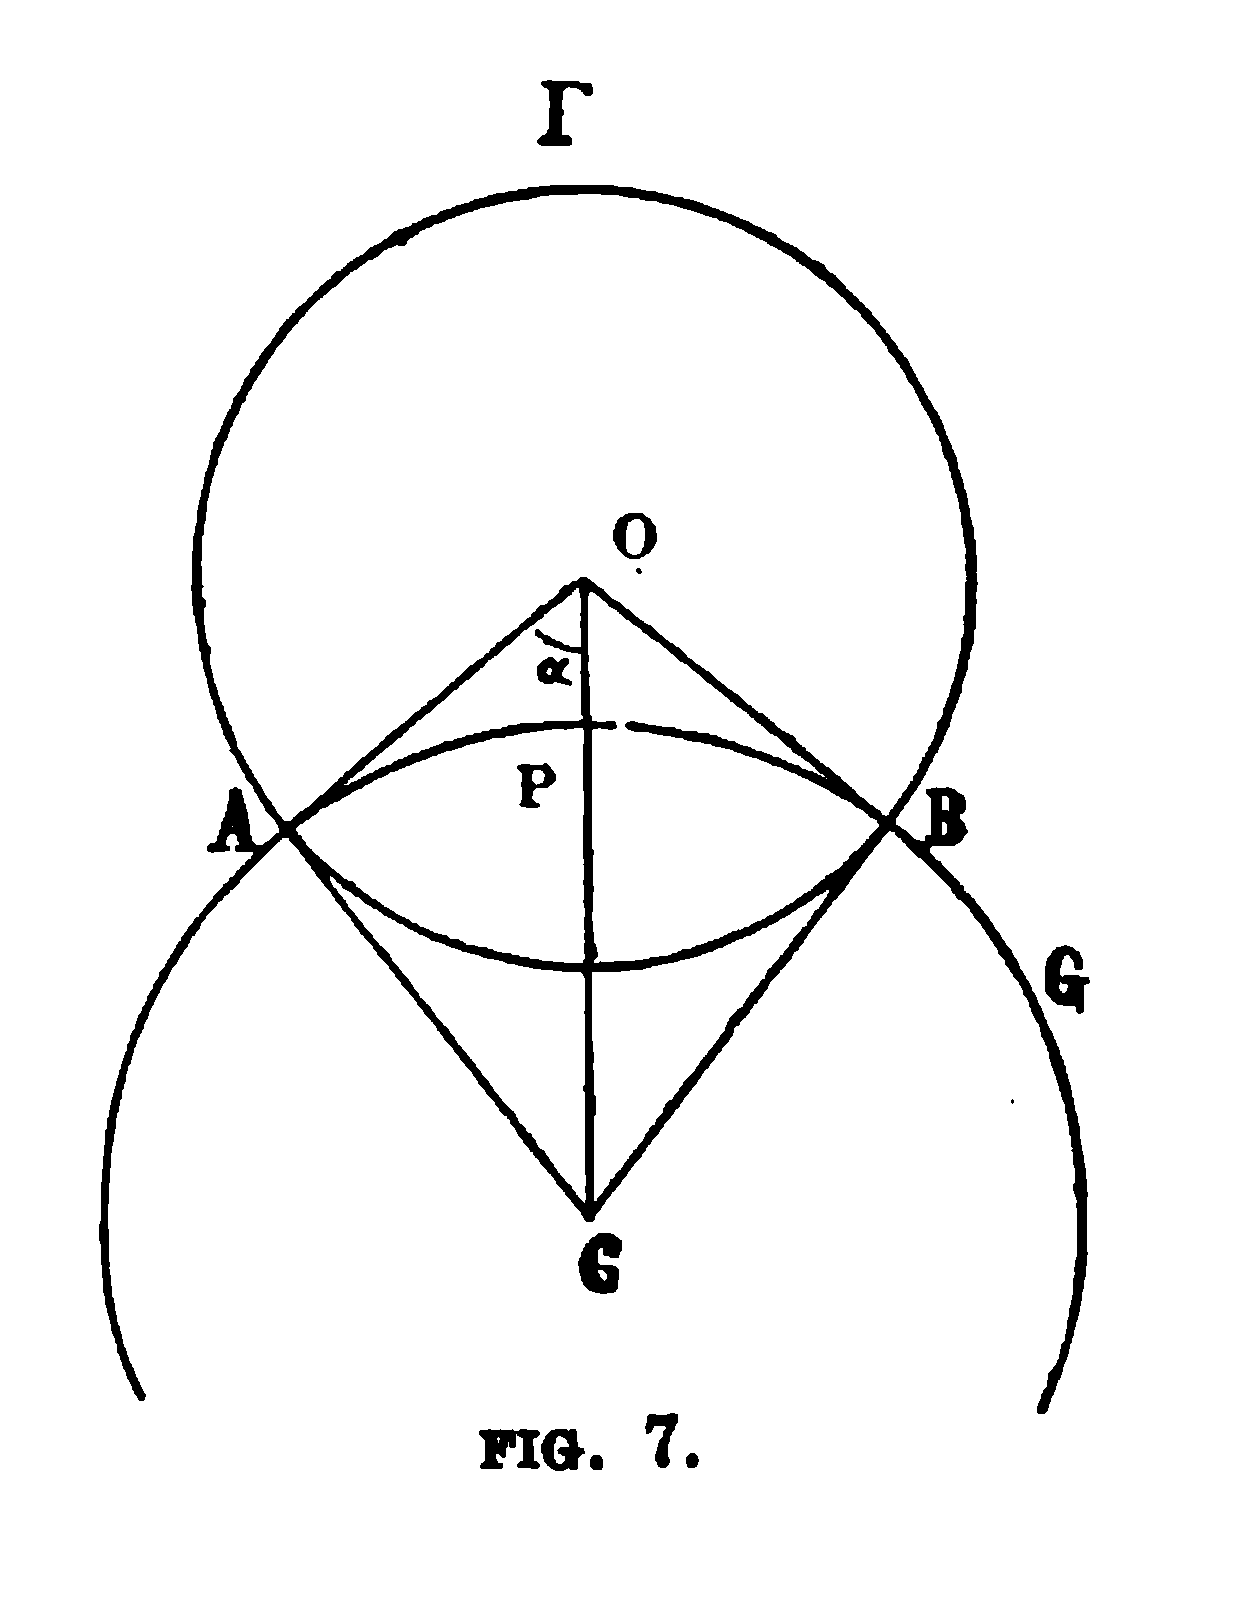
\includegraphics[width=.38\linewidth]{assets/ch12_facsimiles/embedded/Luigi_Bianchi_Geometria_differenziale_Figura_7_facsimile.png}
\end{minipage}\end{center}}
\newcommand{\figsevena}{%
\begin{center}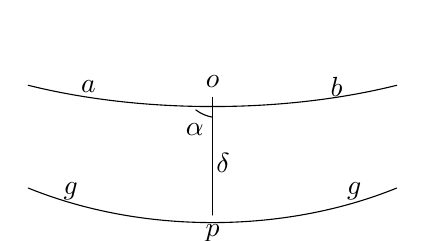
\begin{tikzpicture}[scale=0.9,line cap=round,line join=round]
\draw (-2.6,.65) .. controls (-1,.25) and (1,.25) .. (2.6,.65);
\draw (-2.6,-.8) .. controls (-1,-1.45) and (1,-1.45) .. (2.6,-.8);
\draw (0,.48)--(0,-1.18); \node[above] at (0,.48) {$o$}; \node[below] at (0,-1.18) {$p$};
\node at (-1.75,.63) {$a$}; \node at (1.75,.63) {$b$}; \node at (-2.0,-.85) {$g$}; \node at (2.0,-.85) {$g$};
\draw (0,.2) arc (260:233:.55); \node at (-.25,.03) {$\alpha$}; \node at (.15,-.45) {$\delta$};
\end{tikzpicture}\\[-.2em]{\small Fig. 7a.}\end{center}}
\newcommand{\figeight}{%
\begin{center}\begin{minipage}{.95\linewidth}\centering
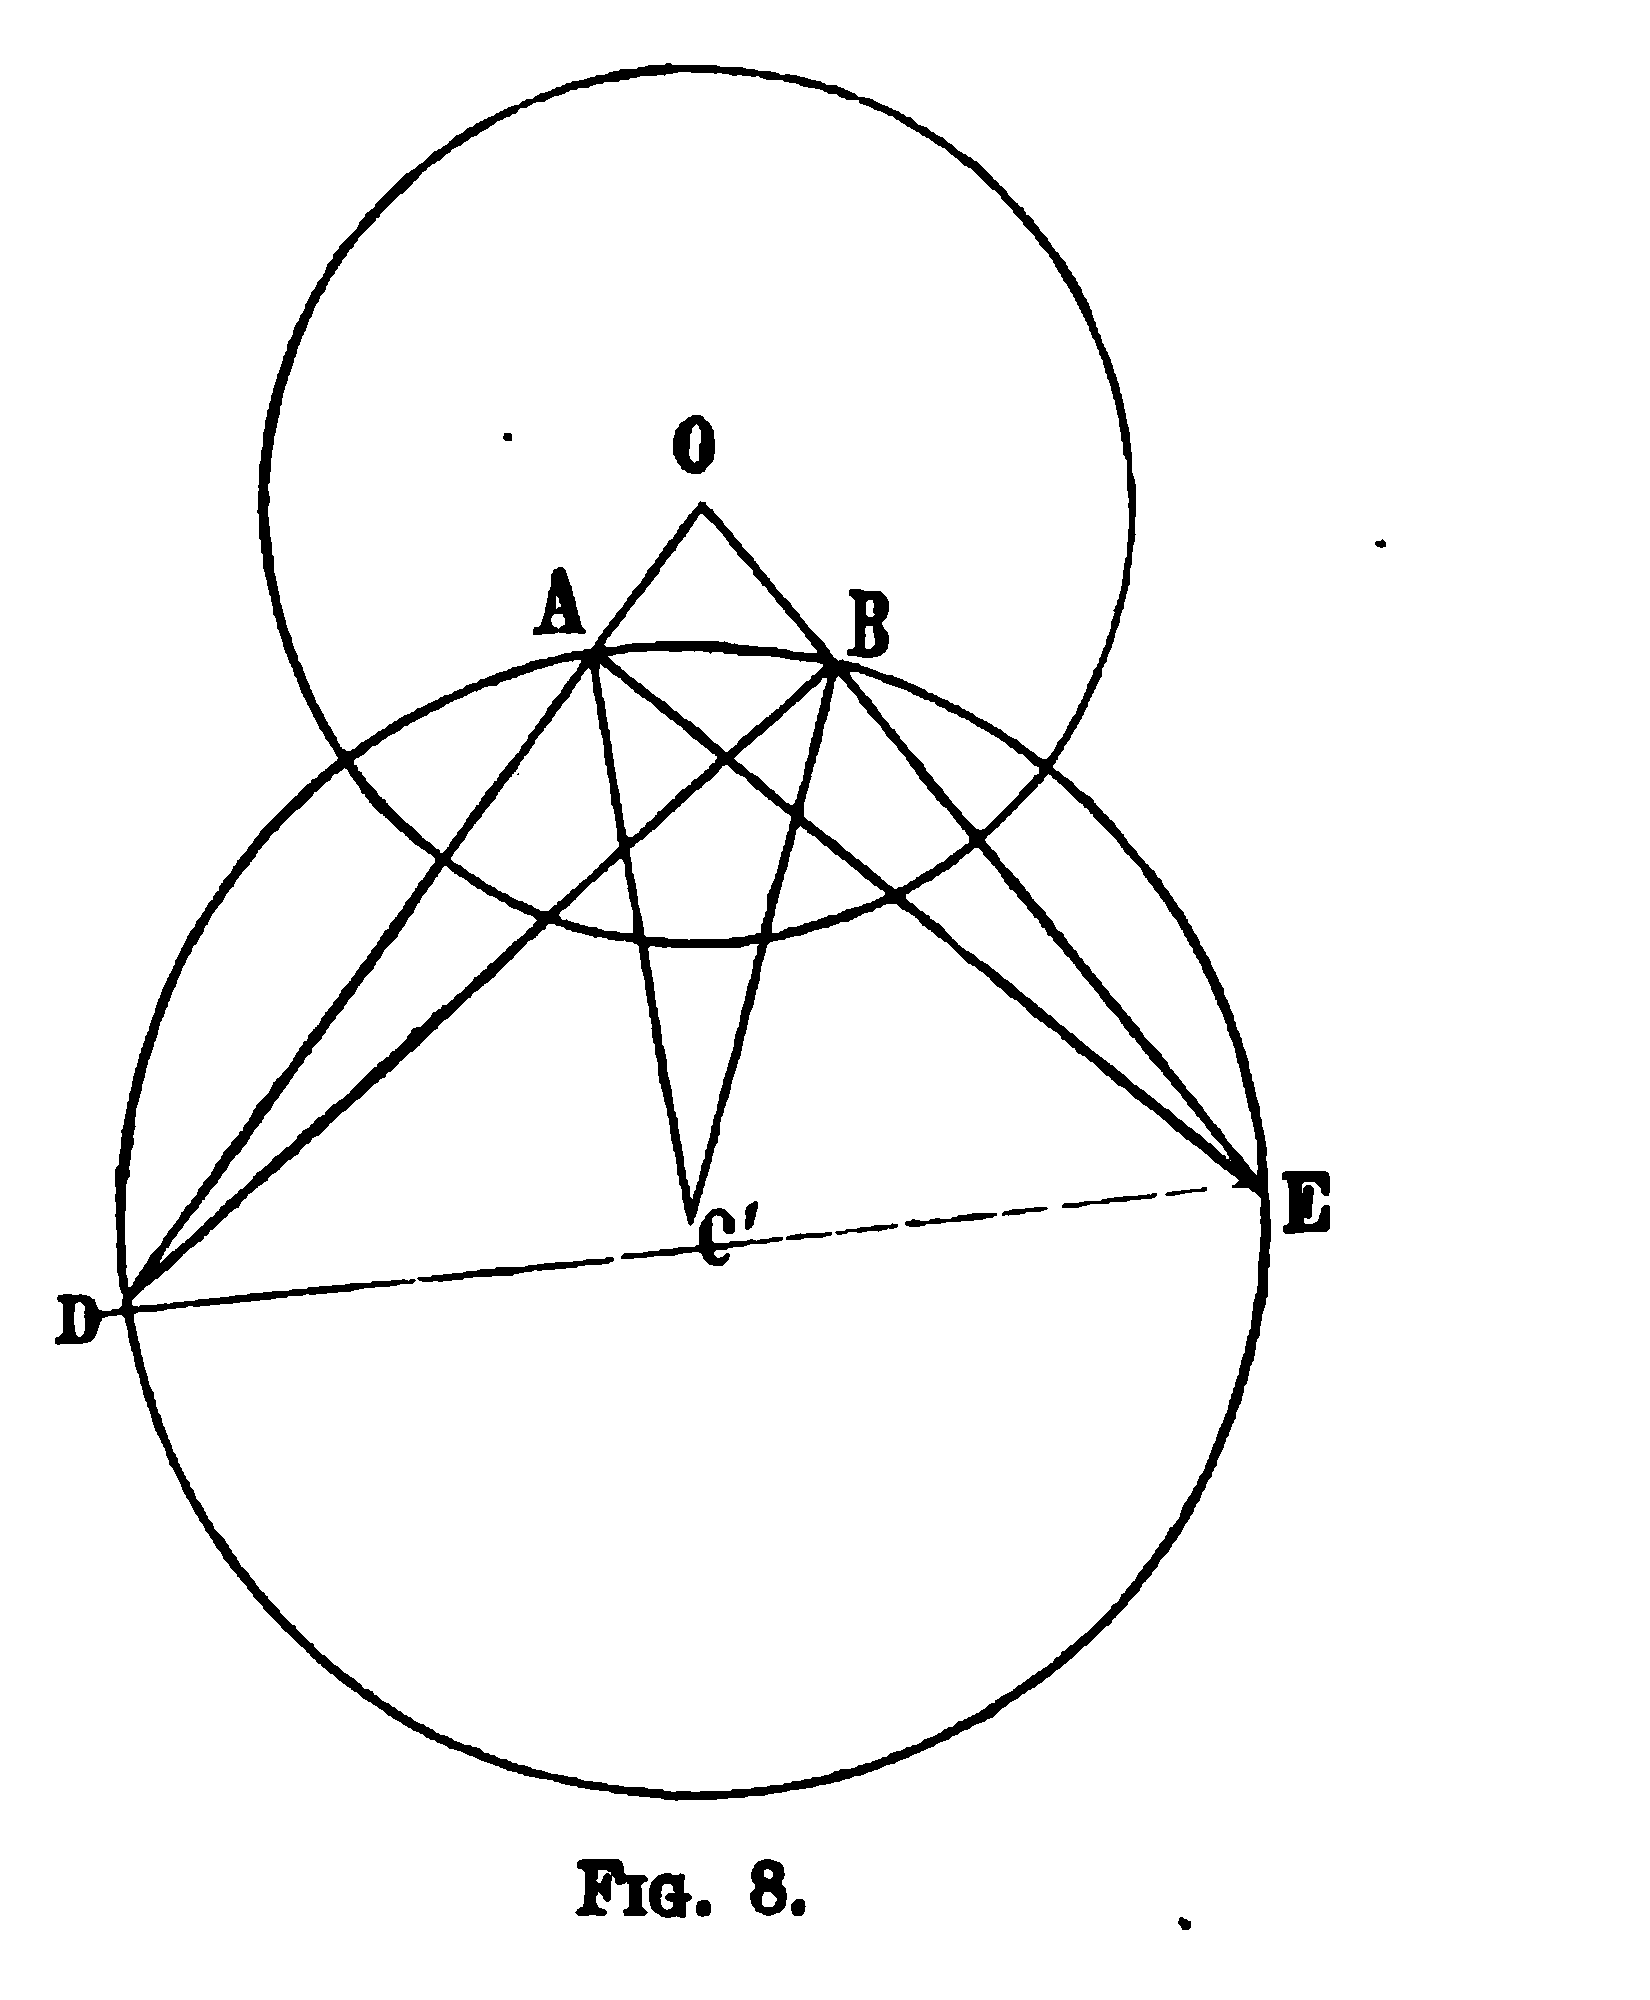
\includegraphics[width=.42\linewidth]{assets/ch12_facsimiles/embedded/Luigi_Bianchi_Geometria_differenziale_Figura_8_facsimile.png}
\end{minipage}\end{center}}
\newcommand{\fignine}{%
\begin{center}\begin{minipage}{.95\linewidth}\centering
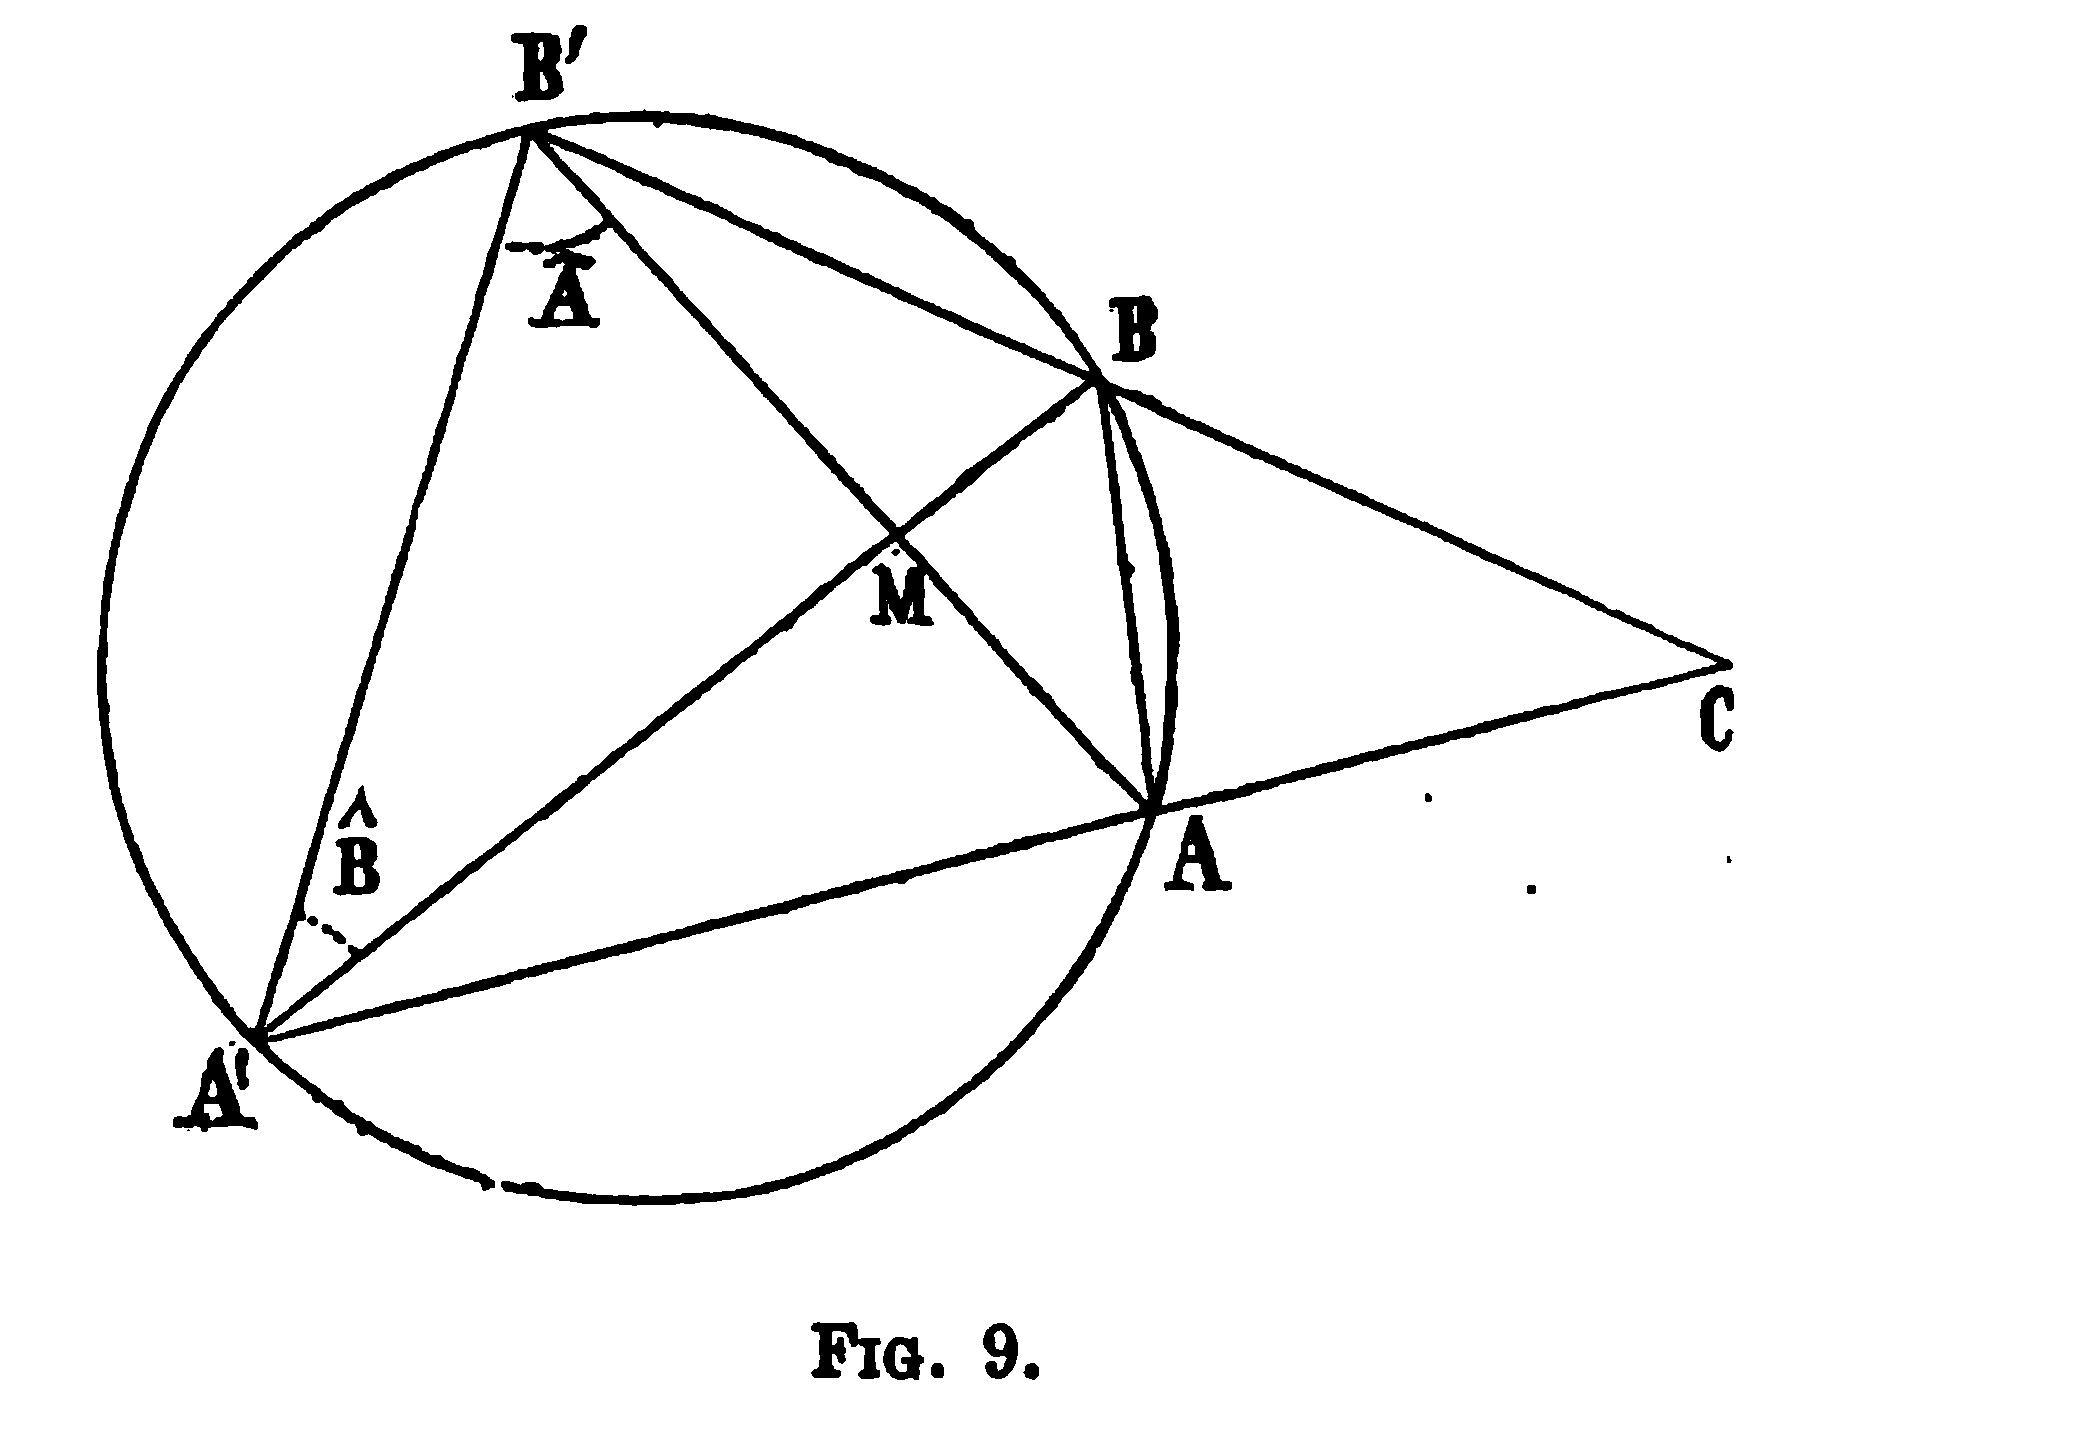
\includegraphics[width=.54\linewidth]{assets/ch12_facsimiles/embedded/Luigi_Bianchi_Geometria_differenziale_Figura_9_facsimile.png}
\end{minipage}\end{center}}


% compatibility shims for p0409--0440 continuation
\providecommand{\sen}{\operatorname{sen}}
\providecommand{\tg}{\operatorname{tg}}
\providecommand{\senh}{\operatorname{senh}}
\providecommand{\tgh}{\operatorname{tgh}}
\providecommand{\cotgh}{\operatorname{cotgh}}
\providecommand{\ang}{\operatorname{ang}}
\providecommand{\grad}{\operatorname{grad}}
\providecommand{\chrB}[2]{\left\{\begin{matrix}#1\\#2\end{matrix}\right\}}
\providecommand{\chrsqB}[2]{\left[\begin{matrix}#1\\#2\end{matrix}\right]}

\begin{document}


\begin{center}
{\bfseries LUIGI BIANCHI}\par
{\small PROFESSOR OF THE ROYAL UNIVERSITY OF PISA}\par
\vspace{1.5em}
{\Huge\bfseries LESSONS}\par
\vspace{1em}
ON\par
\vspace{1em}
{\LARGE\bfseries DIFFERENTIAL GEOMETRY}\par
\vspace{1em}
Second revised and considerably enlarged edition\par
{\bfseries IN TWO VOLUMES}\par
\vspace{1.25em}
{\large\bfseries VOLUME I.}\par
\vspace{4em}
{\large PISA}\par
{\bfseries ENRICO SPOERRI}\par
{\scriptsize BOOKSELLER-PUBLISHER}\par
1902
\end{center}

\begin{center}
{\small Pisa, Tipografia Successori Fratelli Nistri, 1902}
\end{center}

\section*{PREFACE}
The need for a second edition of the present treatise having become evident, I have thought it useful, while preserving in its fundamental lines the general plan of the work, to increase its proportions considerably, so that many parts of the theory, previously confined within too narrow a space, might find a more adequate development in the new treatment. I have also added several new chapters, both to treat theories already relatively old, but which could not be included in the first edition, and to present those quite recent investigations which, it seems, mark the most notable advances made by infinitesimal geometry in recent times.

The bulk of the work, thus doubled, has made division into two volumes necessary, and I have tried to make this correspond approximately to the division of the theories into general and special ones.

The present first volume consists of fourteen chapters, of which the first ten reproduce, with many variations and additions, the corresponding chapters of the first edition, from which I again take the following remarks.

\oldquote
``The method to which the present course is wholly shaped traces its origins to Gauss's celebrated \emph{Disquisitiones generales circa superficies curvas}, and consists in regarding infinitesimal geometry as the study of a quadratic differential form, or of two such simultaneous forms. For this reason, after a first chapter treating curves of double curvature, there will be found a second chapter in which the foundations of the theory of quadratic differential forms are set out, quite briefly.
\closeoldquote

\oldquote
The algorithms deriving from this theory have the great advantage of giving formulae a simple and elegant appearance, easily impressed upon the memory, while preserving for the coordinate lines all their generality; they are used constantly in the sequel of the book, for which this chapter serves as a preliminary.

The general study of surfaces, that is, both of the properties inherent in their actual form in space and of those invariant under bending of the surfaces (theory of applicability), is set out in the following seven chapters (III--IX). Chapter X treats the general theory of the doubly infinite systems of rays (congruences), a theory very important for the general study of surfaces and to which infinitesimal geometry owes many of its most notable results.''
\closeoldquote

The following four chapters reproduce, with greater development and numerous additions, the exposition of the fundamental principles of infinitesimal geometry in \(n\) dimensions which I have already given in the German edition of the book\footnote{\emph{Vorlesungen über Differentialgeometrie} deutsch von M. Lukat (Teubner, Leipzig 1899).}. Chapter XI, after setting the fundamental conventions for the linear and angular metric of an arbitrary \(n\)-dimensional space, introduces the notion of Riemannian curvature and generalizes to curves and hypersurfaces the formulae of ordinary theory, with particular regard to the properties of lines of curvature.

I then pass to treat more particularly spaces of constant Riemannian curvature; and I first deal in Chapter XII (which corresponds to Chapter XVI of the first edition) with two-dimensional pseudospherical geometry, with a brief mention of non-Euclidean geometry.

In the following Chapter XIII I study in general the geometry of \(n\)-dimensional spaces of constant curvature, introduce Cayley's metric and Weierstrass's system of coordinates, and deal particularly with the analytic representation and the properties of motions in three-dimensional spaces, ending with the important notion of Clifford paral-

\noindent lelism in elliptic space and with the extension of Frenet's formulae for curves to elliptic and hyperbolic geometry.

Finally, in Chapter XIV the general theories are applied to the study of hypersurfaces in \(n\)-dimensional spaces of constant curvature, with particular regard to the three-dimensional case, where all the principal results already known for Euclidean space are extended.

To my colleague Prof. O. Niccoletti\ednote{The authority scan spells the surname with two consecutive \emph{c}'s. Earlier digital layers silently normalized it to ``Nicoletti.''}, who kindly assisted me in the final revision of the proofs, I here offer my sincerest thanks.

\begin{flushleft}
\emph{Pisa, April 1902.}
\end{flushleft}

\section*{CHAPTER I.}
\begin{center}
{\Large\bfseries Curves of Double Curvature}
\end{center}

\begin{center}\footnotesize
Tangent and normal plane. -- First curvature or flexion. -- Osculating plane. -- Principal trihedron. -- Second curvature or torsion. -- Frenet formulae. -- Intrinsic equations. -- Cylindrical helices. -- Envelope surfaces. -- Canal surfaces. -- Developable surfaces. -- Rectifying developable and polar developable of a curve. -- Edge of regression of the polar developable. -- Involutes and evolutes. -- Orthogonal trajectories of a simple infinity of planes. -- Combescure transformation. -- Curves of constant flexion and spherical helix. -- Orthogonal trajectories of a simple infinity of spheres. -- Bertrand curves.
\end{center}

\subsection*{§. 1.\quad Tangent and normal plane.}
To define a curve \(C\) analytically, let us refer it to a system of orthogonal Cartesian axes \(Ox, Oy, Oz\), and express the coordinates \(x, y, z\) of a moving point on the curve as functions of a parameter \(u\):
\[
  x=x(u), \qquad y=y(u), \qquad z=z(u).
\]
With respect to the functions \(x(u),y(u),z(u)\), we state once and for all that they are assumed to be \emph{finite and continuous together with their first, second, and third derivatives throughout the interval for the independent variable \(u\) in which they are defined, except at most for special points}.

To every particular value \(u_1\) assigned to the parameter \(u\) within the interval considered there corresponds a particular position \(M_1\) of the point \(M\) generating the curve; and, as \(u\) varies continuously, the point \(M\) will move continuously in space, describing the curve \(C\). We shall always suppose that the sense in which the generating point \(M\) moves when the parameter \(u\) increases is taken as the positive sense of the curve \(C\), and the opposite as negative.

Most often we shall take as parameter or auxiliary variable \(u\) the arc \(s\) of the curve \(C\), counted from a fixed point (origin) on the curve. In any case, to define \(s\) as a function of \(u\), we have the

\noindent well-known formula:
\[
\frac{\diff s}{\diff u}=\sqrt{\left(\frac{\diff x}{\diff u}\right)^2+\left(\frac{\diff y}{\diff u}\right)^2+\left(\frac{\diff z}{\diff u}\right)^2},
\]
where, fixing \(s\) to be counted in the increasing sense of \(u\), we must choose the positive sign for the radical.

At a point \(M\) of the curve \(C\) consider the tangent, whose positive direction is assumed to agree with the positive sense of the curve. Denoting, as we shall do constantly below, by \(\alpha,\beta,\gamma\) the direction cosines of the positive direction of the tangent, we shall have the formulae
\[
\alpha=\frac{\dfrac{\diff x}{\diff u}}{\sqrt{\left(\dfrac{\diff x}{\diff u}\right)^2+\left(\dfrac{\diff y}{\diff u}\right)^2+\left(\dfrac{\diff z}{\diff u}\right)^2}},\qquad
\beta=\frac{\dfrac{\diff y}{\diff u}}{\sqrt{\left(\dfrac{\diff x}{\diff u}\right)^2+\left(\dfrac{\diff y}{\diff u}\right)^2+\left(\dfrac{\diff z}{\diff u}\right)^2}},
\]
\[
\gamma=\frac{\dfrac{\diff z}{\diff u}}{\sqrt{\left(\dfrac{\diff x}{\diff u}\right)^2+\left(\dfrac{\diff y}{\diff u}\right)^2+\left(\dfrac{\diff z}{\diff u}\right)^2}},
\]
or
\begin{equation}\tag{1}
\alpha=\frac{\diff x}{\diff s},\qquad \beta=\frac{\diff y}{\diff s},\qquad \gamma=\frac{\diff z}{\diff s}.
\end{equation}
In these formulae (1), it is immaterial whether the right-hand sides are considered as quotients of differentials or as derivatives taken with respect to the arc.

The plane normal at \(M\) to the tangent is called the normal plane of the curve; it has equation
\[
(X-x)\alpha+(Y-y)\beta+(Z-z)\gamma=0,
\]
where \(X,Y,Z\) denote the current coordinates of a point.

\subsection*{§. 2.\quad First curvature or flexion.}
From the more or less rapid deviation which the point describing the curve undergoes from the rectilinear direction, we judge the greater or lesser \emph{flexion} of the curve itself. To make this concept precise and render it

\noindent susceptible of measurement, consider a point \(M\) of the curve and a nearby point \(M_1\); if we divide the very small angle \(\Delta\varepsilon\) formed by the directions of the two tangents at \(M,M_1\) by the arc length \(MM_1=\Delta s\), the quotient \(\Delta\varepsilon/\Delta s\), when \(M_1\) approaches \(M\) indefinitely (that is, when \(\Delta s\) tends to zero), tends to a determined finite limit, which is taken as the measure of the \emph{first curvature or flexion} of the curve at \(M\). We shall denote this limit by \(1/\rho\), and its inverse \(\rho\), interpreted as a length, will be called the \emph{radius of first curvature}.

To prove the existence of this limit and at the same time find its expression, we use the following considerations.

With center at the origin and radius equal to unity, describe a sphere, and let its surface cut the rays drawn parallel to the positive directions of the successive tangents of the curve. The locus of the endpoints of these rays will be called the \emph{spherical indicatrix} of the tangents; to every position of the generating point \(M=(x,y,z)\) on the curve \(C\) there corresponds a point \(M'=(x',y',z')\) on the spherical indicatrix \(C'\) of the tangents, and evidently one has
\begin{equation}\tag{2}
x'=\alpha,\qquad y'=\beta,\qquad z'=\gamma.
\end{equation}
Now, if we consider a point \(M_1\) of the curve \(C\) near \(M\), the angle \(\Delta\varepsilon\) will be measured precisely by the arc of the great circle which, on the representing sphere, joins the image-points \(M',M'_1\). Since the limit to be calculated is
\[
\frac{1}{\rho}=\lim_{\Delta s\to0}\left(\frac{\Delta\varepsilon}{\Delta s}\right),
\]
we may replace \(\Delta\varepsilon\) by the corresponding arc of the indicatrix, which, for \(\Delta s\) tending to zero, is an infinitesimal whose ratio to \(\Delta\varepsilon\) tends to unity. Denoting by \(\diff s'\) the elementary arc of the spherical indicatrix, we therefore have directly
\[
\frac{1}{\rho}=\frac{\diff s'}{\diff s},
\]
or, by (2),
\begin{equation}\tag{3}
\frac{1}{\rho}=\sqrt{\left(\frac{\diff\alpha}{\diff s}\right)^2+\left(\frac{\diff\beta}{\diff s}\right)^2+\left(\frac{\diff\gamma}{\diff s}\right)^2}.
\end{equation}

If \(s\) is taken as the independent variable, this formula may be written, by (1), as
\begin{equation}\tag{3*}
\frac{1}{\rho}=\sqrt{\left(\frac{\diff^2x}{\diff s^2}\right)^2+\left(\frac{\diff^2y}{\diff s^2}\right)^2+\left(\frac{\diff^2z}{\diff s^2}\right)^2}.
\end{equation}
In these formulae, \emph{agreeing to attribute to the first curvature only an absolute value}, we shall always understand the positive value of the radical to be chosen.

Let us observe at once that a curve \(C\) cannot have zero flexion along an \emph{interval} without being rectilinear along that interval. Indeed, from the resulting equations
\[
\frac{\diff\alpha}{\diff s}=0,\qquad \frac{\diff\beta}{\diff s}=0,\qquad \frac{\diff\gamma}{\diff s}=0,
\]
one would have \(\alpha,\beta,\gamma\) constant, and therefore the formulae
\[
x=\alpha s+a,\qquad y=\beta s+b,\qquad z=\gamma s+c,
\]
with \(a,b,c\) constant, which define a straight line.

\subsection*{§. 3.\quad Osculating plane.}
Among all the planes passing through the point \(M\) of the curve \(C\), there is one which, in a neighborhood of \(M\), departs less from the curve \(C\) than any other plane, and is called the \emph{osculating plane} at \(M\) to the curve. Indeed, write the equation of any plane through \(M=(x,y,z)\) in the form
\begin{equation}\tag{4}
a(X-x)+b(Y-y)+c(Z-z)=0,
\end{equation}
where \(a,b,c\) denote the direction cosines of the normal to the plane. Taking as parameter \(u\) the arc \(s\) of the curve, consider a point \(M'\) near \(M\), corresponding to the value \(s+h\) of the arc, where \(h\) is to be regarded as an infinitesimal of the first order. If \(\Delta x,\Delta y,\Delta z\) are the corresponding increments of \(x,y,z\) in passing from \(s\) to \(s+h\), then for the distance \(\delta\) of the point \(M'\) from the plane (4) we shall have
\[
\delta=a\Delta x+b\Delta y+c\Delta z.
\]

Now we have
\begin{equation}\tag{a}
\left\{
\begin{aligned}
\Delta x&=\frac{\diff x}{\diff s}h+\frac{\diff^2x}{\diff s^2}\frac{h^2}{2}+\varepsilon_1,\\
\Delta y&=\frac{\diff y}{\diff s}h+\frac{\diff^2y}{\diff s^2}\frac{h^2}{2}+\varepsilon_2,\\
\Delta z&=\frac{\diff z}{\diff s}h+\frac{\diff^2z}{\diff s^2}\frac{h^2}{2}+\varepsilon_3,
\end{aligned}
\right.
\end{equation}
where \(\varepsilon_1,\varepsilon_2,\varepsilon_3\) are infinitesimals of the \emph{third order}; hence
\[
\delta=\left(a\frac{\diff x}{\diff s}+b\frac{\diff y}{\diff s}+c\frac{\diff z}{\diff s}\right)h+
\left(a\frac{\diff^2x}{\diff s^2}+b\frac{\diff^2y}{\diff s^2}+c\frac{\diff^2z}{\diff s^2}\right)\frac{h^2}{2}+\eta,
\]
where \(\eta\) is an infinitesimal of the third order.

The plane determined by the conditions
\[
a\frac{\diff x}{\diff s}+b\frac{\diff y}{\diff s}+c\frac{\diff z}{\diff s}=0,
\]
\[
a\frac{\diff^2x}{\diff s^2}+b\frac{\diff^2y}{\diff s^2}+c\frac{\diff^2z}{\diff s^2}=0,
\]
the first of which expresses that the said plane passes through the tangent, is therefore the one which, near \(M\), departs less from the curve than all the others. Thus we have proved the existence of the osculating plane, whose equation, by the preceding, we can write in determinant form as follows\footnote{With any independent variable \(u\), the equation of the osculating plane would evidently preserve the same form:
\[
\detmat{X-x & Y-y & Z-z\\ x' & y' & z'\\ x'' & y'' & z''}=0,
\]
the accents indicating differentiation with respect to \(u\).}:
\begin{equation}\tag{5}
\detmat{X-x & Y-y & Z-z\\
\dfrac{\diff x}{\diff s} & \dfrac{\diff y}{\diff s} & \dfrac{\diff z}{\diff s}\\
\dfrac{\diff^2x}{\diff s^2} & \dfrac{\diff^2y}{\diff s^2} & \dfrac{\diff^2z}{\diff s^2}}=0.
\end{equation}

The osculating plane at a point \(M\) of the curve is in general unique and determined.

The only exception occurs for those points where the three minors of the matrix
\[
\left\|\begin{matrix}
\dfrac{\diff x}{\diff s} & \dfrac{\diff y}{\diff s} & \dfrac{\diff z}{\diff s}\\
\dfrac{\diff^2x}{\diff s^2} & \dfrac{\diff^2y}{\diff s^2} & \dfrac{\diff^2z}{\diff s^2}
\end{matrix}\right\|
\]
vanish simultaneously. But since, because of the formulae
\[
\left(\frac{\diff x}{\diff s}\right)^2+\left(\frac{\diff y}{\diff s}\right)^2+\left(\frac{\diff z}{\diff s}\right)^2=1,
\]
\[
\frac{\diff x}{\diff s}\frac{\diff^2x}{\diff s^2}+\frac{\diff y}{\diff s}\frac{\diff^2y}{\diff s^2}+\frac{\diff z}{\diff s}\frac{\diff^2z}{\diff s^2}=0,
\]
the square of this matrix equals, by (3*), the square of the flexion, it is seen that the said singular points are those where the flexion is zero.

We shall also mention other definitions of the osculating plane, which always lead, as is easily seen, to equation (5).

If through the tangent at \(M\) and through a nearby point \(M'\) of \(C\) one passes a plane, this plane, as \(M'\) tends to \(M\), tends to the osculating plane as limiting plane. Again: if through \(M\) and two other nearby points \(M',M''\) one passes a plane, this plane tends to the osculating plane when \(M',M''\) tend simultaneously to \(M\) (in such a way that the differences between the coordinates of \(M',M''\) do not become infinitesimals of higher order with respect to the corresponding differences from \(M\)). By this last property it is also said, in abbreviated form, that the osculating plane at a point is the plane drawn through this point and two successive points on the curve.

\subsection*{§. 4.\quad Principal trihedron.}
Among all the normals at \(M\) to the curve, the \emph{principal normal} is the one lying in the osculating plane, that is, the line of intersection of the osculating plane with the normal plane. The \emph{binormal} of the curve is the normal to the osculating plane.

We have already fixed the positive direction of the tangent; it is now convenient to fix, by suitable conventions, the positive directions of the principal normal and of the binormal. These three positive directions determine a trirectangular trihedron, which we shall call the \emph{principal trihedron} of the curve, relative to the point \(M\) under consideration.

We shall henceforth denote constantly by
\[
\xi,\ \eta,\ \zeta
\]
the direction cosines of the (positive) principal normal, and by
\[
\lambda,\ \mu,\ \nu
\]
those of the binormal. From equation (5) of the osculating plane there follow at once the proportions
\[
\lambda:\mu:\nu=
\detmat{\dfrac{\diff y}{\diff s} & \dfrac{\diff z}{\diff s}\\[0.6em]
\dfrac{\diff^2y}{\diff s^2} & \dfrac{\diff^2z}{\diff s^2}}
:
\detmat{\dfrac{\diff z}{\diff s} & \dfrac{\diff x}{\diff s}\\[0.6em]
\dfrac{\diff^2z}{\diff s^2} & \dfrac{\diff^2x}{\diff s^2}}
:
\detmat{\dfrac{\diff x}{\diff s} & \dfrac{\diff y}{\diff s}\\[0.6em]
\dfrac{\diff^2x}{\diff s^2} & \dfrac{\diff^2y}{\diff s^2}},
\]
and consequently (since \(\xi\alpha+\eta\beta+\zeta\gamma=0,\ \xi\lambda+\eta\mu+\zeta\nu=0\)):
\[
\xi:\eta:\zeta=\frac{\diff^2x}{\diff s^2}:\frac{\diff^2y}{\diff s^2}:\frac{\diff^2z}{\diff s^2};
\]
whence, by (3*), we deduce
\begin{equation}\tag{6}
\xi=\pm\rho\frac{\diff^2x}{\diff s^2},\qquad
\eta=\pm\rho\frac{\diff^2y}{\diff s^2},\qquad
\zeta=\pm\rho\frac{\diff^2z}{\diff s^2}.
\end{equation}
Now consider the plane of the tangent and the binormal, whose equation is
\begin{equation}\tag{7}
(X-x)\xi+(Y-y)\eta+(Z-z)\zeta=0,
\end{equation}
and let us calculate the distance \(\delta\) from this plane to a point \(M'\) of the curve near \(M\). With the notation of §. 3 we shall have
\[
\delta=\xi\Delta x+\eta\Delta y+\zeta\Delta z,
\]
and, as is well known from analytic geometry, \(\delta\) will be positive or negative according as \(M'\) lies on the positive or negative side of the plane (7), that is, in the region toward which the positive direction

\noindent \((\xi,\eta,\zeta)\) of the normal to the plane is turned, or in the opposite one. Now, applying formulae (a) on page 5, and observing (6), we obtain
\begin{equation}\tag{8}
\delta=\pm\frac{h^2}{2\rho}+\eta,
\end{equation}
where \(\eta\) denotes an infinitesimal of the third order. From this formula the sign of \(\delta\) is independent of that of \(h\), whence one sees that: \emph{In the neighborhood of each of its points the curve lies entirely on one side of the plane of the tangent and the binormal}\footnote{The singular points at which the flexion is zero must be excluded.}. We shall take as the positive side of this plane the one which, near \(M\), is turned toward the curve, and consequently the positive direction of the principal normal will thereby be fixed. Under this convention the sign of \(\delta\) in (8) must be positive, and therefore the sign to be adopted in (6) is the upper one. We thus have the definitive formulae
\begin{equation}\tag{9}
\xi=\rho\frac{\diff^2x}{\diff s^2},\qquad
\eta=\rho\frac{\diff^2y}{\diff s^2},\qquad
\zeta=\rho\frac{\diff^2z}{\diff s^2}.
\end{equation}
Finally, we agree to fix as the positive direction \((\lambda,\mu,\nu)\) of the binormal the one which stands, with respect to the already fixed positive directions of the tangent and principal normal, as the positive direction of the \(Oz\)-axis stands with respect to those of the \(Ox,Oy\)-axes. The determinant
\[
\detmat{\alpha & \beta & \gamma\\
\xi & \eta & \zeta\\
\lambda & \mu & \nu}
\]
of the nine cosines of the three principal directions will then be equal to positive unity, and each of its elements will equal its own algebraic cofactor. Thus one has
\begin{equation}\tag{10}
\left\{
\begin{aligned}
\lambda&=\beta\zeta-\gamma\eta=\rho\left(\frac{\diff y}{\diff s}\frac{\diff^2z}{\diff s^2}-\frac{\diff z}{\diff s}\frac{\diff^2y}{\diff s^2}\right),\\[0.4em]
\mu&=\gamma\xi-\alpha\zeta=\rho\left(\frac{\diff z}{\diff s}\frac{\diff^2x}{\diff s^2}-\frac{\diff x}{\diff s}\frac{\diff^2z}{\diff s^2}\right),\\[0.4em]
\nu&=\alpha\eta-\beta\xi=\rho\left(\frac{\diff x}{\diff s}\frac{\diff^2y}{\diff s^2}-\frac{\diff y}{\diff s}\frac{\diff^2x}{\diff s^2}\right).
\end{aligned}\right.
\end{equation}


\subsection*{§. 5.\quad Second curvature, or torsion.}
The osculating plane of a curve \(C\) in general varies as the point \(M\) of osculation varies, and the rapidity of its deviation, that is, of the departure of the curve from plane position, is measured by the \emph{second curvature, or torsion}.

To make this concept precise here also, we shall consider a point \(M\) of the curve and a neighboring point \(M_1\); the two osculating planes at \(M,M_1\) will contain between them a very small angle \(\Delta\sigma\), and the quotient \(\Delta\sigma/\Delta s\), where \(\Delta s\) denotes the arc \(MM_1\), will converge, as \(\Delta s\) tends to zero, toward a determinate and finite limit, which will be taken as the measure of the \emph{torsion} of the curve and, with a convenient sign, will be denoted by \(1/T\); its inverse \(T\) will be called the radius of second curvature. To find the expression of \(1/T\), let us begin by observing that this angle \(\Delta\sigma\) is measured by the angle of the two successive binormals at \(M,M_1\). If, therefore, in a wholly analogous way to §. 3, we construct the \emph{spherical indicatrix of the binormals}, whose generating point has coordinates
\[
 x_1=\lambda,\qquad y_1=\mu,\qquad z_1=\nu,
\]
and if by \(\diff s_1\) we denote its element of arc
\[
\diff s_1=\sqrt{\diff x_1^2+\diff y_1^2+\diff z_1^2},
\]
we shall manifestly have
\begin{equation}\tag{11}
\frac{1}{T}=\pm\frac{\diff s_1}{\diff s}=\pm\sqrt{\left(\frac{\diff\lambda}{\diff s}\right)^2+\left(\frac{\diff\mu}{\diff s}\right)^2+\left(\frac{\diff\nu}{\diff s}\right)^2}.
\end{equation}
We shall fix the sign of the torsion in the most convenient way in the next §; meanwhile let us observe that the only curves of zero torsion are plane curves. Indeed, if \(1/T=0\), it follows from (11) that \(\lambda,\mu,\nu\) are constant. If, therefore, for simplicity, we take the fixed direction of the binormal as the axis of the \(z\)'s, we shall have
\[
\lambda=0,
\qquad \mu=0,
\qquad \nu=1,
\]
hence \(\gamma=0\), and therefore \(z=\) constant; thus the curve will be traced in a plane parallel to the plane \(xy\).

\subsection*{§. 6.\quad Formulae of Frenet.}
We shall now establish the important formulae which express the derivatives (taken with respect to arc) of the nine cosines of the three principal directions in terms of the cosines themselves and of the radii \(\rho,T\) of first and second curvature. Three of them result immediately from (9), §. 4 (p. 8), which give
\begin{equation}\tag{a}
\frac{\diff\alpha}{\diff s}=\frac{\xi}{\rho},\qquad
\frac{\diff\beta}{\diff s}=\frac{\eta}{\rho},\qquad
\frac{\diff\gamma}{\diff s}=\frac{\zeta}{\rho}.
\end{equation}
Now, if we differentiate with respect to \(s\) the two identities
\[
\alpha\lambda+\beta\mu+\gamma\nu=0,
\]
\[
\lambda^2+\mu^2+\nu^2=1,
\]
and observe the preceding (a), we deduce
\[
\left\{
\begin{aligned}
\alpha\frac{\diff\lambda}{\diff s}+\beta\frac{\diff\mu}{\diff s}+\gamma\frac{\diff\nu}{\diff s}&=0,\\[0.4em]
\lambda\frac{\diff\lambda}{\diff s}+\mu\frac{\diff\mu}{\diff s}+\nu\frac{\diff\nu}{\diff s}&=0,
\end{aligned}\right.
\]
and therefore the proportions
\[
\frac{\diff\lambda}{\diff s}:\frac{\diff\mu}{\diff s}:\frac{\diff\nu}{\diff s}=
\detmat{\beta&\gamma\\ \mu&\nu}:
\detmat{\gamma&\alpha\\ \nu&\lambda}:
\detmat{\alpha&\beta\\ \lambda&\mu},
\]
that is,
\[
\frac{\diff\lambda}{\diff s}:\frac{\diff\mu}{\diff s}:\frac{\diff\nu}{\diff s}=\xi:\eta:\zeta.
\]
Thus the three ratios
\[
\frac{1}{\xi}\frac{\diff\lambda}{\diff s},\qquad
\frac{1}{\eta}\frac{\diff\mu}{\diff s},\qquad
\frac{1}{\zeta}\frac{\diff\nu}{\diff s}
\]
are equal; their absolute value evidently equals the value
\[
\sqrt{\left(\frac{\diff\lambda}{\diff s}\right)^2+\left(\frac{\diff\mu}{\diff s}\right)^2+\left(\frac{\diff\nu}{\diff s}\right)^2}=\pm\frac{1}{T}.
\]

We shall fix the sign of the torsion by assuming
\[
\frac{1}{T}=\frac{1}{\xi}\frac{\diff\lambda}{\diff s}=\frac{1}{\eta}\frac{\diff\mu}{\diff s}=\frac{1}{\zeta}\frac{\diff\nu}{\diff s};
\]
and we shall have
\begin{equation}\tag{a'}
\frac{\diff\lambda}{\diff s}=\frac{\xi}{T},\qquad
\frac{\diff\mu}{\diff s}=\frac{\eta}{T},\qquad
\frac{\diff\nu}{\diff s}=\frac{\zeta}{T}.
\end{equation}
Thus there will be attributed to the torsion not only an absolute value but also an algebraic value, and it remains to examine, which we shall do shortly, to what geometrical circumstance the positive or negative sign of the torsion corresponds.

We complete formulae (a), (a') with those relative to the derivatives
\[
\frac{\diff\xi}{\diff s},\qquad \frac{\diff\eta}{\diff s},\qquad \frac{\diff\zeta}{\diff s}.
\]
If we observe, for example, that one has
\[
\xi=\gamma\mu-\beta\nu
\]
and differentiate, observing (a), (a'), we obtain
\[
\frac{\diff\xi}{\diff s}=\frac{1}{\rho}(\zeta\mu-\eta\nu)+\frac{1}{T}(\gamma\eta-\beta\zeta),
\]
that is,
\[
\frac{\diff\xi}{\diff s}=-\frac{\alpha}{\rho}-\frac{\lambda}{T},
\]
and analogously for the other two derivatives. Summarizing the formulae obtained, we have the following table:
\begin{equation}\tag{A}
\left\{
\begin{aligned}
\frac{\diff\alpha}{\diff s}&=\frac{\xi}{\rho},&
\frac{\diff\beta}{\diff s}&=\frac{\eta}{\rho},&
\frac{\diff\gamma}{\diff s}&=\frac{\zeta}{\rho},\\[0.4em]
\frac{\diff\xi}{\diff s}&=-\frac{\alpha}{\rho}-\frac{\lambda}{T},&
\frac{\diff\eta}{\diff s}&=-\frac{\beta}{\rho}-\frac{\mu}{T},&
\frac{\diff\zeta}{\diff s}&=-\frac{\gamma}{\rho}-\frac{\nu}{T},\\[0.4em]
\frac{\diff\lambda}{\diff s}&=\frac{\xi}{T},&
\frac{\diff\mu}{\diff s}&=\frac{\eta}{T},&
\frac{\diff\nu}{\diff s}&=\frac{\zeta}{T}.
\end{aligned}\right.
\end{equation}
These are the formulae of \textsc{Frenet}, more commonly known under the name of the formulae of \textsc{Serret}.

\subsection*{§. 7.\quad Sign of the torsion.}
Let us now examine what geometrical meaning is possessed by the positive or negative sign of the torsion, which already from formulae (A) in the last line proves to be independent of the positive sense of traversal on the curve \(C\), since, when this is changed into the opposite, \(\xi,\eta,\zeta\) do not change, while \(\lambda,\mu,\nu\) change sign together with the positive sense of \(s\).

For our purpose let us calculate, up to infinitesimals of the third order, the distance \(\delta\) of a point \(M'\) of the curve near \(M\) from the osculating plane at \(M\), whose equation is
\[
(X-x)\lambda+(Y-y)\mu+(Z-z)\nu=0.
\]
With the usual notation of the preceding §§ we shall have
\[
\delta=\lambda\Delta x+\mu\Delta y+\nu\Delta z;
\]
now one has
\[
\left\{
\begin{aligned}
\Delta x&=\frac{\diff x}{\diff s}h+\frac{\diff^2x}{\diff s^2}\frac{h^2}{2}+\frac{\diff^3x}{\diff s^3}\frac{h^3}{6}+\varepsilon_1,\\[0.4em]
\Delta y&=\frac{\diff y}{\diff s}h+\frac{\diff^2y}{\diff s^2}\frac{h^2}{2}+\frac{\diff^3y}{\diff s^3}\frac{h^3}{6}+\varepsilon_2,\\[0.4em]
\Delta z&=\frac{\diff z}{\diff s}h+\frac{\diff^2z}{\diff s^2}\frac{h^2}{2}+\frac{\diff^3z}{\diff s^3}\frac{h^3}{6}+\varepsilon_3,
\end{aligned}\right.
\]
where \(\varepsilon_1,\varepsilon_2,\varepsilon_3\) are infinitesimals of order higher than the third with respect to \(h\). From the formulae of Frenet, on the other hand, there results
\[
\frac{\diff x}{\diff s}=\alpha,
\qquad
\frac{\diff^2x}{\diff s^2}=\frac{\xi}{\rho},
\qquad
\frac{\diff^3x}{\diff s^3}=-\frac{1}{\rho}\left\{\frac{\alpha}{\rho}+\frac{\lambda}{T}+\frac{\xi}{\rho}\frac{\diff\rho}{\diff s}\right\}
\]
and therefore
\[
\delta=-\frac{1}{6\rho T}h^3+\eta,
\]
where \(\eta/h^3\) is infinitesimal with \(h\). Supposing that the two curvatures \(1/\rho,1/T\) are not zero at \(M\), one sees that the sign of \(\delta\) changes with the sign of \(h\), that is: \emph{the curve crosses the osculating plane at \(M\)}. More precisely, the preceding formula shows that if \(1/T>0\) the generating point,

\noindent moving in the positive sense on the curve, passes from the positive face to the negative face of the osculating plane, and the opposite occurs for \(1/T<0\). It follows also from this that the sign of the torsion is independent of the positive sense chosen on the curve, since, when this is reversed, the two sides, positive and negative, of the osculating plane are likewise interchanged.

To express our result more concisely, imagine an observer placed at \(M\) on one or the other face of the osculating plane and facing toward the positive direction of the principal normal. The curve, in \emph{rising} with respect to the observer, passes at \(M\) from left to right or from right to left; in the first case one will say that at \(M\) the curve is right-handed, in the second left-handed.

And now, if we fix once for all that on the positive side of the plane \(xy\) the positive direction \(Oy\) lies to the left of \(Ox\), we see at once that: \emph{The torsion of a curve \(C\), calculated by the formulae of Frenet, will be positive or negative according as at the point considered the curve \(C\) is left-handed or right-handed.}

\subsection*{§. 8.\quad Intrinsic equations.}
We can immediately apply the formulae of Frenet to the proof of the important theorem: \emph{A skew curve \(C\) is completely determined in form by the expressions of the two curvatures \(1/\rho\), \(1/T\) as functions of arc.}

In other words, we say that if two curves \(C,C'\), with equal arc, have equal flexions as well as equal torsions, they are superposable. Denoting by accents the quantities relative to \(C'\), we shall meanwhile have as hypothesis
\[
s'=s,
\qquad \rho'=\rho,
\qquad T'=T.
\]
Now let us move the curve \(C'\) in space so as to superpose one of its points, for example the origin \(s=0\) of the arcs, on the corresponding point of \(C\), and simultaneously its principal trihedron on that of \(C\) at the same point \(s=0\). We shall then have
\[
\left.
\begin{aligned}
\alpha'&=\alpha,& \beta'&=\beta,& \gamma'&=\gamma,\\
\xi'&=\xi,& \eta'&=\eta,& \zeta'&=\zeta,\\
\lambda'&=\lambda,& \mu'&=\mu,& \nu'&=\nu
\end{aligned}
\right\}\quad \hbox{for }s=0.
\]

Write the three Frenet formulae in the first column of table (A) on p. 11, both for the curve \(C\) and for \(C'\):
\[
\frac{\diff\alpha}{\diff s}=\frac{\xi}{\rho},\qquad
\frac{\diff\xi}{\diff s}=-\frac{\alpha}{\rho}-\frac{\lambda}{T},\qquad
\frac{\diff\lambda}{\diff s}=\frac{\xi}{T},
\]
\[
\frac{\diff\alpha'}{\diff s}=\frac{\xi'}{\rho},\qquad
\frac{\diff\xi'}{\diff s}=-\frac{\alpha'}{\rho}-\frac{\lambda'}{T},\qquad
\frac{\diff\lambda'}{\diff s}=\frac{\xi'}{T};
\]
multiplying the first three, respectively, by \(\alpha',\xi',\lambda'\), the second by \(\alpha,\xi,\lambda\), and adding, the second member becomes zero; whence it follows that
\[
\frac{\diff}{\diff s}(\alpha\alpha'+\xi\xi'+\lambda\lambda')=0,
\]
that is,
\[
\alpha\alpha'+\xi\xi'+\lambda\lambda'=\hbox{constant}.
\]
But since initially, for \(s=0\), the value of the first member is unity, we shall have for every value of \(s\):
\[
\alpha\alpha'+\xi\xi'+\lambda\lambda'=1,
\]
which formula, because of the identities
\[
\alpha^2+\xi^2+\lambda^2=1,
\]
\[
\alpha'^2+\xi'^2+\lambda'^2=1,
\]
can be written
\[
(\alpha-\alpha')^2+(\xi-\xi')^2+(\lambda-\lambda')^2=0;
\]
there follows
\[
\alpha'=\alpha,
\qquad \xi'=\xi,
\qquad \lambda'=\lambda.
\]
Similarly we shall deduce
\[
\beta'=\beta,
\qquad \eta'=\eta,
\qquad \mu'=\mu
\]
\[
\gamma'=\gamma,
\qquad \zeta'=\zeta,
\qquad \nu'=\nu,
\]
and therefore
\[
\frac{\diff(x'-x)}{\diff s}=0,
\qquad
\frac{\diff(y'-y)}{\diff s}=0,
\qquad
\frac{\diff(z'-z)}{\diff s}=0.
\]
The differences \(x'-x,y'-y,z'-z\) are therefore constant and, being initially zero, will always be zero; this proves our theorem.

Once the expressions of \(1/\rho\), \(1/T\) as functions of \(s\) are known,
\[
\frac{1}{\rho}=f(s),\qquad \frac{1}{T}=\varphi(s),
\]

\noindent (where, by the conventions already made, the function \(f(s)\) must always be positive), the curve is therefore determined in form without regard to its particular position in space; for this reason the above equations are fittingly called the \emph{intrinsic equations} of the curve.

\subsection*{§. 9.\quad Integration of the intrinsic equations.}
Relying on the theorems which ensure the existence of the integrals of differential equations, we then easily see that: \emph{Given arbitrarily the intrinsic equations
\[
\frac{1}{\rho}=f(s),\qquad \frac{1}{T}=\varphi(s)
\]
of a curve, the corresponding curve actually exists.}

Denoting by \(l,m,n\) three unknown functions of \(s\), let us indeed write the system of the three homogeneous linear equations
\begin{equation}\tag{12}
\frac{\diff l}{\diff s}=m f(s),\qquad
\frac{\diff m}{\diff s}=-l f(s)-n\varphi(s),\qquad
\frac{\diff n}{\diff s}=m\varphi(s),
\end{equation}
of which, if the curve exists, by the formulae of Frenet,
\[
(\alpha,\xi,\lambda),\qquad (\beta,\eta,\mu),\qquad (\gamma,\zeta,\nu)
\]
will be three integral systems. We know from the theory of differential equations that, when the initial values, for example for \(s=0\), of the unknown functions \(l,m,n\) are assigned arbitrarily, there exists an integral system \((l,m,n)\) of (12) which for \(s=0\) reduces to the assigned initial system \((l_0,m_0,n_0)\); moreover, since (12) are linear, the integrals \(l,m,n\) will exist and will be regular throughout that interval for \(s\) in which the assigned functions \(f(s),\varphi(s)\) remain finite and continuous.

We further observe that if \((l,m,n)\), \((l',m',n')\) are two integral systems of (12), distinct or coincident, it follows from the differential equations themselves that
\[
\frac{\diff}{\diff s}(ll'+mm'+nn')=0,
\]
and therefore
\[
ll'+mm'+nn'=\hbox{constant}.
\]

This being settled, let us take nine constants
\[
\begin{matrix}
l_0 & l'_0 & l''_0\\
m_0 & m'_0 & m''_0\\
n_0 & n'_0 & n''_0,
\end{matrix}
\]
which form the coefficients of an orthogonal substitution, and let us denote by
\[
(l,m,n),\qquad (l',m',n'),\qquad (l'',m'',n'')
\]
the three integral systems of (12), which for \(s=0\) reduce respectively to
\[
(l_0,m_0,n_0),\qquad (l'_0,m'_0,n'_0),\qquad (l''_0,m''_0,n''_0).
\]
It follows from the preceding observation that for \emph{all values of \(s\)}
\[
\begin{matrix}
l & l' & l''\\
m & m' & m''\\
n & n' & n''
\end{matrix}
\]
will be the coefficients of an orthogonal substitution; in particular,
\[
l^2+l'^2+l''^2=1.
\]
Now set
\[
x=\int l\,\diff s,
\qquad y=\int l'\,\diff s,
\qquad z=\int l''\,\diff s,
\]
and interpret \(x,y,z\) as the coordinates of a moving point \(M\); the curve, the locus of the point \(M\), will evidently have \(s\) for arc and \(l,l',l''\) for the direction cosines of the tangent. If in addition one takes account of the differential equations (12), which are satisfied by \((l,m,n),(l',m',n'),(l'',m'',n'')\), and of the formulae of Frenet, it is seen at once that the two curvatures \(1/\rho,1/T\) of the curve will have precisely the assigned values
\[
\frac{1}{\rho}=f(s),\qquad \frac{1}{T}=\varphi(s).
\]
Lastly, let us show with Darboux how the integration of the system (12) is reduced to that of a differential equation of Riccati type. For every integral system of (12) one has
\[
l^2+m^2+n^2=\hbox{constant}
\]
and, by multiplying \(l,m,n\) by the same constant factor (thereby obtaining

\noindent a new integral system because of homogeneity), one may suppose without further qualification that
\[
l^2+m^2+n^2=1.
\]
We then express \(l,m,n\) by two angles \(\theta,\varphi\) with the formulae
\[
l=\sen\theta\cos\varphi,
\qquad m=\sen\theta\sen\varphi,
\qquad n=\cos\theta,
\]
and (12) will give for \(\theta,\varphi\) the two simultaneous equations
\begin{equation}\tag{13}
\frac{\diff\theta}{\diff s}+\frac{\sen\varphi}{T}=0,
\qquad
\frac{\diff\varphi}{\diff s}+\frac{\cot\theta\cos\varphi}{T}+\frac{1}{\rho}=0.
\end{equation}
Next introduce, as the single unknown, the complex function
\[
\sigma=\cot\frac{\theta}{2}\,e^{i\varphi}
\]
(to which later (Chap. III) we shall recognize the meaning of a \emph{complex variable on the sphere}); from (13) there will follow for \(\sigma\) the single equation
\refstepcounter{footnote}
\begin{equation}\tag{14}
\frac{\diff\sigma}{\diff s}+\frac{i\sigma^2}{2T}+\frac{i\sigma}{\rho}-\frac{i}{2T}=0^{(\thefootnote)},
\end{equation}
\footnotetext{In the simplest way the calculation is carried out by differentiating \(\sigma\) logarithmically, observing (13), and substituting for \(\sen\varphi,\cos\varphi\) their expressions by means of the exponential.}
from which, conversely, separating the real from the imaginary, (13) follow. Therefore: \emph{The problem of determining a curve from its intrinsic equations is reduced to the integration of equation (14) of Riccati type.}

By known properties of equations of this type, knowledge of a particular solution suffices to ascend by quadratures to the general integral.

As an example, let us consider the case of a \emph{plane} curve determined by its intrinsic equations:
\[
\frac{1}{\rho}=f(s),\qquad \frac{1}{T}=0.
\]
Then (14), or else (13), is immediately integrated. It is clear that \(\theta\) will have a constant value and, without altering generality, we may take \(\theta=\pi/2\); hence by the quadrature
\begin{equation}\tag{15}
\varphi=-\int f(s)\,\diff s
\end{equation}


\noindent one will obtain \(\varphi\). For the required curve we shall finally have
\begin{equation}\tag{15*}
x=a+\int \cos\varphi\,\diff s,\qquad y=b+\int \sen\varphi\,\diff s,\qquad z=c,
\end{equation}
where \(a,b,c\) are constants. Thus, if we suppose \(f(s)=\dfrac{k}{s}\) (\(k\) constant), that is, if we ask for the plane curve in which the radius of curvature is proportional to the arc, we shall immediately find from (15*) that the required curve is a logarithmic spiral.

\subsection*{\S. 10.\quad Cylindrical helices.}
Let us again apply the formulae of Frenet to the study of an important class of curves, known under the name of \emph{cylindrical helices}. This name is given to those curves traced on an arbitrary cylindrical surface which cut its generators under a constant angle. On developing the cylindrical surface upon a plane, the helix is developed into a straight line and, since in the development linear lengths are not altered, it follows that a characteristic property of the cylindrical helix also consists in marking on the cylinder the shortest path between two of its points.

Let us place the axis of the \(z\)'s parallel to the generators of the cylinder, and consequently we shall have
\[
\gamma=\hbox{constant}.
\]
From the formulae of Frenet
\[
\frac{\diff\gamma}{\diff s}=\frac{\zeta}{\rho},\qquad
\frac{\diff\zeta}{\diff s}=-\frac{\gamma}{\rho}-\frac{\nu}{T},\qquad
\frac{\diff\nu}{\diff s}=\frac{\zeta}{T}
\]
it follows that
\[
\zeta=0^{(1)},\qquad \nu=\hbox{constant},\qquad \frac{\rho}{T}=-\frac{\gamma}{\nu}=\hbox{constant}.
\]
\srcfntext{1}{The case \(\dfrac{1}{\rho}=0\), which belongs only to the straight line, is understood to be excluded.}
We therefore have:

\begin{enumerate}[label=\arabic*.\textdegree, leftmargin=2.5em]
\item \emph{At every point of a cylindrical helix the principal normal of the helix coincides with the normal to the cylinder.}
\end{enumerate}

This property is evidently characteristic of the helix.

\begin{enumerate}[label=\arabic*.\textdegree, leftmargin=2.5em, start=2]
\item \emph{For every cylindrical helix the ratio of the two curvatures is constant.}
\end{enumerate}
This second property is also invertible by Bertrand's theorem:
\begin{center}
\emph{Every curve for which the ratio of the two curvatures is constant is a cylindrical helix.}
\end{center}
To prove it, suppose that for a curve C one has
\[
\frac{\rho}{T}=k,
\]
where \(k\) is a constant. From the formulae of Frenet we deduce
\[
\frac{\diff\lambda}{\diff s}=\frac{\rho}{T}\frac{\diff\alpha}{\diff s},\qquad
\frac{\diff\mu}{\diff s}=\frac{\rho}{T}\frac{\diff\beta}{\diff s},\qquad
\frac{\diff\nu}{\diff s}=\frac{\rho}{T}\frac{\diff\gamma}{\diff s},
\]
that is,
\[
\frac{\diff}{\diff s}(\lambda-k\alpha)=0,
\qquad
\frac{\diff}{\diff s}(\mu-k\beta)=0,
\qquad
\frac{\diff}{\diff s}(\nu-k\gamma)=0,
\]
whence, integrating,
\[
\lambda-k\alpha=A,
\qquad
\mu-k\beta=B,
\qquad
\nu-k\gamma=C,
\]
where \(A,B,C\) are three constants, for the sum of whose squares one evidently has
\[
A^2+B^2+C^2=1+k^2.
\]
Putting therefore
\[
a=\frac{A}{\sqrt{A^2+B^2+C^2}},\qquad
b=\frac{B}{\sqrt{A^2+B^2+C^2}},\qquad
c=\frac{C}{\sqrt{A^2+B^2+C^2}},
\]
\(a,b,c\) will be the cosines of a fixed direction in space, and from the preceding formulae one deduces
\[
a\alpha+b\beta+c\gamma=-\frac{k}{\sqrt{1+k^2}}.
\]
Thus the tangent to the curve C forms a constant angle with this fixed direction, and for this reason C is a helix of the cylinder formed by drawing through the points of C the parallels to that fixed direction.

\subsection*{\S. 11.\quad Special cylindrical helices.}
In order to establish the general formulae relative to cylindrical helices, let us take the axis of the \(z\)'s parallel to the generators of the cylinder and suppose

\noindent that the coordinates \(x,y\) of a point of the right section \(z=0\) of the cylinder are expressed as functions of the arc \(u\) of the section itself by the formulae
\[
x=x(u),\qquad y=y(u),
\]
we shall at once see that for the coordinates of a moving point on the helix one will have
\[
x=x(u),\qquad y=y(u),\qquad z=u\cot\varepsilon^{(1)},
\]
\srcfntext{1}{For simplicity, we count the arc \(u\) from the point where the right section meets the helix.}
where \(\varepsilon\) denotes the constant angle of inclination (which may be supposed acute) of the helix on the generators of the cylinder.

Applying the formulae of the preceding \S\S., we find
\[
\diff s=\frac{\diff u}{\sen\varepsilon},\qquad
s=\frac{u}{\sen\varepsilon}^{(2)},
\]
\srcfntext{2}{The arc \(s\) of the helix is counted from its origin on the right section \(z=0\).}
\[
\alpha=\sen\varepsilon\,x'(u),\qquad
\beta=\sen\varepsilon\,y'(u),\qquad
\gamma=\cos\varepsilon,
\]
\[
\frac{\diff\alpha}{\diff s}=\sen^2\varepsilon\,x''(u),\qquad
\frac{\diff\beta}{\diff s}=\sen^2\varepsilon\,y''(u),\qquad
\frac{\diff\gamma}{\diff s}=0,
\]
the accents denoting differentiation with respect to \(u\). From this it follows for the flexion of the helix that
\[
\frac{1}{\rho}=\sen^2\varepsilon\sqrt{x''^2(u)+y''^2(u)},
\]
or
\begin{equation}\tag{15}
\frac{1}{\rho}=\frac{\sen^2\varepsilon}{R},
\end{equation}
where \(\dfrac{1}{R}\) is the curvature of the right section. For the torsion \(\dfrac{1}{T}\) we then find from the formula
\[
\frac{\rho}{T}=-\frac{\cos\gamma}{\cos\nu},
\]
and observing that \(\nu=\dfrac{\pi}{2}\pm\varepsilon\)\ednote{Corrected reading. The 1902 Italian edition prints \(\rho/T=-\gamma/\nu\), although the symbols there are direction cosines while this clause treats \(\nu\) as a direction angle. Bianchi's authorized 1899 German edition prints the cosine quotient adopted here. The Italian transcription remains literal.},
\begin{equation}\tag{16}
\frac{1}{T}=\pm\frac{\sen\varepsilon\cos\varepsilon}{R}.
\end{equation}
The upper sign holds for left-handed helices, the lower for right-handed ones, as follows from the criterion established in \S. 4, or also from direct geometrical consideration.

From these formulae it follows that the radii of flexion and torsion are constant only for helices of the right circular cylinder.

Such a helix is called \emph{circular}\srcfn{1}{It may be considered to be generated by a point which moves with uniform motion along a generator of the circular cylinder, while this generator rotates with uniform motion around the axis.}, and its characteristic property (according to Puiseux) of having the two radii of curvature constant corresponds to the property, which it has in common only with the straight line and the circle (as follows from the fundamental theorem in \S. 8), of being superposable upon itself in every one of its parts.

From formulae (15), (16) one sees that the problem of determining a helix from its intrinsic equations reduces to the analogous problem for the right section of the cylinder; therefore: \emph{Given the intrinsic equations of a cylindrical helix, it is found in finite terms by quadratures}\srcfn{2}{The same thing also follows immediately from the general observations of \S.9, since for the fundamental Riccati equation (14), when \(\dfrac{T}{\rho}\) is constant \(=k\), we immediately know two constant particular solutions, the roots of the equation of the 2nd degree \(\sigma^2+2k\sigma-1=0\), that is,
\[
\sigma_1=-k+\sqrt{k^2+1},\qquad \sigma_2=-k-\sqrt{k^2+1}.
\]
}.

Let us apply these considerations to a second helix, which after the circular helix deserves particular mention, the so-called \emph{cylindro-conical helix}.

Define this curve by the intrinsic equations
\[
\rho=as,
\qquad
T=bs,
\]
with \(a,b\) constants. The right section of the cylinder on which such a helix is described will have the radius of curvature proportional to the arc and, by the observation at the end of \S. 9, will therefore be a logarithmic spiral. It follows that the equations of our helix may be put under the form:
\[
x=Ae^{ht}\cos t,
\qquad y=Ae^{ht}\sen t,
\qquad z=Be^{ht},
\]
where \(t\) is the variable parameter which identifies the points of the curve and \(A,B,h\) are constants. The helix is therefore traced on the surface
\[
x^2+y^2-\frac{A^2}{B^2}z^2=0,
\]
which is a cone of revolution around the axis of the \(z\)'s, with vertex at the origin.

It cuts the generators of the cone under a constant angle, that is, it is a \emph{loxodrome} of the cone\srcfn{1}{On any surface of revolution a line which cuts the meridians under a constant angle is called a loxodrome.}. Indeed, for the direction cosines of the tangent to the helix one finds
\[
\alpha=\frac{A(h\cos t-\sen t)}{\sqrt{A^2+h^2(A^2+B^2)}},
\qquad
\beta=\frac{A(h\sen t+\cos t)}{\sqrt{A^2+h^2(A^2+B^2)}},
\qquad
\gamma=\frac{Bh}{\sqrt{A^2+h^2(A^2+B^2)}}
\]
and for those of the generator of the cone
\[
a=\frac{A\cos t}{\sqrt{A^2+B^2}},
\qquad
b=\frac{A\sen t}{\sqrt{A^2+B^2}},
\qquad
c=\frac{B}{\sqrt{A^2+B^2}},
\]
whence
\[
a\alpha+b\beta+c\gamma=\frac{h\sqrt{A^2+B^2}}{\sqrt{A^2+h^2(A^2+B^2)}}=\hbox{constant}.
\]
From these properties derives the name cylindro-conical helix\srcfn{2}{Observe that, when the cone is developed into a plane, the cylindro-conical helix is developed into a logarithmic spiral.}.

\subsection*{\S. 12.\quad Envelope surfaces.}
For the study of further properties of skew curves it is useful to prefix a few brief notions on \emph{envelope surfaces}.

Let
\begin{equation}\tag{17}
f(x,y,z,\alpha)=0
\end{equation}
be the equation of a surface containing an arbitrary parameter \(\alpha\), which we suppose to vary continuously within an assigned interval. Suppose also that, in the domain of variability considered for \(x,y,z,\alpha\), the function \(f\) of these four variables is finite and continuous and admits the partial derivatives
\[
\frac{\partial f}{\partial x},\quad
\frac{\partial f}{\partial y},\quad
\frac{\partial f}{\partial z},\quad
\frac{\partial f}{\partial\alpha},\quad
\frac{\partial^2 f}{\partial\alpha^2}
\]
also finite and continuous. To each special value \(\alpha_1\) of \(\alpha\) there corresponds a particular surface of the system \(\infty^1\) (17); as \(\alpha\) varies continuously, the surface itself will move, deforming continuously in space.

Now consider a special surface
\begin{equation}\tag{18}
f(x,y,z,\alpha_1)=0
\end{equation}
of the system and a very nearby one, corresponding to the variation \(h\) of the parameter,
\[
f(x,y,z,\alpha_1+h)=0.
\]
The intersection curve of these two surfaces (real or imaginary), as \(h\) converges to zero, converges on the surface (18) toward a limiting position which, according to Monge, is called the \emph{characteristic} of the surface (18). To prove the existence of this limiting curve, let us replace the two preceding equations by the equivalent system
\[
f(x,y,z,\alpha_1)=0,
\qquad
\frac{f(x,y,z,\alpha_1+h)-f(x,y,z,\alpha_1)}{h}=0.
\]
The second of these, as \(h\) converges to zero, converges toward the limiting equation
\[
\left(\frac{\partial f}{\partial\alpha}\right)_{\alpha=\alpha_1}=0,
\]
and it may be proved with full rigor that the curve determined by the two simultaneous equations
\[
f(x,y,z,\alpha_1)=0,
\qquad
\left(\frac{\partial f(x,y,z,\alpha)}{\partial\alpha}\right)_{\alpha=\alpha_1}=0
\]
is precisely the required limiting curve. The locus of all the characteristics is a surface which takes the name of envelope, while each single surface of the system (17) is called an \emph{enveloped surface}. The equation of the envelope surface is obtained, from what precedes, by eliminating \(\alpha\) between the two equations:
\[
f=0,
\qquad
\frac{\partial f}{\partial\alpha}=0,
\]
or, what is the same thing, by drawing the value of \(\alpha\) as a function of \(x,y,z\) from the second equation and substituting it into the first.

Thus the equation:
\[
f(x,y,z,\alpha)=0,
\]
which for constant \(\alpha\) gives us an enveloped surface, also represents the envelope when for \(\alpha\) one substitutes in it that function of \(x,y,z\) which is obtained by solving, with respect to \(\alpha\), the equation
\[
\frac{\partial f}{\partial\alpha}=0.
\]

After this one sees at once that: \emph{Every enveloped surface touches the envelope along the whole characteristic.}

Indeed the equation of the tangent plane to the envelope at a point \((x,y,z)\) is:
\[
\left(\frac{\partial f}{\partial x}+\frac{\partial f}{\partial\alpha}\frac{\partial\alpha}{\partial x}\right)(X-x)+
\left(\frac{\partial f}{\partial y}+\frac{\partial f}{\partial\alpha}\frac{\partial\alpha}{\partial y}\right)(Y-y)+
\left(\frac{\partial f}{\partial z}+\frac{\partial f}{\partial\alpha}\frac{\partial\alpha}{\partial z}\right)(Z-z)=0;
\]
but since \(\alpha\) is here drawn from \(\dfrac{\partial f}{\partial\alpha}=0\), this remains identical with the equation
\[
\frac{\partial f}{\partial x}(X-x)+\frac{\partial f}{\partial y}(Y-y)+\frac{\partial f}{\partial z}(Z-z)=0
\]
of the tangent plane at \((x,y,z)\) to the enveloped surface, q.e.d.

The characteristic of the surface (18) will meet the nearby surface
\[
f(x,y,z,\alpha_1+h)=0,
\]
in a certain discrete number of points, which, as \(h\) varies, will move on the characteristic and, as \(h\) converges to zero, will tend toward certain limiting points which we determine as follows.

For each of the said points of intersection the three simultaneous equations hold:
\begin{equation}\tag{a}
f=0,
\qquad
\frac{\partial f}{\partial\alpha}=0,
\qquad
f(x,y,z,\alpha+h)=0,
\end{equation}
for the last of which we may substitute
\[
f+h\frac{\partial f}{\partial\alpha}+\frac{h^2}{2}\frac{\partial^2 f}{\partial\alpha^2}+\eta=0,
\]
where \(\eta\) is an infinitesimal of order higher than the second with respect to \(h\). For the system (a) we may substitute the equivalent one
\[
f=0,
\qquad
\frac{\partial f}{\partial\alpha}=0,
\qquad
\frac{\partial^2 f}{\partial\alpha^2}+\frac{2\eta}{h^2}=0;
\]
now the last of these, when \(h\) tends to zero, converges toward the limiting equation
\[
\frac{\partial^2 f}{\partial\alpha^2}=0.
\]
The required limiting points on the characteristic, corresponding to the value \(\alpha\) of the parameter, are therefore determined by the three simultaneous equations
\[
f=0,
\qquad
\frac{\partial f}{\partial\alpha}=0,
\qquad
\frac{\partial^2 f}{\partial\alpha^2}=0.
\]

The locus of the limiting points of the various characteristics takes the name of \emph{edge of regression} on the envelope surface. Its equations will be obtained by eliminating \(\alpha\) among the three above, that is, by drawing \(\alpha\) as a function of \(x,y,z\) from the third of them and substituting it in the first two. And since the first two, for constant \(\alpha\), represent the characteristic, it follows that every characteristic touches the edge of regression at the limiting points\srcfn{1}{If \(dx,dy,dz\) denote differentials taken along the edge of regression, we shall have the equations
\[
\left(\frac{\partial f}{\partial x}+\frac{\partial f}{\partial\alpha}\frac{\partial\alpha}{\partial x}\right)dx+
\left(\frac{\partial f}{\partial y}+\frac{\partial f}{\partial\alpha}\frac{\partial\alpha}{\partial y}\right)dy+
\left(\frac{\partial f}{\partial z}+\frac{\partial f}{\partial\alpha}\frac{\partial\alpha}{\partial z}\right)dz=0
\]
\[
\left(\frac{\partial^2 f}{\partial\alpha\partial x}+\frac{\partial^2 f}{\partial\alpha^2}\frac{\partial\alpha}{\partial x}\right)dx+
\left(\frac{\partial^2 f}{\partial\alpha\partial y}+\frac{\partial^2 f}{\partial\alpha^2}\frac{\partial\alpha}{\partial y}\right)dy+
\left(\frac{\partial^2 f}{\partial\alpha\partial z}+\frac{\partial^2 f}{\partial\alpha^2}\frac{\partial\alpha}{\partial z}\right)dz=0,
\]
which, since \(\dfrac{\partial f}{\partial\alpha}=0\), \(\dfrac{\partial^2 f}{\partial\alpha^2}=0\), reduce to those which determine the differentials taken along the characteristic.}; in short, the edge of regression (when it exists) is, on the envelope surface, the envelope of all the characteristics.

\subsection*{\S. 13.\quad Canal surfaces.}
As a first example let us consider a sphere of constant radius \(a\), moving in space through a simple infinity of positions, and let us seek the envelope surface. To define the system \(\infty^1\) of spheres it will suffice to give the curve C which is the locus of the centers, for which we shall retain here the usual notation. The equation of the moving sphere will be
\begin{equation}\tag{19}
(X-x)^2+(Y-y)^2+(Z-z)^2=a^2
\end{equation}
and the variable parameter will now be the arc \(s\) of the curve C. To find the characteristic on the sphere (19) it will be convenient to associate with this equation the one obtained from it by a first differentiation with respect to \(s\), namely
\begin{equation}\tag{20}
(X-x)\alpha+(Y-y)\beta+(Z-z)\gamma=0,
\end{equation}
which is the equation of the normal plane to the curve C. Thus: \emph{The characteristic of the moving sphere is that great circle of it which lies in the normal plane to the curve C at the center.} The locus of this moving circle, of

\noindent constant radius \(a\), whose center describes the curve C and whose plane remains constantly normal to the curve itself, is therefore the required envelope; such a surface is called a \emph{canal surface}.

If we now wish to determine on the enveloping canal surface the edge of regression, we must differentiate (20) again and associate the new equation thus obtained:
\begin{equation}\tag{21}
(X-x)\xi+(Y-y)\eta+(Z-z)\zeta=\rho
\end{equation}
with (19), (20) themselves. Now (21) is nothing other than the equation of the normal plane to the principal normal drawn through that point of this normal which is distant from \(\mathrm{M}\equiv(x,y,z)\) and on the positive side by precisely a length equal to the radius \(\rho\) of first curvature (center of curvature). The limiting points on the characteristic circle will therefore be real and distinct when \(\rho<a\), real coincident if \(\rho=a\), and imaginary for \(\rho>a\).

The edge of regression on the canal surface will therefore be real and will consist of two distinct branches for that region of the curve C where \(a>\rho\).

\subsection*{\S. 14.\quad Developable surfaces.}
For the theory of skew curves we shall have to consider exclusively the case in which the simple infinity of enveloped surfaces is constituted by planes, in which case the envelope surface takes the name of \emph{developable}, for a reason that we shall now state.

The characteristic of each plane of the system will evidently be a straight line, and all the characteristic lines will be the tangents of the edge of regression; the developable is therefore the locus of the tangents to a curve, which is its edge of regression. It is easy to see that the moving plane (enveloped surface) coincides with the osculating plane of the edge of regression. Indeed, retaining for this curve the usual notation, the equation of the osculating plane is
\[
(X-x)\lambda+(Y-y)\mu+(Z-z)\nu=0
\]
and the characteristic on the moving osculating plane is obtained by associating with this equation the one obtained from it by differentiating with respect to \(s\), namely
\[
(X-x)\xi+(Y-y)\eta+(Z-z)\zeta=0;
\]
now the intersection of these two planes is precisely the tangent.

Moreover it is to be observed that the edge of regression may reduce to a point, and then the developable becomes a cone or a cylinder, according as this point is at finite distance or at infinity.

Each enveloped plane touches the developable along the whole characteristic straight line (generator), and therefore the tangent planes of a developable constitute a simple infinity, whereas for every other surface the tangent planes form a double infinity\srcfn{1}{According to the principle of duality, to every surface there corresponds a surface, except that to a developable there corresponds a curve.}.

The name developable comes from the fact that, supposing the surface flexible and inextensible, one can develop it without rupture or doubling upon the plane. Conversely, every surface endowed with such a property is necessarily a developable, as will be proved later.

In relation with every skew curve there are three developables to be considered, respectively enveloped by the three faces of the principal trihedron. That which is the envelope of the osculating plane is nothing other than the locus of the tangents to the given curve, as was seen above. The envelope of the normal planes bears the name of \emph{polar developable} of the curve C, and the envelope of the planes normal to the principal normals that of \emph{rectifying developable}.

\subsection*{\S. 15.\quad Rectifying developable.}
Let us now treat these two developables, beginning with the second.
The moving plane here has equation
\begin{equation}\tag{22}
(X-x)\xi+(Y-y)\eta+(Z-z)\zeta=0
\end{equation}
and its characteristic is obtained by associating with it the equation which results by differentiating it with respect to the parameter \(s\):
\begin{equation}\tag{23}
(X-x)\left(\frac{\alpha}{\rho}+\frac{\lambda}{T}\right)+
(Y-y)\left(\frac{\beta}{\rho}+\frac{\mu}{T}\right)+
(Z-z)\left(\frac{\gamma}{\rho}+\frac{\nu}{T}\right)=0.
\end{equation}
This second plane again passes through the point \(\mathrm{M}\equiv(x,y,z)\) of the curve C, and the characteristic is therefore a straight line issuing from the point M of C and lying in the plane of the tangent and the binormal; it is called the \emph{rectifying line}. Our developable \(\Sigma\) therefore passes through the curve C and the principal normal to C coincides with the normal to the surface \(\Sigma\).

Now when a curve traced on a surface has at every point its principal normal coincident with the normal to the surface, the curve takes the name of a \emph{geodesic line} of the surface; it marks the shortest path (as we shall prove later) for going on the surface from one of its points to another. The rectifying developable therefore contains the given curve C as a geodesic line; by developing the developable onto the plane the curve C is rectified, whence precisely the name rectifying developable. It is clear that there is no other developable containing the curve as a geodesic line.

The rectifying line, intersection of the two planes (22), (23), evidently has direction cosines proportional to the three binomials
\[
\frac{\alpha}{T}-\frac{\lambda}{\rho},
\qquad
\frac{\beta}{T}-\frac{\mu}{\rho},
\qquad
\frac{\gamma}{T}-\frac{\nu}{\rho}
\]
and therefore, denoting by \(\sigma\) the angle of inclination of the rectifying line on the tangent, we may put
\[
\cos\sigma=\frac{\dfrac{1}{T}}{\sqrt{\dfrac{1}{\rho^2}+\dfrac{1}{T^2}}},
\qquad
\sen\sigma=\frac{\dfrac{1}{\rho}}{\sqrt{\dfrac{1}{\rho^2}+\dfrac{1}{T^2}}},
\]
that is, one will have
\begin{equation}\tag{24}
\tg\sigma=\frac{T}{\rho}.
\end{equation}
As is seen, this angle \(\sigma\) is constant only for cylindrical helices, in which case the rectifying developable is nothing other than the cylinder on which the helix is described and the rectifying lines coincide with the generators.

By differentiating (23) once more, one would obtain the elements needed to define the edge of regression of the rectifying developable. More interesting, however, is the inverse problem: \emph{To find all the curves \(C_1\) of which an assigned curve C is the edge of regression of the rectifying developable}, or in other terms: \emph{Given a developable surface, to find all its geodesic lines}, a problem which is easily shown to be solvable by quadratures.

Indeed, denoting by \(x_1,y_1,z_1\) the coordinates of a point \(M_1\) of the sought curve \(C_1\), situated on the tangent at \(\mathrm{M}\equiv(x,y,z)\) to the given curve C, we shall have:
\begin{equation}\tag{25}
x_1=x+t\alpha,
\qquad
 y_1=y+t\beta,
\qquad
 z_1=z+t\gamma,
\end{equation}
where \(t\) denotes the (algebraic) value of the segment \(MM_1\). Our problem

\noindent is therefore that of determining \(t\) as a function of \(s\) in such a way that the curve \(C_1\), described by the point \((x_1,y_1,z_1)\) defined by (25), has as principal normal the direction \((\lambda,\mu,\nu)\) of the binormal to the primitive curve.
Now, differentiating (25), we have:
\[
\frac{\diff x_1}{\diff s}=\left(1+\frac{\diff t}{\diff s}\right)\alpha+t\frac{\xi}{\rho},
\qquad
\frac{\diff y_1}{\diff s}=\left(1+\frac{\diff t}{\diff s}\right)\beta+t\frac{\eta}{\rho},
\]
\[
\frac{\diff z_1}{\diff s}=\left(1+\frac{\diff t}{\diff s}\right)\gamma+t\frac{\zeta}{\rho}
\]
and therefore, indicating by the apposition of the index 1 the elements relative to the curve \(C_1\):
\[
\frac{\diff s_1}{\diff s}=\sqrt{\frac{t^2}{\rho^2}+\left(1+\frac{\diff t}{\diff s}\right)^2}
\]
\begin{equation}\tag{26}
\alpha_1=\alpha\cos\sigma+\xi\sen\sigma,
\qquad
\beta_1=\beta\cos\sigma+\eta\sen\sigma,
\qquad
\gamma_1=\gamma\cos\sigma+\zeta\sen\sigma,
\end{equation}
where we have put
\[
\cos\sigma=\frac{1+\dfrac{\diff t}{\diff s}}{\sqrt{\dfrac{t^2}{\rho^2}+\left(1+\dfrac{\diff t}{\diff s}\right)^2}},
\qquad
\sen\sigma=\frac{\dfrac{t}{\rho}}{\sqrt{\dfrac{t^2}{\rho^2}+\left(1+\dfrac{\diff t}{\diff s}\right)^2}},
\]
that is,
\begin{equation}\tag{26*}
\cot\sigma=\frac{\rho}{t}\left(1+\frac{\diff t}{\diff s}\right),
\end{equation}
and \(\sigma\) therefore denotes the angle of inclination of \(C_1\) on the tangent to C.

By differentiating (26) again, we obtain in the first member quantities proportional to \(\xi_1,\eta_1,\zeta_1\), that is, by hypothesis, to \(\lambda,\mu,\nu\); we must therefore have:
\begin{equation}\tag{\ensuremath{\alpha}}
\begin{aligned}
\frac{\diff}{\diff s}(\alpha\cos\sigma+\xi\sen\sigma)&=K\lambda,\qquad
\frac{\diff}{\diff s}(\beta\cos\sigma+\eta\sen\sigma)=K\mu,\\
\frac{\diff}{\diff s}(\gamma\cos\sigma+\zeta\sen\sigma)&=K\nu,
\end{aligned}
\end{equation}
where \(K\) denotes a factor of proportionality.

Carrying out the differentiations, we find
\begin{equation}\tag{\ensuremath{\beta}}
\left\{
\begin{aligned}
-\sen\sigma\left(\frac{\diff\sigma}{\diff s}+\frac{1}{\rho}\right)\alpha
+\cos\sigma\left(\frac{\diff\sigma}{\diff s}+\frac{1}{\rho}\right)\xi
-\frac{\sen\sigma}{T}\lambda&=K\lambda,\\
-\sen\sigma\left(\frac{\diff\sigma}{\diff s}+\frac{1}{\rho}\right)\beta
+\cos\sigma\left(\frac{\diff\sigma}{\diff s}+\frac{1}{\rho}\right)\eta
-\frac{\sen\sigma}{T}\mu&=K\mu,\\
-\sen\sigma\left(\frac{\diff\sigma}{\diff s}+\frac{1}{\rho}\right)\gamma
+\cos\sigma\left(\frac{\diff\sigma}{\diff s}+\frac{1}{\rho}\right)\zeta
-\frac{\sen\sigma}{T}\nu&=K\nu.
\end{aligned}\right.
\end{equation}

and therefore it must be
\[
\frac{\diff\sigma}{\diff s}=-\frac{1}{\rho},
\]
whence \(\sigma\) is obtained by a quadrature
\begin{equation}\tag{27}
\sigma=c-\int\frac{\diff s}{\rho}
\end{equation}
and then from (26*) one will obtain \(t\) by integrating a linear differential equation of the first order, which gives:
\begin{equation}\tag{28}
t=\frac{1}{\sen\sigma}\left(c'-\int\sen\sigma\,\diff s\right).
\end{equation}
Conversely, taking \(\sigma,t\) in the way given by these formulae, we satisfy all the required conditions.

Thus with two quadratures, which introduce two arbitrary constants \(c,c'\), we have solved the problem; we conclude: \emph{Given a developable surface, two quadratures (27), (28) suffice to find in finite terms the double infinity of its geodesic lines.}

It is well to observe that (27), (28), since they do not contain \(\dfrac{1}{T}\), depend only on the flexion \(\dfrac{1}{\rho}\) of the edge of regression C of the developable. If therefore one deforms the curve C in any way by twisting it, without altering its flexion, the value (28) of \(t\) will always remain the same. Considering now any two of these forms of C, say \(C,C'\), the two corresponding developables \(\Sigma,\Sigma'\) will be applicable one upon the other in such a way that \(C,C'\) are superposed at their corresponding points and the generators of \(\Sigma\) are developed on the corresponding generators of \(\Sigma'\)\srcfn{1}{Geometrically the thing is evident, since each developable may be considered as constituted of successive strips comprised between two consecutive generators. The indicated deformation occurs by rotating each strip about the common generator with the preceding strip through a convenient angle, which evidently does not alter the flexion of the edge of regression.}. In this way the preceding observation evidently acquires the meaning that: \emph{every geodesic of \(\Sigma\) is developed upon a geodesic of \(\Sigma'\)}. This is a particular case of a general theorem which we shall meet later in our studies.

If in particular we take for \(C'\) the plane transform of C, the developable \(\Sigma'\) becomes the plane of the curve and its geodesics are nothing

\noindent but the straight lines of the plane. This follows moreover analytically from \((\alpha),(\beta)\) on p. 29; for indeed \((\beta)\), when \(\dfrac{1}{T}=0\), gives \(K=0\), and therefore from \((\alpha)\) there results
\[
\frac{\diff\alpha_1}{\diff s}=\frac{\diff\beta_1}{\diff s}=\frac{\diff\gamma_1}{\diff s}=0.
\]
Thus every curve \(C_1\), having its tangent in a fixed direction, is a straight line.

\subsection*{\S. 16.\quad Polar developable.}
Passing now to the treatment of the envelope of the normal planes to a curve C, let us start from the equation of the normal plane
\begin{equation}\tag{29}
(X-x)\alpha+(Y-y)\beta+(Z-z)\gamma=0,
\end{equation}
which, differentiated with respect to \(s\), gives us
\begin{equation}\tag{30}
(X-x)\xi+(Y-y)\eta+(Z-z)\zeta=\rho.
\end{equation}
This second plane is normal to the principal normal at the point \(M_1\) situated on the positive direction of that normal at distance \(\rho\) from the point M of the curve; this point is called the \emph{center of curvature}, while the circle described in the osculating plane with center at \(M_1\) and radius \(MM_1=\rho\) is called the \emph{osculating circle}\srcfn{1}{In effect, among all the circles through M the osculating circle is the one which, in the neighborhood of M, departs least from the curve.}. The generator of the polar developable is therefore the normal to the osculating plane at the center of the osculating circle or, as one says, the \emph{axis of the osculating circle}.

To determine then the point \(M_0\) where this axis touches the edge of regression of the polar developable, we must associate with (29), (30) the equation which results from (30) by a new differentiation, namely:\ednote{The equation number (31) is supplied editorially. The Italian source leaves this display unnumbered, but the immediately following sentence cites equations (29), (30), and (31).}
\begin{equation}\tag{31}
(X-x)\lambda+(Y-y)\mu+(Z-z)\nu=-T\frac{\diff\rho}{\diff s}.
\end{equation}
The coordinates \(x_0,y_0,z_0\) of \(M_0\), substituted in (29), (30), (31) for

\noindent \(X,Y,Z\), must satisfy them simultaneously, which by solving gives:
\begin{equation}\tag{32}
\left\{
\begin{aligned}
x_0&=x+\rho\xi-T\frac{\diff\rho}{\diff s}\lambda,\\
y_0&=y+\rho\eta-T\frac{\diff\rho}{\diff s}\mu,\\
z_0&=z+\rho\zeta-T\frac{\diff\rho}{\diff s}\nu.
\end{aligned}\right.
\end{equation}
The sphere described with center at \(M_0\) and radius \(M_0M\) is called the \emph{osculating sphere} at M to the curve C because, by a method altogether similar to that used in \S. 3 to define the osculating plane, it is proved that among all the spheres drawn through M it is the one which, in the neighborhood of M, departs least from the curve\srcfn{1}{With less rigor of language, it may also be defined as the sphere which passes through M and through three successive points of the curve.}. It is clear that the osculating circle is the intersection of the osculating sphere with the osculating plane.

Denoting by R the radius of the osculating sphere, we have
\[
R^2=(x_0-x)^2+(y_0-y)^2+(z_0-z)^2,
\]
that is, from (32):
\begin{equation}\tag{33}
R^2=\rho^2+T^2\left(\frac{\diff\rho}{\diff s}\right)^2.
\end{equation}

\subsection*{\S. 17.\quad Edge of regression of the polar developable.}
Let us now study, in relation to the given curve C, the curve \(C_0\), locus of the point \(M_0\), that is, the edge of regression of the polar developable, or the locus of the centers of the osculating spheres.

In the first place, differentiating (32) with respect to \(s\), we obtain
\begin{equation}\tag{32*}
\begin{aligned}
\frac{\diff x_0}{\diff s}&=-\left\{\frac{\rho}{T}+\frac{\diff}{\diff s}\left(T\frac{\diff\rho}{\diff s}\right)\right\}\lambda,\qquad
\frac{\diff y_0}{\diff s}=-\left\{\frac{\rho}{T}+\frac{\diff}{\diff s}\left(T\frac{\diff\rho}{\diff s}\right)\right\}\mu,\\
\frac{\diff z_0}{\diff s}&=-\left\{\frac{\rho}{T}+\frac{\diff}{\diff s}\left(T\frac{\diff\rho}{\diff s}\right)\right\}\nu.
\end{aligned}
\end{equation}
Let us first consider the particular case in which the expression
\[
\frac{\rho}{T}+\frac{\diff}{\diff s}\left(T\frac{\diff\rho}{\diff s}\right)
\]
is zero. Then, by (32*), \(x_0,y_0,z_0\) are constant, that is,

\noindent the center of the osculating sphere is immobile. Since moreover, differentiating (33), one obtains
\begin{equation}\tag{33*}
R\frac{\diff R}{\diff s}=T\frac{\diff\rho}{\diff s}\left\{\frac{\rho}{T}+\frac{\diff}{\diff s}\left(T\frac{\diff\rho}{\diff s}\right)\right\},
\end{equation}
one sees that in this case \(\dfrac{\diff R}{\diff s}=0\), that is, R is constant; the curve is therefore traced on a sphere of radius R. Conversely, if the curve is spherical, all normal planes to the curve pass through the center of the sphere, which is osculating at all the points. From this one sees that: \emph{The intrinsic equation}
\[
\frac{\rho}{T}+\frac{\diff}{\diff s}\left(T\frac{\diff\rho}{\diff s}\right)=0
\]
\emph{is characteristic of spherical curves}\srcfn{1}{It will be observed that for any curve C, if \(\dfrac{\rho}{T}+\dfrac{\diff}{\diff s}\left(T\dfrac{\diff\rho}{\diff s}\right)\) vanishes at a point, the osculating sphere is stationary there, and the curve \(C_0\) has a cusp at the corresponding point.}.

If the curve C is not spherical, we have an effective curve \(C_0\), the locus of the centers of the osculating spheres and, denoting the elements of this curve by apposition of the index 0, we shall have from (32*):
\begin{equation}\tag{34}
\frac{\diff s_0}{\diff s}=\varepsilon\left\{\frac{\rho}{T}+\frac{\diff}{\diff s}\left(T\frac{\diff\rho}{\diff s}\right)\right\},
\end{equation}
where \(\varepsilon\) denotes the positive or negative unit; if we agree to count \(s_0\) increasing with \(s\), we shall have to give to \(\varepsilon\) the sign of \(\dfrac{\rho}{T}+\dfrac{\diff}{\diff s}\left(T\dfrac{\diff\rho}{\diff s}\right)\).

After this we shall have
\begin{equation}\tag{35}
\alpha_0=-\varepsilon\lambda,
\qquad
\beta_0=-\varepsilon\mu,
\qquad
\gamma_0=-\varepsilon\nu,
\end{equation}
from which, by a new differentiation,
\[
\frac{\diff s_0}{\rho_0}\xi_0=-\varepsilon\frac{\diff s}{T}\xi,
\qquad
\frac{\diff s_0}{\rho_0}\eta_0=-\varepsilon\frac{\diff s}{T}\eta,
\qquad
\frac{\diff s_0}{\rho_0}\zeta_0=-\varepsilon\frac{\diff s}{T}\zeta.
\]
It follows that
\begin{equation}\tag{36}
\frac{\diff s_0}{\rho_0}=\varepsilon'\frac{\diff s}{T},
\end{equation}
where \(\varepsilon'\) denotes the unit, positive or negative according as \(\dfrac{1}{T}\) is positive or negative.

We therefore have:
\begin{equation}\tag{37}
\xi_0=-\varepsilon\varepsilon'\xi,
\qquad
\eta_0=-\varepsilon\varepsilon'\eta,
\qquad
\zeta_0=-\varepsilon\varepsilon'\zeta,
\end{equation}
and from these and (35) one deduces
\begin{equation}\tag{38}
\lambda_0=-\varepsilon'\alpha,
\qquad
\mu_0=-\varepsilon'\beta,
\qquad
\nu_0=-\varepsilon'\gamma,
\end{equation}
from which finally, differentiating, there results from (37):
\begin{equation}\tag{39}
\frac{\diff s_0}{T_0}=\varepsilon\frac{\diff s}{\rho}.
\end{equation}
The preceding formulae show that in each of the two curves \(C,C_0\) the tangent of one is parallel to the binormal of the other, and their principal normals are parallel, results which (apart from the precise determination of the signs) are very easy to see geometrically \emph{a priori}.

It will be observed that the three formulae (34), (36), (39) already suffice:
\[
\frac{\diff s_0}{\diff s}=\varepsilon\left\{\frac{\rho}{T}+\frac{\diff}{\diff s}\left(T\frac{\diff\rho}{\diff s}\right)\right\},
\qquad
\frac{\diff s_0}{\rho_0}=\varepsilon'\frac{\diff s}{T}
\]
\[
\frac{\diff s_0}{T_0}=\varepsilon\frac{\diff s}{\rho}
\]
to calculate (by a quadrature) the intrinsic equations of \(C_0\), given those of C. Thus if C is a cylindrical helix, \(C_0\) will also be a cylindrical helix; if, further, C is a circular helix, or a cylindro-conical helix, the same will occur for \(C_0\).

The radius of the osculating sphere is constant in the case of a spherical curve; but from (33*) we see that there is a second case in which this radius is constant, namely when \(\dfrac{\diff\rho}{\diff s}=0\), that is, when the curve has constant flexion. Then, the third term disappearing from (32), the center of the osculating sphere coincides with the center of the osculating circle and for the curve \(C_0\), locus of these centers, since here \(\varepsilon'=\varepsilon\), it follows from the preceding formulae that
\[
\diff s_0=\varepsilon\frac{\rho}{T}\,\diff s
\]
\[
\rho_0=\rho,
\qquad
T_0T=\rho^2
\]
\[
\xi_0=-\xi,
\qquad
\eta_0=-\eta,
\qquad
\zeta_0=-\zeta.
\]
Thus: \emph{The curve \(C_0\), locus of the centers of the osculating circles of a}

\noindent \emph{curve C of constant flexion \(\dfrac{1}{a}\), has the same flexion, and the product of the two torsions is equal to the square \(\dfrac{1}{a^2}\) of the common flexion; the relation between \(C,C_0\) is moreover involutory, that is, C is the locus of the centers of curvature of \(C_0\).}

\subsection*{\S. 18.\quad Involutes and evolutes.}
Consider the developable \(\Sigma\) of the tangents of a curve C and seek the curves \(C'\) traced on \(\Sigma\) which cut at right angle all the generators, that is, the tangents of C. Let \(\mathrm{M}\equiv(x,y,z)\) be any point of C and \(\mathrm{M'}\equiv(x',y',z')\) a point of these curves \(C'\), where \(C'\) intersects the tangent at M orthogonally. If we put \(\overline{MM'}=\tau\), we shall have
\[
x'=x+\tau\alpha,
\qquad
 y'=y+\tau\beta,
\qquad
 z'=z+\tau\gamma;
\]
\(\tau\) will be a function of \(s\) to be determined so that the tangent to \(C'\) is normal to the tangent of C. Now we have
\[
\left\{
\begin{aligned}
\frac{\diff x'}{\diff s}&=\left(1+\frac{\diff\tau}{\diff s}\right)\alpha+\tau\frac{\xi}{\rho},\\
\frac{\diff y'}{\diff s}&=\left(1+\frac{\diff\tau}{\diff s}\right)\beta+\tau\frac{\eta}{\rho},\\
\frac{\diff z'}{\diff s}&=\left(1+\frac{\diff\tau}{\diff s}\right)\gamma+\tau\frac{\zeta}{\rho},
\end{aligned}\right.
\]
and since it must be
\[
\alpha\frac{\diff x'}{\diff s}+\beta\frac{\diff y'}{\diff s}+\gamma\frac{\diff z'}{\diff s}=0,
\]
it follows that \(\dfrac{\diff\tau}{\diff s}=-1\), that is,
\[
\tau=c-s,
\]
where \(c\) denotes an arbitrary constant.

The formulae
\begin{equation}\tag{40}
x'=x+(c-s)\alpha,
\qquad
 y'=y+(c-s)\beta,
\qquad
 z'=z+(c-s)\gamma
\end{equation}
therefore define for us a simple infinity of curves \(C'\) orthogonal to the tangents of C. Since \(\overline{MM'}=c-s\), or counting \(s\) from a convenient

\noindent point on C, \(\overline{MM'}=-s\), one sees that if a flexible and inextensible thread is wound on the curve C and is unwound from the curve itself (starting from the origin of arcs) in such a way that the thread always remains taut, the rectilinear portion \(MM'\) of unwound thread will always remain tangent at M to the curve and will equal in length the arc \(s\). The free end \(M'\) of the thread will therefore describe the curve \(C'\), which for this reason is called an \emph{involute} (or developing curve) of C, while C takes the name of \emph{evolute} (or developed curve) of the curve \(C'\).

Thus: \emph{Every curve C has a simple infinity of involutes which are, on the developable of the tangents of C, the orthogonal trajectories of the generators.}

Differentiating (40), one obtains (supposing \(c=0\)):
\[
\frac{\diff x'}{\diff s}=-\frac{s}{\rho}\xi,
\qquad
\frac{\diff y'}{\diff s}=-\frac{s}{\rho}\eta,
\qquad
\frac{\diff z'}{\diff s}=-\frac{s}{\rho}\zeta,
\]
and therefore, counting \(s'\) increasing with \(s\):
\[
\frac{\diff s'}{\diff s}=\frac{s}{\rho},
\]
and consequently
\[
\alpha'=-\xi,
\qquad
\beta'=-\eta,
\qquad
\gamma'=-\zeta.
\]
These formulae show that \emph{the tangent to the involute is parallel, and opposite in direction, to the principal normal of the evolute.}

Let us now deal with the inverse problem:
\begin{center}
\emph{To find all the evolutes of a given curve C.}
\end{center}
Denoting by \(C'\) any one of the sought evolutes, it must be the edge of regression of a developable formed by a simple infinity of normals of the curve C. If we refer the point \(M'\) of the evolute \(C'\), lying in the normal plane at M to the involute C, to the principal normal and to the binormal as auxiliary moving axes, and denote the relative coordinates of \(M'\) by \(u,v\), for the ordinary coordinates \(x',y',z'\) of \(M'\) we shall have:
\[
x'=x+u\xi+v\lambda,
\qquad
 y'=y+u\eta+v\mu,
\qquad
 z'=z+u\zeta+v\nu.
\]
It is now a matter of determining \(u,v\) as functions of \(s\) in such a way that the tangent at \(M'\) to \(C'\), the locus of \(M'\), is precisely the normal \(M'M\) of C; that is, we shall have to express that
\[
\frac{\diff x'}{\diff s},\qquad \frac{\diff y'}{\diff s},\qquad \frac{\diff z'}{\diff s}
\]

\noindent are respectively proportional to
\[
u\xi+v\lambda,
\qquad
u\eta+v\mu,
\qquad
u\zeta+v\nu.
\]
Carrying out the differentiations, one immediately finds for \(u,v\) the following conditions
\[
u=\rho,
\qquad
\frac{1}{u}\left(\frac{\diff u}{\diff s}+\frac{v}{T}\right)=\frac{1}{v}\left(\frac{\diff v}{\diff s}-\frac{u}{T}\right),
\]
or
\[
u=\rho,
\qquad
\frac{\rho\dfrac{\diff v}{\diff s}-v\dfrac{\diff\rho}{\diff s}}{\rho^2+v^2}=\frac{1}{T},
\]
the last of which, integrated, gives
\[
\operatorname{arc\,tg}\frac{v}{\rho}=\int_0^s\frac{\diff s}{T}+c,
\]
that is
\[
v=\rho\tg(\tau+c),
\]
where \(c\) is an arbitrary constant, and we have put
\[
\tau=\int_0^s\frac{\diff s}{T}.
\]
The proposed problem is therefore solved with one quadrature by means of the formulae:
\begin{equation}\tag{41}
x'=x+\rho\xi+\rho\tg(\tau+c)\lambda,
\quad
 y'=y+\rho\eta+\rho\tg(\tau+c)\mu,
\quad
 z'=z+\rho\zeta+\rho\tg(\tau+c)\nu.
\end{equation}
Let us observe the formulae
\begin{equation}\tag{41*}
\alpha'=\cos(\tau+c)\xi+\sen(\tau+c)\lambda,
\qquad
\beta'=\cos(\tau+c)\eta+\sen(\tau+c)\mu,
\end{equation}
\[
\gamma'=\cos(\tau+c)\zeta+\sen(\tau+c)\nu,
\]
which follow immediately from these; it results that: \emph{the angle which the tangent to the evolute forms with the principal normal of the involute is given by \(\tau+c\).}

Corresponding to the infinitely many values of the constant \(c\) in (41), we have \(\infty^1\) evolutes of the given curve C, all traced on its polar developable. Since moreover the principal normal of every evolute is parallel to the tangent of the involute, and is therefore the normal of the polar developable, we see that all the evolutes are geodesics of the polar developable. If this developable is developed into a plane, the evolutes

\noindent are changed into a system of straight lines and precisely, as can be proved, into a pencil of straight lines\srcfn{1}{Anticipating the notions of the next Chapter III, we observe that if in (41) one considers \(c\) as variable, and puts
\[
\frac{\rho}{\cos(\tau+c)}=R,
\]
one constructs the square of the line element of the polar developable and finds
\[
\diff s^2=\diff x'^2+\diff y'^2+\diff z'^2=\diff R^2+R^2\diff c^2,
\]
the line element of the plane in polar coordinates, which proves the property stated in the text.}.

Observe that if the involute is a plane curve, it has a single plane evolute, the locus of its centers of curvature; the other evolutes are helices of the right cylinder (polar developable) which has the plane evolute as base.

A very important theorem for its applications follows from the observation made above on the geometrical meaning of \(\tau+c\) in (41), (41*). If we consider two different evolutes, corresponding to the values \(c_1,c_2\) of the arbitrary constant \(c\), the difference \((\tau+c_1)-(\tau+c_2)=c_1-c_2\) represents the angle comprised between the two tangents to the respective evolutes, issuing from the same point M of the involute, whence it follows:

\begin{enumerate}[label=\Alph*)]
\item \emph{The tangents to two different evolutes, issuing from the same point of the involute C, form with one another a constant angle along C.}
\end{enumerate}

It is useful to state this theorem in a somewhat different form, thus:

\begin{enumerate}[label=\Alph*)]
\setcounter{enumi}{1}
\item \emph{If the generators of a developable surface are made to rotate about their respective points of intersection with one of their orthogonal trajectories, in the normal plane of this trajectory, through a constant angle, the locus of the new positions of the generators is another developable surface.}
\end{enumerate}

\subsection*{\S. 19.\quad Orthogonal trajectories of a system \(\infty^1\) of planes.}
The method used in the preceding \S. to find the evolutes of a given curve may be applied to the solution of the other problem: \emph{To determine all the curves \(C'\) of which an assigned curve C is the locus of the centers of the osculating spheres.} Since the osculating planes of C must be the

\noindent normal planes of C', the proposed investigation is evidently equivalent to that of the curves C' which cut orthogonally an assigned series \(\infty^1\) of planes. If C' is such a curve, and M' the point where it meets orthogonally the osculating plane of C at M, let us fix the position of M' in this plane by means of its orthogonal Cartesian coordinates \(u,v\), referred to the tangent and the principal normal as axes. For the ordinary coordinates \(x',y',z'\) of M' we shall thus have:
\begin{equation}\tag{42}
x'=x+u\alpha+v\xi,\qquad y'=y+u\beta+v\eta,\qquad z'=z+u\gamma+v\zeta,
\end{equation}
and the condition imposed on C', the locus of M', entails that \(\dfrac{\diff x'}{\diff s}\), \(\dfrac{\diff y'}{\diff s}\), \(\dfrac{\diff z'}{\diff s}\) be proportional to \(\lambda,\mu,\nu\); we thus find for the unknown functions \(u,v\) of \(s\) the equations
\[
\frac{\diff v}{\diff s}=-\frac{u}{\rho},\qquad
\frac{\diff u}{\diff s}=\frac{v}{\rho}-1,
\]
after which one will have the formulae:
\begin{equation}\tag{42*}
\frac{\diff x'}{\diff s}=-\frac{v}{T}\lambda,\qquad
\frac{\diff y'}{\diff s}=-\frac{v}{T}\mu,\qquad
\frac{\diff z'}{\diff s}=-\frac{v}{T}\nu.
\end{equation}
Changing the independent variable \(s\) by putting
\[
\sigma=\int\frac{\diff s}{\rho},
\]
we shall have
\[
u=-\frac{\diff v}{\diff\sigma},\qquad \frac{\diff u}{\diff\sigma}=v-\rho
\]
that is
\[
\frac{\diff^2 v}{\diff\sigma^2}+v=\rho,
\]
whence, integrating,
\[
v=c\cos\sigma+c'\sen\sigma-\cos\sigma\int\sen\sigma\,\diff s+\sen\sigma\int\cos\sigma\,\diff s,
\]
where \(c,c'\) are arbitrary constants. Successively we shall have\ednote{Corrected \(\diff v/\diff s\) to \(\diff v/\diff\sigma\). The preceding derivation on the same page gives \(u=-\diff v/\diff\sigma\), and Bianchi's authorized 1899 German edition also uses \(\sigma\) in both places. The Italian transcription preserves the printed \(s\).}
\[
u=-\frac{\diff v}{\diff\sigma}=c\sen\sigma-c'\cos\sigma-\sen\sigma\int\sen\sigma\,\diff s-\cos\sigma\int\cos\sigma\,\diff s
\]
and, substituting these values of \(u,v\) in (42), we shall thus have determined

\noindent by quadratures the required curves C', which constitute, as was geometrically evident, a double infinity.

In the same way as for the problem of \S. 15, let us observe (cf. p. 30) that the values of the unknowns \(u,v\), and therefore the value \(R=\sqrt{u^2+v^2}\) of the radius of the sphere, depend only on the flexion \(\dfrac{1}{\rho}\). If the curve C is twisted in any manner whatever, carrying with it its osculating planes, the locus of the same points M' will always be a curve C' orthogonal to these planes. In particular, if one makes \(\dfrac{1}{T}=0\), (42*) show that \(x',y',z'\) reduce to constants, that is, the curve C' reduces to a point. We may therefore present the geometrical solution of our problem (the problem of Jamet) in the following elegant form due to Prof. Cesàro\srcfn{1}{\emph{Lezioni di geometria intrinseca}, p. 146.}: \emph{Given a curve C, in order to construct all the series of spheres which have their centers on C and are osculating spheres of a curve C', transform C, altering only its torsion, into a plane curve \(\Gamma\), and consider the spheres which have their centers on \(\Gamma\) and pass through a fixed point M' of its plane. If the curve \(\Gamma\), carrying the spheres rigidly with it, resumes the form C, the new spheres will osculate a curve C', the locus of the new positions of M'.}

\subsection*{\S. 20.\quad Combescure transformation for curves.}
Given two curves C, C\(_1\), if it is possible to establish such a correspondence between the two curves that to each point M of C there corresponds a point M\(_1\) of C\(_1\) \emph{in such a way that the tangents at two corresponding points always result parallel}, we shall say that the two curves are obtained one from the other by a \emph{Combescure transformation}\srcfn{2}{The Combescure transformation is in fact applied to triply orthogonal systems of surfaces, which we shall study later; applied to curves, it leads precisely to the geometrical relations considered in the text, and it therefore seems convenient to adopt the same denomination.}. In order that two curves C, C\(_1\) be Combescure transforms of one another it is evidently necessary and sufficient that they have in common the spherical indicatrix of the tangents, as happens, for example, for two homothetic curves, or for two plane curves in parallel planes. Since moreover, from Frenet's formulae, it follows that the tangent

\noindent to the spherical indicatrix of the tangents of a curve is parallel to the principal normal of the latter, we see that: \emph{If the curve C\(_1\) is obtained by a Combescure transformation from the curve C, the three principal directions at a point M\(_1\) of C\(_1\) are respectively parallel to the three corresponding principal directions at the corresponding point M of C.}

In particular the osculating planes of C, C\(_1\) at two corresponding points M, M\(_1\) will be parallel to one another; conversely one sees at once that if two curves C, C\(_1\) correspond point by point in such a way that the osculating planes at two corresponding points M, M\(_1\) are parallel, the two curves will be transforms of one another by a Combescure transformation.

From these observations it follows that the geometrical construction for deducing from a given curve C any one of its Combescure transforms is the following: \emph{Through each osculating plane of the curve C draw a parallel plane at an arbitrary distance, varying continuously as the osculating plane of C varies; the developable envelope of the new planes will have as edge of regression a Combescure transform C\(_1\) of the given curve.}

Keeping for the curve C the usual notations, and denoting the corresponding elements of a Combescure transform C\(_1\) by appending the index 1, the formulae which define C\(_1\) will evidently be the following:
\begin{equation}\tag{43}
x_1=\int\alpha f(s)\,\diff s,
\qquad y_1=\int\beta f(s)\,\diff s,
\qquad z_1=\int\gamma f(s)\,\diff s,
\end{equation}
where \(f(s)\) denotes an \emph{arbitrary} function of \(s\)\srcfn{1}{If one takes for \(f(s)\) a constant value, one will have a \emph{homothetic} transform of C.}. For the intrinsic equations of C\(_1\) we shall then have
\[
\diff s_1=f(s)\,\diff s,
\qquad
\frac{\diff s_1}{\rho_1}=\frac{\diff s}{\rho},
\qquad
\frac{\diff s_1}{T_1}=\frac{\diff s}{T},
\]
that is
\begin{equation}\tag{44}
\frac{\diff s_1}{\diff s}=f(s),\qquad \rho_1=\rho f(s),\qquad T_1=T f(s).
\end{equation}
From this one deduces in particular \(\dfrac{\rho_1}{T_1}=\dfrac{\rho}{T}\), that is, the property of the Combescure transformation of leaving unaltered the ratio between the two curvatures.

\subsection*{\S. 21.\quad Curves of constant flexion and spherical helix.}
Among the Combescure transforms of any curve C there is always a curve of constant flexion, with assigned value for the first curvature, for instance with \(\rho_1=1\). To obtain this particular transform, it plainly suffices to put \(f(s)=\dfrac{1}{\rho}\). Thus, given any curve C, the quadratures
\[
x_1=\int\frac{\alpha\,\diff s}{\rho},
\qquad
y_1=\int\frac{\beta\,\diff s}{\rho},
\qquad
z_1=\int\frac{\gamma\,\diff s}{\rho}
\]
give us the Combescure transform C\(_1\) of constant flexion \(=1\). If one then observes that
\[
\frac{\diff s}{\rho}=\sqrt{\diff\alpha^2+\diff\beta^2+\diff\gamma^2}=\diff\sigma,
\]
one sees that: \emph{the formulae}
\begin{equation}\tag{45}
x=\int\alpha\,\diff\sigma,
\qquad y=\int\beta\,\diff\sigma,
\qquad z=\int\gamma\,\diff\sigma,
\end{equation}
\emph{where \(\alpha,\beta,\gamma\) are arbitrary functions of a parameter, bound by the relation \(\alpha^2+\beta^2+\gamma^2=1\), and}
\begin{equation}\tag{45*}
\diff\sigma=\sqrt{\diff\alpha^2+\diff\beta^2+\diff\gamma^2},
\end{equation}
\emph{define the most general curve of constant flexion \(\dfrac{1}{\rho}=1\).}

Let us apply the Combescure transformation again to the search for the \emph{spherical helix}.

For this purpose we first observe in general that from (44) one has the formulae:
\[
\frac{\diff\rho_1}{\diff s_1}=\frac{1}{f}(\rho f)',
\qquad
T_1\frac{\diff\rho_1}{\diff s_1}=T(\rho f)',
\]
the primes denoting derivatives with respect to \(s\). If one wishes therefore that the Combescure transform C\(_1\) of C be described on a sphere

\noindent of radius \(=1\), one must determine \(f\) from the equation
\[
(\rho f)^2+T^2(\rho f)'^2=1\,\srcfnmark{1},
\]
which, integrated, gives
\[
\rho f=\sen(\tau+c),
\qquad
\tau=\int_0^s\frac{\diff s}{T},
\]
where \(c\) is an arbitrary constant. The required spherical transform will therefore be defined by the quadratures
\begin{equation}\tag{46}
x_1=\int\frac{\alpha\sen(\tau+c)\,\diff s}{\rho},
\qquad
 y_1=\int\frac{\beta\sen(\tau+c)\,\diff s}{\rho},
\qquad
 z_1=\int\frac{\gamma\sen(\tau+c)\,\diff s}{\rho}.
\end{equation}
It is clear that the simple infinity of spherical curves so determined will give us the orthogonal trajectories of that system of great circles of the sphere which lie in the planes drawn through the center parallel to the normal planes of C. Thus, by the preceding formulae, the problem of finding the orthogonal trajectories of a system \(\infty^1\) of great circles (geodesics) of the sphere is solved by quadratures.

Let us apply in particular the preceding result to the search for spherical helices, that is, for those curves, traced on the sphere, whose tangents are inclined at a constant angle to a fixed direction. They are the spherical transforms, by a Combescure transformation, of a circular helix, that is, the orthogonal trajectories of a system of great circles of the sphere tangent to one and the same small circle. If we start from the equations of the circular helix
\[
x=\cos u,
\qquad y=\sen u,
\qquad z=u\cot\varepsilon,
\]
traced on the right cylinder of radius \(=1\), where \(\varepsilon\) denotes the constant angle of inclination of the tangents on the generators, we shall have
\[
s=\frac{u}{\sen\varepsilon},
\qquad
\frac{1}{\rho}=\sen^2\varepsilon,
\qquad
\frac{1}{T}=\sen\varepsilon\cos\varepsilon,
\]
hence
\[
\tau=\int\frac{\diff s}{T}=u\cos\varepsilon
\]
\srcfntext{1}{Strictly, by the observations in \S. 17, the equation in the text is not characteristic of spherical curves, but could still belong to a curve with \(\rho_1=\rho f=1\), which is excluded in the text by leaving aside the singular integral \(\rho f=1\).}

\noindent and, applying (46) with \(c=0\)\srcfn{1}{It is geometrically clear that, by giving \(c\) another value, one obtains the same curve displaced on the sphere by rotation about the polar axis (axis \(Oz\)).}, and carrying out the quadratures, one obtains the following formulae which define the spherical helix:
\[
\left\{
\begin{aligned}
x_1&=\frac{\sen^2\varepsilon}{2}\left\{\frac{\sen\bigl(u(1+\cos\varepsilon)\bigr)}{1+\cos\varepsilon}
       -\frac{\sen\bigl(u(1-\cos\varepsilon)\bigr)}{1-\cos\varepsilon}\right\},\\[0.4em]
y_1&=-\frac{\sen^2\varepsilon}{2}\left\{\frac{\cos\bigl(u(1+\cos\varepsilon)\bigr)}{1+\cos\varepsilon}
       -\frac{\cos\bigl(u(1-\cos\varepsilon)\bigr)}{1-\cos\varepsilon}\right\},\\[0.4em]
z_1&=\sen\varepsilon\cos(u\cos\varepsilon).
\end{aligned}\right.
\]
It is to be observed that if the angle \(\varepsilon\) corresponds to a rational value of \(\cos\varepsilon\), the spherical helix is a rational algebraic curve.

\subsection*{\S. 22.\quad Orthogonal trajectories of a system \(\infty^1\) of spheres.}
We now pass to treating, for a system \(\infty^1\) of spheres, the problem already solved in \S. 19 for a system of planes, the problem of finding their \(\infty^2\) orthogonal trajectory curves. The results which we shall here make known are due to Darboux, who expounded them, in another form, on p. 35 ff. of the \emph{Leçons sur les systèmes orthogonaux et les coordonnées curvilignes} (Tome I).

To define the system \(\infty^1\) of spheres, we shall give\srcfn{2}{We leave aside the obvious case of a system of concentric spheres.} the curve C which is the locus of the centers of the spheres, for which we shall retain the usual notations, and also the radius R of the sphere as a function of the arc \(s\) of C. Any point M'\(=(x',y',z')\) of one of the spheres may be defined by the formulae
\begin{equation}\tag{47}
\left\{
\begin{aligned}
x'&=x+R\sen\theta\cos\varphi\,\alpha+R\sen\theta\sen\varphi\,\xi+R\cos\theta\,\lambda,\\
y'&=y+R\sen\theta\cos\varphi\,\beta+R\sen\theta\sen\varphi\,\eta+R\cos\theta\,\mu,\\
z'&=z+R\sen\theta\cos\varphi\,\gamma+R\sen\theta\sen\varphi\,\zeta+R\cos\theta\,\nu,
\end{aligned}\right.
\end{equation}
where R, \(\theta,\varphi\) are the polar coordinates of M', referred to the principal trihedron of C at M. For a curve C' orthogonal to all the spheres, \(\theta,\varphi\) must be such functions of \(s\) that the three derivatives
\[
\frac{\diff x'}{\diff s},
\qquad
\frac{\diff y'}{\diff s},
\qquad
\frac{\diff z'}{\diff s}
\]

\noindent result proportional to the binomials
\[
x'-x,
\qquad y'-y,
\qquad z'-z.
\]
A simple calculation leads to the differential equations of the first order for \(\theta,\varphi\):
\begin{equation}\tag{48}
\left\{
\begin{aligned}
\frac{\diff\theta}{\diff s}+\frac{\sen\varphi}{T}+\frac{\cos\theta\cos\varphi}{R}&=0,\\[0.4em]
\frac{\diff\varphi}{\diff s}+\frac{1}{\rho}+\frac{\cot\theta\cos\varphi}{T}-\frac{\sen\varphi}{\sen\theta}\frac{1}{R}&=0.
\end{aligned}\right.
\end{equation}
For these, as already for (13) on p. 17, of which they are a particular case for \(\dfrac{1}{R}=0\), one may substitute a single equation of Riccati type, introducing here also the complex variable on the sphere
\[
\sigma=R\cot\frac{\theta}{2}\,e^{i\varphi};
\]
one thus finds the equation:
\begin{equation}\tag{48*}
\frac{\diff\sigma}{\diff s}=-\frac{i\sigma^2}{2T}+\frac{\sigma^2}{2R}+\biggl(\frac{1}{R}\frac{\diff R}{\diff s}-\frac{i}{\rho}\biggr)\sigma+\frac{i}{2T}-\frac{1}{2R},
\end{equation}
from which, conversely, separating the real part from the imaginary part, (48) follow.

Thus: \emph{Given a system \(\infty^1\) of spheres, the determination of their orthogonal trajectories depends on the integration of a Riccati equation; the problem is therefore solved by quadratures as soon as one of the orthogonal trajectories is known.}

One can easily ascertain, by direct calculation, that if one of the orthogonal trajectories of the system of spheres is known, the Riccati equation reduces to a linear one and is therefore integrated by quadratures. Indeed suppose that the given curve C is one of the orthogonal trajectories and let \(R=R(s)\) be the radius of the sphere. The coordinates \(x',y',z'\) of a point M' of the sphere may now be written in the form:
\begin{equation}\tag{49}
\left\{
\begin{aligned}
x'&=x+R(1+\cos\theta)\alpha+R\sen\theta\cos\varphi\,\xi+R\sen\theta\sen\varphi\,\lambda,\\
y'&=y+R(1+\cos\theta)\beta+R\sen\theta\cos\varphi\,\eta+R\sen\theta\sen\varphi\,\mu,\\
z'&=z+R(1+\cos\theta)\gamma+R\sen\theta\cos\varphi\,\zeta+R\sen\theta\sen\varphi\,\nu.
\end{aligned}\right.
\end{equation}
If we wish the point M' to describe an orthogonal trajectory of the

\noindent spheres, we must take for \(\theta,\varphi\) such functions of \(s\) that
\[
\frac{\diff x'}{\diff s},
\qquad
\frac{\diff y'}{\diff s},
\qquad
\frac{\diff z'}{\diff s}
\]
result proportionally, in order, to
\[
x'-x-R\alpha,
\qquad y'-y-R\beta,
\qquad z'-z-R\gamma,
\]
which gives for \(\theta,\varphi\) the two simultaneous equations:
\begin{equation}\tag{49*}
\left\{
\begin{aligned}
\frac{\diff\theta}{\diff s}&=\frac{R'+1}{R}\sen\theta-\frac{(1+\cos\theta)\cos\varphi}{\rho},\\[0.4em]
\frac{\diff\varphi}{\diff s}&=\frac{\cot\dfrac{\theta}{2}\sen\varphi}{\rho}+\frac{1}{T}.
\end{aligned}\right.
\end{equation}
If one again puts
\[
\sigma=R\cot\frac{\theta}{2}\,e^{i\varphi},
\]
one finds for \(\sigma\) the equation
\[
\frac{\diff\sigma}{\diff s}=\frac{\sigma^2}{R\rho}+\biggl(\frac{i}{T}-\frac{1}{R}\biggr)\sigma,
\]
which is linear in \(\dfrac{1}{\sigma}\) and, integrated, gives:
\begin{equation}\tag{50}
\frac{1}{\sigma}=e^{\int\left(\frac{1}{R}-\frac{i}{T}\right)\diff s}
\left\{C-\int e^{-\int\left(\frac{1}{R}-\frac{i}{T}\right)\diff s}\frac{\diff s}{R\rho}\right\},
\end{equation}
with C an arbitrary (complex) constant; thus the problem is precisely solved by quadratures, and by varying the two arbitrary constants contained in C one obtains the double infinity of required orthogonal trajectories. From (50) one can also deduce another elegant geometrical property of systems of spheres, observed by Darboux. Applying this formula to two different spheres S, S\(_1\) of the series, and indicating by \(\sigma,\sigma_1\) the corresponding complex variables, it follows evidently from the elimination of C between \(\sigma,\sigma_1\) that the two complex variables are linear functions of one another. The geometrical interpretation of this fact (as will result in Chapter III, \S. 52) gives the theorem:
\emph{Considering, in any two spheres S, S\(_1\) of the system, as corresponding points the points of intersection with the same orthogonal trajectory,}

\noindent \emph{the representation of one sphere on the other preserves angles and circles (Möbius circular affinity).}

Finally let us observe that, if in the preceding calculation one wishes to avoid the introduction of the imaginary, it suffices to proceed in the following way. Assume as unknown functions, in place of \(\theta,\varphi\):
\[
\tg\frac{\theta}{2}\cos\varphi=L,
\qquad
\tg\frac{\theta}{2}\sen\varphi=M
\]
and (49*) will assume the linear form
\[
\left\{
\begin{aligned}
\frac{\diff L}{\diff s}-\frac{R'+1}{R}L+\frac{1}{T}M+\frac{1}{\rho}&=0,\\[0.4em]
\frac{\diff M}{\diff s}-\frac{R'+1}{R}M-\frac{1}{T}L&=0.
\end{aligned}\right.
\]
These reduce at once to quadratures by D'Alembert's method, by seeking a multiplier \(\lambda\) such that \(L+\lambda M\) satisfies a linear equation; the equation for \(\lambda\) is
\begin{equation}\tag{50*}
\frac{\diff\lambda}{\diff s}=\frac{\lambda^2+1}{T},
\end{equation}
whence, integrating, one has
\[
\lambda=\tg(\tau+c),
\qquad
\tau=\int_0^s\frac{\diff s}{T}.
\]
Thus we may take
\[
\lambda_1=\tg\tau,
\qquad
\lambda_2=-\cot\tau
\]
and the two unknowns
\[
L+\lambda_1M=\frac{\tg\dfrac{\theta}{2}\cos(\tau-\varphi)}{\cos\tau},
\]
\[
L+\lambda_2M=\frac{\tg\dfrac{\theta}{2}\sen(\tau-\varphi)}{\cos\tau}
\]
will be determined each by a linear equation\srcfn{1}{Taking for \(\lambda_1,\lambda_2\) the singular integrals \(\lambda_1=i,\lambda_2=-i\), one would return to the preceding formulae with imaginaries.}.

\subsection*{\S. 23.\quad Darboux's method.}
Together with the analytic solution of the problem treated in the preceding \S., we shall also make known a second, more geometrical solution, which is precisely that given by Darboux (\emph{l. c.}), who used the Combescure transformation (\S. 20) for this purpose.

Together with the system \(\infty^1\) of spheres, given in the preceding \S. by assigning its curve C of centers and the radius \(R=R(s)\) of the sphere, let us consider any other system obtained by transforming the curve C of centers into another curve C\(_1\) by means of a Combescure transformation with the formulae (\S. 20):
\[
\diff s_1=f(s)\,\diff s,
\qquad
\rho_1=\rho f(s),
\qquad
T_1=T f(s),
\]
and in the same ratio we reduce the radius of the sphere by assuming
\[
R_1=R f(s);
\]
we shall say that the second system of spheres is derived from the first by a Combescure transformation.

Then one sees at once that equations (48) for \(\theta,\varphi\) remain the same, so that, by integrating the problem of the orthogonal trajectories of the given system of spheres, the same problem is simultaneously solved for all systems derived by Combescure transformation. It is quite easy to give the geometrical interpretation of this simple result, if one observes that two points of two corresponding spheres, given by the same values of \(\theta,\varphi\), joined to their respective centers, give two parallel radii. Thus: \emph{From an orthogonal trajectory of the given system of spheres one deduces an orthogonal trajectory of the Combescure-transformed system by marking on each sphere S\(_1\) of the second system the point M\(_1\) corresponding to the point M at which the primitive sphere S is met by the orthogonal trajectory.}

Thus we see that, when a system \(\infty^1\) of spheres is transformed by a Combescure transformation, their orthogonal trajectories also undergo the Combescure transformation.

Now the fundamental observation for Darboux's method is the following: \emph{one of the orthogonal trajectories C of the system of spheres being known, one may by quadratures replace it by a Combescure-transformed system in which all the spheres pass through a fixed point.}

To prove this, let us keep the usual notations for the curve C, and let
\[
x_0=x+R\alpha,
\qquad y_0=y+R\beta,
\qquad z_0=z+R\gamma
\]
be the coordinates of the center of the sphere. Through a fixed point, for example the origin O, draw a segment R\(_1\) (to be determined as a function of \(s\)) parallel to the tangent at \((x,y,z)\) to C; the coordinates of the endpoint will be
\[
x_1=R_1\alpha,
\qquad y_1=R_1\beta,
\qquad z_1=R_1\gamma
\]
and, in order that the sphere
\[
(X-x_1)^2+(Y-y_1)^2+(Z-z_1)^2=R_1^2
\]
describe the Combescure-transformed system, we must determine R\(_1\) as a function of \(s\) in such a way that one has:
\[
\frac{\diff x_1}{\diff s}:\frac{\diff y_1}{\diff s}:\frac{\diff z_1}{\diff s}
=
\frac{\diff x_0}{\diff s}:\frac{\diff y_0}{\diff s}:\frac{\diff z_0}{\diff s}.
\]
These conditions give at once for R\(_1\) the equation
\[
\frac{R'_1}{R_1}=\frac{1+R'}{R}
\]
and therefore, integrating,
\[
R_1=C R e^{\int\frac{\diff s}{R}}\quad (C\hbox{ constant}).
\]
Conversely, however, the system so obtained is actually a Combescure transform of the primitive one, since it is verified at once that one has
\[
\frac{\diff s_1}{R_1}=\frac{\diff s_0}{R},
\]
where \(\diff s_0,\diff s_1\) denote the arc elements of the respective curves that are loci of centers.

Having thus reduced the system of spheres to one passing through a fixed point, an inversion by reciprocal radius vectors, with center at this fixed point, changes the spheres into a system \(\infty^1\) of planes and the orthogonal trajectories of the spheres into the orthogonal trajectories of the planes, since, as is well known, this inversion preserves angles. The general problem is thus finally reduced to the special one of \S. 19 and is therefore solved by quadratures.

\subsection*{\S. 24.\quad Bertrand curves.}
We shall close this first chapter with the examination of a problem proposed and solved by Bertrand. We start from the result obtained at the end of \S. 17, according to which curves of constant flexion occur in pairs having the principal normals in common, and we ask: \emph{to determine all the curves C which admit a second curve C' having the same principal normals as C.} Denoting by primes the quantities relative to C', for the coordinates \(x',y',z'\) of the point corresponding to the point \(M\equiv(x,y,z)\) of C we shall have
\begin{equation}\tag{51}
x'=x+k\xi,
\qquad y'=y+k\eta,
\qquad z'=z+k\zeta,
\end{equation}
where \(k\) denotes the segment of principal normal MM'. Now, since by hypothesis MM' is normal at M' to C', we must have in the first place
\[
\xi\frac{\diff x'}{\diff s}+\eta\frac{\diff y'}{\diff s}+\zeta\frac{\diff z'}{\diff s}=0,
\]
which gives
\[
\frac{\diff k}{\diff s}=0,
\qquad\hbox{that is }k=\hbox{constant}.
\]
In the second place, from (51), differentiating and putting
\begin{equation}\tag{52}
\cos\sigma=\frac{1-\dfrac{k}{\rho}}{\sqrt{\left(1-\dfrac{k}{\rho}\right)^2+\dfrac{k^2}{T^2}}},
\qquad
\sen\sigma=\frac{-\dfrac{k}{T}}{\sqrt{\left(1-\dfrac{k}{\rho}\right)^2+\dfrac{k^2}{T^2}}},
\end{equation}
we obtain
\begin{equation}\tag{53}
\alpha'=\alpha\cos\sigma+\lambda\sen\sigma,
\quad
\beta'=\beta\cos\sigma+\mu\sen\sigma,
\quad
\gamma'=\gamma\cos\sigma+\nu\sen\sigma,
\end{equation}
where \(\sigma\) thus denotes the angle of the two tangents at M, M'. Differentiating (53) again, from Frenet's formulae and from the hypothesis that C' has the same principal normals as C, we deduce
\[
\sigma=\hbox{constant},
\]
and hence from (52) the theorem: \emph{The curve C must have its two curvatures}

\noindent \emph{bound by the linear relation:}
\begin{equation}\tag{54}
\frac{k\cos\sigma}{T}-\frac{k\sen\sigma}{\rho}+\sen\sigma=0.
\end{equation}
Conversely, let us suppose that a curve C has its curvatures bound by the linear equation
\begin{equation}\tag{54*}
\frac{A}{T}+\frac{B}{\rho}+C=0,
\end{equation}
without \(\rho,T\) being constant together (the case of the circular helix). Identifying (54) with (54*) we then find a second curve C' with the same principal normals as C, which will be fully determined by the formulae
\begin{equation}\tag{55}
k=-\frac{B}{C},
\qquad
\tg\sigma=-\frac{B}{A},
\end{equation}
and it is clear that the two curvatures of C' will satisfy the same relation (54*). In the case of the circular helix, instead, one may take \(k\) quite arbitrarily; thus: \emph{the orthogonal trajectories of the principal normals of a circular helix all have the principal normals in common.} The surface of the principal normals of a circular helix will appear later in these studies as a \emph{ruled helicoid of minimum area}.

\subsection*{\S. 25.\quad Determination of all Bertrand curves.}
The curves which satisfy the intrinsic equation (54*) are called \emph{Bertrand curves}. They occur in pairs having the principal normals in common, and their tangents at two corresponding points make a constant angle \(\sigma\).

As already in \S. 21 for the curves of constant flexion, so for general Bertrand curves we may give, by quadratures, the explicit equations of these curves, applying the Combescure transformation. Indeed it suffices to observe that, given arbitrarily a curve C, it admits among its Combescure transforms a Bertrand curve C\(_1\) whose curvatures satisfy the prescribed linear relation
\[
\frac{A}{\rho_1}+\frac{B}{T_1}+C=0,
\]

\noindent which, by (44) on p. 41, gives us
\[
f(s)=-\frac{1}{C}\left(\frac{A}{\rho}+\frac{B}{T}\right).
\]
Introducing this value of \(f(s)\) in (43), one will indeed have a Bertrand curve C\(_1\).

We may solve the same question in this second way. Let us therefore propose the problem: \emph{Given a curve C, to find a second curve C' which corresponds to C by equality of arcs and has at each point the principal normal parallel to that at the corresponding point of C.}

Indicating by \(\sigma\) the angle of two corresponding tangents to C, C', we shall have
\begin{equation}\tag{56}
\alpha'=\alpha\cos\sigma+\lambda\sen\sigma,
\qquad
\beta'=\beta\cos\sigma+\mu\sen\sigma,
\qquad
\gamma'=\gamma\cos\sigma+\nu\sen\sigma
\end{equation}
and by hypothesis
\begin{equation}\tag{56*}
\xi'=\pm\xi,
\qquad \eta'=\pm\eta,
\qquad \zeta'=\pm\zeta.
\end{equation}
Differentiating (56), it follows at once that
\[
\sigma=\hbox{constant}
\]
and for this reason the required curve C' must be given by the formulae:
\begin{equation}\tag{57}
\begin{aligned}
x'&=\int(\alpha\cos\sigma+\lambda\sen\sigma)\,\diff s,
&\qquad y'&=\int(\beta\cos\sigma+\mu\sen\sigma)\,\diff s,\\
z'&=\int(\gamma\cos\sigma+\nu\sen\sigma)\,\diff s.
\end{aligned}
\end{equation}
Conversely, by giving \(\sigma\) any constant value, (57) define (up to a translation) a curve C' which stands with C in the required relation. From (56), (56*) we then deduce
\begin{equation}\tag{56**}
\lambda'=\pm\lambda\cos\sigma+\alpha\sen\sigma,
\qquad
\mu'=\pm\mu\cos\sigma+\beta\sen\sigma,
\qquad
\nu'=\pm\nu\cos\sigma+\gamma\sen\sigma
\end{equation}
and from (56), (56*), (56**) there follow, by differentiation, the formulae
\[
\left\{
\begin{aligned}
\frac{1}{\rho'}&=\pm\left(\frac{\cos\sigma}{\rho}+\frac{\sen\sigma}{T}\right),\\[0.4em]
\frac{1}{T'}&=\frac{\cos\sigma}{T}-\frac{\sen\sigma}{\rho},
\end{aligned}\right.
\]
that is, the two curvatures of C' are linear and homogeneous combinations

\noindent of those of C; moreover one observes that: \emph{the sum of the squares of the two curvatures is an invariant for this transformation.}

It is thus clear that the transforms of every Bertrand curve are just as many Bertrand curves; in particular every such curve has a transform of constant flexion. The most general Bertrand curves are therefore obtained by applying the present transformation to the curves of constant flexion already determined in \S. 21.

Finally let us observe the particular case of our transformation in which one makes \(\sigma=\dfrac{\pi}{2}\): \emph{the formulae}
\[
x'=\int\lambda\,\diff s,
\qquad y'=\int\mu\,\diff s,
\qquad z'=\int\nu\,\diff s
\]
\emph{define a curve C', corresponding by equality of arc to C; the two curvatures and the directions of the tangent and of the binormal are permuted by the transformation.}
\begin{center}
\rule{1.25em}{0.4pt}\hspace{0.18em}\raisebox{0.15ex}{$\bullet\!\bullet\!\bullet\!\bullet$}\hspace{0.18em}\rule{1.25em}{0.4pt}
\end{center}



% English translation follows the Italian scan line-for-line in mathematical content; equation tags preserve scan-visible labels.
\providecommand{\chrone}[3]{\left[\begin{matrix}#1\ #2\\ #3\end{matrix}\right]}
\providecommand{\chrtwo}[3]{\left\{\begin{matrix}#1\ #2\\ #3\end{matrix}\right\}}

\section*{CHAPTER II.}
\begin{center}
{\Large\bfseries Quadratic differential forms}
\end{center}

\begin{center}\footnotesize
Quadratic algebraic forms. -- Definition of the invariants and differential parameters of a quadratic differential form. -- First differential parameter \(\Delta_1 U\). -- Mixed differential parameter \(\nabla(U,V)\). -- Equivalence of two quadratic differential forms. -- Fundamental equations of Christoffel. -- Christoffel symbols with three indices \(\chrone{r}{s}{t}\), \(\chrtwo{r}{s}{t}\). -- Second covariant derivatives. -- Second differential parameter \(\Delta_2 U\). -- Conditions of integrability of Christoffel's equations and symbols with four indices. -- Curvature of a binary differential form. -- Trilinear covariant form with respect to two simultaneous quadratic differential forms. -- Reduction of two simultaneous binary forms to orthogonal form.
\end{center}

\subsection*{\S. 26.\quad Quadratic algebraic forms.}
For the systematic treatment of the theory of surfaces in the direction inaugurated by Gauss, to which the present course is conformed, it is indispensable that we preface it with some fundamental notions on the theory of quadratic differential forms. This will be the object of the present chapter; in other respects we shall limit ourselves to what is necessary for our purpose\srcfn{1}{The principal memoirs which have served in preparing this chapter are the following:\par\textsc{Beltrami}. --- \emph{Sulla teoria generale dei parametri differenziali}. (Atti dell'Accademia di Bologna, 25 febbraio 1859).\par\textsc{Christoffel}. --- \emph{Ueber die Transformation der homogenen Differentialausdrücke zweiten Grades}. (Crelle's Journal, Bd. 70).\par\textsc{Ricci}. --- 1st. \emph{Sui parametri e sugli invarianti delle forme quadratiche differenziali}. (Annali di matematica, ser. 2a, t. XIV). --- 2nd. \emph{Delle derivazioni covarianti e controvarianti}. (Padova 1888).\par\textsc{Weingarten}. --- \emph{Ueber die Theorie der auf einander abwickelbaren Oberflächen}. (Festschrift der Tecnischen Hochschule zu Berlin 1883).}. The simple algorithms which we shall draw from this theory will allow us to condense into a few transparent formulae the fundamental equations of the theory of surfaces.

It will be useful to preface, with Beltrami (\emph{l. c.}), a brief account of the \emph{algebraic} theorems relating to quadratic forms. Let us consider a quadratic form \(f\) in \(n\) independent variables \(x_1,x_2,\ldots x_n\)
\begin{equation}\tag{1}
f=\sum_{r,s}^{1,\ldots,n}a_{rs}x_rx_s\qquad (a_{rs}=a_{sr}),
\end{equation}
where the indicated summation refers to all combinations of the two indices \(r,s\) taken from the series \(1,2,\ldots n\). With respect to the (constant) coefficients \(a_{rs}\) we shall suppose only that the determinant
\[
a=\left|\begin{matrix}
a_{11}&a_{12}&\cdots&a_{1n}\\
a_{21}&a_{22}&\cdots&a_{2n}\\
\cdot&\cdot&\cdot&\cdot\\
a_{n1}&a_{n2}&\cdots&a_{nn}
\end{matrix}\right|,
\]
which is called the \emph{discriminant} of the form, is \emph{different from zero}. Let us change the variables \(x\) into the new variables \(x'\) by the homogeneous linear substitution
\begin{equation}\tag{2}
x_r=\sum_i^{1,\ldots,n}p_{ri}x'_i\qquad (r=1,2,\ldots n),
\end{equation}
the \(n^2\) (constant) coefficients \(p_{ri}\) being only supposed to be such that the determinant
\[
\mathrm P=\left|\begin{matrix}
p_{11}&p_{12}&\cdots&p_{1n}\\
p_{21}&p_{22}&\cdots&p_{2n}\\
\cdot&\cdot&\cdot&\cdot\\
p_{n1}&p_{n2}&\cdots&p_{nn}
\end{matrix}\right|
\]
(or modulus of the substitution) is different from zero, as is necessary, since \(x_1,x_2,\ldots x_n\) are independent. By the substitution (2), \(f\) is changed into a new quadratic form \(f'\) in the \(x'\):
\begin{equation}\tag{3}
f'=\sum_{r,s}^{1,\ldots,n}a'_{rs}x'_rx'_s,
\end{equation}
the new coefficients \(a'_{rs}\) being expressed in terms of the old \(a\) and the coefficients \(p\) of the substitution by the formula
\begin{equation}\tag{4}
a'_{rs}=\sum_{i,k}^{1,\ldots,n}a_{ik}p_{ir}p_{ks}.
\end{equation}
From these, denoting by \(a'\) the discriminant of \(f'\), it follows, by the rule for multiplying determinants, that the fundamental theorem is expressed by the formula
\begin{equation}\tag{5}
a'=a\mathrm P^2.
\end{equation}

Now put
\begin{equation}\tag{6}
X_s=\frac{1}{2}\frac{\partial f}{\partial x_s}=\sum_r^{1,\ldots,n}a_{rs}x_r,
\end{equation}
whence, solving with respect to the \(x\):
\begin{equation}\tag{6*}
x_k=\sum_s^{1,\ldots,n}A_{ks}X_s,
\end{equation}
where by \(A_{ks}\), as constantly in what follows, is denoted \emph{the algebraic complement of \(a_{ks}\) in the discriminant \(a\), divided by \(a\) itself}. Having regard to (6), (6*), form the sum \(\sum X_rx_r\), and one obtains:
\[
\sum_r^{1,\ldots,n}X_rx_r
=\sum_{r,s}^{1,\ldots,n}a_{rs}x_rx_s
=\sum_{r,s}^{1,\ldots,n}A_{rs}X_rX_s.
\]
The quadratic form
\begin{equation}\tag{7}
\mathrm F=\sum_{r,s}^{1,\ldots,n}A_{rs}X_rX_s
\end{equation}
is transformed into \(f\) by the substitution (6), just as, inversely, \(f\) is transformed into F by (6*), which may also be written
\[
x_k=\frac{1}{2}\frac{\partial \mathrm F}{\partial X_k}.
\]
As one sees, the relation between \(f\) and F is reciprocal, and the two quadratic forms \(f,\mathrm F\) are therefore called \emph{reciprocal forms}.

Now suppose that, by means of the linear substitution (2), \(f\) is transformed into \(f'\), and let
\[
\mathrm F'=\sum_{r,s}^{1,\ldots,n}A'_{rs}X'_rX'_s
\]
be the reciprocal of \(f'\). Now, by means of the substitution
\[
X'_r=\sum_s^{1,\ldots,n}a'_{rs}x'_s
\]
\(\mathrm F'\) is changed into \(f'\), and this then into \(f\) by means of the inverse of (2), that is, by
\[
x'_s=\sum_i^{1,\ldots,n}P_{is}x_i
\]
(where by \(P_{is}\) we denote the algebraic complement of \(p_{is}\) in P, divided by P itself), and finally \(f\) is changed into F by means of (6*) or
\[
x_i=\sum_k^{1,\ldots,n}A_{ik}X_k.
\]
By the substitution
\begin{equation}\tag{8}
X'_r=\sum_{s,i,k}^{1,\ldots,n}a'_{rs}P_{is}A_{ik}X_k,
\end{equation}
composed of these three successive substitutions, \(\mathrm F'\) is therefore transformed into F. If in (8) we substitute for \(a'_{rs}\) its value given by (4):\ednote{Corrected cross-reference. The Italian source prints (5), but the coefficient identity repeated immediately below is formula (4); formula (5) is the discriminant identity \(a'=aP^2\).}
\[
a'_{rs}=\sum_{\lambda,\mu}^{1,\ldots,n}a_{\lambda\mu}p_{\lambda r}p_{\mu s},
\]
we have
\[
X'_r=\sum_{s,i,k,\lambda,\mu}^{1,\ldots,n}a_{\lambda\mu}A_{ik}p_{\lambda r}p_{\mu s}P_{is}X_k.
\]
But if \(\varepsilon_{rs}\) denotes unity when \(r=s\), and zero when \(r\ne s\), one has
\[
\sum_s p_{\mu s}P_{is}=\varepsilon_{i\mu}
\]
and therefore
\[
X'_r=\sum_{i,k,\lambda}a_{\lambda i}A_{ik}p_{\lambda r}X_k;
\]
since furthermore
\[
\sum_i a_{\lambda i}A_{ik}=\varepsilon_{\lambda k}
\]
there remains finally the simple formula
\begin{equation}\tag{2*}
X'_r=\sum_kp_{kr}X_k.
\end{equation}
This substitution differs from (2) only by the transposition of the two indices of \(p\), and is therefore called the \emph{transposed substitution} of (2). We conclude:
\oldquote
\emph{If the form \(f\) is transformed into \(f'\) by the substitution \(|p_{ir}|\), the reciprocal \(\mathrm F'\) of \(f'\) is transformed into the reciprocal F of \(f\) by the transposed substitution \(|p_{ri}|\).}
\closeoldquote
It follows that the \(A_{rs}\) will be expressed in terms of the \(A'_{rs}\) as the \(a'_{rs}\) are in terms of the \(a_{rs}\), when the indices of the \(p\)'s are interchanged; thus we have the formula which is important to note:
\begin{equation}\tag{9}
A_{rs}=\sum_{i,k}^{1,\ldots,n}A'_{ik}p_{ri}p_{sk}.
\end{equation}

\subsection*{\S. 27.\quad Quadratic differential forms.}
Let \(x_1,x_2,\ldots x_n\) be \(n\) independent variables and \(dx_1,dx_2,\ldots dx_n\) their differentials; we consider the \emph{quadratic differential form}
\begin{equation}\tag{10}
f=\sum_{r,s}^{1,\ldots,n}a_{rs}\,dx_r\,dx_s,
\end{equation}
where the coefficients are given functions of the \(x\).

In general we shall assume that \(x_1,x_2,\ldots x_n\) are \(n\) real variables, and we shall suppose that the \(a_{rs}\) are real functions of the \(x\), in the range of variability under consideration, and are single-valued, finite, and continuous, and admit all first and second partial derivatives with respect to the \(x\), likewise finite and continuous\srcfn{1}{When it is occasionally necessary also to consider derivatives of higher order, we shall always tacitly understand that they are finite and continuous.}; moreover, in the same field the discriminant \(a\) of \(f\) will always be supposed \emph{different from zero}. The theories which we are going to develop in other respects retain their value even if the \(x\) are supposed \emph{complex} variables and the coefficients \(a_{rs}\) \emph{analytic} functions of them, as the reader will easily notice\srcfn{2}{In this connection it is useful to recall that the existence theorems for the integrals of simultaneous equations with partial derivatives (such as we shall need to apply below) have much greater generality when restricted to the real field than when extended to the complex field. And it is precisely to the real field that they will generally be applied in these lessons.}.

If we express the \(n\) variables \(x\) in terms of \(n\) new arbitrary variables \(x'\) by the formulae\ednote{Corrected the direction of the change of variables. The Italian source prints \(x'_i=f_i(x_1,\ldots,x_n)\), but the following prose calls the \(f_i\) functions of the \(x'\), and formula (11) requires \(p_{ri}=\partial x_r/\partial x'_i\).}
\[
x_i=f_i(x'_1,x'_2,\ldots x'_n)\qquad (i=1,2,\ldots n),
\]
where, again, for the functions \(f_i\) of the \(x'\) the hypotheses previously made for the \(a_{rs}\) are retained, the differentials
\[
dx_1,\;dx_2,\;\ldots dx_n
\]
will undergo the linear substitution
\begin{equation}\tag{11}
dx_r=\sum_i^{1,\ldots,n}p_{ri}\,dx'_i,
\qquad
p_{ri}=\frac{\partial x_r}{\partial x'_i}.
\end{equation}
and \(f\) will be changed into a new quadratic differential form
\begin{equation}\tag{12}
f'=\sum_{r,s}a'_{rs}\,dx'_r\,dx'_s,
\end{equation}
where
\begin{equation}\tag{13}
a'_{rs}=\sum_{i,k}a_{ik}\frac{\partial x_i}{\partial x'_r}\frac{\partial x_k}{\partial x'_s}.
\end{equation}
The modulus P of the linear substitution (11) on the differentials is here the functional determinant of the \(x\)'s with respect to the \(x'\)'s,
\[
\mathrm P=\frac{\partial(x_1,x_2,\ldots x_n)}{\partial(x'_1,x'_2,\ldots x'_n)};
\]
it is different from zero, since the \(x\)'s are independent, and one has
\[
a'=a\mathrm P^2,
\]
where \(a,a'\) are the respective discriminants of \(f,f'\).

Keeping for \(A_{rs},A'_{rs}\) the meaning of the preceding section, we shall have from (9):
\begin{equation}\tag{14}
A_{rs}=\sum_{i,k}^{1,\ldots,n}A'_{ik}\frac{\partial x_r}{\partial x'_i}\frac{\partial x_s}{\partial x'_k}.
\end{equation}

\subsection*{\S. 28.\quad Invariants and differential parameters.}
Suppose now that we have an expression formed with the coefficients \(a_{rs}\) of \(f\) and their first, second, etc. derivatives,
\[
\varphi\left(a_{rs},\frac{\partial a_{rs}}{\partial x_i},\frac{\partial^2a_{rs}}{\partial x_i\partial x_k},\ldots\right)
\]
of such a nature that, when an arbitrary change of the variables \(x\) into new variables \(x'\) is performed, it is changed into the same expression
\[
\varphi\left(a'_{rs},\frac{\partial a'_{rs}}{\partial x'_i},\frac{\partial^2a'_{rs}}{\partial x'_i\partial x'_k},\ldots\right)
\]
formed in the same way with the coefficients \(a'_{rs}\) of the transformed form \(f'\) and with their derivatives; we shall then say that \(\varphi\) is \emph{a differential invariant of the form \(f\)}.

If in an expression \(\varphi\) of the preceding nature, besides the coefficients of the fundamental form \(f\) and their derivatives, there enters a certain number of arbitrary functions U, V\ldots together with their derivatives, in such a way that for any change of variables one still has
\[
\begin{aligned}
&\varphi\left(a_{rs},\frac{\partial a_{rs}}{\partial x_i},\ldots,U,V,\ldots,\frac{\partial U}{\partial x_i},\frac{\partial V}{\partial x_i},\ldots\right)\\
&\qquad =\varphi\left(a'_{rs},\frac{\partial a'_{rs}}{\partial x'_i},\ldots,U',V',\ldots,\frac{\partial U'}{\partial x'_i},\frac{\partial V'}{\partial x'_i},\ldots\right),
\end{aligned}
\]
where U\(^{\prime}\), V\(^{\prime}\)\ldots are the same U, V\ldots, after the values of the \(x\)'s as functions of the \(x'\)'s have been substituted, we shall say that \(\varphi\) is a \emph{differential parameter}. A differential parameter will be said to be of order \(r\) if the highest derivatives of the arbitrary functions appearing in it are of order \(r\). --- As one sees, the differential parameters, relative to a quadratic form \(f\), are expressions formed with the coefficients of \(f\), with a certain number of arbitrary functions, and with the derivatives of the coefficients and of the functions, which do not change form under an arbitrary change of variables. Where such an expression contains no arbitrary functions at all, one has a differential invariant.

Before proceeding to the actual construction of those differential parameters which it most interests us to know, it will be useful to clarify the method that we shall follow by the following observations\srcfn{1}{Cf. especially \textsc{Ricci} \emph{l. c.}}.

Suppose that we know a differential form \(\psi\), quadratic or of higher degree, whose coefficients are formed with those of the fundamental form \(f\) and with their derivatives, and together with a certain number of arbitrary functions and their derivatives, and that \(\psi\) is of such a nature that, however the variables are changed, it is changed into the differential form \(\psi'\) formed in the same way with respect to the transformed form \(f'\) and to the arbitrary functions. We shall say in this case that the form \(\psi\) is \emph{covariant} to \(f\); it is clear that if we regard \(f,\psi\) as algebraic forms (in the differentials), then by constructing their absolute simultaneous invariants we shall obtain precisely differential parameters or invariants of \(f\), according as arbitrary functions do or do not enter the coefficients of \(\psi\).

\subsection*{\S. 29.\quad First differential parameters \(\Delta_1 U,\nabla(U,V)\).}
If U is an arbitrary function of \(x_1,x_2,\ldots x_n\), in the square of its first differential,
\[
(dU)^2=\sum_{r,s}^{1,\ldots,n}\frac{\partial U}{\partial x_r}\frac{\partial U}{\partial x_s}\,dx_r\,dx_s
\]
we plainly have a quadratic differential form covariant to the given form. Denoting by \(\lambda\) an arbitrary parameter, therefore,
\[
\varphi=\sum_{r,s}\left(a_{rs}+\lambda\frac{\partial U}{\partial x_r}\frac{\partial U}{\partial x_s}\right)dx_r\,dx_s
\]
will also be a covariant form to \(f\). The coefficients of the various powers of \(\lambda\) in the quotient of the discriminant of \(\varphi\) by the discriminant \(a\) of \(f\) will therefore be just as many first differential parameters, formed with the arbitrary function U. In particular the differential parameter, the coefficient of the first power of \(\lambda\), which we shall denote by \(\Delta_1 U\), plainly has the value
\begin{equation}\tag{15}
\Delta_1 U=\sum_{r,s}^{1,\ldots,n}A_{rs}\frac{\partial U}{\partial x_r}\frac{\partial U}{\partial x_s};
\end{equation}
we shall call it, with Beltrami, the \emph{first differential parameter} of the function U.

Let V now be a second arbitrary function; in the product of the two first differentials
\[
dU\,dV=\sum_{r,s}^{1,\ldots,n}\frac{\partial U}{\partial x_r}\frac{\partial V}{\partial x_s}\,dx_r\,dx_s
\]
we again have a form covariant to \(f\), and the same considerations made above prove that the expression
\[
\sum_{r,s}^{1,\ldots,n}A_{rs}\frac{\partial U}{\partial x_r}\frac{\partial V}{\partial x_s}
\]
is a first differential parameter with the two arbitrary functions U, V. This is denoted, following Beltrami, by the symbol
\[
\nabla(U,V)
\]
and is called the \emph{mixed differential parameter} of U, V. It is clear that if in the mixed differential parameter
\begin{equation}\tag{16}
\nabla(U,V)=\sum_{r,s}^{1,\ldots,n}A_{rs}\frac{\partial U}{\partial x_r}\frac{\partial V}{\partial x_s}
\end{equation}
one puts \(V=U\), one obtains the first differential parameter \(\Delta_1U\).

\subsection*{\S. 30.\quad Equivalence of quadratic forms and formulae of Christoffel.}
We call two quadratic differential forms
\[
f=\sum_{r,s}a_{rs}\,dx_r\,dx_s,
\qquad
f'=\sum_{r,s}a'_{rs}\,dx'_r\,dx'_s,
\]
\emph{equivalent}, where the \(a_{rs}\) are assigned functions of the independent variables \(x_1,x_2,\ldots x_n\) and similarly the \(a'_{rs}\) of \(x'_1,x'_2,\ldots x'_n\), if it is possible to give to \(x_1,x_2,\ldots x_n\) such values as functions of \(x'_1,x'_2,\ldots x'_n\) that the first form is changed into the second. For the equivalence of the two forms it is therefore necessary and sufficient that one be able to determine the \(n\) unknown functions
\[
x_i(x'_1,x'_2,\ldots x'_n),\qquad i=1,2,\ldots n
\]
in such a way as to satisfy the \(\dfrac{n(n+1)}{2}\) simultaneous partial differential equations of the 1st order
\begin{equation}\tag{I}
a'_{rs}=\sum_{i,k}a_{ik}\frac{\partial x_i}{\partial x'_r}\frac{\partial x_k}{\partial x'_s}.
\end{equation}
Already from this first count \(\left(\hbox{since }\dfrac{n(n+1)}{2}>n\right)\) it follows that the equivalence of the two forms will require particular relations among the coefficients. To examine the compatibility of equations (I), it will be convenient to proceed in the manner taught by the general theory, that is, to examine the equations which follow from them by differentiation. A first differentiation will immediately bring us to this important consequence: \emph{all the second derivatives of the unknown functions \(x\) are expressed in terms of the first derivatives, the functions themselves, and the independent variables}. These are the fundamental formulae of Christoffel, which we now proceed to establish. For this purpose differentiate (I) with respect to any one of the \(x'\), say \(x'_t\); we shall have\srcfn{1}{Recall that the \(a'_{rs}\) are immediate functions of the \(x'\), whereas the \(a_{rs}\) are functions of the \(x\), which contain the \(x'\), and therefore:\[\frac{\partial a_{ik}}{\partial x'_t}=\sum_l\frac{\partial a_{ik}}{\partial x_l}\frac{\partial x_l}{\partial x'_t}\quad\hbox{etc.}\]}:
\begin{equation}\tag{a}
\frac{\partial a'_{rs}}{\partial x'_t}=\sum_{i,k,l}\frac{\partial a_{ik}}{\partial x_l}\frac{\partial x_i}{\partial x'_r}\frac{\partial x_k}{\partial x'_s}\frac{\partial x_l}{\partial x'_t}
+\sum_{i,k}a_{ik}\left(\frac{\partial^2x_i}{\partial x'_r\partial x'_t}\frac{\partial x_k}{\partial x'_s}
+\frac{\partial x_i}{\partial x'_r}\frac{\partial^2x_k}{\partial x'_s\partial x'_t}\right).
\end{equation}
In this interchange the index \(s\) with \(t\), permuting in the triple sum of the second member the indices of summation \(k,l\), whence there results:
\begin{equation}\tag{b}
\frac{\partial a'_{rt}}{\partial x'_s}=\sum_{i,k,l}\frac{\partial a_{il}}{\partial x_k}\frac{\partial x_i}{\partial x'_r}\frac{\partial x_k}{\partial x'_s}\frac{\partial x_l}{\partial x'_t}
+\sum_{i,k}a_{ik}\left(\frac{\partial^2x_i}{\partial x'_r\partial x'_s}\frac{\partial x_k}{\partial x'_t}
+\frac{\partial x_i}{\partial x'_r}\frac{\partial^2x_k}{\partial x'_s\partial x'_t}\right).
\end{equation}
In the latter we permute \(r\) with \(s\), and in the triple sum of the second member, as in the second term of the double sum, \(i\) with \(k\); we shall have:
\begin{equation}\tag{c}
\frac{\partial a'_{st}}{\partial x'_r}=\sum_{i,k,l}\frac{\partial a_{kl}}{\partial x_i}\frac{\partial x_i}{\partial x'_r}\frac{\partial x_k}{\partial x'_s}\frac{\partial x_l}{\partial x'_t}
+\sum_{i,k}a_{ik}\left(\frac{\partial^2x_k}{\partial x'_r\partial x'_s}\frac{\partial x_i}{\partial x'_t}
+\frac{\partial x_k}{\partial x'_s}\frac{\partial^2x_i}{\partial x'_r\partial x'_t}\right).
\end{equation}
Adding (b) to (c) and subtracting (a), we deduce:
\[
\begin{aligned}
&\frac{\partial a'_{rt}}{\partial x'_s}+\frac{\partial a'_{st}}{\partial x'_r}-\frac{\partial a'_{rs}}{\partial x'_t}\\
&=\sum_{i,k,l}\left(\frac{\partial a_{il}}{\partial x_k}+\frac{\partial a_{kl}}{\partial x_i}-\frac{\partial a_{ik}}{\partial x_l}\right)
\frac{\partial x_i}{\partial x'_r}\frac{\partial x_k}{\partial x'_s}\frac{\partial x_l}{\partial x'_t}
+2\sum_{i,k}a_{ik}\frac{\partial^2x_i}{\partial x'_r\partial x'_s}\frac{\partial x_k}{\partial x'_t},
\end{aligned}
\]
which may evidently be written:
\[
\begin{aligned}
&\frac{1}{2}\left(\frac{\partial a'_{rt}}{\partial x'_s}+\frac{\partial a'_{st}}{\partial x'_r}-\frac{\partial a'_{rs}}{\partial x'_t}\right)\\
&=\sum_l\frac{\partial x_l}{\partial x'_t}
\left\{\sum_{i,k}\frac{1}{2}\left(\frac{\partial a_{il}}{\partial x_k}+\frac{\partial a_{kl}}{\partial x_i}-\frac{\partial a_{ik}}{\partial x_l}\right)
\frac{\partial x_i}{\partial x'_r}\frac{\partial x_k}{\partial x'_s}
+\sum_i a_{il}\frac{\partial^2x_i}{\partial x'_r\partial x'_s}\right\}.
\end{aligned}
\]
With Christoffel we introduce the symbol with three indices (of the first kind):
\begin{equation}\tag{17}
\chrone{i}{k}{l}=\frac{1}{2}\left(\frac{\partial a_{il}}{\partial x_k}+\frac{\partial a_{kl}}{\partial x_i}-\frac{\partial a_{ik}}{\partial x_l}\right)
\end{equation}
and denote the same symbols for \(f'\) with an accent; the preceding formula is then written
\[
\chrone{r}{s}{t}'=\sum_l\frac{\partial x_l}{\partial x'_t}\left\{\sum_{i,k}\chrone{i}{k}{l}\frac{\partial x_i}{\partial x'_r}\frac{\partial x_k}{\partial x'_s}+\sum_i a_{il}\frac{\partial^2x_i}{\partial x'_r\partial x'_s}\right\}.
\]
It is now easy to solve the \(n\) formulae which derive from the latter by keeping \(r,s\) fixed and putting \(t=1,2,\ldots n\), with respect to the \(n\) second derivatives \(\dfrac{\partial^2x_i}{\partial x'_r\partial x'_s}\;(i=1,2,\ldots n)\). For this purpose multiply the last formula by
\[
A'_{\mu t}\frac{\partial x_\nu}{\partial x'_\mu}
\]
and sum with respect to \(\mu,t\) from 1 to \(n\), recalling that by (14) (p. 59)
\[
\sum_{\mu t}A'_{\mu t}\frac{\partial x_\nu}{\partial x'_\mu}\frac{\partial x_l}{\partial x'_t}=A_{\nu l},
\]
whereas \(\sum_l a_{il}A_{\nu l}=\varepsilon_{i\nu}\;\left(\hbox{with }\varepsilon_{i\nu}=\begin{cases}0&\hbox{for }i\ne\nu,\\1&\hbox{for }i=\nu,\end{cases}\right)\); one thus obtains:
\[
\sum_\mu\left\{\sum_t A'_{\mu t}\chrone{r}{s}{t}'\right\}\frac{\partial x_\nu}{\partial x'_\mu}
=\sum_{i,k}\left\{\sum_l A_{\nu l}\chrone{i}{k}{l}\right\}\frac{\partial x_i}{\partial x'_r}\frac{\partial x_k}{\partial x'_s}
+\frac{\partial^2x_\nu}{\partial x'_r\partial x'_s}.
\]
We introduce the new Christoffel symbols with three indices (of the second kind)
\begin{equation}\tag{18}
\chrtwo{i}{k}{\nu}=\sum_l A_{\nu l}\chrone{i}{k}{l},
\end{equation}
and, denoting by accents the analogous symbols for the transformed form, we shall have the final formulae:
\begin{equation}\tag{II}
\frac{\partial^2x_\nu}{\partial x'_r\partial x'_s}
=\sum_\mu\chrtwo{r}{s}{\mu}'\frac{\partial x_\nu}{\partial x'_\mu}
-\sum_{i,k}\chrtwo{i}{k}{\nu}\frac{\partial x_i}{\partial x'_r}\frac{\partial x_k}{\partial x'_s}.
\end{equation}
These are precisely Christoffel's formulae, which express in the asserted way all the second derivatives of the unknown functions.

\subsection*{\S. 31.\quad Properties of the symbols with three indices.}
Christoffel's symbols with three indices will be used constantly in what follows, and it is therefore necessary to pause somewhat over their properties.

The symbols of the first kind \(\chrone{i}{k}{l}\), defined by (17), evidently enjoy the property expressed by the formula
\[
\chrone{i}{k}{l}=\chrone{k}{i}{l},
\]
whence, by (18), it follows that also in a symbol of the second kind \(\chrtwo{i}{k}{l}\) the interchange of the two upper indices does not alter its value.

Let us also observe that whereas the symbols of the first kind \(\chrone{i}{k}{l}\) are expressed by the derivatives of the coefficients, inversely each of these derivatives can be expressed as an aggregate of two such symbols. Indeed one has
\begin{equation}\tag{19}
\frac{\partial a_{ik}}{\partial x_l}=\chrone{i}{l}{k}+\chrone{k}{l}{i}.
\end{equation}
It is also to be noted that, whereas the symbols of the second kind are expressed by those of the first kind by (18), inversely these are expressed by those by the formula
\begin{equation}\tag{18*}
\chrone{i}{k}{l}=\sum_\nu a_{l\nu}\chrtwo{i}{k}{\nu}.
\end{equation}
It follows that (19) can also be written in the form
\begin{equation}\tag{19*}
\frac{\partial a_{ik}}{\partial x_l}=\sum_\mu\chrtwo{i}{l}{\mu}a_{k\mu}+\sum_\mu\chrtwo{k}{l}{\mu}a_{i\mu}.
\end{equation}
Finally, one must observe the formula which expresses the logarithmic derivative of the discriminant \(a\), with respect to any one of the \(x\), as an aggregate of symbols of the second kind.

By the rule for differentiating determinants we have
\[
\frac{1}{a}\frac{\partial a}{\partial x_l}=\sum_{i,k}A_{ik}\frac{\partial a_{ik}}{\partial x_l},
\]
or, by (19),
\[
\frac{1}{a}\frac{\partial a}{\partial x_l}=\sum_{i,k}A_{ik}\chrone{i}{l}{k}+\sum_{i,k}A_{ik}\chrone{k}{l}{i};
\]
and since the two sums in the second member are equal,
\[
\frac{1}{2a}\frac{\partial a}{\partial x_l}=\sum_i\sum_kA_{ik}\chrone{i}{l}{k}.
\]
Introducing the symbols of the second kind by (18), we therefore have the required formula:
\begin{equation}\tag{20}
\frac{\partial\log\sqrt{a}}{\partial x_l}=\sum_i\chrtwo{i}{l}{i}.
\end{equation}
From (20) we further deduce a formula which we shall shortly need to use. We therefore write it (as above)
\[
\frac{\partial\log\sqrt{a}}{\partial x_l}=\sum_{i,k}A_{ik}\chrone{i}{l}{k}
\]
and, adding on both sides \(\sum_{i,k}A_{ik}\chrone{i}{k}{l}\), observing (19), we shall have
\[
\frac{\partial\log\sqrt{a}}{\partial x_l}+\sum_{i,k}A_{ik}\chrone{i}{k}{l}=\sum_{i,k}A_{ik}\frac{\partial a_{kl}}{\partial x_i}.
\]
Now, differentiating with respect to \(x_i\) the identity
\[
\sum_k A_{ik}a_{kl}=\varepsilon_{il}
\]
and summing with respect to \(i\), there results
\[
\sum_{i,k}A_{ik}\frac{\partial a_{kl}}{\partial x_i}=-\sum_{i,k}a_{kl}\frac{\partial A_{ik}}{\partial x_i},
\]
whence finally the required formula:
\begin{equation}\tag{21}
\sum_{i,k}A_{ik}\chrone{i}{k}{l}=-\frac{\partial\log\sqrt{a}}{\partial x_l}-\sum_{i,k}a_{kl}\frac{\partial A_{ik}}{\partial x_i}.
\end{equation}

\subsection*{\S. 32.\quad Second differential parameter \(\Delta_2 U\).}
Making use of formulae (II), p. 64, we can now construct a quadratic differential form, covariant to the given form \(f\), whose coefficients are formed with those of \(f\) and with the first and second derivatives of an arbitrary function U.

Indeed, denoting by U\(^{\prime}\) what U becomes when the \(x\)'s in it are expressed in terms of the \(x'\)'s, we plainly have
\[
\frac{\partial U'}{\partial x'_r}=\sum_\nu\frac{\partial U}{\partial x_\nu}\frac{\partial x_\nu}{\partial x'_r},
\]
hence
\[
\frac{\partial^2U'}{\partial x'_r\partial x'_s}=\sum_{\mu,\nu}\frac{\partial^2U}{\partial x_\mu\partial x_\nu}\frac{\partial x_\nu}{\partial x'_r}\frac{\partial x_\mu}{\partial x'_s}
+\sum_\nu\frac{\partial U}{\partial x_\nu}\frac{\partial^2x_\nu}{\partial x'_r\partial x'_s},
\]
that is, by (II):
\[
\frac{\partial^2U'}{\partial x'_r\partial x'_s}-\sum_\mu\chrtwo{r}{s}{\mu}'\frac{\partial U'}{\partial x'_\mu}
=\sum_{\mu,\nu}\left[\frac{\partial^2U}{\partial x_\mu\partial x_\nu}-\sum_i\chrtwo{\mu}{\nu}{i}\frac{\partial U}{\partial x_i}\right]
\frac{\partial x_\mu}{\partial x'_r}\frac{\partial x_\nu}{\partial x'_s}.
\]
We now introduce the notation:
\begin{equation}\tag{22}
U_{\mu\nu}=\frac{\partial^2U}{\partial x_\mu\partial x_\nu}-\sum_i\chrtwo{\mu}{\nu}{i}\frac{\partial U}{\partial x_i}
\end{equation}
and, making use of the analogous accented notation for the transformed form, we shall have:
\begin{equation}\tag{23}
U'_{rs}=\sum_{\mu,\nu}U_{\mu\nu}\frac{\partial x_\mu}{\partial x'_r}\frac{\partial x_\nu}{\partial x'_s}.
\end{equation}
This formula shows that the combinations of the first and second derivatives of the arbitrary function U, indicated in (22) by the symbol \(U_{\mu\nu}\), are precisely the coefficients of a quadratic form \emph{covariant} to the fundamental form \(f\), since from (23) there follows plainly:
\[
\sum_{r,s}U'_{rs}\,dx'_r\,dx'_s=\sum_{\mu,\nu}U_{\mu\nu}\,dx_\mu\,dx_\nu.
\]
For this reason the \(U_{rs}\) are called (Ricci) the \emph{second covariant derivatives} of the function U, constructed with respect to the fundamental form \(f\).

Operating on the covariant form
\[
\sum_{r,s}U_{rs}\,dx_r\,dx_s,
\]
(which may be called the second covariant differential of U) as in \S. 29 on the square of the first differential \(dU\), we shall conclude that the coefficients of the various powers of \(\lambda\) in the quotient of the discriminant of the form
\[
\sum_{r,s}(a_{rs}+\lambda U_{rs})\,dx_r\,dx_s
\]
by the discriminant \(a\) of \(f\) are just as many (second) \emph{differential parameters} of U. In particular the coefficient of \(\lambda\), which we shall always denote by \(\Delta_2U\) and call the \emph{second differential parameter} of U, will be given by
\begin{equation}\tag{24}
\Delta_2U=\sum_{i,k}A_{ik}U_{ik}=\sum_{i,k}A_{ik}\left\{\frac{\partial^2U}{\partial x_i\partial x_k}-\sum_\lambda\chrtwo{i}{k}{\lambda}\frac{\partial U}{\partial x_\lambda}\right\}.
\end{equation}
Observing (21), p. 66, we can give to the expression of \(\Delta_2U\) another form, which will later be the one most frequently used in applications. Substituting in (24), for the symbols \(\chrtwo{r}{s}{i}\) of the second kind, those of the first kind, we have:
\[
\Delta_2U=\sum_{i,k}A_{ik}\frac{\partial^2U}{\partial x_i\partial x_k}-\sum_{i,k,\lambda,l}A_{ik}A_{\lambda l}\chrone{i}{k}{l}\frac{\partial U}{\partial x_\lambda},
\]
or, by the cited (21):
\[
\Delta_2U=\sum_{i,k}A_{ik}\frac{\partial^2U}{\partial x_i\partial x_k}
+\frac{1}{\sqrt{a}}\sum_{\lambda,l}\frac{\partial\sqrt{a}}{\partial x_l}A_{\lambda l}\frac{\partial U}{\partial x_\lambda}
+\sum_{i,k,\lambda,l}a_{kl}A_{\lambda l}\frac{\partial A_{ik}}{\partial x_i}\frac{\partial U}{\partial x_\lambda}.
\]
Now, since
\[
\sum_l a_{kl}A_{\lambda l}=\varepsilon_{k\lambda},
\]
there remains
\[
\Delta_2U=\sum_{i,k}A_{ik}\frac{\partial^2U}{\partial x_i\partial x_k}
+\frac{1}{\sqrt{a}}\sum_{\lambda,l}\frac{\partial\sqrt{a}}{\partial x_l}A_{\lambda l}\frac{\partial U}{\partial x_\lambda}
+\sum_{i,k}\frac{\partial A_{ik}}{\partial x_i}\frac{\partial U}{\partial x_k},
\]
which, changing the notation of the indices in the middle sum, may be written in the definitive form:
\begin{equation}\tag{25}
\Delta_2U=\frac{1}{\sqrt{a}}\sum_i\frac{\partial}{\partial x_i}\left(\sum_k A_{ik}\sqrt{a}\frac{\partial U}{\partial x_k}\right).
\end{equation}
For binary forms, such as occur in the theory of surfaces, the differential parameters already introduced are sufficient,
\[
\Delta_1U,\quad \nabla(U,V),\quad \Delta_2U,
\]
since every other differential parameter, as can be proved\srcfn{1}{See \textsc{Darboux}. \emph{Leçons etc.}, T. III, p. 260.}, can be reduced to repeated application of the three preceding operator symbols.

It is nevertheless useful to consider explicitly another second differential parameter, very important for the theory of applicability. We define it as the quotient of the two discriminants of the forms
\[
U_{11}\,dx_1^2+2U_{12}\,dx_1\,dx_2+U_{22}\,dx_2^2,
\]
\[
a_{11}\,dx_1^2+2a_{12}\,dx_1\,dx_2+a_{22}\,dx_2^2,
\]
and denoting it by \(\Delta_{22}U\), we have:
\begin{equation}\tag{26}
\Delta_{22}U=\frac{U_{11}U_{22}-U_{12}^2}{a_{11}a_{22}-a_{12}^2}.
\end{equation}
It is expressed, moreover, in terms of the fundamental parameters by the formula
\begin{equation}\tag{26*}
\Delta_{22}U=\frac{2\Delta_2U\cdot\nabla(U,\Delta_1U)-\Delta_1(\Delta_1U)}{4\Delta_1U},
\end{equation}
as is easily verified by observing that the formula holds for \(a_{11}=a_{22}=0\), to which case we can always reduce ourselves by a transformation of variables.

\subsection*{\S. 33.\quad Equations in total differentials for the \(p_{ik}\).}
Let us return to the consideration of Christoffel's equations (II) (p. 64), which we deduced as differential consequences of (I). Introducing as just as many new unknown functions, besides \(x_1,x_2,\ldots x_n\), their \(n^2\) first derivatives
\[
p_{ir}=\frac{\partial x_i}{\partial x'_r},
\]
we may replace (II) by the system of equations in differentials for the \(n(n+1)\) unknown functions
\[
x_1,\;x_2\ldots x_n,\;p_{ir}
\]
\begin{equation}\tag{II*}
\left\{
\begin{aligned}
dx_i&=\sum_s p_{is}\,dx'_s,\\
dp_{\nu r}&=\sum_s\left\{\sum_\mu\chrtwo{r}{s}{\mu}'p_{\nu\mu}-\sum_{i,k}\chrtwo{i}{k}{\nu}p_{ir}p_{ks}\right\}dx'_s,
\end{aligned}
\right.
\end{equation}
to which there are then to be added, as equations in finite terms among the \(x,p\), (I), that is:
\begin{equation}\tag{I*}
\sum_{i,k}a_{ik}p_{ir}p_{ks}=a'_{rs}.
\end{equation}
Now it is important to observe with Christoffel (\emph{l. c.}) that, supposing the \(x_i,p_{\nu r}\) to be such functions of the \(x'\) as satisfy (II*), the (I*) will be identically satisfied when they are so for an initial system of values \(\overline{x}'_i\) of the independent variables. Under the preceding hypotheses put indeed
\[
\Omega_{rs}=\sum_{i,k}a_{ik}p_{ir}p_{ks}.
\]
Differentiating this with respect to any \(x'_t\), one will have
\[
\frac{\partial\Omega_{rs}}{\partial x'_t}=\sum_{i,k,l}\frac{\partial a_{ik}}{\partial x_l}p_{ir}p_{ks}p_{lt}+\sum_{i,k}a_{ik}\frac{\partial p_{ir}}{\partial x'_t}p_{ks}+\sum_{i,k}a_{ik}p_{ir}\frac{\partial p_{ks}}{\partial x'_t},
\]
and, observing (II*) and recalling the properties of the symbols with three indices (\S. 31), we shall deduce the equations
\[
\frac{\partial\Omega_{rs}}{\partial x'_t}=\sum_\mu\chrtwo{r}{t}{\mu}'\Omega_{s\mu}+\sum_\mu\chrtwo{s}{t}{\mu}'\Omega_{r\mu},
\]


which we may regard as a system of \emph{linear and homogeneous} equations in total differentials for the $\Omega_{rs}$. And since, by (19*) (p. 65), the $a'_{rs}$ also satisfy the same equations, from the uniqueness theorem for the integrals of such a system, for assigned initial values of the unknown functions, it follows that if initially, for $x'_i=\bar x'_i$, one has
\[
\Omega_{rs}=a'_{rs},
\]
then also \emph{for all values of} $x'$
\[
\Omega_{rs}=a'_{rs},
\]
which proves precisely what was asserted above. We may therefore confine ourselves to considering the \emph{indefinite} equations (II*), adding as initial conditions the equations
\[
\sum a_{ik}p_{ir}p_{ks}=a'_{rs}\quad (\text{for }x'_i=\bar x'_i).
\]
The system of equations in total differentials (II*) could, as is well known, \emph{at most} admit an integral system with $n(n+1)$ arbitrary constants, the initial values of the unknown functions $x_i,p_{rs}$. But since these are bound by the $\dfrac{n(n+1)}{2}$ relations (I*) (manifestly independent), we conclude: \emph{The formulae of the most general transformation of a differential quadratic form $f$ in $n$ variables into another $f'$ can contain at most $\dfrac{n(n+1)}{2}$ arbitrary constants.}

This holds in particular for transformations of a form $f$ into itself; and since in that case these transformations evidently form a group, discontinuous or continuous according as arbitrary constants do or do not enter the transformation formulae, we deduce: \emph{The transformations of a differential quadratic form in $n$ variables into itself form at most a continuous group with $\dfrac{n(n+1)}{2}$ parameters.}

To pursue the general investigations on the mixed system of equations in total differentials (II*), (I*), it will now be useful to construct the integrability conditions of (II*); and if these integrability conditions, which will be finite relations among the $x,p$, turn out to be identically satisfied, or if they are algebraic consequences of (I*), then our system will be indefinitely integrable and exactly $\dfrac{n(n+1)}{2}$ arbitrary constants will enter its general integral.

In any case, the examination of the possibility of transforming $f$ into $f'$ and the computation of the number of arbitrary constants which may enter the transformation formulae are thus reduced to successive differentiations and to the examination of the compatibility of algebraic equations. The construction of these integrability conditions will moreover lead us, in the case of binary forms, to construct an important differential invariant.

\subsection*{\S. 34.\quad The integrability conditions.}
To form the indicated conditions one may operate on (II*) or, what is the same thing, on (II) in the following manner. We write the two formulae (II):
\[
\left\{
\begin{aligned}
\frac{\partial^2x_\nu}{\partial x'_\alpha\partial x'_\beta}
+\sum_{r,i}\chrtwo{r}{i}{\nu}\frac{\partial x_r}{\partial x'_\alpha}\frac{\partial x_i}{\partial x'_\beta}
&=\sum_t\chrtwo{\alpha}{\beta}{t}'\frac{\partial x_\nu}{\partial x'_t},\\
\frac{\partial^2x_\nu}{\partial x'_\alpha\partial x'_\gamma}
+\sum_{r,h}\chrtwo{r}{h}{\nu}\frac{\partial x_r}{\partial x'_\alpha}\frac{\partial x_h}{\partial x'_\gamma}
&=\sum_t\chrtwo{\alpha}{\gamma}{t}'\frac{\partial x_\nu}{\partial x'_t};
\end{aligned}
\right.
\]
we differentiate the first with respect to $x'_\gamma$, the second with respect to $x'_\beta$, and subtract, omitting the terms which cancel, which gives:
\[
\begin{aligned}
&\sum_{r,i,h}\left[\frac{\partial}{\partial x_h}\chrtwo{r}{i}{\nu}-\frac{\partial}{\partial x_i}\chrtwo{r}{h}{\nu}\right]
\frac{\partial x_r}{\partial x'_\alpha}\frac{\partial x_i}{\partial x'_\beta}\frac{\partial x_h}{\partial x'_\gamma}
+\sum_{l,i}\chrtwo{l}{i}{\nu}\frac{\partial^2x_l}{\partial x'_\alpha\partial x'_\gamma}\frac{\partial x_i}{\partial x'_\beta}\\
&\quad -\sum_{l,h}\chrtwo{l}{h}{\nu}\frac{\partial^2x_l}{\partial x'_\alpha\partial x'_\beta}\frac{\partial x_h}{\partial x'_\gamma}
=\sum_t\left[\frac{\partial}{\partial x'_\gamma}\chrtwo{\alpha}{\beta}{t}'-\frac{\partial}{\partial x'_\beta}\chrtwo{\alpha}{\gamma}{t}'\right]\frac{\partial x_\nu}{\partial x'_t}\\
&\quad +\sum_t\chrtwo{\alpha}{\beta}{t}'\frac{\partial^2x_\nu}{\partial x'_t\partial x'_\gamma}
-\sum_t\chrtwo{\alpha}{\gamma}{t}'\frac{\partial^2x_\nu}{\partial x'_t\partial x'_\beta}.
\end{aligned}
\]
Substituting here, for the second derivatives of the $x$, the values given by (II), the terms containing products of two first derivatives cancel; and, conveniently changing the notation of the indices in some of the sums (so as to make the same derivatives appear in the homologous terms), one obtains the formula:
\[
\begin{aligned}
&\sum_{r,i,h}\left[\frac{\partial}{\partial x_h}\chrtwo{r}{i}{\nu}-\frac{\partial}{\partial x_i}\chrtwo{r}{h}{\nu}
+\sum_l\left(\chrtwo{r}{i}{l}\chrtwo{l}{h}{\nu}-\chrtwo{r}{h}{l}\chrtwo{l}{i}{\nu}\right)\right]
\frac{\partial x_r}{\partial x'_\alpha}\frac{\partial x_i}{\partial x'_\beta}\frac{\partial x_h}{\partial x'_\gamma}\\
&\quad =\sum_t\left[\frac{\partial}{\partial x'_\gamma}\chrtwo{\alpha}{\beta}{t}'-\frac{\partial}{\partial x'_\beta}\chrtwo{\alpha}{\gamma}{t}'
+\sum_l\left(\chrtwo{\alpha}{\beta}{l}'\chrtwo{l}{\gamma}{t}'-\chrtwo{\alpha}{\gamma}{l}'\chrtwo{l}{\beta}{t}'\right)\right]
\frac{\partial x_\nu}{\partial x'_t}.
\end{aligned}
\]
The coefficients of $\dfrac{\partial x_\nu}{\partial x'_t}$ and of the product $\dfrac{\partial x_r}{\partial x'_\alpha}\dfrac{\partial x_i}{\partial x'_\beta}\dfrac{\partial x_h}{\partial x'_\gamma}$ in the sums of the second and first members are constructed according to the same law, one with respect to the coefficients of $f'$, the other with respect to those of $f$, and each time depend on four indices. Introducing the new symbols with four indices,
\begin{equation}\tag{27}
\left\{r\nu,ih\right\}=\frac{\partial}{\partial x_h}\chrtwo{r}{i}{\nu}-\frac{\partial}{\partial x_i}\chrtwo{r}{h}{\nu}
+\sum_l\left(\chrtwo{r}{i}{l}\chrtwo{l}{h}{\nu}-\chrtwo{r}{h}{l}\chrtwo{l}{i}{\nu}\right),
\end{equation}
the preceding formula is written
\begin{equation}\tag{28}
\sum_{r,i,h}\left\{r\nu,ih\right\}\frac{\partial x_r}{\partial x'_\alpha}\frac{\partial x_i}{\partial x'_\beta}\frac{\partial x_h}{\partial x'_\gamma}
=\sum_t\left\{\alpha t,\beta\gamma\right\}'\frac{\partial x_\nu}{\partial x'_t}.
\end{equation}
Together with the four-index symbols \emph{of the 2nd species} (27), we now introduce the new four-index symbols \emph{of the 1st species} by setting
\begin{equation}\tag{29}
(rk,ih)=\sum_\nu a_{\nu k}\left\{r\nu,ih\right\},
\end{equation}
from which formula, solving with respect to the symbols $\left\{r\nu,ih\right\}$, one then obtains:
\begin{equation}\tag{29*}
\left\{r\nu,ih\right\}=\sum_k A_{\nu k}(rk,ih).
\end{equation}
If we multiply (28) by
\[
a_{\nu k}\frac{\partial x_k}{\partial x'_\delta}
\]
and sum over all values of $\nu,k$, observing (I), we finally have the formulae:
\begin{equation}\tag{III}
(\alpha\delta,\beta\gamma)'=\sum_{r,k,i,h}(rk,ih)\frac{\partial x_r}{\partial x'_\alpha}\frac{\partial x_i}{\partial x'_\beta}\frac{\partial x_h}{\partial x'_\gamma}\frac{\partial x_k}{\partial x'_\delta},
\end{equation}
which are precisely the new relations among the first derivatives supplied by the integrability conditions.

\subsection*{\S. 35.\quad Riemann symbols and their properties.}
The four-index symbols $(rk,ih)$ had already been introduced, before Christoffel, by Riemann in a posthumous memoir\srcfn{1}{\textsc{Riemann}'s Werke. --- \emph{Commentatio mathematica etc.}, p. 391 (2nd ed.)}; for this reason they will be called the Riemann symbols. It is useful to dwell somewhat on their properties, first expressing them in terms of the three-index symbols of the 1st species. From (27), (29) we have:
\[
\begin{aligned}
(rk,ih)&=\sum_\nu a_{\nu k}\frac{\partial}{\partial x_h}\chrtwo{r}{i}{\nu}
-\sum_\nu a_{\nu k}\frac{\partial}{\partial x_i}\chrtwo{r}{h}{\nu}\;+\\
&\quad+\sum_l\left(\chrtwo{r}{i}{l}\sum_\nu a_{\nu k}\chrtwo{l}{h}{\nu}-\chrtwo{r}{h}{l}\sum_\nu a_{\nu k}\chrtwo{l}{i}{\nu}\right).
\end{aligned}
\]
Now one has
\[
\sum_\nu a_{\nu k}\chrtwo{r}{i}{\nu}=\chrone{r}{i}{k},\quad
\sum_\nu a_{\nu k}\chrtwo{r}{h}{\nu}=\chrone{r}{h}{k},
\]
\[
\sum_\nu a_{\nu k}\chrtwo{l}{h}{\nu}=\chrone{l}{h}{k},\quad
\sum_\nu a_{\nu k}\chrtwo{l}{i}{\nu}=\chrone{l}{i}{k},
\]
and therefore
\[
\begin{aligned}
(rk,ih)&=\frac{\partial}{\partial x_h}\chrone{r}{i}{k}-\frac{\partial}{\partial x_i}\chrone{r}{h}{k}
+\sum_\nu\chrtwo{r}{h}{\nu}\frac{\partial a_{\nu k}}{\partial x_i}
-\sum_\nu\chrtwo{r}{i}{\nu}\frac{\partial a_{\nu k}}{\partial x_h}\;+\\
&\quad+\sum_l\left(\chrtwo{r}{i}{l}\chrone{l}{h}{k}-\chrtwo{r}{h}{l}\chrone{l}{i}{k}\right).
\end{aligned}
\]
Substituting for $\dfrac{\partial a_{\nu k}}{\partial x_i}$, $\dfrac{\partial a_{\nu k}}{\partial x_h}$ their respective values
\[
\chrone{\nu}{i}{k}+\chrone{i}{k}{\nu},\quad \chrone{\nu}{h}{k}+\chrone{h}{k}{\nu},
\]
one obtains
\[
(rk,ih)=\frac{\partial}{\partial x_h}\chrone{r}{i}{k}-\frac{\partial}{\partial x_i}\chrone{r}{h}{k}
+\sum_l\left(\chrone{i}{k}{l}\chrtwo{r}{h}{l}-\chrone{h}{k}{l}\chrtwo{r}{i}{l}\right),
\]
or, expressing the symbols of the 2nd species $\chrtwo{r}{h}{l}$, $\chrtwo{r}{i}{l}$ by those of the 1st:
\begin{equation}\tag{30}
(rk,ih)=\frac{\partial}{\partial x_h}\chrone{r}{i}{k}-\frac{\partial}{\partial x_i}\chrone{r}{h}{k}
+\sum_{l,m}A_{lm}\left\{\chrone{r}{h}{m}\chrone{i}{k}{l}-\chrone{r}{i}{m}\chrone{h}{k}{l}\right\}.
\end{equation}
Actually expanding the first two terms in the second member, the only terms which contain the second derivatives of the coefficients, we have:
\begin{equation}\tag{30*}
\begin{aligned}
(rk,ih)&=\frac12\left(\frac{\partial^2a_{rh}}{\partial x_i\partial x_k}
+\frac{\partial^2a_{ik}}{\partial x_r\partial x_h}
-\frac{\partial^2a_{ri}}{\partial x_h\partial x_k}
-\frac{\partial^2a_{hk}}{\partial x_r\partial x_i}\right)\;+\\
&\quad+\sum_{l,m}A_{lm}\left(\chrone{r}{h}{m}\chrone{i}{k}{l}-\chrone{r}{i}{m}\chrone{h}{k}{l}\right).
\end{aligned}
\end{equation}
From this last formula it follows at once that one has
\begin{equation}\tag{a}
\left\{
\begin{aligned}
(kr,ih)&=-(rk,ih)\\
(rk,hi)&=-(rk,ih),
\end{aligned}
\right.
\end{equation}
that is, when the first two or the last two indices are interchanged in a Riemann symbol, the value of the symbol changes only its sign; in particular, if the first two or the last two indices are equal, the symbol is identically zero. From (30*) there also follow the identities
\begin{equation}\tag{b}
\left\{
\begin{aligned}
(rk,ih)+(ri,hk)+(rh,ki)&=0.\\
(ih,rk)&=(rk,ih).
\end{aligned}
\right.
\end{equation}
Taking account of these relations, one readily sees that the number of distinct Riemann symbols for a form in $n$ variables is given by (Christoffel, \emph{l. c.})
\[
N_n=\frac{n^2(n^2-1)}{12};
\]
thus $N_2=1$, $N_3=6$, $N_4=20$ etc.

\subsection*{\S. 36.\quad The case of unlimited integrability.}
The equations (III) generally add new conditions of the 1st order to (II); but there is a very notable case in which they are identically satisfied, or reduce to (II) themselves; then the fundamental equations (I), (II) form an indefinitely integrable system. We examine this case at once, since its importance will become clearer in another chapter, where we shall treat spaces of constant curvature (Chap. XI).

Let us suppose, beginning with the simplest case, that all Riemann symbols, both for the form $f$ and for $f'$, are identically zero; then (III) will resolve into as many identities.

The first form will therefore be equivalent to the second, and the transformation formulae will contain $\dfrac{n(n+1)}{2}$ arbitrary constants. From the real point of view, however, it is necessary to add the necessary condition that the two algebraic forms
\[
\sum \bar a_{rs}\xi_r\xi_s,\quad \sum \bar a'_{rs}\xi_r\xi_s
\]
(where by $\bar a_{rs}$, $\bar a'_{rs}$ we mean the values taken by the coefficients for the particular systems of values $\bar x$, $\bar x'$ of the variables) be algebraically equivalent by a real linear substitution, that is, when reduced to orthogonal form they contain the same number of positive coefficients (law of inertia). Now observe that for a differential form $f$ with constant coefficients the Riemann symbols are certainly zero, and hence we have the result: \emph{In order that the form $f$ be equivalent to a form with constant coefficients, it is necessary and sufficient that all four-index Riemann symbols vanish.}

Suppose now that for the form $f$ the Riemann symbols are in a constant ratio $c$ to the minors of the 2nd order of the discriminant $a$, according to the formula
\begin{equation}\tag{31}
(rk,ih)=c\left(a_{ri}a_{hk}-a_{rh}a_{ik}\right).
\end{equation}
For a reason which will appear in Chap. XI, we shall then say that: \emph{the form $f$ has constant Riemann curvature $=c$}. The preceding case evidently corresponds to the value $c=0$ of the curvature. Now (III) gives us
\[
(\alpha\delta,\beta\gamma)'=c\sum_{r,k,i,h}\left(a_{ri}a_{hk}-a_{rh}a_{ik}\right)
\frac{\partial x_r}{\partial x'_\alpha}\frac{\partial x_i}{\partial x'_\beta}\frac{\partial x_h}{\partial x'_\gamma}\frac{\partial x_k}{\partial x'_\delta},
\]
which, by (I), reduce to
\begin{equation}\tag{31*}
(\alpha\delta,\beta\gamma)'=c\left(a'_{\alpha\beta}a'_{\gamma\delta}-a'_{\alpha\gamma}a'_{\beta\delta}\right),
\end{equation}
which are the very same (31) constructed for $f'$. Hence: \emph{If the form $f$ has constant Riemann curvature $=c$, any form $f'$ equivalent to $f$ also has the same constant Riemann curvature.}

Conversely, if we suppose that the two forms $f,f'$ have the same constant Riemannian curvature $c$, so that (31), (31*) are satisfied, the conditions (III) become algebraic consequences of (I), and therefore the system of the fundamental equations (I), (II) is indefinitely integrable. We conclude: \emph{Two differential quadratic forms with the same constant Riemann curvature are always equivalent, and the formulae for the transformation of one into the other contain $\dfrac{n(n+1)}{2}$ arbitrary constants.}

In particular we have the result: \emph{A form $f$ with constant Riemannian curvature admits a continuous group of transformations into itself with $\dfrac{n(n+1)}{2}$ parameters.}

\subsection*{\S. 37.\quad Curvature of a binary form.}
The formulae (III) lead immediately, in the binary case $n=2$, to recognition of the existence of a differential invariant.

Indeed, in this case, by the properties of the Riemann symbols (\S. 35), there are only four non-zero symbols $(rk,ih)$, namely
\[
(12,12),\quad (12,21),\quad (21,12),\quad (21,21),
\]
of which, however, the two extreme ones are equal and the two middle ones are equal to these with changed sign. The formulae (III) therefore reduce to a single formula, namely
\[
(12,12)'=(12,12)\left(\frac{\partial x_1}{\partial x'_1}\frac{\partial x_2}{\partial x'_2}-\frac{\partial x_1}{\partial x'_2}\frac{\partial x_2}{\partial x'_1}\right)^2
\]
and, since the same relation also holds for the discriminants $a'$, $a$ of $f'$, $f$,
\[
a'=a\left(\frac{\partial x_1}{\partial x'_1}\frac{\partial x_2}{\partial x'_2}-\frac{\partial x_1}{\partial x'_2}\frac{\partial x_2}{\partial x'_1}\right)^2,
\]
one concludes
\[
\frac{(12,12)'}{a'}=\frac{(12,12)}{a}.
\]
Thus: \emph{In the case of a binary form, the quotient of the unique Riemann symbol by the discriminant is a differential invariant of the form.}

This differential invariant is denoted by the symbol $\mathrm K$ and is called the \emph{curvature} of the form; thus one has
\begin{equation}\tag{32}
\mathrm K=\frac{(12,12)}{a}.
\end{equation}
Various other forms may be given to the curvature $\mathrm K$, and it is important to consider them for what follows. From (29*) and from the properties of the Riemann symbol $(rk,ih)$ in the case $n=2$, the following four formulae immediately follow:
\[
\mathrm K a_{11}=\{12,12\},\quad \mathrm K a_{12}=\{11,21\},\quad \mathrm K a_{12}=\{22,12\},\quad \mathrm K a_{22}=\{21,21\},
\]
which, expanded in terms of the three-index symbols, are written
\begingroup\small
\begin{equation}\tag{IV}
\left\{
\begin{aligned}
\mathrm K a_{11}&=\frac{\partial}{\partial x_2}\chrtwo{1}{1}{2}-\frac{\partial}{\partial x_1}\chrtwo{1}{2}{2}
+\chrtwo{1}{1}{1}\chrtwo{1}{2}{2}+\chrtwo{1}{1}{2}\chrtwo{2}{2}{2}-\chrtwo{1}{2}{1}\chrtwo{1}{1}{2}-\chrtwo{1}{2}{2}^{2},\\
\mathrm K a_{12}&=\frac{\partial}{\partial x_1}\chrtwo{1}{2}{1}-\frac{\partial}{\partial x_2}\chrtwo{1}{1}{1}
+\chrtwo{1}{2}{1}\chrtwo{1}{2}{2}-\chrtwo{1}{1}{2}\chrtwo{2}{2}{1},\\
\mathrm K a_{12}&=\frac{\partial}{\partial x_2}\chrtwo{1}{2}{2}-\frac{\partial}{\partial x_1}\chrtwo{2}{2}{2}
+\chrtwo{1}{2}{1}\chrtwo{1}{2}{2}-\chrtwo{1}{1}{2}\chrtwo{2}{2}{1},\\
\mathrm K a_{22}&=\frac{\partial}{\partial x_1}\chrtwo{2}{2}{1}-\frac{\partial}{\partial x_2}\chrtwo{1}{2}{1}
+\chrtwo{2}{2}{2}\chrtwo{1}{2}{1}+\chrtwo{2}{2}{1}\chrtwo{1}{1}{1}-\chrtwo{1}{2}{2}\chrtwo{2}{2}{1}-\chrtwo{1}{2}{1}^{2}.
\end{aligned}
\right.
\end{equation}
\endgroup
Now we write the first of (IV) in the following way:
\[
\begin{aligned}
\mathrm K a_{11}&=\frac{\partial}{\partial x_2}\chrtwo{1}{1}{2}-\frac{\partial}{\partial x_1}\chrtwo{1}{2}{2}
-\chrtwo{1}{2}{2}\left(\chrtwo{1}{1}{1}+\chrtwo{1}{2}{2}\right)
+\chrtwo{1}{1}{2}\left(\chrtwo{2}{2}{2}+\chrtwo{1}{2}{1}\right)\;+\\
&\quad+2\left(\chrtwo{1}{1}{1}\chrtwo{1}{2}{2}-\chrtwo{1}{2}{1}\chrtwo{1}{1}{2}\right),
\end{aligned}
\]
recalling that by (20) \S. 31 (p. 65)
\[
\chrtwo{1}{1}{1}+\chrtwo{1}{2}{2}=\frac{1}{\sqrt a}\frac{\partial\sqrt a}{\partial x_1},\quad
\chrtwo{2}{2}{2}+\chrtwo{1}{2}{1}=\frac{1}{\sqrt a}\frac{\partial\sqrt a}{\partial x_2},
\]
and substituting, one obtains:
\[
\begin{aligned}
\mathrm K&=\frac{1}{\sqrt a}\left\{\frac{\partial}{\partial x_2}\left(\frac{\sqrt a}{a_{11}}\chrtwo{1}{1}{2}\right)
-\frac{\partial}{\partial x_1}\left(\frac{\sqrt a}{a_{11}}\chrtwo{1}{2}{2}\right)\right\}\;+\\
&\quad+\frac{1}{a_{11}^{2}}\left[\chrtwo{1}{1}{2}\frac{\partial a_{11}}{\partial x_2}-\chrtwo{1}{2}{2}\frac{\partial a_{11}}{\partial x_1}
+2a_{11}\left(\chrtwo{1}{1}{1}\chrtwo{1}{2}{2}-\chrtwo{1}{2}{1}\chrtwo{1}{1}{2}\right)\right].
\end{aligned}
\]
But the factor of $\dfrac{1}{a_{11}^2}$ is identically zero, as follows from (19*) p. 65, and hence the formula remains:
\begin{equation}\tag{V}
\mathrm K=\frac{1}{\sqrt a}\left\{\frac{\partial}{\partial x_2}\left(\frac{\sqrt a}{a_{11}}\chrtwo{1}{1}{2}\right)-\frac{\partial}{\partial x_1}\left(\frac{\sqrt a}{a_{11}}\chrtwo{1}{2}{2}\right)\right\}.
\end{equation}
To calculate $\mathrm K$ from this formula it is convenient that $a_{11}\ne0$. If $a_{11}=0$ and $a_{22}\ne0$, $\mathrm K$ may be calculated from the other, symmetric formula:
\begin{equation}\tag{V*}
\mathrm K=\frac{1}{\sqrt a}\left\{\frac{\partial}{\partial x_1}\left(\frac{\sqrt a}{a_{22}}\chrtwo{2}{2}{1}\right)-\frac{\partial}{\partial x_2}\left(\frac{\sqrt a}{a_{22}}\chrtwo{1}{2}{1}\right)\right\}.
\end{equation}
When $a_{11}=a_{22}=0$, the intermediate equations (IV), since then
\[
\chrtwo{1}{2}{1}=\chrtwo{1}{2}{2}=\chrtwo{1}{1}{2}=\chrtwo{2}{2}{1}=0,
\]
\[
\chrtwo{1}{1}{1}=\frac{\partial\log a_{12}}{\partial x_1},\quad
\chrtwo{2}{2}{2}=\frac{\partial\log a_{12}}{\partial x_2},
\]
give us
\begin{equation}\tag{VI}
\mathrm K=-\frac{1}{a_{12}}\frac{\partial^2\log a_{12}}{\partial x_1\partial x_2}.
\end{equation}
Let us now consider the particular case in which the binary form has zero curvature $\mathrm K$. By the general theorem of \S. 35, the form $f$ will be transformable into another with constant coefficients; and, if we consider the result from the real point of view for real forms $f$, we shall have to distinguish only the case of indefinite forms (with discriminant $a_{11}a_{22}-a_{12}^2$ negative) from the definite case ($a_{11}a_{22}-a_{12}^2>0$).

In the first case the typical form with constant coefficients may be taken to be
\[
f=dy_1dy_2,
\]
and in the second $f=dy_1^2+dy_2^2$. If, for example, we consider the first case and split $f$ into its two real linear factors $\alpha\,dx_1+\beta\,dx_2$, $\gamma\,dx_1+\delta\,dx_2$, we shall have
\[
(\alpha\,dx_1+\beta\,dx_2)(\gamma\,dx_1+\delta\,dx_2)=dy_1dy_2,
\]
and therefore
\[
dy_1=\lambda(\alpha\,dx_1+\beta\,dx_2),\quad dy_2=\frac{1}{\lambda}(\gamma\,dx_1+\delta\,dx_2),
\]
where $\lambda$ is a suitable factor.

Hence, if $f$ has zero curvature $\mathrm K$, on decomposing $f$ into its linear factors there exists an integrating factor of the first whose inverse is an integrating factor of the second. It follows that this factor can be determined by a quadrature. Indeed, setting $\lambda=e^\nu$, we shall have
\[
\frac{\partial(e^\nu\alpha)}{\partial x_2}=\frac{\partial(e^\nu\beta)}{\partial x_1},\quad
\frac{\partial(e^{-\nu}\gamma)}{\partial x_2}=\frac{\partial(e^{-\nu}\delta)}{\partial x_1},
\]
that is,
\[
\left\{
\begin{aligned}
\beta\frac{\partial\nu}{\partial x_1}-\alpha\frac{\partial\nu}{\partial x_2}&=\frac{\partial\alpha}{\partial x_2}-\frac{\partial\beta}{\partial x_1},\\
\delta\frac{\partial\nu}{\partial x_1}-\gamma\frac{\partial\nu}{\partial x_2}&=\frac{\partial\delta}{\partial x_1}-\frac{\partial\gamma}{\partial x_2},
\end{aligned}
\right.
\]
and, since $\alpha\delta-\beta\gamma\ne0$ because $a_{11}a_{22}-a_{12}^2\ne0$, we shall obtain the values of $\dfrac{\partial\nu}{\partial x_1}$, $\dfrac{\partial\nu}{\partial x_2}$, that is $\nu$ by a quadrature, and successively $y_1,y_2$ by two further quadratures. In the case of a definite form the result is the same; hence we have the theorem:
\emph{A binary form of zero curvature may be reduced to the normal form $dy_1dy_2$, if indefinite, or to the other form $dy_1^2+dy_2^2$, if definite, by quadrature operations alone.}

\subsection*{\S. 38.\quad Simultaneous quadratic forms.}
Returning now to the general case of $n$ variables, let us study two simultaneous quadratic forms
\[
f=\sum_{r,s}a_{rs}\,dx_r\,dx_s,\quad \varphi=\sum_{r,s}b_{rs}\,dx_r\,dx_s,
\]
of which the first is always subject to the condition of having non-zero discriminant $a$. As for the coefficients $b_{rs}$ of the second, they may be functions of the $x$ alone, or also of the $a$, of the coefficients $a_{rs}$ and of their derivatives, as well as of a certain number of arbitrary functions and their derivatives, provided that in this second case the condition is added that the form $\varphi$ be covariant to $f$. We propose to construct a trilinear form in three systems of differentials, covariant to $f$, $\varphi$, a trilinear form which has the greatest importance in geometrical applications.

Suppose that, under a transformation of the variables $x$ into the $x'$, $f$, $\varphi$ change respectively into
\[
f'=\sum_{r,s}a'_{rs}\,dx'_r\,dx'_s,\quad \varphi'=\sum_{r,s}b'_{rs}\,dx'_r\,dx'_s,
\]
and take the formula
\[
b'_{rs}=\sum_{i,k}b_{ik}\frac{\partial x_i}{\partial x'_r}\frac{\partial x_k}{\partial x'_s},
\]
which we differentiate with respect to $x'_t$, substituting for the second derivatives the values given by Christoffel's fundamental formulae (II), p. 64; we obtain:
\begin{equation}\tag{33}
\begin{aligned}
\frac{\partial b'_{rs}}{\partial x'_t}-\sum_\mu\chrtwo{s}{t}{\mu}'b'_{r\mu}-\sum_\mu\chrtwo{r}{t}{\mu}'b'_{s\mu}
&=\sum_{i,k,l}\left\{\frac{\partial b_{ik}}{\partial x_l}-\sum_\mu\chrtwo{i}{l}{\mu}b_{k\mu}-\sum_\mu\chrtwo{k}{l}{\mu}b_{i\mu}\right\}\\
&\quad\times\frac{\partial x_i}{\partial x'_r}\frac{\partial x_k}{\partial x'_s}\frac{\partial x_l}{\partial x'_t},
\end{aligned}
\end{equation}
the Christoffel symbols being constructed as usual for the form $f$ and its transform $f'$.

The first member of (33) and the coefficient of the product of the three first derivatives in the triple sum of the second member are constructed in the same way, one with respect to the transformed forms $f'$, $\varphi'$, the other with respect to the primitive forms $f$, $\varphi$; hence the cubic form
\[
\sum_{i,k,l}\left\{\frac{\partial b_{ik}}{\partial x_l}-\sum_\mu\chrtwo{i}{l}{\mu}b_{k\mu}-\sum_\mu\chrtwo{k}{l}{\mu}b_{i\mu}\right\}dx_i\,dx_k\,dx_l
\]
is a form covariant to the system of $f,\varphi$. These three-index expressions
\begin{equation}\tag{34}
\frac{\partial b_{ik}}{\partial x_l}-\sum_\mu\chrtwo{i}{l}{\mu}b_{k\mu}-\sum_\mu\chrtwo{k}{l}{\mu}b_{i\mu}
\end{equation}
are therefore called, following Ricci, the \emph{covariant derivatives} of the system of coefficients $b_{ik}$ with respect to the primitive form. They vanish identically when one sets $\varphi=f$, that is $b_{ik}=a_{ik}$, as follows from (19*) p. 65. For our purpose we shall have to consider the three-index expressions which arise from (34) by subtracting from it the one obtained by interchanging $k$ with $l$, namely:
\begin{equation}\tag{35}
b_{ikl}=\frac{\partial b_{ik}}{\partial x_l}-\frac{\partial b_{il}}{\partial x_k}+\sum_\mu\chrtwo{i}{k}{\mu}b_{l\mu}-\sum_\mu\chrtwo{i}{l}{\mu}b_{k\mu},
\end{equation}
which we denote by the symbol $b_{ikl}$, and we shall have
\begin{equation}\tag{35*}
b'_{rst}=\sum_{i,k,l} b_{ikl}\frac{\partial x_i}{\partial x'_r}\frac{\partial x_k}{\partial x'_s}\frac{\partial x_l}{\partial x'_t}.
\end{equation}
One immediately verifies the formulae
\[
b_{ikl}+b_{ilk}=0,
\]
\[
b_{ikl}+b_{kli}+b_{lik}=0.
\]
We now denote by the symbols $d,\delta,\mathrm D$ three different systems of differentials of the independent variables $x$; multiplying (35*) by $dx'_r$, $\delta x'_s$, $\mathrm D x'_t$ and summing with respect to $r,s,t$, we obtain
\[
\sum_{r,s,t}b'_{rst}\,dx'_r\,\delta x'_s\,\mathrm D x'_t
=\sum_{i,k,l}b_{ikl}\,dx_i\,\delta x_k\,\mathrm D x_l.
\]
Therefore the trilinear form
\[
\sum_{i,k,l}b_{ikl}\,dx_i\,\delta x_k\,\mathrm D x_l
\]
is a form covariant to $f,\varphi$; it will be called the \emph{trilinear form constructed for the form $\varphi$ relative to $f$} and will be denoted by
\[
(f,\varphi)=\sum_{i,k,l}b_{ikl}\,dx_i\,\delta x_k\,\mathrm D x_l.
\]
We see that: \emph{the identical vanishing of the trilinear form $(f,\varphi)$ expresses a relation between the two forms $f,\varphi$ which does not vary under an arbitrary change of variables.}

By the observation made above, the trilinear form $(f,\varphi)$ vanishes identically if $\varphi=f$.

Suppose now in particular that $n=2$; we then have only four $b_{ikl}$ not identically zero, namely
\[
b_{112},\quad b_{121},\quad b_{122},\quad b_{221},
\]
of which, however, the first two and the last two are equal and of opposite sign. In this case: \emph{the identical vanishing of the trilinear form $(f,\varphi)$ is expressed by the two relations}
\[
b_{112}=0,\quad b_{221}=0,
\]
that is, expanding by (35),
\begin{equation}\tag{VII}
\left\{
\begin{aligned}
\frac{\partial b_{11}}{\partial x_2}-\frac{\partial b_{12}}{\partial x_1}-\chrtwo{1}{2}{1}b_{11}
+\left[\chrtwo{1}{1}{1}-\chrtwo{1}{2}{2}\right]b_{12}+\chrtwo{1}{1}{2}b_{22}&=0\\
\frac{\partial b_{22}}{\partial x_1}-\frac{\partial b_{12}}{\partial x_2}+\chrtwo{2}{2}{1}b_{11}
+\left[\chrtwo{2}{2}{2}-\chrtwo{1}{2}{1}\right]b_{12}-\chrtwo{1}{2}{2}b_{22}&=0.
\end{aligned}
\right.
\end{equation}

\subsection*{\S. 39.\quad Simultaneous binary quadratic forms.}
Lastly, consider two simultaneous binary quadratic forms
\[
\left\{
\begin{aligned}
f&=a_{11}\,dx_1^2+2a_{12}\,dx_1\,dx_2+a_{22}\,dx_2^2\\
\varphi&=b_{11}\,dx_1^2+2b_{12}\,dx_1\,dx_2+b_{22}\,dx_2^2,
\end{aligned}
\right.
\]
of which we assume that at least the first has discriminant $a=a_{11}a_{22}-a_{12}^2$ different from zero.

In the expressions
\[
\left\{
\begin{aligned}
\mathrm H&=\frac{a_{11}b_{22}-2a_{12}b_{12}+a_{22}b_{11}}{a_{11}a_{22}-a_{12}^2}\\[0.4em]
\mathrm K&=\frac{b_{11}b_{22}-b_{12}^2}{a_{11}a_{22}-a_{12}^2}
\end{aligned}
\right.
\]
we have two simultaneous \emph{algebraic} invariants of $f,\varphi$\srcfn{1}{$\mathrm H$ and $\mathrm K$ are the coefficients of $\lambda$, $\lambda^2$ in the quotient
\[
\frac{1}{a}\left|\begin{matrix}
a_{11}+\lambda b_{11}&a_{12}+\lambda b_{12}\\
a_{12}+\lambda b_{12}&a_{22}+\lambda b_{22}
\end{matrix}\right|.
\]}. If we now construct the Jacobian of the two forms
\[
\left|\begin{matrix}
a_{11}\,dx_1+a_{12}\,dx_2,&a_{12}\,dx_1+a_{22}\,dx_2\\
b_{11}\,dx_1+b_{12}\,dx_2,&b_{12}\,dx_1+b_{22}\,dx_2
\end{matrix}\right|,
\]
we obtain a quadratic form which, under any change of variables, acquires as factor the modulus of the substitution, precisely like the square root of the discriminant $a=a_{11}a_{22}-a_{12}^2$.

It follows that the quadratic form
\[
\Theta=\frac{1}{\sqrt{a_{11}a_{22}-a_{12}^2}}
\left|\begin{matrix}
a_{11}\,dx_1+a_{12}\,dx_2,&a_{12}\,dx_1+a_{22}\,dx_2\\
b_{11}\,dx_1+b_{12}\,dx_2,&b_{12}\,dx_1+b_{22}\,dx_2
\end{matrix}\right|
\]
is a simultaneous (irrational) covariant of $f,\varphi$. For this third form
\[
\Theta=c_{11}\,dx_1^2+c_{12}\,dx_1\,dx_2+c_{22}\,dx_2^2
\]
the discriminant $4c_{11}c_{22}-c_{12}^2$ is put identically in the form
\[
4c_{11}c_{22}-c_{12}^2=-\frac{1}{a}\left\{\left[a_{11}b_{22}-a_{22}b_{11}-\frac{2a_{12}}{a_{11}}(a_{11}b_{12}-a_{12}b_{11})\right]^2
+\frac{4a}{a_{11}^2}(a_{11}b_{12}-a_{12}b_{11})^2\right\},
\]
supposing that $a_{11}\ne0$. Suppose now that \emph{the form $f$ is definite}, that is $a=a_{11}a_{22}-a_{12}^2>0$; then $4c_{11}c_{22}-c_{12}^2$ will be negative, but non-zero unless the proportions $b_{11}:b_{12}:b_{22}=a_{11}:a_{12}:a_{22}$ hold, that is, unless $\varphi$ differs from $f$ by a factor, in which case $\Theta$ is identically zero.

The quadratic differential equation $\Theta=0$ therefore decomposes, in this case, into two real and distinct linear factors
\[
\begin{array}{ll}
(a)&\alpha\,dx_1+\beta\,dx_2=0\\
(b)&\gamma\,dx_1+\delta\,dx_2=0.
\end{array}
\]
If we denote by $x'_1=\mathrm{constant}$, $x'_2=\mathrm{constant}$ the respective integrals of $(a),(b)$ and take as new variables $x'_1,x'_2$ (which are certainly independent because $\alpha\delta-\beta\gamma\ne0$), it is easy to see that in the two transformed forms
\[
\left\{
\begin{aligned}
f'&=a'_{11}\,dx_1'^2+2a'_{12}\,dx'_1\,dx'_2+a'_{22}\,dx_2'^2\\
\varphi'&=b'_{11}\,dx_1'^2+2b'_{12}\,dx'_1\,dx'_2+b'_{22}\,dx_2'^2
\end{aligned}
\right.
\]
there will hold at the same time
\[
a'_{12}=0,\quad b'_{12}=0.
\]
Indeed the covariant
\[
\Theta=\frac{1}{\sqrt{a'}}
\left|\begin{matrix}
a'_{11}\,dx'_1+a'_{12}\,dx'_2,&a'_{12}\,dx'_1+a'_{22}\,dx'_2\\
b'_{11}\,dx'_1+b'_{12}\,dx'_2,&b'_{12}\,dx'_1+b'_{22}\,dx'_2
\end{matrix}\right|
\]
must, by hypothesis and apart from a factor, reduce to the product $dx'_1dx'_2$; hence it will be:
\begin{equation}\tag{c}
\left\{
\begin{aligned}
a'_{11}b'_{12}-a'_{12}b'_{11}&=0\\
a'_{12}b'_{22}-a'_{22}b'_{12}&=0.
\end{aligned}
\right.
\end{equation}
Eliminating, for example, $b'_{12}$ from (c) gives
\[
a'_{12}(a'_{11}b'_{22}-a'_{22}b'_{11})=0,
\]
and since the hypothesis $a'_{11}b'_{22}-a'_{22}b'_{11}=0$ is to be excluded because, together with (c), it would lead to the proportions
\[
b'_{11}:b'_{12}:b'_{22}=a'_{11}:a'_{12}:a'_{22},
\]
we necessarily have $a'_{12}=0$, and then also, by (c), $b'_{12}=0$.

Conversely, one sees at once that, supposing $f,\varphi$ transformed into $f',\varphi'$ with $a'_{12}=b'_{12}=0$, the new variables $x'_1,x'_2$, equated to constants, give precisely the integrals of $(a),(b)$. We therefore have the theorem: \emph{Given two binary differential quadratic forms, of which at least one is definite, one can by a real transformation of variables reduce them so that the middle term is simultaneously missing, or, as one says, to orthogonal form. The new variables to be introduced are those which, when equated to constants, give the integrals of the quadratic equation $\Theta=0$.}

Finally one observes that in the excluded case of proportionality of the two forms the reduction can instead be made in infinitely many ways.

\begin{center}
$\rule{2.4em}{0.4pt}\!\ast\!\ast\!\ast\!\rule{2.4em}{0.4pt}$
\end{center}




% Current-slice local macros for Christoffel symbols and scan-style labels.
\providecommand{\chrone}[3]{\left[\begin{matrix}#1\ #2\\ #3\end{matrix}\right]}
\providecommand{\chrtwo}[3]{\left\{\begin{matrix}#1\ #2\\ #3\end{matrix}\right\}}
\providecommand{\cst}{\mathrm{cost}^{\mathrm{te}}}


\section*{CHAPTER III.}
\begin{center}
{\Large\bfseries Curvilinear coordinates on surfaces. --- Conformal representation}
\end{center}

\begin{center}\footnotesize
Curvilinear coordinates on a surface. --- Linear element. --- Angles of a curve on the surface with the coordinate lines. --- Christoffel symbols, differential parameters, and curvature. --- Isothermal systems. --- Isometric parameters. --- Lie's theorem. --- Conformal representation of a surface on the plane or of one surface on another. --- Isothermal systems on surfaces of revolution. --- Polar stereographic projection of the sphere. --- Doubly orthogonal systems of circles on the sphere and on the plane. --- Motions of the complex sphere into itself represented by linear substitutions (Cayley).
\end{center}

\subsection*{\S. 40.\quad Curvilinear coordinates.}

A curve which moves, deforming continuously in space, generates a surface. We shall be able to obtain the analytic determination of a surface by a process analogous to that used in \S. 1 for curves. For this reason let us suppose that the coordinates
\[
 x=x(u),\qquad y=y(u),\qquad z=z(u)
\]
of a moving point on a curve, besides the variable \(u\), whose separate values determine the points of the curve, contain a parameter \(v\), that is, are functions (finite and continuous in a certain field) of the variables \(u,v\), so that one can write
\begin{equation}\tag{1}
 x=x(u,v),\qquad y=y(u,v),\qquad z=z(u,v).
\end{equation}
To every particular value \(v_1\) of \(v\) there will correspond a special curve
\[
 x=x(u,v_1),\qquad y=y(u,v_1),\qquad z=z(u,v_1)
\]
and, as \(v\) varies continuously, this curve will move continuously in space, describing a surface, which is analytically defined by formulae (1). Eliminating \(u,v\) from the three equations (1), one evidently obtains a relation
\[
 f(x,y,z)=0,
\]
which is the ordinary equation of the surface.

This surface will be covered by the system of lines now considered, each of which will correspond to a particular value of \(v\), and for this reason it will be called \emph{a line} \(v=\mathrm{constant}\), or more briefly a line \(v\).

It is now manifest that what has been said, with respect to equations (1), for the variable \(v\), can be repeated for \(u\). Namely, giving \(u\) a constant value \(u_1\), the curve
\[
 x=x(u_1,v),\qquad y=y(u_1,v),\qquad z=z(u_1,v)
\]
will lie wholly on the surface (1), and, as \(u\) varies continuously, this curve will move while describing the surface. Thus we obtain a second system of lines on the surface, which we shall call \emph{the lines} \(u=\mathrm{constant}\), or \emph{the lines} \(u\).

A point P of the surface will be known when one knows the values \(u,v\) of the variables \(u,v\) at that point. In another way, we may say that the point P is determined as the point of intersection of the two lines
\[
 u=u_1,\qquad v=v_1,
\]
belonging respectively, the one to the system \(u\), the other to the system \(v\). The values \(u_1,v_1\) of the parameters are called the \emph{curvilinear coordinates} of the point, while the lines \(u,v\) take the name of \emph{coordinate lines}.

An equation
\begin{equation}\tag{2}
 \varphi(u,v)=0
\end{equation}
between the curvilinear coordinates of the moving point P will evidently restrict its path to a line drawn on the surface; for this reason we shall say that (2) is the equation of this line.

There are infinitely many systems of curvilinear coordinates that may be chosen on a given surface
\begin{equation}\tag{3}
 f(x,y,z)=0.
\end{equation}
One is obtained every time the coordinates \(x,y,z\) of a moving point of it are expressed by two independent variables \(\alpha,\beta\), in such a way that, on eliminating \(\alpha,\beta\) from the three corresponding equations
\[
 x=x(\alpha,\beta),\qquad y=y(\alpha,\beta),\qquad z=z(\alpha,\beta)
\]
one returns to the equation (3) of the surface. When a system of curvilinear coordinates \((u,v)\) has already been established on the surface, one obtains, in the most general way, a new one \((\alpha,\beta)\) by putting \(u,v\) equal to functions of \(\alpha,\beta\):
\[
 u=u(\alpha,\beta),\qquad v=v(\alpha,\beta).
\]
It is, however, to be observed that if, for example, \(u(\alpha,\beta)\) contained only one of the new variables, say \(\alpha\), the coordinate lines \(u\) would not be changed by such a transformation, since \(\alpha\) is constant with \(u\) and conversely; only the parameter which identifies them in their system would be changed from \(u\) into \(\alpha\). Finally, we note that, with respect to the functions
\[
 x(u,v),\qquad y(u,v),\qquad z(u,v),
\]
which give the Cartesian coordinates of the points of the surface, it will always be supposed in what follows that: \emph{throughout the field of variability to be considered for \(u,v\) they are finite and continuous and admit, with respect to \(u,v\), first, second, and third partial derivatives likewise finite and continuous, except at most at isolated singular points or singular lines}.

The curvilinear coordinates thus introduced are also called \emph{Gauss coordinates}. They are very useful in the analysis of the properties of surfaces, since by their nature they are already intimately linked to the surface in itself, abstraction being made from its position in space.

\subsection*{\S. 41.\quad Linear element and area element.}

Suppose that on a surface S a system of curvilinear coordinates \((u,v)\) has been chosen and that the current coordinates of a point of the surface are therefore expressed by formulae (1).

If we consider any line
\begin{equation}\tag{a}
 \varphi(u,v)=0
\end{equation}
drawn on the surface, and if by \(ds\) we denote its arc element, we shall have
\[
 ds^2=dx^2+dy^2+dz^2,
\]
where for \(x,y,z\) one substitutes the values (1) and where in these values \(u,v\) are linked by (a). Now we have
\[
 dx=\frac{\partial x}{\partial u}du+\frac{\partial x}{\partial v}dv,
 \quad
 dy=\frac{\partial y}{\partial u}du+\frac{\partial y}{\partial v}dv,
 \quad
 dz=\frac{\partial z}{\partial u}du+\frac{\partial z}{\partial v}dv,
\]
and therefore, putting with Gauss
\begin{equation}\tag{4}
\left\{
\begin{aligned}
E&=\left(\frac{\partial x}{\partial u}\right)^2+
\left(\frac{\partial y}{\partial u}\right)^2+
\left(\frac{\partial z}{\partial u}\right)^2,\\
F&=\frac{\partial x}{\partial u}\frac{\partial x}{\partial v}+
\frac{\partial y}{\partial u}\frac{\partial y}{\partial v}+
\frac{\partial z}{\partial u}\frac{\partial z}{\partial v},\\
G&=\left(\frac{\partial x}{\partial v}\right)^2+
\left(\frac{\partial y}{\partial v}\right)^2+
\left(\frac{\partial z}{\partial v}\right)^2,
\end{aligned}
\right.
\end{equation}
we shall have
\begin{equation}\tag{5}
 ds^2=E\,du^2+2F\,du\,dv+G\,dv^2,
\end{equation}
where, since \(u,v\) are linked by (a), the differentials \(du,dv\) will consequently be constrained by the relation
\[
 \frac{\partial\varphi}{\partial u}du+\frac{\partial\varphi}{\partial v}dv=0.
\]
Since (5) is valid for any line drawn on the surface, the expression given by (5) for \(ds^2\) will be called the \emph{linear element} of the surface.

The quadratic differential form
\[
 E\,du^2+2F\,du\,dv+G\,dv^2,
\]
which equals its square, will be called the \emph{first fundamental quadratic form}. Its discriminant
\[
 EG-F^2=\left|
\begin{matrix}
\dfrac{\partial x}{\partial u}&\dfrac{\partial y}{\partial u}&\dfrac{\partial z}{\partial u}\\[0.5em]
\dfrac{\partial x}{\partial v}&\dfrac{\partial y}{\partial v}&\dfrac{\partial z}{\partial v}
\end{matrix}\right|^2
\]
is positive, that is, the form itself is \emph{definite}.

It is clear that its coefficients \(E,F,G\), given by (4), are finite and continuous functions of \(u,v\) and admit (by the hypotheses made) first and second partial derivatives which are likewise finite and continuous. Moreover \(E,G\), as well as \(EG-F^2\), are always positive, and by the symbols
\[
 \sqrt E,
 \quad \sqrt G,
 \quad \sqrt{EG-F^2}
\]
\emph{we shall always denote in what follows the positive values of the radicals}.

At every point of a coordinate line \(u\), or \(v\), we shall distinguish the \emph{positive} direction of the line from the opposite negative direction, and we shall agree to take for the positive direction of the lines \(u\) that in which the other parameter \(v\) increases, and similarly for the positive direction of the lines \(v\) that of increasing parameter \(u\). It follows that if \(ds_u,ds_v\) denote the positive elementary arcs of the lines \(u,v\), we shall have from (5)
\[
 ds_u=\sqrt G\,dv,
 \qquad
 ds_v=\sqrt E\,du.
\]
If
\[
\begin{array}{ccc}
\cos(\widehat{ux}),&\cos(\widehat{uy}),&\cos(\widehat{uz}),\\
\cos(\widehat{vx}),&\cos(\widehat{vy}),&\cos(\widehat{vz})
\end{array}
\]
denote the direction cosines (positive) of the tangents to the coordinate lines \(u,v\), we shall therefore have:
\begin{equation}\tag{b}
\left\{
\begin{aligned}
\cos(\widehat{ux})&=\frac{1}{\sqrt G}\frac{\partial x}{\partial v},&
\cos(\widehat{uy})&=\frac{1}{\sqrt G}\frac{\partial y}{\partial v},&
\cos(\widehat{uz})&=\frac{1}{\sqrt G}\frac{\partial z}{\partial v},\\[0.4em]
\cos(\widehat{vx})&=\frac{1}{\sqrt E}\frac{\partial x}{\partial u},&
\cos(\widehat{vy})&=\frac{1}{\sqrt E}\frac{\partial y}{\partial u},&
\cos(\widehat{vz})&=\frac{1}{\sqrt E}\frac{\partial z}{\partial u}.
\end{aligned}
\right.
\end{equation}

Denoting by \(\omega\) the angle, comprised between 0 and \(\pi\), formed at a point of the surface by the positive directions of the coordinate lines \(u,v\) which pass through it, we shall have
\[
\cos\omega=\cos(\widehat{ux})\cos(\widehat{vx})+
\cos(\widehat{uy})\cos(\widehat{vy})+
\cos(\widehat{uz})\cos(\widehat{vz}),
\]
or, by the preceding formulae and by (4):
\begin{equation}\tag{6}
 \cos\omega=\frac{F}{\sqrt{EG}};
\end{equation}
from it one then obtains
\begin{equation}\tag{6*}
 \sen\omega=\frac{\sqrt{EG-F^2}}{\sqrt{EG}},
\end{equation}
the values adopted for the radicals being, as usual, the positive ones.

From (6) it follows: \emph{The necessary and sufficient condition that the coordinate lines \(u,v\) be orthogonal to one another is that in the expression (5) of the linear element one have \(F=0\).}

Consider the infinitesimal quadrilateral enclosed on the surface by the four coordinate lines \(u,u+du,v,v+dv\); it may, up to infinitesimals of higher order, be regarded as a parallelogram, and since
\[
 \sqrt E\,du,
 \qquad
 \sqrt G\,dv
\]
are the lengths of its sides, while the angle \(\omega\) enclosed by the first two sides \((u,v)\) is given by (6*), its area will be
\[
 \sqrt{EG-F^2}\,du\,dv
\]
whence the theorem: \emph{The area element \(d\sigma\) of the surface is given by the formula}
\[
 d\sigma=\sqrt{EG-F^2}\,du\,dv.
\]

\subsection*{\S. 42.\quad Angle of a curve with the lines \(v\).}

Consider any line C drawn on the surface, for which the positive direction of the arc \(s\) has been fixed arbitrarily. To measure without ambiguity the angles which at each of its points the curve C makes with the coordinate lines \(u,v\), imagine at each point P of the surface the tangent plane and agree to regard as the positive face of this plane that in which the rotation of the tangent in the positive direction to the line \(v\) toward the tangent to the line \(u\), through the angle \(\omega\) defined above, takes place in the positive sense of rotations, which for us will be that from right to left\srcfn{1}{Here we keep fixed the convention already made in \S. 7 (p. 13) with respect to the orientation of the axes; that is, we suppose that on the positive face of the plane \(\widehat{xy}\) the positive direction of \(Oy\) lies to the left of that of \(Ox\).}. This being premised, let \(\theta\) denote the angle between 0 and \(2\pi\) through which the positive direction of the tangent to the line \(v\) must rotate in the positive sense on the tangent plane in order to be superposed on that of the tangent to the curve C.

If a moving point M moves along C, its curvilinear coordinates \(u,v\) and Cartesian coordinates \(x,y,z\) may be regarded as functions of \(s\), and if by
\[
\cos(\widehat{Cx}),\qquad \cos(\widehat{Cy}),\qquad \cos(\widehat{Cz})
\]
we denote the direction cosines of the tangent to the curve C, we shall therefore have:
\begin{equation}\tag{c}
\begin{aligned}
\cos(\widehat{Cx})&=\frac{\partial x}{\partial u}\frac{du}{ds}+\frac{\partial x}{\partial v}\frac{dv}{ds},&
\cos(\widehat{Cy})&=\frac{\partial y}{\partial u}\frac{du}{ds}+\frac{\partial y}{\partial v}\frac{dv}{ds},\\
\cos(\widehat{Cz})&=\frac{\partial z}{\partial u}\frac{du}{ds}+\frac{\partial z}{\partial v}\frac{dv}{ds},
\end{aligned}
\end{equation}
then
\[
\cos\theta=\cos(\widehat{Cx})\cos(\widehat{vx})+
\cos(\widehat{Cy})\cos(\widehat{vy})+
\cos(\widehat{Cz})\cos(\widehat{vz}),
\]
that is, by the (b) of the preceding number:
\begin{equation}\tag{7}
 \cos\theta=\frac{1}{\sqrt E}\left(E\frac{du}{ds}+F\frac{dv}{ds}\right),
\end{equation}
Now, because of (5), we have the identity
\[
\frac{1}{E}\left(E\frac{du}{ds}+F\frac{dv}{ds}\right)^2+
\frac{EG-F^2}{E}\left(\frac{dv}{ds}\right)^2=1,
\]
whence
\[
 \sen\theta=\pm\frac{\sqrt{EG-F^2}}{\sqrt E}\frac{dv}{ds}.
\]
The uncertainty of the sign is removed by observing that, in the way in which we have agreed to count \(\theta\), \(\sen\theta\) is positive if \(v\) increases with \(s\), negative in the opposite case. We therefore have
\begin{equation}\tag{7*}
 \sen\theta=\frac{\sqrt{EG-F^2}}{\sqrt E}\frac{dv}{ds}.
\end{equation}
From these and from (6), (6*) of the preceding number one also deduces
\begin{equation}\tag{8}
 \sen(\omega-\theta)=\frac{\sqrt{EG-F^2}}{\sqrt G}\frac{du}{ds}.
\end{equation}
As is seen from the formula
\begin{equation}\tag{9}
 \operatorname{tang}\theta=\sqrt{EG-F^2}\,\frac{dv}{E\,du+F\,dv},
\end{equation}
the angle of inclination of a curve drawn on the surface to the coordinate lines depends only on the ratio of the increments \(du,dv\) of the curvilinear coordinates along the curve itself.

If the coordinate lines \(u,v\) are orthogonal \((F=0)\), our formulae become simply
\begin{equation}\tag{10}
 \cos\theta=\sqrt E\frac{du}{ds},\qquad
 \sen\theta=\sqrt G\frac{dv}{ds},\qquad
 \tg\theta=\sqrt{\frac{G}{E}}\frac{dv}{du}.
\end{equation}

Now suppose that from a point M of the curve C on the surface S there issues a second curve C' orthogonal to C, and let us seek to express the condition for their orthogonality.

At the point M the direction cosines of the tangent to C are given by (c), and if by \(\delta s\) we denote the arc element of C', and by \(\delta u,\delta v\) the increments of the curvilinear coordinates in moving from M in the direction of C', we shall similarly have:
\[
\begin{aligned}
\cos(C'x)&=\frac{\partial x}{\partial u}\frac{\delta u}{\delta s}+\frac{\partial x}{\partial v}\frac{\delta v}{\delta s},&
\cos(C'y)&=\frac{\partial y}{\partial u}\frac{\delta u}{\delta s}+\frac{\partial y}{\partial v}\frac{\delta v}{\delta s},\\
\cos(C'z)&=\frac{\partial z}{\partial u}\frac{\delta u}{\delta s}+\frac{\partial z}{\partial v}\frac{\delta v}{\delta s},
\end{aligned}
\]
and the condition of orthogonality
\[
\cos(Cx)\cos(C'x)+\cos(Cy)\cos(C'y)+\cos(Cz)\cos(C'z)=0
\]
therefore becomes
\begin{equation}\tag{11}
 E\,du\,\delta u+F(du\,\delta v+dv\,\delta u)+G\,dv\,\delta v=0.
\end{equation}
In short, it expresses the condition that the two linear elements drawn from the point \((u,v)\) of the surface to the two infinitely near points \((u+du,v+dv)\), \((u+\delta u,v+\delta v)\) be mutually orthogonal.

By means of (11) we can easily solve the problem: \emph{Given a system \(\infty^1\) of curves on the surface, find the differential equation of their orthogonal trajectories}. Let the equation of the curves of the given system, solved with respect to the arbitrary constant \(c\), be
\[
 \varphi(u,v)=c.
\]
If \(\delta u,\delta v\) are the increments of the curvilinear coordinates \((u,v)\) of a point when moving along the line \(\varphi\) passing through it, one will evidently have:
\[
 \frac{\partial\varphi}{\partial u}\delta u+
 \frac{\partial\varphi}{\partial v}\delta v=0,
\]
that is
\[
 \delta u:\delta v=\frac{\partial\varphi}{\partial v}:-\frac{\partial\varphi}{\partial u}
\]
and (11) thus gives for the sought differential equation of the orthogonal trajectories
\begin{equation}\tag{12}
\left(E\frac{\partial\varphi}{\partial v}-F\frac{\partial\varphi}{\partial u}\right)du+
\left(F\frac{\partial\varphi}{\partial v}-G\frac{\partial\varphi}{\partial u}\right)dv=0.
\end{equation}
But it is important to note that even if the curves of the system \(\varphi\) are not known, but only defined by a differential equation of the first order
\[
 M\,du+N\,dv=0,
\]
having the proportion
\[
 M:N=\frac{\partial\varphi}{\partial u}:\frac{\partial\varphi}{\partial v},
\]
we can immediately write the differential equation of the orthogonal trajectories in the form
\begin{equation}\tag{13}
 (EN-FM)\,du+(FN-GM)\,dv=0.
\end{equation}

\subsection*{\S. 43.\quad Christoffel symbols, differential parameters, and curvature.}

In the questions treated in the preceding section, as in all those which concern only the so-called \emph{geometry of the surface}, only the coefficients \(E,F,G\) of the first fundamental form enter. It is therefore useful that from now on we calculate the explicit values of the Christoffel symbols, of the differential parameters, and of the curvature for our form
\[
 E\,du^2+2F\,du\,dv+G\,dv^2,
\]
where, considering \(u\) as first and \(v\) as second variable, we shall put
\[
 u=x_1,
 \quad v=x_2,
 \qquad
 a_{11}=E,
 \quad a_{12}=F,
 \quad a_{22}=G,
\]
and therefore
\[
 A_{11}=\frac{G}{EG-F^2},\qquad
 A_{12}=-\frac{F}{EG-F^2},\qquad
 A_{22}=\frac{E}{EG-F^2}.
\]
The Christoffel symbols of the first and second kind therefore have the values which we collect in the following table:
\begingroup\small
\begin{equation}\tag{A}
\left\{
\begin{gathered}
\chrone{1}{1}{1}=\frac12\frac{\partial E}{\partial u},\quad
\chrone{1}{2}{1}=\frac12\frac{\partial E}{\partial v},\quad
\chrone{2}{2}{1}=\frac{\partial F}{\partial v}-\frac12\frac{\partial G}{\partial u},\\[0.5em]
\chrone{1}{1}{2}=\frac{\partial F}{\partial u}-\frac12\frac{\partial E}{\partial v},\quad
\chrone{1}{2}{2}=\frac12\frac{\partial G}{\partial u},\quad
\chrone{2}{2}{2}=\frac12\frac{\partial G}{\partial v},\\[0.8em]
\chrtwo{1}{1}{1}=\frac{G\frac{\partial E}{\partial u}+F\frac{\partial E}{\partial v}-2F\frac{\partial F}{\partial u}}{2(EG-F^2)},\quad
\chrtwo{1}{1}{2}=\frac{-F\frac{\partial E}{\partial u}+2E\frac{\partial F}{\partial u}-E\frac{\partial E}{\partial v}}{2(EG-F^2)},\\[0.8em]
\chrtwo{1}{2}{1}=\frac{G\frac{\partial E}{\partial v}-F\frac{\partial G}{\partial u}}{2(EG-F^2)},\quad
\chrtwo{1}{2}{2}=\frac{E\frac{\partial G}{\partial u}-F\frac{\partial E}{\partial v}}{2(EG-F^2)},\\[0.8em]
\chrtwo{2}{2}{1}=\frac{-F\frac{\partial G}{\partial v}+2G\frac{\partial F}{\partial v}-G\frac{\partial G}{\partial u}}{2(EG-F^2)},\quad
\chrtwo{2}{2}{2}=\frac{E\frac{\partial G}{\partial v}+F\frac{\partial G}{\partial u}-2F\frac{\partial F}{\partial v}}{2(EG-F^2)}.
\end{gathered}
\right.
\end{equation}
\endgroup

The first and second differential parameters of an arbitrary function \(\varphi\), and the mixed differential parameter of two arbitrary functions \(\varphi,\psi\), take the respective expressions:
\begin{equation}\tag{14}
\Delta_1\varphi=\frac{E\left(\dfrac{\partial\varphi}{\partial v}\right)^2-2F\dfrac{\partial\varphi}{\partial u}\dfrac{\partial\varphi}{\partial v}+G\left(\dfrac{\partial\varphi}{\partial u}\right)^2}{EG-F^2}
\end{equation}
\begin{equation}\tag{15}
\Delta_2\varphi=\frac{1}{\sqrt{EG-F^2}}\left\{
\frac{\partial}{\partial u}\left[\frac{G\dfrac{\partial\varphi}{\partial u}-F\dfrac{\partial\varphi}{\partial v}}{\sqrt{EG-F^2}}\right]
+
\frac{\partial}{\partial v}\left[\frac{E\dfrac{\partial\varphi}{\partial v}-F\dfrac{\partial\varphi}{\partial u}}{\sqrt{EG-F^2}}\right]
\right\},
\end{equation}
\begin{equation}\tag{16}
\nabla(\varphi,\psi)=\frac{E\dfrac{\partial\varphi}{\partial v}\dfrac{\partial\psi}{\partial v}-F\left(\dfrac{\partial\varphi}{\partial u}\dfrac{\partial\psi}{\partial v}+\dfrac{\partial\varphi}{\partial v}\dfrac{\partial\psi}{\partial u}\right)+G\dfrac{\partial\varphi}{\partial u}\dfrac{\partial\psi}{\partial u}}{EG-F^2}.
\end{equation}

For the curvature of our fundamental form (whose geometric meaning as curvature of the surface we shall later learn to know), from (V), \S. 37 p. 77, substituting for the symbols \(\chrtwo{1}{1}{2}, \chrtwo{1}{2}{2}\) the effective values given in table (A), we have the expression:
\begin{equation}\tag{17}
\begin{aligned}
\mathrm K=\frac{1}{2\sqrt{EG-F^2}}\Bigg\{&
\frac{\partial}{\partial u}\left[\frac{F}{E\sqrt{EG-F^2}}\frac{\partial E}{\partial v}-\frac{1}{\sqrt{EG-F^2}}\frac{\partial G}{\partial u}\right]\\
&+\frac{\partial}{\partial v}\left[\frac{2}{\sqrt{EG-F^2}}\frac{\partial F}{\partial u}-\frac{1}{\sqrt{EG-F^2}}\frac{\partial E}{\partial v}-\frac{F}{E\sqrt{EG-F^2}}\frac{\partial E}{\partial u}\right]\Bigg\}.
\end{aligned}
\end{equation}
Suppose in particular that the coordinate lines are orthogonal, that is \(F=0\); then the preceding expression for \(K\) becomes:
\begin{equation}\tag{18}
 K=-\frac{1}{\sqrt{EG}}\left\{\frac{\partial}{\partial u}\left(\frac{1}{\sqrt E}\frac{\partial\sqrt G}{\partial u}\right)+
\frac{\partial}{\partial v}\left(\frac{1}{\sqrt G}\frac{\partial\sqrt E}{\partial v}\right)\right\}.
\end{equation}
Even more particularly, if, still with \(F=0\), one has moreover
\[
 E=G=\lambda
\]
(which can be obtained for any surface, as we shall now see), there will result for \(K\) the very simple expression:
\begin{equation}\tag{19}
 K=-\frac{1}{2\lambda}\left\{\frac{\partial^2\log\lambda}{\partial u^2}+\frac{\partial^2\log\lambda}{\partial v^2}\right\}.
\end{equation}

\subsection*{\S. 44.\quad Isothermal systems.}

By means of the differential parameters we can solve the problem of calculating the coefficients of the transformed form of the fundamental one
\[
 E\,du^2+2F\,du\,dv+G\,dv^2,
\]
when two new arbitrary variables \(\varphi,\psi\) are substituted for \(u,v\). Indeed let
\[
 E_1\,d\varphi^2+2F_1\,d\varphi\,d\psi+G_1\,d\psi^2
\]
be the transformed form. By the fundamental property of the differential parameters, the values of
\[
 \Delta_1\varphi,
 \quad \nabla(\varphi,\psi),
 \quad \Delta_1\psi
\]
calculated for the primitive form are equal to those calculated for the transformed one. But for this latter it follows from (14), (16) that
\[
\Delta_1\varphi=\frac{G_1}{E_1G_1-F_1^2},\qquad
\nabla(\varphi,\psi)=-\frac{F_1}{E_1G_1-F_1^2},\qquad
\Delta_1\psi=\frac{E_1}{E_1G_1-F_1^2},
\]
whence
\[
 \Delta_1\varphi\,\Delta_1\psi-\nabla^2(\varphi,\psi)=\frac{1}{E_1G_1-F_1^2}
\]
and therefore
\begin{equation}\tag{20}
\begin{aligned}
E_1&=\frac{\Delta_1\psi}{\Delta_1\varphi\,\Delta_1\psi-\nabla^2(\varphi,\psi)},&
F_1&=\frac{-\nabla(\varphi,\psi)}{\Delta_1\varphi\,\Delta_1\psi-\nabla^2(\varphi,\psi)},\\[0.4em]
G_1&=\frac{\Delta_1\varphi}{\Delta_1\varphi\,\Delta_1\psi-\nabla^2(\varphi,\psi)}.
\end{aligned}
\end{equation}
As is seen, the condition that the new coordinate lines
\[
 \varphi=\cst,
 \qquad
 \psi=\cst
\]
be orthogonal is that one have:
\[
 \nabla(\varphi,\psi)=0,
\]
which also follows from \S. 42.

We then observe that the common denominator in (20) may be put identically in the form
\[
\Delta_1\varphi\,\Delta_1\psi-\nabla^2(\varphi,\psi)=
\frac{1}{EG-F^2}
\left|
\begin{matrix}
\dfrac{\partial\varphi}{\partial u}&\dfrac{\partial\varphi}{\partial v}\\[0.4em]
\dfrac{\partial\psi}{\partial u}&\dfrac{\partial\psi}{\partial v}
\end{matrix}
\right|^2.
\]
Let us immediately apply formulae (20) to the proof of the important property, already mentioned above, that one can (in infinitely many ways) carry out such a change of variables that it yields
\[
 E_1=G_1,
 \qquad
 F_1=0.
\]
For this purpose we take for \(\varphi\) a solution of the partial differential equation of the second order
\[
 \Delta_2\varphi=0,
\]
that is:
\[
\frac{\partial}{\partial u}\left(\frac{G\dfrac{\partial\varphi}{\partial u}-F\dfrac{\partial\varphi}{\partial v}}{\sqrt{EG-F^2}}\right)+
\frac{\partial}{\partial v}\left(\frac{E\dfrac{\partial\varphi}{\partial v}-F\dfrac{\partial\varphi}{\partial u}}{\sqrt{EG-F^2}}\right)=0.
\]
The expression
\[
-\frac{E\dfrac{\partial\varphi}{\partial v}-F\dfrac{\partial\varphi}{\partial u}}{\sqrt{EG-F^2}}\,du+
\frac{G\dfrac{\partial\varphi}{\partial u}-F\dfrac{\partial\varphi}{\partial v}}{\sqrt{EG-F^2}}\,dv
\]
is therefore the exact differential of a function, which we shall denote by \(\psi\), and one has:
\begin{equation}\tag{21}
\left\{
\begin{aligned}
\frac{\partial\psi}{\partial u}&=-\frac{E\dfrac{\partial\varphi}{\partial v}-F\dfrac{\partial\varphi}{\partial u}}{\sqrt{EG-F^2}},\\[0.7em]
\frac{\partial\psi}{\partial v}&=\frac{G\dfrac{\partial\varphi}{\partial u}-F\dfrac{\partial\varphi}{\partial v}}{\sqrt{EG-F^2}}.
\end{aligned}
\right.
\end{equation}
These, solved with respect to the derivatives of \(\varphi\), give
\begin{equation}\tag{21*}
\left\{
\begin{aligned}
\frac{\partial\varphi}{\partial u}&=\frac{E\dfrac{\partial\psi}{\partial v}-F\dfrac{\partial\psi}{\partial u}}{\sqrt{EG-F^2}},\\[0.7em]
\frac{\partial\varphi}{\partial v}&=-\frac{G\dfrac{\partial\psi}{\partial u}-F\dfrac{\partial\psi}{\partial v}}{\sqrt{EG-F^2}};
\end{aligned}
\right.
\end{equation}
from this it follows that the function \(\psi\), determined up to an additive constant by (21), is in turn a solution of
\[
 \Delta_2\psi=0
\]
and we shall call it the \emph{conjugate solution} of \(\varphi\). It follows moreover that one has
\[
 \nabla(\varphi,\psi)=0,
 \qquad
 \Delta_1\varphi=\Delta_1\psi
\]
and therefore the transformed form, putting
\[
 \lambda=\frac{1}{\Delta_1\varphi}=\frac{1}{\Delta_1\psi},
\]
assumes, by (20), the announced form
\[
 \lambda(d\varphi^2+d\psi^2).
\]

\subsection*{\S. 45.\quad Lines of null length.}

The result just obtained is of such importance that it will be useful to recover it by another route.

Let us decompose the quadratic form
\[
 ds^2=E\,du^2+2F\,du\,dv+G\,dv^2
\]
into its two conjugate imaginary linear factors
\[
 ds^2=\left\{\sqrt E\,du+(F+i\sqrt{EG-F^2})\frac{dv}{\sqrt E}\right\}
\left\{\sqrt E\,du+(F-i\sqrt{EG-F^2})\frac{dv}{\sqrt E}\right\}.
\]
It is known from integral calculus that integrating factors exist for
\begin{equation}\tag{a}
 \sqrt E\,du+(F+i\sqrt{EG-F^2})\frac{dv}{\sqrt E};
\end{equation}
let one of them be
\[
 \mu+i\nu
\]
so that, indicating by \(\varphi+i\psi\) the (complex) function whose exact differential is obtained when (a) is multiplied by \(\mu+i\nu\), we have
\[
(\mu+i\nu)\left\{\sqrt E\,du+(F+i\sqrt{EG-F^2})\frac{dv}{\sqrt E}\right\}=d\varphi+i\,d\psi
\]
whence
\[
(\mu-i\nu)\left\{\sqrt E\,du+(F-i\sqrt{EG-F^2})\frac{dv}{\sqrt E}\right\}=d\varphi-i\,d\psi,
\]
and multiplying these last two together, putting \(\lambda=\dfrac{1}{\mu^2+\nu^2}\), one obtains
\begin{equation}\tag{22}
 ds^2=\lambda(d\varphi^2+d\psi^2).
\end{equation}
These particular orthogonal systems \((\varphi,\psi)\), which give to the linear element of the surface the characteristic form (22), are called \emph{isothermal systems}. Their determination depends, as one sees, on the integration of the equation
\[
 \sqrt E\,du+(F+i\sqrt{EG-F^2})\frac{dv}{\sqrt E}=0,
\]
that is
\[
 ds^2=E\,du^2+2F\,du\,dv+G\,dv^2=0.
\]
The \emph{imaginary} lines of the surface determined by this equation are therefore called the lines of null length; they are characterized by the property that their tangents rest on the imaginary circle at infinity.\srcfn{1}{To see this it is enough to observe that, if \(z=z(x,y)\) is the equation of the surface, the differential equation of the lines of null length (with Monge's notation) is:
\[
 dx^2+dy^2+(p\,dx+q\,dy)^2=0.
\]
If the origin O is chosen at a point of the surface and the tangent plane for the plane \(xy\), then \(p=q=0\) for \(x=y=0\), and the directions of the tangents to the lines of null length are determined by \(dx^2+dy^2=0\), which splits into the two equations \(dx\pm i\,dy=0\), which precisely give the cyclic directions.}

The isothermal systems \((\varphi,\psi)\) enjoy a geometric property which characterizes them. To state it, observe that the quadrilateral enclosed on the surface by two lines \(\varphi,\psi\) and by the two infinitely near lines in the respective systems
\[
 \varphi+d\varphi,
 \qquad
 \psi+d\psi,
\]
may be regarded, up to infinitesimals of higher order, as a rectangle. Now if the system \((\varphi,\psi)\) is isothermal and \(\varphi,\psi\) are made to increase by constant infinitesimal increments \(d\varphi,d\psi\), taking moreover \(d\varphi=d\psi\), one has the result in question: \emph{Isothermal systems divide the surface into infinitesimal squares}.

Finally, returning to formulae (21), we observe that if the primitive system \((u,v)\) was already isothermal, they become simply:
\[
\left\{
\begin{aligned}
\frac{\partial\varphi}{\partial u}&=\frac{\partial\psi}{\partial v},\\[0.4em]
\frac{\partial\varphi}{\partial v}&=-\frac{\partial\psi}{\partial u}.
\end{aligned}
\right.
\]
These express, as is well known, that
\[
 \varphi+i\psi
\]
is a \emph{function of the complex variable} \(u+iv\).

Since moreover, on changing \(\psi\) into \(-\psi\), the characteristic form (22) does not change, we have the result. \emph{Once an isothermal system \((\varphi,\psi)\) is known on the surface S, every other isothermal system \((\varphi',\psi')\) is obtained by putting}
\[
 \varphi'+i\psi'=F(\varphi\pm i\psi),
\]
\emph{where \(F\) is the symbol of an arbitrary function of a complex variable.}

We add that to every complex function
\[
 \varphi+i\psi,
\]
formed with two conjugate solutions of the equation
\[
 \Delta_2\varphi=0,
\]
the name \emph{complex variable on the surface} is given.

\subsection*{\S. 46.\quad Isometric parameters.}

If in an isothermal system, which gives to the linear element of the surface the form
\[
 ds^2=\lambda(du_1^2+dv_1^2),
\]
without changing the coordinate lines \(u_1,v_1\), we change the parameters which determine them by putting
\[
 u_1=\varphi(u),
 \qquad
 v_1=\psi(v),
\]
the linear element takes the form
\[
 ds^2=\lambda\left(\varphi'^2(u)\,du^2+\psi'^2(v)\,dv^2\right),
\]
in which the quotient of
\[
 E=\lambda\varphi'^2(u)\quad \hbox{by}\quad G=\lambda\psi'^2(v)
\]
is evidently the quotient (or the product) of a function of \(u\) alone by a function of \(v\) alone. Conversely, if in an orthogonal system \((u,v)\)
\begin{equation}\tag{23}
 ds^2=E\,du^2+G\,dv^2
\end{equation}
one has
\begin{equation}\tag{24}
 \frac{E}{G}=\frac{U}{V},
\end{equation}
where \(U\) is a function of \(u\) alone and \(V\) of \(v\) alone, one may also write
\[
 E=\lambda U,
 \qquad
 G=\lambda V,
\]
whence
\[
 ds^2=\lambda(U\,du^2+V\,dv^2)
\]
and, changing the parameters \((u,v)\) by putting
\[
 \int\sqrt U\,du=u_1,
 \qquad
 \int\sqrt V\,dv=v_1,
\]
we shall have the form
\[
 ds^2=\lambda(du_1^2+dv_1^2).
\]
For this reason, if in the orthogonal system \((u,v)\) condition (24) is verified, the system \((u,v)\) is still called isothermal. The parameters \(u_1,v_1\), which give to the linear element the characteristic form with \(E=G\), are called \emph{isometric parameters}.

After these observations, we can easily express the condition that the lines
\[
 \varphi=\cst,
\]
together with the orthogonal trajectories, form an isothermal system. For this it is necessary and sufficient that, by conveniently changing the parameter \(\varphi\) by putting
\[
 \varphi_1=F(\varphi),
\]
one obtains
\[
 \Delta_2\varphi_1=0.
\]
But it follows at once from (15) \S. 43 (p. 93) that
\[
 \Delta_2[F(\varphi)]=F'(\varphi)\Delta_2\varphi+F''(\varphi)\Delta_1\varphi,
\]
the primes indicating derivatives with respect to \(\varphi\), and therefore
\begin{equation}\tag{25}
 \frac{\Delta_2\varphi}{\Delta_1\varphi}=-\frac{F''(\varphi)}{F'(\varphi)}.
\end{equation}
The second member is a function of \(\varphi\) alone, and such must the first also be. Conversely, if \(\dfrac{\Delta_2\varphi}{\Delta_1\varphi}\) is a function of \(\varphi\) alone, one may (from the preceding relation) determine \(F(\varphi)\) so that
\[
 \Delta_2F(\varphi)=0.
\]
Therefore: \emph{The necessary and sufficient condition that the lines \(\varphi=\cst\), together with the orthogonal trajectories, form an isothermal system is that the ratio of the two first and second differential parameters of \(\varphi\) be a function of \(\varphi\) only.}

\subsection*{\S. 47.\quad Lie's theorem.}

Suppose that the condition just stated is satisfied, that is, that in an isothermal double orthogonal system the lines of one of the two systems are known,
\[
 \varphi=\cst,
\]
then those of the other system will be obtained by quadratures. Indeed (21) \S. 44 (p. 95), when \(\varphi\) is changed into \(F(\varphi)\), give
\[
\left\{
\begin{aligned}
\frac{\partial\psi}{\partial u}&=-F'(\varphi)\frac{E\dfrac{\partial\varphi}{\partial v}-F\dfrac{\partial\varphi}{\partial u}}{\sqrt{EG-F^2}},\\[0.7em]
\frac{\partial\psi}{\partial v}&=F'(\varphi)\frac{G\dfrac{\partial\varphi}{\partial u}-F\dfrac{\partial\varphi}{\partial v}}{\sqrt{EG-F^2}},
\end{aligned}
\right.
\]
while from (25) it follows that
\[
 F'(\varphi)=e^{-\int \frac{\Delta_2\varphi}{\Delta_1\varphi}\,d\varphi}.
\]
We can state this result in the form: \emph{If the lines \(\varphi=\cst\) belong to a double isothermal system, writing the differential equation of the orthogonal trajectories in the form (12) p. 91}
\[
\frac{E\dfrac{\partial\varphi}{\partial v}-F\dfrac{\partial\varphi}{\partial u}}{\sqrt{EG-F^2}}du-
\frac{G\dfrac{\partial\varphi}{\partial u}-F\dfrac{\partial\varphi}{\partial v}}{\sqrt{EG-F^2}}dv=0,
\]
\emph{one immediately obtains an integrating factor given by}
\[
 \mu=e^{-\int \frac{\Delta_2\varphi}{\Delta_1\varphi}\,d\varphi}.
\]
We can, with Lie, push the present investigation further and prove that: \emph{if of the lines of an isothermal system one knows only a differential equation of the first order}
\[
 M\,du+N\,dv=0,
\]
\emph{of which they are the integrals, one can obtain from it, by quadratures, the equation in finite terms.}

Indeed, from (21) \S. 44 it follows that under this hypothesis there exists an integrating factor \(\lambda\) of
\[
 M\,du+N\,dv,
\]
which is at the same time an integrating factor of
\[
 \frac{EN-FM}{\sqrt{EG-F^2}}du+\frac{FN-GM}{\sqrt{EG-F^2}}dv.
\]
Putting for a moment
\[
 M_1=\frac{EN-FM}{\sqrt{EG-F^2}},
 \qquad
 N_1=\frac{FN-GM}{\sqrt{EG-F^2}},
\]
we shall therefore have the two equations
\[
\left\{
\begin{aligned}
\frac{\partial(\lambda M)}{\partial v}&=\frac{\partial(\lambda N)}{\partial u},\\[0.4em]
\frac{\partial(\lambda M_1)}{\partial v}&=\frac{\partial(\lambda N_1)}{\partial u}
\end{aligned}
\right.
\]
from which
\begin{equation}\tag{26}
\begin{aligned}
\frac{\partial\log\lambda}{\partial u}&=
\frac{M_1\left(\dfrac{\partial N}{\partial u}-\dfrac{\partial M}{\partial v}\right)-M\left(\dfrac{\partial N_1}{\partial u}-\dfrac{\partial M_1}{\partial v}\right)}{MN_1-M_1N},\\[0.8em]
\frac{\partial\log\lambda}{\partial v}&=
\frac{N_1\left(\dfrac{\partial N}{\partial u}-\dfrac{\partial M}{\partial v}\right)-N\left(\dfrac{\partial N_1}{\partial u}-\dfrac{\partial M_1}{\partial v}\right)}{MN_1-NM_1},
\end{aligned}
\end{equation}
and therefore \(\lambda\) is obtained by quadratures\srcfn{1}{Note that
\[
 -MN_1+NM_1=EN^2-2FMN+GM^2,
\]
and because \(EG-F^2>0\), this cannot be zero.}.

It will be observed that we have here at the same time the way of deciding, from the differential equation
\[
 M\,du+N\,dv=0,
\]
whether the integral lines belong to an isothermal system. By (26) it is therefore necessary and sufficient that the expression
\[
\frac{M_1\left(\dfrac{\partial N}{\partial u}-\dfrac{\partial M}{\partial v}\right)-M\left(\dfrac{\partial N_1}{\partial u}-\dfrac{\partial M_1}{\partial v}\right)}{MN_1-M_1N}\,du+
\frac{N_1\left(\dfrac{\partial N}{\partial u}-\dfrac{\partial M}{\partial v}\right)-N\left(\dfrac{\partial N_1}{\partial u}-\dfrac{\partial M_1}{\partial v}\right)}{MN_1-M_1N}\,dv
\]
be an exact differential.

\subsection*{\S. 48.\quad Conformal representations.}

Suppose that on a surface an isothermal system reduced to isometric parameters \((u,v)\) is known, giving therefore to the linear element the form
\[
 ds^2=\lambda(du^2+dv^2),
\]
and interpret \(u,v\) as orthogonal Cartesian coordinates \(\xi,\eta\) of a point in an auxiliary plane (the representative plane), putting
\[
 \xi=u,
 \qquad
 \eta=v.
\]
Thus to every point \(P\equiv(u,v)\) of the surface, or of that region of surface to which our considerations extend, we shall make correspond that point \(P'\) of the representative plane \(\xi,\eta\), whose Cartesian coordinates equal the curvilinear coordinates of P; in short we shall have a \emph{representation} of our surface on the plane. We now establish that in this representation \emph{the angles are preserved}, that is, the angle under which any two lines of the surface cut each other is equal to that formed by the representative lines on the plane.

To ascertain this, it is enough to recall the fundamental formulae of \S. 42, in particular (9) (p. 90), which in our case becomes
\[
 \operatorname{tang}\theta=\frac{dv}{du}
\]
and shows that every (objective) line on the surface cuts the lines \(v=\cst\) under the same angle that its image line on the plane makes with the straight lines \(\eta=\cst\).

In general, if we establish a correspondence between the points P, P' of two surfaces S, S' (or regions of surfaces), in such a way that to every point P of one there corresponds a point P' of the other, and, if P moves continuously on S, the image point P' moves continuously on S', we say that one makes a \emph{representation of one surface on the other}.

If the representation is such that angles are preserved, it is called \emph{conformal}. Sometimes the same fact is also expressed by saying that the representation preserves the \emph{similarity of infinitesimal parts}, which evidently corresponds precisely to the preservation of angles.

Following the result obtained at the beginning of this section, it is clear that, to solve the general problem of the conformal representation of a surface S on a surface S', it will be enough to represent both surfaces conformally on a plane and then ask for the most general conformal representation of one plane on the other.

\subsection*{\S. 49.\quad Conformal representations between two planes.}

To solve the problem just stated it is useful to distinguish the case in which the corresponding angles of the two plane figures are equal and of the same sense from that in which, while still equal, they have contrary sense\srcfn{1}{Here we suppose that the positive faces have been fixed for both planes, and we suppose that the orthogonal Cartesian axes \(Ox,Oy;\ O'x',O'y'\) of the two planes are oriented in the same way.}. Having chosen in the two planes \(\pi,\pi'\) two systems of orthogonal Cartesian axes \(Ox,Oy;\ O'x',O'y'\), let \(x,y\) be the coordinates of a point P of \(\pi\), and \(x',y'\) those of the corresponding point P' of \(\pi'\); our representation will be expressed analytically by the formulae:
\[
 x'=x'(x,y),
 \qquad
 y'=y'(x,y)
\]
and we must now seek the conditions that must be imposed on the functions \(x',y'\) of \(x,y\) (which we shall suppose finite and continuous together with their partial derivatives in the region to be represented) in order that the representation be conformal.

Letting \(P\equiv(x,y)\) be a point of \(\pi\), and \(P'\equiv(x',y')\) the corresponding point of \(\pi'\), consider a curve of \(\pi\) issuing from P in an arbitrary direction. For the inclination \(\theta\) of its tangent on the \(x\)-axis, measured in the positive sense of rotations, we have the formula
\begin{equation}\tag{27}
 \operatorname{tang}\theta=\frac{dy}{dx}
\end{equation}
and for the image curve C' analogously
\begin{equation}\tag{27*}
 \operatorname{tang}\theta'=\frac{dy'}{dx'}=
 \frac{\dfrac{\partial y'}{\partial x}dx+\dfrac{\partial y'}{\partial y}dy}{\dfrac{\partial x'}{\partial x}dx+\dfrac{\partial x'}{\partial y}dy}.
\end{equation}
If for a second curve C\(_1\), issuing from P, the value of \(\theta\) is \(\theta_1\) and the corresponding value of \(\theta'\) is \(\theta'_1\), one must have
\[
 \theta_1-\theta=\theta'_1-\theta'
\]
in the case of direct preservation of angles, and instead
\[
 \theta_1-\theta=\theta'-\theta'_1
\]
for inverse preservation. It follows that
\[
 \theta'=\theta+\alpha
\]
in the first case and
\[
 \theta'=-\theta+\alpha
\]
in the second, \(\alpha\) depending only on the point P, but being constant with respect to the direction fixed by the ratio \(\dfrac{dy}{dx}\). Putting for brevity
\[
 \operatorname{tang}\alpha=m,
\]
we shall therefore have
\[
 \operatorname{tang}\theta'=\frac{m\pm\tg\theta}{1\mp m\tg\theta},
\]
the upper signs holding in the first case, the lower in the second. From (27), (27*) there results the equation:
\[
\frac{\dfrac{\partial y'}{\partial x}+\dfrac{\partial y'}{\partial y}\dfrac{dy}{dx}}{\dfrac{\partial x'}{\partial x}+\dfrac{\partial x'}{\partial y}\dfrac{dy}{dx}}=
\frac{m\pm\dfrac{dy}{dx}}{1\mp m\dfrac{dy}{dx}},
\]
which must be valid for all values of \(\dfrac{dy}{dx}\). The relations follow:
\[
\left\{
\begin{aligned}
\frac{\partial x'}{\partial x}&=\pm\frac{\partial y'}{\partial y},\\[0.4em]
\frac{\partial x'}{\partial y}&=\mp\frac{\partial y'}{\partial x},
\end{aligned}
\right.
\]
which characterize \(x'+iy'\) as a function of the complex variable \(x\pm iy\).

We conclude: \emph{The most general conformal representation of one plane on another is obtained by putting the complex variable of one plane equal to an (arbitrary) function of the complex variable of the other plane, or of the conjugate. In the first case there is direct preservation of angles; in the second, corresponding angles will be equal and of opposite sense.}

If we now recall the result at the beginning of the preceding section, we deduce more generally: \emph{The most general conformal representation of one surface on another is obtained by putting the complex variable of one equal to a function of the complex variable on the other (or of the conjugate).}

\subsection*{\S. 50.\quad Case of surfaces of revolution.}

Let us apply the general results of the preceding sections to a class of surfaces for which the isothermal systems can be determined immediately, namely \emph{surfaces of revolution}. On such a surface we take as coordinate lines the meridians and the parallels. As parameter of a variable meridian we take the angle \(\omega\) which its plane makes with the plane of a fixed meridian (longitude), and as parameter of the parallel its radius \(r\), thereby excluding for the moment the case of the (right circular) cylinder. If we take the axis of rotation for the \(z\)-axis and choose as fixed meridian, from which the longitude \(\omega\) is counted, that of the plane \(xz\), the coordinates of a point of the surface will be given by the formulae
\begin{equation}\tag{28}
 x=r\cos\omega,
 \qquad
 y=r\sen\omega,
 \qquad
 z=\varphi(r),
\end{equation}
where
\[
 z=\varphi(r)
\]
is the equation of the meridian curve. For the linear element \(ds\) of the surface, in coordinates \(r,\omega\), we therefore have
\[
 ds^2=\{1+\varphi'^2(r)\}\,dr^2+r^2\,d\omega^2.
\]
Changing the parameter \(r\) into the arc \(u\) of the meridian, counted from a fixed point, by putting
\[
 u=\int\sqrt{1+\varphi'^2(r)}\,dr,
\]
we shall have
\[
 r=\psi(u),
\]
the nature of the function \(\psi\) determining the kind of the meridian curve, and one will have
\begin{equation}\tag{29}
 ds^2=du^2+r^2\,d\omega^2.
\end{equation}
This is also valid for the case of the cylinder, where one has
\[
 x=r\cos\omega,
 \qquad
 y=r\sen\omega,
 \qquad
 z=u,
\]
with \(r\) constant. And since in (29) \(r\) is a function of \(u\) only, it follows from \S. 46 that: \emph{On every surface of revolution the meridians and the parallels constitute an orthogonal isothermal system}.

If we then write (29) in the form
\[
 ds^2=r^2\left(\frac{du^2}{r^2}+d\omega^2\right),
\]
we see that: \emph{The isometric parameters are \(\omega\) and \(u_1=\displaystyle\int\frac{du}{r}\).}

For every surface of revolution we therefore know how to solve the problem of representing it conformally on the plane. In particular, putting
\[
 \xi=\omega,
 \qquad
 \eta=\int\frac{du}{r},
\]
and regarding \(\xi,\eta\) as orthogonal Cartesian coordinates of a point on the representative plane, one will have a conformal representation, in which the meridians and the parallels have for their respective images the straight lines parallel to the axis of the \(\eta\)'s or of the \(\xi\)'s\srcfn{1}{Observe that in this representation the \emph{loxodromes}, that is, the curves of the surface which cut the meridians under a constant angle, have for their images the straight lines of the representative plane. From this there follows, for example, the following theorem: \emph{In every triangle enclosed on the surface of revolution by three loxodromic arcs the sum of the angles is equal to two right angles.}}.

\subsection*{\S. 51.\quad Complex sphere.}

Consider the sphere
\[
 x^2+y^2+z^2=1,
\]
whose radius we have set, for simplicity, equal to the unit of length. It may be thought of as a surface of revolution about the \(z\)-axis, and the coordinates of one of its points are then
\[
 x=\sen u\cos v,
 \quad
 y=\sen u\sen v,
 \quad
 z=\cos u,
\]
where \(v\) is the \emph{longitude} and \(u\) the angular distance of the point from the pole \(u=0\), that is, the complement of the \emph{latitude} (colatitude); for the linear element we shall therefore have
\[
 ds^2=du^2+\sen^2u\,dv^2,
\]
and since the isometric parameters are
\[
 u_1=\int\frac{du}{\sen u}=\log\tg\frac{1}{2}u,
 \quad v,
\]
we may take for complex variable on the sphere \(\tau=e^{-u_1+iv}\), that is
\begin{equation}\tag{30}
 \tau=\cot\frac{1}{2}u\cdot e^{+iv}.
\end{equation}
For complex variable \(\zeta\) in the plane of the equator we may take
\[
 \zeta=\rho e^{i\theta}
\]
where \(\rho,\theta\) are the polar coordinates; and putting \(\tau=\zeta\), that is
\begin{equation}\tag{31}
 \rho=\cot\frac{1}{2}u,
 \qquad
 \theta=v,
\end{equation}
we shall have a conformal representation of the sphere on the plane of the equator. This representation may be obtained geometrically as follows. From the pole \(u=0\), project the point \(M\equiv(u,v)\) of the sphere onto the equatorial plane at \(m\), and this will be precisely the representative point, given by formulae (31). Such a representation of the sphere on the plane therefore takes the name \emph{polar stereographic projection}.

Besides the property of preserving angles, this representation also has the other very important property that every circle of the sphere has as image a circle on the plane and conversely, a property which can be proved by elementary geometric considerations\srcfn{1}{In this very simple way. First observe that if M, M' are two points on the sphere, and \(m,m'\) the two image points on the plane of the equator, the quadrilateral \(MM'm'm\) is inscribable. Suppose that M describes a circle C on the sphere and let M' be a special position of M, \(m'\) its image. The sphere which passes through C and through \(m'\) contains, by what precedes, the whole circle \(MM'm'm\) (which has three points on the sphere), and therefore the locus of the image point \(m\) is the circle C of intersection of the said sphere with the plane of the equator.}.


From the representation formulae (31) this follows at once, observing that the equation of a circle on the sphere is
\[
 a\sen u\cos v+b\sen u\sen v+c\cos u+d=0
\]
with \(a,b,c,d\) constant and that its plane image, having equation in polar coordinates (by (31))
\[
 2a\rho\cos\theta+2b\rho\sen\theta+c(\rho^2-1)+d(\rho^2+1)=0,
\]
is a circle (or a straight line). The converse is also evidently true.

\subsection*{\S. 52.\quad Orthogonal systems of circles in the plane.}

By means of the stereographic representation of the sphere we can easily solve the problem: \emph{To determine all possible double orthogonal systems of circles (or straight lines) in the plane}.

Such a system, transferred to the sphere, must also give rise to a double orthogonal system of circles \((C)\), \((C')\). Now one sees at once that the necessary and sufficient condition that two circles on the sphere cut at a right angle is that the plane of one pass through the pole of the plane of the other. Hence the poles of the planes of the circles of the system \((C)\), since they must lie on each plane of a circle of \((C')\), have as their locus a straight line \(r'\), through which pass all the planes of the second system. Similarly all the planes of the circles of the system \((C)\) pass through a straight line \(r\), which is evidently the reciprocal polar of \(r'\) with respect to the sphere.

We conclude that the most general way of constructing a double orthogonal system of circles on the sphere is to intersect the sphere with two pencils of planes whose axes are reciprocal polar straight lines with respect to the sphere.

Suppose first that the straight line \(r\) is not tangent to the sphere. Then it, or its reciprocal polar \(r'\), will intersect the sphere in two distinct real points, which will be common to all the circles of the respective system. Projecting stereographically onto the plane, we obtain:

\emph{A) Two orthogonal pencils of circles, one with two real base points, the other with imaginary base points.}

In particular, if \(r\) is the polar axis of the sphere, system A) is changed into the straight lines of a pencil and the circles with centre at the centre of the pencil.

If \(r\) is tangent to the sphere, \(r'\) touches the sphere at the same point in a direction orthogonal to \(r\), and by stereographic projection one obtains in the plane:

\emph{B) Two systems of circles that touch at the same point two mutually orthogonal straight lines.}

In particular, if the point of contact of \(r,r'\) with the sphere is the pole of projection, we have in the plane, as a limiting case, a double orthogonal system of straight lines.

\subsection*{\S. 53.\quad Cayley's formula.}

Suppose that the sphere is made to rotate about its centre on itself and, denoting the points of the sphere by the value of the complex variable \(\tau\) (p. 107) at that point\srcfn{1}{This is evidently legitimate, since there is a one-to-one correspondence between the values of the complex variable \(\tau\) and the points of the sphere, not excluding the value \(\tau=\infty\), which occurs at the pole of projection.}, let \(\tau'\) be the point to which \(\tau\) goes after the motion. Since the two figures described by the corresponding points \(\tau,\tau'\) are equal as well as conformal, \(\tau'\) will be a function of the complex variable \(\tau\), and we now say that \(\tau'\) is a linear function of \(\tau\):
\begin{equation}\tag{32}
 \tau'=\frac{\alpha\tau+\beta}{\gamma\tau+\delta}.
\end{equation}
Using the fundamental theorems on functions of a complex variable, this is proved at once by observing that \(\tau'\) has only one value for each value of \(\tau\) and conversely. More elementarily, we prove it by observing that on the sphere, as on the representative plane, to every circle described by \(\tau\) there corresponds a circle described by \(\tau'\). Now the conformal representations of the plane onto itself that change circles into circles are necessarily given by linear substitutions\srcfn{2}{That a linear substitution
\[
 z'=\frac{\alpha z+\beta}{\gamma z+\delta}
\tag{1}
\]
changes circles described by \(z'\) into circles described by \(z\) (and conversely) is proved in the following way. Denoting (with Hermite) by \(a_0\) the conjugate of an arbitrary quantity \(a\), the equation of a circle described by \(z'\) is written in the most general way as
\[
 A z'z'_0+Bz'+B_0z'_0+C=0,
\]
where \(A,C\) are real constants. The corresponding line described by \(z\) has, according to (1), the equation:
\[
\begin{aligned}
& A(\alpha z+\beta)(\alpha_0z_0+\beta_0)
 +B(\alpha z+\beta)(\gamma_0z_0+\delta_0)\\
&\quad +B_0(\alpha_0z_0+\beta_0)(\gamma z+\delta)
 +C(\gamma z+\delta)(\gamma_0z_0+\delta_0)=0
\end{aligned}
\]
and is therefore again a circle. We further observe that, if \(z_1\) is an arbitrary point of the plane, the linear substitution
\[
 z'=\frac{c}{z-z_1}\quad(c\hbox{ constant})
\]
changes the circles tangent at the fixed point \(z_1\) to a determined direction into parallel straight lines, which, by taking \(c\) (the argument of \(c\)) suitably, can be made parallel to one of the coordinate axes. This being so, let \(z''=f(z)\) be a conformal representation of the plane onto itself that preserves circles. The straight lines parallel to the coordinate axes in the figure \((z'')\) will be transformed in the figure \((z)\) into a system of circles touching at one and the same point two orthogonal straight lines. These, by a suitable linear substitution \(z'=\frac{c}{z-z_1}\), are again transformed, in the figure \((z)\), into straight lines parallel to the coordinate axes. Now, putting \(z''=x''+iy''\), \(z'=x'+iy'\), it must follow that \(x''\) is a function of \(x'\) alone, or of \(y'\), and correspondingly \(y''\) of \(y'\) alone, or of \(x'\); hence the relation between \(z'',z'\) is evidently
\[
 z''=a z'
\]
with \(a\) a real (or purely imaginary) constant. Therefore \(z''\) is linearly connected with \(z\), q. e. d.}.

The determinant \(\alpha\delta-\beta\gamma\) of the linear substitution (32), being essentially different from zero, may be supposed, without loss of generality, equal to unity:
\begin{equation}\tag{33}
 \alpha\delta-\beta\gamma=1;
\end{equation}
and now we wish to find what special relations must hold among the coefficients \(\alpha,\beta,\gamma,\delta\) so that (32) actually represents a pure motion of the sphere. For this purpose we express the line element
\[
 ds^2=du^2+\sen^2u\,dv^2
\]
of the sphere by the complex variable \(\tau\) and its conjugate \(\tau_0\). Since
\[
 \tau=\cot\frac{1}{2}u\,e^{iv},\qquad
 \tau_0=\cot\frac{1}{2}u\,e^{-iv},
\]
we find at once
\[
 ds^2=\frac{4\,d\tau\,d\tau_0}{(\tau\tau_0+1)^2}.
\]
In order that (32) represent a motion, it is therefore necessary and sufficient that it give
\[
 \frac{d\tau'\,d\tau'_0}{(\tau'\tau'_0+1)^2}
 =
 \frac{d\tau\,d\tau_0}{(\tau\tau_0+1)^2},
\]
or, since by (32)
\[
 d\tau'=\frac{d\tau}{(\gamma\tau+\delta)^2},
 \qquad
 d\tau'_0=\frac{d\tau_0}{(\gamma_0\tau_0+\delta_0)^2},
\]
\[
 (\alpha\tau+\beta)(\alpha_0\tau_0+\beta_0)
 +(\gamma\tau+\delta)(\gamma_0\tau_0+\delta_0)=\tau\tau_0+1.
\]
This last relation, since it must be verified for every value of \(\tau\), gives:
\[
\left\{
\begin{aligned}
 \alpha\alpha_0+\gamma\gamma_0&=1\\
 \beta\alpha_0+\delta\gamma_0&=0
\end{aligned}\right.
\qquad
\left\{
\begin{aligned}
 \alpha\beta_0+\gamma\delta_0&=0\\
 \beta\beta_0+\delta\delta_0&=1.
\end{aligned}\right.
\]
These, by (33), resolve into the necessary and sufficient conditions
\[
 \delta=\alpha_0,\qquad \gamma=-\beta_0;
\]
that is, \(\delta\) is the conjugate of \(\alpha\) and \(\gamma\) the conjugate of \(\beta\), with sign changed. We conclude:

\emph{The most general motion of the complex sphere onto itself is represented by the linear substitution on the complex variable}
\begin{equation}\tag{34}
 \tau'=\frac{\alpha\tau+\beta}{-\beta_0\tau+\alpha_0},
 \qquad
 \alpha\alpha_0+\beta\beta_0=1.
\end{equation}
This formula is due to Cayley.

In every such motion (34) of the sphere onto itself, the two points corresponding to the values of \(\tau\) that are roots of the quadratic equation
\[
 \beta_0\tau^2+(\alpha-\alpha_0)\tau+\beta=0,
\]
remain fixed. They are, as is clear, diametrically opposite, and the motion consists of a pure rotation about the diameter joining them. For the amplitude \(\Theta\) of this rotation one easily finds the formula:
\begin{equation}\tag{35}
 \cos\left(\frac{\Theta}{2}\right)=\frac{\alpha+\alpha_0}{2}\srcfnmark{1}
\end{equation}
\srcfntext{1}{Formula (35) is immediately evident in the case \(\beta=\beta_0=0\). Now if by \(S\) we denote any substitution (34), and by \(T\) a substitution (34) carrying the two fixed points of \(S\) to the poles \(\tau=0,\tau=\infty\) of the sphere, the transform of \(S\) by means of \(T\):
\[
 T^{-1}ST
\]
is a rotation of the same amplitude as \(S\) about the polar axis. On the other hand \(S\) and \(T^{-1}ST\) have the same sum of the first and fourth coefficients, as is verified at once by direct calculation.}

\begin{center}
\(\longrightarrow\!\!\!\!\!\!\!\!-\!\!\!\!\!\!\!\!\longleftarrow\)
\end{center}

\section*{CHAPTER IV.}
\begin{center}
{\Large\bfseries Fundamental formulae of the theory of surfaces}
\end{center}

\begin{center}
\small
The two fundamental quadratic forms
\[
\left\{
\begin{array}{l}
E\,du^2+2F\,du\,dv+G\,dv^2\\
D\,du^2+2D'\,du\,dv+D''\,dv^2
\end{array}
\right.
\]
-- Formulae giving the second derivatives of \(x,y,z\) and the first derivatives of \(X,Y,Z\). -- Equations of Gauss and Mainardi-Codazzi among the coefficients \(E,F,G,D,D',D''\) of the two fundamental forms. -- Existence and uniqueness of the surface corresponding to two given fundamental forms for which the equations of Gauss and Codazzi are satisfied. -- Lines of curvature. -- Radii of first curvature of the lines drawn on a surface. -- Meunier's theorem. -- Euler's formula. -- Dupin's indicatrix. -- Total curvature and mean curvature. -- Conjugate systems. -- Asymptotic lines. -- Calculation of differential parameters. -- Elements of a surface in Cartesian coordinates.
\end{center}

\subsection*{\S. 54.\quad The second fundamental quadratic form.}

In the properties studied in the preceding chapter we have seen only one differential form enter, namely that which gives the line element of the surface,
\[
 f=ds^2=E\,du^2+2F\,du\,dv+G\,dv^2,
\]
that is, the \emph{first fundamental form}. But when one studies the properties inherent in the actual form that the surface has in space, together with the preceding one there enters a second quadratic differential form and, as we shall shortly see: \emph{The theory of surfaces, considered from our point of view, is reduced essentially to the study of two simultaneous quadratic differential forms.}

To introduce the second differential form just mentioned, let us begin by fixing the direction cosines of the positive normal to the surface, which we shall denote constantly by
\[
 X,Y,Z.
\]
As in \S. 42, let us fix that the positive face of the tangent plane is that on which the positive direction of the tangent to the \(u\)-line lies to the left with respect to that of the \(v\)-line\srcfn{1}{Always keeping fixed the convention: that on the positive face of the \(xy\)-plane the positive direction \(Oy\) lies to the left with respect to \(Ox\).}.

The positive direction of the normal will be the one toward which the positive face of the tangent plane is turned. By well-known formulae of analytic geometry we then have:
\[
\begin{aligned}
X&=\frac{1}{\sen\omega}
\bigdet{\frac{1}{\sqrt E}\frac{\partial y}{\partial u}&
       \frac{1}{\sqrt E}\frac{\partial z}{\partial u}\\[0.35em]
       \frac{1}{\sqrt G}\frac{\partial y}{\partial v}&
       \frac{1}{\sqrt G}\frac{\partial z}{\partial v}},\\
Y&=\frac{1}{\sen\omega}
\bigdet{\frac{1}{\sqrt E}\frac{\partial z}{\partial u}&
       \frac{1}{\sqrt E}\frac{\partial x}{\partial u}\\[0.35em]
       \frac{1}{\sqrt G}\frac{\partial z}{\partial v}&
       \frac{1}{\sqrt G}\frac{\partial x}{\partial v}},\\
Z&=\frac{1}{\sen\omega}
\bigdet{\frac{1}{\sqrt E}\frac{\partial x}{\partial u}&
       \frac{1}{\sqrt E}\frac{\partial y}{\partial u}\\[0.35em]
       \frac{1}{\sqrt G}\frac{\partial x}{\partial v}&
       \frac{1}{\sqrt G}\frac{\partial y}{\partial v}},
\end{aligned}
\]
where \(\omega\) is the angle of the coordinate lines defined in \S. 41. By (6*) of that section (p. 88) it therefore follows that
\begin{equation}\tag{1}
\begin{aligned}
X&=\frac{1}{\sqrt{EG-F^2}}
\bigdet{\frac{\partial y}{\partial u}&\frac{\partial z}{\partial u}\\[0.35em]
       \frac{\partial y}{\partial v}&\frac{\partial z}{\partial v}},\\
Y&=\frac{1}{\sqrt{EG-F^2}}
\bigdet{\frac{\partial z}{\partial u}&\frac{\partial x}{\partial u}\\[0.35em]
       \frac{\partial z}{\partial v}&\frac{\partial x}{\partial v}},\\
Z&=\frac{1}{\sqrt{EG-F^2}}
\bigdet{\frac{\partial x}{\partial u}&\frac{\partial y}{\partial u}\\[0.35em]
       \frac{\partial x}{\partial v}&\frac{\partial y}{\partial v}}.
\end{aligned}
\end{equation}
The second differential form that we shall introduce will be
\[
 \varphi=-(dx\,dX+dy\,dY+dz\,dZ),
\]
for which we shall constantly use the notation
\begin{equation}\tag{2}
 \varphi=-\sum dx\,dX\srcfnmark{1}=D\,du^2+2D'\,du\,dv+D''\,dv^2.
\end{equation}
\srcfntext{1}{The summation symbol \(\sum\) here and below denotes a sum of three terms obtained from the first by changing respectively \(x,X\) into \(y,Y;\ z,Z\).}
Let us immediately observe the different forms that can be given to the coefficients \(D,D',D''\) of \(\varphi\). From the identities
\[
 \sum X\frac{\partial x}{\partial u}=0,\qquad
 \sum X\frac{\partial x}{\partial v}=0,
\]
by differentiating with respect to \(u,v\) the following others follow:
\[
\left\{
\begin{aligned}
 \sum X\frac{\partial^2x}{\partial u^2}
 &= -\sum\frac{\partial X}{\partial u}\frac{\partial x}{\partial u},\\
 \sum X\frac{\partial^2x}{\partial u\,\partial v}
 &= -\sum\frac{\partial X}{\partial v}\frac{\partial x}{\partial u}
  = -\sum\frac{\partial X}{\partial u}\frac{\partial x}{\partial v},\\
 \sum X\frac{\partial^2x}{\partial v^2}
 &= -\sum\frac{\partial X}{\partial v}\frac{\partial x}{\partial v}.
\end{aligned}
\right.
\]
We therefore have:
\begin{equation}\tag{3}
\left\{
\begin{aligned}
 D&=\sum X\frac{\partial^2x}{\partial u^2}
   =-\sum\frac{\partial x}{\partial u}\frac{\partial X}{\partial u},\\
 D'&=\sum X\frac{\partial^2x}{\partial u\,\partial v}
   =-\sum\frac{\partial x}{\partial u}\frac{\partial X}{\partial v}
   =-\sum\frac{\partial x}{\partial v}\frac{\partial X}{\partial u},\\
 D''&=\sum X\frac{\partial^2x}{\partial v^2}
   =-\sum\frac{\partial x}{\partial v}\frac{\partial X}{\partial v}.
\end{aligned}
\right.
\end{equation}
By (1), we can therefore also write \(D,D',D''\) in determinant form:
\begin{equation}\tag{3*}
\begin{aligned}
D&=\frac{1}{\sqrt{EG-F^2}}
\bigdet{
\frac{\partial^2x}{\partial u^2}&\frac{\partial^2y}{\partial u^2}&\frac{\partial^2z}{\partial u^2}\\[0.35em]
\frac{\partial x}{\partial u}&\frac{\partial y}{\partial u}&\frac{\partial z}{\partial u}\\[0.35em]
\frac{\partial x}{\partial v}&\frac{\partial y}{\partial v}&\frac{\partial z}{\partial v}},\\
D'&=\frac{1}{\sqrt{EG-F^2}}
\bigdet{
\frac{\partial^2x}{\partial u\partial v}&\frac{\partial^2y}{\partial u\partial v}&\frac{\partial^2z}{\partial u\partial v}\\[0.35em]
\frac{\partial x}{\partial u}&\frac{\partial y}{\partial u}&\frac{\partial z}{\partial u}\\[0.35em]
\frac{\partial x}{\partial v}&\frac{\partial y}{\partial v}&\frac{\partial z}{\partial v}},\\
D''&=\frac{1}{\sqrt{EG-F^2}}
\bigdet{
\frac{\partial^2x}{\partial v^2}&\frac{\partial^2y}{\partial v^2}&\frac{\partial^2z}{\partial v^2}\\[0.35em]
\frac{\partial x}{\partial u}&\frac{\partial y}{\partial u}&\frac{\partial z}{\partial u}\\[0.35em]
\frac{\partial x}{\partial v}&\frac{\partial y}{\partial v}&\frac{\partial z}{\partial v}}.
\end{aligned}
\end{equation}
\emph{The two quadratic differential forms}
\[
 f=\sum dx^2=E\,du^2+2F\,du\,dv+G\,dv^2
\]
\[
 \varphi=-\sum dx\,dX=D\,du^2+2D'\,du\,dv+D''\,dv^2
\]
\emph{will be called the first and the second fundamental form of the surface \(S\).}

It is clear that, however the variables \(u,v\) are changed, these forms transform into the new fundamental forms.

\subsection*{\S. 55.\quad Fundamental equations.}

In this paragraph we shall establish the \emph{fundamental equations} of our theory. We first make the following observation. If \(A,B,C\) are any three functions of \(u,v\), we can determine three unknown coefficients \(\alpha,\beta,\gamma\) so that
\begin{equation}\tag{a}
\left\{
\begin{aligned}
 A&=\alpha\frac{\partial x}{\partial u}+\beta\frac{\partial x}{\partial v}+\gamma X\\
 B&=\alpha\frac{\partial y}{\partial u}+\beta\frac{\partial y}{\partial v}+\gamma Y\\
 C&=\alpha\frac{\partial z}{\partial u}+\beta\frac{\partial z}{\partial v}+\gamma Z,
\end{aligned}
\right.
\end{equation}
since the determinant
\[
\bigdet{
\frac{\partial x}{\partial u}&\frac{\partial x}{\partial v}&X\\[0.35em]
\frac{\partial y}{\partial u}&\frac{\partial y}{\partial v}&Y\\[0.35em]
\frac{\partial z}{\partial u}&\frac{\partial z}{\partial v}&Z}
=\sqrt{EG-F^2}
\]
is not zero.

This being premised, let us take up for a moment the notation with indices, putting
\[
 u=u_1,\quad v=u_2
\]
\[
 E=a_{11},\quad F=a_{12},\quad G=a_{22}
\]
\[
 D=b_{11},\quad D'=b_{12},\quad D''=b_{22}.
\]
Since
\[
 a_{rs}=\sum\frac{\partial x}{\partial u_r}\frac{\partial x}{\partial u_s},
\]
it follows that
\[
 \sum\frac{\partial x}{\partial u_t}
 \frac{\partial^2x}{\partial u_r\,\partial u_s}
 =\left[\begin{matrix}rs\\ t\end{matrix}\right].
\]
If in (a) we set
\[
 A=\frac{\partial^2x}{\partial u_r\,\partial u_s},\quad
 B=\frac{\partial^2y}{\partial u_r\,\partial u_s},\quad
 C=\frac{\partial^2z}{\partial u_r\,\partial u_s},
\]
then, multiplying them respectively first by
\(\frac{\partial x}{\partial u_1},\frac{\partial y}{\partial u_1},\frac{\partial z}{\partial u_1}\),
a second time by
\(\frac{\partial x}{\partial u_2},\frac{\partial y}{\partial u_2},\frac{\partial z}{\partial u_2}\),
and a third time by \(X,Y,Z\), summing each time, there results
\[
\left\{
\begin{aligned}
 a_{11}\alpha+a_{12}\beta&=\left[\begin{matrix}rs\\1\end{matrix}\right]\\
 a_{12}\alpha+a_{22}\beta&=\left[\begin{matrix}rs\\2\end{matrix}\right]
\end{aligned}\right.
\qquad
 \gamma=b_{rs},
\]
whence
\[
 \alpha=A_{11}\left[\begin{matrix}rs\\1\end{matrix}\right]
       +A_{12}\left[\begin{matrix}rs\\2\end{matrix}\right]
       =\left\{\begin{matrix}rs\\1\end{matrix}\right\}
\]
\[
 \beta=A_{21}\left[\begin{matrix}rs\\1\end{matrix}\right]
       +A_{22}\left[\begin{matrix}rs\\2\end{matrix}\right]
       =\left\{\begin{matrix}rs\\2\end{matrix}\right\}
\]
and therefore
\[
 \frac{\partial^2x}{\partial u_r\,\partial u_s}
 =
 \left\{\begin{matrix}rs\\1\end{matrix}\right\}\frac{\partial x}{\partial u_1}
 +
 \left\{\begin{matrix}rs\\2\end{matrix}\right\}\frac{\partial x}{\partial u_2}
 +b_{rs}X,
\]
or, more briefly, with the notation of the second covariant derivatives (\S. 32),
\[
 x_{rs}=b_{rs}X.
\]
Writing them out in full, in the old notation, we have the first group of fundamental equations
\begin{equation}\tag{I}
\left\{
\begin{aligned}
 \frac{\partial^2x}{\partial u^2}
 &=
 \left\{\begin{matrix}11\\1\end{matrix}\right\}\frac{\partial x}{\partial u}
 +\left\{\begin{matrix}11\\2\end{matrix}\right\}\frac{\partial x}{\partial v}
 +D\,X\\
 \frac{\partial^2x}{\partial u\,\partial v}
 &=
 \left\{\begin{matrix}12\\1\end{matrix}\right\}\frac{\partial x}{\partial u}
 +\left\{\begin{matrix}12\\2\end{matrix}\right\}\frac{\partial x}{\partial v}
 +D'\,X\\
 \frac{\partial^2x}{\partial v^2}
 &=
 \left\{\begin{matrix}22\\1\end{matrix}\right\}\frac{\partial x}{\partial u}
 +\left\{\begin{matrix}22\\2\end{matrix}\right\}\frac{\partial x}{\partial v}
 +D''\,X,
\end{aligned}\right.
\end{equation}
where we omit the perfectly similar equations for \(y,z\), which are deduced by replacing \(X\) by \(Y,Z\) respectively.

The second group of fundamental formulae will be the one that expresses the first partial derivatives of \(X,Y,Z\) in terms of
\(\frac{\partial x}{\partial u}, \frac{\partial x}{\partial v}, X\), etc. Making successively in (a):
\[
 A=\frac{\partial X}{\partial u},\quad
 B=\frac{\partial Y}{\partial u},\quad
 C=\frac{\partial Z}{\partial u},
\]
\[
 A=\frac{\partial X}{\partial v},\quad
 B=\frac{\partial Y}{\partial v},\quad
 C=\frac{\partial Z}{\partial v},
\]
we find for the formulae in question:
\begin{equation}\tag{II}
\left\{
\begin{aligned}
 \frac{\partial X}{\partial u}
 &=
 \frac{FD'-GD}{EG-F^2}\frac{\partial x}{\partial u}
 +\frac{FD-ED'}{EG-F^2}\frac{\partial x}{\partial v}\\
 \frac{\partial X}{\partial v}
 &=
 \frac{FD''-GD'}{EG-F^2}\frac{\partial x}{\partial u}
 +\frac{FD'-ED''}{EG-F^2}\frac{\partial x}{\partial v},
\end{aligned}
\right.
\end{equation}
where again the analogous formulae for \(Y,Z\) are omitted.

As one sees, the coefficients of the right-hand sides in formulae (I), (II) are formed solely from the coefficients of the two fundamental forms \(f,\varphi\)\srcfn{1}{In particular, one must always remember that the Christoffel symbols
\(\left\{\begin{matrix}rs\\ t\end{matrix}\right\}\),
which occur in (I), are constructed with respect to the first fundamental form \(f\).}.

\subsection*{\S. 56.\quad Equations of Gauss and Codazzi.}

The six coefficients
\[
 E,F,G;\quad D,D',D''
\]
of the two fundamental forms are not independent of one another, but are tied by three important relations that we shall now establish. For this purpose we write the integrability conditions of system (I):
\[
 \frac{\partial}{\partial v}\left(\frac{\partial^2x}{\partial u^2}\right)
 -
 \frac{\partial}{\partial u}\left(\frac{\partial^2x}{\partial u\partial v}\right)=0
\]
\[
 \frac{\partial}{\partial u}\left(\frac{\partial^2x}{\partial v^2}\right)
 -
 \frac{\partial}{\partial v}\left(\frac{\partial^2x}{\partial u\partial v}\right)=0,
\]
that is
\begin{equation}\tag{b}
\left\{
\begin{aligned}
&\frac{\partial}{\partial v}\!\left[
\left\{\begin{matrix}11\\1\end{matrix}\right\}\frac{\partial x}{\partial u}
+\left\{\begin{matrix}11\\2\end{matrix}\right\}\frac{\partial x}{\partial v}
+D X\right]
-\frac{\partial}{\partial u}\!\left[
\left\{\begin{matrix}12\\1\end{matrix}\right\}\frac{\partial x}{\partial u}
+\left\{\begin{matrix}12\\2\end{matrix}\right\}\frac{\partial x}{\partial v}
+D' X\right]=0,\\
&\frac{\partial}{\partial u}\!\left[
\left\{\begin{matrix}22\\1\end{matrix}\right\}\frac{\partial x}{\partial u}
+\left\{\begin{matrix}22\\2\end{matrix}\right\}\frac{\partial x}{\partial v}
+D'' X\right]
-\frac{\partial}{\partial v}\!\left[
\left\{\begin{matrix}12\\1\end{matrix}\right\}\frac{\partial x}{\partial u}
+\left\{\begin{matrix}12\\2\end{matrix}\right\}\frac{\partial x}{\partial v}
+D' X\right]=0.
\end{aligned}
\right.
\end{equation}
It is clear that, using the fundamental formulae themselves (I)(II), the first members of (b) are put identically under the form
\[
 \alpha\frac{\partial x}{\partial u}+\beta\frac{\partial x}{\partial v}+\gamma X
\]
\[
 \alpha'\frac{\partial x}{\partial u}+\beta'\frac{\partial x}{\partial v}+\gamma'X,
\]
whence, since the equations
\[
\left\{
\begin{aligned}
 \alpha\frac{\partial x}{\partial u}+\beta\frac{\partial x}{\partial v}+\gamma X&=0\\
 \alpha\frac{\partial y}{\partial u}+\beta\frac{\partial y}{\partial v}+\gamma Y&=0\\
 \alpha\frac{\partial z}{\partial u}+\beta\frac{\partial z}{\partial v}+\gamma Z&=0
\end{aligned}\right.
\qquad
\left\{
\begin{aligned}
 \alpha'\frac{\partial x}{\partial u}+\beta'\frac{\partial x}{\partial v}+\gamma'X&=0\\
 \alpha'\frac{\partial y}{\partial u}+\beta'\frac{\partial y}{\partial v}+\gamma'Y&=0\\
 \alpha'\frac{\partial z}{\partial u}+\beta'\frac{\partial z}{\partial v}+\gamma'Z&=0,
\end{aligned}\right.
\]
must hold simultaneously, for the integrability conditions we have:
\[
 \alpha=0,\quad \beta=0,\quad \gamma=0
\]
\[
 \alpha'=0,\quad \beta'=0,\quad \gamma'=0.
\]
The four conditions
\[
 \alpha=0,\quad \beta=0,\quad \alpha'=0,\quad \beta'=0,
\]
by means of Christoffel symbols with four indices (\S. 34, p. 72), are written
\[
\begin{aligned}
 \frac{DD''-D'^2}{EG-F^2}\,E&=\{12,12\}\\
 \frac{DD''-D'^2}{EG-F^2}\,F&=\{11,21\}\\
 \frac{DD''-D'^2}{EG-F^2}\,F&=\{22,12\}\\
 \frac{DD''-D'^2}{EG-F^2}\,G&=\{21,21\}.
\end{aligned}
\]
Denoting by \(K\) the curvature of the first fundamental form, these give concordantly (\S. 37, formulae IV):
\begin{equation}\tag{III}
 \frac{DD''-D'^2}{EG-F^2}=K,
\end{equation}
in words, they express that: \emph{the quotient of the discriminants of the two fundamental forms \(\varphi,f\) equals the curvature \(K\) of the first fundamental form \(f\).}

As for the other two conditions
\[
 \gamma=0,\qquad \gamma'=0,
\]
when developed they become:
\begin{equation}\tag{IV}
\left\{
\begin{aligned}
\frac{\partial D}{\partial v}-\frac{\partial D'}{\partial u}
-\left\{\begin{matrix}12\\1\end{matrix}\right\}D
+\left(
\left\{\begin{matrix}11\\1\end{matrix}\right\}
-\left\{\begin{matrix}12\\2\end{matrix}\right\}
\right)D'
+\left\{\begin{matrix}11\\2\end{matrix}\right\}D''&=0\\
\frac{\partial D''}{\partial u}-\frac{\partial D'}{\partial v}
+\left\{\begin{matrix}22\\1\end{matrix}\right\}D
+\left(
\left\{\begin{matrix}22\\2\end{matrix}\right\}
-\left\{\begin{matrix}12\\1\end{matrix}\right\}
\right)D'
-\left\{\begin{matrix}12\\2\end{matrix}\right\}D''&=0
\end{aligned}
\right.
\end{equation}
and they express, according to \S. 38 (p. 81), that \emph{the trilinear covariant form \((f,\varphi)\), constructed for the second fundamental form \(\varphi\) with respect to the first \(f\), is identically zero.}

Equation (III) is given by Gauss in the \emph{Disquisitiones etc.}, where all the elements for the deduction of (IV) are already found. These latter are more commonly cited under the name of \emph{Codazzi formulae}, because they are precisely equivalent to the equations given by that geometer\srcfn{1}{\emph{Annali di mat.} Vol. II, p. 273 (1868).}; they were, however, given much earlier, in another form, by \emph{Mainardi} (1856)\srcfn{2}{\emph{Giornale dell' Istituto Lombardo} Vol. IX, p. 395.}.

One can give formulae (IV) another useful form to be noted, using formulae (20), \S. 31:
\[
\left\{
\begin{aligned}
 \frac{\partial\log\sqrt{EG-F^2}}{\partial u}
 &=
 \left\{\begin{matrix}11\\1\end{matrix}\right\}
 +\left\{\begin{matrix}12\\2\end{matrix}\right\}\\
 \frac{\partial\log\sqrt{EG-F^2}}{\partial v}
 &=
 \left\{\begin{matrix}22\\2\end{matrix}\right\}
 +\left\{\begin{matrix}12\\1\end{matrix}\right\};
\end{aligned}
\right.
\]
they are in fact equivalent to the following system:
\begin{equation}\tag{IV*}
\left\{
\begin{aligned}
&\frac{\partial}{\partial v}\left(\frac{D}{\sqrt{EG-F^2}}\right)
-\frac{\partial}{\partial u}\left(\frac{D'}{\sqrt{EG-F^2}}\right)\\
&\quad
+\left\{\begin{matrix}22\\2\end{matrix}\right\}\frac{D}{\sqrt{EG-F^2}}
-2\left\{\begin{matrix}12\\2\end{matrix}\right\}\frac{D'}{\sqrt{EG-F^2}}
+\left\{\begin{matrix}11\\2\end{matrix}\right\}\frac{D''}{\sqrt{EG-F^2}}=0,\\[0.35em]
&\frac{\partial}{\partial u}\left(\frac{D''}{\sqrt{EG-F^2}}\right)
-\frac{\partial}{\partial v}\left(\frac{D'}{\sqrt{EG-F^2}}\right)\\
&\quad
+\left\{\begin{matrix}22\\1\end{matrix}\right\}\frac{D}{\sqrt{EG-F^2}}
-2\left\{\begin{matrix}12\\1\end{matrix}\right\}\frac{D'}{\sqrt{EG-F^2}}
+\left\{\begin{matrix}11\\1\end{matrix}\right\}\frac{D''}{\sqrt{EG-F^2}}=0.
\end{aligned}
\right.
\end{equation}

The relations (III), (IV), which exist among the coefficients of the two fundamental forms, give the necessary and sufficient conditions that they must satisfy. Stating this property in a more precise form, we have the following fundamental theorem:

\emph{Given two quadratic differential forms}
\[
 f=E\,du^2+2F\,du\,dv+G\,dv^2
\]
\[
 \varphi=D\,du^2+2D'\,du\,dv+D''\,dv^2,
\]
\emph{of which the first is definite, in order that there exist a surface admitting them respectively as first and second fundamental forms, it is necessary and sufficient that the relations (III), (IV) be satisfied. When these conditions are verified, the corresponding surface is unique and determined, apart from motions in space.}

With the proof of this theorem, which we shall now give, the name of fundamental forms given to \(f,\varphi\) is justified, and it is understood that all properties inherent in the form of the surface can depend only on the six coefficients of the fundamental forms. In analogy with the name intrinsic equations for a curve (chap. I, \S. 8), one may say, in short, that the equations
\[
 f=E\,du^2+2F\,du\,dv+G\,dv^2
\]
\[
 \varphi=D\,du^2+2D'\,du\,dv+D''\,dv^2
\]
are the intrinsic equations of the surface.

\subsection*{\S. 57.\quad Integration of the intrinsic equations.}

Because of the invariant character of the fundamental equations (III) (IV), in the proof of the theorem just stated we may introduce the most convenient independent variables \(u,v\). Here, using the result of \S. 38, chap. II, we shall take those variables \(u,v\) which make simultaneously
\[
 F=0,\qquad D'=0.
\]
As we have seen in the cited number, except for the case in which the proportion
\[
 D:D':D''=E:F:G,
\]
holds, a proportion which, as one easily sees, occurs only in the case of a spherical (or plane) surface\srcfn{1}{Indeed, in that case one has
\[
 D=\lambda E,\quad D'=\lambda F,\quad D''=\lambda G.
\]
But substituting in (IV), remembering (\S. 38) that one has identically
\[
 \frac{\partial E}{\partial v}-\frac{\partial F}{\partial u}
 -\left\{\begin{matrix}12\\1\end{matrix}\right\}E
 +\left(
 \left\{\begin{matrix}11\\1\end{matrix}\right\}
 -\left\{\begin{matrix}12\\2\end{matrix}\right\}
 \right)F
 +\left\{\begin{matrix}11\\2\end{matrix}\right\}G=0
\]
\[
 \frac{\partial G}{\partial u}-\frac{\partial F}{\partial v}
 +\left\{\begin{matrix}22\\1\end{matrix}\right\}E
 +\left(
 \left\{\begin{matrix}22\\2\end{matrix}\right\}
 -\left\{\begin{matrix}12\\1\end{matrix}\right\}
 \right)F
 -\left\{\begin{matrix}12\\2\end{matrix}\right\}G=0,
\]
there results
\[
 E\frac{\partial\lambda}{\partial v}-F\frac{\partial\lambda}{\partial u}=0,
 \qquad
 F\frac{\partial\lambda}{\partial v}-G\frac{\partial\lambda}{\partial u}=0
\]
and therefore
\[
 \lambda=\hbox{constant}.
\]
Formulae (II), p. 117, therefore give, putting
\[
 \lambda=-\frac{1}{R}\quad(R\hbox{ constant}),
\]
\[
\left\{
\begin{aligned}
 \frac{\partial x}{\partial u}&=R\frac{\partial X}{\partial u}\\
 \frac{\partial x}{\partial v}&=R\frac{\partial X}{\partial v}
\end{aligned}\right.
\quad
\left\{
\begin{aligned}
 \frac{\partial y}{\partial u}&=R\frac{\partial Y}{\partial u}\\
 \frac{\partial y}{\partial v}&=R\frac{\partial Y}{\partial v}
\end{aligned}\right.
\quad
\left\{
\begin{aligned}
 \frac{\partial z}{\partial u}&=R\frac{\partial Z}{\partial u}\\
 \frac{\partial z}{\partial v}&=R\frac{\partial Z}{\partial v},
\end{aligned}\right.
\]
which, on integration, give
\[
 x=RX+a,\quad y=RY+b,\quad z=RZ+c,
\]
with \(a,b,c\) constant, and therefore
\[
 (x-a)^2+(y-b)^2+(z-c)^2=R^2,
\]
the equation of a sphere of radius \(R\). In the case \(\lambda=0\) it follows moreover that \(X,Y,Z\) are constant, that is, the surface is a plane. Conversely, without loss of generality, we may then suppose
\[
 X=0,\quad Y=0,\quad Z=1
\]
and from (1), p. 113, there follows
\[
 \frac{\partial z}{\partial u}=0,\qquad
 \frac{\partial z}{\partial v}=0,
\]
that is \(z=\hbox{constant}\).}, these new variables \(u,v\) are fully determined. Set equal to constants, they give the so-called \emph{lines of curvature} of the surface (cf. \S. 60).

The fundamental equations (III), (IV*), substituting in the latter for the symbols their actual effective values (table (A), p. 92), and putting for \(K\) the value given by (18), p. 93, become
\begin{equation}\tag{V}
\left\{
\begin{aligned}
 \frac{DD''}{\sqrt{EG}}
 +\frac{\partial}{\partial u}\left(\frac{1}{\sqrt E}
   \frac{\partial\sqrt G}{\partial u}\right)
 +\frac{\partial}{\partial v}\left(\frac{1}{\sqrt G}
   \frac{\partial\sqrt E}{\partial v}\right)&=0\\
 \frac{\partial}{\partial v}\left(\frac{D}{\sqrt E}\right)
 -\frac{D''}{G}\frac{\partial\sqrt E}{\partial v}&=0\\
 \frac{\partial}{\partial u}\left(\frac{D''}{\sqrt G}\right)
 -\frac{D}{E}\frac{\partial\sqrt G}{\partial u}&=0.
\end{aligned}
\right.
\end{equation}
For the surface whose existence and uniqueness we wish to prove (under the hypothesis that (V) are verified) we shall consider at every point a tri-rectangular trihedron, which we shall call the \emph{principal trihedron}, formed by the positive directions of the tangent to the \(v\)-line, the tangent to the \(u\)-line, and the normal to the surface. Denoting by \((X_1,Y_1,Z_1)\), \((X_2,Y_2,Z_2)\), \((X_3,Y_3,Z_3)\) the respective cosines of these three directions, we shall have:
\[
\left\{
\begin{aligned}
 X_1&=\frac{1}{\sqrt E}\frac{\partial x}{\partial u},
 &Y_1&=\frac{1}{\sqrt E}\frac{\partial y}{\partial u},
 &Z_1&=\frac{1}{\sqrt E}\frac{\partial z}{\partial u}\\
 X_2&=\frac{1}{\sqrt G}\frac{\partial x}{\partial v},
 &Y_2&=\frac{1}{\sqrt G}\frac{\partial y}{\partial v},
 &Z_2&=\frac{1}{\sqrt G}\frac{\partial z}{\partial v}\\
 X_3&=X,&Y_3&=Y,&Z_3&=Z.
\end{aligned}
\right.
\]
From the fundamental formulae (I) (II), pp. 116--117, substituting for the Christoffel symbols their actual effective values, we deduce the following formulae:
\[
\left\{
\begin{aligned}
 \frac{\partial X_1}{\partial u}
 &=-\frac{1}{\sqrt G}\frac{\partial\sqrt E}{\partial v}X_2
   +\frac{D}{\sqrt E}X_3\\
 \frac{\partial X_1}{\partial v}
 &=\frac{1}{\sqrt E}\frac{\partial\sqrt G}{\partial u}X_2
\end{aligned}\right.
\]
\[
\left\{
\begin{aligned}
 \frac{\partial X_2}{\partial u}
 &=\frac{1}{\sqrt G}\frac{\partial\sqrt E}{\partial v}X_1\\
 \frac{\partial X_2}{\partial v}
 &=-\frac{1}{\sqrt E}\frac{\partial\sqrt G}{\partial u}X_1
   +\frac{D''}{\sqrt G}X_3
\end{aligned}\right.
\]
\[
\left\{
\begin{aligned}
 \frac{\partial X_3}{\partial u}
 &=-\frac{D}{\sqrt E}X_1\\
 \frac{\partial X_3}{\partial v}
 &=-\frac{D''}{\sqrt G}X_2.
\end{aligned}\right.
\]
The unknown functions \(X_1,X_2,X_3\) must therefore satisfy the three homogeneous linear equations in total differentials:
\begin{equation}\tag{4}
\left\{
\begin{aligned}
dX_1&=\left\{-\frac{1}{\sqrt G}\frac{\partial\sqrt E}{\partial v}X_2
+\frac{D}{\sqrt E}X_3\right\}du
+\frac{1}{\sqrt E}\frac{\partial\sqrt G}{\partial u}X_2\,dv\\
dX_2&=\frac{1}{\sqrt G}\frac{\partial\sqrt E}{\partial v}X_1\,du
+\left\{-\frac{1}{\sqrt E}\frac{\partial\sqrt G}{\partial u}X_1
+\frac{D''}{\sqrt G}X_3\right\}dv\\
dX_3&=-\frac{D}{\sqrt E}X_1\,du-\frac{D''}{\sqrt G}X_2\,dv.
\end{aligned}
\right.
\end{equation}
The triples \((Y_1,Y_2,Y_3)\), \((Z_1,Z_2,Z_3)\) must also satisfy the same system (4). Now system (4) is an \emph{unlimitedly integrable} system, since the integrability conditions reduce precisely to the three relations (V), which we suppose satisfied.

\subsection*{\S. 58.\quad Existence and uniqueness.}

Relying now on the known theorem that for a system of equations in total differentials, unlimitedly integrable, there always exists an integral system which for the initial values
\[
 u=u_0,\quad v=v_0
\]
of the variables reduces to arbitrarily given initial values, we can easily bring our proof to an end. It is still useful to observe that, if \((X_1,X_2,X_3)\), \((X'_1,X'_2,X'_3)\) are two integral systems, distinct or coincident, of equations (4), because of the special form of these equations one will have
\[
 X_1X'_1+X_2X'_2+X_3X'_3=\hbox{constant},
\]
since the total differential of the first member is identically zero by virtue of equations (4) and the analogous equations for \(X'_1,X'_2,X'_3\).

This being premised, let \((X_1X_2X_3)\), \((Y_1Y_2Y_3)\), \((Z_1Z_2Z_3)\) be three integral systems of (4), which for \(u=u_0,\ v=v_0\) reduce to the nine coefficients
\[
\begin{matrix}
X_1^{(0)}&X_2^{(0)}&X_3^{(0)}\\
Y_1^{(0)}&Y_2^{(0)}&Y_3^{(0)}\\
Z_1^{(0)}&Z_2^{(0)}&Z_3^{(0)}
\end{matrix}
\]
of an orthogonal substitution. From the preceding observation it follows that, for all values of \(u,v\),
\[
\begin{matrix}
X_1&X_2&X_3\\
Y_1&Y_2&Y_3\\
Z_1&Z_2&Z_3
\end{matrix}
\]
will be the coefficients of an orthogonal substitution; in particular one will have
\[
 X_1^2+Y_1^2+Z_1^2=1,\qquad
 X_1X_2+Y_1Y_2+Z_1Z_2=0
\]
etc.

Now, by (4) itself, the three expressions
\[
 \sqrt E\,X_1\,du+\sqrt G\,X_2\,dv,\quad
 \sqrt E\,Y_1\,du+\sqrt G\,Y_2\,dv,\quad
 \sqrt E\,Z_1\,du+\sqrt G\,Z_2\,dv
\]
are exact differentials; and putting
\[
 x=\int(\sqrt E\,X_1\,du+\sqrt G\,X_2\,dv),\quad
 y=\int(\sqrt E\,Y_1\,du+\sqrt G\,Y_2\,dv),
\]
\[
 z=\int(\sqrt E\,Z_1\,du+\sqrt G\,Z_2\,dv),
\]
and regarding \(x,y,z\) as the current coordinates of a point of a surface, one verifies that this surface has as fundamental forms the two assigned forms.

Finally, for the part of the fundamental theorem that refers to uniqueness, it follows both from the linear form of (4) and by repeating the reasoning already made in \S. 8 for curves.

\emph{Observation.} -- In proving the stated theorem we referred, for simplicity, to a particular system of coordinate lines (lines of curvature); but it is well to observe that one may also, leaving to the independent variables their full generality, introduce as principal trihedron, for example, the one formed at every point of the surface by the bisectors of the tangents to the coordinate lines and by the normal. For the nine cosines of these three directions we would again find a linear system of equations in total differentials, like system (4), unlimitedly integrable by virtue of the fundamental equations (III) (IV). And, as in \S. 9, one could reduce the problem of determining the surface to the integration of an equation (in total differentials) of Riccati type, whence the result:

\emph{To find effectively the surface corresponding to two given fundamental forms one must integrate an equation of Riccati type.}

\subsection*{\S. 59.\quad Lines of curvature.}

If on a surface S one considers any line L and along it draws the normals to the surface, these form, in general, a non-developable ruled surface. In the particular case in which this ruled surface is developable, that is, the normals to S along L are the tangents to a space curve (or pass through one and the same point), the line L is called a \emph{line of curvature} of the surface.

We observe at once that, according to this definition, every line drawn on a plane or on a sphere must be regarded as a line of curvature, because the ruled surface of the corresponding normals is a cylinder or a cone.

For every other surface, as we shall now prove, there exists only a single infinity of lines of curvature, forming a double orthogonal system of lines that are always real.

We first note some properties of the lines of curvature that follow from their definition itself and from theorems A) B) on evolutes, given in \S. 18 (p. 38).

\emph{If the intersection C of two surfaces is a line of curvature for both, the angle at which the surfaces cut along C is constant. Conversely, if two surfaces meet at a constant angle and their intersection is a line of curvature for one surface, then it will also be so for the other.}

And since on the plane and on the sphere every line is a line of curvature, we have as corollary:

\emph{If a plane or a sphere cuts a surface S along a line of curvature, it will cut S at a constant angle. Conversely, if a plane or a sphere cuts S at a constant angle, the intersection will be a line of curvature for S.}

Thus, for example, on a surface of revolution the meridians and the parallels are lines of curvature.

Let us seek by what analytic condition a line L of curvature is characterized. Along it \(u,v;\ x,y,z;\ X,Y,Z\) are to be regarded as functions of a single variable, for example the arc \(s\) of L. If \(M\equiv(x,y,z)\) is a point of L, and \(M_1\equiv(x_1,y_1,z_1)\) is the point of contact of the normal at \(M\) with the cuspidal edge \(C_1\) of the developable generated by the normals to S along L, we shall have
\begin{equation}\tag{5}
 x_1=x-rX,\quad y_1=y-rY,\quad z_1=z-rZ,
\end{equation}
where \(r\) denotes the algebraic value of the segment \(M_1M\) (so that \(r\) is positive or negative according as the direction from \(M_1\) toward \(M\) coincides with the positive direction of the normal or with the opposite one).

Differentiating (5) with respect to \(s\), and observing that by hypothesis
\[
 \frac{dx_1}{ds},\quad \frac{dy_1}{ds},\quad \frac{dz_1}{ds}
\]
are proportional to \(X,Y,Z\), we have
\[
\left\{
\begin{aligned}
 \lambda X&=\frac{dx}{ds}-r\frac{dX}{ds}-X\frac{dr}{ds}\\
 \lambda Y&=\frac{dy}{ds}-r\frac{dX}{ds}-Y\frac{dr}{ds}\\
 \lambda Z&=\frac{dz}{ds}-r\frac{dZ}{ds}-Z\frac{dr}{ds},
\end{aligned}
\right.
\]
Multiplying these respectively by \(X,Y,Z\), and summing, there results
\[
 \lambda=-\frac{dr}{ds},
\]
whence
\[
 \frac{dx}{ds}=r\frac{dX}{ds},\quad
 \frac{dy}{ds}=r\frac{dY}{ds},\quad
 \frac{dz}{ds}=r\frac{dZ}{ds},
\]
or: \emph{In moving along the line L of curvature, the proportion}
\begin{equation}\tag{6}
 dx:dy:dz=dX:dY:dZ
\end{equation}
\emph{must hold.}

Conversely, if along L the proportion (6) holds, and by \(r\) we denote the common value of the three ratios
\[
 \frac{dx}{dX}=\frac{dy}{dY}=\frac{dz}{dZ},
\]
one sees at once that (5) defines a curve \(C_1\) whose tangents are the normals to S along L. Thus: \emph{the proportion (6) is characteristic of the lines of curvature.}

Nor is the case excluded in which the curve \(C_1\) reduces to a point; only, since then
\[
 dx_1=dy_1=dz_1=0,
\]
one will also have \(dr=0\), that is \(r=\hbox{constant}\).

\subsection*{\S. 60.\quad Lines of curvature in curvilinear coordinates.}

Let us now transform the equations
\[
 dx=r\,dX,\quad dy=r\,dY,\quad dz=r\,dZ,
\]
characteristic of a line of curvature, into curvilinear coordinates. Writing them for this purpose:
\[
\left\{
\begin{aligned}
 \frac{\partial x}{\partial u}du+\frac{\partial x}{\partial v}dv
 &=r\left(\frac{\partial X}{\partial u}du+\frac{\partial X}{\partial v}dv\right)\\
 \frac{\partial y}{\partial u}du+\frac{\partial y}{\partial v}dv
 &=r\left(\frac{\partial Y}{\partial u}du+\frac{\partial Y}{\partial v}dv\right)\\
 \frac{\partial z}{\partial u}du+\frac{\partial z}{\partial v}dv
 &=r\left(\frac{\partial Z}{\partial u}du+\frac{\partial Z}{\partial v}dv\right),
\end{aligned}
\right.
\]
we may substitute the equivalent system obtained by multiplying them first by
\(\frac{\partial x}{\partial u},\frac{\partial y}{\partial u},\frac{\partial z}{\partial u}\),
a second time by
\(\frac{\partial x}{\partial v},\frac{\partial y}{\partial v},\frac{\partial z}{\partial v}\),
a third time by \(X,Y,Z\), and summing each time.

The last time one obtains an identity, and thus we find the equations (cf. \S. 54):
\begin{equation}\tag{7}
\left\{
\begin{aligned}
 E\,du+F\,dv&=-r(D\,du+D'\,dv)\\
 F\,du+G\,dv&=-r(D'\,du+D''\,dv).
\end{aligned}
\right.
\end{equation}
Eliminating \(r\) between these two, one obtains:
\begin{equation}\tag{8}
\left|
\begin{matrix}
 E\,du+F\,dv & F\,du+G\,dv\\
 D\,du+D'\,dv & D'\,du+D''\,dv
\end{matrix}
\right|=0,
\end{equation}
as the differential equation of the lines of curvature.

The determinant written is precisely the Jacobian of the two fundamental forms; if therefore we exclude the case
\[
 D:D':D''=E:F:G,
\]
in which the surface is a sphere or a plane\srcfn{1}{To the analytic proof of this fact, given in the note to \S. 57, it is now easy to add a simple geometric proof. In the case of the proportion
\[
 D:D':D''=E:F:G.
\]
every line drawn on the surface S is, by (8), a line of curvature. It follows that if \(M,M'\) are any two points of S, the normals at \(M,M'\) lie in a plane. Through the normal at \(M\) and through \(M'\) one indeed draws a plane, cutting S along the curve C. The normals along C to S form a developable, that is, are tangent to an evolute of C, and since the normal at M lies in the plane of C, every other normal along C, in particular that at \(M'\), will lie in the same plane. Thus all the normals of S meet two by two and therefore, since they cannot lie in a plane, they will pass through one and the same point O. If O is at finite distance S is consequently a sphere (with centre at O); if O is at infinity S is a plane.}, recalling the results of \S. 39, p. 83, we have the theorem:

\emph{On every surface there exists an always real double orthogonal system of lines of curvature. Indeterminacy occurs only for the sphere and for the plane, where every line is a line of curvature.}

Through every point M of the surface S pass two lines of curvature \(L_1,L_2\), which meet there at a right angle. The normal at M touches the cuspidal edge of the developable generated by the normals to S along \(L_1\), at a point which we shall denote by \(M_1\); this point is called the \emph{centre of curvature} of the surface at M, relative to the line of curvature \(L_1\). Similarly, on the normal at M we have a second centre of curvature \(M_2\) relative to \(L_2\), and the segments
\[
 r_1=\overline{M_1M},\qquad r_2=\overline{M_2M}\srcfnmark{1}
\]
receive, for a reason we shall now see, the name of \emph{principal radii of curvature} of the surface at M.
\srcfntext{1}{Recall that \(r_1,r_2\) are counted positive or negative according as the directions from \(M_1\) toward \(M\) (or from \(M_2\) toward \(M\)) coincide with the positive direction of the normal or with the opposite one.}

If from our equations (7) we eliminate the ratio \(du:dv\), we evidently obtain the result:

\emph{The principal radii of curvature \(r_1,r_2\) of the surface are given at each point by the roots of the equation of 2nd degree in \(r\):}
\begin{equation}\tag{9}
 (DD''-D'^2)r^2+(ED''+GD-2FD')r+EG-F^2=0.
\end{equation}

\subsection*{\S. 61.\quad Curvature of normal sections.}

We now pass to examining the relations that exist among the radii of (first) curvature of the infinitely many lines drawn on a surface through the same point M.

Let C be such a curve, along which \(u,v;\ x,y,z\) are functions of the arc \(s\) of C. Retaining for C the notation of chap. I, we have first of all, for the direction cosines of its tangent:
\begin{equation}\tag{10}
 \alpha=\frac{\partial x}{\partial u}\frac{du}{ds}
 +\frac{\partial x}{\partial v}\frac{dv}{ds},\quad
 \beta=\frac{\partial y}{\partial u}\frac{du}{ds}
 +\frac{\partial y}{\partial v}\frac{dv}{ds},\quad
 \gamma=\frac{\partial z}{\partial u}\frac{du}{ds}
 +\frac{\partial z}{\partial v}\frac{dv}{ds}.
\end{equation}
Denoting by \(\sigma\) the angle, between 0 and \(\pi\), formed by the positive directions of the principal normal of C and of the normal to the surface, we have by Frenet's formulae:
\[
 \sum X\frac{d\alpha}{ds}=\frac{\cos\sigma}{\rho},
\]
whence by (10):
\[
 \frac{\cos\sigma}{\rho}
 =
 \frac{D\,du^2+2D'\,du\,dv+D''\,dv^2}{ds^2},
\]
or
\begin{equation}\tag{11}
 \frac{\cos\sigma}{\rho}
 =
 \frac{D\,du^2+2D'\,du\,dv+D''\,dv^2}
 {E\,du^2+2F\,du\,dv+G\,dv^2}.
\end{equation}
Through the normal at M to the surface and the tangent at M to C let us pass a plane; it produces on the surface a section \(\Gamma\), which is called the \emph{normal section tangent} to C. The first curvature \(\frac{1}{R}\) of \(\Gamma\) at M will be given by the same formula (11), where one sets
\[
 \cos\sigma=\pm1,
\]
according as the concavity of \(\Gamma\) is turned toward the positive or negative direction of the normal. From this follows meanwhile the formula
\[
 \rho=\pm R\cos\sigma,
\]
that is, Meunier's theorem:

\emph{The radius of first curvature of a curve C drawn on a surface S equals, at every point M, the radius of curvature of the normal section tangent to the curve C at M, multiplied by the cosine of the angle that the plane of the section makes with the osculating plane of the curve.}

We may therefore limit our study to normal sections.

For normal sections formula (11) becomes
\[
 \frac{1}{R}=\pm
 \frac{D\,du^2+2D'\,du\,dv+D''\,dv^2}
 {E\,du^2+2F\,du\,dv+G\,dv^2},
\]
the choice of the upper or lower sign being tied to the circumstance noted above; with this choice (according to the convention made in the theory of curves, of always giving the first curvature a positive value) the effective sign of the second member will in every case be the positive one.

But here, since all the lengths R (for the infinitely many normal sections) are counted on the same straight line, the normal at M, on which a positive sense has already been fixed, it will be better to attribute a sign also to R. We shall agree to count R positive if the direction going from the centre of curvature of the normal section to the foot M of the normal coincides with the positive sense of this normal, and negative in the contrary case (cf. preceding number). \emph{With this new convention}, we shall have, without further qualification, in all cases
\begin{equation}\tag{12}
 \frac{1}{R}=-
 \frac{D\,du^2+2D'\,du\,dv+D''\,dv^2}
 {E\,du^2+2F\,du\,dv+G\,dv^2}.
\end{equation}

\subsection*{\S. 62.\quad Euler's formula.}

We now take as coordinate lines the lines of curvature and, denoting by \(r_1,r_2\), respectively, the quantities introduced in \S. 60, in moving along the lines of curvature \(u\) we have:
\[
 dx=r_1\,dX,\quad dy=r_1\,dY,\quad dz=r_1\,dZ
\]
and along the \(v\)'s:
\[
 dx=r_2\,dX,\quad dy=r_2\,dY,\quad dz=r_2\,dZ,
\]
that is:\ednote{The Italian source is internally inconsistent here: the prose assigns \(r_1\) along the \(u\)-line and \(r_2\) along the \(v\)-line, while equation (13) uses \(r_2\) in the \(u\)-row and \(r_1\) in the \(v\)-row. Both printed readings are preserved because the intended convention is not established unambiguously by this passage alone.}
\begin{equation}\tag{13}
\left\{
\begin{aligned}
 \frac{\partial x}{\partial u}&=r_2\frac{\partial X}{\partial u},&
 \frac{\partial y}{\partial u}&=r_2\frac{\partial Y}{\partial u},&
 \frac{\partial z}{\partial u}&=r_2\frac{\partial Z}{\partial u}\\
 \frac{\partial x}{\partial v}&=r_1\frac{\partial X}{\partial v},&
 \frac{\partial y}{\partial v}&=r_1\frac{\partial Y}{\partial v},&
 \frac{\partial z}{\partial v}&=r_1\frac{\partial Z}{\partial v},
\end{aligned}
\right.\srcfnmark{1}
\end{equation}
\srcfntext{1}{These are the formulae commonly cited under the name of Rodrigues formulae.}
whence
\begin{equation}\tag{14}
 D=-\frac{E}{r_2},\qquad D'=0,\qquad D''=-\frac{G}{r_1},
\end{equation}
therefore by (12):
\[
 \frac{1}{R}
 =
 \frac{\frac{E}{r_2}du^2+\frac{G}{r_1}dv^2}{E\,du^2+G\,dv^2}
 =
 \frac{E}{r_2}\left(\frac{du}{ds}\right)^2
 +\frac{G}{r_1}\left(\frac{dv}{ds}\right)^2.
\]
This, denoting by \(\theta\) the angle that the normal section considered makes with the \(v\)-lines, gives us \emph{Euler's formula}
\begin{equation}\tag{15}
 \frac{1}{R}=\frac{\cos^2\theta}{r_2}+\frac{\sen^2\theta}{r_1}.
\end{equation}
From this it follows meanwhile: \emph{\(r_1,r_2\) are the radii of curvature of the normal sections tangent to the lines of curvature}. These sections are called \emph{principal sections}, and \(r_1,r_2\) are therefore called, as was said above, \emph{the principal radii of curvature}; the centres of curvature of the principal sections are the two points \(M_1,M_2\), considered at the end of \S. 60, which are called \emph{the centres of curvature of the surface} at M.


Let us now examine how the radius R of curvature of the normal section varies when the plane of the section is rotated. The clearest image of the mode of variation is obtained by using the following considerations:

1.º Suppose that at the point under consideration \(r_1,r_2\) have the same sign, for example the positive sign. In the tangent plane at M establish a system of orthogonal Cartesian axes \(\xi,\eta\), coinciding respectively with the tangents to the lines of curvature \(u,v\), and consider the ellipse whose equation is
\begin{equation}\tag{16}
\frac{\xi^2}{r_1}+\frac{\eta^2}{r_2}=1.
\end{equation}
A semidiameter of this ellipse, inclined by the angle \(\theta\) to the axis \(\eta\) (tangent to \(v\)), has a length \(\rho\) given by the formula
\[
\frac{1}{\rho^2}=\frac{\cos^2\theta}{r_2}+\frac{\sen^2\theta}{r_1},
\]
that is, by (15) one has
\[
\rho^2=\mathrm{R}.
\]
Thus: \emph{The square of every semidiameter of the ellipse (16) equals the radius of curvature of the normal section whose plane is drawn through that same diameter.}

For this reason the ellipse (16) is called \emph{the indicatrix ellipse}. It should be noted that, if \(r_1=r_2\), the indicatrix ellipse becomes a circle and all normal sections through M have the same radius of curvature. The point M is then called a \emph{circular} point or an \emph{umbilic}. The only surface all of whose points are circular is the sphere\srcfn{1}{Indeed one then has
\[
\mathrm{D}:\mathrm{D'}:\mathrm{D''}=\mathrm{E}:\mathrm{F}:\mathrm{G}.
\]}. 

2.º Now let \(r_1,r_2\) have opposite sign and, to fix the ideas, suppose \(r_1\) positive and \(r_2\) negative. Then consider in the tangent plane the two conjugate hyperbolas
\begin{equation}\tag{17}
\left\{
\begin{aligned}
\frac{\xi^2}{r_1}-\frac{\eta^2}{-r_2}&=1,\\
-\frac{\xi^2}{r_1}+\frac{\eta^2}{-r_2}&=1,
\end{aligned}
\right.
\end{equation}
and, with the system of these two hyperbolas, the same geometric representation is obtained that was previously supplied to us by the ellipse (16).

The ellipse (16) in the first case and the system of the two hyperbolas (17) in the second constitute the so-called \emph{indicatrix of Dupin}, from the name of the geometer who first gave the superior geometric interpretation of Euler's formula.

It is to be observed that, whereas in the 1.º case the surface in the neighbourhood of M lies wholly on one side of the tangent plane (the normal sections all turning their concavity toward one and the same side of the normal), in the 2.º case, on the contrary, the surface lies now on one side and now on the other of the tangent plane\srcfn{1}{We arrive at the same result more briefly as follows.
Consider the tangent plane at the point \((u,v)\) of the surface and calculate the distance \(\delta\) of the infinitely near point \((u+h,v+k)\) (where \(h,k\) are to be regarded as infinitesimals of 1.º order) from that plane; we find
\[
\delta=\frac12\left(\mathrm{D}h^2+2\mathrm{D'}hk+\mathrm{D''}k^2\right)+\eta
\]
with \(\eta\) an infinitesimal of 3.º order. The sign of \(\delta\) therefore depends on that of
\[
(\alpha)\quad \mathrm{D}h^2+2\mathrm{D'}hk+\mathrm{D''}k^2.
\]
Now if \(\mathrm{D}\mathrm{D''}-\mathrm{D'}^2>0\), that is, if the point is elliptic, the form \((\alpha)\) is definite and \(\delta\) always keeps the same sign; if \(\mathrm{D}\mathrm{D''}-\mathrm{D'}^2<0\) (hyperbolic point), the form \((\alpha)\), and therefore \(\delta\), assumes positive and negative values.} and precisely those normal sections whose plane meets the first hyperbola (17) in real points turn all their concavities to one side, the remaining ones (whose planes meet the conjugate hyperbola in real points) to the opposite side. The passage from one to the other species of sections takes place when the normal plane passes through one or the other asymptote of the hyperbolas (17), and then for the corresponding section one has:
\[
\frac{1}{\mathrm{R}}=0,
\]
which indicates an \emph{inflection} in the corresponding section. These two special directions issuing from M in the tangent plane therefore take the name of \emph{asymptotic directions}; they divide the surface in the neighbourhood of M into four sectors which alternately pass from one to the other side of the tangent plane.

\subsection*{§. 63.\quad Mean curvature and total curvature.}

The way in which a surface S is curved in the neighbourhood of one of its points M depends essentially, as has now been seen, on the values of the \emph{two principal radii of curvature} \(r_1,r_2\). In place of \(r_1,r_2\) there may be given, in order to define this mode of curving, two combinations of \(r_1,r_2\), from whose values those of \(r_1,r_2\) can conversely be obtained. The most important functions of \(r_1,r_2\) which it is necessary to consider are the product and the sum of the two principal curvatures \(\dfrac{1}{r_1}\), \(\dfrac{1}{r_2}\). We shall denote them respectively by
\[
\mathrm{K}=\frac{1}{r_1r_2}, \qquad \mathrm{H}=\frac{1}{r_1}+\frac{1}{r_2}.
\]
The first bears the name of \emph{total curvature}, or Gaussian curvature, of the surface, the second that of \emph{mean curvature}. If we recall that, in arbitrary curvilinear coordinates, the principal radii of curvature are the roots of the quadratic equation (9) p. 129, we at once obtain for the general values of K and H:
\begin{equation}\tag{18}
\left\{
\begin{aligned}
\mathrm{K}&=\frac{\mathrm{D}\mathrm{D''}-\mathrm{D'}^2}{\mathrm{E}\mathrm{G}-\mathrm{F}^2},\\[0.4em]
\mathrm{H}&=\frac{2\mathrm{F}\mathrm{D'}-\mathrm{E}\mathrm{D''}-\mathrm{G}\mathrm{D}}{\mathrm{E}\mathrm{G}-\mathrm{F}^2},
\end{aligned}
\right.
\end{equation}
where the right-hand sides are \emph{absolute invariants} of the two fundamental forms (Cf. §. 39)\srcfn{1}{This corresponds to the fact that total curvature and mean curvature have a meaning wholly independent of the curvilinear coordinates chosen on the surface.}.

But for total curvature, according to the results of §. 56, we have in addition the very important theorem: \emph{The total curvature of a surface equals the curvature of the first fundamental form.}

This property of the curvature of Gauss, of depending only on the coefficients of the form that represents the line element, is the property which (as will be seen later in the chapter on applicability) gives curvature itself its preponderant importance in geometric applications. For this reason it is often designated simply by the name \emph{curvature}.

The curvature K is positive at points with elliptic indicatrix, negative at those with hyperbolic indicatrix; the former are called \emph{elliptic points} of the surface, the latter \emph{hyperbolic points}.

In general there exists on a surface a region of elliptic points and a region of hyperbolic points, bordering on a line of \emph{parabolic} points, that is, where the curvature K is zero.

As a complement to these observations let us prove the theorem: \emph{A surface of zero curvature at all points is a developable surface.}

That developable surfaces all have zero curvature follows immediately from observing that, by the theorems on the evolutes of curves (§. 18), the lines of curvature of a developable are the generators and their orthogonal trajectories; of the two principal curvatures the one relative to the generators is constantly zero.

Conversely, if the surface S has curvature K zero, it will be
\[
\mathrm{D}\mathrm{D''}-\mathrm{D'}^2=0
\]
and, taking as coordinate lines \(u,v\) the lines of curvature, it will be
\[
\mathrm{D'}=0,
\]
hence also D, or D''. Put
\[
\mathrm{D}=0, \qquad \mathrm{D'}=0.
\]
By the fundamental formulae (II) p. 117, one will therefore have
\[
\frac{\partial X}{\partial u}=0, \qquad \frac{\partial Y}{\partial u}=0, \qquad \frac{\partial Z}{\partial u}=0,
\]
that is, \(X,Y,Z\) will be functions of \(v\) only. But from the formulae
\[
\left\{
\begin{aligned}
\frac{1}{\sqrt{\mathrm{E}}}\frac{\partial x}{\partial u}X+\frac{1}{\sqrt{\mathrm{E}}}\frac{\partial y}{\partial u}Y+\frac{1}{\sqrt{\mathrm{E}}}\frac{\partial z}{\partial u}Z&=0,\\
\frac{1}{\sqrt{\mathrm{E}}}\frac{\partial x}{\partial u}\frac{\partial X}{\partial v}+\frac{1}{\sqrt{\mathrm{E}}}\frac{\partial y}{\partial u}\frac{\partial Y}{\partial v}+\frac{1}{\sqrt{\mathrm{E}}}\frac{\partial z}{\partial u}\frac{\partial Z}{\partial v}&=0,
\end{aligned}
\right.
\]
the second of which follows from \(\mathrm{D'}=0\), it then follows that the direction cosines
\[
\frac{1}{\sqrt{\mathrm{E}}}\frac{\partial x}{\partial u},\qquad
\frac{1}{\sqrt{\mathrm{E}}}\frac{\partial y}{\partial u},\qquad
\frac{1}{\sqrt{\mathrm{E}}}\frac{\partial z}{\partial u}
\]
of the tangent to the lines of curvature \(v\) are functions of \(v\) only, and therefore are constant along every single line \(v\). The lines of curvature \(v\) are therefore straight lines and, by the theorems just cited on evolutes, S is therefore developable.

\subsection*{§. 64.\quad Conjugate tangents.}

Two tangents to a surface issuing from one of its points M are called, according to Dupin, conjugate if they are conjugate with respect to the indicatrix.

Referring to the lines of curvature \(u,v\), and denoting by \(\theta,\theta'\) the inclinations of two conjugate tangents on the line \(v\), we have, by the definition itself:
\[
\tg\theta\,\tg\theta'=-\frac{r_1}{r_2}.
\]
On the other hand, if by the symbol \(d\) we denote the increments of the curvilinear coordinates along the first direction, and by \(\delta\) those along the conjugate direction, we have
\[
\tg\theta=\sqrt{\frac{\mathrm{G}}{\mathrm{E}}}\frac{dv}{du}, \qquad
\tg\theta'=\sqrt{\frac{\mathrm{G}}{\mathrm{E}}}\frac{\delta v}{\delta u}
\]
and therefore
\begin{equation}\tag{19}
\frac{\mathrm{E}}{r_2}\,du\,\delta u+\frac{\mathrm{G}}{r_1}\,dv\,\delta v=0.
\end{equation}

We are also led to consider the conjugate directions on the surface by the following observation. Let C be an arbitrary curve traced on the surface S, referred to any system of curvilinear coordinates \((u,v)\). The tangent planes to S along C envelope a developable circumscribed to S along C. We prove that \emph{at every point of C the tangent to C and the generator of the circumscribed developable are conjugate tangents}\srcfn{1}{In particular the following follows from this: \emph{On the developable circumscribed to a surface S along a line of curvature C, the curve C is an orthogonal trajectory of the generators}. This is a characteristic property of the lines of curvature, which could serve to define them.}.

We therefore write the equation of the tangent plane to S at a point \((x,y,z)\) of C
\begin{equation}\tag{20}
(\xi-x)X+(\eta-y)Y+(\zeta-z)Z=0,
\end{equation}
where \(\xi,\eta,\zeta\) denote the running coordinates. As \((x,y,z)\) moves along C, both \(x,y,z\) and \(X,Y,Z\) are functions of the arc \(s\) of C, and differentiating (20) with respect to \(s\), the resulting equation
\begin{equation}\tag{21}
(\xi-x)\frac{dX}{ds}+(\eta-y)\frac{dY}{ds}+(\zeta-z)\frac{dZ}{ds}=0,
\end{equation}
associated with (20), gives the generator G of the indicated developable issuing from \((x,y,z)\). Therefore denoting by the symbol \(\delta\) the increments of \(x,y,z\) when one moves on the surface in the direction G, observing that the direction cosines of G are proportional to
\[
Y\frac{dZ}{ds}-Z\frac{dY}{ds},\qquad
Z\frac{dX}{ds}-X\frac{dZ}{ds},\qquad
X\frac{dY}{ds}-Y\frac{dX}{ds},
\]
as also to \(\delta x,\delta y,\delta z\), we shall have
\[
\delta x\,dX+\delta y\,dY+\delta z\,dZ=0,
\]
or, expressing \(x,y,z,X,Y,Z\) by \(u,v\):
\begin{equation}\tag{22}
\mathrm{D}\,du\,\delta u+\mathrm{D'}(du\,\delta v+dv\,\delta u)+\mathrm{D''}\,dv\,\delta v=0.
\end{equation}
If for the lines \(u,v\) one takes the lines of curvature, this coincides exactly, by (14), with (19), and proves the stated property.

It will be observed that (22), which expresses that the two line elements corresponding to the increments \(d,\delta\) are conjugate, is constructed with respect to the second fundamental form, in the same way as the orthogonality condition (11) §. 42, p. 91
\[
\mathrm{E}\,du\,\delta u+\mathrm{F}(du\,\delta v+dv\,\delta u)+\mathrm{G}\,dv\,\delta v=0
\]
is constructed with respect to the coefficients of the first fundamental form.

A double system of lines traced on a surface is called a \emph{conjugate system} if, at every point, the directions of the lines of the two systems that pass through it are conjugate.

It is clear that one of the two systems may be taken arbitrarily; and if its equation, solved with respect to the arbitrary constant, is
\[
\varphi(u,v)=c,
\]
the lines of the conjugate system will be the integral lines of the first-order differential equation (Cf. §. 42)
\[
\left(\mathrm{D}\frac{\partial\varphi}{\partial v}-\mathrm{D'}\frac{\partial\varphi}{\partial u}\right)du+
\left(\mathrm{D'}\frac{\partial\varphi}{\partial v}-\mathrm{D''}\frac{\partial\varphi}{\partial u}\right)dv=0.
\]
In particular observe: \emph{The necessary and sufficient condition for the coordinate lines \(u,v\) to form a conjugate system is that one have \(\mathrm{D'}=0\).}

The double system of the lines of curvature is at the same time an orthogonal system and a conjugate system, and it is the only one endowed with this double property.

\subsection*{§. 65.\quad Asymptotic lines.}

A line traced on a surface is called \emph{asymptotic} if at every one of its points the tangent of the line coincides with its own conjugate. From (22) it follows that along an asymptotic line the condition must be satisfied
\begin{equation}\tag{23}
\mathrm{D}\,du^2+2\mathrm{D'}\,du\,dv+\mathrm{D''}\,dv^2=0
\end{equation}
and conversely, if a line of the surface satisfies the differential equation (23), it is an asymptotic line. Like the lines of curvature, the asymptotic lines, which have (23) as their differential equation, form a double system (in general non-orthogonal), and at every point of the surface the directions of the two asymptotic lines that pass through it coincide with the asymptotes of Dupin's indicatrix.

Naturally the asymptotic lines are real only if \(\mathrm{D}\mathrm{D''}-\mathrm{D'}^2<0\), that is, in the region of the hyperbolic points, imaginary in the region of the elliptic points. Only for developables (§. 63) does it happen that the two systems of asymptotic lines coincide (in the generators of the developable).

Let us also observe that from the very definition of the asymptotic lines there follows the theorem:
\emph{At every point of an asymptotic line A the osculating plane of the line coincides with the tangent plane of the surface. Conversely, if a line A has this property, it is asymptotic.}

Indeed, the developable circumscribed to the surface along the asymptotic line A has as generators the tangents of A, which is its edge of regression.
Conversely, if the developable circumscribed to the surface along A has the line itself as its edge of regression, this line is asymptotic.

The properties observed here also follow immediately analytically from formula (11) p. 130, since it follows from it that if along a curve one has
\[
\mathrm{D}\,du^2+2\mathrm{D'}\,du\,dv+\mathrm{D''}\,dv^2=0,
\]
then also \(\dfrac{\cos\sigma}{\rho}=0\), and therefore \(\cos\sigma=0\), or \(\dfrac{1}{\rho}=0\), that is, either the osculating plane of the line coincides with the tangent plane to the surface, or the line is straight. But in this latter case, since the osculating plane is indeterminate, it may still be regarded as coinciding with the tangent plane.

\subsection*{§. 66.\quad Properties of conjugate systems.}

We now proceed to give, with Darboux\srcfn{1}{Vol. I, p. 127 ff.}, some important properties of conjugate systems and of asymptotic lines.

Suppose that the formulae
\[
x=x(u,v), \qquad y=y(u,v), \qquad z=z(u,v)
\]
define for us a surface referred to a conjugate system \((u,v)\). Then, the middle equation among the fundamental equations (I) of §. 55, p. 116 being \(\mathrm{D'}=0\), it gives the theorem:
\emph{The Cartesian coordinates \(x,y,z\) of a mobile point on the surface are solutions of one and the same Laplace equation of the form}
\begin{equation}\tag{24}
\frac{\partial^2\theta}{\partial u\,\partial v}=a\frac{\partial\theta}{\partial u}+b\frac{\partial\theta}{\partial v}\quad
\left(a=\chr{1}{2}{1},\ b=\chr{1}{2}{2}\right).
\end{equation}
Conversely, the theorem holds: \emph{If \(x(u,v),y(u,v),z(u,v)\) are solutions of one and the same Laplace equation (24), then on the surface}
\[
x=x(u,v), \qquad y=y(u,v), \qquad z=z(u,v)
\]
\emph{the lines \((u,v)\) mark out a conjugate system.}

And indeed one then has
\[
\left|
\begin{matrix}
\dfrac{\partial^2x}{\partial u\,\partial v} & \dfrac{\partial^2y}{\partial u\,\partial v} & \dfrac{\partial^2z}{\partial u\,\partial v}\\[0.5em]
\dfrac{\partial x}{\partial u} & \dfrac{\partial y}{\partial u} & \dfrac{\partial z}{\partial u}\\[0.5em]
\dfrac{\partial x}{\partial v} & \dfrac{\partial y}{\partial v} & \dfrac{\partial z}{\partial v}
\end{matrix}
\right|=0,
\]
that is, \(\mathrm{D'}=0\).

Now suppose instead that the lines \(u,v\) are the asymptotic lines. In that case, by (23), we shall have
\[
\mathrm{D}=0, \qquad \mathrm{D''}=0
\]
and equations (I) §. 55 give the theorem:
\emph{The coordinates \(x,y,z\) of a mobile point on a surface, expressed as functions of the parameters \(u,v\) of the asymptotic lines, simultaneously satisfy two equations of the form}
\begin{equation}\tag{25}
\left\{
\begin{aligned}
\frac{\partial^2\theta}{\partial u^2}&=\alpha\frac{\partial\theta}{\partial u}+\beta\frac{\partial\theta}{\partial v},
& \alpha&=\chr{1}{1}{1},& \beta&=\chr{1}{1}{2},\\[0.5em]
\frac{\partial^2\theta}{\partial v^2}&=\gamma\frac{\partial\theta}{\partial u}+\delta\frac{\partial\theta}{\partial v},
& \gamma&=\chr{2}{2}{1},& \delta&=\chr{2}{2}{2}.
\end{aligned}
\right.
\end{equation}
Conversely, if two simultaneous equations (25) admit three common solutions \(x,y,z\) that are linearly independent\srcfn{1}{The system (25) must therefore constitute an indefinitely integrable system.}, the formulae
\[
x=x(u,v), \qquad y=y(u,v), \qquad z=z(u,v)
\]
will define a surface referred to its asymptotic lines.

These properties may be used to give the analytic proof of the theorem:
\emph{Projective transformations preserve the conjugate systems and the asymptotic lines of a surface}\srcfn{2}{Geometrically this follows at once from the fact that the developable circumscribed to a surface along a curve is changed, under a projective transformation, into the developable circumscribed to the transformed surface along the transformed curve.}.

A projective transformation is given by the formulae
\[
x'=\frac{\alpha}{\delta}, \qquad y'=\frac{\beta}{\delta}, \qquad z'=\frac{\gamma}{\delta},
\]
where \(\alpha,\beta,\gamma\) are integral linear expressions in \(x,y,z\) and therefore solutions of (24) if \((u,v)\) is a conjugate system, or of the system (25) if the \(u,v\) are asymptotic lines. But, if one puts
\[
\theta'=\frac{\theta}{\delta},
\]
(24) is transformed for \(\theta'\) into an analogous equation, and similarly the system (25) into a system of the same form, which proves the stated property. In the next chapter, in treating tangential coordinates, it will similarly be seen that dualistic transformations also, or reciprocities of space, enjoy the same property (see §. 82).

Among the conjugate systems \((u,v)\) there is also that of the lines of curvature. We may therefore ask what special property will then belong to equation (24), which \(x,y,z\) satisfy. In such a case we may see, with Darboux, that
\[
x^2+y^2+z^2
\]
will also be a solution of (24). Indeed, putting
\[
\rho=x^2+y^2+z^2,
\]
there results from (I) §. 55:
\[
\frac{\partial^2\rho}{\partial u\,\partial v}-\chr{1}{2}{1}\frac{\partial\rho}{\partial u}-\chr{1}{2}{2}\frac{\partial\rho}{\partial v}=2\mathrm{F}
\]
and therefore, if \(\mathrm{F}=0\), and \emph{only then}, \(\rho\) is a solution of (24).

From this observation Darboux derived an elegant proof of the theorem: \emph{Inversion by reciprocal radius vectors preserves the lines of curvature.} The known formulae for this inversion are, in the simplest form:
\[
x'=\frac{\mathrm{R}^2x}{x^2+y^2+z^2}, \qquad
 y'=\frac{\mathrm{R}^2y}{x^2+y^2+z^2}, \qquad
 z'=\frac{\mathrm{R}^2z}{x^2+y^2+z^2}.
\]
Now, since in the present case
\[
\rho=x^2+y^2+z^2
\]
is a solution of (24), the transformation
\[
\theta'=\frac{\mathrm{R}^2\theta}{\rho}
\]
changes (24) into an equation of the same species, which is evidently satisfied by
\[
x', \qquad y', \qquad z'
\]
and also by \(x'^2+y'^2+z'^2=\dfrac{\mathrm{R}^4}{\rho}\), since \(\theta=\mathrm{R}^2\) is a solution of (24)\srcfn{1}{\textsc{Darboux}, Vol. I, p. 208.}. By the preceding observation, also on the surface S' locus of the point \((x'\ y'\ z')\) the lines \((u,v)\) are the lines of curvature.

\subsection*{§. 67.\quad Particular cases.}

Let us now give some applications of the results of the preceding number.

1.º Consider the equation
\[
\frac{\partial^2\theta}{\partial u\,\partial v}=0\srcfnmark{1},
\]
\srcfntext{1}{\textsc{Darboux}, Vol. I, p. 98 ff.}
whose general integral is the sum of two arbitrary functions, one of \(u\), the other of \(v\). Consequently putting
\begin{equation}\tag{26}
x=f_1(u)+\varphi_1(v), \qquad y=f_2(u)+\varphi_2(v), \qquad z=f_3(u)+\varphi_3(v),
\end{equation}
on the surface so defined the lines \((u,v)\) will form a conjugate system. These surfaces are called \emph{surfaces of translation}, because they are generated by the translational motion of a curve, whose points describe as many curves congruent by translation. It is enough, indeed, to give to the curve
\[
x=f_1(u), \qquad y=f_2(u), \qquad z=f_3(u)
\]
a translational motion in which each of its points describes a curve congruent with the curve
\[
x=\varphi_1(v), \qquad y=\varphi_2(v), \qquad z=\varphi_3(v).
\]
It is clear that the mode of generation of these surfaces is double, that is, they arise both from the translation of a curve \(u\) and from that of a curve \(v\).

One may, with Lie, consider the surfaces of translation generated in the following way. Take the two curves
\[
\begin{aligned}
x&=2f_1(u),& y&=2f_2(u),& z&=2f_3(u),\\
x&=2\varphi_1(v),& y&=2\varphi_2(v),& z&=2\varphi_3(v).
\end{aligned}
\]
The surface is the locus of the midpoints of all the segments that join a point of the first curve to a point of the second.

Observe that the differential equation of the asymptotic lines for the surfaces of translation is given by:
\[
\left|
\begin{matrix}
f_1''(u),& f_2''(u),& f_3''(u)\\
f_1'(u),& f_2'(u),& f_3'(u)\\
\varphi_1'(v),& \varphi_2'(v),& \varphi_3'(v)
\end{matrix}
\right|du^2+
\left|
\begin{matrix}
\varphi_1''(v),& \varphi_2''(v),& \varphi_3''(v)\\
f_1'(u),& f_2'(u),& f_3'(u)\\
\varphi_1'(v),& \varphi_2'(v),& \varphi_3'(v)
\end{matrix}
\right|dv^2=0;
\]
and if one supposes in particular that
\[
f_2=0, \qquad \varphi_1=0,
\]
the variables separate, that is: \emph{for a surface of translation whose generating curves are in perpendicular planes, the asymptotic lines are obtained by quadratures.}

2.º Consider in the second place the equation\srcfn{1}{\textsc{Darboux}, Vol. I, p. 242.}
\begin{equation}\tag{27}
(u-v)\frac{\partial^2\theta}{\partial u\,\partial v}=m\frac{\partial\theta}{\partial v}-n\frac{\partial\theta}{\partial u}.
\end{equation}
It is seen at once that
\[
\theta=A(u-a)^m(v-a)^n
\]
is a solution of it, whatever the constants \(A,a\) may be. Therefore take
\[
x=A(u-a)^m(v-a)^n, \quad y=B(u-b)^m(v-b)^n, \quad z=C(u-c)^m(v-c)^n
\]
and we shall have a surface on which the lines \(u,v\) trace a conjugate system. For the differential equation of the asymptotic lines of these surfaces one finds
\[
\frac{m(m-1)\,du^2}{(u-a)(u-b)(u-c)}=\frac{n(n-1)\,dv^2}{(v-a)(v-b)(v-c)},
\]
which is integrated by quadratures with elliptic functions.

If \(m=n\), the equation of the surface is:
\[
\left(\frac{x}{A}\right)^{\!1/m}(b-c)+\left(\frac{y}{B}\right)^{\!1/m}(c-a)+\left(\frac{z}{C}\right)^{\!1/m}(a-b)=(a-b)(b-c)(a-c)
\]
and the integral of the asymptotic lines is algebraic in \(u,v\).

Consider in particular the case
\[
m=n=\frac12,
\]
and observing that then \(u+v\) is an integral of (27), one sees that by taking
\[
A^2+B^2+C^2=0,
\]
the lines \(u,v\) will be precisely the lines of curvature of the surface of 2.º degree, since \(x^2+y^2+z^2\) is a solution of (27). Thus, for the ellipsoid
\[
\frac{x^2}{\alpha^2}+\frac{y^2}{\beta^2}+\frac{z^2}{\gamma^2}=1, \qquad \alpha^2>\beta^2>\gamma^2
\]
it is enough to take
\[
x^2=\frac{\alpha^2(\alpha^2+u)(\alpha^2+v)}{(\alpha^2-\beta^2)(\alpha^2-\gamma^2)},\quad
 y^2=\frac{\beta^2(\beta^2+u)(\beta^2+v)}{(\beta^2-\gamma^2)(\beta^2-\alpha^2)},\quad
 z^2=\frac{\gamma^2(\gamma^2+u)(\gamma^2+v)}{(\gamma^2-\alpha^2)(\gamma^2-\beta^2)},
\]
where, varying \(u\) between \(-\gamma^2\) and \(-\beta^2\) and \(v\) between \(-\beta^2\), \(-\alpha^2\), all the real points of the ellipsoid are obtained (in elliptic coordinates).

\subsection*{§. 68.\quad Lines and principal radii of curvature in Cartesian coordinates.}

It is often necessary to apply the general formulae of the present chapter to the case in which the equation of the surface is given, in orthogonal Cartesian coordinates, under the usual form \(z=z(x,y)\). Put, with Monge's notation:
\[
p=\frac{\partial z}{\partial x}, \qquad q=\frac{\partial z}{\partial y}, \qquad r=\frac{\partial^2 z}{\partial x^2}, \qquad s=\frac{\partial^2 z}{\partial x\,\partial y}, \qquad t=\frac{\partial^2 z}{\partial y^2};
\]
for the coefficients E, F, G of the line element, understanding that \(u=x\), \(v=y\), we shall have:
\begin{equation}\tag{\ensuremath{\alpha}}
\mathrm{E}=1+p^2, \qquad \mathrm{F}=pq, \qquad \mathrm{G}=1+q^2,
\end{equation}
For the direction cosines of the normal there results:
\begin{equation}\tag{\ensuremath{\beta}}
X=\frac{-p}{\sqrt{1+p^2+q^2}}, \qquad Y=\frac{-q}{\sqrt{1+p^2+q^2}}, \qquad Z=\frac{1}{\sqrt{1+p^2+q^2}},
\end{equation}
hence for the coefficients D, D', D'' of the second fundamental form:
\begin{equation}\tag{\ensuremath{\gamma}}
\mathrm{D}=\frac{r}{\sqrt{1+p^2+q^2}}, \qquad \mathrm{D'}=\frac{s}{\sqrt{1+p^2+q^2}}, \qquad \mathrm{D''}=\frac{t}{\sqrt{1+p^2+q^2}},
\end{equation}
The mean curvature H and total curvature K are consequently given by the formulae:
\begin{align}
\tag{\ensuremath{\delta}}
\mathrm{H}&=\frac{2pqs-(1+p^2)t-(1+q^2)r}{(1+p^2+q^2)^{3/2}},\\
\tag{\ensuremath{\delta^*}}
\mathrm{K}&=\frac{rt-s^2}{(1+p^2+q^2)^2}.
\end{align}
Finally note that the differential equation of the asymptotic lines will be
\begin{equation}\tag{\ensuremath{\varepsilon}}
r\,dx^2+2s\,dx\,dy+t\,dy^2=0,
\end{equation}
and that of the lines of curvature
\begin{equation}\tag{\ensuremath{\varepsilon^*}}
\{(1+p^2)s-pqr\}\,dx^2+\{(1+p^2)t-(1+q^2)r\}\,dx\,dy+\{pqt-(1+q^2)s\}\,dy^2=0.
\end{equation}

\subsection*{§. 69.\quad Calculation of differential parameters.}

We shall end this chapter by giving the important expressions for the differential parameters of \(x,y,z,X,Y,Z\) and of the two functions of them
\[
\rho=\frac12(x^2+y^2+z^2), \qquad W=Xx+Yy+Zz,
\]
which represent respectively, the first, half the square of the distance of the origin from the point \((x,y,z)\) of the surface, and the second, the distance of the origin from the tangent plane.

For this calculation, making use of the invariantive properties of the differential parameters, we shall refer, wherever more convenient, to the lines of curvature as coordinate lines, recalling that the determinant
\[
\left|
\begin{matrix}
\dfrac{1}{\sqrt{\mathrm{E}}}\dfrac{\partial x}{\partial u},& \dfrac{1}{\sqrt{\mathrm{E}}}\dfrac{\partial y}{\partial u},& \dfrac{1}{\sqrt{\mathrm{E}}}\dfrac{\partial z}{\partial u}\\[0.8em]
\dfrac{1}{\sqrt{\mathrm{G}}}\dfrac{\partial x}{\partial v},& \dfrac{1}{\sqrt{\mathrm{G}}}\dfrac{\partial y}{\partial v},& \dfrac{1}{\sqrt{\mathrm{G}}}\dfrac{\partial z}{\partial v}\\[0.8em]
X,&Y,&Z
\end{matrix}
\right|=+1
\]
is the determinant of an orthogonal substitution and, using in this case the formulae
\[
\frac{\partial x}{\partial u}=r_2\frac{\partial X}{\partial u}, \qquad
\frac{\partial x}{\partial v}=r_1\frac{\partial X}{\partial v}.
\]
Since
\[
\Delta_1\varphi=\frac{1}{\mathrm{E}}\left(\frac{\partial\varphi}{\partial u}\right)^2+\frac{1}{\mathrm{G}}\left(\frac{\partial\varphi}{\partial v}\right)^2, \qquad
\Delta(\varphi,\psi)=\frac{1}{\mathrm{E}}\frac{\partial\varphi}{\partial u}\frac{\partial\psi}{\partial u}+\frac{1}{\mathrm{G}}\frac{\partial\varphi}{\partial v}\frac{\partial\psi}{\partial v},
\]
we find
\begin{align}
\tag{28}
\Delta_1x&=1-X^2, & \Delta_1y&=1-Y^2, & \Delta_1z&=1-Z^2,\\
\tag{29}
\Delta(x,y)&=-XY, & \Delta(x,z)&=-XZ, & \Delta(y,z)&=-YZ.
\end{align}
We then have
\[
\Delta_1X=\frac{1}{r_2^2}\frac{1}{\mathrm{E}}\left(\frac{\partial x}{\partial u}\right)^2+\frac{1}{r_1^2}\frac{1}{\mathrm{G}}\left(\frac{\partial x}{\partial v}\right)^2
\]
and similarly for \(\Delta_1Y,\Delta_1Z\), whence
\begin{equation}\tag{30}
\Delta_1X+\Delta_1Y+\Delta_1Z=\frac{1}{r_1^2}+\frac{1}{r_2^2}.
\end{equation}
To calculate \(\Delta_2x\) we may refer to the general formula (§. 32 p. 67)
\[
\Delta_2x=\frac{\mathrm{G}x_{11}+\mathrm{E}x_{22}-2\mathrm{F}x_{12}}{\mathrm{E}\mathrm{G}-\mathrm{F}^2},
\]
where the \(x_{rs}\) are the second covariant derivatives of \(x\) with respect to the first fundamental form; but, according to formulae (I) §. 55 (p. 116), one has
\[
x_{11}=\mathrm{D}X, \qquad x_{12}=\mathrm{D'}X, \qquad x_{22}=\mathrm{D''}X,
\]
whence
\[
\Delta_2x=\frac{\mathrm{G}\mathrm{D}+\mathrm{E}\mathrm{D''}-2\mathrm{F}\mathrm{D'}}{\mathrm{E}\mathrm{G}-\mathrm{F}^2}X
\]
or (§. 55):
\begin{equation}\tag{A}
\Delta_2x=-\mathrm{H}X=-\left(\frac1{r_1}+\frac1{r_2}\right)X.
\end{equation}
This important formula (Beltrami) proves that in surfaces of zero mean curvature (minimal surfaces) the sections made with a system of parallel planes belong to an isothermal system.

Another formula, of great importance for the theory of applicability, is obtained by constructing the differential parameter (§. 32 p. 68)
\[
\Delta_{22}x=\frac{x_{11}x_{22}-x_{12}^2}{\mathrm{E}\mathrm{G}-\mathrm{F}^2},
\]
which, by the formulae just recalled and by (28), gives
\begin{equation}\tag{B}
\Delta_{22}x=(1-\Delta_1x)\mathrm{K}.
\end{equation}
It is a partial differential equation of 2.º order for \(x\) (also satisfied by \(y\) and \(z\)), whose coefficients are formed only with those of the first fundamental form.

An equation of the same nature is also satisfied by
\[
\rho=\frac12(x^2+y^2+z^2).
\]
And indeed we find first of all (referring to the lines of curvature)
\[
\Delta_1\rho=2\rho-W^2.
\]
Then, observing that for the second covariant derivatives of \(\rho\) there results
\[
\rho_{11}=\mathrm{E}+\mathrm{D}W, \qquad \rho_{12}=\mathrm{F}+\mathrm{D'}W, \qquad \rho_{22}=\mathrm{G}+\mathrm{D''}W,
\]
we shall at once have
\[
\Delta_2\rho=2-W\left(\frac1{r_1}+\frac1{r_2}\right),
\]
\[
\Delta_{22}\rho=1-W\left(\frac1{r_1}+\frac1{r_2}\right)+W^2\mathrm{K}
\]
and eliminating \(W,W^2\) among the expressions for \(\Delta_1\rho,\Delta_2\rho,\Delta_{22}\rho\), we shall obtain the required formula:
\begin{equation}\tag{C}
\Delta_2\rho-\Delta_{22}\rho=1+\mathrm{K}(\Delta_1\rho-2\rho).
\end{equation}

\begin{center}
\rule{2.5em}{0.4pt}\,\textbullet\textbullet\textbullet\,\rule{2.5em}{0.4pt}\\[-0.25em]
\textbullet
\end{center}

\section*{CHAPTER V.}
\begin{center}
{\Large\bfseries Gauss's spherical representation. -- Tangential coordinates}
\end{center}

\begin{center}\footnotesize
Gauss's spherical representation and its properties. -- Enneper's theorem on the torsion of the asymptotics. -- General formulae of spherical representation. -- The surfaces referred to their asymptotic lines. -- Lelieuvre's formulae. -- The surfaces of positive curvature referred to an isothermal-conjugate system. -- Weingarten's formulae relative to tangential coordinates. -- Surfaces with assigned image of a conjugate system. -- Surfaces with one system of lines of curvature in parallel planes.
\end{center}

\subsection*{\S. 70.\quad Gauss's spherical representation.}

For the study of every non-developable surface a geographical representation of the surface on the sphere is very useful; it is called the \emph{representation of Gauss} and is obtained in the following way. Let S be a surface and M a moving point on it; describe a sphere and through its center draw the radius parallel to the positive direction of the normal at M to S. The endpoint M' of the radius will be called the \emph{image} of the point M, and while M moves on the surface S (or over a region of it), its image M' will move over a corresponding region of the representative sphere. In general it is understood that this spherical image will cover the sphere in several sheets when it happens that, in the region of S under consideration, at different points the normal of S has the same positive direction. If desired, one may in general split the region of S into several partial regions, so that the spherical image of each partial region is single-sheeted.

For simplicity let us suppose that the center of the sphere is at the origin of coordinates and that its radius is equal to the linear unit. Then it is clear that, if \((x,y,z)\) are the coordinates of a point M of S, those of the image point M' on the sphere will be precisely the direction cosines (positive) of the normal \(X,Y,Z\). Denoting by \(ds'\) the linear element of the representative sphere, we shall therefore have
\[
 ds'^2=dX^2+dY^2+dZ^2,
\]
and, putting
\[
 ds'^2=e\,du^2+2f\,du\,dv+g\,dv^2,
\]
from the fundamental formulae (II) \S. 55 (p. 117) we shall easily find
\begin{equation}\tag{1}
 e=-(\mathrm K\mathrm E+\mathrm H\mathrm D),\qquad
 f=-(\mathrm K\mathrm F+\mathrm H\mathrm D'),\qquad
 g=-(\mathrm K\mathrm G+\mathrm H\mathrm D'')\srcfnmark{1},
\end{equation}
that is
\begin{equation}\tag{2}
 ds'^2=-\mathrm K(\mathrm E\,du^2+2\mathrm F\,du\,dv+\mathrm G\,dv^2)-\mathrm H(\mathrm D\,du^2+2\mathrm D'\,du\,dv+\mathrm D''\,dv^2).
\end{equation}

In general, in every point representation of one surface on another, there is one and only one orthogonal system (always real) on the one which is preserved orthogonal on the other, unless the representation is conformal, in which case every orthogonal system on the one is preserved orthogonal on the other\srcfnmark{2}. Now one sees at once that in general: \emph{the orthogonal system of the surface which is preserved orthogonal in Gauss's spherical representation is that of the lines of curvature.}

Indeed, if the system \((u,v)\) is orthogonal on the surface, one has \(\mathrm F=0\); and if it is also orthogonal on the sphere, it follows that
\[
 \mathrm H\mathrm D'=0,
\]
hence (excluding the case \(\mathrm H=0\)) one will have \(\mathrm D'=0\). But the equations \(\mathrm F=0\), \(\mathrm D'=0\) characterize the system \((u,v)\) as that of the lines of curvature.

In the case \(\mathrm H=0\), every orthogonal system on the surface has an orthogonal spherical image; whence it follows: \emph{Gauss's spherical representation is conformal only for surfaces of zero mean curvature and for the sphere.}

This important property of the so-called surfaces of minimal area (of zero mean curvature) is the basis of the relation which exists between the theory of minimal surfaces and that of functions of a complex variable, as will be seen below.

\srcfntext{1}{\(\mathrm K,\mathrm H\) denote, as usual, the total and mean curvature
\[
\mathrm K=\frac{\mathrm D\mathrm D''-\mathrm D'^2}{\mathrm E\mathrm G-\mathrm F^2},\qquad
\mathrm H=\frac{2\mathrm F\mathrm D'-\mathrm E\mathrm D''-\mathrm G\mathrm D}{\mathrm E\mathrm G-\mathrm F^2}.
\]}
\srcfntext{2}{This theorem follows easily from the results on simultaneous quadratic binary forms obtained in \S. 39. On the two surfaces choose, as coordinate lines, two corresponding systems \((u,v)\). The two quadratic forms (definite)
\[
 ds^2=\mathrm E\,du^2+2\mathrm F\,du\,dv+\mathrm G\,dv^2,
 \qquad
 ds'^2=\mathrm E'\,du^2+2\mathrm F'\,du\,dv+\mathrm G'\,dv^2,
\]
which represent their linear elements, can be reduced in one and only one way simultaneously to orthogonal form, unless the proportion
\[
 \mathrm E':\mathrm F':\mathrm G'=\mathrm E:\mathrm F:\mathrm G
\]
holds; and then the representation is conformal, that is, all orthogonal systems are preserved and the reduction can be made in infinitely many ways.}

\subsection*{\S. 71.\quad Torsion of the asymptotics and Enneper's theorem.}

From formulae (1) we can draw another consequence, which deserves to be noted. Suppose that the system \((u,v)\) on the surface is conjugate, that is
\[
 \mathrm D'=0.
\]
The formulae (1) give
\[
 e=\frac{\mathrm G\mathrm D^2}{\mathrm E\mathrm G-\mathrm F^2},\qquad
 f=-\frac{\mathrm F\mathrm D\mathrm D''}{\mathrm E\mathrm G-\mathrm F^2},\qquad
 g=\frac{\mathrm E\mathrm D''^2}{\mathrm E\mathrm G-\mathrm F^2},
\]
and if we denote respectively by \(\omega,\Omega\) the angle formed by the positive directions of the coordinate lines at each point of the surface S and of the representative sphere, from the formulae
\[
 \cos\omega=\frac{\mathrm F}{\sqrt{\mathrm E\mathrm G}},\qquad
 \cos\Omega=\frac{f}{\sqrt{e g}}\srcfnmark{1}
\]
one obtains
\[
 \cos\Omega=\pm\cos\omega,
\]
the upper sign holding if the point under consideration of S is hyperbolic (\(\mathrm D,\mathrm D''\) of opposite sign), the lower for an elliptic point. We deduce: \emph{In the spherical representation the angle of two conjugate directions on the surface is preserved in magnitude or changed into its supplement, according as the point from which the two directions issue is hyperbolic or elliptic.}

With less precision this theorem also follows from the following observation. Let \(t,t'\) be two conjugate directions on the surface; adopting the symbols \(d,\delta\) for the differentials calculated in those directions, we have (\S. 64, p. 137)
\[
 \delta x\,dX+\delta y\,dY+\delta z\,dZ=0
\]
and, since \(dX,dY,dZ\) are proportional to the cosines of the spherical direction corresponding to \(t\), it follows that this spherical direction is perpendicular to \(t'\).

It follows from this that \emph{for the principal directions, and for these only, the corresponding spherical direction remains parallel to the objective one}, as is also seen from Rodrigues' formulae (13), \S. 62, p. 131.

Let us also note that, for asymptotic directions, from what precedes one obtains the following definition: \emph{the asymptotic directions are those which in the spherical representation are deflected by a right angle.}

Returning to the general formulae (1), let us calculate the area element (\S. 41, p. 88)
\[
 d\sigma'=\sqrt{eg-f^2}\,du\,dv
\]
of the sphere; we obtain
\[
 d\sigma'=\mathrm K\sqrt{\mathrm E\mathrm G-\mathrm F^2}\,du\,dv=\mathrm K\,d\sigma,
\]
where \(d\sigma\) is the area element of the surface.

If therefore around a point M of the surface we draw a small closed curve and denote by \(\sigma\) the area enclosed, and by \(\sigma'\) that of the corresponding spherical image, the ratio \(\frac{\sigma'}{\sigma}\), as the area \(\sigma\) becomes indefinitely small (according to any law), converges to the value of the total curvature
\[
 \mathrm K=\frac1{r_1r_2}
\]
at the point M. This definition of curvature, due to Gauss, presents, as one sees, a close analogy with that of the curvature of plane curves.

Finally from the same equations (1) or (2) we deduce Enneper's theorem: \emph{The square of the torsion of the asymptotic lines at each point is equal to the total curvature \(\mathrm K\) of the surface taken with opposite sign.} To prove it, it is enough to observe that for an asymptotic the direction cosines of the binormal are precisely
\[
 X,Y,Z
\]
and therefore
\[
 \frac1{T^2}=\frac{dX^2+dY^2+dZ^2}{ds^2};
\]
but by (2), taking account of the fact that along an asymptotic one has
\[
 \mathrm D\,du^2+2\mathrm D'\,du\,dv+\mathrm D''\,dv^2=0,
\]
we obtain
\[
 \frac1{T^2}=-\mathrm K.
\]

This theorem will be further specified in the following \S. 74, where, also taking account of the sign of the torsion, it will be proved that: \emph{at every (hyperbolic) point of the surface the two asymptotics which cross there have equal torsion and opposite sign.}

\srcfntext{1}{It should be recalled that the signs of the radicals to be taken are the positive ones.}

\subsection*{\S. 72.\quad General formulae of spherical representation.}

For many questions in the general theory of surfaces, the study of surfaces \emph{with assigned spherical representation} is important. It is precisely in this section that we shall set out the general formulae in which: \emph{Given the third differential form}
\begin{equation}\tag{3}
 ds'^2=e\,du^2+2f\,du\,dv+g\,dv^2,
\end{equation}
\emph{that is, given \(e,f,g\) as functions of \(u,v\), one seeks the corresponding surfaces.}

For this purpose we shall seek the necessary and sufficient conditions which the coefficients \(\mathrm D,\mathrm D',\mathrm D''\) of the second fundamental form must satisfy; when these conditions are satisfied and \(X,Y,Z\), as functions of \(u,v\), are supposed known, it will be seen that the corresponding surface is obtained by quadrature.

First of all it is necessary to write the fundamental formulae (I), \S. 55 (p. 116), applied to the representative sphere. The direction cosines of the normal of the sphere, directed outward, being precisely \(X,Y,Z\), the second fundamental form relative to the sphere is identical to the first, taken with opposite sign\srcfnmark{1}. The cited formulae therefore become in the present case:
\begin{equation}\tag{4}
\left\{
\begin{aligned}
\frac{\partial^2 X}{\partial u^2}&=\chr{1}{1}{1}'\frac{\partial X}{\partial u}+\chr{1}{1}{2}'\frac{\partial X}{\partial v}-eX,\\
\frac{\partial^2 X}{\partial u\partial v}&=\chr{1}{2}{1}'\frac{\partial X}{\partial u}+\chr{1}{2}{2}'\frac{\partial X}{\partial v}-fX,\\
\frac{\partial^2 X}{\partial v^2}&=\chr{2}{2}{1}'\frac{\partial X}{\partial u}+\chr{2}{2}{2}'\frac{\partial X}{\partial v}-gX,
\end{aligned}\right.
\end{equation}
the accent on the Christoffel symbols indicating that they are constructed with the coefficients \(e,f,g\) of the third fundamental form (3)\srcfnmark{2}.

Let us write the fundamental formulae (\S. 55, p. 117), introducing the coefficients \(e,f,g\) by means of (1), \S. 70; we find:
\begin{equation}\tag{5}
\left\{
\begin{aligned}
\frac{\partial x}{\partial u}&=\frac{f\mathrm D'-g\mathrm D}{eg-f^2}\frac{\partial X}{\partial u}+\frac{f\mathrm D-e\mathrm D'}{eg-f^2}\frac{\partial X}{\partial v},\\
\frac{\partial x}{\partial v}&=\frac{f\mathrm D''-g\mathrm D'}{eg-f^2}\frac{\partial X}{\partial u}+\frac{f\mathrm D'-e\mathrm D''}{eg-f^2}\frac{\partial X}{\partial v}.
\end{aligned}\right.
\end{equation}
Now let us write the integrability conditions
\[
 \frac{\partial}{\partial v}\left(\frac{\partial x}{\partial u}\right)-\frac{\partial}{\partial u}\left(\frac{\partial x}{\partial v}\right)=0,
\]
expressing the second derivatives of \(X\) by (4), and replacing the derivatives of the coefficients \(e,f,g\) by their values in terms of the Christoffel symbols. After simple transformations, we find for the required conditions\srcfnmark{3}:
\begin{equation}\tag{6}
\left\{
\begin{aligned}
\frac{\partial\mathrm D}{\partial v}-\frac{\partial\mathrm D'}{\partial u}-\chr{1}{2}{1}'\mathrm D+
\left[\chr{1}{1}{1}'-\chr{1}{2}{2}'\right]\mathrm D'+\chr{1}{1}{2}'\mathrm D''&=0,\\
\frac{\partial\mathrm D''}{\partial u}-\frac{\partial\mathrm D'}{\partial v}+\chr{2}{2}{1}'\mathrm D+
\left[\chr{2}{2}{2}'-\chr{1}{2}{1}'\right]\mathrm D'-\chr{1}{2}{2}'\mathrm D''&=0.
\end{aligned}\right.
\end{equation}
These are the same Codazzi equations (IV), \S. 56 (p. 119), with the third fundamental form substituted for the first. If \(\mathrm D,\mathrm D',\mathrm D''\) satisfy them, the corresponding surface exists, and is obtained from (5) by quadratures. We thus obtain the simple result: \emph{Given the two differential forms}
\[
 \mathrm D\,du^2+2\mathrm D'\,du\,dv+\mathrm D''\,dv^2
\]
\[
 e\,du^2+2f\,du\,dv+g\,dv^2,
\]
\emph{of which the second is definite and has curvature \(+1\), in order that there exist a corresponding surface admitting them as its second and third fundamental forms, it is necessary and sufficient that the Codazzi relations (6) be satisfied. The corresponding surface is unique and determined, and, once \(X,Y,Z\) are known as functions of \(u,v\), it is obtained by quadratures from (5).}

The search for \(X,Y,Z\) when only the coefficients \(e,f,g\) are known depends on a Riccati equation (\S. 58).

As in \S. 56 (p. 120), it will be observed that (6) can be written in the second form:
\begin{equation}\tag{6*}
\left\{
\begin{aligned}
&\frac{\partial}{\partial v}\left(\frac{\mathrm D}{\sqrt{eg-f^2}}\right)
 -\frac{\partial}{\partial u}\left(\frac{\mathrm D'}{\sqrt{eg-f^2}}\right)
 +\chr{2}{2}{2}'\frac{\mathrm D}{\sqrt{eg-f^2}}\\
&\qquad{}-2\chr{1}{2}{2}'\frac{\mathrm D'}{\sqrt{eg-f^2}}
 +\chr{1}{1}{2}'\frac{\mathrm D''}{\sqrt{eg-f^2}}=0,\\
&\frac{\partial}{\partial u}\left(\frac{\mathrm D''}{\sqrt{eg-f^2}}\right)
 -\frac{\partial}{\partial v}\left(\frac{\mathrm D'}{\sqrt{eg-f^2}}\right)
 +\chr{2}{2}{1}'\frac{\mathrm D}{\sqrt{eg-f^2}}\\
&\qquad{}-2\chr{1}{2}{1}'\frac{\mathrm D'}{\sqrt{eg-f^2}}
 +\chr{1}{1}{1}'\frac{\mathrm D''}{\sqrt{eg-f^2}}=0.
\end{aligned}\right.
\end{equation}
Lastly, let us observe the formulae which give the values of
\[
 r_1+r_2,
 \qquad r_1r_2,
\]
where \(r_1,r_2\) are the principal radii of curvature of the surface. For the quadratic equation which determines them we deduce, as in \S. 60,
\begin{equation}\tag{7}
 (eg-f^2)r^2+(e\mathrm D''+g\mathrm D-2f\mathrm D')r+\mathrm D\mathrm D''-\mathrm D'^2=0,
\end{equation}
whence:
\begin{equation}\tag{8}
\left\{
\begin{aligned}
 r_1+r_2&=\frac{2f\mathrm D'-e\mathrm D''-g\mathrm D}{eg-f^2},\\
 r_1r_2&=\frac{\mathrm D\mathrm D''-\mathrm D'^2}{eg-f^2}.
\end{aligned}\right.
\end{equation}
From (1), \S. 70, we find for the coefficients of the linear element of the surface:
\begin{equation}\tag{9}
 \mathrm E=-(r_1+r_2)\mathrm D-r_1r_2 e,\qquad
 \mathrm F=-(r_1+r_2)\mathrm D'-r_1r_2 f,\qquad
 \mathrm G=-(r_1+r_2)\mathrm D''-r_1r_2 g.
\end{equation}

\srcfntext{1}{Thus here, for the positive face of the sphere, the outer one is taken and, in harmony with the fundamental conventions no. 46, ch. IV, it is supposed that on this positive face the positive direction \(u\) lies to the left of \(v\).}
\srcfntext{2}{We omit, as always, writing the analogous formulae in \(X,Z\).}
\srcfntext{3}{To carry out this calculation briefly, put for a moment
\[
\frac{f\mathrm D'-g\mathrm D}{eg-f^2}=M,
\quad
\frac{f\mathrm D-e\mathrm D'}{eg-f^2}=N,
\quad
\frac{f\mathrm D''-g\mathrm D'}{eg-f^2}=P,
\quad
\frac{f\mathrm D'-e\mathrm D''}{eg-f^2}=Q,
\]
whence
\[
Me+Nf=-\mathrm D,
\quad
Mf+Ng=Pe+Qf=-\mathrm D',
\quad
Pf+Qg=-\mathrm D''.
\]
For the integrability conditions one finds
\[
\left\{
\begin{aligned}
\frac{\partial M}{\partial v}-\frac{\partial P}{\partial u}-\chr{1}{1}{1}'P+\chr{2}{2}{1}'N+\chr{1}{2}{1}'(M-Q)&=0,\\
\frac{\partial Q}{\partial u}-\frac{\partial N}{\partial v}-\chr{2}{2}{2}'N+\chr{1}{1}{2}'P-\chr{1}{2}{2}'(M-Q)&=0,
\end{aligned}\right.
\]
which immediately change into formulae (6) of the text.}

\subsection*{\S. 73.\quad Surfaces referred to the asymptotics.}

We shall apply these general formulae to two cases of special interest. In the first case, as coordinate lines \((u,v)\) on the sphere, we take the \emph{images of the asymptotic lines of the surface}; we shall therefore suppose, limiting ourselves to real entities, that the surface has hyperbolic points at least in the region under consideration.

In this case we shall have
\[
 \mathrm D=\mathrm D''=0,
\]
and, putting
\[
 r_1r_2=-\rho^2,
\]
that is, denoting by \(-\dfrac1{\rho^2}\) the curvature of the surface, from (8) we shall have
\[
 \frac{\mathrm D'}{\sqrt{eg-f^2}}=\rho\srcfnmark{1}.
\]
The Codazzi equations (6*) become
\begin{equation}\tag{10}
 \frac{\partial\log\rho}{\partial u}=-2\chr{1}{2}{2}',
 \qquad
 \frac{\partial\log\rho}{\partial v}=-2\chr{1}{2}{1}',
\end{equation}
the geometrical meaning of \(\rho\) being given by the formula
\begin{equation}\tag{11}
 \mathrm K=-\frac1{\rho^2}.
\end{equation}
We therefore have the following result, first found by Dini\srcfnmark{2}:

\emph{In order that the spherical lines \((u,v)\) be the images of the asymptotics of a surface, it is necessary and sufficient that the symbols \(\chr{1}{2}{1}'\), \(\chr{1}{2}{2}'\), calculated for the spherical linear element, satisfy the condition}
\begin{equation}\tag{12}
 \frac{\partial}{\partial u}\chr{1}{2}{1}'=\frac{\partial}{\partial v}\chr{1}{2}{2}'.
\end{equation}
When this condition is satisfied, (10) determine \(\rho\) up to a constant factor of proportionality and, observing (5), we have: \emph{The corresponding surface is defined by quadratures, up to a homothety, by the formulae}
\begin{equation}\tag{13}
\left\{
\begin{aligned}
\frac{\partial x}{\partial u}&=\frac{\rho f}{\sqrt{eg-f^2}}\frac{\partial X}{\partial u}-\frac{\rho e}{\sqrt{eg-f^2}}\frac{\partial X}{\partial v},\\
\frac{\partial x}{\partial v}&=-\frac{\rho g}{\sqrt{eg-f^2}}\frac{\partial X}{\partial u}+\frac{\rho f}{\sqrt{eg-f^2}}\frac{\partial X}{\partial v}.
\end{aligned}\right.
\end{equation}
The formulae (8) then become
\[
 r_1+r_2=\frac{2f\rho}{\sqrt{eg-f^2}},\qquad r_1r_2=-\rho^2,
\]
and consequently (9) gives
\[
 \mathrm E=\rho^2e,\quad \mathrm F=-\rho^2f,
 \qquad \mathrm G=\rho^2g.
\]
\emph{The square of the linear element of the surface takes the form}
\begin{equation}\tag{14}
 ds^2=\rho^2(e\,du^2-2f\,du\,dv+g\,dv^2).
\end{equation}

It is still useful to observe the simple relations which hold between the Christoffel symbols \(\chr{r}{s}{t}\), \(\chr{r}{s}{t}'\) constructed respectively for the surface and for the sphere. From table (A), \S. 43 (p. 92), we find simply\srcfnmark{3}:
\begin{equation}\tag{a}
\left\{
\begin{aligned}
\chr{1}{1}{1}&=\chr{1}{1}{1}'-2\chr{1}{2}{2}', &
\chr{2}{2}{2}&=\chr{2}{2}{2}'-2\chr{1}{2}{1}',\\
\chr{1}{2}{1}&=-\chr{1}{2}{1}', &
\chr{1}{2}{2}&=-\chr{1}{2}{2}',\\
\chr{1}{1}{2}&=-\chr{1}{1}{2}', &
\chr{2}{2}{1}&=-\chr{2}{2}{1}'.
\end{aligned}\right.
\end{equation}

\srcfntext{1}{Here we omit the double sign and regard \(\rho\), defined by the following formulae (10), as positive. Changing the sign of \(\mathrm D'\) is equivalent only to changing the signs of the right-hand sides in (5), that is, to substituting for the surface its symmetric surface with respect to the origin.}
\srcfntext{2}{\emph{Annali di matematica}, series 2, vol. IV.}
\srcfntext{3}{This is the place to make known a group of simple and general formulae, observed by Weingarten and communicated by him to me by letter. Take the four formulae:
\[
\mathrm D=-\sum\frac{\partial x}{\partial u}\frac{\partial X}{\partial u},\quad
\mathrm D'=-\sum\frac{\partial x}{\partial u}\frac{\partial X}{\partial v},\quad
\mathrm D'=-\sum\frac{\partial x}{\partial v}\frac{\partial X}{\partial u},\quad
\mathrm D''=-\sum\frac{\partial x}{\partial v}\frac{\partial X}{\partial v},
\]
and differentiate each of them once with respect to \(u\), a second time with respect to \(v\). If for the second derivatives of \(x\) we substitute the values given by the fundamental formulae (I), p. 116, and similarly for those of \(X\) the values (4), p. 152, we have the formulae in question, reported in the following table:
\[
\begin{aligned}
\frac{\partial\mathrm D}{\partial u}&=\chr{1}{1}{1}\mathrm D+\chr{1}{1}{2}\mathrm D'+\chr{1}{1}{1}'\mathrm D+\chr{1}{1}{2}'\mathrm D',\\
\frac{\partial\mathrm D}{\partial v}&=\chr{1}{2}{1}\mathrm D+\chr{1}{2}{2}\mathrm D'+\chr{1}{2}{1}'\mathrm D+\chr{1}{2}{2}'\mathrm D',\\
\frac{\partial\mathrm D'}{\partial u}&=\chr{1}{1}{1}\mathrm D'+\chr{1}{1}{2}\mathrm D''+\chr{1}{2}{1}'\mathrm D+\chr{1}{2}{2}'\mathrm D',\\
\frac{\partial\mathrm D'}{\partial v}&=\chr{1}{2}{1}\mathrm D'+\chr{1}{2}{2}\mathrm D''+\chr{2}{2}{1}'\mathrm D+\chr{2}{2}{2}'\mathrm D',\\
\frac{\partial\mathrm D'}{\partial u}&=\chr{1}{2}{1}\mathrm D+\chr{1}{2}{2}\mathrm D'+\chr{1}{1}{1}'\mathrm D'+\chr{1}{1}{2}'\mathrm D'',\\
\frac{\partial\mathrm D'}{\partial v}&=\chr{2}{2}{1}\mathrm D+\chr{2}{2}{2}\mathrm D'+\chr{1}{2}{1}'\mathrm D'+\chr{1}{2}{2}'\mathrm D'',\\
\frac{\partial\mathrm D''}{\partial u}&=\chr{1}{2}{1}\mathrm D'+\chr{1}{2}{2}\mathrm D''+\chr{1}{2}{1}'\mathrm D'+\chr{1}{2}{2}'\mathrm D'',\\
\frac{\partial\mathrm D''}{\partial v}&=\chr{2}{2}{1}\mathrm D'+\chr{2}{2}{2}\mathrm D''+\chr{2}{2}{1}'\mathrm D'+\chr{2}{2}{2}'\mathrm D''.
\end{aligned}
\]
By suitably comparing these eight formulae with one another, one again obtains the Codazzi equations both with respect to the first and with respect to the third fundamental form. If in the Weingarten formulae just written one puts \(\mathrm D=\mathrm D''=0\), the formulae (a) of the text follow immediately.}

\subsection*{\S. 74.\quad Sign of the torsion of the asymptotics.}

First let us prove how from these formulae Enneper's theorem again follows, completed in the sense already indicated in \S. 71.

On the surface S consider the asymptotic lines \(v\), whose arc element \(ds_v\) is given, according to (14), by
\[
 ds_v=\rho\sqrt e\,du.
\]
For the curve \(v\), keeping all the notations of the theory of curves, we shall have
\[
 \alpha=\frac1{\rho\sqrt e}\frac{\partial x}{\partial u},\qquad
 \beta=\frac1{\rho\sqrt e}\frac{\partial y}{\partial u},\qquad
 \gamma=\frac1{\rho\sqrt e}\frac{\partial z}{\partial u},
\]
that is, by (13),
\[
\left\{
\begin{aligned}
\alpha&=\frac{f}{\sqrt e\sqrt{eg-f^2}}\frac{\partial X}{\partial u}-\frac{\sqrt e}{\sqrt{eg-f^2}}\frac{\partial X}{\partial v},\\
\beta&=\frac{f}{\sqrt e\sqrt{eg-f^2}}\frac{\partial Y}{\partial u}-\frac{\sqrt e}{\sqrt{eg-f^2}}\frac{\partial Y}{\partial v},\\
\gamma&=\frac{f}{\sqrt e\sqrt{eg-f^2}}\frac{\partial Z}{\partial u}-\frac{\sqrt e}{\sqrt{eg-f^2}}\frac{\partial Z}{\partial v}.
\end{aligned}\right.
\]
Since the osculating plane of the line \(v\) coincides with the tangent plane to the surface, one then has
\[
 \lambda=\pm X,
 \qquad \mu=\pm Y,
 \qquad \nu=\pm Z
\]
and therefore
\[
\xi=\left|\begin{matrix}\mu&\nu\\ \beta&\gamma\end{matrix}\right|
=\pm\left|\begin{matrix}
Y&Z\\[0.25em]
\dfrac{f}{\sqrt e\sqrt{eg-f^2}}\dfrac{\partial Y}{\partial u}-\dfrac{\sqrt e}{\sqrt{eg-f^2}}\dfrac{\partial Y}{\partial v}
&
\dfrac{f}{\sqrt e\sqrt{eg-f^2}}\dfrac{\partial Z}{\partial u}-\dfrac{\sqrt e}{\sqrt{eg-f^2}}\dfrac{\partial Z}{\partial v}
\end{matrix}\right|
\]
with the analogous formulae for \(\eta,\zeta\). If \(\dfrac1{T_v}\) denotes the torsion of the line \(v\), by Frenet's formulae we have
\[
 \frac1{T_v}=\sum \xi\frac{d\lambda}{ds_v}=\pm\frac1{\rho\sqrt e}\sum\xi\frac{\partial X}{\partial u},
\]
that is, by the preceding expression:
\[
\frac1{T_v}=\frac1{\rho\sqrt e}
\left|\begin{matrix}
X&Y&Z\\[0.25em]
\dfrac{\partial X}{\partial u}&\dfrac{\partial Y}{\partial u}&\dfrac{\partial Z}{\partial u}\\[0.65em]
\dfrac{\sqrt e}{\sqrt{eg-f^2}}\dfrac{\partial X}{\partial v}&
\dfrac{\sqrt e}{\sqrt{eg-f^2}}\dfrac{\partial Y}{\partial v}&
\dfrac{\sqrt e}{\sqrt{eg-f^2}}\dfrac{\partial Z}{\partial v}
\end{matrix}\right|.
\]
But one has
\[
\left|\begin{matrix}
X&Y&Z\\[0.25em]
\dfrac{\partial X}{\partial u}&\dfrac{\partial Y}{\partial u}&\dfrac{\partial Z}{\partial u}\\[0.65em]
\dfrac{\partial X}{\partial v}&\dfrac{\partial Y}{\partial v}&\dfrac{\partial Z}{\partial v}
\end{matrix}\right|=\sqrt{eg-f^2},
\]
whence
\begin{equation}\tag{15}
 \frac1{T_v}=+\frac1{\rho}.
\end{equation}
Similarly, denoting by \(\dfrac1{T_u}\) the torsion of the asymptotics \(u\), we find
\begin{equation}\tag{15*}
 \frac1{T_u}=-\frac1{\rho}.
\end{equation}
As one sees, these formulae again give Enneper's theorem and prove more, namely that the two asymptotics issuing from a point of the surface have equal torsions, but of opposite sign.

\subsection*{\S. 75.\quad Asymptotics on minimal surfaces.}

The formulae of \S. 73, applied to two important classes of surfaces which we shall study later, surfaces of minimal area and pseudospherical surfaces, immediately give some results which it is important to note.

As already mentioned, \emph{surfaces of minimal area} are those which at each point have the principal radii of curvature equal and of opposite sign. Their asymptotic lines are real and orthogonal to one another, the Dupin indicatrix at each point being made up of two equilateral (conjugate) hyperbolas. Since here one must have
\[
 r_1+r_2=\frac{2f\rho}{\sqrt{eg-f^2}}=0,
\]
it follows that \(f=0\), \(\mathrm F=0\), that is, the lines \((u,v)\) are orthogonal on the surface and in the spherical image, as was just said. Moreover, from (12), since
\[
\chr{1}{2}{1}'=\frac12\frac{\partial\log e}{\partial v},\qquad
\chr{1}{2}{2}'=\frac12\frac{\partial\log g}{\partial u},
\]
it follows that
\[
 \frac{\partial^2\log e}{\partial u\partial v}=\frac{\partial^2\log g}{\partial u\partial v}.
\]
This expresses (\S. 46, p. 99) that the spherical lines \((u,v)\) are isothermal, and by changing the parameters \(u,v\), we shall be able to make, without more,
\[
 e=g=\frac1{\rho}.
\]
The spherical linear element and the linear element of the surface therefore take respectively the form
\[
 ds'^2=\frac1{\rho}(du^2+dv^2),
\]
\[
 ds^2=\rho(du^2+dv^2).
\]
Therefore: \emph{The asymptotic lines of a minimal surface and their spherical images form a double orthogonal isothermal system.} The preceding formulae prove again that Gauss's spherical representation is conformal for minimal surfaces. Since, moreover, all the isothermal systems of the sphere are known, all minimal surfaces will be obtained by quadratures from the formulae of \S. 73.

\subsection*{\S. 76.\quad Asymptotics on pseudospherical surfaces.}

Consider a surface of \emph{constant negative curvature}
\[
 \mathrm K=-\frac1{\rho^2}\quad(\rho\ \hbox{constant});
\]
such surfaces are also called \emph{pseudospherical}, and \(\rho\) is called their \emph{radius}. From (12) it follows that
\[
 \chr{1}{2}{1}'=0,
 \qquad
 \chr{1}{2}{2}'=0,
\]
that is
\[
\left\{
\begin{aligned}
 g\frac{\partial e}{\partial v}-f\frac{\partial g}{\partial u}&=0,\\
 f\frac{\partial e}{\partial v}-e\frac{\partial g}{\partial u}&=0
\end{aligned}\right.
\]
from which
\[
 \frac{\partial e}{\partial v}=0,
 \qquad
 \frac{\partial g}{\partial u}=0.
\]
Since \(e\) is a function of \(u\) alone and \(g\) of \(v\) alone, by changing the parameters \(u,v\), one can simply make
\[
 e=1,
 \qquad g=1,
\]
and, calling \(\omega\) the angle of the asymptotic lines of the surface, one obtains
\begin{align}
\tag{16}
 ds^2&=\rho^2(du^2+2\cos\omega\,du\,dv+dv^2),\\
\tag{16*}
 ds'^2&=du^2-2\cos\omega\,du\,dv+dv^2.
\end{align}
On the pseudospherical surface S consider the quadrilateral enclosed by four asymptotic lines
\[
 u=u_0,
 \quad u=u_1,
 \qquad
 v=v_0,
 \qquad
 v=v_1.
\]
Since \(\rho\,du\) is the arc element of the \(v\)'s and \(\rho\,dv\) that of the \(u\)'s, the two opposite sides
\[
 v=v_0,
 \qquad
 v=v_1
\]
have length \(\rho(u_1-u_0)\), and the other two have length \(\rho(v_1-v_0)\). Thus one has the theorem:

\emph{In every curvilinear quadrilateral comprised between four asymptotics of a pseudospherical surface, the opposite arcs are equal.}

It is then evident, by (16*), that \emph{the same property belongs to the spherical images of the asymptotics.}

Let us add that both the one and the other property are \emph{characteristic} of pseudospherical surfaces. Indeed, the property supposed for the spherical lines \((u,v)\) implies that, by changing the parameters \(u,v\), one can make \(e=1\), \(g=1\), whence \(\chr{1}{2}{1}'=0\), \(\chr{1}{2}{2}'=0\); and therefore, by (10), \(\rho=\mathrm{cost}^{\mathrm e}\). Observing then formulae (a), p. 157,
\[
 \chr{1}{2}{1}=-\chr{1}{2}{1}',
 \qquad
 \chr{1}{2}{2}=-\chr{1}{2}{2}',
\]
it is clear that one reaches the same conclusion if one supposes that the property in question belongs to the asymptotics \(u,v\) on the surface.

The problem of determining pseudospherical surfaces is equivalent to that of finding on the sphere the systems \((u,v)\) of lines which give to the linear element the form (16), that is, the systems which divide the sphere into curvilinear quadrilaterals with opposite sides equal. Now, if by formula (17), \S. 43, p. 93, one expresses that the curvature of the form (16*) is equal to \(+1\) (or that of (16) equal to \(-\dfrac1{\rho^2}\)), for \(\omega\) one finds the characteristic equation:
\begin{equation}\tag{17}
 \frac{\partial^2\omega}{\partial u\partial v}=\sen\omega.
\end{equation}
To every solution \(\omega\) of this partial differential equation there corresponds a pseudospherical surface of assigned radius \(\rho\), and conversely\srcfnmark{1}.

\srcfntext{1}{This follows indeed from the general theorem in \S. 56, that, if \(\omega\) satisfies (17), the linear element (16*) belongs to the sphere. Given \(\omega\), the search for the corresponding pseudospherical surface depends on the integration of a Riccati equation (\S. 58).}

\subsection*{\S. 77.\quad Lelieuvre's formulae.}

Formulae (13), p. 156, are susceptible of an elegant transformation, due to Lelieuvre\srcfnmark{1}, which has great importance for the theory of \emph{infinitesimal deformations}. This transformation of (13) is obtained by observing the identities\srcfnmark{2}:
\[
\left\{
\begin{aligned}
-\frac{f}{\sqrt{eg-f^2}}\frac{\partial X}{\partial u}+\frac{e}{\sqrt{eg-f^2}}\frac{\partial X}{\partial v}
&=Y\frac{\partial Z}{\partial u}-Z\frac{\partial Y}{\partial u},\\
\frac{g}{\sqrt{eg-f^2}}\frac{\partial X}{\partial u}-\frac{f}{\sqrt{eg-f^2}}\frac{\partial X}{\partial v}
&=-Y\frac{\partial Z}{\partial v}+Z\frac{\partial Y}{\partial v};
\end{aligned}\right.
\]
they can therefore be written
\[
\left\{
\begin{aligned}
\frac{\partial x}{\partial u}&=-\rho\left|\begin{matrix}Y&Z\\[0.25em] \dfrac{\partial Y}{\partial u}&\dfrac{\partial Z}{\partial u}\end{matrix}\right|,
&
\frac{\partial x}{\partial v}&=+\rho\left|\begin{matrix}Y&Z\\[0.25em] \dfrac{\partial Y}{\partial v}&\dfrac{\partial Z}{\partial v}\end{matrix}\right|,\\[0.9em]
\frac{\partial y}{\partial u}&=-\rho\left|\begin{matrix}Z&X\\[0.25em] \dfrac{\partial Z}{\partial u}&\dfrac{\partial X}{\partial u}\end{matrix}\right|,
&
\frac{\partial y}{\partial v}&=+\rho\left|\begin{matrix}Z&X\\[0.25em] \dfrac{\partial Z}{\partial v}&\dfrac{\partial X}{\partial v}\end{matrix}\right|,\\[0.9em]
\frac{\partial z}{\partial u}&=-\rho\left|\begin{matrix}X&Y\\[0.25em] \dfrac{\partial X}{\partial u}&\dfrac{\partial Y}{\partial u}\end{matrix}\right|,
&
\frac{\partial z}{\partial v}&=+\rho\left|\begin{matrix}X&Y\\[0.25em] \dfrac{\partial X}{\partial v}&\dfrac{\partial Y}{\partial v}\end{matrix}\right|.
\end{aligned}\right.
\]
Put now
\[
 \sqrt\rho X=\xi,
 \qquad
 \sqrt\rho Y=\eta,
 \qquad
 \sqrt\rho Z=\zeta;
\]
then Lelieuvre's formulae will result:
\begin{equation}\tag{18}
\left\{
\begin{aligned}
\frac{\partial x}{\partial u}&=-\left|\begin{matrix}\eta&\zeta\\[0.25em] \dfrac{\partial\eta}{\partial u}&\dfrac{\partial\zeta}{\partial u}\end{matrix}\right|,
&
\frac{\partial x}{\partial v}&=+\left|\begin{matrix}\eta&\zeta\\[0.25em] \dfrac{\partial\eta}{\partial v}&\dfrac{\partial\zeta}{\partial v}\end{matrix}\right|,\\[0.9em]
\frac{\partial y}{\partial u}&=-\left|\begin{matrix}\zeta&\xi\\[0.25em] \dfrac{\partial\zeta}{\partial u}&\dfrac{\partial\xi}{\partial u}\end{matrix}\right|,
&
\frac{\partial y}{\partial v}&=+\left|\begin{matrix}\zeta&\xi\\[0.25em] \dfrac{\partial\zeta}{\partial v}&\dfrac{\partial\xi}{\partial v}\end{matrix}\right|,\\[0.9em]
\frac{\partial z}{\partial u}&=-\left|\begin{matrix}\xi&\eta\\[0.25em] \dfrac{\partial\xi}{\partial u}&\dfrac{\partial\eta}{\partial u}\end{matrix}\right|,
&
\frac{\partial z}{\partial v}&=+\left|\begin{matrix}\xi&\eta\\[0.25em] \dfrac{\partial\xi}{\partial v}&\dfrac{\partial\eta}{\partial v}\end{matrix}\right|.
\end{aligned}\right.
\end{equation}
Now \(X,Y,Z\) are, through the intermediate of (4), \S. 72, and through (10), \S. 73, solutions of the Laplace equation
\[
 \frac{\partial^2\varphi}{\partial u\partial v}
 +\frac{\partial\log\sqrt\rho}{\partial v}\frac{\partial\varphi}{\partial u}
 +\frac{\partial\log\sqrt\rho}{\partial u}\frac{\partial\varphi}{\partial v}
 +f\varphi=0;
\]
this, since it has equal invariants\srcfnmark{3}, upon putting
\[
 \sqrt\rho\,\varphi=\theta
\]
is transformed into the other one
\begin{equation}\tag{19}
 \frac{\partial^2\theta}{\partial u\partial v}=M\theta,
 \qquad
 M=\frac1{\sqrt\rho}\frac{\partial^2\sqrt\rho}{\partial u\partial v}-f.
\end{equation}
It follows: \emph{In Lelieuvre's formulae (18), \(\xi,\eta,\zeta\) are three particular solutions of equation (19).}

It is now important to observe conversely: \emph{Take arbitrarily a Laplace equation of the form}
\[
 \frac{\partial^2\theta}{\partial u\partial v}=M\theta,
\]
\emph{where \(M\) is any function whatever of \(u,v\); if we know three linearly independent particular solutions \(\xi,\eta,\zeta\) of it, (18) will give by quadratures a surface on which the lines \(u,v\) will be the asymptotics, and whose curvature \(\mathrm K\) will be given at each point by}
\[
 \mathrm K=-\frac1{(\xi^2+\eta^2+\zeta^2)^2}.
\]
It is clear indeed that the integrability conditions of (18) are identically satisfied; on the resulting surface
\[
 x=x(u,v),
 \qquad
 y=y(u,v),
 \qquad
 z=z(u,v),
\]
by (18), \(\xi,\eta,\zeta\) are proportional to the direction cosines of the normal, whence, putting
\[
 \rho=\xi^2+\eta^2+\zeta^2,
\]
one will have
\[
 X=\frac{\xi}{\sqrt\rho},
 \qquad
 Y=\frac{\eta}{\sqrt\rho},
 \qquad
 Z=\frac{\zeta}{\sqrt\rho},
\]
and the formulae
\[
 \sum\frac{\partial x}{\partial u}\frac{\partial X}{\partial u}=0,
 \qquad
 \sum\frac{\partial x}{\partial v}\frac{\partial X}{\partial v}=0,
\]
which follow from (18), prove precisely that the lines \(u,v\) are the asymptotics. After this, putting again
\[
 dX^2+dY^2+dZ^2=e\,du^2+2f\,du\,dv+g\,dv^2,
\]
from (13) one returns to (18), which completes the proof.

From the preceding theorem, by taking suitable equations (19), we shall be able to obtain infinitely many surfaces on which we shall immediately know the asymptotic lines. Thus, for example, if we take the equation
\[
 \frac{\partial^2\theta}{\partial u\partial v}=0
\]
and choose the three particular solutions
\[
 \xi=v,
 \qquad
 \eta=\psi(v),
 \qquad
 \zeta=u,
\]
where \(\psi(v)\) is an arbitrary function of \(v\), the integrated formulae (18) give
\begin{equation}\tag{20}
 x=-u\psi(v),
 \qquad
 y=uv,
 \qquad
 z=\int\bigl(v\psi'(v)-\psi(v)\bigr)\,dv.
\end{equation}
These formulae define a surface for us, whose asymptotics \(v\) are evidently straight lines normally supported on the axis, that is, a \emph{right conoid}. Because of the arbitrariness of the function \(\psi(v)\), it is the most general right conoid.

According to the preceding results, to each given surface S (of opposite curvatures) there corresponds a Laplace equation \(\dfrac{\partial^2\theta}{\partial u\partial v}=M\theta\), determined up to a change of the separate parameters \(u,v\). Conversely, to each such given equation there corresponds an entire class of surfaces. Now it is known that a solution \(\theta\) of the said equation is determined when the functions \(\theta(u,0)=\varphi(u)\), \(\theta(0,v)=\psi(v)\), and \(\varphi(0)=\psi(0)\) are known; \(\varphi,\psi\) can be assigned arbitrarily. It is easy to give a geometrical interpretation of this fact. Indeed, take arbitrarily two curves in space, subject only to the condition that they cut one another at a point and there have the same osculating plane with equal torsions of opposite sign. We shall be able to pass a surface S of our class through these two curves, in such a way that on S they are the asymptotics \(u=0\), \(v=0\), and the correspondence of the points of the two curves with the separate parameters \(u,v\) may still be fixed arbitrarily.

\srcfntext{1}{\emph{Bulletin des Sciences Mathém.} vol. 12, p. 126.}
\srcfntext{2}{These identities are particular cases of others which hold for an arbitrary surface:
\[
Y\frac{\partial z}{\partial u}-Z\frac{\partial y}{\partial u}
=\frac{\mathrm E}{\sqrt{\mathrm E\mathrm G-\mathrm F^2}}\frac{\partial x}{\partial v}
-\frac{\mathrm F}{\sqrt{\mathrm E\mathrm G-\mathrm F^2}}\frac{\partial x}{\partial u},
\]
\[
Y\frac{\partial z}{\partial v}-Z\frac{\partial y}{\partial v}
=\frac{\mathrm F}{\sqrt{\mathrm E\mathrm G-\mathrm F^2}}\frac{\partial x}{\partial v}
-\frac{\mathrm G}{\sqrt{\mathrm E\mathrm G-\mathrm F^2}}\frac{\partial x}{\partial u},
\]
which are proved by substituting for \(Y,Z\) their values (1), \S. 54, ch. IV. Thus, for example,
\[
\begin{aligned}
Y\frac{\partial z}{\partial u}-Z\frac{\partial y}{\partial u}
&=\frac1{\sqrt{\mathrm E\mathrm G-\mathrm F^2}}\left\{
\frac{\partial z}{\partial u}\left(\frac{\partial z}{\partial u}\frac{\partial x}{\partial v}-\frac{\partial z}{\partial v}\frac{\partial x}{\partial u}\right)
-\frac{\partial y}{\partial u}\left(\frac{\partial x}{\partial u}\frac{\partial y}{\partial v}-\frac{\partial x}{\partial v}\frac{\partial y}{\partial u}\right)
\right\}\\
&=\frac1{\sqrt{\mathrm E\mathrm G-\mathrm F^2}}\left\{
\frac{\partial x}{\partial v}\left[\left(\frac{\partial x}{\partial u}\right)^2+
\left(\frac{\partial y}{\partial u}\right)^2+
\left(\frac{\partial z}{\partial u}\right)^2\right]
-\frac{\partial x}{\partial u}\left[\frac{\partial x}{\partial u}\frac{\partial x}{\partial v}+\frac{\partial y}{\partial u}\frac{\partial y}{\partial v}+\frac{\partial z}{\partial u}\frac{\partial z}{\partial v}\right]
\right\}\\
&=\frac{\mathrm E}{\sqrt{\mathrm E\mathrm G-\mathrm F^2}}\frac{\partial x}{\partial v}
-\frac{\mathrm F}{\sqrt{\mathrm E\mathrm G-\mathrm F^2}}\frac{\partial x}{\partial u}.
\end{aligned}
\]}
\srcfntext{3}{Cf. \textsc{Darboux}, vol. II, p. 27.}

\subsection*{\S. 78.\quad Surfaces with assigned spherical image of a conjugate system.}

The second particular case to which we shall apply the general formulae of \S. 72 will be that in which \emph{the spherical lines \((u,v)\) are the images of a conjugate system on the surface.}

Then, since \(\mathrm D'=0\), equations (6) (p. 153) become simply
\begin{equation}\tag{21}
\left\{
\begin{aligned}
\frac{\partial\mathrm D}{\partial v}&=\chr{1}{2}{1}'\mathrm D-\chr{1}{1}{2}'\mathrm D'',\\
\frac{\partial\mathrm D''}{\partial u}&=\chr{1}{2}{2}'\mathrm D''-\chr{2}{2}{1}'\mathrm D.
\end{aligned}\right.
\end{equation}
Given arbitrarily a spherical system \((u,v)\), there exist infinitely many surfaces admitting it as the image of a conjugate system. One of them is obtained whenever one assumes for \(\mathrm D,\mathrm D''\) two functions of \(u,v\) which satisfy (21), or the equivalent equations
\begin{equation}\tag{21*}
\left\{
\begin{aligned}
\frac{\partial}{\partial v}\left(\frac{\mathrm D}{\sqrt{eg-f^2}}\right)+\chr{2}{2}{2}'\frac{\mathrm D}{\sqrt{eg-f^2}}+\chr{1}{1}{2}'\frac{\mathrm D''}{\sqrt{eg-f^2}}&=0,\\
\frac{\partial}{\partial u}\left(\frac{\mathrm D''}{\sqrt{eg-f^2}}\right)+\chr{2}{2}{1}'\frac{\mathrm D}{\sqrt{eg-f^2}}+\chr{1}{1}{1}'\frac{\mathrm D''}{\sqrt{eg-f^2}}&=0,
\end{aligned}\right.
\end{equation}
and then determines \(x,y,z\) by quadratures from formulae (5) (p. 153), which here become
\begin{equation}\tag{22}
\left\{
\begin{aligned}
\frac{\partial x}{\partial u}&=\frac{\mathrm D}{eg-f^2}\left(-g\frac{\partial X}{\partial u}+f\frac{\partial X}{\partial v}\right),\\
\frac{\partial x}{\partial v}&=\frac{\mathrm D''}{eg-f^2}\left(f\frac{\partial X}{\partial u}-e\frac{\partial X}{\partial v}\right),
\end{aligned}\right.
\end{equation}
and from the analogous formulae in \(y,z\).

From (8) it follows that
\begin{equation}\tag{23}
 r_1+r_2=-\frac{e\mathrm D''+g\mathrm D}{eg-f^2},
 \qquad
 r_1r_2=\frac{\mathrm D\mathrm D''}{eg-f^2}
\end{equation}
and (9) gives
\begin{equation}\tag{24}
 \mathrm E=\frac{g\mathrm D^2}{eg-f^2},
 \qquad
 \mathrm F=-\frac{f\mathrm D\mathrm D''}{eg-f^2},
 \qquad
 \mathrm G=\frac{e\mathrm D''^2}{eg-f^2}.
\end{equation}
If with these last formulae we calculate the symbols \(\chr{r}{s}{t}\) for the surface, taking account of (21), we find\srcfnmark{1}:
\begin{equation}\tag{25}
\left\{
\begin{aligned}
\chr{1}{1}{1}&=\frac{\partial\log\mathrm D}{\partial u}-\chr{1}{1}{1}',
&
\chr{2}{2}{2}&=\frac{\partial\log\mathrm D''}{\partial v}-\chr{2}{2}{2}',\\
\chr{1}{2}{1}&=-\frac{\mathrm D''}{\mathrm D}\chr{1}{1}{2}',
&
\chr{1}{2}{2}&=-\frac{\mathrm D}{\mathrm D''}\chr{2}{2}{1}',\\
\chr{2}{2}{1}&=-\frac{\mathrm D''}{\mathrm D}\chr{1}{2}{2}',
&
\chr{1}{1}{2}&=-\frac{\mathrm D}{\mathrm D''}\chr{1}{2}{1}'.
\end{aligned}\right.
\end{equation}
Suppose in particular that the spherical system \((u,v)\) is orthogonal, and therefore that the \((u,v)\) on the surface are the lines of curvature. Then, since
\[
 \mathrm D=-er_2,
 \qquad
 \mathrm D''=-gr_1,
\]
substituting in (21), with the values of the Christoffel symbols expanded, we obtain:
\begin{equation}\tag{26}
\left\{
\begin{aligned}
\frac{\partial r_2}{\partial v}&=(r_1-r_2)\frac{\partial\log\sqrt e}{\partial v},\\
\frac{\partial r_1}{\partial u}&=(r_2-r_1)\frac{\partial\log\sqrt g}{\partial u}.
\end{aligned}\right.
\end{equation}
The problem of \emph{constructing surfaces with assigned spherical representation of the lines of curvature} is thus reduced, in this first way of treatment, to integrating system (26).

Another, more elegant and symmetric, way will shortly be deduced from the formulae for tangential coordinates.

\srcfntext{1}{The following formulae of the text also follow immediately from Weingarten's formulae, given in the note to \S. 73, p. 157, by putting \(\mathrm D'=0\).}

\subsection*{\S. 79.\quad Isothermal-conjugate systems.}

On a surface (or a region of a surface) of positive total curvature there exist infinitely many conjugate systems which give to the second \emph{fundamental form}
\[
 \mathrm D\,du^2+2\mathrm D'\,du\,dv+\mathrm D''\,dv^2
\]
the isothermal form, that is, which make, for a convenient choice of parameters \(u,v\),
\[
 \mathrm D=\mathrm D'',
 \qquad
 \mathrm D'=0.
\]
For brevity, we shall call these systems \emph{isothermal-conjugate}. We now establish the formulae relative to these systems, which in many respects behave, with regard to surfaces at elliptic points, as the system of the asymptotics behaves with regard to surfaces at hyperbolic points. In particular, without renouncing the reality of the coordinate lines\srcfnmark{1}, we shall be able to give for the former surfaces a system of formulae wholly analogous to Lelieuvre's formulae.

The hypothesis \(\mathrm D=\mathrm D''\) in the formulae of the preceding section, putting
\[
 \frac{\mathrm D}{\sqrt{eg-f^2}}=\frac{\mathrm D''}{\sqrt{eg-f^2}}=\rho
\]
and substituting in (21*), gives:
\begin{equation}\tag{27}
 \frac{\partial\log\rho}{\partial u}=-\left[\chr{1}{1}{1}'+\chr{2}{2}{1}'\right],
 \qquad
 \frac{\partial\log\rho}{\partial v}=-\left[\chr{2}{2}{2}'+\chr{1}{1}{2}'\right],
\end{equation}
where the geometrical meaning of \(\rho\) is given by the formula
\begin{equation}\tag{27*}
 \mathrm K=\frac1{\rho^2},
\end{equation}
and (22) become
\begin{equation}\tag{28}
\left\{
\begin{aligned}
\frac{\partial x}{\partial u}&=\frac{\rho}{\sqrt{eg-f^2}}\left(-g\frac{\partial X}{\partial u}+f\frac{\partial X}{\partial v}\right),\\
\frac{\partial x}{\partial v}&=\frac{\rho}{\sqrt{eg-f^2}}\left(f\frac{\partial X}{\partial u}-e\frac{\partial X}{\partial v}\right),
\end{aligned}\right.
\end{equation}
whence
\[
 ds^2=\rho^2(g\,du^2-2f\,du\,dv+e\,dv^2).
\]
Thus: \emph{In order that a spherical system \((u,v)\) be the image of an isothermal-conjugate system on a surface, it is necessary and sufficient that the Christoffel symbols \(\chr{r}{s}{t}\), calculated for the spherical linear element, satisfy the condition}
\[
 \frac{\partial}{\partial v}\left(\chr{1}{1}{1}'+\chr{2}{2}{1}'\right)
 =\frac{\partial}{\partial u}\left(\chr{2}{2}{2}'+\chr{1}{1}{2}'\right).
\]
If this is satisfied, from (27), (28) one obtains by quadratures the corresponding surface, which is defined up to a homothety.

One may also observe that, since \(\mathrm D=\mathrm D''\), \(\mathrm D'=0\), the coordinates \(x,y,z\) of a point of the surface satisfy, because of (I), \S. 55, p. 116, the two simultaneous equations:
\[
\left\{
\begin{aligned}
\frac{\partial^2\theta}{\partial u\partial v}&=\chr{1}{2}{1}\frac{\partial\theta}{\partial u}+\chr{1}{2}{2}\frac{\partial\theta}{\partial v},\\
\frac{\partial^2\theta}{\partial u^2}-\frac{\partial^2\theta}{\partial v^2}&=\left[\chr{1}{1}{1}-\chr{2}{2}{1}\right]\frac{\partial\theta}{\partial u}+
\left[\chr{1}{1}{2}-\chr{2}{2}{2}\right]\frac{\partial\theta}{\partial v}.
\end{aligned}\right.
\]
Conversely, if two simultaneous equations of the form
\[
\left\{
\begin{aligned}
\frac{\partial^2\theta}{\partial u\partial v}&=a\frac{\partial\theta}{\partial u}+b\frac{\partial\theta}{\partial v},\\
\frac{\partial^2\theta}{\partial u^2}-\frac{\partial^2\theta}{\partial v^2}&=\alpha\frac{\partial\theta}{\partial u}+\beta\frac{\partial\theta}{\partial v}
\end{aligned}\right.
\]
constitute a completely integrable system\srcfnmark{2} and
\[
 x(u,v),
 \qquad
 y(u,v),
 \qquad
 z(u,v)
\]
are three linearly independent solutions of it, then on the surface
\[
 x=x(u,v),
 \qquad
 y=y(u,v),
 \qquad
 z=z(u,v)
\]
the lines \((u,v)\) will trace an isothermal-conjugate system\srcfnmark{3}.

\srcfntext{1}{The differential equation of the asymptotics becoming
\[
 du^2+dv^2=0,
\]
their equations in finite terms are
\[
 u+iv=\mathrm{cost}^{\mathrm e},
 \qquad
 u-iv=\mathrm{cost}^{\mathrm e},
\]
and even from this observation we could carry out the analytic passage from the formulae of the preceding sections to those of the present section.}
\srcfntext{2}{A system such as the one written in the text can admit \emph{at most} four linearly independent solutions (including the solution \(\theta=\mathrm{cost}^{\mathrm e}\)); if it admits them, it is precisely unlimitedly integrable.}
\srcfntext{3}{From this observation, by a method of proof wholly analogous to that of \S. 66, p. 140, one derives: \emph{The isothermal-conjugate systems are preserved under projective transformations.}}

\subsection*{\S. 80.\quad New formulae of Lelieuvre.}

By means of the identities (a) in the note to \S. 77, we can again transform formulae (28) into others perfectly analogous to Lelieuvre's formulae. Putting indeed
\begin{equation}\tag{29}
 \sqrt\rho X=\xi,
 \qquad
 \sqrt\rho Y=\eta,
 \qquad
 \sqrt\rho Z=\zeta,
\end{equation}
they become, by the identities just recalled:
\begin{equation}\tag{30}
\left\{
\begin{aligned}
\frac{\partial x}{\partial u}&=+\left|\begin{matrix}\eta&\zeta\\[0.25em] \dfrac{\partial\eta}{\partial v}&\dfrac{\partial\zeta}{\partial v}\end{matrix}\right|,
&
\frac{\partial x}{\partial v}&=-\left|\begin{matrix}\eta&\zeta\\[0.25em] \dfrac{\partial\eta}{\partial u}&\dfrac{\partial\zeta}{\partial u}\end{matrix}\right|,\\[0.9em]
\frac{\partial y}{\partial u}&=+\left|\begin{matrix}\zeta&\xi\\[0.25em] \dfrac{\partial\zeta}{\partial v}&\dfrac{\partial\xi}{\partial v}\end{matrix}\right|,
&
\frac{\partial y}{\partial v}&=-\left|\begin{matrix}\zeta&\xi\\[0.25em] \dfrac{\partial\zeta}{\partial u}&\dfrac{\partial\xi}{\partial u}\end{matrix}\right|,\\[0.9em]
\frac{\partial z}{\partial u}&=+\left|\begin{matrix}\xi&\eta\\[0.25em] \dfrac{\partial\xi}{\partial v}&\dfrac{\partial\eta}{\partial v}\end{matrix}\right|,
&
\frac{\partial z}{\partial v}&=-\left|\begin{matrix}\xi&\eta\\[0.25em] \dfrac{\partial\xi}{\partial u}&\dfrac{\partial\eta}{\partial u}\end{matrix}\right|.
\end{aligned}\right.
\end{equation}
Now \(X,Y,Z\) satisfy (4), \S. 72; summing the first and the third of these, and observing (27), one sees that \(X,Y,Z\) are solutions of the equation
\[
 \frac{\partial^2\varphi}{\partial u^2}+\frac{\partial^2\varphi}{\partial v^2}
 +\frac{\partial\log\rho}{\partial u}\frac{\partial\varphi}{\partial u}
 +\frac{\partial\log\rho}{\partial v}\frac{\partial\varphi}{\partial v}
 +(e+g)\varphi=0.
\]
This, putting
\[
 \sqrt\rho\,\varphi=\theta,
\]
becomes
\begin{equation}\tag{31}
 \frac{\partial^2\theta}{\partial u^2}+\frac{\partial^2\theta}{\partial v^2}=M\theta,
 \qquad
 M=\frac1{\sqrt\rho}\left(\frac{\partial^2\sqrt\rho}{\partial u^2}+\frac{\partial^2\sqrt\rho}{\partial v^2}\right)-(e+g),
\end{equation}
and, by (29), \(\xi,\eta,\zeta\) are three particular solutions of this last equation.

Conversely: \emph{Take arbitrarily an equation of the form}
\[
 \frac{\partial^2\theta}{\partial u^2}+\frac{\partial^2\theta}{\partial v^2}=M\theta,
\]
\emph{where \(M\) is any function whatever of \(u,v\); if we know three linearly independent solutions \(\xi,\eta,\zeta\) of it, (30) give by quadratures a surface}
\[
 x=x(u,v),
 \qquad
 y=y(u,v),
 \qquad
 z=z(u,v),
\]
\emph{on which the lines \(u,v\) trace an isothermal-conjugate system.} The proof is the same as in \S. 77; and here too one observes that the curvature \(\mathrm K\) of the surface is given by
\begin{equation}\tag{32}
 \mathrm K=\frac1{(\xi^2+\eta^2+\zeta^2)^2}.
\end{equation}

\emph{Example:} Consider the equation
\begin{equation}\tag{33}
 \frac{\partial^2\theta}{\partial u^2}+\frac{\partial^2\theta}{\partial v^2}=0
\end{equation}
and take
\[
 \xi=v,
 \qquad
 \zeta=u,
 \qquad
 \eta=\frac{\partial\alpha}{\partial v},
\]
where \(\alpha\) is any solution of (33), whose conjugate \(\beta\) is defined by the conditions
\[
 \frac{\partial\alpha}{\partial u}=\frac{\partial\beta}{\partial v},
 \qquad
 \frac{\partial\alpha}{\partial v}=-\frac{\partial\beta}{\partial u}.
\]
The integrated formulae (30) give
\[
 x=-\alpha+u\frac{\partial\alpha}{\partial u},
 \qquad
 y=\frac{u^2+v^2}{2},
 \qquad
 z=\beta-v\frac{\partial\alpha}{\partial u},
\]
and define for us a surface on which the system \((u,v)\) is isothermal-conjugate. Take, for example,
\[
 \alpha=-hv,
 \qquad
 \beta=hu
\]
and one obtains the paraboloid of rotation
\[
 y=\frac{x^2+z^2}{2h^2}\quad(h\ \hbox{constant}).
\]
The lines \(u,v\) of the isothermal-conjugate system are in this case the (equal) parabolic sections of the quadric in planes parallel to the principal planes.

\subsection*{\S. 81.\quad Weingarten formulae in tangential coordinates.}

With the theory of the spherical representation of a surface there can naturally be connected the formulae relative to the \emph{tangential coordinates}, which we shall now discuss\srcfn{1}{\textsc{Weingarten} --- \emph{Ueber die Theorie der auf einander abwickelbaren Oberflächen} (Festschrift etc. 1884).}

Let us think of a surface (not developable) as the envelope of its tangent plane, and, in order to define it, let us give the coordinates of this plane as functions of two parameters (curvilinear coordinates \(u,v\)). As coordinates of the plane it is convenient for us to take the coefficients of its equation, written in normal form
\[
 \xi X+\eta Y+\zeta Z=W,
\]
that is, the direction cosines \((X,Y,Z)\) of the normal to the surface and the algebraic distance \(W\) of the tangent plane from the origin. The functions \(X,Y,Z,W\) being known in terms of \(u,v\), and hence the coefficients \(e,f,g\) of the spherical representative linear element (3) \S. 72, we propose to calculate the coordinates \(x,y,z\) of the point of contact of the tangent plane. For this purpose, from the formula
\begin{equation}\tag{a}
 xX+yY+zZ=W,
\end{equation}
differentiating with respect to \(u,v\), we obtain
\begin{equation}\tag{b}
\left\{\begin{aligned}
 x\frac{\partial X}{\partial u}+y\frac{\partial Y}{\partial u}+z\frac{\partial Z}{\partial u}&=\frac{\partial W}{\partial u},\\
 x\frac{\partial X}{\partial v}+y\frac{\partial Y}{\partial v}+z\frac{\partial Z}{\partial v}&=\frac{\partial W}{\partial v},
\end{aligned}\right.
\end{equation}
whence, solving the linear system \((a),(b)\) with respect to \(x,y,z\):
\[
 x=\frac{1}{\sqrt{eg-f^2}}
 \left|\begin{matrix}
 W&Y&Z\\[0.25em]
 \dfrac{\partial W}{\partial u}&\dfrac{\partial Y}{\partial u}&\dfrac{\partial Z}{\partial u}\\[0.65em]
 \dfrac{\partial W}{\partial v}&\dfrac{\partial Y}{\partial v}&\dfrac{\partial Z}{\partial v}
 \end{matrix}\right|,
\]
or, by the identities \((a)\) on p. 162 (note):
\[
 x=WX+\frac{1}{eg-f^2}\left\{\frac{\partial W}{\partial u}\frac{\partial X}{\partial u}
 -f\left(\frac{\partial W}{\partial u}\frac{\partial X}{\partial v}+\frac{\partial W}{\partial v}\frac{\partial X}{\partial u}\right)
 +e\frac{\partial W}{\partial v}\frac{\partial X}{\partial v}\right\}.
\]
This formula and the analogous ones for \(y,z\) are written
\begin{equation}\tag{34}
 x=WX+\nabla(W,X),\quad y=WY+\nabla(W,Y),\quad z=WZ+\nabla(W,Z),
\end{equation}
the mixed differential parameter \(\nabla\) (like the others which we shall now encounter) being calculated for the assigned form
\[
 e\,du^2+2f\,du\,dv+g\,dv^2
\]
of the spherical linear element.

Observe that, from (34), after squaring and summing, there results
\begin{equation}\tag{34*}
 x^2+y^2+z^2=W^2+\Delta_1 W.
\end{equation}
For the surface thus determined we can also easily calculate the coefficients \(D,D',D''\) of the second fundamental form.

Indeed from \((b)\), by differentiating once more with respect to \(u,v\), it follows that
\[
 D=\sum x\frac{\partial^2X}{\partial u^2}-\frac{\partial^2W}{\partial u^2},\quad
 D'=\sum x\frac{\partial^2X}{\partial u\partial v}-\frac{\partial^2W}{\partial u\partial v},\quad
 D''=\sum x\frac{\partial^2X}{\partial v^2}-\frac{\partial^2W}{\partial v^2},
\]
which, taking account of the fundamental formulae (4), p. 152, are written
\begin{equation}\tag{35}
\left\{\begin{aligned}
 -D&=\frac{\partial^2W}{\partial u^2}-\left\{\begin{matrix}11'\\1\end{matrix}\right\}\frac{\partial W}{\partial u}-\left\{\begin{matrix}11'\\2\end{matrix}\right\}\frac{\partial W}{\partial v}+eW=W_{11}+eW,\\
 -D'&=\frac{\partial^2W}{\partial u\partial v}-\left\{\begin{matrix}12'\\1\end{matrix}\right\}\frac{\partial W}{\partial u}-\left\{\begin{matrix}12'\\2\end{matrix}\right\}\frac{\partial W}{\partial v}+fW=W_{12}+fW,\\
 -D''&=\frac{\partial^2W}{\partial v^2}-\left\{\begin{matrix}22'\\1\end{matrix}\right\}\frac{\partial W}{\partial u}-\left\{\begin{matrix}22'\\2\end{matrix}\right\}\frac{\partial W}{\partial v}+gW=W_{22}+gW,
\end{aligned}\right.
\end{equation}
where the \(W_{rs}\) are the second covariant derivatives of \(W\) with respect to the form
\[
 e\,du^2+2f\,du\,dv+g\,dv^2.
\]
For the formulae which give the sum and the product of the two principal radii of curvature, we therefore have, from (8) \S. 72 (p. 154):
\[
 r_1+r_2=\frac{gW_{11}-2fW_{12}+eW_{22}}{eg-f^2}+2W,
\]
\[
 r_1r_2=\frac{W_{11}W_{22}-W_{12}^2}{eg-f^2}+W\frac{gW_{11}-2fW_{12}+eW_{22}}{eg-f^2}+W^2,
\]
or
\begin{equation}\tag{37}
 r_1+r_2=\Delta_2 W+2W
\end{equation}
\begin{equation}\tag{38}
 r_1r_2=W^2+W\Delta_2W+\Delta_{22}W,
\end{equation}
where the second differential parameters \(\Delta_2,\Delta_{22}\) are calculated for the usual fundamental form
\[
 e\,du^2+2f\,du\,dv+g\,dv^2.
\]
Of these last two formulae the first is especially remarkable for its simplicity; we shall later give some important applications of it.

It is useful to observe that, when a surface is determined by means of tangential coordinates, the case may occur that it reduces to a curve, the double infinity of tangent planes then being constituted by the \(\infty^1\) pencils of planes having as axes the tangents to the curve. This singular case will occur only when \(EG-F^2=0\), that is, since
\[
 \frac{\sqrt{EG-F^2}}{\sqrt{eg-f^2}}=r_1r_2,
\]
when \(W\) is a solution of the equation
\[
 \Delta_{22}W+W\Delta_2W+W^2=0.
\]
This geometrical consideration evidently gives the general integral of the equation just written.

\subsection*{\S. 82.\quad Surfaces with assigned spherical image of a conjugate system.}

Let us now suppose that the system \((u,v)\) is a conjugate system on the surface. It must therefore be \(D'=0\), that is, by the middle of (35),
\[
 W_{12}+fW=0,
\]
that is, \(W\) must be a solution of the Laplace equation
\begin{equation}\tag{38}
 \frac{\partial^2\theta}{\partial u\partial v}=\left\{\begin{matrix}12'\\1\end{matrix}\right\}\frac{\partial\theta}{\partial u}+\left\{\begin{matrix}12'\\2\end{matrix}\right\}\frac{\partial\theta}{\partial v}-f\theta,
\end{equation}
of which \(X,Y,Z\) are also particular solutions (\S. 72). Thus: \emph{If the system \((u,v)\) is conjugate, the tangential coordinates \(X,Y,Z,W\) are solutions of one and the same Laplace equation (38). Conversely one sees at once that: If the tangential coordinates \(X,Y,Z,W\) are solutions of one and the same Laplace equation of the form}
\[
 \frac{\partial^2\theta}{\partial u\partial v}=a\frac{\partial\theta}{\partial u}+b\frac{\partial\theta}{\partial v}+c\theta,
\]
\emph{the system \((u,v)\) is a conjugate system on the surface.}

The problem already mentioned in \S. 78 of \emph{constructing the surfaces with assigned spherical representation of a conjugate system \((u,v)\)} is thus reduced to the integration of the Laplace equation (38); every solution of this equation (linearly independent of \(X,Y,Z\)) gives us a surface which answers the question.

Let us also observe that, if the system \((u,v)\) is on the surface the system of asymptotics, then simultaneously \(D=0\), \(D''=0\), that is, \(W\) will be a common solution of the equations
\[
\left\{\begin{aligned}
 \frac{\partial^2\theta}{\partial u^2}&=\left\{\begin{matrix}11'\\1\end{matrix}\right\}\frac{\partial\theta}{\partial u}+\left\{\begin{matrix}11'\\2\end{matrix}\right\}\frac{\partial\theta}{\partial v}-e\theta,\\
 \frac{\partial^2\theta}{\partial v^2}&=\left\{\begin{matrix}22'\\1\end{matrix}\right\}\frac{\partial\theta}{\partial u}+\left\{\begin{matrix}22'\\2\end{matrix}\right\}\frac{\partial\theta}{\partial v}-g\theta,
\end{aligned}\right.
\]
of which \(X,Y,Z\) are also common solutions.

From these observations one can derive the analytic proof of the theorem already stated in \S. 66, namely: \emph{Dualistic transformations or reciprocities of space preserve conjugate systems and the asymptotic lines of a surface.}

For this, in view of what has already been seen in the cited number, it is enough to restrict oneself to a particular \emph{reciprocity}, and we shall choose that dualistic transformation which to each plane
\[
 \xi X+\eta Y+\zeta Z=W
\]
of space makes correspond its pole with respect to the sphere
\[
 \xi^2+\eta^2+\zeta^2=1,
\]
that is, the point \((x,y,z)\) with coordinates
\[
 x=\frac{X}{W},\qquad y=\frac{Y}{W},\qquad z=\frac{Z}{W}.
\]
If the system \((u,v)\) is conjugate on the envelope surface of the plane \((X,Y,Z,W)\), the equation
\[
 \frac{\partial^2\theta}{\partial u\partial v}=a\frac{\partial\theta}{\partial u}+b\frac{\partial\theta}{\partial v}+c\theta,
\]
satisfied by \(X,Y,Z,W\), by means of the transformation
\[
 \theta=W\varphi,
\]
is changed into an equation
\[
 \frac{\partial^2\varphi}{\partial u\partial v}=\alpha\frac{\partial\varphi}{\partial u}+\beta\frac{\partial\varphi}{\partial v},
\]
which is satisfied simultaneously by \(x,y,z\), and therefore on the surface which is the locus of the point \((x,y,z)\) the lines \((u,v)\) also trace a conjugate system.

The property for the case of asymptotic lines is proved quite similarly.

\subsection*{\S. 83.\quad Moulded surfaces.}

We have observed in general that the determination of the surfaces with assigned spherical image \((u,v)\) of a conjugate system is equivalent to the integration of the Laplace equation (38). This holds in particular for the problem \emph{of determining the surfaces with assigned spherical image of the lines of curvature}. And, to give here a simple application, we propose \emph{to determine all the surfaces which (like the surfaces of revolution) have one system of lines of curvature in parallel planes.}

For each of these lines the spherical image will evidently be a circle in a plane parallel to the plane of the line\srcfn{1}{Recall that at every point of a line of curvature the tangent is parallel to that of the spherical image.}, and therefore the surfaces sought are characterized by the property of having, as spherical image of the lines of curvature, a system of meridians and parallels of the representative sphere. It follows that the lines of curvature of the second system are still plane and their planes cut the surface orthogonally.

Now, as usual,
\[
 X=\sen u\cos v,
 \qquad
 Y=\sen u\sen v,
 \qquad
 Z=\cos u
\]
being the coordinates of a point of the spherical image as functions of the parameters \(u,v\) of the parallels and meridians, and hence
\[
 ds'^2=du^2+\sen^2u\,dv^2
\]
the expression of the spherical linear element, the equation (38) to be integrated becomes
\[
 \frac{\partial^2\theta}{\partial u\partial v}=\cot u\frac{\partial\theta}{\partial v},
\]
whose general integral is given by
\[
 W=\sen u\,\varphi(v)+\psi(u),
\]
where \(\varphi(v),\psi(u)\) are arbitrary functions of \(v,u\), respectively. Formulae (34) therefore give us, for the surfaces sought, the formulae
\[
\left\{\begin{aligned}
 x&=\cos v\,\varphi(v)-\sen v\,\varphi'(v)+\cos v\,[\psi(u)\sen u+\psi'(u)\cos u],\\
 y&=\sen v\,\varphi(v)+\cos v\,\varphi'(v)+\sen v\,[\psi(u)\sen u+\psi'(u)\cos u],\\
 z&=\psi(u)\cos u-\psi'(u)\sen u.
\end{aligned}\right.
\]
The planes of the lines \(v\) are the normal planes drawn through the generators of the cylinder parallel to the \(z\)-axis, whose right section on the \(xy\)-plane is the curve
\begin{equation}\tag{a}
\left\{\begin{aligned}
 x&=\cos v\,\varphi(v)-\sen v\,\varphi'(v),\\
 y&=\sen v\,\varphi(v)+\cos v\,\varphi'(v),
\end{aligned}\right.
\end{equation}
and in each of them the equations of the line \(v\), referred to the normal to this curve and to the generator of the cylinder as axes of \(\eta,\zeta\), are evidently
\begin{equation}\tag{b}
 \eta=\psi(u)\sen u+\psi'(u)\cos u,
 \qquad
 \zeta=\psi(u)\cos u-\psi'(u)\sen u.
\end{equation}
Because of the presence of the two arbitrary functions \(\varphi(v),\psi(u)\), both the form of the cylinder (a) (the director) and that of the plane profile (b) remain arbitrary, and therefore the surfaces sought are generated in the following manner: \emph{Take a cylindrical surface and draw in a plane \(\pi\) an arbitrary profile \(\Gamma\), and in the same plane an arbitrary straight line \(r\); make \(\pi\) move in such a way that, as \(r\) successively coincides with the generators of the cylinder, the plane \(\pi\) remains normal to the cylinder; the plane profile \(\Gamma\) will describe the required surface.}

Such a surface is called a \emph{moulded surface with cylindrical directrix developable} (Monge moulding)\srcfn{1}{In general those surfaces are called \emph{moulded surfaces} (moulures) which have one system of lines of curvature in planes normal to the surface. They are generated by the motion of a plane profile, whose plane rolls, without sliding, on an arbitrary developable surface.}. Its lines of curvature are the various positions of the profile \(\Gamma\) and the sections made by the normal planes to the generators of the director cylinder.

Slightly modifying the notation, if by \(v\) we denote the arc of the right section of the director cylinder, by \(\alpha\) the angle which the tangent to the section makes with the \(x\)-axis, and by
\[
 x=x(v),\qquad y=y(v)
\]
the equations of the right section of the cylinder, and finally by
\[
 \eta=U,
 \qquad
 \zeta=\int\sqrt{1-U'^2}\,du
\]
the equations of the generating profile referred to its arc \(u\), we shall evidently have, for the equations of the surface,
\begin{equation}\tag{39}
 x=x(v)+U\sen\alpha,
 \qquad y=y(v)-U\cos\alpha,
 \qquad z=\int\sqrt{1-U'^2}\,du,
\end{equation}
whence for the linear element
\[
 ds^2=du^2+\left(1+\frac{U}{R}\right)^2dv^2,
\]
where \(R=R(v)\) is the radius of curvature of the right section of the director cylinder.

\begin{center}
\rule{1.8em}{0.4pt}\hspace{0.18em}\textbullet\textbullet\textbullet\hspace{0.18em}\rule{1.8em}{0.4pt}
\end{center}

\section*{CHAPTER VI.}
\begin{center}
{\Large\bfseries Geodesic curvature -- Geodesic lines.}
\end{center}

\begin{center}\footnotesize
Tangential or geodesic curvature. -- Bonnet's formula. -- Liouville's expression for the curvature \(K\). -- Geodesic lines. -- Various forms of their differential equation. -- Geodesically parallel lines. -- Geodesic ellipses and hyperbolas. -- Geodesic torsion of a line. -- General theorems on the integration of the equation of the geodesics. -- Geodesics on Liouville surfaces, in particular on surfaces of revolution. -- Gauss's theorem on the total curvature of a geodesic triangle. -- Double orthogonal systems of lines of constant geodesic curvature.
\end{center}

\subsection*{\S. 84.\quad Tangential curvature.}

On a surface S let us consider a curve C issuing from one of its points M, and let us project C orthogonally onto the tangent plane at M; the curvature of its projection \(\gamma\) at M is called the \emph{tangential or geodesic curvature}\srcfn{1}{The reason for this second denomination will be seen later (\S. 99).} of the curve C at the point M. The center \(m\) of curvature of \(\gamma\) at M is called the \emph{center of geodesic curvature} of C, while the segment \(M m\), whose reciprocal is the geodesic curvature, is called the radius of geodesic curvature. Denoting it by
\[
 \rho_g=\overline{M m}
\]
and observing that it is measured from M on the tangent plane in the direction normal to C, once the positive sense has been fixed on this direction we shall assign to \(\rho_g\) a positive or negative value according as the direction from M toward \(m\) proceeds in the positive or negative sense. This being established, if by \(1/\rho\) we denote the first curvature (taken as usual in absolute value) of the curve C at M, and by \(\varepsilon\) the angle which the positive direction of the principal normal at M to C forms with the positive direction just fixed in the tangent plane, normally to C, we shall have
\[
 \frac1{\rho_g}=\frac{\cos\varepsilon}{\rho}\srcfnmark{1}.
\]
We next seek the expression of the tangential curvature of a line drawn on a surface, when its equation
\[
 \varphi(u,v)=0
\]
in curvilinear coordinates is known. We first examine the case in which the coordinate lines \((u,v)\) are orthogonal, hence
\[
 ds^2=E\,du^2+G\,dv^2,
\]
and we seek the expressions of their geodesic curvatures, which we shall denote by
\[
 \frac1{\rho_u},\qquad \frac1{\rho_v}
\]
respectively; to these, according to the preceding conventions and to those already made with respect to the positive directions of the coordinate lines, there belongs a perfectly determined sign.

For a line \(u=\mathrm{cost}^{\mathrm e}\), keeping the usual notation of the theory of curves (ch. I), we have
\[
 ds_u=\sqrt G\,dv,
\]
\[
 \alpha=\frac1{\sqrt G}\frac{\partial x}{\partial v},
 \qquad
 \beta=\frac1{\sqrt G}\frac{\partial y}{\partial v},
 \qquad
 \gamma=\frac1{\sqrt G}\frac{\partial z}{\partial v},
\]
whence, differentiating again with respect to the arc of the line \(u\) and taking account of Frenet's formulae, there results
\[
 \frac{\xi}{\rho}=\frac1{\sqrt G}\frac{\partial}{\partial v}\left(\frac1{\sqrt G}\frac{\partial x}{\partial v}\right),\quad
 \frac{\eta}{\rho}=\frac1{\sqrt G}\frac{\partial}{\partial v}\left(\frac1{\sqrt G}\frac{\partial y}{\partial v}\right),\quad
 \frac{\zeta}{\rho}=\frac1{\sqrt G}\frac{\partial}{\partial v}\left(\frac1{\sqrt G}\frac{\partial z}{\partial v}\right),
\]
where \(\rho\) is the (absolute) radius of first curvature of the line \(u=\mathrm{cost}^{\mathrm e}\). We deduce
\[
 \frac1{\rho_u}=\frac{\cos\varepsilon}{\rho}=\sum\frac{\xi}{\rho}\frac1{\sqrt E}\frac{\partial x}{\partial u}=\frac1{\sqrt{EG}}\sum\frac{\partial x}{\partial u}\frac{\partial}{\partial v}\left(\frac1{\sqrt G}\frac{\partial x}{\partial v}\right);
\]
\srcfntext{1}{This is Meunier's formula, p. 130, applied to C and to the right section \(\gamma\) of the cylinder which projects C onto the tangent plane. One sees that the center \(m\) of geodesic curvature is the point where the axis of the osculating circle of C at M meets the tangent plane.}

now
\[
 \sum\frac{\partial x}{\partial u}\frac{\partial}{\partial v}\left(\frac1{\sqrt G}\frac{\partial x}{\partial v}\right)
 =\frac1{\sqrt G}\sum\frac{\partial x}{\partial u}\frac{\partial^2x}{\partial v^2},
\]
because
\[
 \sum\frac{\partial x}{\partial u}\frac{\partial x}{\partial v}=0;
\]
and moreover from this last relation, differentiated with respect to \(v\), there results
\[
 \sum\frac{\partial x}{\partial u}\frac{\partial^2x}{\partial v^2}
 =-\sum\frac{\partial x}{\partial v}\frac{\partial^2x}{\partial u\partial v}
 =-\frac12\frac{\partial G}{\partial u},
\]
whence
\begin{equation}\tag{1}
 \frac1{\rho_u}=-\frac1{\sqrt{EG}}\frac{\partial\sqrt G}{\partial u}
\end{equation}
and similarly
\begin{equation}\tag{1*}
 \frac1{\rho_v}=-\frac1{\sqrt{EG}}\frac{\partial\sqrt E}{\partial v}.
\end{equation}

\subsection*{\S. 85.\quad Bonnet's formula.}

We can put (1) and (1*) under another form, by introducing the differential parameters. Indeed we have
\[
 \Delta_1u=\frac1{E},\qquad
 \Delta_2u=-\frac1{\sqrt{EG}}\frac{\partial}{\partial u}\sqrt{\frac GE},
\]
\[
 \nabla(u,\sqrt E)=\frac1E\frac{\partial\sqrt E}{\partial u}
\]
and therefore (1) can be written
\begin{equation}\tag{2}
 -\frac1{\rho_u}=\frac{\Delta_2u}{\sqrt{\Delta_1u}}+\nabla\left(u,\frac1{\sqrt{\Delta_1u}}\right).
\end{equation}
After this we can easily solve in full generality the problem: \emph{The surface being referred to an arbitrary system of coordinate lines \((u,v)\), giving to the linear element the form}
\[
 ds^2=E\,du^2+2F\,du\,dv+G\,dv^2,
\]
\emph{and the equation}
\[
 \varphi(u,v)=\mathrm{cost}^{\mathrm e}
\]
\emph{of a system of lines on the surface being given, express the geodesic curvature \(1/\rho_\varphi\) of these lines.}

To fix also the sign of \(\rho_\varphi\), we shall agree to take, as positive normal direction to a line \(\varphi=\mathrm{constant}\) in the tangent plane, that in which the parameter \(\varphi\) increases. If we take as coordinate lines the lines \(\varphi=\mathrm{constant}\) and their orthogonal trajectories \(\psi=\mathrm{constant}\), the linear element will take the form
\[
 ds^2=E_1\,d\varphi^2+G_1\,d\psi^2
\]
and by (1) we shall have
\[
 -\frac1{\rho_\varphi}=\frac1{\sqrt{E_1G_1}}\frac{\partial\sqrt{G_1}}{\partial\varphi},
\]
or, by (2),
\begin{equation}\tag{3}
 -\frac1{\rho_\varphi}=\frac{\Delta_2\varphi}{\sqrt{\Delta_1\varphi}}+\nabla\left(\varphi,\frac1{\sqrt{\Delta_1\varphi}}\right).
\end{equation}
By the fundamental property of the differential parameters, it is immaterial whether they are calculated in the new coordinates \((\varphi,\psi)\) or in the old ones \((u,v)\), and therefore the preceding formula gives the required expression. Expanding the second member of (3), one obtains
\[
\begin{aligned}
 -\frac1{\rho_\varphi}
&=\frac1{\sqrt{EG-F^2}}\frac1{\sqrt{\Delta_1\varphi}}
\left[\frac{\partial}{\partial u}\left(\frac{G\frac{\partial\varphi}{\partial u}-F\frac{\partial\varphi}{\partial v}}{\sqrt{EG-F^2}}\right)
+\frac{\partial}{\partial v}\left(\frac{E\frac{\partial\varphi}{\partial v}-F\frac{\partial\varphi}{\partial u}}{\sqrt{EG-F^2}}\right)\right]\\
&\quad+\frac1{\sqrt{EG-F^2}}\left[
\frac{G\frac{\partial\varphi}{\partial u}-F\frac{\partial\varphi}{\partial v}}{\sqrt{EG-F^2}}\frac{\partial}{\partial u}\left(\frac1{\sqrt{\Delta_1\varphi}}\right)
+\frac{E\frac{\partial\varphi}{\partial v}-F\frac{\partial\varphi}{\partial u}}{\sqrt{EG-F^2}}\frac{\partial}{\partial v}\left(\frac1{\sqrt{\Delta_1\varphi}}\right)\right]\\
&=\frac1{\sqrt{EG-F^2}}\left\{
\frac{\partial}{\partial u}\left(\frac{G\frac{\partial\varphi}{\partial u}-F\frac{\partial\varphi}{\partial v}}{\sqrt{EG-F^2}\,\Delta_1\varphi}\right)
+\frac{\partial}{\partial v}\left(\frac{E\frac{\partial\varphi}{\partial v}-F\frac{\partial\varphi}{\partial u}}{\sqrt{EG-F^2}\,\Delta_1\varphi}\right)\right\}.
\end{aligned}
\]
Thus we have \emph{Bonnet's} formula:
\begin{equation}\tag{4}
\resizebox{\textwidth}{!}{$\displaystyle
 \frac1{\rho_\varphi}=\frac1{\sqrt{EG-F^2}}\left\{
 \frac{\partial}{\partial u}\left(\frac{F\frac{\partial\varphi}{\partial v}-G\frac{\partial\varphi}{\partial u}}{\sqrt{E\left(\frac{\partial\varphi}{\partial v}\right)^2-2F\frac{\partial\varphi}{\partial u}\frac{\partial\varphi}{\partial v}+G\left(\frac{\partial\varphi}{\partial u}\right)^2}}\right)
+\frac{\partial}{\partial v}\left(\frac{F\frac{\partial\varphi}{\partial u}-E\frac{\partial\varphi}{\partial v}}{\sqrt{E\left(\frac{\partial\varphi}{\partial v}\right)^2-2F\frac{\partial\varphi}{\partial u}\frac{\partial\varphi}{\partial v}+G\left(\frac{\partial\varphi}{\partial u}\right)^2}}\right)
\right\},
$}
\end{equation}
whose second member is a differential parameter of \(\varphi\). The circumstance just noted expresses a very important property of geodesic curvature, whose geometrical meaning we shall recognize in the theory of applicability.

If the lines
\[
 \varphi=\mathrm{constant},
\]
instead of in finite terms, are defined by a first-order differential equation
\[
 M\,du+N\,dv=0,
\]
we can evidently calculate their geodesic curvature by (4), observing that
\[
 \frac{\partial\varphi}{\partial u}:\frac{\partial\varphi}{\partial v}=M:N
\]
and therefore
\begin{equation}\tag{4*}
 \frac1{\rho_\varphi}=\frac1{\sqrt{EG-F^2}}\left\{\frac{\partial}{\partial u}\left(\frac{FN-GM}{\sqrt{EN^2-2FMN+GM^2}}\right)
+\frac{\partial}{\partial v}\left(\frac{FM-EN}{\sqrt{EN^2-2FMN+GM^2}}\right)\right\}.
\end{equation}

\subsection*{\S. 86.\quad Liouville's formula for the curvature K.}

With the preceding formulae is connected a remarkable formula, due to Liouville, for the curvature \(K\) of the surface expressed by means of the geodesic curvatures
\[
 \frac1{\rho_u}\qquad \frac1{\rho_v}
\]
of the coordinate lines. From Bonnet's formula (4) we have
\begin{equation}\tag{5}
\left\{\begin{aligned}
 \frac1{\rho_u}&=\frac1{\sqrt{EG-F^2}}\left\{\frac{\partial}{\partial v}\left(\frac{F}{\sqrt G}\right)-\frac{\partial\sqrt G}{\partial u}\right\},\\
 \frac1{\rho_v}&=\frac1{\sqrt{EG-F^2}}\left\{\frac{\partial}{\partial u}\left(\frac{F}{\sqrt E}\right)-\frac{\partial\sqrt E}{\partial v}\right\}.
\end{aligned}\right.
\end{equation}
Substituting in the second members, for the derivatives of the coefficients, their values in terms of the Christoffel symbols, we find the equivalent formulae
\begin{equation}\tag{5*}
 \frac1{\rho_u}=\frac{\sqrt{EG-F^2}}{G\sqrt G}\left\{\begin{matrix}22\\1\end{matrix}\right\},
 \qquad
 \frac1{\rho_v}=\frac{\sqrt{EG-F^2}}{E\sqrt E}\left\{\begin{matrix}11\\2\end{matrix}\right\}.
\end{equation}
Now take formula (V) \S. 37, p. 77, for the curvature \(K\):
\[
 K=\frac1{\sqrt{EG-F^2}}\left\{
 \frac{\partial}{\partial v}\left(\frac{\sqrt{EG-F^2}}{E}\left\{\begin{matrix}11\\2\end{matrix}\right\}\right)
 -\frac{\partial}{\partial u}\left(\frac{\sqrt{EG-F^2}}{E}\left\{\begin{matrix}12\\2\end{matrix}\right\}\right)\right\},
\]
which, by the second of (5*), we can meanwhile write
\begin{equation}\tag{a}
 K=\frac1{\sqrt{EG-F^2}}\left\{
 \frac{\partial}{\partial v}\left(\frac{\sqrt E}{\rho_v}\right)-
 \frac{\partial}{\partial u}\left(\frac{\sqrt{EG-F^2}}{E}\left\{\begin{matrix}12\\2\end{matrix}\right\}\right)\right\}.
\end{equation}
Introduce the angle \(\Omega\) of the coordinate lines \((u,v)\) by the well-known formulae
\[
 \cos\Omega=\frac{F}{\sqrt{EG}},
 \qquad
 \sen\Omega=\frac{\sqrt{EG-F^2}}{\sqrt{EG}}.
\]
Differentiating the first with respect to \(v\) and substituting for \(\sen\Omega\) the value given by the second, we have
\[
 -\frac{\partial\Omega}{\partial v}=\frac1{\sqrt{EG-F^2}}\left[\frac{\partial F}{\partial v}-\frac{F}{2E}\frac{\partial E}{\partial v}-\frac{F}{2G}\frac{\partial G}{\partial v}\right];
\]
substituting in the second member the values of the derivatives of the coefficients expressed by the Christoffel symbols, it follows that
\[
 -\frac{\partial\Omega}{\partial v}=\frac{\sqrt{EG-F^2}}{G}\left\{\begin{matrix}22\\1\end{matrix}\right\}+\frac{\sqrt{EG-F^2}}{E}\left\{\begin{matrix}12\\2\end{matrix}\right\},
\]
that is, by the first of (5*),
\[
 \frac{\sqrt{EG-F^2}}{E}\left\{\begin{matrix}12\\2\end{matrix}\right\}=-\frac{\sqrt G}{\rho_u}-\frac{\partial\Omega}{\partial v}.
\]
Consequently (a) takes the elegant and symmetric form
\begin{equation}\tag{6}
 K=\frac1{\sqrt{EG-F^2}}\left\{
 \frac{\partial^2\Omega}{\partial u\partial v}
 +\frac{\partial}{\partial u}\left(\frac{\sqrt G}{\rho_u}\right)
 +\frac{\partial}{\partial v}\left(\frac{\sqrt E}{\rho_v}\right)\right\},
\end{equation}
which is precisely \emph{Liouville's formula}.

In the case where the coordinate lines are orthogonal \((\Omega=\pi/2)\), it may be written:
\[
 K=\frac1{\sqrt E}\frac{\partial}{\partial u}\left(\frac1{\rho_u}\right)+\frac1{\sqrt G}\frac{\partial}{\partial v}\left(\frac1{\rho_v}\right)+\frac1{\rho_u}\frac1{\sqrt{EG}}\frac{\partial\sqrt G}{\partial u}+\frac1{\rho_v}\frac1{\sqrt{EG}}\frac{\partial\sqrt E}{\partial v},
\]
or, by (1), (1*), observing that
\[
 \sqrt E\,du,
 \qquad
 \sqrt G\,dv
\]
are the elementary arcs
\[
 ds_v,
 \qquad
 ds_u
\]
of the coordinate lines:
\begin{equation}\tag{6*}
 K=\frac{\partial}{\partial s_v}\left(\frac1{\rho_u}\right)+\frac{\partial}{\partial s_u}\left(\frac1{\rho_v}\right)-\left(\frac1{\rho_u}\right)^2-\left(\frac1{\rho_v}\right)^2\srcfnmark{1}.
\end{equation}
\srcfntext{1}{An immediate consequence of these formulae is the theorem: \emph{Only on surfaces of constant negative curvature (pseudospherical surfaces) do there exist double orthogonal systems of curves for which the lines of each system have the same constant geodesic curvature.}}

\subsection*{\S. 87.\quad Geodesic lines.}

We shall call a \emph{geodesic line} of a surface S a line L drawn on S when at every point of L the principal normal of the line coincides with the normal to the surface; in other words, the geodesic lines are the lines of zero tangential curvature\srcfn{2}{When the line in question is a straight line, it is enough to use this second definition to recognize that it is a geodesic.}.

Starting from this definition, let us seek the differential equation of the geodesic lines.

Suppose for this purpose that G is such a line, and imagine the curvilinear coordinates \((u,v)\) of a moving point on G expressed as functions of the arc \(s\) of G itself; we shall first have the relation
\begin{equation}\tag{7}
 E\left(\frac{du}{ds}\right)^2+2F\frac{du}{ds}\frac{dv}{ds}+G\left(\frac{dv}{ds}\right)^2=1.
\end{equation}
For the line G, adopting the usual notation of Chapter I, we shall have:
\[
 \alpha=\frac{\partial x}{\partial u}\frac{du}{ds}+\frac{\partial x}{\partial v}\frac{dv}{ds},\quad
 \beta=\frac{\partial y}{\partial u}\frac{du}{ds}+\frac{\partial y}{\partial v}\frac{dv}{ds},\quad
 \gamma=\frac{\partial z}{\partial u}\frac{du}{ds}+\frac{\partial z}{\partial v}\frac{dv}{ds}.
\]
Differentiating again with respect to \(s\), and observing that by hypothesis
\[
 \xi=\pm X,
 \qquad
 \eta=\pm Y,
 \qquad
 \zeta=\pm Z,
\]
there results, by the fundamental formulae of the theory (I), p. 116,
\[
\begin{aligned}
 \pm\frac{X}{\rho}&=\frac{\partial x}{\partial u}\frac{d^2u}{ds^2}+\frac{\partial x}{\partial v}\frac{d^2v}{ds^2}
+\left[\left\{\begin{matrix}11\\1\end{matrix}\right\}\frac{\partial x}{\partial u}+\left\{\begin{matrix}11\\2\end{matrix}\right\}\frac{\partial x}{\partial v}+DX\right]\left(\frac{du}{ds}\right)^2\\
&\quad+2\left[\left\{\begin{matrix}12\\1\end{matrix}\right\}\frac{\partial x}{\partial u}+\left\{\begin{matrix}12\\2\end{matrix}\right\}\frac{\partial x}{\partial v}+D'X\right]\frac{du}{ds}\frac{dv}{ds}
+\left[\left\{\begin{matrix}22\\1\end{matrix}\right\}\frac{\partial x}{\partial u}+\left\{\begin{matrix}22\\2\end{matrix}\right\}\frac{\partial x}{\partial v}+D''X\right]\left(\frac{dv}{ds}\right)^2,
\end{aligned}
\]
with analogous formulae for \(Y,Z\). It follows that, for a geodesic line, the characteristic equations must hold:
\begin{equation}\tag{8}
\left\{\begin{aligned}
 \frac{d^2u}{ds^2}+\left\{\begin{matrix}11\\1\end{matrix}\right\}\left(\frac{du}{ds}\right)^2+2\left\{\begin{matrix}12\\1\end{matrix}\right\}\frac{du}{ds}\frac{dv}{ds}+\left\{\begin{matrix}22\\1\end{matrix}\right\}\left(\frac{dv}{ds}\right)^2&=0,\\
 \frac{d^2v}{ds^2}+\left\{\begin{matrix}11\\2\end{matrix}\right\}\left(\frac{du}{ds}\right)^2+2\left\{\begin{matrix}12\\2\end{matrix}\right\}\frac{du}{ds}\frac{dv}{ds}+\left\{\begin{matrix}22\\2\end{matrix}\right\}\left(\frac{dv}{ds}\right)^2&=0,
\end{aligned}\right.
\end{equation}
These, together with (7), determine the course of the geodesics on the surface.

For (8) we may also substitute the two equations obtained by multiplying the first by \(E\), the second by \(F\) and adding, and then by multiplying the first by \(F\), the second by \(G\) and adding, that is:
\[
\left\{\begin{aligned}
 E\frac{d^2u}{ds^2}+F\frac{d^2v}{ds^2}+\begin{bmatrix}11\\1\end{bmatrix}\left(\frac{du}{ds}\right)^2+2\begin{bmatrix}12\\1\end{bmatrix}\frac{du}{ds}\frac{dv}{ds}+\begin{bmatrix}22\\1\end{bmatrix}\left(\frac{dv}{ds}\right)^2&=0,\\
 F\frac{d^2u}{ds^2}+G\frac{d^2v}{ds^2}+\begin{bmatrix}11\\2\end{bmatrix}\left(\frac{du}{ds}\right)^2+2\begin{bmatrix}12\\2\end{bmatrix}\frac{du}{ds}\frac{dv}{ds}+\begin{bmatrix}22\\2\end{bmatrix}\left(\frac{dv}{ds}\right)^2&=0;
\end{aligned}\right.
\]
these can be written in the simple form:
\begin{equation}\tag{9}
\left\{\begin{aligned}
 2\frac d{ds}\left(E\frac{du}{ds}+F\frac{dv}{ds}\right)&=\frac{\partial E}{\partial u}\left(\frac{du}{ds}\right)^2+2\frac{\partial F}{\partial u}\frac{du}{ds}\frac{dv}{ds}+\frac{\partial G}{\partial u}\left(\frac{dv}{ds}\right)^2,\\
 2\frac d{ds}\left(F\frac{du}{ds}+G\frac{dv}{ds}\right)&=\frac{\partial E}{\partial v}\left(\frac{du}{ds}\right)^2+2\frac{\partial F}{\partial v}\frac{du}{ds}\frac{dv}{ds}+\frac{\partial G}{\partial v}\left(\frac{dv}{ds}\right)^2.
\end{aligned}\right.\srcfnmark{1}
\end{equation}
\srcfntext{1}{It is useful to observe that, of the two equations (9), or of (8), one is a consequence of the other and of (7). Differentiating the latter with respect to \(s\), one indeed obtains the identity
\[
 \alpha\frac{du}{ds}+\beta\frac{dv}{ds}=0,
\]
where one has put
\[
\begin{aligned}
 \alpha&=2\frac d{ds}\left(E\frac{du}{ds}+F\frac{dv}{ds}\right)-\frac{\partial E}{\partial u}\left(\frac{du}{ds}\right)^2-2\frac{\partial F}{\partial u}\frac{du}{ds}\frac{dv}{ds}-\frac{\partial G}{\partial u}\left(\frac{dv}{ds}\right)^2,\\
 \beta&=2\frac d{ds}\left(F\frac{du}{ds}+G\frac{dv}{ds}\right)-\frac{\partial E}{\partial v}\left(\frac{du}{ds}\right)^2-2\frac{\partial F}{\partial v}\frac{du}{ds}\frac{dv}{ds}-\frac{\partial G}{\partial v}\left(\frac{dv}{ds}\right)^2.
\end{aligned}
\]
From this identity \((a)\), which holds for any line drawn on the surface, it follows that, apart from the coordinate lines \(u,v\), for any other line either one of the two equations (9), \(\alpha=0\), \(\beta=0\), carries the other with it. But if one must express that one of the coordinate lines, for example a \(v=\mathrm{constant}\), is geodesic, the second condition \(\beta=0\) must be written, the first \(\alpha=0\) being in every case identically verified.}

Finally, if, leaving undetermined the parameter which locates the points of the geodesic G, we want to write the differential equation of the geodesics, it is enough to deduce from (8) the following equation:
\begin{equation}\tag{10}
 du\,d^2v-dv\,d^2u+\begin{Bmatrix}11\\2\end{Bmatrix}du^3+\biggl(2\begin{Bmatrix}12\\2\end{Bmatrix}-\begin{Bmatrix}11\\1\end{Bmatrix}\biggr)du^2dv
+\biggl(\begin{Bmatrix}22\\2\end{Bmatrix}-2\begin{Bmatrix}12\\1\end{Bmatrix}\biggr)du\,dv^2-\begin{Bmatrix}22\\1\end{Bmatrix}dv^3=0,
\end{equation}
which evidently holds whatever the independent variable may be. In particular, if we take \(u\) as independent variable and write the equation of the geodesic as
\[
 v=\varphi(u),
\]
putting
\[
 v'=\frac{dv}{du},
 \qquad
 v''=\frac{d^2v}{du^2},
\]
we have for the determination of the geodesics the second-order differential equation
\begin{equation}\tag{10*}
 v''-\begin{Bmatrix}22\\1\end{Bmatrix}v'^3+\biggl(\begin{Bmatrix}22\\2\end{Bmatrix}-2\begin{Bmatrix}12\\1\end{Bmatrix}\biggr)v'^2+\biggl(2\begin{Bmatrix}12\\2\end{Bmatrix}-\begin{Bmatrix}11\\1\end{Bmatrix}\biggr)v'+\begin{Bmatrix}11\\2\end{Bmatrix}=0.
\end{equation}
From these different forms of the equation of geodesics it follows: \emph{On every surface there exists a double infinity of geodesic lines; a geodesic is determined when a point of the surface through which it must pass and the direction which it has on issuing from the point have been fixed.}

We are also led to the theory of geodesic lines by the following problem of the calculus of variations: \emph{Given two points A, B on a surface, find the shortest line which joins A to B on the surface.} If we suppose that G is the required line, we must express, according to the rules of the calculus of variations, that the first variation of the length of G between A and B, when an infinitesimal deformation is given to G while the endpoints are kept fixed, is equal to zero. Now, if along G we express \(u,v\) in terms of the arc \(s\) of G, we must put
\[
 \delta\int_A^B ds=0,
\]
with \(u,v\) bound by the relation
\[
 E\left(\frac{du}{ds}\right)^2+2F\frac{du}{ds}\frac{dv}{ds}+G\left(\frac{dv}{ds}\right)^2=1.
\]
Applying the rules of the calculus of variations, we find in just this way equations (9); we conclude: \emph{The shortest line between two points of the surface is necessarily a geodesic line, that is, the principal normal of the line must at every point coincide with the normal to the surface.}

It is however to be observed that, if two points A, B are marked arbitrarily on a geodesic line G, it cannot at all be asserted that G is the shortest line which joins A with B on the surface. Such a property certainly holds only, as we shall shortly see, when A and B are sufficiently close to each other. It is enough to consider, for example, on a sphere an arc of a great circle (geodesic) greater than a semicircumference, or on a right circular cylinder an arc of helix which makes more than half a turn on the cylinder, to convince oneself geometrically of the exactness of our assertion. The permanent property of geodesic lines throughout their course is that from which we started in the preceding number in order to define them; the other property, of marking the shortest path between two of their points, holds in general only for arcs of geodesic of conveniently small length.

\subsection*{\S. 88.\quad Gauss's differential equation for geodesics.}

Gauss gave to the differential equation of geodesics a remarkable form, making appear in it the angle \(\theta\) of inclination of the geodesic to the lines \(v\). Measuring \(\theta\) in the precise manner of \S. 42, we have the formulae
\begin{equation}\tag{a}
 \cos\theta=\frac1{\sqrt E}\left(E\frac{du}{ds}+F\frac{dv}{ds}\right),
 \qquad
 \sen\theta=\frac{\sqrt{EG-F^2}}{\sqrt E}\frac{dv}{ds}.
\end{equation}
Now, if we suppose that the geodesic line in question is not a \(v=\mathrm{constant}\), we shall be able to express the condition that it be geodesic by the first of (9) (see the note to the preceding number), which can be written:
\begin{equation}\tag{b}
 2\,ds\,d(\sqrt E\cos\theta)=\frac{\partial E}{\partial u}\,du^2+2\frac{\partial F}{\partial u}\,du\,dv+\frac{\partial G}{\partial u}\,dv^2;
\end{equation}
now by the same \((a)\) we have
\[
\begin{aligned}
2\,ds\,d\sqrt E\cos\theta
&=\frac1E(E\,du+F\,dv)dE-2\sqrt{EG-F^2}\,dv\,d\theta\\
&=\frac{\partial E}{\partial u}du^2+\frac{\partial E}{\partial v}du\,dv
+\frac FE\left(\frac{\partial E}{\partial u}du+\frac{\partial E}{\partial v}dv\right)dv
-2\sqrt{EG-F^2}\,dv\,d\theta.
\end{aligned}
\]
Substituting in \((b)\), removing the term \(\frac{\partial E}{\partial u}du^2\) common to the two members, and then dividing by \(2dv\), which by hypothesis is not zero, we have Gauss's equation
\begin{equation}\tag{11}
 \sqrt{EG-F^2}\,d\theta=\frac12\frac FE\left(\frac{\partial E}{\partial u}du+\frac{\partial E}{\partial v}dv\right)+\frac12\frac{\partial E}{\partial v}du-\frac{\partial F}{\partial u}du-\frac12\frac{\partial G}{\partial u}dv.
\end{equation}
This, as one immediately sees, also holds, by reason of the second of (5), in the case first excluded of a geodesic \(v=\mathrm{constant}\).

In particular, if the lines \(u,v\) are orthogonal, we shall have the simple equation
\[
 \sqrt{EG}\,d\theta=\frac12\frac{\partial E}{\partial v}\,du-\frac12\frac{\partial G}{\partial u}\,dv,
\]
which we can write
\begin{equation}\tag{11*}
 d\theta=\frac1{\sqrt G}\frac{\partial\sqrt E}{\partial v}\,du-\frac1{\sqrt E}\frac{\partial\sqrt G}{\partial u}\,dv.
\end{equation}
By means of these formulae we can give another definition of the tangential or geodesic curvature of a line, which precisely justifies the second denomination. Let \(l\) be any line on S; consider one of its points M and, having taken a point M' of \(l\) very close to M, draw at M, M' the tangent geodesics, which will meet at a point N, forming between them a very small angle \(\Delta\varepsilon\). If we divide \(\Delta\varepsilon\) by the length \(\Delta s\) of the arc M M', we prove that: \emph{The limit of the ratio \(\frac{\Delta\varepsilon}{\Delta s}\), when M' approaches M indefinitely, equals the geodesic curvature of the line \(l\) at the point M.}

To prove it, take the coordinate lines \((u,v)\) orthogonal, let \(u=0\) be the line \(l\), and let \((0,v)\), \((0,v+dv)\) be the curvilinear coordinates of M, M'. Let \(g,g'\) be the geodesics tangent at M, M' to \(l\), and let N be their point of intersection; denote by P the point where the geodesic \(g\) meets the line \(v+dv\), under the angle \(\pi/2+d\theta\). By (11*) we shall have
\[
 d\theta=\frac1{\sqrt G}\frac{\partial\sqrt E}{\partial v}\,du-\frac1{\sqrt E}\frac{\partial\sqrt G}{\partial u}\,dv;
\]
and since at M one has \(\theta=\pi/2\), \(du=0\), it will be
\[
 d\theta=-\frac1{\sqrt E}\frac{\partial\sqrt G}{\partial u}\,dv.
\]
But the infinitesimal triangle M' N P, except for infinitesimals of higher order, may be regarded as rectilinear, and the angle at N of \(g,g'\) is measured by \(d\theta\); furthermore one has
\[
 \operatorname{arc}MM'=ds_u=\sqrt G\,dv
\]
and therefore
\[
 \lim_{\Delta s=0}\frac{\Delta\varepsilon}{\Delta s}=\frac{d\theta}{ds_u}=-\frac1{\sqrt{EG}}\frac{\partial\sqrt G}{\partial u}.
\]
This value agrees precisely with that of the tangential curvature \(1/\rho_u\) of the lines \(u\), calculated in \S. 84, p. 181.

Defined in this second way, the geodesic curvature of a line drawn on a surface is the natural extension of the concept of ordinary curvature of a plane curve, with the geodesics of the surface taking the place of the straight lines (geodesics) of the plane.

There also results another characteristic property of geodesic curvature, according to which it may also be called \emph{curvature of development}. Indeed the following theorem holds: \emph{The geodesic curvature of a line L drawn on a surface S is equal to the ordinary curvature of the plane line into which L is transformed when the developable \(\Sigma\) circumscribed to S along L is unfolded onto a plane.} Indeed, since S and \(\Sigma\) touch along L, the line L has the same geodesic curvature whether it is considered as belonging to S or to \(\Sigma\). But, on developing \(\Sigma\) onto a plane, the linear lengths and the angles of figures drawn on \(\Sigma\) are not altered, and the geodesics of \(\Sigma\) are changed into the straight lines of the plane.

If, for example, we apply this theorem to the determination of the geodesic curvature of a parallel on a surface of revolution, observing that in that case the circumscribed developable is a cone of revolution about the axis of the surface, we have the result: \emph{The radius of geodesic curvature of a parallel on a surface of revolution is equal to the portion of the tangent to the meridian comprised between the point of contact and the axis of revolution.}

\subsection*{\S. 89.\quad General properties of geodesics.}

The differential equation of the geodesic lines can be integrated only in a few special cases; nevertheless, starting from the differential equation itself, one can prove some important properties of geodesic lines, with which we shall now be concerned.

First consider a simply infinite system of geodesic lines and their orthogonal trajectories. Take this double orthogonal system as coordinate system \((u,v)\), and suppose that the lines \(v\) are the geodesics; then we shall have
\[
 ds^2=E\,du^2+G\,dv^2
\]
and by hypothesis
\[
 \frac1{\rho_v}=-\frac1{\sqrt{EG}}\frac{\partial\sqrt E}{\partial v}=0,
\]
that is,
\[
 \frac{\partial\sqrt E}{\partial v}=0,
\]
or
\[
 \sqrt E=U
\]
where \(U\) is a function of \(u\) alone. Let us now change the parameter \(u\), which locates the orthogonal trajectories, into \(\int Udu\), and the linear element will take the characteristic form
\begin{equation}\tag{12}
 ds^2=du^2+G\,dv^2,
\end{equation}
from which consequences of great importance are deduced. If we consider the arc of any geodesic \(v\) comprised between two fixed lines
\[
 u=u_0\qquad u=u_1
\]
of the system \(u\), its length will be given by
\[
 \int_{u_0}^{u_1}du=u_1-u_0,
\]
which is altogether independent of \(v\); whence the theorem:

A) \emph{The arcs intercepted on the geodesics \(v\) by two of their orthogonal trajectories all have equal length.}

This theorem may also be stated in the other form:

B) \emph{If through the points of a line L the orthogonal geodesics \(g\) are drawn, and on each of these, starting from L, arcs of equal length are laid off, the locus of the endpoints of these arcs is another orthogonal trajectory of the geodesics \(g\)}\srcfn{1}{This is a characteristic property of the geodesic lines; that is, if in a double orthogonal system \((u,v)\) the arc of the \(v\)'s comprised between any two orthogonal trajectories \(u_0,u_1\) is equal for all \(v\), then these are geodesics. Indeed, taking as parameter the arc \(u\) of the \(v\)'s, counted from a fixed orthogonal trajectory, one obtains \(E=1\).}.

Therefore the orthogonal trajectories of a system \(\infty^1\) of geodesic lines are called \emph{geodesically parallel}. The expression of the total curvature \(K\) of the surface in the geodesic coordinates \(u,v\) of formula (12) is noteworthy; it becomes (formula (18), p. 93)
\begin{equation}\tag{13}
 K=-\frac1{\sqrt G}\frac{\partial^2\sqrt G}{\partial u^2}.
\end{equation}
Let us now seek to express the condition that a system \(\infty^1\) of lines whose equation is
\[
 \varphi(u,v)=\mathrm{constant}
\]
should consist of a system of geodesically parallel lines. If we take as coordinate lines the \(\varphi=\mathrm{constant}\) and their orthogonal trajectories \(\psi=\mathrm{constant}\), the linear element will take the form
\[
 ds^2=E_1\,d\varphi^2+G_1\,d\psi^2
\]
and
\[
 \Delta_1\varphi=\frac1{E_1}
\]
will hold; therefore, if the \(\psi\)'s are geodesics, we shall have
\[
 \Delta_1\varphi=f(\varphi),
\]
where \(f(\varphi)\) is a function of \(\varphi\) alone. Thus: \emph{In order that the lines \(\varphi=\mathrm{constant}\) be geodesically parallel, it is necessary and sufficient that}
\[
 \Delta_1\varphi=f(\varphi)
\]
\emph{hold.}

Under this hypothesis, if we change the parameter \(\varphi\) into the arc \(\theta\) of the geodesics \(\psi\), counted from a fixed orthogonal trajectory, that is, put
\[
 \theta=\int\frac{d\varphi}{\sqrt{f(\varphi)}},
\]
we shall have
\[
 \Delta_1\theta=1.
\]
Thus we have the important result: \emph{If the function \(\theta(u,v)\) is an integral of the partial differential equation}
\[
 \Delta_1\theta=1,
\]
\emph{the lines \(\theta=\mathrm{constant}\) are geodesically parallel and \(\theta\) is the arc of the orthogonal geodesics, counted from a fixed line \(\theta=\theta_0\).}

\subsection*{\S. 90.\quad Geodesic form of the linear element.}

In theorem B) of the preceding number the line L is arbitrary; if we suppose it to be a very small closed curve described around a point O of the surface and, by restricting it indefinitely around O, we finally reduce it to this point, theorem B) becomes the following: \emph{If on the geodesics drawn from a point O of the surface, arcs of equal length are laid off starting from O, the locus of the endpoints of these arcs is a curve orthogonal to all the geodesics.}

The linear element of the surface, taking these geodesics and their orthogonal trajectories as coordinate lines, still assumes the form (12).

In a more rigorous and direct way we can prove this theorem as follows. As parameter \(v\), which identifies the individual geodesics issuing from O, take the angle which a variable geodesic of the pencil makes with a fixed one; and as lines \(u\) take the locus of the endpoints of the geodesic arcs of length \(u\) drawn from O. Let the linear element of the surface have the form
\[
 ds^2=E\,du^2+2F\,du\,dv+G\,dv^2.
\]
Since the elementary arc of the geodesics \(v\) is equal to \(du\), we shall first have \(E=1\); and, since the \(v\)'s are geodesics, by (5), p. 184, it will be
\[
 \frac1{\rho_v}=\frac1{\sqrt{G-F^2}}\frac{\partial F}{\partial u}=0,
\]
and therefore
\[
 F=\varphi(v),
\]
where \(\varphi(v)\) denotes a function of \(v\) alone. Now if \(x_0,y_0,z_0\) are the coordinates of O, the functions
\[
 x(u,v),\qquad y(u,v),\qquad z(u,v)
\]
reduce, for \(u=0\) and for every \(v\), to the three constants \(x_0,y_0,z_0\), and therefore
\[
 \left(\frac{\partial x}{\partial v}\right)_{u=0}=0,
 \qquad
 \left(\frac{\partial y}{\partial v}\right)_{u=0}=0,
 \qquad
 \left(\frac{\partial z}{\partial v}\right)_{u=0}=0
\]
and therefore also
\[
 \left(F\right)_{u=0}=0.
\]
But since \(F\) is independent of \(u\), it follows that it is constantly \(F=0\), that is, the lines \(u,v\) are orthogonal, as asserted. The linear element again takes here the form
\[
 ds^2=du^2+G\,dv^2;
\]
but in the present case the function \(G\) has special properties which it is important to observe. We therefore expand
\[
 x(u,v),\qquad y(u,v),\qquad z(u,v)
\]
in a neighborhood of O in powers of \(u\), taking account only of the second powers of \(u\), and, for simplicity, place the coordinate axes with origin at O, making the \(z\)-axis coincide with the normal to the surface and the \(x\)-axis with the tangent at O to the initial geodesic \(v=0\). Consequently we have
\[
 x=u\cos v+\varepsilon_1,
 \qquad
 y=u\sen v+\varepsilon_2,
 \qquad
 z=\frac{u^2}{2\rho}+\varepsilon_3,
\]
where \(\varepsilon_1,\varepsilon_2,\varepsilon_3\) are infinitesimals of third order with respect to \(u\), and \(\rho\) denotes the radius of first curvature of the geodesic. It follows that
\[
 G=u^2+\eta
\]
with \(\eta\) an infinitesimal of third order, and therefore
\[
 \left(\sqrt G\right)_{u=0}=0,
 \qquad
 \left(\frac{\partial\sqrt G}{\partial u}\right)_{u=0}=1.
\]
If we then take account of formula (13)
\[
 \frac{\partial^2\sqrt G}{\partial u^2}=-K\sqrt G,
\]
we further deduce
\[
 \left(\frac{\partial^2\sqrt G}{\partial u^2}\right)_{u=0}=0,
 \qquad
 \left(\frac{\partial^3\sqrt G}{\partial u^3}\right)_{u=0}=-K_0,
\]
where \(K_0\) is the curvature of the surface at O.

Expanding \(\sqrt G\) therefore in powers of \(u\), we have the formula
\begin{equation}\tag{14}
 \sqrt G=u-\frac{K_0}{6}u^3+\cdots.
\end{equation}
In the case now under consideration the lines \(u=\mathrm{constant}\), which have the property that all their points are at the same geodesic distance from the fixed point O, are called \emph{geodesic circles}\srcfn{1}{By the property just recalled, geodesic circles are the natural extension of circles in the plane. But if one has regard to the other property of an ordinary circle, namely having constant curvature, one is instead led to define as geodesic circles the \emph{lines of constant geodesic curvature}. Some authors, such as Darboux, adopt precisely this second definition. What must be observed is that the two definitions, agreeing in the case of the plane (and more generally of a surface of constant curvature), characterize for a surface in general curves of quite distinct species.}; O is called their center and this constant distance their radius.

From (14), for the circumference C of a geodesic circle of infinitesimal radius \(u\), we find:
\[
 C=\int_0^{2\pi}\sqrt G\,dv
\]
\begin{equation}\tag{15}
 C=2\pi u-\frac{\pi K_0u^3}{3}+\varepsilon,
\end{equation}
where \(\varepsilon\) is an infinitesimal of order higher than the third.

From the geodesic form (12) of the linear element we can finally deduce the proof of the theorem: \emph{For two points A, B, taken at sufficiently small distance on a geodesic \(g\), this is actually the shortest path from A to B.}

Indeed consider in (12), for \(u,v\), a domain of variability in which the function \(G\) remains single-valued, finite and continuous, and let
\[
 A\equiv(u_0,v),\qquad B\equiv(u_1,v)
\]
be two points chosen on the geodesic \(v\) in this domain. The length of the geodesic arc A B will be given by
\[
 \int_{u_0}^{u_1}du=u_1-u_0;
\]
for another line
\[
 v=\varphi(u)
\]
which joins the same points A, B while remaining in the considered region, the length \(s\) of the arc between A, B is given by
\[
 s=\int_{u_0}^{u_1}\sqrt{1+G\varphi'^2(u)}\,du
\]
and evidently exceeds
\[
 \int_{u_0}^{u_1}du=u_1-u_0.
\]

\subsection*{\S. 91.\quad Geodesic ellipses and hyperbolas.}

Fix on a surface S two curves C, C' which are not geodesically parallel, and take as coordinate lines \(u,v\) the lines geodesically parallel to C, C', taking as parameter \(u\) the geodesic distance from the base curve C, and as parameter \(v\) that from the base curve C'. If
\[
 ds^2=E\,du^2+2F\,du\,dv+G\,dv^2
\]
is the expression of the linear element, by the result at the end of \S. 89 (p. 193) we must have
\[
 \Delta_1u=1,
 \qquad
 \Delta_1v=1,
\]
that is,
\[
 \frac{G}{EG-F^2}=1,
 \qquad
 \frac{E}{EG-F^2}=1
\]
or
\[
 E=G,
 \qquad
 F=\sqrt{E(E-1)}.
\]
Denoting by \(\omega\) the angle of the coordinate lines, it will therefore be
\[
 E=G=\frac1{\sen^2\omega},
 \qquad
 F=\frac{\cos\omega}{\sen^2\omega}
\]
and hence
\begin{equation}\tag{16}
 ds^2=\frac{du^2+2\cos\omega\,du\,dv+dv^2}{\sen^2\omega}.
\end{equation}
Now introduce as new coordinate lines the
\[
 u+v=\mathrm{constant},
 \qquad
 u-v=\mathrm{constant},
\]
by putting
\[
 u+v=2\alpha,
 \qquad
 u-v=2\beta,
\]
and we shall have
\begin{equation}\tag{17}
 ds^2=\frac{d\alpha^2}{\sen^2\left(\frac\omega2\right)}+\frac{d\beta^2}{\cos^2\left(\frac\omega2\right)}.
\end{equation}
The new coordinate lines are therefore orthogonal, that is: \emph{On any surface the curves which are the loci of the points for which the sum or the difference of the geodesic distances from two fixed base curves is constant form an orthogonal system} (Weingarten).

If the curves C, C' each reduce, by indefinite contraction, to a point, the system just considered is the generalization of the system of confocal ellipses and hyperbolas in the plane. In general the curves
\[
 \alpha=\mathrm{constant},
 \qquad
 \beta=\mathrm{constant},
\]
whatever the base curves may be, are called geodesic ellipses and hyperbolas.

The form (17) of the linear element is suitable, as has been seen, for any surface, and it is clear that, whenever the linear element is reduced to this form, the lines \(\alpha=\mathrm{constant}\), \(\beta=\mathrm{constant}\) will be geodesic ellipses and hyperbolas with respect to two suitable base curves. To reduce effectively the linear element of a \emph{given} surface to the form (17), it will be enough to know the geodesic lines of the surface and their arc. Thus, for example, for the plane and for the sphere we shall know how to reduce the linear element to this form in the most general way\srcfn{1}{For the corresponding effective formulae see \textsc{Darboux}, vol. II, p. 422.}.

\subsection*{\S. 92.\quad Geodesic torsion.}

A geodesic line is determined by passage through a point P in an assigned direction, and we now propose, knowing these two elements for a geodesic \(g\), to calculate the torsion \(1/T_g\) at P, with the sign which belongs to it.

For such a geodesic line, retaining the usual notation, we have
\[
\begin{gathered}
 \alpha=\frac{\partial x}{\partial u}\frac{du}{ds}+\frac{\partial x}{\partial v}\frac{dv}{ds},\quad
 \beta=\frac{\partial y}{\partial u}\frac{du}{ds}+\frac{\partial y}{\partial v}\frac{dv}{ds},\quad
 \gamma=\frac{\partial z}{\partial u}\frac{du}{ds}+\frac{\partial z}{\partial v}\frac{dv}{ds},\\
 \xi=\pm X,
 \qquad
 \eta=\pm Y,
 \qquad
 \zeta=\pm Z,
\end{gathered}
\]
hence:
\[
 \lambda=\left|\begin{matrix}\beta&\gamma\\\eta&\zeta\end{matrix}\right|
 =\pm\left(Z\frac{\partial y}{\partial u}-Y\frac{\partial z}{\partial u}\right)\frac{du}{ds}
 \pm\left(Z\frac{\partial y}{\partial v}-Y\frac{\partial z}{\partial v}\right)\frac{dv}{ds}
\]
with analogous formulae for \(\mu,\nu\). Observing the identity (\S. 77 note, p. 162)
\[
 Z\frac{\partial y}{\partial u}-Y\frac{\partial z}{\partial u}=\frac1{\sqrt{EG-F^2}}\left(F\frac{\partial x}{\partial u}-E\frac{\partial x}{\partial v}\right)
\]
\[
 Z\frac{\partial y}{\partial v}-Y\frac{\partial z}{\partial v}=\frac1{\sqrt{EG-F^2}}\left(G\frac{\partial x}{\partial u}-F\frac{\partial x}{\partial v}\right),
\]
one obtains
\[
\left\{\begin{aligned}
 \lambda&=\pm\frac{F\dfrac{\partial x}{\partial u}-E\dfrac{\partial x}{\partial v}}{\sqrt{EG-F^2}}\frac{du}{ds}
 \pm\frac{G\dfrac{\partial x}{\partial u}-F\dfrac{\partial x}{\partial v}}{\sqrt{EG-F^2}}\frac{dv}{ds},\\
 \mu&=\pm\frac{F\dfrac{\partial y}{\partial u}-E\dfrac{\partial y}{\partial v}}{\sqrt{EG-F^2}}\frac{du}{ds}
 \pm\frac{G\dfrac{\partial y}{\partial u}-F\dfrac{\partial y}{\partial v}}{\sqrt{EG-F^2}}\frac{dv}{ds},\\
 \nu&=\pm\frac{F\dfrac{\partial z}{\partial u}-E\dfrac{\partial z}{\partial v}}{\sqrt{EG-F^2}}\frac{du}{ds}
 \pm\frac{G\dfrac{\partial z}{\partial u}-F\dfrac{\partial z}{\partial v}}{\sqrt{EG-F^2}}\frac{dv}{ds}.
\end{aligned}\right.
\]
But, according to Frenet's formulae, one has
\[
 \frac1{T_g}=-\sum\lambda\frac{d\xi}{ds}=\mp\sum\lambda\left(\frac{\partial X}{\partial u}\frac{du}{ds}+\frac{\partial X}{\partial v}\frac{dv}{ds}\right),
\]
and, substituting for \(\lambda,\mu,\nu\) the preceding values, the uncertainty of sign disappears and the required formula is obtained:
\begin{equation}\tag{18}
 \frac1{T_g}=\frac{(FD-ED')du^2+(GD-ED'')du\,dv+(GD'-FD'')dv^2}{\sqrt{EG-F^2}\,(E\,du^2+2F\,du\,dv+G\,dv^2)},
\end{equation}
which gives precisely the torsion of the geodesic issuing from the point \((u,v)\) of the surface in the direction fixed by the ratio \(dv/du\).

It will be observed that the numerator of this formula is precisely the Jacobian
\[
 \left|\begin{matrix}
 D\,du+D'\,dv& D'\,du+D''\,dv\\
 E\,du+F\,dv& F\,du+G\,dv
 \end{matrix}\right|
\]
of the two fundamental forms, which, equated to zero, gives the differential equation of the lines of curvature. From this follow the theorems, which it would be easy to establish directly\srcfn{1}{If the lines of curvature are taken as coordinate lines, (18) takes the simple form
\[
 \frac1{T_g}=\sqrt{EG}\left(\frac1{r_1}-\frac1{r_2}\right)\frac{du}{ds}\frac{dv}{ds}=\left(\frac1{r_1}-\frac1{r_2}\right)\cos\theta\sen\theta,
\]
that is,
\[
 \frac1{T_g}=\frac12\left(\frac1{r_1}-\frac1{r_2}\right)\sen2\theta.
\]
From this one sees that the directions of the lines of curvature split the pencil of geodesics issuing from P into two parts; the geodesics of one half are right-handed, those of the other half all left-handed. Two orthogonal geodesics have torsions equal in absolute value and of opposite sign. The geodesics bisecting the principal directions have the maximum torsion \(\frac12(1/r_1-1/r_2)\).}:

1.\({}^{\rm o}\) \emph{If a line of curvature is geodesic, it is plane.}

2.\({}^{\rm o}\) \emph{Every plane geodesic line is a line of curvature.}

The results of the preceding number lead one to introduce, for any line L drawn on a surface and at each of its points, another geometrical element which is important to consider, the so-called \emph{geodesic torsion}. According to Bonnet, this name denotes the torsion of the geodesic tangent at a point P to L\srcfn{2}{It will be observed that the name geodesic torsion is not analogous to that of geodesic curvature, since the curvature of the tangent geodesic would instead be what we have called the normal curvature of the line.}. The geodesic torsion \(1/T_g\) of a line L is given by formula (18), where by \(du,dv\) one is to understand the increments of the curvilinear coordinates when moving along L.

From this formula there follows evidently for the lines of curvature the other definition:

\emph{The lines of curvature are those which at every point have zero geodesic torsion.}

Let us now observe that from (18) there follow in particular, for the geodesic torsions \(1/T_u,1/T_v\) of the coordinate lines, the formulae:
\begin{equation}\tag{19}
\left\{\begin{aligned}
 \frac1{T_u}&=\frac{GD'-FD''}{G\sqrt{EG-F^2}},\\
 \frac1{T_v}&=\frac{FD-ED'}{E\sqrt{EG-F^2}},
\end{aligned}\right.
\end{equation}
and more particularly, if the lines \(u,v\) are orthogonal \((F=0)\),
\begin{equation}\tag{19*}
 \frac1{T_u}=-\frac1{T_v}=\frac{D'}{\sqrt{EG}},
\end{equation}
whence one sees that two geodesics issuing from a point in orthogonal directions have torsions equal and of opposite sign. (Cf. the preceding note.)

Let us now seek the relation between geodesic torsion and the absolute torsion of any line drawn on a surface. For simplicity, take as coordinate lines \(u,v\) an orthogonal system and let the line L under consideration be a line of the system \(u\). Denote by \(\sigma\) the angle which the normal of the surface makes with the principal normal of L, and precisely the angle through which one must rotate, in the positive sense, on the normal plane to L at a point P, the positive direction of the normal to the surface in order to superpose it on that of the principal normal of L\srcfn{1}{It is understood that as the positive face of the said normal plane one takes that turned toward the positive direction of the tangent to L.}. With the usual notation we shall have:
\[
\left\{\begin{aligned}
 \alpha&=\frac1{\sqrt G}\frac{\partial x}{\partial v},
 &\beta&=\frac1{\sqrt G}\frac{\partial y}{\partial v},
 &\gamma&=\frac1{\sqrt G}\frac{\partial z}{\partial v},\\
 \xi&=\cos\sigma\,X+\sen\sigma\,\frac1{\sqrt E}\frac{\partial x}{\partial u},
 &\eta&=\cos\sigma\,Y+\sen\sigma\,\frac1{\sqrt E}\frac{\partial y}{\partial u},\\
 \zeta&=\cos\sigma\,Z+\sen\sigma\,\frac1{\sqrt E}\frac{\partial z}{\partial u},\\
 \lambda&=-\sen\sigma\,X+\cos\sigma\,\frac1{\sqrt E}\frac{\partial x}{\partial u},
 &\mu&=-\sen\sigma\,Y+\cos\sigma\,\frac1{\sqrt E}\frac{\partial y}{\partial u},\\
 \nu&=-\sen\sigma\,Z+\cos\sigma\,\frac1{\sqrt E}\frac{\partial z}{\partial u},
\end{aligned}\right.
\]
hence for the absolute torsion \(1/T\) of the line \(u\)
\[
 \frac1T=\sum\xi\frac{d\lambda}{ds_u}=\frac1{\sqrt G}\sum\xi\frac{\partial\lambda}{\partial v}=\frac{D'}{\sqrt{EG}}-\frac1{\sqrt G}\frac{\partial\sigma}{\partial v},
\]
which by (19*) can be written
\begin{equation}\tag{20}
 \frac1{T_u}=\frac1T+\frac{d\sigma}{ds_u}.
\end{equation}
This is the formula that was to be established; it shows that the geodesic torsion coincides with the absolute torsion for all and only those lines whose principal normal is inclined at a constant angle to the surface. To this class belong the geodesic lines and the asymptotics; for the former one has \(\sigma=0\) (or \(=\pi\)), for the latter \(\sigma\) is a right angle. In general the lines of this species corresponding to a fixed constant value of \(\sigma\) form, like the geodesic lines, a double infinity, except in the limiting case \(\sigma=\pi/2\) (asymptotic lines)\srcfn{1}{From what has been said in the note on p. 200 it follows here again that the two asymptotics issuing from a point have torsions equal and of opposite sign.}.

\subsection*{\S. 93.\quad Theorems on the integration of the equation of the geodesics.}

Returning now to the differential equation of the geodesic lines, we shall give some general theorems concerning its integration\srcfn{2}{\textsc{Darboux}, vol. II, p. 424 ff.}.

First observe that Bonnet's formula, (4*) p. 183, immediately leads to the following theorem:

A) \emph{If the lines defined by the first-order differential equation}
\[
 M\,du+N\,dv=0
\]
\emph{are geodesics, their orthogonal trajectories are determined by a quadrature.}

Indeed the differential equation of the orthogonal trajectories is given (p. 92) by:
\[
 (EN-FM)\,du+(FN-GM)\,dv=0
\]
and by the formula (4*) just cited, by hypothesis one has
\[
 \frac{\partial}{\partial u}\left(\frac{FN-GM}{\sqrt{EN^2-2FMN+GM^2}}\right)
 =\frac{\partial}{\partial v}\left(\frac{EN-FM}{\sqrt{EN^2-2FMN+GM^2}}\right),
\]
that is, the expression
\[
 \frac{EN-FM}{\sqrt{EN^2-2FMN+GM^2}}\,du+\frac{FN-GM}{\sqrt{EN^2-2FMN+GM^2}}\,dv
\]
is an exact differential. Putting therefore
\[
 \theta(u,v)=\int\left\{\frac{EN-FM}{\sqrt{EN^2-2FMN+GM^2}}\,du+\frac{FN-GM}{\sqrt{EN^2-2FMN+GM^2}}\,dv\right\},
\]
we shall have
\[
 \Delta_1\theta=1
\]
and consequently (p. 194) the required orthogonal trajectories have equation \(\theta=\mathrm{constant}\), and \(\theta\) is the arc of the geodesics, counted from a fixed orthogonal trajectory.

Now suppose that an integral \(\theta\) is known of the partial differential equation
\[
 \Delta_1\theta=1,
\]
which contains an essential arbitrary constant \(a\), that is, one not additive in \(\theta\). If one differentiates the equation
\[
 E\left(\frac{\partial\theta}{\partial v}\right)^2-2F\frac{\partial\theta}{\partial u}\frac{\partial\theta}{\partial v}+G\left(\frac{\partial\theta}{\partial u}\right)^2=EG-F^2
\]
with respect to the parameter \(a\), which enters only in \(\theta\), one obtains
\[
 \nabla\left(\theta,\frac{\partial\theta}{\partial a}\right)=0.
\]
This shows that, for each single value of \(a\), the equation
\begin{equation}\tag{21}
 \frac{\partial\theta}{\partial a}=b\quad (b\ \hbox{arbitrary constant})
\end{equation}
represents the geodesics orthogonal to the lines \(\theta=\mathrm{constant}\). Equation (21) contains the two arbitrary constants \(a,b\) and is the general equation of the geodesics on the surface. To prove it, it is enough to show that a line
\[
 \theta=\mathrm{constant}
\]
can be made to pass through any point of the surface in an arbitrary direction. Now the ratio of \(\partial\theta/\partial u\) to \(\partial\theta/\partial v\) cannot be independent of \(a\),

since otherwise, since moreover \(\dfrac{\partial\theta}{\partial u}\), \(\dfrac{\partial\theta}{\partial v}\) are tied by the relation \(\Delta_1\theta=1\), both would be independent of \(a\), and therefore \(a\) would be additive in \(\theta\). But, \((u_0v_0)\) being any point whatever of the surface, the equation
\[
 \theta(u,v,a)=\theta(u_0,v_0,a)
\]
represents a line \(\theta=\) constant issuing from \((u_0v_0)\). Its direction at this point depends on the ratio \(\dfrac{\partial\theta}{\partial u}:\dfrac{\partial\theta}{\partial v}\), which, when \(a\) varies, can assume all values\srcfn{1}{\textsc{Darboux}, t. II, pag. 428.}. We have therefore the theorem:

B) \emph{If a solution \(\theta\) of the partial differential equation}
\[
 \Delta_1\theta=1,
\]
\emph{is known with an essential arbitrary constant \(a\), the general integral of the equation of the geodesics will be obtained by differentiation from the formula}
\[
 \frac{\partial\theta}{\partial a}=b,
\]
\emph{where \(b\) is a second arbitrary constant. The arc of every geodesic is equal to the difference of the values of the function \(\theta\) at its two endpoints.}

Relying on the results just obtained, we can prove with Jacobi that: \emph{It is enough to know a first integral, containing one arbitrary constant \(a\), of the differential equation of the 2nd order of the geodesics, in order to have, by quadratures and in finite terms, the equation of these lines.} Indeed let
\[
 \frac{dv}{du}=\varphi(u,v,a)
\]
be such a first integral. Putting in theorem A) of the preceding number
\[
 M=-\varphi,
 \qquad N=1,
\]
we see that the expression
\[
 \frac{(E+F\varphi)\,du+(F+G\varphi)\,dv}{\sqrt{E+2F\varphi+G\varphi^2}}
\]
will be an exact differential. Therefore, putting
\[
 \theta=\int \frac{(E+F\varphi)\,du+(F+G\varphi)\,dv}{\sqrt{E+2F\varphi+G\varphi^2}},
\]
by theorem B)
\[
 \frac{\partial\theta}{\partial a}=b
\]
will be the equation of the geodesics in finite terms.

We apply this result at once to a new proof of the theorem already established in §. 15: \emph{On surfaces of zero curvature (developables) the differential equation of the geodesics is integrated by two quadratures.}

Indeed let us write the differential equation of the geodesics in Gauss's form (pag. 189):
\[
 d\psi=\frac{1}{2\sqrt{EG-F^2}}\left\{\frac{F}{E}\frac{\partial E}{\partial u}+\frac{\partial E}{\partial v}-2\frac{\partial F}{\partial u}\right\}du
 +\frac{1}{2\sqrt{EG-F^2}}\left\{\frac{F}{E}\frac{\partial E}{\partial v}-\frac{\partial G}{\partial u}\right\}dv
\]
where \(\psi\) is the angle of the geodesics with the lines \(v\). By formula (17) pag. 93, the condition \(K=0\) says that the second member of this formula is an exact differential; by one quadrature we at once have a first integral
\[
 \psi=f(u,v)+a
\]
with an arbitrary constant \(a\), and a second quadrature gives the equation of the geodesics in finite terms. In other words one may say that if a quadratic differential form
\begin{equation}\tag{22}
 ds^2=\{\alpha(u)+\beta(v)\}\,(du^2+dv^2),
\end{equation}
has zero curvature, two quadratures are enough to reduce it to the normal form \(dx^2+dy^2\). (Cf. §. 37 c. II).

\subsection*{\S. 94.\quad Geodesics on Liouville surfaces.}

There is a class of surfaces, considered for the first time in full generality by Liouville, for which the method for integrating the geodesics, given by the theorems in the preceding section, succeeds completely. These are the surfaces whose linear element is reducible to the form (22), where \(\alpha(u)\) is a function of \(u\) alone and \(\beta(v)\) a function of \(v\) alone. For this special form of the linear element the equation
\[
 \Delta_1\theta=1
\]
becomes
\[
 \left(\frac{\partial\theta}{\partial u}\right)^2+\left(\frac{\partial\theta}{\partial v}\right)^2=\alpha(u)+\beta(v).
\]
We try to satisfy it by putting \(\theta\) equal to the sum of two functions, one of \(u\), the other of \(v\):
\[
 \theta=U+V,
\]
which gives
\[
 U'^2-\alpha(u)=\beta(v)-V'^2=a,
\]
where \(a\) is an arbitrary constant. Therefore putting
\begin{equation}\tag{23}
 \theta=\int\sqrt{\alpha(u)+a}\,du \pm \int\sqrt{\beta(v)-a}\,dv,
\end{equation}
\(\theta\) will be an integral of \(\Delta_1\theta=1\) with the essential constant \(a\), and consequently (§. 93) for the equation in finite terms of the geodesics we shall have:
\begin{equation}\tag{24}
 2\frac{\partial\theta}{\partial a}=\int\frac{du}{\sqrt{\alpha(u)+a}}\pm\int\frac{dv}{\sqrt{\beta(v)-a}}=b,
\end{equation}
while (23) gives their arc \(\theta\). We also note that, denoting by \(\psi\) the angle of the geodesics with the lines \(v\), one has
\[
 \tg\psi=\frac{dv}{du},
\]
whence from the preceding formula
\begin{equation}\tag{25}
 \beta(v)\cos^2\psi-\alpha(u)\sen^2\psi=a,
\end{equation}
which gives a first integral of the equation of the geodesics on the surfaces of \emph{Liouville}.

Dini\srcfn{1}{\emph{Sopra un problema della rappresentazione geografica di una superficie sopra un'altra.} (Annali di Matematica, t. III, 1869).} observed that the form (22) of the linear element can be characterized by saying that: \emph{the coordinate lines \(u,v\) form an isothermal system of geodesic ellipses and hyperbolas.} To prove it let the parameters \(u,v\) be changed by putting
\[
 u=u(u_1),\qquad v=v(v_1),
\]
in such a way that one has
\[
 \left(\frac{du_1}{du}\right)^2+\left(\frac{dv_1}{dv}\right)^2=\alpha(u)+\beta(v)
\]
and, putting
\[
 \sen\frac{\omega}{2}=\frac{\dfrac{du_1}{du}}{\sqrt{\alpha(u)+\beta(v)}},\qquad
 \cos\frac{\omega}{2}=\frac{\dfrac{dv_1}{dv}}{\sqrt{\alpha(u)+\beta(v)}},
\]
(22) assumes the characteristic form (17) of §. 91, (pag. 198)
\[
 ds^2=\frac{du_1^2}{\sen^2\dfrac{\omega}{2}}+\frac{dv_1^2}{\cos^2\dfrac{\omega}{2}},
\]
which proves precisely our assertion. Conversely one sees at once that if an orthogonal system of geodesic ellipses and hyperbolas is also isothermal, then by a change of parameters the linear element is reduced to Liouville's form.

We may therefore say: \emph{The surfaces of Liouville are those on which there exists an orthogonal isothermal system of geodesic ellipses and hyperbolas}\srcfn{1}{The limits imposed on this treatise do not allow us to speak here of the recent and important results, relative to the theory of Liouville surfaces, obtained by various geometers, especially of the criteria for recognizing whether a given surface belongs to this class.}.

\subsection*{\S. 95.\quad Geodesics on surfaces of revolution.}

To the class of Liouville surfaces belong the surfaces of the 2nd degree and the surfaces of revolution, on which the lines of curvature form precisely an isothermal system of geodesic ellipses and hyperbolas. Applying for the present the results of the preceding number to this last case, namely to the linear element (§. 50)
\[
 ds^2=du^2+r^2\,dv^2,
\]
which we reduce to isometric parameters
\[
 u_1=\int\frac{du}{r},\qquad v,
\]
\ednote{The source prints \(u\) in this display. The subscript is restored because the immediately following metric uses \(du_1^2\) and then sets \(\alpha(u_1)=r^2\).}
we shall have
\[
 ds^2=r^2(du_1^2+dv^2).
\]
This form of the linear element falls under Liouville's formula (22), putting
\[
 \alpha(u_1)=r^2,
 \qquad \beta(v)=0.
\]
In the present case, for real geodesics, the constant \(a\) of formula (23) must have a negative value; putting therefore
\[
 a=-k^2,
\]
the equation (24), in finite terms, of the geodesics becomes
\begin{equation}\tag{26}
 v=\pm k\int\frac{du}{r\sqrt{r^2-k^2}}+b
\end{equation}
and formula (23), which gives the arc \(s\) of the geodesics,
\begin{equation}\tag{27}
 s=\pm kv+\int\frac{\sqrt{r^2-k^2}}{r}\,du=\int\frac{r\,du}{\sqrt{r^2-k^2}}.
\end{equation}
It is clear that the system \(\infty^1\) of geodesics obtained from (26), fixing the value of \(k\) and letting \(b\) vary, consists of geodesics all congruent by rotation about the axis.

The first integral (25) gives us the formula
\begin{equation}\tag{28}
 r\sen\psi=k,
\end{equation}
that is, Clairaut's theorem: \emph{At every point of a geodesic traced on a surface of revolution, the product of the radius of the parallel by the sine of the angle of inclination on the meridians is constant.}

If the surface has a maximum parallel of radius R, for every real geodesic the value of the constant \(k\) will be less than R, and its real course will lie wholly in the zone where the radii of the parallels exceed \(k\).

\subsection*{\S. 96.\quad Total curvature of a geodesic triangle.}

Returning to the general theory of geodesic lines, let us consider, with Gauss, a geodesic triangle A B C (that is, one formed by three geodesic arcs) enclosing a portion of the surface S, and let us calculate its total curvature, that is, the double integral
\[
 \Sigma=\int K\,d\sigma
\]
extended over the whole triangle, where \(d\sigma\) denotes the area element and K, as usual, the curvature.

Let us take as coordinate lines \(v\) the geodesics issuing from the vertex A, and as parameter \(v\) the angle which they form with the fixed geodesic A B (\(v=0\)); as lines \(u\) we take their orthogonal trajectories (geodesic circles), counting the arc \(u\) of the geodesics from the point A. Since the linear element is given by
\[
 ds^2=du^2+G\,dv^2,
\]
the function \(\sqrt G\) will satisfy the conditions (p. 195)
\begin{equation}\tag{29}
 \left(\sqrt G\right)_{u=0}=0,
 \qquad
 \left(\frac{\partial\sqrt G}{\partial u}\right)_{u=0}=1.
\end{equation}
Since moreover
\[
 K=-\frac1{\sqrt G}\frac{\partial^2\sqrt G}{\partial u^2},
 \qquad d\sigma=\sqrt G\,du\,dv,
\]
we shall have
\begin{equation}\tag{30}
 \Sigma=\iint -\frac{\partial^2\sqrt G}{\partial u^2}\,du\,dv
 =\int_0^{\widehat A}dv\int_0^u -\frac{\partial^2\sqrt G}{\partial u^2}\,du,
\end{equation}
where \(\widehat A\) denotes the angle at A of the triangle.

Along the geodesic B C, whose positive sense we fix from B toward C, Gauss's differential equation of the geodesics [(11*) pag. 190] will be satisfied, namely
\begin{equation}\tag{31}
 d\theta=-\frac{\partial\sqrt G}{\partial u}\,dv.
\end{equation}
If by \(\widehat B,\widehat C\) we denote the angles at B, C of the triangle, we shall therefore have
\[
 \theta_B=\pi-\widehat B,
 \qquad \theta_C=\widehat C,
\]
where \(\theta_B,\theta_C\) are the values of \(\theta\) at B, C respectively.

Now (30) gives
\[
 \Sigma=\int_0^{\widehat A}\left\{\left(\frac{\partial\sqrt G}{\partial u}\right)_{u=0}-\frac{\partial\sqrt G}{\partial u}\right\}dv,
\]
that is, by (29), (31),
\[
 \Sigma=\int_0^{\widehat A}(dv+d\theta)=\widehat A+\theta_C-\theta_B=\widehat A+\widehat B+\widehat C-\pi.
\]
This remarkable formula expresses Gauss's theorem:

\emph{The total curvature of a geodesic triangle is equal to the excess of the sum of its three angles over two right angles.}

This excess is positive if all internal points of the triangle are elliptic, negative if they are hyperbolic, and zero for developable surfaces.

Finally we note that, if the curvature K of the surface is constant, the preceding theorem gives as a special case the other one:

\emph{On a surface of constant curvature the area of every geodesic triangle is proportional to the excess of the sum of its angles over two right angles.}

\subsection*{\S. 97.\quad Orthogonal double systems of lines of constant geodesic curvature.}

We shall end this chapter by proving some simple theorems relative to lines of constant geodesic curvature.

Suppose that in an orthogonal double system \((u,v)\), traced on a surface S, each line of the systems \(u\) and \(v\) has constant geodesic curvature. If
\[
 ds^2=E\,du^2+G\,dv^2
\]
is the expression of the linear element, by hypothesis we shall have (pag. 181),
\begin{equation}\tag{a}
 \frac1{\sqrt{EG}}\frac{\partial\sqrt G}{\partial u}=U,
 \qquad
 \frac1{\sqrt{EG}}\frac{\partial\sqrt E}{\partial v}=V,
\end{equation}
where U is a function of \(u\) only and V of \(v\). It follows that
\[
 V\frac{\partial\sqrt G}{\partial u}=U\frac{\partial\sqrt E}{\partial v},
\]
or
\[
 \frac{\partial(V\sqrt G)}{\partial u}=\frac{\partial(U\sqrt E)}{\partial v};
\]
hence
\[
 U\sqrt E\,du+V\sqrt G\,dv
\]
is the exact differential of a function \(\varphi\), and one has
\[
 \sqrt E=\frac1U\frac{\partial\varphi}{\partial u},
 \qquad
 \sqrt G=\frac1V\frac{\partial\varphi}{\partial v}.
\]
Substituting in (a), one has for the determination of \(\varphi\) the equation
\[
 \frac{\partial^2\varphi}{\partial u\partial v}=\frac{\partial\varphi}{\partial u}\frac{\partial\varphi}{\partial v},
\]
whose general integral is
\[
 \varphi=-\log\{\alpha(u)+\beta(v)\},
\]
where \(\alpha(u),\beta(v)\) are arbitrary functions of \(u,v\) respectively. It follows that the linear element has the form
\[
 ds^2=\frac1{[\alpha(u)+\beta(v)]^2}\left\{\frac{\alpha'^2(u)}{U^2}\,du^2+\frac{\beta'^2(v)}{V^2}\,dv^2\right\},
\]
or, changing the parameters \(u,v\):
\begin{equation}\tag{32}
 ds^2=\frac{du_1^2+dv_1^2}{(U_1+V_1)^2}\srcfnmark{1}.
\end{equation}
\srcfntext{1}{In the case where the functions U, V are absolute constants, the linear element takes the form
\[
 ds^2=\frac1{(au+bv)^2}(du^2+dv^2),\qquad (a,b\hbox{ constants})
\]
and belongs to a pseudospherical surface of curvature
\[
 K=-(a^2+b^2).
\]
(Cf. the note pag. 185).}
We have therefore the theorem:

\emph{An orthogonal double system of lines of constant geodesic curvature is necessarily isothermal.}

There also holds the reciprocal theorem:

\emph{If in an isothermal orthogonal double system the lines of one system are of constant geodesic curvature, those of the second system are also of constant geodesic curvature.}

Choosing the isometric parameters, the linear element has the form
\[
 ds^2=\lambda(du^2+dv^2).
\]
Now one has
\[
 \frac1{\rho_u}=\frac{\partial}{\partial u}\left(\frac1{\sqrt\lambda}\right),
 \qquad
 \frac1{\rho_v}=\frac{\partial}{\partial v}\left(\frac1{\sqrt\lambda}\right)
\]
and the two conditions
\[
 \frac{\partial}{\partial v}\left(\frac1{\rho_u}\right)=0,
 \qquad
 \frac{\partial}{\partial u}\left(\frac1{\rho_v}\right)=0
\]
are, as one sees, each a consequence of the other.

It is clear that the orthogonal double systems considered here exist only on special surfaces. In particular on the plane and on the sphere infinitely many of these systems exist, and in §. 52 we have already solved geometrically the problem of determining them all.

\begin{center}\rule{2.5em}{0.4pt}\,\(\bullet\bullet\)\,\rule{2.5em}{0.4pt}\end{center}

\section*{CHAPTER VII.}
\begin{center}
{\Large\bfseries Applicable surfaces}
\end{center}
\begin{center}\rule{3em}{0.4pt}\end{center}

\begin{center}\footnotesize
Flexible surfaces. -- Gauss's theorem on the invariability of curvature under bending. -- Criteria for recognizing whether two given surfaces are applicable. -- Case of surfaces of constant curvature. -- Applicability of every portion of a surface of constant curvature onto any other portion whatever of the same surface. -- Surfaces which admit a continuous deformation into themselves. -- Applicable surfaces of revolution. -- Helicoids and Bour's theorem. -- Second-order partial differential equation on which the deformation of a given surface depends. -- General theorems relative to deformation. -- Bonnet's theorem relative to the possibility of deforming a surface while preserving the asymptotic lines of one system.
\end{center}

\subsection*{\S. 98.\quad Applicable surfaces.}

As in plane and spherical geometry one studies the properties of figures traced on the plane or on the sphere without regard to their absolute position in space, so an analogous study can be made for any surface whatever. Those properties which concern only the relations of magnitude and position of the figures described on the surface, insofar as they exist on it, constitute the \emph{geometry of the surface}.

From this point of view, two surfaces very different in form can have the same geometry. Thus it is clear that the theorems of plane geometry do not cease to be valid if the plane on which the figures are described is imagined wrapped on a cylinder, a cone, or any developable surface whatever.

To conceive well the nature of the properties constituting the geometry of a surface, it is useful to imagine that the surface is formed by an infinitely thin veil, perfectly flexible and inextensible.

Those properties which are not altered by bending the surface in any way belong to its geometry; the others are inherent in the actual form and position of the surface in space.

Two surfaces S, S' between whose points P, P' one can establish such a correspondence that the corresponding linear elements are equal have the same geometry, because then the finite arcs, the angles, and the areas of figures on S are also equal to the corresponding quantities for the figures on S'. In this case the two surfaces S, S' are called \emph{applicable} one upon the other, meaning by this that by bending one surface (or a portion of it) one can lay it out without tearing or doubling on the other. But, in order that such a deployment may be regarded as actually realizable, it is clear that one must prove the existence of a continuous series of configurations of the flexible surface S which leads from S to S'.

When for two surfaces S, S' the expressions of the linear elements are given,
\[
\begin{aligned}
 ds^2&=E\,du^2+2F\,du\,dv+G\,dv^2,\
 ds'^2&=E'\,du'^2+2F'\,du'\,dv'+G'\,dv'^2,
\end{aligned}
\]
to recognize whether they are applicable it will therefore be necessary to examine whether such a correspondence can be established between the points \((u,v)\) of one and the points \((u',v')\) of the other that the equality of linear elements results:
\[
 ds=ds'.
\]
For the applicability of the two surfaces it is therefore necessary and sufficient that the differential forms
\[
 E\,du^2+2F\,du\,dv+G\,dv^2
\]
\[
 E'\,du'^2+2F'\,du'\,dv'+G'\,dv'^2
\]
be transformable one into the other.

It follows from the preceding considerations that the geometry of the surface is already perfectly defined by the expression of its linear element, or by its first fundamental form:
\begin{equation}\tag{1}
 ds^2=E\,du^2+2F\,du\,dv+G\,dv^2.
\end{equation}
In other words, the infinitely many configurations which a surface S can assume by bending have the first fundamental form in common; each of them is then determined by its second fundamental form (ch. IV).

When one studies the geometry of a surface as defined by its linear element, it is useful to abstract from any special form of surface which realizes it. Analytically we shall have a two-dimensional manifold, generated by the two variables \(u,v\), whose elements (points) will be furnished by each special pair \((u_0,v_0)\) of values for \(u,v\); the distance \(ds\) between two infinitely near points \((u,v)\), \((u+du,v+dv)\) will be measured by the fundamental law (1), and the angle \(\theta\) of the two linear elements \(ds,\delta s\), which join the point \((u,v)\) to the two points \((u+du,v+dv)\), \((u+\delta u,v+\delta v)\), by the formula
\[
 \cos\theta=\frac{E\,du\,\delta u+F(du\,\delta v+dv\,\delta u)+G\,dv\,\delta v}{ds\,\delta s}.
\]
Between the points of the two-dimensional manifold and the pairs \((u_0v_0)\) of values of the variables we shall thus have a one-to-one correspondence.

The field of variability which we shall consider for \(u,v\) will always be such that in it the functions E, F, G are single-valued, finite, and continuous, together with their first and second partial derivatives; moreover E, G, \(EG-F^2\) are positive. The angle \(\omega\) of the coordinate lines \(u,v\), defined by the formulae
\[
 \cos\omega=\frac{F}{\sqrt{EG}},\qquad
 \sen\omega=\frac{\sqrt{EG-F^2}}{\sqrt{EG}},
\]
in the field under consideration will therefore vary continuously between 0 and \(\pi\), without ever assuming the extreme values.

In these general studies the concepts of invariants and differential parameters of a quadratic form, treated in ch. II, find an immediate and important application. The total curvature of a surface is a differential invariant of the form (1); its value at each point depends only on the coefficients of the form (1), and therefore remains the same however the surface is bent.

Hence follows Gauss's fundamental theorem: \emph{The total curvature of a surface does not change under any bending whatever of the surface itself.} It is useful to state this result also in the other form: \emph{If two surfaces are applicable, then at corresponding points they have equal curvature.}

This is the property which gives to Gauss curvature, as we have already said elsewhere (pag. 134), its preponderant importance in geometrical applications.

Let us now consider a differential parameter of the form (1), containing one or more arbitrary functions
\[
 \varphi,
 \qquad \psi\ldots
\]
The value which it assumes at each point of the surface is independent of the coordinates used to calculate it and remains the same under any bending of the surface. Equating \(\varphi,\psi\ldots\) to constants gives as many systems of lines on the surface, and the differential parameter represents an expression inherent to these lines, which does not change however the surface is bent.

For example, consider the geodesic curvature \(\dfrac1{\rho_\varphi}\) of the lines
\[
 \varphi=\hbox{constant};
\]
it is given (§. 85 pag. 182) by the differential parameter
\[
 -\frac1{\rho_\varphi}=\frac{\Delta_2\varphi}{\sqrt{\Delta_1\varphi}}+\nabla\left(\varphi,\frac1{\sqrt{\Delta_1\varphi}}\right).
\]
It follows: \emph{The geodesic curvature of a line traced on a surface does not change if the surface is bent.}

In particular the geodesics of a surface S are changed, by a bending of S, into the geodesics of the new surface. This last fact follows directly, moreover, from considering the characteristic property of geodesic lines (§. 90), namely that they are the shortest lines traced on the surface between two sufficiently near points of them. A new proof of the invariability under bending of the geodesic curvature is obtained from it, when one has recourse to the definition of geodesic curvature given in §. 88, pag. 191.

Nor shall we omit to observe that from these last considerations there results a more intuitive proof of the invariability under bending of the total curvature of Gauss. If in fact one considers a geodesic circle of infinitesimal radius \(u\), with centre at a point \(P_0\) of the surface, the length of its circumference C is given, up to infinitesimals of order higher than the 3rd, by formula (15) §. 90 (pag. 196):
\[
 C=2\pi u-\frac{\pi K_0u^3}{3},
\]
where \(K_0\) is the curvature of the surface at \(P_0\). However the surface is bent, the length of C does not change, and therefore \(K_0\) does not vary under bending.

\subsection*{\S. 99.\quad Resolution of the first problem of applicability.}

Using the theory of differential parameters, we can, in the simplest way, solve the problem: \emph{Given two surfaces S, S', to recognize whether they are applicable one upon the other and, in the affirmative case, to find the formulae of applicability.}

Analytically the problem is equivalent to that of the transformability of two given differential forms
\[
 E\,du^2+2F\,du\,dv+G\,dv^2
\]
\[
 E'\,du'^2+2F'\,du'\,dv'+G'\,dv'^2
\]
one into the other. Now suppose that
\begin{equation}\tag{2}
 \begin{cases}
 \varphi(u,v)=\varphi'(u',v'),\\
 \psi(u,v)=\psi'(u',v'),
 \end{cases}
\end{equation}
are two independent relations among \(u,v,u',v'\), establishing the law of correspondence between the points of one surface and those of the other in the supposed applicability. By the properties of differential parameters, we must have
\begin{equation}\tag{3}
 \Delta_1\varphi=\Delta'_1\varphi',
 \qquad
 \nabla(\varphi,\psi)=\nabla'(\varphi',\psi'),
 \qquad
 \Delta_1\psi=\Delta'_1\psi',
\end{equation}
the primes indicating that the differential parameters in the second members are constructed for the second form. For applicability it is therefore necessary that the relations (2) have (3) as consequences. This necessary condition is also sufficient for applicability. Indeed, from the result at §. 44 (pag. 94), it follows that, taking for the first form \(\varphi,\psi\) as new variables and for the second \(\varphi',\psi'\), one has:
\[
 E\,du^2+2F\,du\,dv+G\,dv^2=
 \frac{\Delta_1\psi\,d\varphi^2-2\nabla(\varphi,\psi)\,d\varphi\,d\psi+\Delta_1\varphi\,d\psi^2}{\Delta_1\varphi\,\Delta_1\psi-\nabla^2(\varphi,\psi)}
\]
\[
 E'\,du'^2+2F'\,du'\,dv'+G'\,dv'^2=
 \frac{\Delta'_1\psi'\,d\varphi'^2-2\nabla'(\varphi',\psi')\,d\varphi'\,d\psi'+\Delta'_1\varphi'\,d\psi'^2}{\Delta'_1\varphi'\,\Delta'_1\psi'-\nabla'^2(\varphi',\psi')}
\]
and, by (2), (3), the second members will be equal.

This established, let us first exclude the case in which one of the two surfaces has constant curvature. Denoting by \(K(u,v),K'(u',v')\) the respective curvatures of the two surfaces, Gauss's theorem gives us immediately, under the hypothesis of applicability, a relation (2) by the formula
\begin{equation}\tag{4}
 K(u,v)=K'(u',v').
\end{equation}
Moreover it is clear that every differential parameter of the function K must be equal to the corresponding parameter calculated for K'. Let us take first the relation
\begin{equation}\tag{5}
 \Delta_1K=\Delta'_1K',
\end{equation}
which, associated with (4), can give rise to the following three cases.

1. \emph{The relations (4), (5) are contradictory}; then the surfaces are not applicable.

2. \emph{The relations (4), (5) are compatible and distinct.} In this case, in order that the two surfaces be applicable, it will be, as was seen above, necessary and sufficient that (4), (5) entail the relations
\[
 \nabla(K,\Delta_1 K)=\nabla'(K',\Delta'_1K'),
 \qquad
 \Delta_1(\Delta_1K)=\Delta'_1(\Delta_1K'),
\]
which can be decided by algebraic calculations.

3. \emph{The relations (4), (5) are contained one in the other.}

This will occur when \(\Delta_1K\) is a function of K, and \(\Delta'_1K'\) the same function of K'.

In the last-considered case
\begin{equation}\tag{a}
 \Delta_1K=f(K),
 \qquad
 \Delta'_1K'=f(K'),
\end{equation}
we shall replace (5) by the other relation
\begin{equation}\tag{5*}
 \Delta_2K=\Delta'_2K'
\end{equation}
and shall reduce the problem again to algebraic eliminations, unless there appears the further case expressed by the formulae
\begin{equation}\tag{b}
 \Delta_2K=\varphi(K),
 \qquad
 \Delta'_2K'=\varphi(K').
\end{equation}
It remains therefore to consider only the case in which (a), (b) hold simultaneously.

Then, since
\[
 \frac{\Delta_2K}{\Delta_1K}=\frac{\varphi(K)}{f(K)},
\]
the lines \(K=\) constant (of equal curvature), together with the orthogonal trajectories
\[
 \psi=\hbox{constant},
\]
form an isothermal system (§. 46 pag. 100).

The function \(\psi(u,v)\) is found by quadratures from the formulae §. 47 (pag. 100)
\[
\begin{cases}
\displaystyle
 \frac{\partial\psi}{\partial u}=e^{-\int\frac{\varphi(K)}{f(K)}\,dK}
 \frac{F\dfrac{\partial K}{\partial u}-E\dfrac{\partial K}{\partial v}}{\sqrt{EG-F^2}},\\[2.2ex]
\displaystyle
 \frac{\partial\psi}{\partial v}=e^{-\int\frac{\varphi(K)}{f(K)}\,dK}
 \frac{G\dfrac{\partial K}{\partial u}-F\dfrac{\partial K}{\partial v}}{\sqrt{EG-F^2}},
\end{cases}
\]
whence follows
\[
 \Delta_1\psi=e^{-2\int\frac{\varphi(K)}{f(K)}\,dK}\,\Delta_1K
\]
and therefore
\[
\begin{aligned}
 E\,du^2+2F\,du\,dv+G\,dv^2
 &=\frac{dK^2}{\Delta_1K}+
 e^{2\int\frac{\varphi(K)}{f(K)}\,dK}\frac{d\psi^2}{\Delta_1K}\\
 &=\frac{dK^2}{f(K)}+
 e^{2\int\frac{\varphi(K)}{f(K)}\,dK}\frac{d\psi^2}{f(K)}.
\end{aligned}
\]
The functions \(f,\varphi\) remaining the same for the second surface, the same form of the linear element is suitable for it; this form also belongs to a surface of revolution.

Therefore: \emph{If the relations (a), (b) subsist, the two surfaces are applicable on the same surface of revolution and hence one on the other in a simple infinity of ways.}

To find in this case the effective formulae of applicability two quadratures are required, as was seen.

\subsection*{\S. 100.\quad Case of surfaces of constant curvature.}

In the resolution given in the two preceding numbers of the first problem of applicability, we excluded the case in which one of the two surfaces has constant curvature. Then, for the two surfaces to be applicable, it is necessary that the other surface have the same constant curvature. Now it is very remarkable that in this case the criterion furnished by Gauss's theorem is also sufficient for applicability, namely:

\emph{Two surfaces with the same constant curvature are applicable one on the other.}

This theorem is only a special case of the proposition established at §. 36 pag. 75. Two quadratic differential forms in two variables with the same constant curvature are indeed transformable one into the other in a triple infinity of ways.

For the case of surfaces of zero curvature we then proved this result in another way at §. 63 pag. 135, where it was seen that such a surface is developable. Here we shall give a new proof, which will extend easily to the other surfaces of nonzero constant curvature, a proof which will also have the advantage of furnishing us with definite normal typical forms for the linear element of a surface of constant curvature.

On a surface of constant curvature K trace a geodesic line L, and take as coordinate lines the geodesics orthogonal to L and their orthogonal trajectories, taking as parameter \(u\) the arc of the geodesics \(v\), counted from L, which will therefore be \(u=0\), and as parameter \(v\) the arc of L, counted from a fixed point of it. The linear element will take the form
\[
 ds^2=du^2+G\,dv^2
\]
and, since the geodesic curvature of \(u=0\) is zero, one will have
\begin{equation}\tag{\mbox{\(\alpha\)}}
 \left(\frac{\partial\sqrt G}{\partial u}\right)_{u=0}=0
\end{equation}
and moreover, since the elementary arc of \(u=0\) is precisely \(dv\), there will result
\begin{equation}\tag{\mbox{\(\beta\)}}
 \left(\sqrt G\right)_{u=0}=1.
\end{equation}
Now we have
\begin{equation}\tag{\mbox{\(\gamma\)}}
 K=-\frac1{\sqrt G}\frac{\partial^2\sqrt G}{\partial u^2};
\end{equation}
and, K being constant by hypothesis, if we distinguish the three cases
\[
 K=0,
 \qquad K>0,
 \qquad K<0,
\]
we shall find the following results.

1. If \(K=0\), one has
\[
 \sqrt G=\varphi(v)\,u+\psi(v),
\]
where \(\varphi(v),\psi(v)\) are functions of \(v\). But from \((\alpha),(\beta)\) it follows that
\[
 \varphi(v)=0,
 \qquad \psi(v)=1,
\]
whence
\[
 ds^2=du^2+dv^2,
\]
which is the linear element of the plane.

2. If \(K>0\), put
\[
 K=\frac1{R^2}\quad (\hbox{R real}),
\]
and from \((\gamma)\) we shall have:
\[
 \sqrt G=\varphi(v)\cos\frac{u}{R}+\psi(v)\sen\frac{u}{R},
\]
therefore, by \((\alpha),(\beta)\),
\[
 \psi(v)=0,
 \qquad \varphi(v)=1,
\]
and hence
\begin{equation}\tag{6}
 ds^2=du^2+\cos^2\left(\frac{u}{R}\right)dv^2.
\end{equation}
This linear element belongs to the sphere of radius R; therefore:

\emph{All surfaces of positive constant curvature \(\dfrac1{R^2}\) are applicable on the sphere of radius R, and hence one on another.}

3. If \(K<0\), put
\[
 K=-\frac1{R^2}
\]
and \((\gamma)\) will give
\[
 \sqrt G=\varphi(v)\cosh\frac{u}{R}+\psi(v)\senh\frac{u}{R},
\]
therefore, by \((\alpha),(\beta)\),
\[
 \varphi(v)=1,
 \qquad \psi(v)=0.
\]
Thus: \emph{The linear element of every pseudospherical surface of radius R is reducible to the form}
\begin{equation}\tag{7}
 ds^2=du^2+\cosh^2\left(\frac{u}{R}\right)dv^2.
\end{equation}
It follows that all these surfaces are applicable one on the other.

\subsection*{\S. 101.\quad The \(\infty^3\) applicabilities of a surface of constant curvature onto itself.}

The results just obtained can be applied, instead of to two different surfaces with the same constant curvature, to two portions of one and the same surface of constant curvature, and thus we obtain the important theorem:

\emph{Every portion of a surface of constant curvature is applicable on any other portion of the same surface, in such a way that any two points A, B of the first can be superposed on any two points A', B' of the second, provided that the geodesic distance from A' to B' equals that from A to B.}

For surfaces of zero or positive constant curvature the theorem is evident, because the plane and the sphere, on which they are respectively applicable, enjoy exactly the stated property. To prove it with full rigor also for pseudospherical surfaces, take first for the geodesic L of the preceding number the A B, and we shall have
\[
 ds^2=du^2+\cosh^2\frac{u}{R}\,dv^2,
\]
where the arc \(v\) of A B will be counted from A, so that \(A\equiv(0,0)\). Operating in the same way with respect to the second geodesic A' B', we shall obtain:
\[
 ds'^2=du'^2+\cosh^2\frac{u'}{R}\,dv'^2.
\]
Now, simply putting
\[
 u'=u,
 \qquad v'=v,
\]
one obtains
\[
 ds^2=ds'^2
\]
and to the point \(A\equiv(0,0)\) there will correspond the point \(A'\equiv(0,0)\), and to the point \(B\equiv(0,l)\) the point \(B'\equiv(0,l)\), where \(l\) is the common length of the arcs A B, A'B'. Therefore the surface is applicable onto itself in such a way that A is superposed on A' and B on B', as was asserted.

This theorem tells us that every figure traced on a surface of constant curvature can be transported, by simple bending, onto any other portion of the surface, without the angles and the linear and superficial magnitudes being altered.

For the geometry of surfaces of constant curvature there therefore holds in general, as for the plane and the sphere, the \emph{principle of superposability of figures}. This is the foundation of the analogies which exist among the geometry of the three species of surfaces, as we shall see below.

It is clear, moreover, by Gauss's theorem, that the same principle can hold for no other surface.

From what we have said it follows that two surfaces S, S' with the same constant curvature are applicable one on the other in a triple infinity of ways. Given the two surfaces, to find one of these modes of applicability one would need to integrate \emph{the equation of the geodesics}. If the curvature is zero, the question is solved by quadratures (§§. 15 and 93); for the other cases the problem reduces, as will be proved in another chapter, \emph{to the integration of a first-order differential equation of Riccati type}. (See Ch. XIII, §. 182).

\subsection*{\S. 102.\quad The three typical forms of \(ds^2\) for a pseudospherical surface.}

Let us now return to the form (7) of the linear element, which is suitable for any pseudospherical surface of radius R. Along with this form of the linear element, which is called \emph{of hyperbolic type}, there is occasion to consider two other forms of the linear element, equally important, which will be called respectively \emph{of elliptic and parabolic type}.

Consider an (ordinary) point P of a pseudospherical surface and take as coordinate lines the geodesics \(v\) issuing from P and their orthogonal trajectories \(u\), taking as parameter \(v\) the angle that a variable geodesic of the pencil makes with a fixed geodesic, and as parameter \(u\) the arc of the geodesics, counted from P. The linear element will assume the form
\[
 ds^2=du^2+G\,dv^2
\]
and one will have (§. 90)
\[
 \left(\sqrt G\right)_{u=0}=0,
 \qquad
 \left(\frac{\partial\sqrt G}{\partial u}\right)_{u=0}=1.
\]
Now, from what was seen in §. 100,
\[
 \sqrt G=\varphi(v)\cosh\frac{u}{R}+\psi(v)\senh\frac{u}{R}
\]
and the preceding conditions give
\[
 \varphi(v)=0,
 \qquad \psi(v)=R,
\]
whence
\[
 ds^2=du^2+R^2\senh^2\frac{u}{R}\,dv^2.
\]
This is a form of the linear element suitable for every pseudospherical surface of radius R, and is called \emph{of elliptic type}.

Finally, for the line L of §. 100 take, in place of a geodesic, a line of \emph{constant geodesic curvature} \(\dfrac1R\). Such a line on a pseudospherical surface of radius R is called a \emph{horocycle}\srcfn{1}{It would be easy to see that on every pseudospherical surface there exists a double infinity of horocycles; but a more detailed study of these properties will be made in another chapter.}. We shall again have
\[
 ds^2=du^2+G\,dv^2,
 \qquad
 \sqrt G=\varphi(v)\cosh\frac{u}{R}+\psi(v)\senh\frac{u}{R}
\]
and, since it must be
\[
 \left(\sqrt G\right)_{u=0}=1,
 \qquad
 \left(\frac1{\sqrt G}\frac{\partial\sqrt G}{\partial u}\right)_{u=0}
 =\frac1R\left[\frac{\varphi(v)\senh\dfrac{u}{R}+\psi(v)\cosh\dfrac{u}{R}}{\varphi(v)\cosh\dfrac{u}{R}+\psi(v)\senh\dfrac{u}{R}}\right]_{u=0}=\frac1R,
\]
there will result
\[
 \varphi(v)=\psi(v)=1,
\]
whence
\[
 ds^2=du^2+e^{\frac{2u}{R}}\,dv^2.
\]
This third form we shall call \emph{of parabolic type}.

Summarizing, we have therefore obtained for pseudospherical surfaces of radius R the three typical forms of the linear element:
\[
 \hbox{A) parabolic type:}\quad ds^2=du^2+e^{\frac{2u}{R}}dv^2
\]
\[
 \hbox{B) elliptic type:}\quad ds^2=du^2+R^2\senh^2\left(\frac{u}{R}\right)dv^2
\]
\[
 \hbox{C) hyperbolic type:}\quad ds^2=du^2+\cosh^2\left(\frac{u}{R}\right)dv^2.
\]

\subsection*{\S. 103.\quad Pseudospherical surfaces of revolution.}

We now examine the simplest forms of pseudospherical surfaces, those of revolution.

Their linear element, referred to meridians and parallels, will have the form (pag. 221):
\[
 ds^2=du^2+\left(Ce^{\frac{u}{R}}+C'e^{-\frac{u}{R}}\right)^2dv^2.
\]
We distinguish three cases, according as one of the two constants C, C' is zero, or they have opposite signs, or the same sign. Changing the parameter \(v\) into \(cv_1\) (\(c\) constant), we shall obtain the three forms of the respective types A) B) C)
\[
\begin{aligned}
\hbox{I)}\quad &ds^2=du^2+e^{\frac{2u}{R}}dv_1^2,\\
\hbox{II)}\quad &ds^2=du^2+\lambda^2\senh^2\frac{u}{R}\,dv_1^2,\\
\hbox{III)}\quad &ds^2=du^2+\lambda^2\cosh^2\frac{u}{R}\,dv_1^2,
\end{aligned}
\]
with \(\lambda\) constant, which we shall realize by three surfaces of revolution, on which \(u\) is the meridian arc and \(v_1\) the longitude. Denoting by \(r\) the radius of the parallel and by \(z=\varphi(r)\) the equation of the meridian curve, we shall have respectively in the three cases:
\[
\begin{aligned}
\hbox{I)}\quad &r=e^{\frac{u}{R}},
& z&=\int\sqrt{1-\frac1{R^2}e^{\frac{2u}{R}}}\,du,\\[0.8ex]
\hbox{II)}\quad &r=\lambda\senh\frac{u}{R},
& z&=\int\sqrt{1-\frac{\lambda^2}{R^2}\cosh^2\left(\frac{u}{R}\right)}\,du,\\[0.8ex]
\hbox{III)}\quad &r=\lambda\cosh\frac{u}{R},
& z&=\int\sqrt{1-\frac{\lambda^2}{R^2}\senh^2\left(\frac{u}{R}\right)}\,du.
\end{aligned}
\]
We now discuss the forms of the three meridian curves.

In case I) the integration can be carried out by ordinary functions. Putting
\[
 e^{\frac{u}{R}}=R\sen\varphi,
\]
\(\varphi\) will be the angle of the tangent to the meridian curve with the \(z\)-axis, and the formulae
\[
 r=R\sen\varphi,
 \qquad
 z=R\int\frac{\cos^2\varphi}{\sen\varphi}\,d\varphi
 =R\left\{\log\tg\frac12\varphi+\cos\varphi\right\}
\]
will give the coordinates of a point of the curve as functions of the parameter \(\varphi\).

The curve represented by these equations, which has the \(z\)-axis as asymptote and has the property that the portion of its tangent intercepted between the point of contact and the asymptote is constantly equal to R, is called a \emph{tractrix}. The property just cited can be verified directly on the equation of the curve, and can also be deduced from the fact that the geodesic curvature of the parallels in the corresponding surface of revolution is constantly equal to \(\dfrac1R\) (Cf. pag. 224). This surface is called the \emph{pseudosphere} and is the simplest form of pseudospherical surfaces\srcfn{1}{The present figure and the two following are taken from the catalogue of the models constructed by L. \textsc{Brill} at Darmstadt.}.

\begin{center}
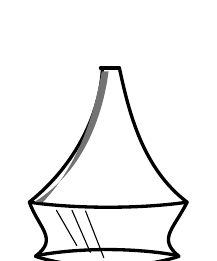
\begin{tikzpicture}[scale=0.86, line cap=round, line join=round]
  \draw[very thick] (-0.10,2.80) -- (0.18,2.80);
  \draw[very thick] (-0.07,2.80) .. controls (-0.10,2.15) and (-0.45,1.38) .. (-1.15,0.82);
  \draw[very thick] (0.18,2.80) .. controls (0.32,2.15) and (0.52,1.32) .. (1.18,0.82);
  \draw[very thick] (-1.15,0.82) .. controls (-1.00,0.42) and (-0.72,0.28) .. (-1.06,0.02);
  \draw[very thick] (1.18,0.82) .. controls (0.98,0.42) and (0.74,0.28) .. (1.06,0.02);
  \draw[very thick] (-1.06,0.02) .. controls (-0.45,-0.18) and (0.45,-0.18) .. (1.06,0.02);
  \draw[very thick] (-1.15,0.82) .. controls (-0.48,0.72) and (0.50,0.72) .. (1.18,0.82);
  \draw[very thick] (-1.05,0.03) .. controls (-0.42,0.15) and (0.42,0.15) .. (1.05,0.03);
  \fill[black!55] (-0.95,0.82) .. controls (-0.38,1.42) and (-0.18,2.20) .. (-0.08,2.75) -- (0.02,2.75) .. controls (-0.05,2.20) and (-0.30,1.30) .. (-1.08,0.82) -- cycle;
  \draw[thin] (-0.75,0.70)--(-0.45,0.18);
  \draw[thin] (-0.52,0.70)--(-0.25,0.08);
  \draw[thin] (-0.32,0.69)--(-0.05,0.00);
\end{tikzpicture}

{\footnotesize\bfseries Fig. 1.\({}^{\rm a}\) -- Pseudosphere.}
\end{center}

\emph{Case II. Elliptic type.} To obtain a real surface one must suppose
\[
 \frac{\lambda}{R}<1
\]
and, putting \(\lambda=R\sen\alpha\), the maximum value for \(\cosh\dfrac{u}{R}\) will be \(\dfrac1{\sen\alpha}\), and therefore the radius \(r\) of the parallel oscillates between
\[
 r=0
 \qquad\hbox{and}\qquad
 r=R\cos\alpha.
\]
When \(r=0\), \(\dfrac{dr}{du}=\sen\alpha\), and therefore all the meridians meet, at \(u=0\), the axis of rotation under the angle \(\alpha\); this point is a conical point of the surface.

The coordinates of a point of the meridian curve are expressed by elliptic functions of a parameter \(\tau\), with modulus \(k=\cos\alpha\). Indeed let us put
\[
 \senh\frac{u}{R}=\frac{k}{k'}\cn(\tau,k)
\]
and we shall have
\[
 r=Rk\cn\tau,
 \qquad
 z=Rk'\int_0^\tau \sn^2\tau\,d\tau
 =R\left\{\frac{H}{K}\tau-Z(\tau)\right\},
\]
where
\[
 Z(\tau)=\frac{\Theta'(\tau)}{\Theta(\tau)}
\]
is Jacobi's function and H, K are the known constants of the theory of elliptic functions. The portion of the curve from \(\tau=0\) to \(\tau=2K\) is represented in figure II); when \(\tau\) increases by \(4K\), the curve reproduces itself periodically. The corresponding surface of revolution consists of infinitely many congruent parts by translation along the axis; the maximum parallels of radius \(r=R\cos\alpha\) are cuspidal edges for the surface, because the points \(\tau=2mK\) (\(m\) integer) are cusps of the meridian.

\begin{center}
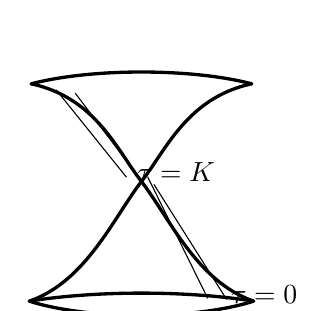
\begin{tikzpicture}[scale=0.8, line cap=round, line join=round]
  \draw[very thick] (-1.75,2.10) .. controls (-0.80,2.35) and (0.80,2.35) .. (1.75,2.10);
  \draw[very thick] (-1.75,2.10) .. controls (-0.72,1.88) and (-0.38,1.03) .. (0,0.55);
  \draw[very thick] (1.75,2.10) .. controls (0.72,1.88) and (0.38,1.03) .. (0,0.55);
  \draw[very thick] (0,0.55) .. controls (-0.44,-0.02) and (-0.88,-1.04) .. (-1.78,-1.35);
  \draw[very thick] (0,0.55) .. controls (0.44,-0.02) and (0.88,-1.04) .. (1.78,-1.35);
  \draw[very thick] (-1.78,-1.35) .. controls (-0.84,-1.65) and (0.84,-1.65) .. (1.78,-1.35);
  \draw[very thick] (-1.78,-1.35) .. controls (-0.72,-1.18) and (0.72,-1.18) .. (1.78,-1.35);
  \draw[thin] (-1.35,2.00)--(-0.24,0.62);
  \draw[thin] (-1.05,1.95)--(-0.12,0.72);
  \draw[thin] (1.35,-1.32)--(0.20,0.50);
  \draw[thin] (1.05,-1.30)--(0.10,0.62);
  \node at (0.55,0.70) {\(\tau=K\)};
  \node at (1.95,-1.25) {\(\tau=0\)};
\end{tikzpicture}

{\footnotesize\bfseries Fig. 2.\({}^{\rm a}\) -- Pseudospherical surface of revolution of elliptic type.}
\end{center}

\emph{Case III. Hyperbolic type.} In this case we have
\[
 r=\lambda\cosh\frac{u}{R},
 \qquad
 \frac{dr}{du}=\frac{\lambda}{R}\senh\frac{u}{R};
\]
the maximum value which \(u\) assumes in the real part of the curve corresponds to \(\senh\dfrac{u}{R}=\dfrac{R}{\lambda}\), and the radius of the parallel oscillates between the minimum \(\lambda\) and the maximum \(\sqrt{R^2+\lambda^2}\).

Putting here
\[
 \frac{R}{\sqrt{R^2+\lambda^2}}=k,
 \qquad
 \cosh\frac{u}{R}=\frac{\dn(\tau,k)}{k},
\]
we shall express the coordinates of a moving point on the curve by elliptic functions of the parameter \(\tau\), with the formulae
\[
 r=\frac{R}{k}\dn\tau,
 \qquad
 z=\frac{R}{k}\left\{\frac{H}{K}\tau-Z(\tau)\right\}.
\]
The form of the curve from \(\tau=0\) to \(\tau=2K\) is represented in figure 3.\({}^{\rm a}\); when \(\tau\) increases by \(2K\), the curve reproduces itself periodically. The maximum parallels corresponding to \(\tau=2mK\) (\(m\) integer) are cuspidal edges for the surface, and the minimum ones corresponding to \(\tau=(2m+1)K\) are geodesics.

\begin{center}
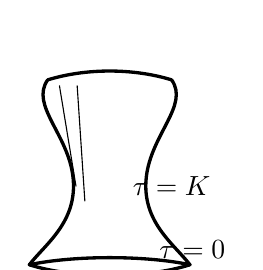
\begin{tikzpicture}[scale=0.75, line cap=round, line join=round]
  \draw[very thick] (-1.05,2.05) .. controls (-0.40,2.25) and (0.40,2.25) .. (1.05,2.05);
  \draw[very thick] (-1.05,2.05) .. controls (-1.35,1.62) and (-0.70,1.13) .. (-0.62,0.40)
                     .. controls (-0.54,-0.35) and (-1.08,-0.72) .. (-1.36,-1.08);
  \draw[very thick] (1.05,2.05) .. controls (1.35,1.62) and (0.70,1.13) .. (0.62,0.40)
                     .. controls (0.54,-0.35) and (1.08,-0.72) .. (1.36,-1.08);
  \draw[very thick] (-1.36,-1.08) .. controls (-0.62,-1.32) and (0.62,-1.32) .. (1.36,-1.08);
  \draw[very thick] (-1.36,-1.08) .. controls (-0.60,-0.92) and (0.60,-0.92) .. (1.36,-1.08);
  \draw[thin] (-0.85,1.95)--(-0.57,0.25);
  \draw[thin] (-0.55,1.95)--(-0.42,0.00);
  \node at (1.05,0.25) {\(\tau=K\)};
  \node at (1.40,-0.82) {\(\tau=0\)};
\end{tikzpicture}

{\footnotesize\bfseries Fig. 3.\({}^{\rm a}\) -- Pseudospherical surface of revolution of hyperbolic type.}
\end{center}

The three forms of pseudospherical surfaces of revolution just considered are distinct from one another, nor is it possible to apply one of them on another of a different species in such a way that parallels are laid on parallels. To ascertain this it is enough to observe that in the parabolic type the parallels have constant geodesic curvature \(\dfrac1R\), in the elliptic type the geodesic curvature of the parallels is \(>\dfrac1R\), and in the hyperbolic type instead \(<\dfrac1R\). Nevertheless, by the general theorem (§. 100), every pseudospherical surface of radius R is applicable on each of the surfaces I) II) III). Wishing to consider more closely this way of deforming every pseudospherical surface into a surface of revolution, we make the following observations:

a) On a pseudospherical surface S trace a horocycle and consider the geodesics orthogonal to it. By bending one will be able to give the surface the form of a pseudosphere, whose marked geodesics become the meridians.

b) On the pseudospherical surface S mark a point P and consider the geodesics issuing from P and the orthogonal geodesic circles; taking the parameters \(u,v\) as on pag. 224, we shall have
\[
 ds_1^2=du^2+R^2\senh^2\frac{u}{R}\,dv^2.
\]
Comparing with the linear element of the surface of revolution of elliptic type
\[
 ds_1^2=du_1^2+\lambda^2\senh^2\frac{u_1}{R}\,dv_1^2,
\]
we obtain for the formulae of applicability
\[
 u_1=u,
 \qquad
 \frac{\lambda}{R}v_1=v.
\]
It follows that when the longitude \(v_1\), on the surface of revolution II), is made to complete a whole revolution from 0 to \(2\pi\), the angle \(v\) runs through the interval from \(v=0\) to \(v=2\pi\sen\alpha<2\pi\). A portion of S around P is therefore enough to cover entirely one sheet of the surface II). Moreover the part of S beyond the geodesic circle of radius
\[
 u=\sett\cosh\left(\frac1{\sen\alpha}\right)
\]
has no correspondent on the surface (II); the portion of S around P to which one can give the form of a sheet of the surface II) is therefore bounded by a geodesic sector.

c) In the case of the surfaces III) of hyperbolic type, the minimum parallel is a geodesic and we can therefore apply any pseudospherical surface S on III) in such a way that an arbitrary geodesic \(g\) of S is laid on the minimum parallel. The part of S which is effectively applied on one sheet of III) is enclosed by a strip bounded by two lines geodesically parallel to \(g\) and equidistant from it, which after the deformation become the maximum parallels (cuspidal edges) of the zone. In the direction of the geodesic \(g\) the strip is then bounded by two geodesics orthogonal to \(g\), which join after the deformation into a single meridian of the zone. The length and breadth of the strip depend only on the radius one wishes to give to the minimum parallel.

\subsection*{\S. 104.\quad Surfaces with \(\infty^1\) applicability into themselves.}

The fundamental property of surfaces of constant curvature, which we proved in §. 100, can be stated by saying:

\emph{The linear element of every surface of constant curvature admits \(\infty^3\) transformations into itself.}

We now ask whether there exist other surfaces which admit continuous bendings into themselves. If these bendings constituted a double infinity, every point of the surface, by disposing of the two parameters of the transformation, could be transported into any other point (of a suitable region), and, by Gauss's theorem, the surface would be of constant curvature, and the supposed bendings would constitute a triple rather than a double infinity.

Now it is clear that every surface applicable on a surface of revolution admits a continuous bending into itself, corresponding to the rotation of the surface onto which it is applicable about the axis.

It is important to observe that the inverse theorem holds:

\emph{Every surface S which admits a continuous bending into itself is applicable on a surface of revolution.} In substance this theorem already follows from the discussion in §. 99, because there it was seen that the formulae of applicability of two surfaces S, S' can contain an arbitrary parameter only in the case in which S, S' are applicable on the same surface of revolution. But we can prove the property anew by the following geometrical considerations. If S has constant curvature, the theorem has already been proved by the investigations of the preceding numbers. In the contrary case, during the supposed continuous bending, the lines L of equal curvature
\[
 K=\hbox{constant}
\]
must, by Gauss's theorem, slide upon themselves. And since such a bending depends on a parameter varying continuously, every point of a line L can be transported into any other point of the same line; hence it follows that the lines L have constant geodesic curvature. Moreover the lines geodesically parallel to a line L, during the said bending, also evidently slide upon themselves. From these considerations the stated theorem follows easily, and indeed the following property holds:

\emph{If a surface S possesses a system of lines L geodesically parallel and of constant geodesic curvature, it is applicable on a surface of revolution whose parallels are the deforms of the lines L.}

Indeed take as coordinate system the one formed by the lines L (\(u=\) constant) and by the orthogonal geodesics (\(v=\) constant); the linear element will take the form
\[
 ds^2=du^2+G\,dv^2.
\]
Now, by hypothesis,
\[
 -\frac1{\rho_u}=\frac{\partial\log\sqrt G}{\partial u}=\varphi(u),
\]
whence
\[
 \sqrt G=UV,
\]
where U is a function of \(u\) and V of \(v\). Putting
\[
 \int V\,dv=v_1,
\]
one displays the linear element
\[
 ds^2=du^2+U^2\,dv_1^2
\]
of a surface of revolution.

\subsection*{\S. 105.\quad Applicable surfaces of revolution.}

We now consider some simple examples of applicable surfaces, and first we seek whether two surfaces of revolution S, S\(_1\) can be applicable one on the other.

From Gauss's theorem it follows first that the parallels of S will be laid on the parallels of S\(_1\), and hence the meridians also on the meridians. Naturally surfaces of constant curvature are exceptional, but the following considerations also hold for these surfaces, when one adds the condition that the parallels of one are laid on the parallels of the other.

If the linear element of S is given by
\[
 ds^2=du^2+r^2\,dv^2
\]
and that of S\(_1\) by
\[
 ds_1^2=du_1^2+r_1^2\,dv_1^2,
\]
we may at once put \(u_1=u\), counting the meridian arcs from two corresponding parallels. To transform the two linear elements one into the other, it will be necessary to put \(v_1=v_1(v)\), determining this function from the condition
\[
 r_1(u)\frac{dv_1}{dv}=r(u).
\]
It follows that
\[
 r_1=kr,
 \qquad
 v_1=\frac{v}{k}\quad (k\hbox{ arbitrary constant}).
\]
If therefore \(r=\varphi(u)\) is the equation of the meridian of S, the coordinates of the meridian of S\(_1\) will be given by
\[
 r=k\varphi(u),
 \qquad
 z=\int\sqrt{1-k^2\varphi'^2(u)}\,du.
\]
It follows: \emph{Every surface of revolution can be deformed in \(\infty^1\) ways, while remaining a surface of revolution.}

Let us consider more closely the way in which S\(_1\) is applied on S. If we suppose \(k<1\), the formula
\[
 v=kv_1
\]
shows that when the longitude \(v_1\) has completed a whole revolution on S\(_1\), becoming equal to \(2\pi\), the longitude \(v\) becomes
\[
 v=2k\pi<2\pi.
\]
Therefore, applying S\(_1\) on S, the latter is not entirely covered, but a portion (lune) is missing, bounded by two meridians whose planes make an angle of magnitude equal to \(2\pi(1-k)\). To lay S\(_1\) on S it is therefore convenient to cut S\(_1\) along a meridian and open it by deforming it so that the edges of the cut become on S two distinct meridians. If one observes that the geodesic curvature of the parallels and the total curvature of the surface do not vary in the deformation, one will see at once that at two corresponding points the curvature of the meridian of S exceeds that of the meridian of S\(_1\).

The case \(k>1\) evidently corresponds to the inverse deformation of S into S\(_1\), for which it is convenient to remove a lune from S, then restoring the continuity of the surface by joining into one, by deformation, the two meridians of the removed lune. It should also be observed that to a point of the meridian of S there corresponds a real point of the meridian of S\(_1\) so long as \(k\dfrac{dr}{du}<1\), which always happens if \(k<1\). But when \(k>1\), the parallels to which the value \(\dfrac1k\) of \(\dfrac{dr}{du}\) corresponds bound on S a zone, which is the portion of S effectively applicable on S\(_1\). After the deformation, the extreme parallels of this zone become cuspidal parallels for S\(_1\).

As an example, let us consider the deformations of surfaces of revolution of constant curvature.

a) For the sphere of radius \emph{one} one may take
\[
 r=\cos u
\]
and the coordinates of the deformed meridians are given by the formulae
\[
 r=k\cos u,
 \qquad
 z=\int\sqrt{1-k^2\sen^2 u}\,du.
\]
We can express them by elliptic functions of a parameter \(\tau\). Thus, if \(k<1\), we put \(\cos u=\cn(\tau,k)\) and shall have
\[
 r=k\cn\tau,
 \qquad
 z=\left(1-\frac{H}{K}\right)\tau+Z(\tau);
\]
if \(k>1\) we change \(k\) into \(\dfrac1k\) and, putting
\[
 \cos u=\dn(\tau,k)
\]
we shall have
\[
 r=\frac{\dn\tau}{k},
 \qquad
 z=\left(k-\frac{H}{Kk}\right)\tau+\frac1k Z(\tau).
\]
In the case \(k<1\), one will obtain a spindle-shaped surface, whose meridians meet the axis at a point (conical for the surface) under the angle \(\alpha=\arc\sen k\). In the case \(k>1\) one has a zone bounded by two minimum cuspidal parallels. The following three figures represent precisely the surfaces corresponding to the three cases. On the middle one, the sphere, the zone which is applied on the surface of fig. 6.\({}^{\rm a}\) is marked.

\begin{center}
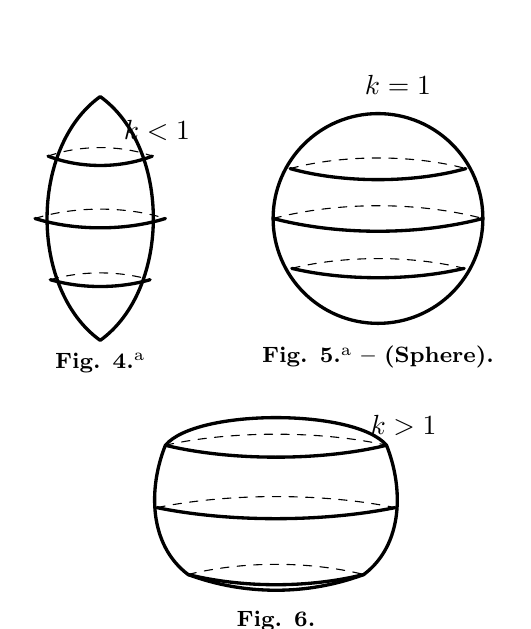
\begin{tikzpicture}[scale=0.72, line cap=round, line join=round]
  \begin{scope}[xshift=-3.7cm]
    \draw[very thick] (0,2.15) .. controls (-1.25,1.25) and (-1.25,-1.25) .. (0,-2.15)
                      .. controls (1.25,-1.25) and (1.25,1.25) .. (0,2.15);
    \draw[very thick] (-0.92,1.10) .. controls (-0.35,0.88) and (0.35,0.88) .. (0.92,1.10);
    \draw[dashed] (-0.92,1.10) .. controls (-0.35,1.30) and (0.35,1.30) .. (0.92,1.10);
    \draw[very thick] (-1.15,0.00) .. controls (-0.45,-0.22) and (0.45,-0.22) .. (1.15,0.00);
    \draw[dashed] (-1.15,0.00) .. controls (-0.45,0.22) and (0.45,0.22) .. (1.15,0.00);
    \draw[very thick] (-0.88,-1.08) .. controls (-0.32,-1.24) and (0.32,-1.24) .. (0.88,-1.08);
    \draw[dashed] (-0.88,-1.08) .. controls (-0.32,-0.92) and (0.32,-0.92) .. (0.88,-1.08);
    \node at (1.00,1.55) {\(k<1\)};
    \node at (0,-2.55) {\footnotesize\bfseries Fig. 4.\({}^{\rm a}\)};
  \end{scope}
  \begin{scope}[xshift=1.2cm]
    \draw[very thick] (0,0) circle (1.85);
    \draw[very thick] (-1.55,0.88) .. controls (-0.62,0.62) and (0.62,0.62) .. (1.55,0.88);
    \draw[dashed] (-1.55,0.88) .. controls (-0.62,1.13) and (0.62,1.13) .. (1.55,0.88);
    \draw[very thick] (-1.85,0.0) .. controls (-0.70,-0.30) and (0.70,-0.30) .. (1.85,0.0);
    \draw[dashed] (-1.85,0.0) .. controls (-0.70,0.30) and (0.70,0.30) .. (1.85,0.0);
    \draw[very thick] (-1.52,-0.88) .. controls (-0.60,-1.10) and (0.60,-1.10) .. (1.52,-0.88);
    \draw[dashed] (-1.52,-0.88) .. controls (-0.60,-0.65) and (0.60,-0.65) .. (1.52,-0.88);
    \node at (0.35,2.35) {\(k=1\)};
    \node at (0,-2.45) {\footnotesize\bfseries Fig. 5.\({}^{\rm a}\) -- (Sphere).};
  \end{scope}
  \begin{scope}[xshift=-0.6cm,yshift=-5.1cm]
    \draw[very thick] (-1.95,1.10) .. controls (-1.40,1.75) and (1.40,1.75) .. (1.95,1.10)
                      .. controls (2.25,0.35) and (2.25,-0.65) .. (1.55,-1.18)
                      .. controls (0.55,-1.55) and (-0.55,-1.55) .. (-1.55,-1.18)
                      .. controls (-2.25,-0.65) and (-2.25,0.35) .. (-1.95,1.10);
    \draw[very thick] (-1.95,1.10) .. controls (-0.80,0.82) and (0.80,0.82) .. (1.95,1.10);
    \draw[dashed] (-1.95,1.10) .. controls (-0.80,1.36) and (0.80,1.36) .. (1.95,1.10);
    \draw[very thick] (-2.10,0.00) .. controls (-0.82,-0.26) and (0.82,-0.26) .. (2.10,0.00);
    \draw[dashed] (-2.10,0.00) .. controls (-0.82,0.26) and (0.82,0.26) .. (2.10,0.00);
    \draw[very thick] (-1.55,-1.18) .. controls (-0.58,-1.42) and (0.58,-1.42) .. (1.55,-1.18);
    \draw[dashed] (-1.55,-1.18) .. controls (-0.58,-0.94) and (0.58,-0.94) .. (1.55,-1.18);
    \node at (2.25,1.45) {\(k>1\)};
    \node at (0,-2.00) {\footnotesize\bfseries Fig. 6.};
  \end{scope}
\end{tikzpicture}
\end{center}

b) The pseudosphere enjoys the singular property that all its deforms of revolution coincide with the pseudosphere itself, as follows from the observation that the geodesic curvature of the parallels is constant \(=\dfrac1R\).

In the case of contraction of the parallels (\(k<1\)), the maximum parallel (cuspidal edge) becomes a smaller parallel, and the zone comprised between this parallel and the maximum one thus remains uncovered. In the inverse deformation a smaller parallel becomes the cuspidal parallel; but to effect this deformation one must first cut from the pseudosphere the zone comprised between this parallel and the present cuspidal parallel.

The deformation of the other two classes of pseudospherical surfaces of revolution leads to surfaces of the same type, varying in the case of surfaces of elliptic type the angle of aperture at the vertex (conical point), and for those of hyperbolic type the radius of the minimum parallel.

\subsection*{\S. 106.\quad Helicoids and Bour's theorem.}

The result of §. 104 permits an immediate application to an important class of surfaces, called \emph{helicoids}. These are the surfaces generated by a plane or double-curvature curve endowed, about an axis and parallel to it, with a double rotational and translational motion, the ratio of whose velocities is constant. The various points of the generating curve describe as many circular helices, having the axis of the helicoid as common axis and all of the same pitch. If we observe that the helicoidal motion by which the surface has been generated makes the whole surface slide over itself, it will suffice to apply the theorem of §. 105 to obtain the elegant result due to Bour:

\emph{Every helicoid is applicable on a surface of revolution; the helices are laid on the parallels.}

It is clear that the surface of revolution is covered infinitely many times by the helicoid, every helix winding infinitely many times around the corresponding parallel.

We now give a direct proof of this theorem, to find also the effective formulae of applicability. For this purpose observe that by passing a plane through the axis one produces a section in the helicoid, and if this section (\emph{meridian profile}) is given about the axis the helicoidal motion which generated the surface, the section itself will describe the helicoid. A helicoid is determined when its meridian profile and the parameter of the helicoidal motion are assigned.

Taking as axis of \(z\) the axis of the helicoid, and denoting by \(\rho\) the distance of a point of the meridian profile from the axis, let
\[
 z=\varphi(\rho)
\]
be the equation of the meridian profile. Then let \(v\) denote the angle through which, after any time whatever, the plane of the meridian profile has rotated, and let \(m\)
the ratio of the velocity of translation to that of rotation. The coordinates \(x,y,z\) of a moving point on the helicoid will be given as functions of \(\rho,v\) by the formulae
\[
 x=\rho\cos v,
 \qquad y=\rho\sen v,
 \qquad z=\varphi(\rho)+mv,
\]
whence
\[
 ds^2=\{1+\varphi'^2(\rho)\}\,d\rho^2+2m\varphi'(\rho)\,d\rho\,dv+(\rho^2+m^2)\,dv^2.
\]
We change the coordinate lines \(v\), putting
\[
 v=kv_1-m\int\frac{\varphi'(\rho)\,d\rho}{\rho^2+m^2},
\]
where \(k\) is an arbitrary constant, and there will result
\[
 ds^2=\left\{1+\frac{\rho^2\varphi'^2(\rho)}{\rho^2+m^2}\right\}d\rho^2+k^2(\rho^2+m^2)\,dv_1^2.
\]
Comparing this linear element with that
\[
 ds_1^2=\{1+\psi'^2(r)\}\,dr^2+r^2dv_1^2
\]
of a surface of revolution, whose meridian curve has equation
\[
 z=\psi(r),
\]
we can identify them by putting between \(r,\psi(r),\rho,\varphi(\rho)\) the relations
\begin{equation}\tag{8}
\left\{
\begin{aligned}
 r^2&=k^2(\rho^2+m^2),\\
 \{1+\psi'^2(r)\}\left(\frac{dr}{d\rho}\right)^2
 &=1+\frac{\rho^2\varphi'^2(\rho)}{\rho^2+m^2}.
\end{aligned}
\right.
\end{equation}
These formulae again prove Bour's theorem; moreover one sees that, once a helicoid or a surface of revolution is chosen arbitrarily, one can find by quadratures the surfaces of revolution or the helicoids on which they are applicable. In the first case, by eliminating \(\rho\), one will in fact have \(\psi'(r)\), and in the second, by eliminating \(r\), one will obtain \(\varphi'(\rho)\).

\subsection*{\S. 107.\quad The ruled helicoid of minimum area and the ruled hyperboloid.}

Let us apply formulae (8) to two simple examples.

\(1.^\circ\) Let the meridian profile be a straight line perpendicular to the axis; the helicoid generated is \emph{the ruled helicoid of minimum area} already considered in \S. 24 c. I. Then in (8) we shall have \(\varphi'(\rho)=0\), hence
\[
 1+\psi'^2(r)=\left(\frac{d\rho}{dr}\right)^2=\frac{r^2}{k^2(r^2-m^2k^2)}
\]
and, taking the arbitrary constant \(k=1\), there will result
\[
 z=\psi(r)=m\int\frac{dr}{\sqrt{r^2-m^2}}
\]
and, carrying out the quadrature,
\[
 r=m\cosh\frac{z}{m}.
\]
The meridian curve is therefore an ordinary catenary, having the axis of revolution as directrix.

The corresponding surface of revolution is called the \emph{catenoid}. The generators of the helicoid are laid on the meridians and the axis \(\rho=0\) becomes the throat circle \(r=m\) of the catenoid.

\(2.^\circ\) Let the meridian profile be a straight line inclined to the axis by an angle \(\alpha\); its equation will be
\[
 z=\rho\cot\alpha
\]
and putting in (8)
\[
 \varphi'(\rho)=\cot\alpha,
\]
there will result
\[
 1+\psi'^2(r)=\left\{1+\frac{(r^2-k^2m^2)\cot^2\alpha}{r^2}\right\}
 \frac{r^2}{k^2(r^2-k^2m^2)}
\]
and, putting
\[
 k=\cot\alpha,
\]
we shall have
\[
 \psi'(r)=\frac{\tg\alpha\,r}{\sqrt{r^2-m^2\cot^2\alpha}}.
\]
The equation of the meridian of the surface of revolution is therefore
\[
 z=\tg\alpha\sqrt{r^2-m^2\cot^2\alpha},
\]
that is,
\[
 \frac{r^2}{m^2\cot^2\alpha}-\frac{z^2}{m^2}=1.
\]
The surface of revolution is thus a hyperboloid of revolution of one sheet. One easily sees that the axis \(\rho=0\) of the helicoid is laid on the throat circle of the hyperboloid and the generators of the helicoid on the generators of one system of the hyperboloid.

\subsection*{\S. 108.\quad The second problem of applicability.}

We now pass to the second and more important problem of the theory of applicability, which would consist in: \emph{Finding all the surfaces applicable on a given surface}, or else: \emph{Finding all the surfaces with assigned linear element}.

This difficult problem is known how to be solved completely only in a few special cases, which will be considered later in this treatise. However, the general theorems on partial differential equations make it possible to establish very important general results relative to the problem just stated. It is precisely with these that we now wish to concern ourselves, so far as the limits of brevity which we have imposed on ourselves allow\srcfn{1}{The reader will find in volume III of Darboux's lectures, p. 263 ff., a complete treatment of the problem.}.

A first way of treating the present problem follows naturally from the fundamental formulae of the theory of surfaces (chap. IV). Once the first fundamental form is assigned,
\[
 E\,du^2+2F\,du\,dv+G\,dv^2,
\]
to every surface with the given linear element there will correspond a second fundamental form
\[
 D\,du^2+2D'\,du\,dv+D''\,dv^2,
\]
and the functions \(D,D',D''\) must satisfy equations (III), (IV) \S. 56 (p. 119), namely Gauss's equation and the two equations of Codazzi. Conversely, if \(D,D',D''\) are three functions of \(u,v\) satisfying the three equations just cited, there exists a corresponding surface with the assigned linear element, and its effective determination depends further on a Riccati equation.

Thus, for example, if we took the linear element of a surface of revolution
\[
 ds^2=du^2+r^2dv^2,
\]
we could satisfy the cited fundamental equations by taking \(D,D',D''\) to be functions of \(u\) alone. The surfaces applicable on the surfaces of revolution which would thereby be found are precisely the helicoids of \S. 106\srcfn{1}{To prove it, it suffices to observe that in this case both the first and the second fundamental forms admit the continuous transformation into themselves:
\[
 u'=u,\qquad v'=v+\hbox{constant}
\]
and therefore the surface, admitting a continuous motion into itself, is a helicoid.}.

\subsection*{\S. 109.\quad Partial differential equation for the second problem.}

Far more important than the preceding method is the one which we now pass to expound, basing ourselves on the result obtained in \S. 69, and precisely on equation (B), p. 146.

For every surface
\[
 x=x(u,v),\qquad y=y(u,v),\qquad z=z(u,v)
\]
with assigned linear element
\begin{equation}\tag{9}
 dx^2+dy^2+dz^2=E\,du^2+2F\,du\,dv+G\,dv^2
\end{equation}
the equation just recalled teaches that each of the three unknown functions \(x,y,z\) satisfies the partial differential equation of the second order
\begin{equation}\tag{10}
 \Delta_{22}x=(1-\Delta_1x)K,
\end{equation}
whose coefficients are precisely formed with \(E,F,G\) and their first and second derivatives\srcfn{2}{If, using Monge's notation, one denotes by \(p,q;r,s,t\) the first and second derivatives of the unknown function, the equation is written
\[
\begin{aligned}
&\left(r-\chr{1}{1}{1}p-\chr{1}{1}{2}q\right)
 \left(t-\chr{2}{2}{1}p-\chr{2}{2}{2}q\right)
-\left(s-\chr{1}{2}{1}p-\chr{1}{2}{2}q\right)^2 \\
&\hspace{3em}=K\left\{EG-F^2-\left[E q^2-2Fpq+G p^2\right]\right\}
\end{aligned}
\]
and it has Ampère's linear form with respect to \(rt-s^2\), \(r,s,t\).}.

Now it is important to observe with Darboux that equation (10) has the following meaning:
\begin{center}
\emph{If \(x(u,v)\) is a solution of it, the quadratic form}
\end{center}
\[
\begin{aligned}
&E\,du^2+2F\,du\,dv+G\,dv^2-dx^2 \\
&=\left\{E-\left(\frac{\partial x}{\partial u}\right)^2\right\}du^2
+2\left\{F-\frac{\partial x}{\partial u}\frac{\partial x}{\partial v}\right\}du\,dv
+\left\{G-\left(\frac{\partial x}{\partial v}\right)^2\right\}dv^2
\end{aligned}
\]
\begin{center}
\emph{will have zero curvature.}
\end{center}
To prove this in the simplest way, put
\[
 x=u,
 \qquad F=0,
\]
which is evidently legitimate by the invariant property of our equation. Then (10) becomes
\[
 \chr{1}{1}{1}\chr{2}{2}{1}-\chr{1}{2}{1}^2=G(E-1)K
\]
and, substituting for Christoffel's symbols their present values
\[
 \chr{1}{1}{1}=\frac1{2E}\frac{\partial E}{\partial u},\qquad
 \chr{1}{2}{1}=\frac1{2E}\frac{\partial E}{\partial v},\qquad
 \chr{2}{2}{1}=-\frac1{2E}\frac{\partial G}{\partial u},
\]
one obtains
\[
 \frac{\partial E}{\partial u}\frac{\partial G}{\partial u}
 +\left(\frac{\partial E}{\partial v}\right)^2
 +4E^2G(E-1)K=0.
\]
Now in orthogonal coordinates one has (\S. 43, p. 93):
\begin{equation}\tag{11}
\begin{aligned}
4E^2G^2K={}&E\left[\frac{\partial E}{\partial v}\frac{\partial G}{\partial v}+
\left(\frac{\partial G}{\partial u}\right)^2\right]
+G\left[\frac{\partial E}{\partial u}\frac{\partial G}{\partial u}+
\left(\frac{\partial E}{\partial v}\right)^2\right]\\
&-2EG\left[\frac{\partial^2E}{\partial v^2}+\frac{\partial^2G}{\partial u^2}\right]
\end{aligned}
\end{equation}
and the preceding equation, multiplied by \(G\), is written
\[
\begin{aligned}
&G\left[\frac{\partial E}{\partial u}\frac{\partial G}{\partial u}+
\left(\frac{\partial E}{\partial v}\right)^2\right]
+E(E-1)\left[\frac{\partial E}{\partial v}\frac{\partial G}{\partial v}+
\left(\frac{\partial G}{\partial u}\right)^2\right] \\
&\quad+G(E-1)\left[\frac{\partial E}{\partial u}\frac{\partial G}{\partial u}+
\left(\frac{\partial E}{\partial v}\right)^2\right]
-2EG(E-1)\left(\frac{\partial^2E}{\partial v^2}+\frac{\partial^2G}{\partial u^2}\right)=0.
\end{aligned}
\]
Suppressing the terms which cancel and dividing by \(E\), one obtains the equivalent equation
\[
\begin{aligned}
&(E-1)\left[\frac{\partial E}{\partial v}\frac{\partial G}{\partial v}+
\left(\frac{\partial G}{\partial u}\right)^2\right]
+G\left[\frac{\partial G}{\partial u}\frac{\partial E}{\partial u}+
\left(\frac{\partial E}{\partial v}\right)^2\right]\\
&\qquad -2(E-1)G\left[\frac{\partial^2E}{\partial v^2}+\frac{\partial^2G}{\partial u^2}\right]=0,
\end{aligned}
\]
which, according to (11) itself, expresses precisely that the form
\[
 (E-1)du^2+Gdv^2
\]
has zero curvature.

This being premised, let us suppose that we know a solution \(x(u,v)\) of equation (10), and let us see whether there will exist a real surface corresponding to the assigned linear element. The differential form
\begin{equation}\tag{12}
 E\,du^2+2F\,du\,dv+G\,dv^2-dx^2
\end{equation}
then having zero curvature, in order that there exist two other real functions \(y(u,v),z(u,v)\) satisfying (9), it is necessary and sufficient that (12) be a definite form, that is, that one have
\[
\left[E-\left(\frac{\partial x}{\partial u}\right)^2\right]
\left[G-\left(\frac{\partial x}{\partial v}\right)^2\right]
-\left[F-\frac{\partial x}{\partial u}\frac{\partial x}{\partial v}\right]^2>0,
\]
or
\[
 \Delta_1x<1.
\]
Supposing this condition satisfied, one will have \(y,z\) by quadratures (\S\S. 37 and 93); and manifestly \(y,z\) will be determined up to a transformation of coordinates.

Thus: \emph{To every real solution \(x(u,v)\) of equation (10), which also satisfies the inequality \(\Delta_1x<1\), there corresponds one and only one real surface with the assigned linear element. Once this solution is known, the corresponding surface will be obtained by quadratures.}

\subsection*{\S. 110.\quad Indeformability of surfaces with a rigid line.}

Let us now deal with the following question: \emph{Given a surface S and a curve \(\Gamma\) traced on it, can the surface be bent without deforming the curve?}

Under the affirmative hypothesis, let \(S_1\) be one of the forms assumed by S by bending, while \(\Gamma\) remains rigid: we may suppose the configuration \(S_1\) of S so near to the initial one that the normals to \(S_1\), S along \(\Gamma\) are as near to one another as desired. But then, if one observes that \(\Gamma\) will have the same geodesic curvature on \(S_1\) and S, and recalls the relation linking geodesic curvature with absolute curvature (\S. 84), one will immediately conclude that along \(\Gamma\) the normals to \(S_1\), S coincide.

For simplicity let us now take on S (and \(S_1\)) an orthogonal coordinate system \((u,v)\), and let
\[
 v=0
\]
be the equation of the curve \(\Gamma\). We denote by appending the index 1 the quantities relative to \(S_1\), and we shall evidently have:
\[
\left.
\begin{gathered}
 x_1=x,
 \quad y_1=y,
 \quad z_1=z,\\
 \frac{\partial x_1}{\partial u}=\frac{\partial x}{\partial u},\quad
 \frac{\partial y_1}{\partial u}=\frac{\partial y}{\partial u},\quad
 \frac{\partial z_1}{\partial u}=\frac{\partial z}{\partial u},\\
 \frac{\partial x_1}{\partial v}=\frac{\partial x}{\partial v},\quad
 \frac{\partial y_1}{\partial v}=\frac{\partial y}{\partial v},\quad
 \frac{\partial z_1}{\partial v}=\frac{\partial z}{\partial v},\\
 X_1=X,
 \quad Y_1=Y,
 \quad Z_1=Z
\end{gathered}
\right\}\quad \hbox{for }v=0.
\]
Now, if we consider for example \(x_1,x\), they are solutions of the same partial differential equation of the second order (10), and they coincide in their values and in those of their first derivatives for \(v=0\). If we prove that \emph{also the three second derivatives of \(x_1\) coincide with the corresponding ones of \(x\) for \(v=0\)}, then, by the general theorems on the solutions of partial differential equations\srcfn{1}{Cf. for example \textsc{Goursat}. -- \emph{Leçons sur l'intégration des équations aux dérivées partielles du premier ordre}, p.\textsuperscript{e} 22.}, it will be proved that \(x_1,x\) coincide for all values of \(u,v\). The same being repeatable for \(y_1,y;z_1,z\), it will follow that \(S_1,S\) coincide. Now from the initial conditions
\[
 \frac{\partial x_1}{\partial u}=\frac{\partial x}{\partial u},
 \qquad
 \frac{\partial x_1}{\partial v}=\frac{\partial x}{\partial v},
 \quad \hbox{for }v=0
\]
there follows at once
\[
 \frac{\partial^2x_1}{\partial u^2}=\frac{\partial^2x}{\partial u^2},
 \qquad
 \frac{\partial^2x_1}{\partial u\partial v}=\frac{\partial^2x}{\partial u\partial v},
 \quad \hbox{for }v=0.
\]
The fundamental formulae (I) \S. 55, p. 116, of the theory of surfaces consequently show that one has
\[
 D_1=D,
 \qquad D'_1=D',
 \quad \hbox{for }v=0.
\]
The equality
\[
 DD''-D'^2=D_1D''_1-D_1'^2,
\]
therefore gives, after putting \(v=0\),
\[
 DD''=DD''_1,
 \quad \hbox{for }v=0.
\]
It follows that
\[
 (D''_1)_{v=0}=(D'')_{v=0},
\]
\emph{unless} \((D)_{v=0}=0\). Excluding this case, from the third of the cited formulae (I) \S. 55 there follows precisely, as was to be proved,
\[
 \frac{\partial^2x_1}{\partial v^2}=\frac{\partial^2x}{\partial v^2},
 \quad \hbox{for }v=0,
\]
and hence \(S_1,S\) coincide.

In the excluded case, \((D)_{v=0}=0\), the line \(v=0\) is an asymptotic line of S; we can therefore state the theorem: \emph{If on a flexible surface S a curve \(\Gamma\) is kept rigid, the surface cannot be deformed, unless the curve \(\Gamma\) is an asymptotic line of S.}

In the case where the line \(\Gamma\) is an asymptotic line, further properties of partial differential equations, which can only be mentioned here, show that it is indeed possible to deform the surface without deforming the curve. This is a singular property of the asymptotic lines, for which they are also called \emph{lines of bending}. This property, which distinguishes them from every other line of the surface, depends properly on the fact that: On every surface S the asymptotic lines are the \emph{characteristics} of the partial differential equation (10), on which the deformation of S depends\srcfn{1}{Writing (10) in the form
\[
 \Phi(r,s,t)=0
\]
of the note to the preceding number, the differential equation of the characteristics
\[
 \frac{\partial\Phi}{\partial t}\,du^2-\frac{\partial\Phi}{\partial s}\,du\,dv+\frac{\partial\Phi}{\partial r}\,dv^2=0,
\]
by (I) \S. 55 becomes precisely the differential equation of the asymptotics
\[
 D\,du^2+2D'\,du\,dv+D''\,dv^2=0
\]
(Cf. \textsc{Darboux}, t. III, p. 252).}.

\subsection*{\S. 111.\quad Deformation of the surface with assigned deform of a curve.}

The theorem just proved makes natural the question: \emph{Is it possible to deform a surface \(S'\) in such a way that an assigned curve C on it assumes a preassigned form \(\Gamma\)?}

We observe first that, if the deformation sought is possible, the absolute curvature of \(\Gamma\) must at every point be greater than, or at most equal to, the geodesic curvature of C at the corresponding point. Suppose this condition satisfied, and indeed for the moment exclude the case of equality of the absolute and geodesic curvature of \(\Gamma\), since then \(\Gamma\) would be asymptotic on the deformed surface.

Under the hypothesis that the required deformation exists, let S be the deformed surface, on which we take an orthogonal coordinate system \((u,v)\) as in the preceding number, such that the curve \(\Gamma\) is \(v=0\). For greater clarity we also fix that the parameter \(u\) be the arc of \(\Gamma\), counted from one of its fixed points, so that we shall have
\[
 E=1,
 \quad \hbox{for }v=0.
\]
Let \(\sigma\) denote the angle through which, in the positive sense, in the normal plane to \(\Gamma\), the positive direction of the normal to S must rotate in order to be superposed on that of the principal normal of \(\Gamma\). Retaining for the curve \(\Gamma\) the usual notation of the theory of curves (chap. I), we shall thus have, for \(v=0\):
\begin{equation}\tag{13}
\left\{
\begin{aligned}
\alpha&=\frac{\partial x}{\partial u},
&\beta&=\frac{\partial y}{\partial u},
&\gamma&=\frac{\partial z}{\partial u},\\
\xi&=\cos\sigma\,X-\sen\sigma\,\frac1{\sqrt G}\frac{\partial x}{\partial v},
&\eta&=\cos\sigma\,Y-\sen\sigma\,\frac1{\sqrt G}\frac{\partial y}{\partial v},\\
\zeta&=\cos\sigma\,Z-\sen\sigma\,\frac1{\sqrt G}\frac{\partial z}{\partial v},\\
\lambda&=-\cos\sigma\,\frac1{\sqrt G}\frac{\partial x}{\partial v}-\sen\sigma\,X,
&\mu&=-\cos\sigma\,\frac1{\sqrt G}\frac{\partial y}{\partial v}-\sen\sigma\,Y,\\
\nu&=-\cos\sigma\,\frac1{\sqrt G}\frac{\partial z}{\partial v}-\sen\sigma\,Z.
\end{aligned}
\right.
\end{equation}
Now one has
\[
 \frac{\partial^2x}{\partial u^2}=\chr{1}{1}{1}\frac{\partial x}{\partial u}+
 \chr{1}{1}{2}\frac{\partial x}{\partial v}+DX=\frac{\xi}{\rho}
\]
with the analogous formulae for \(y,z\), and since
\begin{equation}\tag{14}
 \chr{1}{1}{1}_{v=0}=\left(\frac1{2E}\frac{\partial E}{\partial u}\right)_{v=0}=0,
 \qquad
 \chr{1}{1}{2}_{v=0}=-\frac1{2G}\frac{\partial E}{\partial v}=\left(\frac1{\rho_v}\right)_{v=0}-\frac1{\sqrt G},
\end{equation}
from comparison with (13) we deduce
\begin{equation}\tag{15}
 D=\frac{\cos\sigma}{\rho},
 \qquad
 \frac1{\rho_v}=-\frac{\sen\sigma}{\rho}.
\end{equation}
The second of these, since the absolute curvature \(\dfrac1\rho\) and the geodesic curvature \(\dfrac1{\rho_v}\) of \(\Gamma\) are known, gives for the unknown angle \(\sigma\) two supplementary values.

Let one of these two values be taken for \(\sigma\); each of them will effectively lead to a corresponding surface S\srcfn{1}{That the proposed problem should in this way have two different solutions does not contradict the theorem of \S. 110, since the two surfaces S thereby obtained are indeed applicable to one another, and the curve \(\Gamma\), in the continuous deformation of one surface into the other, indeed finally resumes the form that it had at the beginning, but changes form in the intermediate states.}, and from (13) for the initial values (for \(v=0\)) of \(\dfrac{\partial x}{\partial v},\dfrac{\partial y}{\partial v},\dfrac{\partial z}{\partial v}\) we shall have:
\begin{equation}\tag{16}
\left\{
\begin{aligned}
\frac{\partial x}{\partial v}&=-\sqrt G(\xi\sen\sigma+\lambda\cos\sigma),\\
\frac{\partial y}{\partial v}&=-\sqrt G(\eta\sen\sigma+\mu\cos\sigma),\\
\frac{\partial z}{\partial v}&=-\sqrt G(\zeta\sen\sigma+\nu\cos\sigma).
\end{aligned}
\right.
\end{equation}
It will also be useful to note the values of \(X,Y,Z\) along \(\Gamma\), which are
\begin{equation}\tag{11*}
\left\{
\begin{aligned}
X&=\xi\cos\sigma-\lambda\sen\sigma,\\
Y&=\eta\cos\sigma-\mu\sen\sigma,\\
Z&=\zeta\cos\sigma-\nu\sen\sigma.
\end{aligned}
\right.
\end{equation}
It follows that for these three solutions of equation (10)
\[
 \Delta_{22}\theta=(1-\Delta_1\theta)K
\]
we shall also know the initial values (for \(v=0\)) of the functions themselves and of the second partial derivatives
\[
 \frac{\partial^2x}{\partial u^2},\quad
 \frac{\partial^2x}{\partial u\partial v},\quad
 \frac{\partial^2y}{\partial u^2},\quad
 \frac{\partial^2y}{\partial u\partial v},\quad
 \frac{\partial^2z}{\partial u^2},\quad
 \frac{\partial^2z}{\partial u\partial v},
\]
The partial differential equation (10), which they satisfy, will then furnish \emph{at least for one} of them the values of the second derivatives
\[
 \frac{\partial^2x}{\partial v^2},\quad
 \frac{\partial^2y}{\partial v^2},\quad
 \frac{\partial^2z}{\partial v^2},
\]
since otherwise, for \(v=0\), the expression
\[
 \frac{\partial^2x}{\partial u^2}-\chr{1}{1}{1}\frac{\partial x}{\partial u}-\chr{1}{1}{2}\frac{\partial x}{\partial v},
\]
with the two analogous expressions for \(y,z\), would have to vanish. But these, with substitution of the initial values and taking account of the second of (15), become
\[
\frac{\cos\sigma}{\rho}(\xi\cos\sigma-\lambda\sen\sigma),\quad
\frac{\cos\sigma}{\rho}(\eta\cos\sigma-\mu\sen\sigma),\quad
\frac{\cos\sigma}{\rho}(\zeta\cos\sigma-\nu\sen\sigma)
\]
and only in the excluded case \(\sigma=\dfrac{\pi}{2}\) can they vanish simultaneously. Without altering the generality, we may therefore suppose
\[
(\alpha)\qquad \xi\cos\sigma-\lambda\sen\sigma\neq0;
\]
then for that solution \(x_1(u,v)\) of the fundamental equation (10), which satisfies the initial conditions
\[
(\beta)\qquad x_1=x,
 \quad \frac{\partial x_1}{\partial u}=\alpha,
 \quad \frac{\partial x_1}{\partial v}=-\sqrt G(\xi\sen\sigma+\lambda\cos\sigma)
 \quad \hbox{for }v=0,
\]
the initial values of the three second derivatives will also be perfectly fixed, and for this reason it will exist and be fully determined. On the other hand, if we calculate the value of \(\Delta_1x_1\) for \(v=0\), we find
\[
 \Delta_1x_1=\left(\frac{\partial x_1}{\partial u}\right)^2+\frac1G\left(\frac{\partial x_1}{\partial v}\right)^2
 =\alpha^2+(\xi\sen\sigma+\lambda\cos\sigma)^2
 =1-(\xi\cos\sigma-\lambda\sen\sigma)^2
\]
and hence, because of (\(\alpha\)), \(\Delta_1x_1<1\) for \(v=0\). Since \(\Delta_1x_1\) is a continuous function of \(u,v\), one concludes that in a whole finite two-dimensional field for \(u,v\) one will have \(\Delta_1x_1<1\), and therefore (\S. 109), to the solution \(x_1\) of (10) there will correspond a surface \(S_1\) fully determined in form with the assigned linear element.

\subsection*{\S. 112.\quad Verification relative to the deformed surface.}

After the discussion of the preceding section, nothing remains except to verify that the surface \(S_1\) thus found truly satisfies the required condition, namely that on \(S_1\) the curve \(C_1\) of equation \(v=0\) is congruent with the assigned curve \(\Gamma\); for this purpose it will be useful to prove that \(C_1\) and \(\Gamma\) have, for equal arc \(u\), equal flexion and equal torsion (\S. 8). Denoting by index 1 the elements relative to \(S_1\), from the observations of the preceding section it follows at once that for \(v=0\), that is along \(C_1\), the direction cosines of the normal to \(S_1\) will be given by (16), and therefore in particular one will have
\[
 X_1=\xi\cos\sigma-\lambda\sen\sigma,
 \quad \hbox{for }v=0.
\]
Now, if in the equation
\[
 \frac{\partial^2x_1}{\partial u^2}=\chr{1}{1}{1}\frac{\partial x_1}{\partial u}+
 \chr{1}{1}{2}\frac{\partial x_1}{\partial v}+D_1X_1,
\]
we put \(v=0\) and substitute the corresponding initial values, we find
\[
 \frac{\xi}{\rho}=-\frac1{\rho_v}(\xi\sen\sigma+\lambda\cos\sigma)+D_1(\xi\cos\sigma-\lambda\sen\sigma),
\]
\ednote{The printed Italian reads \(\xi\sen\sigma-\lambda\sen\sigma\) in the first parenthesis. The corrected reading above follows uniquely from the previously stated initial value \(\partial x_1/\partial v=-\sqrt G(\xi\sen\sigma+\lambda\cos\sigma)\) and is required by the immediately following simplification.}
or, by the second of (15):
\[
 \frac{\cos\sigma}{\rho}(\xi\cos\sigma-\lambda\sen\sigma)=D_1(\xi\cos\sigma-\lambda\sen\sigma)
\]
and observing (\(\alpha\)):
\[
 D_1=\frac{\cos\sigma}{\rho},
 \quad \hbox{for }v=0.
\]
But \((D_1)_{v=0}\) is the normal curvature of \(v=0\), and since \(\dfrac1{\rho_v}=-\dfrac{\sen\sigma}{\rho}\) is the geodesic curvature, the square of the flexion \(\dfrac1{\rho_1}\) of \(C_1\) will be
\[
 \frac1{\rho_1^2}=D_1^2+\frac1{\rho_v^2}=\frac1{\rho^2},
\]
and hence \(\dfrac1{\rho_1}=\dfrac1\rho\), that is, the two first curvatures of \(C_1\) and \(\Gamma\) are equal for equal arc. To prove next that the same happens for the two torsions \(\dfrac1{T_1},\dfrac1T\), recall that, according to the formulae of \S 92 (p. 202), one has
\[
 \frac1{T_1}=\frac1{T_g}-\frac{d\sigma}{du}=-\frac{D'_1}{\sqrt G}-\frac{d\sigma}{du}.
\]
Now, differentiating with respect to \(u\) the relation (\(\beta\))
\[
 \frac{\partial x_1}{\partial v}=-\sqrt G(\xi\sen\sigma+\lambda\cos\sigma),
\]
and recalling Frenet's formulae, we obtain:
\[
(\gamma)\quad
\begin{aligned}
\frac{\partial^2x_1}{\partial u\partial v}={}&-\frac{\partial\sqrt G}{\partial u}(\xi\sen\sigma+\lambda\cos\sigma)
-\sqrt G(\xi\cos\sigma-\lambda\sen\sigma)\frac{d\sigma}{du} \\
&+\sqrt G\sen\sigma\left(\frac{\alpha}{\rho}+\frac{\lambda}{T}\right)
-\sqrt G\cos\sigma\frac{\xi}{T},
\quad \hbox{for }v=0.
\end{aligned}
\]
On the other hand, putting \(v=0\) in the general formula
\[
 \frac{\partial^2x_1}{\partial u\partial v}=\chr{1}{2}{1}\frac{\partial x_1}{\partial u}+
 \chr{1}{2}{2}\frac{\partial x_1}{\partial v}+D'_1X_1,
\]
and observing that one has
\[
 \chr{1}{2}{1}_{v=0}=\frac1{2E}\frac{\partial E}{\partial v}=-\frac{\sqrt G}{\rho_v}=\frac{\sqrt G\sen\sigma}{\rho},
 \qquad
 \chr{1}{2}{2}=\frac1{2G}\frac{\partial G}{\partial u}=\frac1{\sqrt G}\frac{\partial\sqrt G}{\partial u},
\]
and recalling the initial values \(\dfrac{\partial x_1}{\partial u}=\alpha\), \(\dfrac{\partial x_1}{\partial v}=-\sqrt G(\xi\sen\sigma+\lambda\cos\sigma)\), \(X_1=\xi\cos\sigma-\lambda\sen\sigma\), one obtains:
\[
\frac{\partial^2x_1}{\partial u\partial v}
=-\frac{\partial\sqrt G}{\partial u}(\xi\sen\sigma+\lambda\cos\sigma)
+\frac{\sqrt G\sen\sigma}{\rho}\alpha
+D'_1(\xi\cos\sigma-\lambda\sen\sigma),\quad \hbox{for }v=0.
\]
This formula, compared with (\(\gamma\)), gives us
\[
 \sqrt G(\xi\cos\sigma-\lambda\sen\sigma)\left(\frac{d\sigma}{du}+\frac1T\right)
=-D'_1(\xi\cos\sigma-\lambda\sen\sigma),
\]
therefore, suppressing the non-zero factor \(\xi\cos\sigma-\lambda\sen\sigma\),
\[
 \frac1T=-\frac{D'_1}{\sqrt G}-\frac{d\sigma}{du},
\]
whence precisely \(\dfrac1{T_1}=\dfrac1T\). We have thus proved the theorem:

\emph{It is possible (in two different ways) to deform a surface S in such a way that one of its curves C assumes an arbitrarily preassigned form \(\Gamma\), provided that the first curvature of \(\Gamma\) is at every point greater than the geodesic curvature of C at the corresponding point.}

\subsection*{\S. 113.\quad Special deformations.}

It would remain to consider the excluded case in which the absolute curvature of \(\Gamma\) is equal to the geodesic curvature of its primitive form. Then it is easy to see that the curve \(\Gamma\) can no longer be taken arbitrarily, because, assuming the deformation possible, \(\Gamma\) will become asymptotic on the deformed surface and its torsion (by Enneper's theorem) must be equal at every point to \(\sqrt{-K}\), where K denotes the curvature of the surfaces. In such a case the proposed problem is therefore changed into the other one. \emph{To deform a surface so that one of its assigned curves C becomes asymptotic after the deformation.}

From what was said above, the new form \(\Gamma\) which C must assume remains fully determined, so that the intrinsic equations of \(\Gamma\) become known. Here we limit ourselves to stating the result that the required deformation is always possible and can therefore (\S. 110) be effected in infinitely many ways.

Returning to the general theorem established in the preceding section, we may observe that from it follows the other theorem: \emph{One can deform in infinitely many ways a surface S so that one of its assigned curves C becomes a line of curvature on the deformed surface.} To make this clear, observe that it is enough to choose the deformed curve \(\Gamma\) of C so that along \(\Gamma\) the proportion
\[
 dx:dy:dz=dX:dY:dZ
\]
holds; having regard to (16*), this simply gives (Cf. \S. 92)
\[
 \frac{d\sigma}{du}=-\frac1T.
\]
One may therefore assume arbitrarily the function \(\sigma(u)\), and then determine the curve \(\Gamma\) from the intrinsic equations
\[
 \frac1\rho=-\frac1{\rho_v\sen\sigma},
 \qquad
 \frac1T=-\frac{d\sigma}{du}.
\]
Deforming, according to the general theorem, the surface S so that C assumes the form \(\Gamma\), this will be a line of curvature of the deformed surface. It is clear that the infinitely many forms \(\Gamma\) assumed by C, when it becomes a line of curvature by deformation, satisfy the first-order differential equation between \(\rho\) and T:
\[
 \frac{d}{du}\left(\frac{\rho}{\rho_v}\right)=\frac1T\sqrt{1-\left(\frac{\rho}{\rho_v}\right)^2}.
\]
In particular, among these infinitely many forms \(\Gamma\) there are still infinitely many for which \(\Gamma\) becomes a plane line of curvature. Indeed in that case it is enough to give \(\sigma\) any constant value comprised between 0 and \(\dfrac\pi2\), the endpoints excluded. More particularly, if the curve C has constant geodesic curvature, then, on becoming a plane line of curvature, it will assume circular form.

\subsection*{\S. 114.\quad Deformations which preserve the asymptotics of one system.}

Finally let us examine the following question: \emph{Can a surface S be deformed so that the asymptotics of one system are preserved as asymptotics after the deformation?}

Under the affirmative hypothesis, let us refer the surface to its present asymptotic lines \((u,v)\), and suppose that the lines \(u\) remain asymptotic after the deformation. The answer to our question is obtained easily by recalling the results of chap. V, \S. 73, relative to the asymptotic lines of a surface. Let
\[
 D_1,
 \quad D'_1,
 \quad D''_1
\]
be the values of \(D,D',D''\) after the deformation; by hypothesis we shall have
\[
 D''_1=0
\]
hence
\[
 \frac{D_1'^2}{EG-F^2}=-K,
 \qquad
 \frac{D'_1}{\sqrt{EG-F^2}}=\pm\frac1\rho.
\]
The formulae of Codazzi, written in the second form (IV*) \S. 56 p. 120, give
\[
 -\frac{\partial}{\partial v}\left(\frac{D'_1}{\sqrt{EG-F^2}}\right)
 +\chr{2}{2}{1}\frac{D_1}{\sqrt{EG-F^2}}
 -2\chr{1}{2}{1}\frac{D'_1}{\sqrt{EG-F^2}}=0.
\]
Now one has, by the formulae cited in \S. 73:
\[
 \frac{\partial\log\rho}{\partial v}=-2\chr{1}{2}{1}'=2\chr{1}{2}{1},
\]
and therefore the preceding equation becomes:
\[
 \chr{2}{2}{1}D_1=0.
\]
If we suppose \(D_1=0\), this means that also the lines \(v\) are preserved as asymptotic, and consequently, since \(E,F,G,e,f,g\) maintain their values, the new surface is identical with the old one (\S. 73).

If instead
\[
 \chr{2}{2}{1}=0,
\]
the lines \(u\) are geodesics and, since they are asymptotics, they are necessarily straight lines\srcfn{1}{That an asymptotic and geodesic line C is a straight line follows from observing that otherwise the osculating plane of C would be at the same time tangent and normal to the surface. Conversely, every straight line existing on a surface is at the same time an asymptotic and a geodesic line.}. The surface is therefore a ruled surface, and the required deformations are those in which the generators remain rigid. But for such a ruled surface the deformation is effectively possible in infinitely many ways. Indeed it remains only to satisfy the first of the cited equations (IV*) \S. 56, which becomes
\[
 \frac{\partial}{\partial v}\left(\frac{D_1}{\sqrt{EG-F^2}}\right)
 +\chr{2}{2}{2}\frac{D_1}{\sqrt{EG-F^2}}=0.
\]
It is clear that, if \(D_1\) is a solution of this equation, the most general solution will be
\[
 D_1\varphi(u),
\]
where \(\varphi(u)\) is an arbitrary function of \(u\).

We thus have the following theorem due to Bonnet: \emph{It is impossible to deform a surface S so that the asymptotic lines of one system are preserved as asymptotic, unless S is a ruled surface whose asymptotics are the rectilinear generators.}

For a ruled surface, on the contrary, it is possible to deform the surface while keeping the generators rigid; the corresponding deformations depend on an arbitrary function \(\varphi(u)\).

\section*{CHAPTER VIII.}
\begin{center}
{\Large\bfseries Deformation of ruled surfaces.}\par
\vspace{0.5em}
\rule{3em}{0.4pt}\hspace{-0.2em}\raisebox{0.05em}{\(\bullet\)}\hspace{-0.2em}\rule{3em}{0.4pt}
\end{center}

\begin{center}\footnotesize\bfseries
Applicable ruled surfaces. -- Linear element of a ruled surface. -- Lines of striction and theorems of Bonnet relating to them. -- Asymptotics of the second system. -- Chasles's formula. -- Deformation of ruled surfaces according to Minding's method. -- Beltrami's method and the corresponding fundamental equations. -- Problems of deforming the ruled surface so that an assigned line on the surface becomes asymptotic, or a plane line, or a line of curvature. -- Ruled surfaces applicable on surfaces of revolution.
\end{center}

\subsection*{\S. 115.\quad Applicable ruled surfaces.}

The special deformations of ruled surfaces, whose existence we have now recognized, have a particular interest. We shall devote the present chapter to their study, which is carried out by very simple means. But first of all we shall prove with Bonnet that the study of these deformations solves the general problem of finding all ruled surfaces applicable on a fixed ruled surface.

Indeed the following theorem holds (Bonnet): \emph{If two ruled surfaces, which do not arise by deformation from the same surface of second degree, are applicable to one another, the generators of one must be laid on those of the other.}

That the deforms of surfaces of second degree with real generators are exceptions to the theorem follows clearly from observing that, since a quadric possesses a double system of rectilinear generators, it can be deformed either by leaving rectilinear the generators of the first system and bending the others, or conversely.

We shall prove the stated theorem simply as follows. Let S, \(S_1\) be two applicable ruled surfaces, and suppose that, in the applicability, the generators \(u\) of S do not correspond to the generators \(v\) of \(S_1\). Then take on S, \(S_1\) the lines \(u,v\) as coordinate lines; the two surfaces S, \(S_1\) will have the first fundamental form in common and, denoting by
\begin{equation}\tag{1}
\left\{
\begin{aligned}
&D_1\,du^2+2D'_1\,du\,dv+D''_1\,dv^2,\\
&D\,du^2+2D'\,du\,dv+D''\,dv^2
\end{aligned}
\right.
\end{equation}
the respective second fundamental forms, we shall have
\[
 D''=0,
 \qquad D_1=0,
\]
because the \(u\) are asymptotic on S and the \(v\) on \(S_1\). The two discriminants of the forms (1) being moreover equal, by Gauss's theorem one will have
\[
 D'_1=\pm D'.
\]
Now let us express that the two forms (1) satisfy Codazzi's equations (IV*) \S. 56 (p. 120), observing that, since \(u,v\) are geodesics, one has:
\[
 \chr{2}{2}{1}=0,
 \qquad
 \chr{1}{1}{2}=0;
\]
there result the equations
\[
 \frac{\partial}{\partial v}\left(\frac{D'}{\sqrt{EG-F^2}}\right)
 +2\chr{1}{2}{1}\frac{D'}{\sqrt{EG-F^2}}=0,
\]
\[
 \frac{\partial}{\partial u}\left(\frac{D'}{\sqrt{EG-F^2}}\right)
 +2\chr{1}{2}{2}\frac{D'}{\sqrt{EG-F^2}}=0.
\]
These show that one also satisfies the same Codazzi equations by taking:
\[
 D=0,
 \qquad D''=0
\]
and leaving \(D'\) its previous value. There therefore exists a third surface \(S_2\) applicable on S, \(S_1\), which has \(u,v\) for asymptotic lines. Thus \(S_2\) is doubly ruled, and consequently is a surface of second degree, as was to be proved.

As for ruled surfaces applicable on surfaces of second degree, it is clear from what precedes (Cf. also \S. 114) that their generators will be laid on one or the other of the systems of generators of the quadric.

\subsection*{\S. 116.\quad Linear element of a ruled surface.}

To the study of the applicability of ruled surfaces we preface some general considerations on these surfaces.

On a ruled surface S let us imagine traced an arbitrary curve C, which we shall regard as \emph{directrix} and shall subject only to the condition of meeting all the generators. To define the ruled surface S, it will suffice to give the directrix C and, at each point of it, the direction of the generator passing through it.

Let \(v\) be the arc of the directrix C, counted from one of its fixed points; let \(p,q,r\) be the current coordinates of a point of C expressed as functions of \(v\), while \(l,m,n\) denote the direction cosines (positive) of the generator passing through the point \((p,q,r)\) of C, and are also determined functions of \(v\). Then let \(u\) denote the algebraic value of the segment of generator which lies between the point \((p,q,r)\) of the directrix and any point \((x,y,z)\) of S. The formulae
\begin{equation}\tag{1}
 x=p+lu,
 \qquad y=q+mu,
 \qquad z=r+nu
\end{equation}
will define the surface S, expressing \(x,y,z\) as functions of \(u,v\). Let us calculate the linear element of S; to this end, denoting by primes the derivatives taken with respect to \(v\), put
\begin{equation}\tag{2}
\left\{
\begin{aligned}
 l'^2+m'^2+n'^2&=M^2,\\
 l'p'+m'q'+n'r'&=N,\\
 lp'+mq'+nr'&=\cos\theta,
\end{aligned}
\right.
\end{equation}
where \(M,N,\theta\) will be functions of \(v\), and the last of them will evidently represent the angle of inclination of the generator on the directrix. To these formulae one must add the others
\begin{equation}\tag{2'}
\left\{
\begin{aligned}
 l^2+m^2+n^2&=1,\\
 p'^2+q'^2+r'^2&=1.
\end{aligned}
\right.
\end{equation}
For the linear element of the surface we shall have
\begin{equation}\tag{3}
 ds^2=du^2+2\cos\theta\,du\,dv+(M^2u^2+2Nu+1)\,dv^2.
\end{equation}
A first observation to be made is the following. The differential equation of the orthogonal trajectories of the generators is
\[
 du+\cos\theta\,dv=0;
\]
by one quadrature one therefore immediately has the finite equation of these orthogonal trajectories
\[
 u+\int\cos\theta\,dv=\hbox{constant}\srcfnmark{1}.
\]
\srcfntext{1}{This result is evidently only a special case of theorem A) \S. 93, p. 202.}

Consider a generator \((v)\) and the infinitely near generator \((v+dv)\); if by \(d\varphi\) we denote the infinitesimal angle which they form between themselves, we shall evidently have:
\[
 d\varphi^2=dl^2+dm^2+dn^2,
\]
that is,
\begin{equation}\tag{4}
 d\varphi=M\,dv.
\end{equation}
If we also denote by \(d\sigma\) the infinitesimal length of their minimum distance, and by U the value of \(u\) at the foot of this minimum distance on the generator \(v\), by known formulae of analytic geometry we shall have:
\[
 d\sigma=\frac{\detmat{p'&q'&r'\\ l&m&n\\ l'&m'&n'}}{M}\,dv;
\]
but one has
\[
 \detmat{p'&q'&r'\\ l&m&n\\ l'&m'&n'}^2=M^2\sen^2\theta-N^2,
\]
whence
\begin{equation}\tag{5}
 d\sigma=\frac{\sqrt{M^2\sen^2\theta-N^2}}{M}\,dv.
\end{equation}
Putting next
\[
 A=\detmat{m&n\\ m'&n'},
 \qquad
 B=\detmat{n&l\\ n'&l'},
 \qquad
 C=\detmat{l&m\\ l'&m'},
\]
we shall have
\[
 U=\frac{\detmat{p'&l+l'\,dv&A\\ q'&m+m'\,dv&B\\ r'&n+n'\,dv&C}}{A^2+B^2+C^2}
\]
and, neglecting in the second column the infinitesimal terms, we find
\begin{equation}\tag{6}
 U=-\frac{N}{M^2}.
\end{equation}

\subsection*{\S. 117.\quad Line of striction.}

The straight lines drawn through one and the same point of space parallel to the generators of a ruled surface form a cone, called the \emph{director cone}. Taking the origin as the vertex of the cone and intersecting the cone with a sphere, whose center is this point and radius \(=1\), the section curve will be called the \emph{spherical indicatrix of the generators}. The element of arc of the indicatrix will evidently be \(d\varphi=M\,dv\).

The foot of the minimum distance of the generator \(v\) from the following one is called the \emph{central point} of the generator itself. The locus of these central points constitutes a very important line for the study of ruled surfaces, which takes the name \emph{line of striction}. By (6), the equation of the line of striction is
\begin{equation}\tag{7}
 M^2u+N=0;
\end{equation}
the line of striction will coincide with the directrix if \(N=0\).

The line of striction is always unique and determined, except in the case where simultaneously \(M=0,N=0\); then, by the first of (2), the surface is cylindrical. For developable surfaces, characterized by the relation
\[
 M^2\sen^2\theta-N^2=0,
\]
the line of striction coincides with the cuspidal edge.

Calculating the geodesic curvature \(\dfrac1{\rho_0}\) of the directrix \(u=0\) by the formula (\S. 86, p. 184)
\[
 \frac1{\rho_0}=\frac{\sqrt{EG-F^2}}{G\sqrt G}\chr{2}{2}{1},
\]
and putting in it by (3)
\[
 E=1,
 \quad F=\cos\theta,
 \quad G=M^2u^2+2Nu+1,
\]
we find
\[
 -\frac1{\rho_0}=\frac{N}{\sen\theta}+\frac{d\theta}{dv}.
\]
It follows that, if two of the three quantities
\[
 \frac1{\rho_0},
 \quad N,
 \quad \frac{d\theta}{dv}
\]
are zero, the third is also zero. Interpreted geometrically, this result gives Bonnet's theorem:

\emph{If to a line traced on a ruled surface there belong two of the following three properties: \(1.^\circ\) being a geodesic line, \(2.^\circ\) being the line of striction, \(3.^\circ\) cutting the generators under a constant angle, then the third also belongs to it.}

It is clear that the ruled surfaces on which such a line exists will be the locus of a straight line resting on a curve (line of striction) normally to the principal normal and making a constant angle with the curve. In particular, only for the ruled surfaces which are the locus of the binormals to a curve will it happen that the line of striction is an orthogonal trajectory of the generators.

Finally observe that, taking as directrix an orthogonal trajectory of the generators, one will have \(\theta=\dfrac\pi2\), and for the geodesic curvature \(\dfrac1{\rho_u}\) of the \(u=\) constant lines we shall have:
\[
 \frac1{\rho_u}=-\frac{M^2u+N}{M^2u^2+2Nu+1},
\]
whence follows that: \emph{the line of striction can also be defined as the locus of points of the ruled surface at which the geodesic curvature of the orthogonal trajectories of the generators is zero.}

\subsection*{\S. 118.\quad Parameter of distribution of the tangent plane.}

On every ruled surface the generators are the asymptotics of one system, as is geometrically clear. Analytically this is immediately confirmed by the calculation of the coefficients \(D,D',D''\) of the second fundamental form; indeed we find:
\[
\begin{aligned}
D&=0,\\
D'&=\frac1{\sqrt{M^2u^2+2Nu+\sen^2\theta}}
\detmat{l'&m'&n'\\ l&m&n\\ p'+l'u&q'+m'u&r'+n'u}\\
&=\frac1{\sqrt{M^2u^2+2Nu+\sen^2\theta}}
\detmat{l'&m'&n'\\ l&m&n\\ p'&q'&r'},\\
D''&=\frac1{\sqrt{M^2u^2+2Nu+\sen^2\theta}}
\detmat{p''+l''u&q''+m''u&r''+n''u\\ l&m&n\\ p'+l'u&q'+m'u&r'+n'u}.
\end{aligned}
\]
The differential equation of the asymptotics of the second system therefore being
\[
 2D'\,du+D''\,dv=0,
\]
it has evidently the form of \emph{Riccati}
\[
 \frac{du}{dv}+Au^2+Bu+C=0,
\]
where \(A,B,C\) are functions of \(v\) alone. The well-known property of equations of this type, that the anharmonic ratio \((u_1u_2u_3u_4)\) of four particular solutions is a constant, immediately gives, on observing the meaning of \(u\), Paul Serret's theorem: \emph{The anharmonic ratio of the four points at which any generator intersects four fixed asymptotics of the second system is constant.}

Moreover one sees that: \emph{It is enough to know one of the asymptotic lines of the second system in order to determine the others by quadratures.}

Let us now calculate the values of the direction cosines \(X,Y,Z\) of the normal; they are given by the formulae:
\[
 X=\frac{\detmat{m&n\\ q'+m'u&r'+n'u}}{\sqrt{M^2u^2+2Nu+\sen^2\theta}},
 \qquad
 Y=\frac{\detmat{n&l\\ r'+n'u&p'+l'u}}{\sqrt{M^2u^2+2Nu+\sen^2\theta}},
\]
\[
 Z=\frac{\detmat{l&m\\ p'+l'u&q'+m'u}}{\sqrt{M^2u^2+2Nu+\sen^2\theta}}.
\]
If \(X_0,Y_0,Z_0\) denote the values of \(X,Y,Z\) at the central point \(u=-\dfrac{N}{M^2}\), and \(\Omega\) the angle (between 0 and \(\pi\)) which their two positive directions \((X,Y,Z),(X_0,Y_0,Z_0)\) form with one another, from \(\cos\Omega=XX_0+YY_0+ZZ_0\) we shall find
\[
 \cos\Omega=\frac{\sqrt{M^2\sen^2\theta-N^2}}{M\sqrt{M^2u^2+2Nu+\sen^2\theta}}.
\]
Since the values of the radicals and \(M\) itself are to be taken positive, one sees that the angle \(\Omega\) is always acute, as was easy to foresee geometrically.

Suppose now, for simplicity, that the directrix is an orthogonal trajectory of the generators; then we shall have
\[
 \theta=\frac\pi2,
 \qquad
 ds^2=du^2+\left(u^2+2\frac{N}{M^2}u+\frac1{M^2}\right)M^2\,dv^2,
\]
and changing the parameter \(v\) into
\[
 v_1=\int M\,dv
\]
(where therefore \(v_1\) represents the arc of the spherical indicatrix of the generators), by putting moreover
\[
 -\frac{N}{M^2}=\alpha,
 \qquad
 \frac{\sqrt{M^2-N^2}}{M^2}=\beta,
\]
\(\alpha,\beta\) will be functions of \(v_1\) and the linear element will take the form
\begin{equation}\tag{8}
 ds^2=du^2+\{(u-\alpha)^2+\beta^2\}\,dv_1^2.
\end{equation}
The preceding formula for \(\cos\Omega\) becomes
\[
 \cos\Omega=\frac{\beta}{\sqrt{(u-\alpha)^2+\beta^2}},
\]
whence follows Chasles's formula
\begin{equation}\tag{9}
 \operatorname{tang}\Omega=\frac{u-\alpha}{\beta},
\end{equation}
where at present \(\Omega\) is taken between \(-\dfrac\pi2\) and \(\dfrac\pi2\), and its sign depends on the sense in which the tangent plane rotates when the point of contact moves from the central point toward the point under consideration.

According as the rotation of the tangent plane about the generator, when the point of contact is displaced in one or the other sense along it, occurs from right to left or from left to right, the ruled surface may be called \emph{sinistrorse} or \emph{dextrorse}. On the sinistrorse surfaces the curvilinear asymptotics will be dextrorse, and conversely (Cf. \S. 74, p. 159).

From (9) we immediately deduce some noteworthy consequences. Let the tangent plane at the central point be rotated about the generator \((v)\) through the angle \(\Omega\); it will be tangent to the surface at the point \((u_1,v)\) determined by the relation
\[
 u_1-\alpha=\beta\operatorname{tang}\Omega,
\]
and it will be normal to the surface at the point \((u_2,v)\) given by the formula
\[
 u_2-\alpha=-\beta\cot\Omega,
\]
whence
\[
 (u_1-\alpha)(u_2-\alpha)=-\beta^2.
\]
Therefore every plane through a generator determines on every generator two points \(P_1,P_2\), at which it is respectively tangent and normal to the surface. As the plane rotates about the generator, the pair of points \(P_1,P_2\) generates an involution whose center is the central point.

Finally observe that from (8) follows for the curvature \(K\) the expression
\[
 K=-\frac{\beta^2}{\left[(u-\alpha)^2+\beta^2\right]^2};
\]
this is essentially negative, as is natural, the asymptotics being real. Along every generator for which \(\beta\neq0\), the maximum of the absolute value of K occurs at the central point and, moving away from this point, this value decreases, tending to zero.

\subsection*{\S. 119.\quad Deformation of ruled surfaces according to Minding's method.}

We now come to the proper problem of the present chapter, namely the determination of all ruled surfaces with assigned linear element. Then, the linear element being given, which we shall assume under the general form (3), there will be given
\[
 \theta,
 \quad M,
 \quad N
\]
as functions of \(v\), and the problem will consist in determining the \emph{six unknown functions} \(p,q,r,l,m,n\) of the single variable \(v\), so as to satisfy the five fundamental equations
\begin{equation}\tag{10}
\left\{
\begin{aligned}
 l^2+m^2+n^2&=1,\\
 l'^2+m'^2+n'^2&=M^2,
\end{aligned}
\right.
\end{equation}
\begin{equation}\tag{11}
\left\{
\begin{aligned}
 p'^2+q'^2+r'^2&=1,\\
 lp'+mq'+nr'&=\cos\theta,\\
 l'p'+m'q'+n'r'&=N.
\end{aligned}
\right.
\end{equation}
We obtain two different methods for treating our problem, according as we regard first \(l,m,n\) as known and seek \(p,q,r\), or conversely, assuming \(p,q,r\) known, seek \(l,m,n\). In the first case we have the method expounded by Minding, which leads to the following results.

Let \(l,m,n\) be three functions of \(v\) which satisfy the two equations (10). Equations (11) will then give the values of \(p',q',r'\)\ednote{The Italian source prints bare \(p,q,r\) in both clauses. Equations (11) determine the derivatives, while the following quadratures determine \(p,q,r\); the first triplet is corrected here, and the Italian edition preserves the printed reading literally.}, and from these, by quadratures, one will have \(p,q,r\).

Now, if one puts
\[
 l=\sen\omega\cos\psi,
 \quad
 m=\sen\omega\sen\psi,
 \quad
 n=\cos\omega,
\]
where \(\omega,\psi\) are two functions of \(v\), it will remain only to satisfy the second of (10), which gives
\[
 \omega'^2+\psi'^2\sen^2\omega=M^2,
\]
whence, \(\omega\) remaining arbitrary, one will have \(\psi\) by one quadrature from the formula
\[
 \psi=\int\frac{\sqrt{M^2-\omega'^2}}{\sen\omega}\,dv.
\]
The arbitrariness that remains in the solution through the presence of the arbitrary function \(\omega(v)\) can be interpreted geometrically by saying that the surface S can be made to acquire, by deformation, an arbitrarily fixed director cone.

Indeed the coordinates \(l,m,n\) of a point of the assigned spherical indicatrix of the generators will satisfy (10) when between the arc \(\varphi\) of this indicatrix and the arc \(v\) of the directrix one establishes the relation
\[
 \varphi=\int M\,dv.
\]
The director cone of the corresponding surface will then have the fixed form.

Next note that, solving (11) with respect to \(p',q',r'\), one obtains
\begin{equation}\tag{12}
\left\{
\begin{aligned}
 p'&=l\cos\theta+\frac{l'N\pm a\sqrt{M^2\sen^2\theta-N^2}}{M^2},\\
 q'&=m\cos\theta+\frac{m'N\pm b\sqrt{M^2\sen^2\theta-N^2}}{M^2},\\
 r'&=n\cos\theta+\frac{n'N\pm c\sqrt{M^2\sen^2\theta-N^2}}{M^2},
\end{aligned}
\right.
\end{equation}
where we have put
\[
 a=\detmat{m&n\\ m'&n'},
 \qquad
 b=\detmat{n&l\\ n'&l'},
 \qquad
 c=\detmat{l&m\\ l'&m'}.
\]
And since, the surface not being developable, one has
\[
 M^2\sen^2\theta-N^2>0,
\]
the two systems of values for \(p',q',r'\), corresponding to the double sign of the radical, lead to two essentially different surfaces.

We therefore have the result: \emph{Every ruled surface can be deformed so that its director cone acquires an arbitrarily fixed form, and this in two different ways.}

The calculations necessary for determining the two deformed surfaces consist only in quadratures.

\subsection*{\S. 120.\quad Beltrami's method.}

With the preceding method we effectively determine all ruled surfaces applicable on a given one. However, when one wished to determine the arbitrary function \(\omega(v)\) so as to satisfy an assigned condition, one would most often encounter insurmountable difficulties.

It will therefore be preferable to use the second method, which we now expound, a method due to Beltrami\srcfn{1}{On the bending of ruled surfaces. \emph{Annali di matem.} 1865, t. VII, p. 105.}.

This method consists in first investigating what forms the directrix may assume when the surface is deformed. For each of these forms, the form of the corresponding surface is determined by observing that the geodesic curvature of the directrix and the angle \(\theta\) do not vary under bending. It is clear a priori that, since the general solution of the problem contains only one arbitrary function, the possible forms of the directrix are necessarily bound by one condition, precisely the one to be found.

The same thing also follows from the general theorems on deformation, since the assigned curve can indeed be made to acquire, by deformation of the surface, any form whatever, but only by also supposing the generators flexible.

Consider one of these forms of the directrix, for which we retain the usual notation of the theory of curves. Denoting by \(\sigma\) the angle of inclination of the osculating plane of the directrix on the tangent plane to the surface, we shall have:
\begin{equation}\tag{13}
\left\{
\begin{aligned}
 l&=\alpha\cos\theta+(\xi\cos\sigma+\lambda\sen\sigma)\sen\theta,\\
 m&=\beta\cos\theta+(\eta\cos\sigma+\mu\sen\sigma)\sen\theta,\\
 n&=\gamma\cos\theta+(\zeta\cos\sigma+\nu\sen\sigma)\sen\theta.
\end{aligned}
\right.
\end{equation}
Calculating \(l',m',n'\) by means of Frenet's formulae, the fundamental equations (10), (11), which \(l,m,n\) must satisfy, reduce to the following two
\[
 \theta'+\frac{\cos\sigma}{\rho}=-\frac{N}{\sen\theta}
\]
\[
\begin{aligned}
&\sen^2\theta\left(\theta'+\frac{\cos\sigma}{\rho}\right)^2\\
&\quad+\left\{\frac{\cos\theta}{\rho}+(\cos\sigma\sen\theta)'+\frac{\sen\sigma\sen\theta}{T}\right\}^2\\
&\quad+\left\{(\sen\sigma\sen\theta)'-\frac{\cos\sigma\sen\theta}{T}\right\}^2=M^2\srcfnmark{2},
\end{aligned}
\]
\srcfntext{2}{By \((\cos\sigma\sen\theta)'\), \((\sen\sigma\sen\theta)'\) are denoted, for brevity, the derivatives with respect to \(v\) of the function in parentheses.}
or
\begin{equation}\tag{14}
 \frac{\cos\sigma}{\rho}=-\frac{N}{\sen\theta}-\theta'\srcfnmark{1}
\end{equation}
\srcfntext{1}{This expresses that the geodesic curvature of the directrix does not vary under bending. (Cf. \S. 117).}
\begin{equation}\tag{15}
\begin{aligned}
&\left\{\frac{\cos\theta}{\rho}+(\cos\sigma\sen\theta)'+\frac{\sen\sigma\sen\theta}{T}\right\}^2\\
&\qquad+\left\{(\sen\sigma\sen\theta)'-\frac{\cos\sigma\sen\theta}{T}\right\}^2=M^2-N^2.
\end{aligned}
\end{equation}
The unknowns of our problem are
\[
 \sigma,
 \quad \rho,
 \quad T
\]
and it is clear that, if from (14) one derives the value of \(\sigma\) and substitutes it in (15), this changes into a relation
\begin{equation}\tag{16}
 f\left(v,\rho,T,\frac{d\rho}{dv}\right)=0,
\end{equation}
which binds the radii of first and second curvature of the transformed directrix.

To every curve whose radii of flexion and torsion satisfy (16), there corresponds a special deformation of the ruled surface, whose elements will be calculated from (14), (13). The present problem is thus connected with the other problem in the theory of curves, namely determining a curve from its intrinsic equations (\S\S. 8, 9).

\subsection*{\S. 121.\quad Deformation which changes the directrix into an asymptotic.}

We now give the most important applications of the preceding general results.

First let us propose the problem of deforming the ruled surface so that the directrix becomes asymptotic. We must then put
\[
 \sigma=0\quad (or=\pi)
\]
and there will result
\[
(a)\qquad \frac1\rho=\mp\left(\frac{N}{\sen\theta}+\theta'\right),
\]
where naturally the sign of the second member is determined by the condition that \(\rho\) be given a positive value. Formula (15) therefore gives
\[
(b)\qquad \frac1T=\frac{\sqrt{M^2\sen^2\theta-N^2}}{\sen^2\theta}.
\]
Thus: \emph{Every ruled surface can be bent in such a way that a line traced arbitrarily on it becomes an asymptotic line. The transformed directrix is identified by the intrinsic equations (a), (b)}\srcfn{1}{Thus for ruled surfaces there remains proved a theorem which we had only stated in general on p. 249; namely, that a surface can always be bent so as to make any one of its curves become asymptotic. The deformation remains determined here because we consider only those bendings of the ruled surface which leave the generators rectilinear.}.

Consider the special case in which the directrix is geodesic; then there results
\[
 \frac1\rho=0,
\]
that is, the transformed directrix is a straight line. It follows that: \emph{Every geodesic of a ruled surface can be rectified by deforming the surface.}

To obtain the simple formulae relative to this case, we take the transformed directrix as the axis of \(z\), and we shall have
\[
 p=0,
 \quad q=0,
 \quad r=v,
 \qquad n=\cos\theta;
\]
and, putting
\[
 l=\sen\theta\cos\psi,
 \quad m=\sen\theta\sen\psi;
\]
from
\[
 l'^2+m'^2+n'^2=M^2
\]
there will result, as on p. 261,
\[
 \psi=\int\frac{\sqrt{M^2-\theta'^2}}{\sen\theta}\,dv;
\]
for the deformed surface we shall therefore have the formulae
\[
 x=u\sen\theta\cos\psi,
 \quad y=u\sen\theta\sen\psi,
 \quad z=v+u\cos\theta.
\]
In particular if \(\theta=\dfrac\pi2\), that is, if the surface is the locus of the binormals of the directrix, the deformed surface will be a right conoid, and since in this case one has
\[
 M=\frac1T,
\]
where \(\dfrac1T\) is the torsion of the primitive directrix, there will result
\[
 \psi=\int\frac{dv}{T}.
\]
More particularly, if the primitive directrix has constant torsion, the transformed conoid is the ruled helicoid of minimum area.

Conversely, if one seeks all ruled surfaces applicable on this helicoid, whose linear element is (p. 237)
\[
 ds^2=du^2+\left(\frac{u^2}{m^2}+1\right)dv^2,
\]
we shall have
\[
 \sigma=\frac\pi2,
 \quad \theta=\frac\pi2,
 \quad M=\frac1m,
 \quad N=0,
\]
whence (15) gives
\[
 \frac1T=\frac1m.
\]
Therefore: \emph{The ruled surfaces applicable on the ruled helicoid of minimum area, of helicoidal parameter \(m\), are all and only the surfaces generated by the binormals of curves of constant torsion \(\dfrac1m\).}

\subsection*{\S. 122.\quad Various deformations.}

Suppose now that the present directrix is an orthogonal trajectory of the generators; by making it asymptotic through deformation of the surface, its principal normals will be the generators of the deformed surface. Thus: \emph{By bending a ruled surface, one can make the generators principal normals of one of their orthogonal trajectories.}

Let us now propose to deform the surface so as to make the directrix \(u=0\) plane. It is enough for this to put \(\dfrac1T=0\) in (15), which gives a first-order equation
\[
 \psi\left(v,\rho,\frac{d\rho}{dv}\right)=0
\]
to determine \(\rho\), whence one concludes: \emph{It is possible in \(\infty^1\) ways to deform a ruled surface so that an arbitrary curve on it becomes plane.}

In particular, if the given curve is an orthogonal trajectory of the generators, since
\[
 \theta=\frac\pi2,
 \quad \frac1T=0,
\]
(15) becomes
\[
 \sigma'^2=M^2-N^2,
\]
whence one has, by a quadrature,
\[
 \sigma=\int\sqrt{M^2-N^2}\,dv,
\]
and the plane deform is determined by (14), which gives
\[
 \rho=-\frac{\cos\sigma}{N},
\]
after which the plane deform is obtained by quadratures (\S. 9).

Finally let us investigate whether it is possible, by deformation, to make a preassigned curve a line of curvature. Since
\[
 X=\lambda\cos\sigma-\xi\sen\sigma,
 \quad Y=\mu\cos\sigma-\eta\sen\sigma,
 \quad Z=\nu\cos\sigma-\zeta\sen\sigma
\]
are the direction cosines of the normal to the surface along the transformed directrix, we must therefore have (Cf. \S. 18)
\[
 \frac1T=\frac{d\sigma}{dv};
\]
and eliminating by (14) and by the preceding equation from (15) \(\dfrac1\rho,\dfrac1T\), we shall have, in order to determine \(\sigma\), a first-order differential equation. This naturally supposes that \(\theta\neq\dfrac\pi2\), since otherwise the surface would have to be developable\srcfn{1}{This is also confirmed by the calculation just indicated, because the first member of (15) would result zero.}.

One concludes: \emph{It is always possible to deform a ruled surface in such a way that one of its arbitrary lines becomes a line of curvature, provided it is not an orthogonal trajectory of the generators.}

Let us next observe that, if the given curve is geodesic, by becoming a line of curvature it becomes plane, as is geometrically clear. This also follows from our formulae; indeed (14) gives:
\[
 \cos\sigma=0,\quad \text{hence } \frac1T=0,
\]
and (15) becomes
\[
 \frac{\cos^2\theta}{\rho^2}+\cos^2\theta\,\sigma'^2=M^2-N^2,
\]
which determines \(\rho\), and therefore the deformed curve.

\subsection*{\S. 123.\quad Ruled surfaces applicable upon surfaces of revolution.}

We solve last the following question: \emph{Which are the real ruled surfaces applicable upon surfaces of revolution?}

Such a surface must admit a continuous deformation into itself, during which the entire system of generators must change into itself (\S. 115), where, at present, because of the continuity of the deformation, not even the case of surfaces applicable on those of the second degree is excluded.

Let now
\[
 ds^2=du^2+\left\{(u-\alpha(v))^2+\beta^2(v)\right\}dv^2
\]
be the linear element of the surface, supposed referred to the generators and to the orthogonal trajectories. During the supposed continuous deformation, the line of striction will run upon itself and will therefore cut the generators under a constant angle and hence will be geodesic (\S. 117); moreover along it the curvature \(K_0\) of the surface will be constant. Now along the line of striction \(u=\alpha\) one has
\[
 K_0=-\frac1{\beta^2},
\]
and therefore one first concludes
\[
 \beta(v)=k\quad (k\text{ constant}).
\]
If \(\omega\) denotes the (constant) angle of inclination of the generators on the line of striction, we have:
\[
 \cot\omega=\frac1\beta\frac{du}{dv}=\frac1k\alpha'(v),
\]
whence
\[
 \alpha(v)=kv\cot\omega,
\]
the additive constant being incorporable in \(u\).

The linear element of the surfaces sought has therefore the form
\begin{equation}\tag{17}
 ds^2=du^2+\left\{(u-k\cot\omega\,v)^2+k^2\right\}dv^2 .
\end{equation}
For \(\omega=\dfrac\pi2\) it belongs to the ruled helicoid of minimum area with parameter \(k\); for
\[
 \omega\ne\frac\pi2
\]
it belongs to the one-sheeted hyperboloid of revolution, whose meridian hyperbola has transverse and imaginary semiaxes \(a,b\) given by the formulae
\[
 a=k\cot\omega,\quad b=k,
\]
as will now be seen\srcfn{1}{We leave the direct verification to the reader.}. Hence: \emph{The only real ruled surfaces applicable upon surfaces of revolution are the deforms of the ruled helicoid of minimum area and of the one-sheeted hyperboloid of revolution.}

The complete class of surfaces of the first kind has already been characterized in \S. 121, as the one comprising the surfaces of the binormals of curves of constant torsion.

For the second kind there is an elegant theorem, due to Laguerre, which we recover in the following way.

Put in (17)
\[
 \frac{k}{\sen\omega}v=v_1,
 \qquad u-k\cot\omega\,v=u_1,
\]
and for the linear element of the surfaces under discussion we shall have
\[
 ds^2=du_1^2+2\cos\omega\,du_1\,dv_1+\left(\frac{u_1^2\sen^2\omega}{k^2}+1\right)dv_1^2
\]
and, comparing with the primitive notation, we therefore have
\[
 \omega=\theta,
 \qquad M=\frac{\sen\omega}{k},
 \qquad N=0.
\]
If in (15) we introduce these values, observing that \(\sigma=\dfrac\pi2\), we obtain:
\begin{equation}\tag{18}
 \frac{\cos\omega}{\rho}+\frac{\sen\omega}{T}=\frac{\sen\omega}{k},
\end{equation}
whence the theorem: \emph{The curves into which the throat circle of the one-sheeted hyperboloid is transformed by deformation of the surface (the generators remaining straight) are Bertrand curves.}

From this follows a verification of the observed property that the preceding linear element belongs to the one-sheeted hyperboloid. Indeed, if one makes the line of striction plane (\S. 122), by (18) one has
\[
 \frac1T=0,
 \qquad \rho=k\cot\omega,
\]
and therefore it becomes a circle of radius \(=k\cot\omega\) and the surface is evidently a one-sheeted hyperboloid, having this circle for its throat circle.

\begin{center}\rule{4em}{0.4pt}\end{center}

\section*{CHAPTER IX.}
\begin{center}
{\Large\bfseries Evolute surfaces and Weingarten's theorem.}
\end{center}

\noindent General properties of the two sheets of the evolute --- Mean evolute of a surface according to Ribaucour --- Surfaces W, whose principal radii of curvature are connected by a relation --- Ribaucour's theorems concerning the correspondence of the asymptotic lines on the two sheets of the evolute --- Determination by quadratures of the lines of curvature of a surface W --- The two sheets of the evolute of a surface W are applicable upon surfaces of revolution (Weingarten's theorem) --- Weingarten's reciprocal theorem --- Particular forms of the spherical linear element corresponding to surfaces W --- Application to the determination of the surfaces of minimum area \(r_1+r_2=0\) and of the Weingarten surfaces \(2(r_2-r_1)=\sen[2(r_1+r_2)]\) --- Evolvents and complementaries of pseudospherical surfaces.

\subsection*{\S. 124.\quad The two sheets of the evolute.}

In the first part of this chapter we resume the study of the general properties of surfaces, in order then to apply the results obtained to a particularly important class of surfaces.

We have seen that upon the normal at each point M of a surface S there exist two special points \(M_1,M_2\), which are its principal centers of curvature, or the centers of curvature of the two principal normal sections issuing from M. When the point M moves on the surface S, the centers of curvature \(M_1,M_2\) describe a surface, which is called the \emph{evolute} of the surface S, while S is called the \emph{evolvent}. The evolute is evidently composed of two sheets \(S_1,S_2\), one described by the center \(M_1\), the other by the center \(M_2\).

We may also generate the two sheets \(S_1,S_2\) of the evolute in the following way. Consider a line of curvature C of S; the normals to the surface S along C generate a developable, whose edge of regression \(\Gamma\) is precisely the locus of the centers of curvature of the normal sections tangent to C. If C is varied in its system, its evolute curve \(\Gamma\) will describe one sheet of the evolute.

We now establish, by simple geometric considerations, some fundamental properties of evolutes, and first prove the theorem:

\emph{The edges of regression of the developables, loci of the normals to the surface along its single lines of curvature, are geodesics of the evolute surface.}

To prove this, let us begin by observing that every normal to the evolvent is tangent at two points to the evolute, and precisely to the first sheet \(S_1\) at the first center \(M_1\), to the second sheet \(S_2\) at the second center \(M_2\). Consider now an element \(MM'\) of a line of curvature of the second system. The normals at \(M,M'\) meet (up to infinitesimals of higher order) at the second center \(M_2\), and touch the first sheet \(S_1\) at the respective first centers of curvature \(M_1,M'_1\) on these normals.

The plane \(MM_2M'\) therefore contains two distinct directions \(M_1M_2,M_1M'_1\) issuing from \(M_1\) and tangent to \(S_1\), and is consequently the tangent plane at \(M_1\) to the first sheet. Thus follows at once:

\emph{The normal at \(M_1\) to the first sheet is parallel to the tangent at M to the first line of curvature; similarly for the other sheet.}

Now if \(C_1\) is a line of curvature of the first system and \(\Gamma_1\) is the edge of regression of the developable generated by the normals to S along \(C_1\), the tangent to \(C_1\) at M is parallel to the principal normal of the evolute curve \(\Gamma_1\), whence the theorem stated above is proved.

Moreover, we can easily determine which curves on one of the sheets of the evolute, for instance the first, are the orthogonal trajectories of these geodesics \(\Gamma_1\). Indeed, if \(t_1\) is one of these orthogonal trajectories on \(S_1\), and \(t\) is the corresponding line of S, the normals to S along \(t\) generate a ruled surface, on which the curves \(t,t_1\) are orthogonal trajectories of the generators. The segment \(MM_1\) of this generator comprised between \(t,t_1\) is therefore constant (theorem (A), p. 192) when M is displaced along \(t\), that is, along the line \(t\) of S the first radius of curvature \(r_1\) is constant.

Thus: \emph{The orthogonal trajectories of the geodesics, enveloped on one of the sheets of the evolute by the normals to the evolvent, correspond to those curves of the evolvent surface along which the respective principal radius of curvature is constant}\srcfn{1}{It will not be useless to observe that the proof just given of the property that the \(r_1=\)constant curves are the orthogonal trajectories of the \(\Gamma_1\) is independent of the other fact that the \(\Gamma_1\) are geodesics. Indeed one may draw from it a new proof of this fact, by observing that, by the properties of evolute curves, the arc of the curves \(\Gamma_1\) comprised between two of their orthogonal trajectories is equal for all of them (Cf. \S. 89, p. 192 --- note).}.

Here the case is excluded in which the principal radius of curvature considered is constant; but then, as will now be seen, the corresponding sheet of the evolute reduces to a line.

\subsection*{\S. 125.\quad Calculation of the fundamental elements of the evolute.}

We confirm analytically the preceding elementary properties and deduce others of great importance.

The simplest way of carrying out the necessary calculations is to refer the evolvent surface S to its lines of curvature \((u,v)\). Denoting by
\[
 ds^2=E\,du^2+G\,dv^2
\]
the square of the linear element, and by \(r_1,r_2\) the principal radii of curvature respectively corresponding to the lines \(u,v\), we have (\S. 62, p. 131):
\[
 D=-\frac{E}{r_2},\quad D'=0,\quad D''=-\frac{G}{r_1},
\]
and Codazzi's formulae become simply, in our case (Cf. (V), \S. 54 p. 122),
\[
 \frac{\partial}{\partial v}\left(\frac{\sqrt E}{r_2}\right)=\frac1{r_1}\frac{\partial\sqrt E}{\partial v},
 \qquad
 \frac{\partial}{\partial u}\left(\frac{\sqrt G}{r_1}\right)=\frac1{r_2}\frac{\partial\sqrt G}{\partial u},
\]
or
\begin{equation}\tag{1}
\left\{
\begin{aligned}
\left(\frac1{r_1}-\frac1{r_2}\right)\frac{\partial\log\sqrt E}{\partial v}-\frac{\partial}{\partial v}\left(\frac1{r_2}\right)&=0,\\
\left(\frac1{r_1}-\frac1{r_2}\right)\frac{\partial\log\sqrt G}{\partial u}+\frac{\partial}{\partial u}\left(\frac1{r_1}\right)&=0.
\end{aligned}
\right.
\end{equation}
As for Gauss's equation, it is written
\begin{equation}\tag{2}
 \frac1{r_1r_2}=-\frac1{\sqrt{EG}}\left\{\frac{\partial}{\partial u}\left(\frac1{\sqrt E}\frac{\partial\sqrt G}{\partial u}\right)+\frac{\partial}{\partial v}\left(\frac1{\sqrt G}\frac{\partial\sqrt E}{\partial v}\right)\right\}.
\end{equation}
In (1) we can introduce, instead of \(E,G\), the coefficients \(e,g\) of the spherical linear element
\[
 ds'^2=e\,du^2+g\,dv^2;
\]
by Rodrigues' formulae
\begin{equation}\tag{3}
\left\{
\begin{aligned}
\frac{\partial X}{\partial u}&=\frac1{r_2}\frac{\partial x}{\partial u},&
\frac{\partial Y}{\partial u}&=\frac1{r_2}\frac{\partial y}{\partial u},&
\frac{\partial Z}{\partial u}&=\frac1{r_2}\frac{\partial z}{\partial u},\\
\frac{\partial X}{\partial v}&=\frac1{r_1}\frac{\partial x}{\partial v},&
\frac{\partial Y}{\partial v}&=\frac1{r_1}\frac{\partial y}{\partial v},&
\frac{\partial Z}{\partial v}&=\frac1{r_1}\frac{\partial z}{\partial v},
\end{aligned}
\right.
\end{equation}
one has
\[
 e=\frac E{r_2^2},\qquad g=\frac G{r_1^2},
\]
and hence (1) can be written
\begin{equation}\tag{4}
\left\{
\begin{aligned}
(r_1-r_2)\frac{\partial\log\sqrt e}{\partial v}-\frac{\partial r_2}{\partial v}&=0,\\
(r_1-r_2)\frac{\partial\log\sqrt g}{\partial u}+\frac{\partial r_1}{\partial u}&=0.
\end{aligned}
\right.
\end{equation}
These formulae have already been obtained in \S. 78 (p. 167). We can immediately apply them to the search for those surfaces for which one of the principal radii of curvature is constant.

Let, for example,
\[
 r_2=\text{constant};
\]
from (1) and (4) it follows that
\[
 \frac{\partial E}{\partial v}=0,
 \qquad
 \frac{\partial e}{\partial v}=0,
\]
that is, the lines \(v=\) constant are geodesics on the surface and on the sphere. Thus every line \(v=\) constant of the surface S is traced in a plane normal to the surface and, having constant radius of curvature
\[
 r_2=R,
\]
is a circle of radius R. Describe the sphere which has this circle for a great circle; it touches S along the circle, and therefore S is the envelope of a sphere of constant radius R, whose center runs along a space curve, that is, a canal surface (\S. 13). It is clear that conversely every canal surface of radius R has, constant and equal to R, one of the principal radii of curvature. Of the two sheets of the evolute, that relative to the circles evidently reduces to the axis of the canal surface, that is to the curve locus of the centers of the enveloping spheres. The second sheet, as is immediately seen geometrically, is the polar developable of the axis.

\subsection*{\S. 126.\quad The two fundamental forms of the evolute.}

Denoting by \(x_1,y_1,z_1\) the coordinates of the first center \(M_1\) of curvature, we have\srcfn{1}{Recall the sense according to which \(r_1\) is measured (\S. 60).}:
\begin{equation}\tag{5}
 x_1=x-r_1X,
 \qquad y_1=y-r_1Y,
 \qquad z_1=z-r_1Z,
\end{equation}
from which, differentiating, it follows by (3) that
\begin{equation}\tag{6}
\left\{
\begin{aligned}
\frac{\partial x_1}{\partial u}&=\left(1-\frac{r_1}{r_2}\right)\frac{\partial x}{\partial u}-\frac{\partial r_1}{\partial u}X,&
\frac{\partial y_1}{\partial u}&=\left(1-\frac{r_1}{r_2}\right)\frac{\partial y}{\partial u}-\frac{\partial r_1}{\partial u}Y,&
\frac{\partial z_1}{\partial u}&=\left(1-\frac{r_1}{r_2}\right)\frac{\partial z}{\partial u}-\frac{\partial r_1}{\partial u}Z,\\
\frac{\partial x_1}{\partial v}&=-\frac{\partial r_1}{\partial v}X,&
\frac{\partial y_1}{\partial v}&=-\frac{\partial r_1}{\partial v}Y,&
\frac{\partial z_1}{\partial v}&=-\frac{\partial r_1}{\partial v}Z.
\end{aligned}
\right.
\end{equation}
Denoting, by apposition of the index 1, the quantities relative to the first sheet \(S_1\) of the evolute, we at once find
\begin{equation}\tag{7}
 X_1=\frac1{\sqrt G}\frac{\partial x}{\partial v},
 \qquad Y_1=\frac1{\sqrt G}\frac{\partial y}{\partial v},
 \qquad Z_1=\frac1{\sqrt G}\frac{\partial z}{\partial v},
\end{equation}
formulae which prove the second theorem observed in \S. 124. We then find
\begin{equation}\tag{8}
 E_1=E\left(1-\frac{r_1}{r_2}\right)^2+\left(\frac{\partial r_1}{\partial u}\right)^2,
 \quad F_1=\frac{\partial r_1}{\partial u}\frac{\partial r_1}{\partial v},
 \quad G_1=\left(\frac{\partial r_1}{\partial v}\right)^2,
\end{equation}
hence
\begin{equation}\tag{9}
 ds_1^2=\left\{E\left(1-\frac{r_1}{r_2}\right)^2+\left(\frac{\partial r_1}{\partial u}\right)^2\right\}du^2+2\frac{\partial r_1}{\partial u}\frac{\partial r_1}{\partial v}\,du\,dv+\left(\frac{\partial r_1}{\partial v}\right)^2dv^2.
\end{equation}
Taking as coordinate lines on \(S_1\) the lines \(u=\) constant and the \(r_1=\) constant, (9) is written
\begin{equation}\tag{9*}
 ds_1^2=dr_1^2+E\left(1-\frac{r_1}{r_2}\right)^2du^2,
\end{equation}
showing explicitly that on \(S_1\) the lines \(u\) are geodesics and their orthogonal trajectories are the \(r_1=\) constant (Cf. \S. 124).

Observing the formulae (\S. 57, Ch. IV):
\begin{equation}\tag{10}
\frac{\partial X_1}{\partial u}=\frac1{\sqrt G}\frac{\partial\sqrt E}{\partial v}\cdot\frac1{\sqrt E}\frac{\partial x}{\partial u},
\qquad
\frac{\partial X_1}{\partial v}=-\frac1{\sqrt E}\frac{\partial\sqrt G}{\partial u}\cdot\frac1{\sqrt E}\frac{\partial x}{\partial u}-\frac{\sqrt G}{r_1}X
\end{equation}
for the values of
\[
 D_1,
 \quad D'_1,
 \quad D''_1,
\]
we find, by (6):
\[
 D_1=-\sum\frac{\partial x_1}{\partial u}\frac{\partial X_1}{\partial u}
 =-\frac{\sqrt E}{\sqrt G}\frac{\partial\sqrt E}{\partial v}\left(1-\frac{r_1}{r_2}\right),
\]
\[
 D'_1=-\sum\frac{\partial x_1}{\partial v}\frac{\partial X_1}{\partial u}=0,
\]
\[
 D''_1=-\sum\frac{\partial x_1}{\partial v}\frac{\partial X_1}{\partial v}
 =-\frac{\sqrt G}{r_1}\frac{\partial r_1}{\partial v}.
\]
Eliminating from the value of \(D_1\) that of \(\dfrac{\partial\sqrt E}{\partial v}\), by means of the first of (1), we have
\begin{equation}\tag{11}
 D_1=\frac{E}{\sqrt G}\frac{r_1}{r_2^2}\frac{\partial r_2}{\partial v},
 \qquad
 D'_1=0,
 \qquad
 D''_1=-\frac{\sqrt G}{r_1}\frac{\partial r_1}{\partial v}.
\end{equation}
Since \(D'_1=0\), we at once see that \emph{on the first (and on the second) sheet of the evolute the lines \(u,v\), corresponding to the lines of curvature of the evolvent, form a conjugate system.}

This also follows immediately by observing that on \(S_1\) the tangents to the lines \(u\), along a line \(v\), generate a developable, whose edge of regression is the corresponding line \(v\) on the second sheet \(S_2\).

We note moreover that for the curvature \(K_1\) of \(S_1\) one has
\[
 K_1=\frac{D_1D''_1-D_1'^2}{E_1G_1-F_1^2},
\]
that is
\begin{equation}\tag{12}
 K_1=-\frac1{(r_1-r_2)^2}\frac{\dfrac{\partial r_2}{\partial v}}{\dfrac{\partial r_1}{\partial v}}.
\end{equation}
Similarly, for the curvature \(K_2\) of the second sheet \(S_2\), we shall have
\begin{equation}\tag{12*}
 K_2=-\frac1{(r_1-r_2)^2}\frac{\dfrac{\partial r_1}{\partial u}}{\dfrac{\partial r_2}{\partial u}}.
\end{equation}

\subsection*{\S. 127.\quad Beltrami's construction for the radius of geodesic curvature.}

In this paragraph we give a construction, due to Beltrami, for the radius of geodesic curvature of any line traced on a surface, a construction which immediately gives an important result for the theory of evolute surfaces.

Consider a system \(\infty^1\) of geodesic lines \((g)\), traced on a surface S, and let L be a line with tangents conjugate to the geodesics \((g)\). The tangents along L to the \((g)\) generate a developable, whose edge of regression we denote by \(\Gamma\); let \(t\) be any one of these tangents, M its point of contact with S, and \(m\) the point of contact with the said edge of regression \(\Gamma\). We prove that: \emph{The point \(m\) is the center of geodesic curvature at M of that orthogonal trajectory of the geodesics \((g)\) which issues from M.}

Indeed, take on S as coordinate lines \(v\) the geodesics \((g)\), and as lines \(u\) their orthogonal trajectories. Taking the parameter \(u\) conveniently, we shall have for the linear element of S:
\[
 ds^2=du^2+G\,dv^2
\]
and the radius of geodesic curvature \(\rho_u\) of the \(u\) will be given in \emph{magnitude and sign} by the formula of \S. 84 (p. 181):
\[
 \frac1{\rho_u}=-\frac1{2G}\frac{\partial G}{\partial u}.
\]
Now let \(x,y,z\) be the coordinates of M, \(\xi,\eta,\zeta\) those of \(m\), and put the \emph{algebraic} value of the segment \(Mm\) equal to \(r\); we shall have:
\[
 \xi=x+r\frac{\partial x}{\partial u},
 \quad
 \eta=y+r\frac{\partial y}{\partial u},
 \quad
 \zeta=z+r\frac{\partial z}{\partial u}.
\]
If M is displaced along the line L, and if by \(\delta\) we denote the corresponding increments, it follows that:
\[
\left\{
\begin{aligned}
\delta\xi&=\frac{\partial x}{\partial u}\delta u+\frac{\partial x}{\partial v}\delta v+\delta r\frac{\partial x}{\partial u}+r\left(\frac{\partial^2x}{\partial u^2}\delta u+\frac{\partial^2x}{\partial u\partial v}\delta v\right),\\
\delta\eta&=\frac{\partial y}{\partial u}\delta u+\frac{\partial y}{\partial v}\delta v+\delta r\frac{\partial y}{\partial u}+r\left(\frac{\partial^2y}{\partial u^2}\delta u+\frac{\partial^2y}{\partial u\partial v}\delta v\right),\\
\delta\zeta&=\frac{\partial z}{\partial u}\delta u+\frac{\partial z}{\partial v}\delta v+\delta r\frac{\partial z}{\partial u}+r\left(\frac{\partial^2z}{\partial u^2}\delta u+\frac{\partial^2z}{\partial u\partial v}\delta v\right).
\end{aligned}
\right.
\]
Now \(d\xi,d\eta,d\zeta\) are proportional to the direction cosines of the tangent \(t\) to the edge of regression \(\Gamma\), whence, multiplying the preceding equations respectively by \(\dfrac{\partial x}{\partial v},\dfrac{\partial y}{\partial v},\dfrac{\partial z}{\partial v}\) and adding, while observing the formulae
\[
\sum\frac{\partial x}{\partial u}\frac{\partial x}{\partial v}=0,
\quad
\sum\left(\frac{\partial x}{\partial v}\right)^2=G,
\quad
\sum\frac{\partial x}{\partial v}\frac{\partial^2x}{\partial u\partial v}=\frac12\frac{\partial G}{\partial u},
\quad
\sum\frac{\partial x}{\partial v}\frac{\partial^2x}{\partial u^2}=0,
\]
we obtain
\[
 G\,\delta v+\frac r2\frac{\partial G}{\partial u}\delta v=0,
\]
that is
\[
 \frac1r=-\frac1{2G}\frac{\partial G}{\partial u}.
\]
Thus \(r\) coincides in magnitude and sign with \(\rho_u\), as was to be proved.

Having proved Beltrami's theorem, let us again consider the first sheet \(S_1\) of the evolute of a surface S. On \(S_1\), the orthogonal trajectories of the \(u=\)constant curves are the \(r_1=\)constant curves, while the lines with tangents conjugate to the \(u\) are the \(v\). Hence: \emph{The center of geodesic curvature of a line \(r_1=\)constant on \(S_1\), at a point \(M_1\), is the corresponding point \(M_2\) on the second sheet \(S_2\).}

It follows that \emph{the radius of geodesic curvature of the \(r_1=\) constant curves on \(S_1\), or of the \(r_2=\) constant curves on \(S_2\), is given (apart from sign) by the difference \(r_1-r_2\) of the principal radii of curvature of the evolvent.}

\subsection*{\S. 128.\quad Mean evolute.}

Together with the ordinary evolute of a surface S, composed of the two sheets \(S_1,S_2\), we now briefly consider another surface closely connected with the surface S, whose study is due to Ribaucour and which, with this geometer, we shall call the \emph{mean evolute} of S. Consider the midpoint \(M_0\) between the two centers of curvature \(M_1,M_2\) of S; the plane normal at \(M_0\) to the segment \(M_1M_2\), that is, the plane drawn through \(M_0\) parallel to the tangent plane at M to the evolvent S, will be called the \emph{mean plane}.

The surface \(\Sigma\), the envelope of the mean planes, is the one that bears the name \emph{mean evolute} of S; conversely we shall call S a mean evolvent of \(\Sigma\).

The coordinates of the midpoint \(M_0\) between \(M_1\) and \(M_2\) are evidently
\[
 x_0=x-\frac{r_1+r_2}{2}X,
 \quad
 y_0=y-\frac{r_1+r_2}{2}Y,
 \quad
 z_0=z-\frac{r_1+r_2}{2}Z,
\]
and therefore, denoting by \(\omega\) the (algebraic) distance of the mean plane from the origin of coordinates, one has
\[
 \omega=\sum Xx_0=\sum Xx-\frac{r_1+r_2}{2}.
\]
On the other hand, the sum \(\sum Xx\) represents the distance of the origin from the tangent plane to the evolvent S; denoting it by W, we therefore have
\[
 \omega=W-\frac{r_1+r_2}{2}.
\]
Now, by Weingarten's formulae in tangential coordinates (\S. 81), one has:
\[
 \frac{r_1+r_2}{2}=W+\frac12\Delta'_2 W,
\]
the second differential parameter \(\Delta'_2 W\) being calculated with respect to the spherical linear element representing S\srcfn{1}{Observe that, since S and \(\Sigma\) correspond point by point by parallelism of tangent planes, the representative spherical linear element is the same for S or for \(\Sigma\).}. Therefore
\begin{equation}\tag{13}
 \omega=-\frac12\Delta'_2 W.
\end{equation}
With this formula, which holds for any system of coordinate lines, the problem is evidently solved: \emph{Given the evolvent, find the mean evolute}. Indeed, W being known, \(\omega\) is calculated from (13), and with the formulae (34), \S. 81, p. 173, (where \(\omega\) is put for W), the mean evolute \(\Sigma\) is determined.\ednote{The final words of the source sentence read ``the mean evolvent.'' The stated problem, the definition of \(\Sigma\), and the immediately following inverse problem all require the mean evolute.}

The inverse problem: \emph{Given a surface \(\Sigma\), find the surfaces S of which \(\Sigma\) is the mean evolute} is reduced, by (13) itself, to a well-known problem of analysis. Having chosen on \(\Sigma\) an arbitrary coordinate system \((u,v)\), we shall know \(\omega\) as a function of \(u,v\), and must determine W from the partial differential equation
\begin{equation}\tag{14}
 \Delta'_2 W=-2\omega;
\end{equation}
each solution of which will, as is clear, give a solution of the problem. In particular, if one of the mean evolvents, corresponding for instance to the solution \(W_1\) of (14), is known, putting
\[
 W=W_1+\Omega,
\]
the search for the other mean evolvents will be reduced to the integration of the equation
\begin{equation}\tag{14*}
 \Delta'_2\Omega=0.
\end{equation}
It will suffice to take as coordinate lines \((u,v)\) a system to which an isothermal system on the sphere corresponds, in order to give to (14), (14*) the form well known in analysis
\begin{equation}\tag{15}
 \frac{\partial^2 W}{\partial u^2}+\frac{\partial^2 W}{\partial v^2}=f(u,v),
\end{equation}
where \(f(u,v)\) is a known function of \(u,v\), or, in the second case, the other
\begin{equation}\tag{15*}
 \frac{\partial^2 W}{\partial u^2}+\frac{\partial^2 W}{\partial v^2}=0.
\end{equation}
If the mean evolute reduces to a point, the evolvents are the surfaces studied by Appell\srcfn{1}{\emph{American Journal of Mathematics}, V. X.\par In the same volume Goursat studied the more general surfaces which, in our notation, have the property expressed by the formula
\[
 r_1+r_2=n W\quad(n\text{ constant}).
\]
Their determination depends on the equation
\[
 \Delta'_2 W=(n-2)W.
\]
For them (13) becomes
\[
 \omega=-\frac{n-2}{2}W,
\]
and shows that: \emph{The mean evolute of a Goursat surface is a new Goursat surface homothetic to the primitive one.}

This is evidently a characteristic property of Goursat surfaces.}, for which the mean planes pass through a point. They correspond to the solutions of (15*).

\subsection*{\S. 129.\quad Surfaces W and the two sheets of the evolute.}

We apply the general theorems on evolutes to an important class of surfaces, those whose principal radii of curvature \(r_1,r_2\) are connected with one another by a relation
\[
 \varphi(r_1,r_2)=0.
\]
For brevity, we shall designate every surface of this class as a \emph{surface} W.

We are immediately led to surfaces W by the examination of the following question. Establishing between the points of the two sheets \(S_1,S_2\) of the evolute that correspondence which arises from their own geometric generation, namely by regarding as corresponding to each center \(M_1\) of first curvature of the evolvent the second center \(M_2\), we ask: \emph{When does it happen that on the two sheets of the evolute the asymptotic lines correspond?} It will be necessary and sufficient for this that the coefficients of the second fundamental form of \(S_1\) be proportional to those of the second fundamental form of \(S_2\).

Now, from (11), for \(S_1\) one has:
\[
 D_1:D'_1:D''_1=E r_1^2\frac{\partial r_2}{\partial v}:0:-G r_2^2\frac{\partial r_1}{\partial v}
\]
and therefore for \(S_2\)
\[
 D_2:D'_2:D''_2=E r_1^2\frac{\partial r_2}{\partial u}:0:-G r_2^2\frac{\partial r_1}{\partial u}.
\]
The imposed condition leads to the relation
\[
 \begin{vmatrix}
 \dfrac{\partial r_1}{\partial u} & \dfrac{\partial r_1}{\partial v}\\[0.6em]
 \dfrac{\partial r_2}{\partial u} & \dfrac{\partial r_2}{\partial v}
 \end{vmatrix}=0,
\]
which expresses that \(r_1,r_2\) are connected by a relation. We therefore have Ribaucour's theorem: \emph{The necessary and sufficient condition that on the two sheets of the evolute the asymptotic lines correspond is that the evolvent surface be a surface W.}

It is clear that, instead of speaking of the correspondence of the asymptotic lines on \(S_1,S_2\), one may also say that to each conjugate system on \(S_1\) there corresponds a conjugate system on \(S_2\). In this way a real form is given to the correspondence, even if the asymptotic lines on \(S_1,S_2\) are imaginary. It will not be useless to observe that, since on the two sheets \(S_1,S_2\) there already correspond to the lines of curvature of the evolvent S, whatever it may be, two conjugate systems, it suffices to add the condition that to a new conjugate system of \(S_1\) there correspond another conjugate system of \(S_2\), in order to be in the case of the correspondence now considered\srcfn{1}{It is enough to apply to the two second fundamental forms of \(S_1,S_2\) the result of \S. 39, Ch. II (Cf. also p. 149 note).}.

If one adds the condition that to the asymptotics of the two sheets of an evolute surface there correspond the asymptotics of the evolvent, whose differential equation is
\[
 \frac E{r_2}\,du^2+\frac G{r_1}\,dv^2=0,
\]
one immediately finds the two conditions
\[
 \frac\partial{\partial u}(r_1r_2)=0,
 \qquad
 \frac\partial{\partial v}(r_1r_2)=0,
\]
whence the theorem: \emph{For the evolutes of surfaces of constant curvature, and for these only, it happens that to the asymptotics of the evolvent there correspond the asymptotics on the two sheets of the evolute.}

Finally, we observe that the formulae (12), (12*), applied to the curvatures of the two sheets of the evolute of a surface W, give:
\begin{equation}\tag{16}
\left\{
\begin{aligned}
K_1&=-\frac1{(r_1-r_2)^2}\frac{dr_2}{dr_1},\\
K_2&=-\frac1{(r_1-r_2)^2}\frac{dr_1}{dr_2},
\end{aligned}
\right.
\end{equation}
and consequently the notable theorem of Halphen, expressed by the formula
\begin{equation}\tag{17}
 K_1K_2=\frac1{(r_1-r_2)^4}.
\end{equation}
From this it follows in particular that the two sheets of the evolute of a surface W always have, at corresponding points, curvatures of equal sign.

\subsection*{\S. 130.\quad Ribaucour's theorem on the correspondence of lines of curvature.}

Another theorem of Ribaucour is easily deduced from our general formulae. It concerns the case in which on the two sheets of the evolute of a surface S the lines of curvature correspond. The differential equation of the lines of curvature on the first sheet \(S_1\)
\[
 \begin{vmatrix}
 E_1du+F_1dv & F_1du+G_1dv\\
 D_1du+D'_1dv & D'_1du+D''_1dv
 \end{vmatrix}=0,
\]
developed with formulae (9), (11), becomes
\begin{equation}\tag{18}
\begin{aligned}
&Er_1^2\frac{\partial r_1}{\partial u}\frac{\partial r_2}{\partial v}\,du^2
+\left\{EG(r_2-r_1)^2+Gr_2^2\left(\frac{\partial r_1}{\partial u}\right)^2+Er_1^2\frac{\partial r_1}{\partial v}\frac{\partial r_2}{\partial v}\right\}du\,dv \\
&\hspace{8em}+Gr_2^2\frac{\partial r_1}{\partial u}\frac{\partial r_1}{\partial v}\,dv^2=0.
\end{aligned}
\end{equation}
For the differential equation of the lines of curvature on the second sheet \(S_2\), one has analogously
\begin{equation}\tag{18*}
\begin{aligned}
&Er_1^2\frac{\partial r_2}{\partial u}\frac{\partial r_2}{\partial v}\,du^2
+\left\{EG(r_2-r_1)^2+Gr_2^2\frac{\partial r_1}{\partial u}\frac{\partial r_2}{\partial u}+Er_1^2\left(\frac{\partial r_2}{\partial v}\right)^2\right\}du\,dv \\
&\hspace{8em}+Gr_2^2\frac{\partial r_1}{\partial u}\frac{\partial r_2}{\partial v}\,dv^2=0.
\end{aligned}
\end{equation}
If the lines of curvature are to correspond on the two sheets, the two equations (18), (18*) must coincide, which immediately gives the conditions
\[
 \frac{\partial r_1}{\partial u}=\frac{\partial r_2}{\partial u},
 \qquad
 \frac{\partial r_1}{\partial v}=\frac{\partial r_2}{\partial v},
\]
or \(r_1-r_2=\) constant. Hence: \emph{Only for the two sheets of the evolute of the surfaces W whose radii of curvature are connected by the relation}
\[
 r_1-r_2=R\quad(R\text{ constant}),
\]
\emph{does it happen that the lines of curvature correspond.} The formulae (16) show moreover that in this case: \emph{the two sheets of the evolute are surfaces with the same constant negative curvature} \(K=-\dfrac1{R^2}\)\srcfn{1}{The formulae (16) also show that only for the evolutes of the surfaces \(r_1-r_2=\) constant and for those of the surfaces of minimum area does it happen that the curvatures of the two sheets at corresponding points are equal.}.

We observe that the asymptotics likewise correspond on the two sheets and more: \emph{the corresponding arcs of asymptotics are equal}. Indeed, by (9*) we have
\[
 ds_1^2=dr_1^2+\frac E{r_2^2}(r_2-r_1)^2du^2,
\]
\[
 ds_2^2=dr_2^2+\frac G{r_1^2}(r_2-r_1)^2dv^2,
\]
and since \(dr_1^2=dr_2^2\), and moreover along the asymptotics
\[
 Er_1^2du^2=Gr_2^2dv^2,
\]
one obtains precisely
\[
 ds_1^2=ds_2^2.
\]
This last observation is due to Lie. The elegant properties just proved are susceptible of an important generalization, which we shall make known later.

\subsection*{\S. 131.\quad Lie's theorem on surfaces W.}

Lie observed that: \emph{On every surface W the lines of curvature can be determined by quadratures.} We shall later give Lie's proof; here we report Weingarten's analytic proof of this theorem. Recall, for this purpose, that the differential equation of the lines of curvature of a surface S is obtained by equating to zero the quadratic covariant
\[
 \psi=\frac1{\sqrt{EG-F^2}}
 \begin{vmatrix}
 E\,du+F\,dv & F\,du+G\,dv\\
 D\,du+D'\,dv & D'\,du+D''\,dv
 \end{vmatrix}
\]
of the two fundamental forms. Denote by \(K_\psi\) the curvature of this differential form, and in order to calculate it assume the lines of curvature as coordinate lines by putting
\[
 E=er_2^2,
 \quad F=0,
 \quad G=gr_1^2;
 \qquad
 D=-er_2,
 \quad D'=0,
 \quad D''=-gr_1;
\]
we shall have
\[
 \psi=\sqrt{eg}\,(r_1-r_2)\,du\,dv,
\]
therefore (\S. 37, formula (VI), p. 78)
\[
 K_\psi=-\frac1{(r_1-r_2)\sqrt{eg}}\left\{\frac{\partial^2\log\sqrt e}{\partial u\partial v}+\frac{\partial^2\log\sqrt g}{\partial u\partial v}+\frac{\partial^2\log(r_1-r_2)}{\partial u\partial v}\right\}.
\]
But by (4), \S. 125, p. 274, one has:
\[
 \frac{\partial^2\log\sqrt e}{\partial u\partial v}=\frac\partial{\partial u}\frac{\dfrac{\partial r_2}{\partial v}}{r_1-r_2},
\]
\[
 \frac{\partial^2\log\sqrt g}{\partial u\partial v}=\frac\partial{\partial v}\frac{\dfrac{\partial r_1}{\partial u}}{r_2-r_1},
\]
and consequently
\[
 K_\psi=\frac1{\sqrt{eg}(r_1-r_2)^3}
 \begin{vmatrix}
 \dfrac{\partial r_1}{\partial u} & \dfrac{\partial r_1}{\partial v}\\[0.6em]
 \dfrac{\partial r_2}{\partial u} & \dfrac{\partial r_2}{\partial v}
 \end{vmatrix}.
\]
Thus: \emph{For the surfaces W, and for these only, the form \(\psi\) has zero curvature.} The theorem stated then follows from \S. 37, p. 79.

With respect to the asymptotic lines of a surface W, no analogous theorem is known, except in the two particularly interesting cases of surfaces of minimum area and pseudospherical surfaces. For the former the second fundamental form
\[
 D\,du^2+2D'\,du\,dv+D''\,dv^2
\]
is (indefinite) with zero curvature, and for the latter the same form, multiplied by \(r_1-r_2\), again becomes of zero curvature (Cf. \S\S. 75, 76); consequently (\S. 37) the asymptotics are obtained by quadratures.

\subsection*{\S. 132.\quad The first theorem of Weingarten.}

The most important and fruitful property of the theory of surfaces W is that expressed by the fine theorem of Weingarten:

A) \emph{Each sheet of the evolute of a surface W is applicable upon a surface of revolution, whose form depends only on the relation which connects the principal radii of curvature \(r_1,r_2\) of the evolvent W.}

The proof follows immediately from the fundamental properties of \S\S. 126, 127. Indeed, on the first sheet \(S_1\) of the evolute the \(r_1=\)constant curves are geodesically parallel and, since their radius of geodesic curvature
\[
 r_1-r_2
\]
is a function of \(r_1\) alone, they also have constant geodesic curvature; therefore \(S_1\) is applicable upon a surface of revolution (p. 231). Moreover, since the function
\[
 f(r_1)=r_1-r_2
\]
depends only on the relation connecting \(r_1,r_2\), the second part of the theorem is also evident.

The theorem follows directly from formula (9*) p. 275,
\[
 ds_1^2=dr_1^2+E\left(1-\frac{r_1}{r_2}\right)^2du^2;
\]
indeed, calculating
\[
\frac{\partial\log\left\{\sqrt E\left(1-\frac{r_1}{r_2}\right)\right\}}{\partial r_1}
=\frac{\partial\log\sqrt E}{\partial v}\frac1{\dfrac{\partial r_1}{\partial v}}+\frac{1-\dfrac{r_1}{r_2}\dfrac{dr_2}{dr_1}}{r_1-r_2},
\]
and observing the first of (1), p. 273, we find
\[
\frac{\partial\log\left\{\sqrt E\left(1-\frac{r_1}{r_2}\right)\right\}}{\partial r_1}=\frac1{r_1-r_2},
\]
whence
\[
 \sqrt E\left(1-\frac{r_1}{r_2}\right)=e^{\int\frac{dr_1}{r_1-r_2}+\varphi(u)}
\]
and, changing \(u\) into \(\int e^{\varphi(u)}du\), we therefore have the result:

\emph{The linear element of the first sheet \(S_1\) of the evolute of a surface W is given by the formula}
\begin{equation}\tag{19}
 ds_1^2=dr_1^2+e^{2\int\frac{dr_1}{r_1-r_2}}du^2.
\end{equation}
It is clear that the second sheet \(S_2\) of the evolute will be applicable upon a surface of revolution whose linear element is given by
\begin{equation}\tag{19*}
 ds_2^2=dr_2^2+e^{2\int\frac{dr_2}{r_2-r_1}}dv^2.
\end{equation}
From the theorem of Weingarten just proved one can again derive the theorem of \S. 131, in the way Lie did. Indeed, on \(S_1\) we immediately know the \(r_1=\)constant curves and, by a quadrature (\S. 47), we obtain the orthogonal trajectories to which on the evolvent W there correspond the lines of curvature of the first system; similarly for those of the second system.

\subsection*{\S. 133.\quad The second theorem of Weingarten.}

As Weingarten himself proved, together with theorem A) there subsists its reciprocal, except for an exceptional case which will be noted later. To prove it we shall use the following geometric considerations, due to Beltrami\srcfn{1}{\emph{Ricerche di analisi applicata alla geometria} (Giornale di matematiche, vol. II, III).}.

On an arbitrary surface S draw a system \(\infty^1\) of lines \((g)\), and consider the system \(\infty^2\) of their tangent lines. In order that these lines constitute the normals to a surface \(\Sigma\), it is \emph{necessary} that the \((g)\) be geodesics, since one of the sheets of the evolute of \(\Sigma\) is then S (\S. 124). We prove that this condition is also \emph{sufficient}. If the \((g)\) are geodesics, let \(t\) be one of their orthogonal trajectories and consider the \(\infty^1\) evolvent curves (C) of the \((g)\), which have their starting point on \(t\); the surface \(\Sigma\), the locus of these evolvents C, will have precisely as normals the tangents to the \((g)\). Indeed, if MP is a segment of one of the tangents comprised between the point of contact M with a geodesic \(g\) and the point P where it meets \(\Sigma\), it is meanwhile normal at P to the evolvent C; if M is displaced along an orthogonal trajectory \(t'\) of the \((g)\), MP remains constant and equal to the arc of the \((g)\) comprised between \(t,t'\), and therefore the locus of the endpoints P on \(\Sigma\) is likewise normal at P to the segment MP. The tangent MP, being therefore normal at P to two distinct curves issuing from P on \(\Sigma\), is normal to \(\Sigma\), q.e.d.

We therefore have the result: \emph{The necessary and sufficient condition that a system \(\infty^2\) of lines tangent to a surface S be the system of normals of one, and hence of infinitely many, (parallel) surfaces \(\Sigma\), is that the lines enveloped on S by these lines be geodesics of S.}

It is clear that S is one sheet of the evolute of a surface \(\Sigma\), and one of the principal radii of curvature of \(\Sigma\) is the arc of the geodesics \((g)\), counted from a fixed orthogonal trajectory. The second sheet \(S'\) of the evolute of \(\Sigma\) will be called the \emph{complementary surface} of S with respect to the geodesics \((g)\). It may also be defined as the locus of the centers of geodesic curvature of the orthogonal trajectories of the \((g)\) (\S. 127).

We can now easily prove Weingarten's reciprocal theorem. Let S be a surface applicable upon a surface of revolution, and suppose that \emph{the geodesics \((g)\) obtained by deforming the meridians are not straight lines}. The \(\infty^2\) tangents to the \((g)\) are, by what precedes, the normals of a surface \(\Sigma\), and, if with
\[
 ds^2=du^2+\varphi^2(u)\,dv^2
\]
we denote the linear element of S referred to the geodesics \((g)\), \(v=\)const., and to the orthogonal trajectories, and if \(r_1,r_2\) are the principal radii of curvature of the evolvent, we have
\[
 r_1=u+\text{constant},
 \qquad
 \frac1{r_1-r_2}=\frac{\varphi'(u)}{\varphi(u)}
\]
and hence \(r_1,r_2\) are connected by a relation that depends only on the form of the function \(\varphi\), that is, on the surface of revolution upon which S is applicable. The excluded case does in fact arise, and the investigations on ruled surfaces in Chapter VIII (\S\S. 121, 123) characterize it perfectly; if the geodesics \((g)\) obtained by deforming the meridians are straight lines, the surface is the locus of the binormals to a curve of constant torsion, and the surface of revolution upon which it is applicable is the catenoid (\S. 107)\srcfn{1}{Without recourse to the theorems obtained in Chapter VIII in the study of the deformation of ruled surfaces, this result may be established as follows. Let \(ds^2=du^2+r^2dv^2\) be the linear element of a surface of revolution which also belongs to a ruled surface whose generators are the \(v\). For this ruled surface one has \(D=0\), \(\dfrac{D'^2}{r^2}=\dfrac{r''}{r}\), and from the first formula (IV*) of Codazzi (p. 120) it follows that \(\dfrac{D'}{r}=\dfrac{c}{r^2}\) (with \(c\) constant). We shall therefore have for \(r\) the differential equation \(r''=\dfrac{c^2}{r^3}\), from which, integrating and neglecting in \(r\) a constant factor, one obtains \(r^2=u^2+m^2\) (\(m\) constant). The corresponding surface of revolution is precisely the catenoid. On one of its ruled deforms the throat circle will give a geodesic orthogonal to the generators, whence the ruled surface is the locus of the binormals of a curve whose torsion is immediately seen to have to be constant \(=m\).}. We may therefore state Weingarten's reciprocal theorem:

B) \emph{Excepting the ruled surfaces that are the locus of the binormals to curves of constant torsion (applicable on the catenoid), every other surface applicable upon a surface of revolution may be regarded as one sheet of the evolute of a surface W.}

\subsection*{\S. 134.\quad Representative spherical linear element of a surface W.}

The theorems of the preceding paragraphs show that the two problems of finding all the deforms by bending of surfaces of revolution, or of determining the surfaces W, are perfectly equivalent. The last problem can in turn be reduced, as Weingarten showed, to the search for those particular systems of orthogonal lines on the sphere which give to the linear element the form
\[
 ds'^2=e\,du^2+g\,dv^2,
\]
where \(g\) is a function of \(e\).

To prove this, observe that (4), \S. 125 (p. 274), in the case in which the surface belongs to class W, can be written
\[
 \frac{\partial\log\sqrt e}{\partial v}=\frac\partial{\partial v}\int\frac{dr_2}{r_1-r_2},
\]
\[
 \frac{\partial\log\sqrt g}{\partial u}=\frac\partial{\partial u}\int\frac{dr_1}{r_2-r_1},
\]
whence, integrating and conveniently changing the parameters \(u,v\), we can put
\begin{equation}\tag{20}
 \sqrt e=e^{\int\frac{dr_2}{r_1-r_2}},
 \qquad
 \sqrt g=e^{\int\frac{dr_1}{r_2-r_1}},
\end{equation}
and therefore \(e,g\) become functions of one another.

It is useful to write the preceding formulae freed from signs of quadrature. Therefore, supposing that \(r_2\) is not constant and hence neither is \(\sqrt e\), put
\[
 \sqrt e=\frac1\alpha
\]
and \(\sqrt g,r_1,r_2\) will be functions of \(\alpha\). The first of (20) gives
\[
 r_1=r_2-\alpha\frac{dr_2}{d\alpha},
 \qquad
 \frac{dr_1}{d\alpha}=-\alpha\frac{d^2r_2}{d\alpha^2},
\]
and the second of (20) itself gives
\[
 \sqrt g=\frac1{\dfrac{dr_2}{d\alpha}}.
\]
If we put
\[
 r_2=\theta(\alpha),
\]
there will result
\[
 r_1=\theta(\alpha)-\alpha\theta'(\alpha),
 \qquad
 \sqrt g=\frac1{\theta'(\alpha)}.
\]
We can thus state our result in the form:

C) \emph{If the spherical representation of Gauss is made of a surface W, the parameters \(u,v\) of its lines of curvature can be chosen so that the spherical linear element assumes the form}
\begin{equation}\tag{21}
 ds'^2=\frac{du^2}{\alpha^2}+\frac{dv^2}{\theta'^2(\alpha)},
\end{equation}
\emph{where \(\alpha\) is a function of \(u,v\), and the radii of curvature \(r_1,r_2\) of W are given by the formulae}
\begin{equation}\tag{22}
 r_2=\theta(\alpha),
 \qquad
 r_1=\theta(\alpha)-\alpha\theta'(\alpha).
\end{equation}
There also holds the inverse theorem:

C*) \emph{If the linear element (21) belongs to the sphere of radius 1, there exists a corresponding surface W which, represented on the sphere, has for images of its lines of curvature the spherical system \((u,v)\), and whose principal radii of curvature are given by (22).}

This follows immediately from the fact that the fundamental equations (4), \S. 125, are then satisfied.

We add that, once X, Y, Z are known as functions of \(u,v\), the surface W will be obtained by quadratures from the formulae:
\[
 x=\int\left(r_2\frac{\partial X}{\partial u}du+r_1\frac{\partial X}{\partial v}dv\right),
 \quad
 y=\int\left(r_2\frac{\partial Y}{\partial u}du+r_1\frac{\partial Y}{\partial v}dv\right),
\]
\[
 z=\int\left(r_2\frac{\partial Z}{\partial u}du+r_1\frac{\partial Z}{\partial v}dv\right).
\]
Operating on (1), \S. 125, as we have just done on (4), we obtain the following theorems, which it will suffice to state:

D) \emph{The linear element of a surface W, referred to the lines of curvature \((u,v)\), can be put in the form}
\begin{equation}\tag{23}
 ds^2=\frac{du^2}{\beta^2}+\frac{dv^2}{\theta'^2(\beta)},
\end{equation}
\emph{where \(\beta\) is a function of \(u,v\), and the principal radii of curvature of W will be given by the formulae}
\begin{equation}\tag{24}
 \frac1{r_2}=\theta(\beta),
 \qquad
 \frac1{r_1}=\theta(\beta)-\beta\theta'(\beta).
\end{equation}
D*) \emph{If the linear element (23) is such that, when its curvature is calculated, there results}
\[
 K=\theta(\beta)\left[\theta(\beta)-\beta\theta'(\beta)\right],
\]
\emph{it will belong to a surface W whose radii of curvature will be given by (24).}

Indeed, Gauss's equation and the Codazzi equations will then be satisfied.

\subsection*{\S. 135.\quad Complete classes of surfaces W.}

For the present let us limit ourselves to applying the preceding results, in particular the theorems C) and C*), to two cases in which one can determine by quadratures the complete class of surfaces W whose radii of curvature are connected by a determinate relation and hence, by Weingarten's theorem, the complete class of surfaces applicable upon a determinate surface of revolution.

The first case is that in which the system \((u,v)\) that gives to the spherical linear element the form (21) is an isothermal system. Then one may simply put
\[
 \theta'(\alpha)=\alpha,
 \qquad
 \theta(\alpha)=\frac{\alpha^2}{2}
\]
and one will have
\[
 r_2=\frac{\alpha^2}{2},
 \qquad
 r_1=-\frac{\alpha^2}{2}.
\]
The corresponding surfaces are all the surfaces of minimum area and are obtained by quadratures. Since the catenoid is a surface of revolution of minimum area, the evolutes of minimal surfaces are applicable on the evolute of the catenoid, that is, on the surface of revolution whose meridian curve is the evolute of the catenary and whose axis is the directrix\srcfn{1}{For either sheet of the evolute of a surface of minimum area one finds from (19), (19*) the formula:
\[
 ds^2=d\alpha^2+\alpha\,d\beta^2.
\]
}. From this surface of revolution we can therefore obtain by quadratures all deforms by bending.

A second case follows from the theorems of \S. 91 (p. 198) on geodesic ellipses and hyperbolas.

We know, indeed, how to reduce in the most general way the linear element of the sphere to the form
\begin{equation}\tag{25}
 ds'^2=\frac{du^2}{\sen^2\left(\dfrac\omega2\right)}+\frac{dv^2}{\cos^2\left(\dfrac\omega2\right)},
\end{equation}
which belongs precisely to the type (21), if one takes
\[
 \alpha=\sen\frac\omega2,
 \qquad
 \theta'(\alpha)=\cos\frac\omega2,
\]
whence
\[
 \theta'(\alpha)d\alpha=\frac{1+\cos\omega}{4}d\omega,
\]
\[
 \theta(\alpha)=\frac{\omega+\sen\omega}{4}.
\]
The formulae (22) therefore give
\begin{equation}\tag{26}
 r_2=\frac{\omega+\sen\omega}{4},
 \qquad
 r_1=\frac{\omega-\sen\omega}{4}
\end{equation}
and for the relation that connects the radii of curvature of the corresponding surfaces W:
\[
 2(r_2-r_1)=\sen\left[2(r_2+r_1)\right].
\]
We can therefore determine by quadratures the complete class of these surfaces W, however complicated in form the relation connecting their radii of curvature may be.

The two sheets of the evolute of these surfaces W have, as respective linear elements, by (19), (19*), p. 286,
\[
 ds_1^2=\frac14\left\{\sen^4\left(\frac\omega2\right)d\omega^2+\cos^2\left(\frac\omega2\right)du^2\right\}
\]
\[
 ds_2^2=\frac14\left\{\cos^4\left(\frac\omega2\right)d\omega^2+\sen^2\left(\frac\omega2\right)dv^2\right\};
\]
they are applicable one on the other (since \(ds_1\) is changed into \(ds_2\) by changing \(\omega\) into \(\pi-\omega\) and \(u\) into \(v\)) and upon one and the same surface of revolution. We therefore also know how to determine all deforms by bending of this special surface of revolution.

We shall return to these results in another chapter, when we can make known the elegant geometric construction of Darboux for obtaining all surfaces W of class (27).

\subsection*{\S. 136.\quad Evolvents and complementaries of pseudospherical surfaces.}

We apply Weingarten's theorem further in order to develop some consequences concerning pseudospherical surfaces.

All the evolutes of pseudospherical surfaces are applicable upon one and the same surface of revolution, the evolute of the pseudosphere, namely the \emph{catenoid}; hence:

\emph{Each sheet of the evolute of a pseudospherical surface is applicable on the catenoid.}

Now consider on a pseudospherical surface S one of the infinitely many systems of geodesics \(v\), which, taken as coordinate lines together with their orthogonal trajectories, give to the linear element one of the three forms of parabolic, elliptic, or hyperbolic type (\S. 102, p. 224)
\[
\begin{aligned}
\text{(I)}\quad &ds^2=du^2+e^{\frac{2u}{R}}\,dv^2,\\
\text{(II)}\quad &ds^2=du^2+R^2\senh^2\left(\frac uR\right)dv^2,\\
\text{(III)}\quad &ds^2=du^2+\cosh^2\left(\frac uR\right)dv^2.
\end{aligned}
\]
\ednote{In case (I) the source prints bare \(dv\), while cases (II) and (III), and the earlier defining parabolic metric, print \(dv^2\). The missing square is supplied here.}
Every time the tangents to the geodesics \(v\) constitute the normals of a surface (evolvent) W; and we now wish to investigate by what relation the principal radii \(r_1,r_2\) of curvature of W will be correspondingly connected. Considering the pseudospherical surface S as the first sheet of the evolute of W and comparing the forms (I), (II), (III) of the linear element with (19), \S. 132 (p. 286),
\[
 ds_1^2=dr_1^2+e^{2\int\frac{dr_1}{r_1-r_2}}dv_1^2,
\]
we must equate the two linear elements by putting
\[
 u=r_1+C,
 \qquad
 v=\lambda v_1\quad(C,\lambda\text{ constants}).
\]
For the relation connecting \(r_1,r_2\) we thus find, correspondingly in the three cases,
\[
\begin{aligned}
\text{(I')}\quad &r_1-r_2=R,\\
\text{(II')}\quad &r_1-r_2=R\,\tgh\left(\frac{r_1+C}{R}\right),\\
\text{(III')}\quad &r_1-r_2=R\,\coth\left(\frac{r_1+C}{R}\right).
\end{aligned}
\]
The value of C in the last two formulae depends on the special evolvent \(\Sigma\) considered.

We now ask: \emph{On what surface of revolution are the respective complementary surfaces of S in the three cases applicable?}

In the first case the answer follows immediately from the theorem of \S. 130; one sees that the complementary surface is then a new pseudospherical surface of radius R. We may state this important result (whose consequences will be developed in Chapter XXIV) as follows: \emph{The locus of the centers of geodesic curvature of a system of parallel horocycles on a pseudospherical surface is a new pseudospherical surface.}

Turning to the other two cases, observe that for the linear element of the second sheet of the evolute, from (19*) \S. 132 (p. 286), one finds
\[
 ds_2^2=\tangh^4\left(\frac{r_1+C}{R}\right)dr_1^2+\frac{dv^2}{\cosh^2\left(\frac{r_1+C}{R}\right)}
\]
in case (II), and
\[
 ds_2^2=\coth^4\left(\frac{r_1+C}{R}\right)dr_1^2+\frac{dv^2}{\senh^2\left(\frac{r_1+C}{R}\right)}
\]
in case (III). The meridian curves of the corresponding surfaces of revolution may be defined by the equations
\[
 r=\frac{R}{\sqrt{R^2k^2+1}}\sen\varphi,
 \qquad
 z=R\left\{\log\tang\frac12\varphi+\cos\varphi\right\}
\]
in the first case, and
\[
 r=\frac{R}{\sqrt{1-R^2k^2}}\sen\varphi,
 \qquad
 z=R\left\{\log\tang\frac12\varphi+\cos\varphi\right\}
\]
in the second, \(k\) being a constant. Comparing these formulae with the others of \S. 103 (p. 226),
\[
 r=R\sen\varphi,
 \qquad
 z=R\left(\log\tang\frac12\varphi+\cos\varphi\right),
\]
one sees that the first curve is the projection of the ordinary tractrix on a plane through the asymptote; we shall call it the \emph{shortened tractrix}. The second curve instead has for its orthogonal projection on a plane through the asymptote the tractrix, and will be called the \emph{lengthened tractrix}.

Therefore: \emph{The complementary surfaces of a pseudospherical surface in the respective cases (I), (II), (III) are applicable on the surface of revolution whose meridian is respectively the ordinary tractrix, the shortened tractrix, or the lengthened tractrix, and whose axis is the asymptote.}

\subsection*{\S. 136*.\quad Calculation of the linear element of the complementary surface.}

Given the linear element
\begin{equation}\tag{a}
 ds^2=du^2+r^2dv^2
\end{equation}
of a surface S applicable upon a surface of revolution, it is sometimes necessary to calculate directly that of the complementary surface \(S'\) of S with respect to the geodesics \(v\) obtained by deforming the meridians. For this purpose serve the following calculations, which prove again the property of \(S'\), already deduced from Weingarten's theorem, of being applicable upon another surface of revolution.

Keeping the usual notation for S and denoting by \(x',y',z'\) the coordinates of the point \(M'\) of the complementary surface \(S'\) corresponding to the point \(M\equiv(x,y,z)\) of S, it is enough to observe that the geodesic curvature of the lines \(u\) on S is given by \(-\dfrac{r'}{r}\) to deduce that one will have
\begin{equation}\tag{$\alpha$}
 x'=x-\frac r{r'}\frac{\partial x}{\partial u},
 \quad
 y'=y-\frac r{r'}\frac{\partial y}{\partial u},
 \quad
 z'=z-\frac r{r'}\frac{\partial z}{\partial u}.
\end{equation}
Now the fundamental formulae (I), p. 116, give in our case
\[
 \frac{\partial^2x}{\partial u^2}=DX,
 \qquad
 \frac{\partial^2x}{\partial u\partial v}=\frac{r'}r\frac{\partial x}{\partial v}+D'X
\]
whence, differentiating (\(\alpha\)), one obtains
\[
 \frac{\partial x'}{\partial u}=\frac{rr''}{r'^2}\frac{\partial x}{\partial u}-\frac{Dr}{r'}X,
 \qquad
 \frac{\partial x'}{\partial v}=-\frac{D'r}{r'}X.
\]
Denoting by \(ds'\) the linear element of \(S'\), we therefore have
\[
 ds'^2=\left(\frac{rr''}{r'^2}\right)^2du^2+\frac1{r'^2}(rD\,du+rD'\,dv)^2;
\]
but by virtue of the first Codazzi equation (p. 119) one sees that the expression \(rD\,du+rD'\,dv\) is an exact differential. Therefore, putting
\[
 v_1=\int r(D\,du+D'\,dv),
\]
we have the required formula
\begin{equation}\tag{b}
 ds'^2=\left(\frac{rr''}{r'^2}\right)^2du^2+\frac1{r'^2}dv_1^2;
\end{equation}
this proves precisely that \(S'\) is applicable upon a surface of revolution. We can also give to (b) the equivalent form
\begin{equation}\tag{b*}
 ds'^2=\left[r\,d\left(\frac1{r'}\right)\right]^2+\frac1{r'^2}dv_1^2.
\end{equation}
If, for example, we apply these formulae by assuming for (a) the forms (I), (II), (III) of the \(ds^2\) of the preceding paragraph, we again find the results established there.

\begin{center}\rule{4em}{0.4pt}\end{center}

\section*{CHAPTER X}
\begin{center}
{\Large\bfseries Systems \(\infty^2\) of rays or rectilinear congruences}
\end{center}

\noindent Rectilinear congruence. --- Limit points and principal surfaces. --- Ribaucour isotropic congruence. --- Foci and developables of the congruence. --- Normal congruences. --- Beltrami's theorem. --- Malus-Dupin theorem. --- Congruences with assigned spherical image of the principal surfaces. --- Congruences with assigned spherical image of the developables. --- Formulae relative to the two focal surfaces. --- Pseudospherical congruences. --- Guichard congruences. --- Surfaces of Guichard and of Voss.

\subsection*{\S. 137.\quad The fundamental forms of the congruence.}

The theory that we are about to develop in the present chapter concerns the doubly infinite systems of straight lines distributed in space in such a way that through each point of space, or of a suitable region of space, there passes one line, or a finite number of lines, of the system. Such systems \(\infty^2\) of lines (rays) are also called \emph{rectilinear congruences}, or simply congruences. The set of normals to a surface is only a particular case of these systems.

This theory, born from questions of geometrical optics, has acquired increasing importance for the theory of surfaces, and there seems to be no doubt that it must increasingly contribute in the future to the progress of geometry.

We shall establish here its foundations, following especially the classical memoir of Kummer\srcfn{1}{\emph{Allgemeine Theorie der geradlinigen Strahlensysteme} (Crelle's Journal 57).}, and in this chapter and the following ones we shall make known its principal applications.

First let us define the congruence analytically. To this end we cut the entire system of lines with a surface S and, for each ray of the system, regard as point of departure the point (or one of the points) where it meets S. The surface S being referred to a system of curvilinear coordinates \((u,v)\), we shall analytically define the congruence by expressing, as functions of \(u,v\), the coordinates
\[
 x,y,z
\]
of the point of departure and the direction cosines of the ray, which we shall denote by
\[
 X,Y,Z.
\]
With respect to the functions \(x,y,z,X,Y,Z\) of \(u,v\), we shall suppose that they are finite and continuous together with their partial derivatives.

Drawing through the center of the sphere
\[
 x^2+y^2+z^2=1
\]
the radius parallel to the positive direction of the ray of the congruence, the coordinates of the endpoint \(M_1\) will be \(X,Y,Z\); we shall regard this point as the spherical image of the line \((u,v)\) of the congruence. As the line \((u,v)\) varies in the system, the point \(M_1\) will describe the \emph{spherical image} of the congruence.

We observe that the coordinates \(\xi,\eta,\zeta\) of any point P on the ray \((u,v)\) are given by the formulae
\begin{equation}\tag{1}
 \xi=x+tX,
 \qquad
 \eta=y+tY,
 \qquad
 \zeta=z+tZ,
\end{equation}
where \(t\) is the abscissa of the point P on the ray, counted from the point of departure \(P_0\equiv(x,y,z)\) as origin.

With Kummer we introduce the following fundamental functions
\begin{equation}\tag{2}
 \sum\left(\frac{\partial X}{\partial u}\right)^2=E,
 \qquad
 \sum\frac{\partial X}{\partial u}\frac{\partial X}{\partial v}=F,
 \qquad
 \sum\left(\frac{\partial X}{\partial v}\right)^2=G
\end{equation}
\begin{equation}\tag{3}
 \sum\frac{\partial X}{\partial u}\frac{\partial x}{\partial u}=e,
 \quad
 \sum\frac{\partial X}{\partial u}\frac{\partial x}{\partial v}=f,
 \quad
 \sum\frac{\partial X}{\partial v}\frac{\partial x}{\partial u}=f',
 \quad
 \sum\frac{\partial X}{\partial v}\frac{\partial x}{\partial v}=g,
\end{equation}
by which are expressed the two quadratic differential forms
\begin{equation}\tag{4}
 ds_1^2=\sum dX^2=E\,du^2+2F\,du\,dv+G\,dv^2
\end{equation}
\begin{equation}\tag{5}
 \sum dx\,dX=e\,du^2+(f+f')du\,dv+g\,dv^2,
\end{equation}
which we shall call the \emph{two fundamental forms}. The first represents the square of the linear element of the spherical representation; it will be observed that \(ds_1\) also measures the infinitesimal angle of two successive generators \((u,v)\), \((u+du,v+dv)\).

Next denote by \(dp\) the infinitesimal length of the minimum distance of the ray \((u,v)\) from the infinitely near ray, by \(\cos a,\cos b,\cos c\) the direction cosines of this minimum distance, and finally by \(\gamma\) the value of the abscissa \(t\) at the foot of \(dp\) on the ray \((u,v)\).

We have:
\[
 \cos a:\cos b:\cos c=(Y\,dZ-Z\,dY):(Z\,dX-X\,dZ):(X\,dY-Y\,dX)
\]
\[
\begin{aligned}
\cos a:\cos b:\cos c={}&
\left\{\left(Y\frac{\partial Z}{\partial u}-Z\frac{\partial Y}{\partial u}\right)du+\left(Y\frac{\partial Z}{\partial v}-Z\frac{\partial Y}{\partial v}\right)dv\right\}:\\
&\left\{\left(Z\frac{\partial X}{\partial u}-X\frac{\partial Z}{\partial u}\right)du+\left(Z\frac{\partial X}{\partial v}-X\frac{\partial Z}{\partial v}\right)dv\right\}:\\
&\left\{\left(X\frac{\partial Y}{\partial u}-Y\frac{\partial X}{\partial u}\right)du+\left(X\frac{\partial Y}{\partial v}-Y\frac{\partial X}{\partial v}\right)dv\right\}.
\end{aligned}
\]
By the identities observed in \S. 77, p. 162 (note), one may write
\[
\begin{aligned}
\cos a:\cos b:\cos c={}&
\left\{\left(E\frac{\partial X}{\partial v}-F\frac{\partial X}{\partial u}\right)du-\left(G\frac{\partial X}{\partial u}-F\frac{\partial X}{\partial v}\right)dv\right\}:\\
&\left\{\left(E\frac{\partial Y}{\partial v}-F\frac{\partial Y}{\partial u}\right)du-\left(G\frac{\partial Y}{\partial u}-F\frac{\partial Y}{\partial v}\right)dv\right\}:\\
&\left\{\left(E\frac{\partial Z}{\partial v}-F\frac{\partial Z}{\partial u}\right)du-\left(G\frac{\partial Z}{\partial u}-F\frac{\partial Z}{\partial v}\right)dv\right\},
\end{aligned}
\]
and consequently
\begin{equation}\tag{6}
\left\{
\begin{aligned}
\cos a&=\frac{\left(E\dfrac{\partial X}{\partial v}-F\dfrac{\partial X}{\partial u}\right)du+\left(F\dfrac{\partial X}{\partial v}-G\dfrac{\partial X}{\partial u}\right)dv}{\sqrt{EG-F^2}\sqrt{E\,du^2+2F\,du\,dv+G\,dv^2}},\\[0.6em]
\cos b&=\frac{\left(E\dfrac{\partial Y}{\partial v}-F\dfrac{\partial Y}{\partial u}\right)du+\left(F\dfrac{\partial Y}{\partial v}-G\dfrac{\partial Y}{\partial u}\right)dv}{\sqrt{EG-F^2}\sqrt{E\,du^2+2F\,du\,dv+G\,dv^2}},\\[0.6em]
\cos c&=\frac{\left(E\dfrac{\partial Z}{\partial v}-F\dfrac{\partial Z}{\partial u}\right)du+\left(F\dfrac{\partial Z}{\partial v}-G\dfrac{\partial Z}{\partial u}\right)dv}{\sqrt{EG-F^2}\sqrt{E\,du^2+2F\,du\,dv+G\,dv^2}}.
\end{aligned}
\right.
\end{equation}
Now one has
\[
 dp=\sum \cos a\,dx,
\]
that is, by the preceding:
\begin{equation}\tag{7}
 dp=\frac1{\sqrt{EG-F^2}\,ds_1}
 \begin{vmatrix}
 E\,du+F\,dv & F\,du+G\,dv\\
 e\,du+f\,dv & f'\,du+g\,dv
 \end{vmatrix}.
\end{equation}


Since $r$ is the abscissa of the foot of $dp$ on the ray $(u,v)$ and $t$ that of the point where it meets the ray $(u+du, v+dv)$, we shall have
\[
 x+rX+dp\cos a=x+dx+t(X+dX),
\]
with the analogous formulae in $y,z$, that is
\[
\left\{
\begin{aligned}
rX+dp\cos a&=dx+t(X+dX)\\
rY+dp\cos b&=dy+t(Y+dY)\\
rZ+dp\cos c&=dz+t(Z+dZ).
\end{aligned}
\right.
\]
These, multiplied respectively by $X,Y,Z$ and added, give
\[
 t=r-\sum X\,dx.
\]
Thus $t$ differs, as is natural, infinitely little from $r$. Multiplying them instead by $dX,dY,dZ$ and adding, we obtain
\[
 \sum dx\,dX+\left(r-\sum X\,dx\right)\sum dX^2=0,
\]
whence, neglecting infinitesimals of higher order,
\[
 r=-\frac{\sum dx\,dX}{\sum dX^2},
\]
that is
\begin{equation}\tag{8}
 r=-\frac{e\,du^2+(f+f')du\,dv+g\,dv^2}{E\,du^2+2F\,du\,dv+G\,dv^2}.
\end{equation}

\subsection*{\S. 138.\quad Limit points and Hamilton's formula.}

The formulae now established lead to notable consequences, which we establish most simply by using a convenient transformation of the curvilinear coordinates $(u,v)$. We therefore first exclude the case in which the two fundamental forms (4), (5) have proportional coefficients, that is, in which the proportion
\[
 E:F:G=e:\frac{f+f'}2:g
\]
holds. Then, by a real \emph{determinate} transformation of the coordinates $u,v$, one can make simultaneously
\[
 F=0,\qquad f+f'=0.
\]
Supposing this transformation carried out, (8) becomes
\begin{equation}\tag{8*}
 r=-\frac{e\,du^2+g\,dv^2}{E\,du^2+G\,dv^2}.
\end{equation}
Denoting by $r_1$ the value of $r$ corresponding to $dv=0$, and by $r_2$ that corresponding to $du=0$, we shall have
\[
 r_1=-\frac eE,
 \qquad r_2=-\frac gG,
\]
the case $r_1=r_2$ remaining excluded by the hypothesis made. Thus (8*) is written
\begin{equation}\tag{9}
 r=\frac{E r_1\,du^2+G r_2\,dv^2}{E\,du^2+G\,dv^2},
\end{equation}
and, supposing for instance $r_2>r_1$, one has
\[
 r=r_1+\frac{G(r_2-r_1)dv^2}{E\,du^2+G\,dv^2}
  =r_2-\frac{E(r_2-r_1)du^2}{E\,du^2+G\,dv^2},
\]
from which it follows that
\[
 r_1\leq r\leq r_2.
\]
Let $L_1,L_2$ denote the feet of the least distances of the ray $(u,v)$ from the two infinitely near rays $(u+du,v)$ and $(u,v+dv)$ respectively; their abscissae are $r_1,r_2$. By what precedes, the foot of the least distance of the ray $(u,v)$ from any other infinitely near ray $(u+du,v+dv)$ falls within the segment $L_1L_2$; the endpoints $L_1,L_2$ of this segment are therefore called the \emph{limit points}.

If by
\[
\begin{matrix}
\cos a_1,&\cos b_1,&\cos c_1,\\
\cos a_2,&\cos b_2,&\cos c_2
\end{matrix}
\]
we denote the values of $\cos a,\cos b,\cos c$ at the respective limit points $L_1,L_2$, then from (6) we have
\[
 \cos a_1=\frac1{\sqrt G}\frac{\partial X}{\partial v},\quad
 \cos b_1=\frac1{\sqrt G}\frac{\partial Y}{\partial v},\quad
 \cos c_1=\frac1{\sqrt G}\frac{\partial Z}{\partial v},
\]
\[
 \cos a_2=-\frac1{\sqrt E}\frac{\partial X}{\partial u},\quad
 \cos b_2=-\frac1{\sqrt E}\frac{\partial Y}{\partial u},\quad
 \cos c_2=-\frac1{\sqrt E}\frac{\partial Z}{\partial u},
\]
whence
\[
 \cos a_1\cos a_2+\cos b_1\cos b_2+\cos c_1\cos c_2=0.
\]
We therefore have the theorem: \emph{The directions of the least distances of the ray $(u,v)$ from those two rays of the congruence for which the feet of these distances fall at the limit points $L_1,L_2$ are mutually orthogonal.}

The principal planes of the ray $(u,v)$ are the planes passed through this ray normally to those two least distances; the preceding result is therefore stated thus: \emph{The two principal planes of every ray are mutually orthogonal.}

We can now write (9) in another way by introducing the angle $\omega$ which the least distance $dp$ of the ray $(u,v)$ from the ray $(u+du,v+dv)$ makes with the distance $dp_1$ relative to the limit point $L_1$. Indeed we have
\[
 \cos\omega=\sum\cos a\cos a_1=\frac{\sqrt E\,du}{\sqrt{E\,du^2+G\,dv^2}},
\]
\[
 \cos^2\omega=\frac{E\,du^2}{E\,du^2+G\,dv^2},
 \qquad
 \sen^2\omega=\frac{G\,dv^2}{E\,du^2+G\,dv^2},
\]
and therefore (9) gives Hamilton's formula:
\begin{equation}\tag{10}
 r=r_1\cos^2\omega+r_2\sen^2\omega.
\end{equation}

\subsection*{\S. 139.\quad Isotropic congruences.}

We now examine the excluded case
\[
 e:\frac{f+f'}2:g=E:F:G;
\]
the considerations of the preceding number remain applicable, with the difference that the transformation effected can now be carried out in infinitely many ways. Since $r_1=r_2$, the limit points $L_1,L_2$ coincide on each ray in a single point, and at this point fall the feet of all the least distances of the ray from the infinitely near rays. These singular congruences were first considered by Ribaucour, who gave them the name of \emph{isotropic congruences}. Their study is of great interest because of the relation of these congruences with surfaces of minimum area, which we shall shortly establish.

Here we make the following observations. An equation
\[
 \varphi(u,v)=0
\]
between the coordinates $u,v$ of a ray of any congruence represents a ruled surface whose generators are rays of the congruence, or, as we shall briefly say, a ruled surface of the congruence. For every ruled surface of an isotropic congruence it is clear that the line of striction coincides with the locus of the limit points of its rays. For a general congruence, on the other hand, this occurs only for the two series of ruled surfaces
\[
 u=\text{constant},\qquad v=\text{constant},
\]
the variables $u,v$ being those introduced in the preceding number. For each surface $v=\text{constant}$ the line of striction is the locus of the limit point $L_1$ on the corresponding rays, and similarly for a surface $u=\text{constant}$ it is the locus of the limit point $L_2$. The ruled surfaces of these two series will therefore be called the \emph{principal surfaces} of the congruence. In isotropic congruences, and only in these, every ruled surface of the congruence is a principal surface.

If for an isotropic congruence we choose as lines $(u,v)$ on the sphere an orthogonal system, and as surface of departure we take the surface locus of the limit points, called the \emph{mean surface} of the congruence, we shall have
\[
 r_1=r_2=0,
\]
hence
\[
 e=0,
 \qquad f+f'=0,
 \qquad g=0,
\]
that is, identically,
\[
 dx\,dX+dy\,dY+dz\,dZ=0.
\]
Thus, if the mean surface $S$ is represented on the sphere, not in Gauss's manner, but by drawing the ray of the sphere parallel to the direction of the ray of the isotropic congruence, the preceding formula shows that every linear element of $S$ is perpendicular to the corresponding element on the sphere. We therefore have Ribaucour's theorem:

\emph{The mean surface of an isotropic congruence $S$ corresponds to the sphere by orthogonality of elements.}

Conversely, one sees at once that if a surface $S$ corresponds to the sphere by orthogonality of elements, then by drawing through the points of $S$ the straight lines parallel to the rays going to the corresponding points of the sphere, one forms an isotropic congruence.

Finally we observe that if, starting from the mean surface $S$, one carries on each ray a constant length $t$, the coordinates of the endpoint being
\[
 \xi=x+tX,
 \qquad \eta=y+tY,
 \qquad \zeta=z+tZ,
\]
the linear element of the surface locus of the endpoints is given by
\[
 d\xi^2+d\eta^2+d\zeta^2=dx^2+dy^2+dz^2+t^2(dX^2+dY^2+dZ^2),
\]
and therefore does not vary when $t$ is changed into $-t$. The two surfaces $S_1,S_2$ which are formed by carrying the constant segment $t$ to one side or to the other are applicable, corresponding points lying on the same ray, and the distance of two corresponding points is constant, equal to $2t$. Conversely it is clear that: \emph{If in a pair of applicable surfaces the distance of corresponding points is constant, the joins of corresponding points form an isotropic congruence.}

\subsection*{\S. 140.\quad Abscissae of the limit points.}

We now return to the general results of \S. 138, which we obtained by introducing a particular system of variables, namely those which, when set equal to constants, give the principal surfaces of the congruence. Now supposing the variables $u,v$ arbitrary, we wish to establish the fundamental formula which gives the abscissae $r_1,r_2$ of the limit points. The differential equation of the principal surfaces is obtained (\S. 39) by equating to zero the Jacobian of the two fundamental forms (4), (5), that is, the determinant
\[
\left|
\begin{matrix}
E\,du+F\,dv & F\,du+G\,dv\\[0.4em]
e\,du+\dfrac{f+f'}2\,dv & \dfrac{f+f'}2\,du+g\,dv
\end{matrix}
\right|.
\]
It is therefore written
\begin{equation}\tag{A}
\left\{\frac{f+f'}2E-eF\right\}du^2+\{gE-eG\}du\,dv+
\left\{gF-\frac{f+f'}2G\right\}dv^2=0.
\end{equation}
For the values of $\dfrac{dv}{du}$ satisfying this equation, (8)
\[
 r=-\frac{\left(e\,du+\dfrac{f+f'}2\,dv\right)du+
\left(\dfrac{f+f'}2\,du+g\,dv\right)dv}{(E\,du+F\,dv)du+(F\,du+G\,dv)dv}
\]
can be written
\[
 r=-\frac{e\,du+\dfrac{f+f'}2\,dv}{E\,du+F\,dv}
  =-\frac{\dfrac{f+f'}2\,du+g\,dv}{F\,du+G\,dv}.
\]
and hence one has
\[
\left\{
\begin{aligned}
(Er+e)du+\left(Fr+\frac{f+f'}2\right)dv&=0,\\
\left(Fr+\frac{f+f'}2\right)du+(Gr+g)dv&=0.
\end{aligned}
\right.
\]
Eliminating from these two equations the ratio $du:dv$, one obtains the equation of the second degree in $r$
\begin{equation}\tag{B}
 (EG-F^2)r^2+\left\{gE-(f+f')F+eG\right\}r+eg-\left(\frac{f+f'}2\right)^2=0,
\end{equation}
\emph{whose roots are the abscissae of the limit points.}

\subsection*{\S. 141.\quad Foci and developables of the congruence.}

We now ask whether, among the ruled surfaces of the congruence, there are any developables. For such a surface
\begin{equation}\tag{11}
 \varphi(u,v)=0
\end{equation}
one must have $dp=0$, that is, by (7),
\[
\left|
\begin{matrix}
E\,du+F\,dv & F\,du+G\,dv\\
e\,du+f\,dv & f'\,du+g\,dv
\end{matrix}
\right|=0,
\]
or, on expanding,
\begin{equation}\tag{C}
 (f'E-eF)du^2+\{gE+(f'-f)F-eG\}du\,dv+(gF-fG)dv^2=0.
\end{equation}
Thus: \emph{The rays of the congruence can be associated in two series (real or imaginary) of developable surfaces.}

We arrive at the same differential equation (C) of the developables of the congruence also in the following way, which in addition furnishes us another important element. Suppose that (11) is the equation of a developable of the congruence, and denote by $\rho$ the abscissa of the point $F$ where the ray $(u,v)$ touches the edge of regression of (11); the coordinates of $F$ will be
\[
 x_1=x+\rho X,
 \qquad y_1=y+\rho Y,
 \qquad z_1=z+\rho Z.
\]
If we differentiate these formulae, considering $u,v$ as linked by (11), then by hypothesis $dx_1,dy_1,dz_1$ will be proportional to $X,Y,Z$, whence we shall have
\[
 dx+\rho\,dX=\lambda X,
 \qquad dy+\rho\,dY=\lambda Y,
 \qquad dz+\rho\,dZ=\lambda Z,
\]
where $\lambda$ is an (infinitesimal) factor of proportionality. Multiplying these three equations in order, first by $\dfrac{\partial X}{\partial u},\dfrac{\partial Y}{\partial u},\dfrac{\partial Z}{\partial u}$, then by $\dfrac{\partial X}{\partial v},\dfrac{\partial Y}{\partial v},\dfrac{\partial Z}{\partial v}$, and adding, one obtains
\[
 e\,du+f\,dv+\rho(E\,du+F\,dv)=0,
\]
\[
 f'\,du+g\,dv+\rho(F\,du+G\,dv)=0.
\]
Eliminating $\rho$, one obtains precisely the differential equation (C) of the developables of the congruence. If instead one eliminates the ratio $du:dv$, one has for $\rho$ the equation of the second degree
\begin{equation}\tag{D}
 (EG-F^2)\rho^2+\{gE-(f+f')F+eG\}\rho+eg-ff'=0;
\end{equation}
its roots $\rho_1,\rho_2$ are evidently the abscissae of the two points $F_1,F_2$ at which the ray $(u,v)$ touches the edge of regression of one or the other developable of the two series passing through the said ray. These two points are called the \emph{foci} of the ray $(u,v)$ and can also be considered as the two points at which the ray $(u,v)$ is met by the two infinitely near rays belonging to one or the other of the developables\srcfn{1}{The meeting takes place only up to infinitesimals of higher order; that is, $dp$ is an infinitesimal of order higher than the first at $F_1,F_2$.}. They are real or imaginary according as the developables of the congruence are real or imaginary.

Comparison of (B) and (D) gives
\[
 \rho_1+\rho_2=r_1+r_2,
\]
hence: \emph{The midpoint of the limit points coincides with the midpoint of the foci.} This point is therefore called the midpoint of the ray, and the surface locus of the midpoints is called the \emph{mean surface}. From (B), (D) one further obtains
\[
 \rho_1\rho_2=r_1r_2+\frac{(f-f')^2}{4(EG-F^2)},
\]
hence
\[
 (r_1-r_2)^2-(\rho_1-\rho_2)^2=\frac{(f-f')^2}{EG-F^2}.
\]
If therefore by $2d$ one denotes the distance of the limit points and by $2\delta$ that of the foci, one has
\begin{equation}\tag{12}
 d^2-\delta^2=\frac{(f-f')^2}{4(EG-F^2)}.
\end{equation}
When the two foci are real, they therefore lie, as also follows from \S. 138, within the segment of the limit points.

For simplicity, let us take the mean surface as surface of departure; then Hamilton's formula (10) (p. 302), putting
\[
 r_1=d,
 \qquad r_2=-d,
\]
is written
\[
 r=d\cos2\omega,
\]
from which one sees that, while the foot of the least distance of the ray $(u,v)$ from an infinitely near ray traverses the segment of the limit points from $+d$ to $-d$, the angle $\omega$ increases from $0$ to $\dfrac\pi2$, taking the value $\dfrac\pi4$ at the midpoint of the ray. Denoting by $\omega_1,\omega_2$ its values at the foci
\[
 \rho_1=\delta,
 \qquad \rho_2=-\delta,
\]
we have
\[
 \cos2\omega_1=\frac\delta d,
 \qquad \cos2\omega_2=-\frac\delta d,
\]
and therefore
\[
 \omega_1+\omega_2=\frac\pi2.
\]
The \emph{focal planes} are the planes passed through the ray and through the two infinitely near rays which meet it; it follows that \emph{the focal planes have the same bisecting planes as the principal planes.}

If we denote by
\[
 \gamma=\omega_2-\omega_1=\frac\pi2-2\omega_1
\]
the angle of the two focal planes, then by the preceding formulae we have
\begin{equation}\tag{13}
 \sen\gamma=\frac\delta d,
 \qquad
 \cos\gamma=\frac{\sqrt{d^2-\delta^2}}{d}.
\end{equation}

\subsection*{\S. 142.\quad Focal surfaces.}

In relation to a given congruence there are five surfaces to be considered, namely the \emph{mean surface}, locus of the midpoints, the two \emph{limit surfaces}, loci of the limit points, and finally the two \emph{focal surfaces}, loci of the foci\srcfn{1}{In many investigations it is useful to consider a sixth surface, called by Ribaucour the \emph{mean envelope}, which is the envelope of the planes normal to the rays at the midpoints (mean planes).}. The first three are always real, the last two only for congruences with real developables. The congruence is then formed by the common tangents to the two sheets $S_1,S_2$ of the focal surface. Since the two foci $F_1,F_2$ are the points of contact of the ray with the focal surfaces $S_1,S_2$, it is clear that the focal planes are the tangent planes at $F_1,F_2$ to the focal surfaces. The rays of the congruence envelop on $S_1$ a system $\infty^1$ of curves which are the edges of regression $\Gamma_1$ of the developables of one of the two systems, and analogously on $S_2$; one will see at once that the osculating plane at $F_1$ of the curve $\Gamma_1$ which passes there is also the tangent plane at $F_2$ to $S_2$. The two series of developables of the congruence cut each of the focal surfaces in a conjugate system.

\emph{Can the focal surfaces coincide?} In that case the lines enveloped on the focal surface by the rays of the congruence coincide with those of the conjugate system, that is, they are the asymptotics of a system. Moreover, it is easily shown that the distance $2d$ of the limit points is then given by
\[
 2d=\frac1{\sqrt{-K}},
\]
where $K$ is the curvature of the focal surface.

Indeed, take as surface of departure the focal surface, and as coordinate lines the asymptotic lines $v$ under consideration and their orthogonal trajectories $u$, and let
\[
 ds^2=E'\,du^2+G'\,dv^2
\]
be the linear element of the surface. For the coefficients of the second fundamental form we shall have
\[
 D=0,
 \qquad \frac{D'^2}{E'G'}=-K.
\]
Put
\[
 X_1=\frac1{\sqrt{E'}}\frac{\partial x}{\partial u},
 \qquad Y_1=\frac1{\sqrt{E'}}\frac{\partial y}{\partial u},
 \qquad Z_1=\frac1{\sqrt{E'}}\frac{\partial z}{\partial u},
\]
\[
 X_2=\frac1{\sqrt{G'}}\frac{\partial x}{\partial v},
 \qquad Y_2=\frac1{\sqrt{G'}}\frac{\partial y}{\partial v},
 \qquad Z_2=\frac1{\sqrt{G'}}\frac{\partial z}{\partial v},
\]
and from the fundamental formulae (I), (II), pp. 116--117, we shall deduce
\[
 \frac{\partial X_1}{\partial u}=-\frac1{\sqrt{G'}}\frac{\partial\sqrt{E'}}{\partial v}X_2,
 \qquad
 \frac{\partial X_1}{\partial v}=\frac1{\sqrt{E'}}\frac{\partial\sqrt{G'}}{\partial u}X_2+\frac{D'}{\sqrt{E'}}X.
\]
Since $X_1,Y_1,Z_1$ are precisely the direction cosines of the ray $(u,v)$ of the congruence, for the fundamental quantities (2) (3), p. 298, we find
\[
 E=\left(\frac1{\sqrt{G'}}\frac{\partial\sqrt{E'}}{\partial v}\right)^2,
 \quad
 F=-\frac1{\sqrt{E'G'}}\frac{\partial\sqrt{E'}}{\partial v}\frac{\partial\sqrt{G'}}{\partial u},
 \quad
 G=\left(\frac1{\sqrt{E'}}\frac{\partial\sqrt{G'}}{\partial u}\right)^2+\frac{D'^2}{E'},
\]
\[
 e=0,
 \qquad f=\frac{\partial\sqrt{E'}}{\partial v},
 \qquad f'=0,
 \qquad g=\sqrt{\frac{G'}{E'}}\frac{\partial\sqrt{G'}}{\partial u},
\]
whence
\[
 EG-F^2=\frac{D'^2}{E'G'}\left(\frac{\partial\sqrt{E'}}{\partial v}\right)^2,
\]
\[
 eg-\left(f+f'\right)^2=-\frac14\left(\frac{\partial\sqrt{E'}}{\partial v}\right)^2.
\]
Equation (B), since the middle term is zero, therefore gives
\[
 \frac1{4r^2}=\frac{D'^2}{E'G'}=-K,
 \quad \text{q. e. d.}
\]

\subsection*{\S. 143.\quad Normal congruences.}

A system of rays will be called a normal system, or a \emph{normal congruence}, if there exists a surface normal to all the rays and hence (\S. 133) a series $\infty^1$ of such surfaces.

If a congruence is normal, it must be possible to assume in (1), p. 298, for $t$ such a function of $u,v$ that the surface locus of the point $(\xi,\eta,\zeta)$ becomes normal to the rays; the differentials $d\xi,d\eta,d\zeta$ must therefore satisfy the condition
\[
 X\,d\xi+Y\,d\eta+Z\,d\zeta=0.
\]
Now one has
\[
 d\xi=dx+dt\cdot X+t\,dX,
 \quad d\eta=dy+dt\cdot Y+t\,dY,
 \quad d\zeta=dz+dt\cdot Z+t\,dZ,
\]
and therefore the required condition becomes
\[
 dt+\sum X\,dx=0;
\]
if one puts
\begin{equation}\tag{14}
 U=\sum X\frac{\partial x}{\partial u},
 \qquad V=\sum X\frac{\partial x}{\partial v},
\end{equation}
then, in order to determine $t$, we shall have the relation
\[
 dt=-(U\,du+V\,dv),
\]
whence the required condition is translated into the equation
\begin{equation}\tag{15}
 \frac{\partial U}{\partial v}=\frac{\partial V}{\partial u},
\end{equation}
which can also be written, by (3), as
\begin{equation}\tag{15*}
 f=f'.
\end{equation}
Supposing (15), or (15*), satisfied, there exists a series of surfaces, orthogonal to the congruence and parallel to one another, defined by the formula
\begin{equation}\tag{16}
 t=C-\int(U\,du+V\,dv).
\end{equation}
Since $f=f'$, one has
\[
 \delta=d,
 \qquad \gamma=\frac\pi2,
\]
and conversely from one or the other of these last relations follows $f=f'$. Thus: \emph{The necessary and sufficient condition that a congruence be normal is that the foci coincide with the limit points, or that the focal planes be mutually perpendicular}\srcfn{1}{This theorem also follows at once from the geometric considerations of \S. 142.}.

The two focal surfaces for a normal congruence evidently coincide with the two sheets of the evolute of the surfaces orthogonal to the rays.

\subsection*{\S. 144.\quad The theorem of Malus-Dupin.}

Let us put (15) in another form, introducing the angles $\alpha,\beta$ which the ray $(u,v)$ makes with the coordinate lines $v,u$ of the surface of departure $S$. If
\[
 ds^2=E'\,du^2+2F'\,du\,dv+G'\,dv^2
\]
is the linear element of this surface, we have
\[
 \cos\alpha=\sum X\frac1{\sqrt{E'}}\frac{\partial x}{\partial u}=\frac{U}{\sqrt{E'}},
 \qquad
 \cos\beta=\sum X\frac1{\sqrt{G'}}\frac{\partial x}{\partial v}=\frac{V}{\sqrt{G'}},
\]
so that (15) is written
\begin{equation}\tag{17}
 \frac{\partial(\sqrt{E'}\cos\alpha)}{\partial v}
 =
 \frac{\partial(\sqrt{G'}\cos\beta)}{\partial u},
\end{equation}
and, supposing it satisfied, (16) becomes
\begin{equation}\tag{18}
 t=C-\int\left(\sqrt{E'}\cos\alpha\,du+\sqrt{G'}\cos\beta\,dv\right).
\end{equation}
In these formulae there appear only the angles $\alpha,\beta$ and the coefficients of the linear element of the surface of departure. Beltrami drew from them the following interesting consequences. Suppose (17) satisfied, and imagine that $S$ is deformed, carrying with it the system of rays invariantly attached to the surface, in such a way that the angles $\alpha,\beta$ do not vary. Then (17) will remain satisfied and the value (18) of $t$ will not vary under the deformation. We therefore have Beltrami's theorem:

\emph{If the rays of a normal congruence, issuing from the points of a surface $S$, are imagined to terminate on one of the orthogonal surfaces $\Sigma$, then in every deformation by flexure of $S$ which carries with it the rays of the congruence invariantly connected with the surface, the locus of the same endpoints will always be a surface orthogonal to the rays}\srcfn{1}{One may observe that, since only $E',G'$ occur in (17) and (18), one may also allow the flexible surface $S$ to be only \emph{partially inextensible}, namely along the coordinate lines $u,v$, and even in these more general deformations Beltrami's theorem will hold.}.

From formula (17) one also easily deduces the theorem of Malus-Dupin:

\emph{If a normal congruence of light rays undergoes any number of reflections or refractions, it always remains a normal congruence.}

Take as surface of departure $S$ the reflecting or refracting surface, and as coordinate lines $u$ on $S$ the lines enveloped by the orthogonal projections of the rays on the tangent planes to $S$, and as lines $v$ their orthogonal trajectories; we shall have
\[
 \alpha=\frac\pi2,
 \qquad \beta=\frac\pi2-\gamma,
\]
where $\gamma$ is the angle of the ray with the normal to $S$. Then (17) becomes
\[
 \frac{\partial(\sqrt{G'}\sen\gamma)}{\partial u}=0,
\]
and, if it is satisfied, it continues to be so when $\gamma$ is changed into $\gamma'$ under the condition
\[
 \sen\gamma'=n\sen\gamma,
 \qquad (n\text{ constant}),
\]
which proves the theorem.

\subsection*{\S. 145.\quad Congruences with assigned spherical image of the principal surfaces.}

Let us now return to general congruences in order to treat successively two problems which may be considered the generalization of the other problem of finding the surfaces with assigned spherical image of the lines of curvature, namely the normal congruences with assigned spherical image of the developables (\S. 83). For a normal congruence the developables of the congruence coincide with the principal surfaces, whereas in the case of a general congruence the two systems are distinct. It will therefore be convenient for us to deal successively with the two questions:

\emph{1. To determine the congruences with assigned spherical image of the principal surfaces.}

\emph{2. To determine the congruences with assigned spherical image of the developables.}

In this number we deal with the first problem, which always has a real meaning, whether the developables are real or imaginary.

The spherical system $(u,v)$, image of the principal surfaces, must be an orthogonal system (\S. 138), and let
\[
 ds^2=E\,du^2+G\,dv^2
\]
be the linear element of the spherical representation. We take as surface of departure the mean surface, so that the unknowns of our problem will be the coordinates $x,y,z$ of the midpoint of the ray $(u,v)$. By hypothesis we must have
\[
 F=0,
 \qquad f+f'=0,
 \qquad eG+gE=0,
\]
and, denoting by $2r$ the distance of the limit points, therefore
\begin{equation}\tag{19}
 \sum\frac{\partial x}{\partial u}\frac{\partial X}{\partial u}=rE,
 \quad
 \sum\frac{\partial x}{\partial v}\frac{\partial X}{\partial v}=-rG,
 \quad
 \sum\frac{\partial x}{\partial v}\frac{\partial X}{\partial u}+\sum\frac{\partial x}{\partial u}\frac{\partial X}{\partial v}=0.
\end{equation}
We introduce a new unknown function $\varphi$, putting
\begin{equation}\tag{20}
 f=\sum\frac{\partial x}{\partial v}\frac{\partial X}{\partial u}=\varphi\sqrt{EG},
 \qquad
 f'=\sum\frac{\partial x}{\partial u}\frac{\partial X}{\partial v}=-\varphi\sqrt{EG};
\end{equation}
the geometric meaning of $\varphi$ follows at once from (D) (p. 306), since, if $2\rho$ denotes the distance of the foci, one has
\begin{equation}\tag{21}
 \varphi^2=r^2-\rho^2.
\end{equation}
From the first of (20) we compute $\dfrac{\partial(\varphi\sqrt{EG})}{\partial u}$, observing that, by the fundamental formulae of Chap. V (p. 152), one has
\[
 \frac{\partial^2X}{\partial u^2}=\chr{1}{1}{1}\frac{\partial X}{\partial u}+\chr{1}{1}{2}\frac{\partial X}{\partial v}-EX
\]
and, moreover, by the first of (19),
\[
 \sum\frac{\partial^2x}{\partial u\partial v}\frac{\partial X}{\partial u}
 =\frac{\partial(rE)}{\partial v}-\sum\frac{\partial x}{\partial u}
 \left(\chr{1}{2}{1}\frac{\partial X}{\partial u}+\chr{1}{2}{2}\frac{\partial X}{\partial v}\right).
\]
It follows, observing (19) and (20) themselves, that
\[
\frac{\partial(\varphi\sqrt{EG})}{\partial u}
=\varphi\sqrt{EG}\left(\chr{1}{1}{1}+\chr{1}{2}{2}\right)
-r\left[E\chr{1}{2}{1}+G\chr{1}{1}{2}\right]
+\frac{\partial(rE)}{\partial v}-E\sum X\frac{\partial x}{\partial v};
\]
but in our case one has
\[
 E\chr{1}{2}{1}+G\chr{1}{1}{2}=0,
 \qquad
 \frac{\partial\log\sqrt{EG}}{\partial u}=\chr{1}{1}{1}+\chr{1}{2}{2},
\]
whence
\begin{equation}\tag{a}
 \sum X\frac{\partial x}{\partial v}
 =\frac1E\frac{\partial(rE)}{\partial v}-\sqrt{\frac GE}\frac{\partial\varphi}{\partial u}.
\end{equation}
Similarly, differentiating the second of (20) with respect to $v$, one finds
\begin{equation}\tag{b}
 \sum X\frac{\partial x}{\partial u}
 =-\frac1G\frac{\partial(rG)}{\partial u}+\sqrt{\frac EG}\frac{\partial\varphi}{\partial v}.
\end{equation}
It now suffices to associate (a), (b) with (19), (20) and, solving with respect to
$\dfrac{\partial x}{\partial u},\dfrac{\partial y}{\partial u},\dfrac{\partial z}{\partial u};
\dfrac{\partial x}{\partial v},\dfrac{\partial y}{\partial v},\dfrac{\partial z}{\partial v}$, one obtains the formulae:
\begin{equation}\tag{22}
\left\{
\begin{aligned}
\frac{\partial x}{\partial u}&=r\frac{\partial X}{\partial u}-\sqrt{\frac EG}\,\varphi\frac{\partial X}{\partial v}
+\left\{\sqrt{\frac EG}\frac{\partial\varphi}{\partial v}-\frac1G\frac{\partial(rG)}{\partial u}\right\}X,\\[0.4em]
\frac{\partial x}{\partial v}&=-r\frac{\partial X}{\partial v}+\sqrt{\frac GE}\,\varphi\frac{\partial X}{\partial u}
+\left\{\frac1E\frac{\partial(rE)}{\partial v}-\sqrt{\frac GE}\frac{\partial\varphi}{\partial u}\right\}X,
\end{aligned}
\right.
\end{equation}
with the analogous formulae in $y,z$.

Conversely, if $r,\varphi$ are two functions of $u,v$ such that the integrability conditions for (22) are satisfied, these formulae will define for us, by quadratures, a congruence with the assigned spherical image of the principal surfaces. Now, actually calculating the integrability conditions for (22), taking account of the fundamental equations which give the second derivatives of $X,Y,Z$ (\S. 72, p. 152), we find that they reduce to the single condition between $r$ and $\varphi$:
\begin{equation}\tag{23}
2\frac{\partial^2 r}{\partial u\partial v}
+\frac{\partial r}{\partial u}\frac{\partial\log E}{\partial v}
+\frac{\partial r}{\partial v}\frac{\partial\log G}{\partial u}
+r\frac{\partial^2\log(EG)}{\partial u\partial v}
=\sqrt{EG}\,(\Delta_2\varphi+2\varphi),
\end{equation}
where $\Delta_2\varphi$ is the second differential parameter of $\varphi$:
\[
 \Delta_2\varphi=\frac1{\sqrt{EG}}
 \left\{\frac{\partial}{\partial u}\left(\sqrt{\frac GE}\frac{\partial\varphi}{\partial u}\right)
 +\frac{\partial}{\partial v}\left(\sqrt{\frac EG}\frac{\partial\varphi}{\partial v}\right)\right\}.
\]
One thus sees that the proposed problem admits great arbitrariness in its solution, since one may take $r$ or $\varphi$ arbitrarily and then successively determine $\varphi$ or $r$ from the partial differential equation (23).

In particular, if the congruence is to be normal, we shall have $\varphi=0$ and the equation for $r$ becomes
\begin{equation}\tag{24}
\frac{\partial^2 r}{\partial u\partial v}
+\frac{\partial\log\sqrt E}{\partial v}\frac{\partial r}{\partial u}
+\frac{\partial\log\sqrt G}{\partial u}\frac{\partial r}{\partial v}
+\frac{\partial^2\log\sqrt{EG}}{\partial u\partial v}r=0,
\end{equation}
which is precisely the \emph{adjoint}\srcfn{1}{See Darboux, vol. II, p. 71 ff.} equation of the other equation
\begin{equation}\tag{25}
\frac{\partial^2 W}{\partial u\partial v}
-\frac{\partial\log\sqrt E}{\partial v}\frac{\partial W}{\partial u}
-\frac{\partial\log\sqrt G}{\partial u}\frac{\partial W}{\partial v}=0,
\end{equation}
on which, as we saw in \S. 83, the same problem depends. It is well known that the integration of equation (24) and that of its adjoint (25) are analytically equivalent.

\subsection*{\S. 146\quad Mean envelope of an isotropic congruence.}

Here we confine ourselves to applying (23) to the case of an isotropic congruence, where one has $r=0$. The determination of isotropic congruences depends, by (23), on the equation
\[
 \Delta_2\varphi+2\varphi=0,
\]
which, by Weingarten's formulae relative to tangential coordinates (cf. \S. 81), can also be interpreted as the tangential equation of the surfaces of minimum area.

And in fact the theory of isotropic congruences was placed by Ribaucour in relation with that of minimal surfaces by means of the following fundamental theorem:

\emph{The mean envelope}\srcfn{1}{Cf. the note to \S. 142 (p. 308).} \emph{of an isotropic congruence is a surface of minimum area.}

This theorem follows easily from our general formulae (22) where, since the congruence is isotropic and hence its principal surfaces are indeterminate, we may assume arbitrarily the orthogonal lines $(u,v)$ on the representative sphere; we shall suppose them isothermal, putting
\[
 E=G=\lambda,
 \qquad r=0.
\]
Thus (22) becomes
\[
\left\{
\begin{aligned}
\frac{\partial x}{\partial u}&=X\frac{\partial\varphi}{\partial v}-\varphi\frac{\partial X}{\partial v},\\
\frac{\partial x}{\partial v}&=-X\frac{\partial\varphi}{\partial u}+\varphi\frac{\partial X}{\partial u},
\end{aligned}
\right.
\]
and, if by $W$ we denote the distance of the mean plane from the origin, then
\[
 W=\sum Xx,
\]
therefore
\[
\left\{
\begin{aligned}
\frac{\partial W}{\partial u}&=\frac{\partial\varphi}{\partial v}+\sum x\frac{\partial X}{\partial u},\\
\frac{\partial W}{\partial v}&=-\frac{\partial\varphi}{\partial u}+\sum x\frac{\partial X}{\partial v}.
\end{aligned}
\right.
\]
It follows that
\[
\frac{\partial^2W}{\partial u^2}+\frac{\partial^2W}{\partial v^2}
=\sum x\left(\frac{\partial^2X}{\partial u^2}+\frac{\partial^2X}{\partial v^2}\right)
=-2\lambda\sum xX,
\]
that is,
\[
 \frac{\partial^2W}{\partial u^2}+\frac{\partial^2W}{\partial v^2}+2\lambda W=0,
\]
which proves Ribaucour's theorem.
\subsection*{\S. 147.\quad Congruences with assigned spherical image of the developables.}

We now come to the second question proposed in \S. 145, which involves, as will now be seen, much less arbitrariness in the solution. The important results that we are going to establish are due to Guichard, who proved them in the following way\srcfn{1}{\emph{Surfaces rapportées à leurs lignes asymptotiques et congruences rapportées à leurs développables} (Annales scientifiques de l'École Normale Supérieure, vol. VI, 3rd series).}.

Let
\[
 ds^2=E\,du^2+2F\,du\,dv+G\,dv^2
\]
be the assigned spherical line element, the \((u,v)\) being the images of the developables of the congruence. Here also we take as surface of departure the mean surface of the congruence, taking as unknowns the coordinates \(x,y,z\) of the midpoint of the ray. If by \(2\rho\) we denote the distance of the foci, then
\[
 x+\rho X,\quad y+\rho Y,\quad z+\rho Z
\]
will be the coordinates of one focus, and
\[
 x-\rho X,\quad y-\rho Y,\quad z-\rho Z
\]
those of the second focus. Suppose that the first corresponds to the lines \(v=\) constant, the second to the lines \(u=\) constant; we must then have
\[
 \frac{\partial(x+\rho X)}{\partial u}=hX,
 \quad
 \frac{\partial(y+\rho Y)}{\partial u}=hY,
 \quad
 \frac{\partial(z+\rho Z)}{\partial u}=hZ,
\]
\[
 \frac{\partial(x-\rho X)}{\partial v}=lX,
 \quad
 \frac{\partial(y-\rho Y)}{\partial v}=lY,
 \quad
 \frac{\partial(z-\rho Z)}{\partial v}=lZ,
\]
where \(h,l\) are suitable factors of proportionality. If we write these equations as follows:
\begin{equation}\tag{26}
\left\{
\begin{aligned}
\frac{\partial x}{\partial u}&=\left(h-\frac{\partial\rho}{\partial u}\right)X-\rho\frac{\partial X}{\partial u},\\[0.25em]
\frac{\partial x}{\partial v}&=\left(l+\frac{\partial\rho}{\partial v}\right)X+\rho\frac{\partial X}{\partial v},
\end{aligned}
\right.
\end{equation}
with the analogous equations in \(y,z\), and then form the integrability conditions
\[
 \frac{\partial}{\partial v}\left(\frac{\partial x}{\partial u}\right)-
 \frac{\partial}{\partial u}\left(\frac{\partial x}{\partial v}\right)=0,
\]
observing that
\[
 \frac{\partial^2X}{\partial u\partial v}
 =\chr{1}{2}{1}\frac{\partial X}{\partial u}
 +\chr{1}{2}{2}\frac{\partial X}{\partial v}-FX,
\]
we find
\begin{equation}\tag{$\alpha$}
 \frac{\partial h}{\partial v}-\frac{\partial l}{\partial u}-2\frac{\partial^2\rho}{\partial u\partial v}+2\rho F=0,
\end{equation}
\begin{equation}\tag{$\beta$}
\left\{
\begin{aligned}
 l&=-2\left[\frac{\partial\rho}{\partial v}+\chr{1}{2}{1}\rho\right],\\
 h&= 2\left[\frac{\partial\rho}{\partial u}+\chr{1}{2}{2}\rho\right].
\end{aligned}
\right.
\end{equation}
Thus (26) becomes
\begin{equation}\tag{27}
\left\{
\begin{aligned}
\frac{\partial x}{\partial u}&=\left[\frac{\partial\rho}{\partial u}+2\chr{1}{2}{2}\rho\right]X-\rho\frac{\partial X}{\partial u},\\[0.25em]
\frac{\partial x}{\partial v}&=-\left[\frac{\partial\rho}{\partial v}+2\chr{1}{2}{1}\rho\right]X+\rho\frac{\partial X}{\partial v},
\end{aligned}
\right.
\end{equation}
and (\(\alpha\)), substituting in it for \(l,h\) their values (\(\beta\)), gives the equation for \(\rho\)
\begin{equation}\tag{28}
 \frac{\partial^2\rho}{\partial u\partial v}
 +\chr{1}{2}{1}\frac{\partial\rho}{\partial u}
 +\chr{1}{2}{2}\frac{\partial\rho}{\partial v}
 +\left[\frac{\partial}{\partial u}\chr{1}{2}{1}
 +\frac{\partial}{\partial v}\chr{1}{2}{2}+F\right]\rho=0.
\end{equation}
Conversely, if \(\rho\) is a solution of this equation, (27) gives by quadratures a corresponding congruence having the assigned image of the developables.

It will be observed that the Laplace equation (28), on which the problem depends, is the adjoint of the other equation
\[
 \frac{\partial^2 W}{\partial u\partial v}
 -\chr{1}{2}{1}\frac{\partial W}{\partial u}
 -\chr{1}{2}{2}\frac{\partial W}{\partial v}+F W=0,
\]
on which, in \S. 82, we saw the problem of finding the surfaces that have the system \((u,v)\) as spherical image of a conjugate system to depend. Thus these two problems are equivalent.

\subsection*{\S. 148.\quad General formulae relative to the sphere.}

Wishing now to express the elements relative to the two sheets of the focal surface, it will be convenient to establish a system of formulae which will also be useful to us in other investigations.

At each point \((u,v)\) of the sphere consider the trirectangular trihedron formed by the normal to the sphere and by the bisecting directions of the coordinate lines \((u,v)\); the direction cosines of these last two directions will be denoted respectively by
\[
\begin{array}{ccc}
X_1,&Y_1,&Z_1,\\
X_2,&Y_2,&Z_2,
\end{array}
\]
and, denoting by \(\Omega\) the angle of the spherical lines \((u,v)\), defined by the formulae
\[
 \cos\Omega=\frac{F}{\sqrt{EG}},\qquad
 \sen\Omega=\frac{\sqrt{EG-F^2}}{\sqrt{EG}},
\]
we immediately find:
\begin{equation}\tag{29}
\left\{
\begin{aligned}
X_1&=\frac{1}{2\sen\frac\Omega2}
\left\{\frac1{\sqrt E}\frac{\partial X}{\partial u}-\frac1{\sqrt G}\frac{\partial X}{\partial v}\right\},\\[0.35em]
X_2&=\frac{1}{2\cos\frac\Omega2}
\left\{\frac1{\sqrt E}\frac{\partial X}{\partial u}+\frac1{\sqrt G}\frac{\partial X}{\partial v}\right\},
\end{aligned}
\right.
\end{equation}
with the analogous formulae in \(Y,Z\).

The formulae we must establish express the partial derivatives of the nine direction cosines
\[
\begin{array}{ccc}
X,&X_1,&X_2,\\
Y,&Y_1,&Y_2,\\
Z,&Z_1,&Z_2
\end{array}
\]
linearly in terms of the cosines themselves and of the coefficients of the spherical line element.

From (29) one has meanwhile
\[
\left\{
\begin{aligned}
\frac{\partial X}{\partial u}&=\sqrt E\sen\frac\Omega2\,X_1+\sqrt E\cos\frac\Omega2\,X_2,\\
\frac{\partial X}{\partial v}&=-\sqrt G\sen\frac\Omega2\,X_1+\sqrt G\cos\frac\Omega2\,X_2,
\end{aligned}
\right.
\]
and therefore
\[
\left\{
\begin{aligned}
\sum X\frac{\partial X_1}{\partial u}&=-\sum X_1\frac{\partial X}{\partial u}=-\sqrt E\sen\frac\Omega2,\\
\sum X\frac{\partial X_1}{\partial v}&=-\sum X_1\frac{\partial X}{\partial v}=\sqrt G\sen\frac\Omega2,\\
\sum X\frac{\partial X_2}{\partial u}&=-\sum X_2\frac{\partial X}{\partial u}=-\sqrt E\cos\frac\Omega2,\\
\sum X\frac{\partial X_2}{\partial v}&=-\sum X_2\frac{\partial X}{\partial v}=-\sqrt G\cos\frac\Omega2.
\end{aligned}
\right.
\]
Now calculate the two sums
\[
 \sum X_2\frac{\partial X_1}{\partial u}=-\sum X_1\frac{\partial X_2}{\partial u},
\qquad
 \sum X_2\frac{\partial X_1}{\partial v}=-\sum X_1\frac{\partial X_2}{\partial v}.
\]
One has, by (29):
\[
\sum X_2\frac{\partial X_1}{\partial u}=
\frac1{2\sen\Omega}\sum\left\{
\frac1{\sqrt G}\frac{\partial X}{\partial v}\frac{\partial}{\partial u}\left(\frac1{\sqrt E}\frac{\partial X}{\partial u}\right)-
\frac1{\sqrt E}\frac{\partial X}{\partial u}\frac{\partial}{\partial u}\left(\frac1{\sqrt G}\frac{\partial X}{\partial v}\right)\right\}
\]
and since
\[
 \cos\Omega=\sum \frac1{\sqrt E}\frac{\partial X}{\partial u}\cdot\frac1{\sqrt G}\frac{\partial X}{\partial v},
\]
differentiating with respect to \(u\), one obtains
\[
\sum\frac1{\sqrt G}\frac{\partial X}{\partial v}\frac{\partial}{\partial u}\left(\frac1{\sqrt E}\frac{\partial X}{\partial u}\right)
=-\sen\Omega\frac{\partial\Omega}{\partial u}
-\sum\frac1{\sqrt E}\frac{\partial X}{\partial u}\frac{\partial}{\partial u}\left(\frac1{\sqrt G}\frac{\partial X}{\partial v}\right),
\]
so that the preceding formula may be written
\[
 \sum X_2\frac{\partial X_1}{\partial u}=-\frac1{2\sen\Omega}\left[
\sen\Omega\frac{\partial\Omega}{\partial u}+\frac2{\sqrt E}\sum\frac{\partial X}{\partial u}\frac{\partial}{\partial u}\left(\frac1{\sqrt G}\frac{\partial X}{\partial v}\right)\right].
\]
If it is developed, observing the formula
\[
 \frac{\partial^2X}{\partial u\partial v}=
 \chr{1}{2}{1}\frac{\partial X}{\partial u}+\chr{1}{2}{2}\frac{\partial X}{\partial v}-FX,
\]
one obtains
\[
\sum X_2\frac{\partial X_1}{\partial u}=-\frac1{2\sen\Omega}\left[
\sen\Omega\frac{\partial\Omega}{\partial u}+\frac2{\sqrt{EG}}\left\{E\chr{1}{2}{1}+F\chr{1}{2}{2}-\frac F{2G}\frac{\partial G}{\partial u}\right\}\right].
\]
Now one has
\[
 \frac{\partial G}{\partial u}=2\left[\begin{matrix}12\\2\end{matrix}\right]
 =2F\chr{1}{2}{1}+2G\chr{1}{2}{2},
\]
therefore
\[
 E\chr{1}{2}{1}+F\chr{1}{2}{2}-\frac F{2G}\frac{\partial G}{\partial u}
=\frac{EG-F^2}{G}\chr{1}{2}{1}=E\sen^2\Omega\,\chr{1}{2}{1},
\]
whence we obtain
\[
 \sum X_2\frac{\partial X_1}{\partial u}
=-\sum X_1\frac{\partial X_2}{\partial u}
=-\frac12\frac{\partial\Omega}{\partial u}-\sqrt{\frac EG}\chr{1}{2}{1}\sen\Omega.
\]
Similarly
\[
 \sum X_2\frac{\partial X_1}{\partial v}
=-\sum X_1\frac{\partial X_2}{\partial v}
=\frac12\frac{\partial\Omega}{\partial v}+\sqrt{\frac GE}\chr{1}{2}{2}\sen\Omega.
\]
These two formulae, associated with (a) and with the identities
\[
 \sum X_1\frac{\partial X_1}{\partial u}=0,
 \qquad
 \sum X_1\frac{\partial X_1}{\partial v}=0\quad\hbox{etc.},
\]
immediately give the required group of formulae
\begin{equation}\tag{30}
\left\{
\begin{aligned}
\frac{\partial X}{\partial u}&=\sqrt E\sen\frac\Omega2\,X_1+\sqrt E\cos\frac\Omega2\,X_2,
&\quad
\frac{\partial X}{\partial v}&=-\sqrt G\sen\frac\Omega2\,X_1+\sqrt G\cos\frac\Omega2\,X_2,\\[0.25em]
\frac{\partial X_1}{\partial u}&=-A X_2-\sqrt E\sen\frac\Omega2\,X,
&
\frac{\partial X_1}{\partial v}&=B X_2+\sqrt G\sen\frac\Omega2\,X,\\[0.25em]
\frac{\partial X_2}{\partial u}&=A X_1-\sqrt E\cos\frac\Omega2\,X,
&
\frac{\partial X_2}{\partial v}&=-B X_1-\sqrt G\cos\frac\Omega2\,X,
\end{aligned}
\right.
\end{equation}
where, for abbreviation, we have put
\begin{equation}\tag{31}
 A=\frac12\frac{\partial\Omega}{\partial u}+\sqrt{\frac EG}\chr{1}{2}{1}\sen\Omega,
\qquad
 B=\frac12\frac{\partial\Omega}{\partial v}+\sqrt{\frac GE}\chr{1}{2}{2}\sen\Omega.
\end{equation}
It is well to observe that, by the formulae developed in \S. 86 (p. 184), \(A,B\) can also be expressed by the geodesic curvatures \(1/\rho_u,1/\rho_v\) of the coordinate lines in the following way
\begin{equation}\tag{31*}
 A=-\frac{\sqrt E}{\rho_v}-\frac12\frac{\partial\Omega}{\partial u},
\qquad
 B=-\frac{\sqrt G}{\rho_u}-\frac12\frac{\partial\Omega}{\partial v}.
\end{equation}
The formulae (30), when the spherical line element is given, give for \(X,X_1,X_2\) the system of equations in total differentials already mentioned in \S. 58, which is integrable without restriction; its integration depends on a Riccati equation.

\subsection*{\S. 149.\quad Elements of the two sheets of the focal surface.}

We now return to the problem and to Guichard's formulae, where at present the angle \(\Omega\) of the spherical lines \((u,v)\) also represents the angle of the focal planes\srcfn{1}{The spherical lines \(u,v\) are the indicatrices of the tangents of the cuspidal edges of the developables \(u,v\) in the congruence, whence our assertion follows at once. Analytically one reaches the same result by observing that one has
\[
 e=-\rho E,\quad f=\rho F,\quad f'=-\rho F,\quad g=\rho G,
\]
so that (B), p. 305, gives
\[
 \frac{\rho^2}{r^2}=\frac{EG-F^2}{EG}=\sen^2\Omega.
\]}.
The (27) are written
\begin{equation}\tag{32}
\left\{
\begin{aligned}
\frac{\partial x}{\partial u}&=\left[\frac{\partial\rho}{\partial u}+2\chr{1}{2}{2}\rho\right]X
-\sqrt E\sen\frac\Omega2\,\rho X_1-\sqrt E\cos\frac\Omega2\,\rho X_2,\\
\frac{\partial x}{\partial v}&=-\left[\frac{\partial\rho}{\partial v}+2\chr{1}{2}{1}\rho\right]X
-\sqrt G\sen\frac\Omega2\,\rho X_1+\sqrt G\cos\frac\Omega2\,\rho X_2.
\end{aligned}
\right.
\end{equation}
Let \(S_1,S_2\) denote the two focal surfaces, and let \(x_1,y_1,z_1;\ x_2,y_2,z_2\) be the coordinates of the respective foci \(F_1,F_2\), so that
\[
 x_1=x+\rho X,
\quad y_1=y+\rho Y,
\quad z_1=z+\rho Z,
\]
\[
 x_2=x-\rho X,
\quad y_2=y-\rho Y,
\quad z_2=z-\rho Z;
\]
we shall then denote by
\[
\begin{array}{ccc@{\quad;\quad}ccc}
E_1,&F_1,&G_1& D_1,&D'_1,&D''_1,\\
E_2,&F_2,&G_2& D_2,&D'_2,&D''_2
\end{array}
\]
the coefficients of the two fundamental forms of \(S_1,S_2\), respectively. We find, by (30), (31),
\[
\left\{
\begin{aligned}
\frac{\partial x_1}{\partial u}&=2\left[\frac{\partial\rho}{\partial u}+\chr{1}{2}{2}\rho\right]X,\\[0.25em]
\frac{\partial x_1}{\partial v}&=-2\chr{1}{2}{1}\rho X-2\sqrt G\sen\frac\Omega2\,\rho X_1+2\sqrt G\cos\frac\Omega2\,\rho X_2,\\[0.25em]
\frac{\partial x_2}{\partial u}&=2\chr{1}{2}{2}\rho X-2\sqrt E\sen\frac\Omega2\,\rho X_1-2\sqrt E\cos\frac\Omega2\,\rho X_2,\\[0.25em]
\frac{\partial x_2}{\partial v}&=-2\left[\frac{\partial\rho}{\partial v}+\chr{1}{2}{1}\rho\right]X.
\end{aligned}
\right.
\]
From these we meanwhile obtain the formulae
\begin{equation}\tag{33}
\left\{
\begin{aligned}
E_1&=4\left[\frac{\partial\rho}{\partial u}+\chr{1}{2}{2}\rho\right]^2,\\
F_1&=-4\chr{1}{2}{1}\rho\left[\frac{\partial\rho}{\partial u}+\chr{1}{2}{2}\rho\right],\\
G_1&=4\rho^2\left\{\left(\chr{1}{2}{1}\right)^2+G\right\},\\
E_1G_1-F_1^2&=16G\rho^2\left[\frac{\partial\rho}{\partial u}+\chr{1}{2}{2}\rho\right]^2.
\end{aligned}
\right.
\end{equation}
and analogously
\begin{equation}\tag{33*}
\left\{
\begin{aligned}
E_2&=4\rho^2\left\{\left(\chr{1}{2}{2}\right)^2+E\right\},\\
F_2&=-4\chr{1}{2}{2}\rho\left[\frac{\partial\rho}{\partial v}+\chr{1}{2}{1}\rho\right],\\
G_2&=4\left[\frac{\partial\rho}{\partial v}+\chr{1}{2}{1}\rho\right]^2,\\
E_2G_2-F_2^2&=16E\rho^2\left[\frac{\partial\rho}{\partial v}+\chr{1}{2}{1}\rho\right]^2.
\end{aligned}
\right.
\end{equation}
Now let \(\xi_1,\eta_1,\zeta_1\) be the direction cosines of the normal to \(S_1\), and \(\xi_2,\eta_2,\zeta_2\) those of the normal to \(S_2\); we have
\[
 \xi_1=\cos\frac\Omega2\,X_1+\sen\frac\Omega2\,X_2,
\]
\[
 \xi_2=\cos\frac\Omega2\,X_1-\sen\frac\Omega2\,X_2.
\]
Calculating
\[
\begin{array}{lll}
D_1=-\sum\dfrac{\partial\xi_1}{\partial u}\dfrac{\partial x_1}{\partial u},&
D'_1=-\sum\dfrac{\partial\xi_1}{\partial v}\dfrac{\partial x_1}{\partial u},&
D''_1=-\sum\dfrac{\partial\xi_1}{\partial v}\dfrac{\partial x_1}{\partial v},\\[0.8em]
D_2=-\sum\dfrac{\partial\xi_2}{\partial u}\dfrac{\partial x_2}{\partial u},&
D'_2=-\sum\dfrac{\partial\xi_2}{\partial u}\dfrac{\partial x_2}{\partial v},&
D''_2=-\sum\dfrac{\partial\xi_2}{\partial v}\dfrac{\partial x_2}{\partial v},
\end{array}
\]
we find
\begin{equation}\tag{34}
\left\{
\begin{aligned}
D_1&=2\sqrt E\sen\Omega\left[\frac{\partial\rho}{\partial u}+\chr{1}{2}{2}\rho\right],
& D'_1&=0,
& D''_1&=-2\sqrt G\rho\left[\frac{\partial\Omega}{\partial v}+\sqrt{\frac GE}\chr{1}{2}{2}\sen\Omega\right],\\[0.4em]
D_2&=2\sqrt E\rho\left[\frac{\partial\Omega}{\partial u}+\sqrt{\frac EG}\chr{1}{2}{1}\sen\Omega\right],
& D'_2&=0,
& D''_2&=-2\sqrt G\sen\Omega\left[\frac{\partial\rho}{\partial v}+\chr{1}{2}{1}\rho\right].
\end{aligned}
\right.
\end{equation}
The formulae \(D'_1=0,\ D'_2=0\) express the well-known property that the lines \((u,v)\) form a conjugate system on both focal surfaces. The values of \(D''_1,D_2\) can also be written
\[
 D''_1=\frac{2G\rho}{\rho_u},\qquad D_2=-\frac{2E\rho}{\rho_v}.
\]
the curvatures \(K_1,K_2\) of the two sheets are then given by the formulae
\begin{equation}\tag{53}
\left\{
\begin{aligned}
K_1&=-\frac{\sqrt{\frac EG}\sen\Omega\left[\dfrac{\partial\Omega}{\partial v}+\sqrt{\dfrac GE}\chr{1}{2}{2}\sen\Omega\right]}
{4\rho\left[\dfrac{\partial\rho}{\partial u}+\chr{1}{2}{2}\rho\right]},\\[0.8em]
K_2&=-\frac{\sqrt{\frac GE}\sen\Omega\left[\dfrac{\partial\Omega}{\partial u}+\sqrt{\dfrac EG}\chr{1}{2}{1}\sen\Omega\right]}
{4\rho\left[\dfrac{\partial\rho}{\partial v}+\chr{1}{2}{1}\rho\right]}.
\end{aligned}
\right.
\end{equation}

\subsection*{\S. 150.\quad Application to pseudospherical congruences.}

Let us apply the general formulae of the preceding paragraph to two particular cases. Let us first propose the question: \emph{Do there exist congruences in which the distance of the foci and that of the limit points are simultaneously constant?} From \S. 130 we know that normal congruences of this species do indeed exist, and that they are those formed by the normals to a surface \(W\) whose radii of curvature \(r_1,r_2\) are connected by the relation
\[
 r_1-r_2=\hbox{constant}.
\]
Now, treating the general question, we must suppose in the formulae of the preceding number
\[
 \rho=\hbox{constant},\qquad \Omega=\hbox{constant};
\]
then (53) becomes\ednote{The source prints ``(35)'' here. The substitution just stated is applied to the focal-sheet curvature formulae labelled (53) on the same page.}
\[
 K_1=K_2=-\frac{\sen^2\Omega}{4\rho^2},
\]
and, since
\[
 \frac{2\rho}{\sen\Omega}=2r
\]
is the distance of the limit points, we have the theorem: \emph{If in a rectilinear congruence the distance of the foci and that of the limit points are constant, the two focal surfaces are pseudospherical surfaces of radius equal to the distance of the limit points.}

Congruences of this species, whose existence for all values of \(\rho\) and \(\Omega\) we shall prove later, will be called \emph{pseudospherical congruences}. Here, under the hypothesis of their existence, we still deduce some properties of the correspondence of the points on the two sheets of the focal surface. For the differential equation of the asymptotics on both sheets we find from (34):
\[
 E\,du^2-G\,dv^2=0,
\]
hence the asymptotic lines correspond on the two sheets; moreover, for the line elements \(ds_1,ds_2\), since one has
\[
 ds_1^2=4\rho^2\left[\left(\chr{1}{2}{2}du-\chr{1}{2}{1}dv\right)^2+G\,dv^2\right],
\]
\[
 ds_2^2=4\rho^2\left[\left(\chr{1}{2}{2}du-\chr{1}{2}{1}dv\right)^2+E\,du^2\right],
\]
it follows that the corresponding arcs of asymptotics are equal. From (33), (34) we then find, for the differential equation of the lines of curvature on the one and on the other sheet,
\[
 E\chr{1}{2}{1}\chr{1}{2}{2}du^2-
\left[EG+E\left(\chr{1}{2}{1}\right)^2+G\left(\chr{1}{2}{2}\right)^2\right]du\,dv+
G\chr{1}{2}{1}\chr{1}{2}{2}dv^2=0.
\]
We therefore have the theorem: \emph{On the two sheets of the focal surface of a pseudospherical congruence, the lines of curvature correspond to one another and so do the asymptotic lines, and the corresponding arcs of asymptotic lines are equal}\srcfn{1}{The consequences that derive from the formulae of \S. 145 for the spherical images \((u,v)\) of the principal surfaces of a pseudospherical congruence deserve to be observed. Since \(r\) and \(\rho\) are constant and hence \(\varphi=\sqrt{r^2-\rho^2}\), (23), p. 314, becomes
\[
 \frac{\partial^2\log\sqrt{EG}}{\partial u\partial v}-\frac{\varphi}{r}\sqrt{EG}=-\cos\Omega\sqrt{EG}.
\]
Thus: \emph{The spherical line element, referred to the lines \((u,v)\) which are the images of the principal surfaces of a pseudospherical congruence, takes the form}
\[
 ds^2=E\,du^2+G\,dv^2,
\]
\emph{where the product \(\sqrt{EG}\) is a solution of Liouville's equation:}
\[
 \frac{\partial^2\log\sqrt{EG}}{\partial u\partial v}=\cos\Omega\sqrt{EG}\quad(\Omega\ \hbox{constant}).
\]
Conversely it is clear, by \S. 145, that whenever the spherical line element is reduced to the above form, and the preceding equation is satisfied, a corresponding pseudospherical congruence exists. In particular, if the pseudospherical congruence is normal, one has \(\Omega=\pi/2\), \(\partial^2\log\sqrt{EG}/\partial u\partial v=0\), and one may simply put \(\sqrt{EG}=1\). Then, regarding \(u,v\) as orthogonal Cartesian coordinates of a point in a representative plane, one has a representation of the sphere on the plane which preserves areas and in which the double orthogonal system of straight lines parallel to the coordinate axes in the representative plane corresponds to a double orthogonal system on the sphere. These last results would also be reached directly by seeking, according to theorem C), p. 290, the spherical lines which are the images of the lines of curvature of those surfaces \(W\) for which the difference between the principal radii of curvature is constant. Another noteworthy case is \(\Omega=0\); then the congruence is formed by the tangents to the asymptotic lines of one system of a pseudospherical surface. Cf. \S. 142, p. 308.}.

\subsection*{\S. 151.\quad Congruences of Guichard.}

The second question we propose is the following\srcfn{2}{Cf. Guichard, loc. cit.}: \emph{For which congruences does it happen that the developables of the congruence cut the focal surfaces along the lines of curvature?}

We must then have
\[
 F_1=0,
 \qquad F_2=0,
\]
and therefore by (33), (33*) (supposing that the focal surfaces do not reduce to curves) the following necessary and sufficient conditions will result:
\[
 \chr{1}{2}{1}=0,
 \qquad
 \chr{1}{2}{2}=0.
\]
Now these express (\S. 76) that the spherical lines \(u,v\) are the images of the asymptotics of a pseudospherical surface, and therefore we have: \emph{The required congruences are all and only those which have, as image of the developables, the images of the asymptotics of a pseudospherical surface.}

It being then possible to make (\S. 76)
\[
 E=G=1,
 \qquad F=\cos\Omega,
\]
the Laplace equation (28), which defines \(\rho\), becomes
\begin{equation}\tag{36}
 \frac{\partial^2\rho}{\partial u\partial v}+\rho\cos\Omega=0.
\end{equation}
To every solution \(\rho\) of this equation there corresponds a congruence of the species now considered; we shall call these congruences: \emph{congruences of Guichard}.

For the line elements of the two sheets of the focal surface of a congruence of Guichard one has from (33) the simple formulae
\[
\left\{
\begin{aligned}
ds_1^2&=4\left(\frac{\partial\rho}{\partial u}\right)^2du^2+4\rho^2dv^2,\\
ds_2^2&=4\rho^2du^2+4\left(\frac{\partial\rho}{\partial v}\right)^2dv^2.
\end{aligned}
\right.
\]
In (36) \(\Omega\) denotes any solution whatever of the equation
\[
 \frac{\partial^2\Omega}{\partial u\partial v}=-\sen\Omega
\]
and one may observe with Guichard that \(\partial\Omega/\partial u,\ \partial\Omega/\partial v\) are particular solutions of (36); one of the two focal sheets is then a sphere.

On the Guichard surface \(S_1\) the lines of curvature \(v=\) constant have as tangents the rays of the congruence; let \(\Gamma_1\) be the evolute of \(S_1\) with respect to the \(v=\) constant. The normal to \(\Gamma_1\) at a point is parallel to the corresponding ray of the congruence of Guichard and, since the \((u,v)\) on \(\Gamma_1\) are conjugate, \(\Gamma_1\) has the property that, when one makes its spherical representation of Gauss, the image of the conjugate system \((u,v)\) of \(\Gamma_1\) coincides with the image of the asymptotics of a pseudospherical surface. Now it suffices to refer to formulae (25), \S. 78, p. 167, to see that, denoting by \(\left\{\begin{matrix}rs\\ t\end{matrix}\right\}_1\) the Christoffel symbols constructed for \(\Gamma_1\), one will have
\[
 \left\{\begin{matrix}22\\1\end{matrix}\right\}_1=0,
 \qquad
 \left\{\begin{matrix}11\\2\end{matrix}\right\}_1=0,
\]
that is, the \(u,v\) on \(\Gamma_1\) are geodesics. Surfaces of this species, on which there exists a conjugate system formed by geodesic lines, were first studied by Voss\srcfn{1}{\emph{Sitzungsberichte der Münchener Akademie der Wissenschaften} (March 1888).} and will be called \emph{surfaces of Voss}. Hence: \emph{Every surface of Guichard has, for one sheet of its evolute, a surface of Voss.}

Conversely it will soon be seen: \emph{The evolvents of a surface of Voss with respect to one or to the other system of geodesics of the conjugate system are surfaces of Guichard.}

We shall return later to the properties of the surfaces considered in this number and to their relations with the pseudospherical surfaces.

\section*{CHAPTER XI.}

\begin{center}
{\Large Spaces of \(n\) dimensions. Hypersurfaces and curves of these spaces}\par
\vspace{0.5em}
\rule{0.16\textwidth}{0.4pt}\,\(\bullet\)\,\rule{0.16\textwidth}{0.4pt}
\end{center}

\begin{center}\small
The space \(S_n\), defined by its \(ds^2\). -- Angular metric. -- Geodesic lines. -- Geodetically parallel hypersurfaces. -- Curvature according to Riemann. -- Spaces of constant curvature. -- The three principal curvatures of a space of three dimensions. -- General formulae relative to hypersurfaces in curved spaces. -- Generalization of Gauss's and Codazzi's formulae. -- Curvature of lines. -- Extension of Meunier's theorem and of Euler's formula. -- Lines of curvature of a hypersurface. -- Properties of conformal representations. -- Orthogonal systems \(n^2\) in spaces of \(n\) dimensions. -- Case of spaces of three dimensions. -- The theorem of Dupin and Darboux. -- Lamé families.
\end{center}

\subsection*{\S. 152.\quad Fundamental conventions.}

After having studied in the preceding chapters the general properties of infinitesimal geometry relative to ordinary (Euclidean) space of three dimensions, we now propose to lay the foundations for extending these investigations to spaces of any number of dimensions whatever and of any nature whatever.

Consider \(n\) independent \emph{real} variables
\[
 x_1,x_2,\ldots,x_n,
\]
each of which may assume all values from \(-\infty\) to \(+\infty\). The set of \(n\) particular values
\[
 x_1^{(0)},x_2^{(0)},\ldots,x_n^{(0)},
\]
given to the variables will be called a \emph{point}, and the values \(x_i^{(0)}\) \((i=1,2,\ldots,n)\) will take the name \emph{coordinates of the point}. Often, to denote the point, we shall use the notation
\[
 (x_i^{(0)})\quad (i=1,2,\ldots,n).
\]
The totality of the points will be called \emph{space} \(S_n\) \emph{of \(n\) dimensions}. If \(x_1,x_2,\ldots,x_n\), instead of varying without limit from \(-\infty\) to \(+\infty\), vary within certain respective fields, we shall speak of a \emph{region} of \(S_n\).

Now consider in \(S_n\) the set of points obtained by putting the coordinates \(x_1,x_2,\ldots,x_n\) equal to determined functions of \(m<n\) variables
\[
 u_1,u_2,\ldots,u_m,
\]
put
\begin{equation}\tag{1}
 x_i=\varphi_i(u_1,u_2,\ldots,u_m)\qquad i=1,2,\ldots,n.
\end{equation}
This totality of points, represented by (1), will be called a \emph{manifold}, or \emph{subordinate space} in \(S_n\); and precisely, if the functions \(\varphi_i(u_1,u_2,\ldots,u_m)\) cannot be expressed by fewer than \(m\) variables, the manifold will be called a manifold \(V_m\) of \(m\) dimensions\srcfn{1}{In order that such a reduction not take place, it is known that the matrix
\[
\left\|\begin{matrix}
\dfrac{\partial\varphi_1}{\partial u_1},&\dfrac{\partial\varphi_1}{\partial u_2},&\ldots,&\dfrac{\partial\varphi_1}{\partial u_m}\\
\dfrac{\partial\varphi_2}{\partial u_1},&\dfrac{\partial\varphi_2}{\partial u_2},&\ldots,&\dfrac{\partial\varphi_2}{\partial u_m}\\
\cdots&\cdots&\cdots&\cdots\\
\dfrac{\partial\varphi_n}{\partial u_1},&\dfrac{\partial\varphi_n}{\partial u_2},&\ldots,&\dfrac{\partial\varphi_n}{\partial u_m}
\end{matrix}\right\|
\]
must have characteristic precisely \(m\), that is, it must have at least one non-zero minor of order \(m\).}. In particular, if \(m=1\) the manifold will be called a \emph{curve}, if \(m=2\) a \emph{surface}, if \(m=n-1\) a \emph{hypersurface}.

When (1) are equivalent to a system of linear equations in the \(x\), we shall say that \(V_m\) is a \emph{linear space} and denote it by \(S_m\). In particular the \emph{ambient space} \(S_n\) itself will be regarded as \emph{linear}\srcfn{2}{Strictly speaking, the linear space of synthetic geometers is here for us only a representative space.}.

As the foundation of the \emph{metric} in our space \(S_n\) we put a quadratic differential form:
\[
 f=\sum_{i,k=1}^{n} a_{ik}\,dx_i\,dx_k,
\]
which throughout the region of space to be considered we suppose to have non-zero discriminant \(a=|a_{ik}|\). We suppose further that the coefficients \(a_{ik}\) are real, finite, and continuous functions of the \(x\), together with at least their first and second partial derivatives. Finally we suppose that the form \(f\) is \emph{definite and positive} throughout the region considered\srcfn{3}{This last condition, which is imposed for geometric reasons, is not truly necessary from the analytic point of view. The reader will easily recognize in the following developments of the text which ones continue to hold when that condition is removed.}.

We define as the \emph{distance} \(ds\) of two infinitely near points \((x_i)\), \((x_i+dx_i)\) the expression given by the formula
\begin{equation}\tag{2}
 ds^2=\sum_{i,k=1}^{n} a_{ik}\,dx_i\,dx_k,
\end{equation}
and we shall also call \(ds\) the \emph{line element} of the space. Thus, if we consider in \(S_n\) a curve C
\[
 x_i=x_i(t)\quad(i=1,2,\ldots,n),
\]
where \(t\) is the parameter that specifies the points of the curve, the arc of this curve from \(t=t_0\) to \(t=t_1\) will be given by the definite integral
\[
 s=\int_{t_0}^{t_1}\sqrt{\sum_{i,k}a_{ik}x_i'x_k'}\,dt,
\]
the primes indicating differentiation with respect to \(t\).

In particular, if we call coordinate lines \((x_i)\) those along which only the parameter \(x_i\) varies, and by \(ds_i\) denote their arc element, we shall manifestly have
\[
 ds_i=\sqrt{a_{ii}}\,dx_i.
\]

\subsection*{\S. 153.\quad Measurement of angles.}

Having defined the law for the metric of lengths in \(S_n\), we pass to defining that for angles. For this purpose consider two line elements \(ds,\delta s\) drawn from a point \((x_i)\) to two infinitely near points \((x_i+dx_i)\), \((x_i+\delta x_i)\), so that
\[
 ds^2=\sum_{i,k}a_{ik}\,dx_i\,dx_k,
 \qquad
 \delta s^2=\sum_{i,k}a_{ik}\,\delta x_i\,\delta x_k.
\]
The absolute value of the expression
\[
 \sum_{i,k}a_{ik}\frac{dx_i}{ds}\frac{\delta x_k}{\delta s}
\]
being less than unity\srcfn{1}{To ascertain this in a simple way it suffices to observe that, since the quadratic form \(\sum_{i,k}a_{ik}\xi_i\xi_k\) is definite, the quadratic equation in \(\lambda/\mu\)
\[
 \sum_{i,k}a_{ik}(\lambda\xi_i+\mu\eta_i)(\lambda\xi_k+\mu\eta_k)=0
\]
must have imaginary roots and therefore
\[
\left(\sum_{i,k}a_{ik}\xi_i\eta_k\right)^2<
\left(\sum_{i,k}a_{ik}\xi_i\xi_k\right)
\left(\sum_{i,k}a_{ik}\eta_i\eta_k\right).
\]
Putting \(\xi_i=dx_i/ds,\ \eta_i=\delta x_i/\delta s\), one verifies precisely the assertion of the text.}, there exists a real angle \(\omega\), perfectly determined, between \(0\) and \(\pi\), such that
\begin{equation}\tag{3}
 \cos\omega=\sum_{i,k}a_{ik}\frac{dx_i}{ds}\frac{\delta x_k}{\delta s}.
\end{equation}
This angle \(\omega\) will be called the angle formed by the two line elements \(ds,\delta s\), or by their directions. To justify this convention it is well to observe, with Beltrami (\emph{Parametri differenziali}, p. 14), that the distance \(Ds\) of the two infinitely near points \((x_i+dx_i)\), \((x_i+\delta x_i)\) is given, up to infinitesimals of higher order, by
\[
 Ds^2=\sum_{i,k}a_{ik}(dx_i-\delta x_i)(dx_k-\delta x_k),
\]
that is, by
\[
 Ds^2=ds^2+\delta s^2-2ds\,\delta s\cos\omega,
\]
precisely as if one were dealing with ordinary space.

From formula (3), denoting by \(\omega_{ik}\) the angle formed by the (positive) directions of the respective coordinate lines \((x_i),(x_k)\), one deduces in particular
\begin{equation}\tag{3*}
 \cos\omega_{ik}=\frac{a_{ik}}{\sqrt{a_{ii}a_{kk}}}.
\end{equation}
As a complement to the definition of the angle, it is then convenient to add the following observations. If we change the variables \(x\) into other variables \(y\), and correspondingly transform the fundamental quadratic form, the lengths and the angles, as we have defined them above, undergo no alteration. Moreover, if in \(S_n\) we consider a manifold \(V_m\) and, putting in (2) for the \(x\) their values expressed in terms of the \(u\), we obtain for the \(ds^2\) of the manifold
\begin{equation}\tag{2*}
 ds^2=\sum_{r,s=1}^{m}b_{rs}\,du_r\,du_s,
\end{equation}
the lengths and angles measured in \(V_m\), according to (2*), will coincide with the lengths and angles measured according to (2) in the ambient space \(S_n\).

\subsection*{\S. 154.\quad Direction constants.}

A direction issuing from a point \((x_i^{(0)})\) is fixed by the values of the \(n\) constants
\[
 \xi_i=\frac{dx_i}{ds}\quad(i=1,2,\ldots,n),
\]
which we shall call the \emph{direction constants}; they are bound by the identity
\[
 \sum_{i,k}a_{ik}\xi_i\xi_k=1.
\]
For brevity we shall call direction \((\xi_i)\), relative to a given point \((x_i)\), that which has the direction constants \(\xi_1,\xi_2,\ldots,\xi_n\).

Considering two directions \((\xi_i^{(1)})\), \((\xi_i^{(2)})\), issuing from the same point, for their angle \(\omega\) we shall have
\[
 \cos\omega=\sum_{i,k}a_{ik}\xi_i^{(1)}\xi_k^{(2)}.
\]
If \((\xi_i^{(1)}),\ (\xi_i^{(2)}),\ldots,(\xi_i^{(m)})\) are \(m\) directions issuing from a point \((x_i^{(0)})\) and one considers the linear manifold defined by the formulae
\begin{equation}\tag{4}
 x_i=x_i^{(0)}+\xi_i^{(1)}u_1+\xi_i^{(2)}u_2+\cdots+\xi_i^{(m)}u_m,
 \qquad (i=1,2,\ldots,n),
\end{equation}
where \(u_1,u_2,\ldots,u_m\) are parameters, this will be of \(m\) dimensions, that is an \(S_m\), if \(m\) is the characteristic of the matrix
\[
 \left\|\xi_i^{(1)}\ \xi_i^{(2)}\ \cdots\ \xi_i^{(m)}\right\|
 \quad i=1,2,\ldots,n
\]
and then the \(m\) directions will be called independent; if the characteristic is \(r<m\), then the \(m\) directions lie in an \(S_r\) and are called dependent.

Suppose we are in the first case and consider any other direction \((\xi_i)\) issuing from \((x_i^{(0)})\) and lying in the space \(S_m\) defined by (4). For the constants of such a direction we shall have from (4)
\[
 \xi_i=\lambda_1\xi_i^{(1)}+\lambda_2\xi_i^{(2)}+\cdots+\lambda_m\xi_i^{(m)}
 \qquad(i=1,2,\ldots,n),
\]
where the \(\lambda\)'s are bound by the quadratic identity
\[
 \lambda_1^2+\lambda_2^2+\cdots+\lambda_m^2+2\lambda_1\lambda_2\cos\alpha_{12}+\cdots=1,
\]
denoting by \(\alpha_{rs}\) the angle of the two directions \((\xi_i^{(r)})\), \((\xi_i^{(s)})\).

Observe that for an (ordinary) point of a manifold \(V_m\):
\[
 x_i=\varphi_i(u_1,u_2,\ldots,u_m)
\]

one can draw $m$ independent directions tangent to the variety, for example the $m$ directions whose direction constants $\xi_i$ are proportional to the derivatives
\[
 \frac{\partial \varphi_i}{\partial u_r}\qquad (r=1,2,\ldots,m).
\]
They determine the $S_m$ \emph{tangent} to $V_m$. Every direction through that point $(x_i^{(0)})$, normal to all the $m$ directions which determine the tangent $S_m$, is also normal to every other direction in $S_m$ and is called normal to the variety $V_m$. The $S_1$'s normal to the variety form an $S_{n-m}$; in particular, if $V_m$ is a hypersurface $(m=n-1)$, it has only one normal direction.

By the angle of two hypersurfaces at a common point $P$ we shall mean the angle formed by the two normal directions.

Now if one considers a coordinate hypersurface $x_r=$ constant, or, as we shall say, the hypersurface $x_r$, one sees at once that the direction constants $\xi_i$ of its normal are proportional to the minors of the $r$-th row in the discriminant $a$; hence, preserving the notation of Chapter II, one has
\[
 \xi_i=\frac{A_{ri}}{\sqrt{A_{rr}}}.
\]
If therefore we denote by $\Omega_{rs}$ the angle of the two coordinate hypersurfaces $x_r$, $x_s$, we shall have
\[
 \cos\Omega_{rs}=\sum_{i,k}\frac{a_{ik}A_{ri}A_{sk}}{\sqrt{A_{rr}A_{ss}}},
\]
that is
\[
 \cos\Omega_{rs}=\frac{A_{rs}}{\sqrt{A_{rr}A_{ss}}},
\]
a formula which, with the symbols for the differential parameters, we may write
\[
 \cos\Omega_{rs}=\frac{\nabla(x_r,x_s)}{\sqrt{\Delta_1x_r\,\Delta_1x_s}}.
\]
From the invariant character of the differential parameters it follows that, if we consider any two hypersurfaces with respective equations
\[
 U(x_1,x_2,\ldots,x_n)=0,
\]
\[
 V(x_1,x_2,\ldots,x_n)=0,
\]
then for their angle $\Omega$ of intersection at any point we shall have the formula
\begin{equation}\tag{5}
 \cos\Omega=\frac{\nabla(U,V)}{\sqrt{\Delta_1U\,\Delta_1V}}.
\end{equation}
In particular, therefore, the necessary and sufficient condition that the two hypersurfaces meet orthogonally is expressed by the vanishing of the mixed differential parameter $\nabla(U,V)$.

\subsection*{\S. 155.\quad Geodesic lines.}

With the law for measuring lengths in $S_n$ there is also established the concept of \emph{geodesic lines}, namely those lines which, between any two of their points $A,B$, \emph{taken sufficiently near one another}, mark the shortest path for going in $S_n$ from $A$ to $B$.

We now establish, according to the rules of the calculus of variations, the differential equations of these lines. On such a geodesic $g$ we express the coordinates $(x_i)$ of a moving point as functions of the arc $t$ of $g$, counted from a fixed point; we shall have
\begin{equation}\tag{5*}
 \sum_{i,k=1}^{n}a_{ik}\frac{dx_i}{dt}\frac{dx_k}{dt}=1.
\end{equation}
Now take the segment of the geodesic lying between two of its points $A,B$, corresponding to the values $t_0,t_1$ of $t$, and express the fact that, when the geodesic $g$ is replaced by an infinitely near line with the same endpoints $A,B$, the variation of the arc is zero.

From
\[
 ds^2=\sum_{i,k=1}^{n}a_{ik}\,dx_i\,dx_k,
\]
denoting variations by the symbol $\delta$, it follows that
\[
 \delta ds=\frac12\sum_{i,k,l=1}^{n}\frac{\partial a_{ik}}{\partial x_l}
       \frac{dx_i}{ds}\frac{dx_k}{ds}\,ds\,\delta x_l
       +\sum_{i,l=1}^{n}a_{il}\frac{dx_i}{ds}\,\delta dx_l,
\]
and therefore, integrating both sides and performing on the integral
\[
 \int_{t_0}^{t_1}\sum_{i=1}^{n}a_{il}\frac{dx_i}{ds}\,d\delta x_l
\]
an integration by parts, observing that by hypothesis the variations $\delta x_l$ at the limits $t_0,t_1$ are zero, we obtain
\[
 \delta\int_{t_0}^{t_1}ds=\int_{t_0}^{t_1}\sum_{l=1}^{n}\left\{
 \sum_{i,k=1}^{n}\frac12\frac{\partial a_{ik}}{\partial x_l}
       \frac{dx_i}{ds}\frac{dx_k}{ds}
 -\frac{d}{ds}\sum_{i=1}^{n}a_{il}\frac{dx_i}{ds}\right\}ds\,\delta x_l.
\]
Thus the differential equations which express the vanishing of $\delta\int_{t_0}^{t_1}ds$ will be the following:
\begin{equation}\tag{A}
 \frac{d}{dt}\sum_{i=1}^{n}a_{il}\frac{dx_i}{dt}
 =\frac12\sum_{i,k=1}^{n}\frac{\partial a_{ik}}{\partial x_l}\frac{dx_i}{dt}\frac{dx_k}{dt}
 \qquad(l=1,2,3,\ldots,n);
\end{equation}
these are the required differential equations of the geodesic lines. Introducing Christoffel symbols (Chapter II), we may write them in the equivalent form
\begin{equation}\tag{B}
 \sum_{i=1}^{n}a_{il}\frac{d^2x_i}{dt^2}
 +\sum_{\lambda,\mu=1}^{n}\chrsqB{\lambda\mu}{l}_{a}\frac{dx_\lambda}{dt}\frac{dx_\mu}{dt}=0,
 \qquad l=(1,2,\ldots,n);
\end{equation}
the index $a$ appended to the Christoffel symbol indicating that it is constructed for the form $\sum_{i,k}a_{ik}\,dx_i\,dx_k$. In place of (B) we may put the equations obtained by solving with respect to the second derivatives, namely
\begin{equation}\tag{B*}
 \frac{d^2x_i}{dt^2}+\sum_{\lambda,\mu=1}^{n}\chrB{\lambda\mu}{i}_{a}\frac{dx_\lambda}{dt}\frac{dx_\mu}{dt}=0,
 \qquad (i=1,2,3,
\ldots,n)\srcfnmark{1}.
\end{equation}
\srcfntext{1}{In the particular case $n=2$ these differential equations have already been established in Chapter VI, \S. 87 (p. 186).}
If we integrate (B) or (B*) in such a way that the $x_i$ take, for $t=t_0$, prescribed values $x_i^{(0)}$ and the first derivatives $dx_i/dt$ take initial values $\xi_i$, also arbitrarily given but satisfying the condition
\[
 \sum_{i,k}a_{ik}\xi_i\xi_k=1,
\]
then condition (5*) will always be satisfied, since, in consequence of (B), one has
\[
 \frac{d}{dt}\sum_{i,k}a_{ik}\frac{dx_i}{dt}\frac{dx_k}{dt}=0.
\]
The corresponding line will therefore be a geodesic and $t$ will be its arc. Hence we see that a geodesic of $S_n$ is determined when one of its points $(x_i^{(0)})$ and the direction $(\xi_i)$ in which it leaves that point are given.

Having thus obtained the differential equations (B) or (B*) of the geodesics, we may set aside the way in which they were derived and define geodesic lines as those which satisfy these differential equations. It is in fact easy to verify the invariant character of (B) with respect to any change of independent variables (coordinate transformation), which proves directly that a geodesic line remains geodesic however the coordinates are transformed. Moreover it will be seen that a geodesic of the space $S_n$ is also geodesic on any variety $V_m$ in $S_n$ on which it lies.

Let indeed
\[
 x_i=\varphi_i(u_1,u_2,\ldots,u_m)\qquad(i=1,2,\ldots,n)
\]
be the equations of the variety $V_m$, or, if $m=n$, the formulae of a transformation of coordinates. For the $ds^2$ of the variety $V_m$ we shall have
\[
 ds^2=\sum_{r,s=1}^{m}b_{rs}\,du_r\,du_s,
\]
where
\begin{equation}\tag{6}
 b_{rs}=\sum_{\lambda,\mu=1}^{n}a_{\lambda\mu}\frac{\partial x_\lambda}{\partial u_r}\frac{\partial x_\mu}{\partial u_s}.
\end{equation}
If we calculate from this the values of the Christoffel symbols $\chrsqB{ik}{l}_{b}$ for this second differential form, we immediately find the formula
\begin{equation}\tag{6*}
 \chrsqB{ik}{l}_{b}=\sum_{\lambda,\mu,\nu=1}^{n}\chrB{\lambda\mu}{\nu}_{a}
 \frac{\partial x_\lambda}{\partial u_i}\frac{\partial x_\mu}{\partial u_k}\frac{\partial x_\nu}{\partial u_l}
 +\sum_{\lambda,\mu=1}^{n}a_{\lambda\mu}\frac{\partial^2x_\lambda}{\partial u_i\partial u_k}\frac{\partial x_\mu}{\partial u_l}.
\end{equation}
Now, since the $x$ are functions of the $u$ and these are functions of $t$, one has
\[
 \frac{dx_\lambda}{dt}=\sum_{r=1}^{m}\frac{\partial x_\lambda}{\partial u_r}\frac{du_r}{dt},
\]
\[
 \frac{d^2x_\lambda}{dt^2}=\sum_{r,s=1}^{m}\frac{\partial^2x_\lambda}{\partial u_r\partial u_s}\frac{du_r}{dt}\frac{du_s}{dt}
 +\sum_{r=1}^{m}\frac{\partial x_\lambda}{\partial u_r}\frac{d^2u_r}{dt^2}.
\]
Substitution in (B) gives
\[
\begin{aligned}
&\sum_{\lambda=1}^{n}a_{\lambda\nu}\sum_{r,s=1}^{m}\frac{\partial^2x_\lambda}{\partial u_r\partial u_s}\frac{du_r}{dt}\frac{du_s}{dt}
+\sum_{\lambda=1}^{n}\sum_{r=1}^{m}a_{\lambda\nu}\frac{\partial x_\lambda}{\partial u_r}\frac{d^2u_r}{dt^2}\; +{}\\
&\qquad+\sum_{\lambda,\mu=1}^{n}\chrsqB{\lambda\mu}{\nu}_{a}
 \sum_{r,s=1}^{m}\frac{\partial x_\lambda}{\partial u_r}\frac{\partial x_\mu}{\partial u_s}\frac{du_r}{dt}\frac{du_s}{dt}=0
 \qquad(\nu=1,2,3,
\ldots,n);
\end{aligned}
\]
Multiplying this by $\partial x_\nu/\partial u_l$ and summing from $\nu=1$ to $\nu=n$, we obtain, by (6), (6*),
\[
 \sum_{r=1}^{m}b_{rl}\frac{d^2u_r}{dt^2}+
 \sum_{i,k=1}^{m}\chrsqB{ik}{l}_{b}\frac{du_i}{dt}\frac{du_k}{dt}=0
 \qquad(l=1,2,3,
\ldots,m),
\]
and these are precisely the differential equations (B) of the geodesics, constructed for the variety $V_m$, which proves our preceding assertions.

\subsection*{\S. 156.\quad Geodesic form of $ds^2$.}

Suppose that the coordinate lines $(x_1)$ are geodesics and, moreover, that the parameter $x_1$ is the arc of these geodesics, counted from the corresponding point of intersection with a determined coordinate hypersurface $x_1$, for instance with $x_1=0$, so that the other hypersurfaces $x_1$ are the locus of the endpoints of equal arcs cut off on those geodesics starting from $x_1=0$. Applying the differential equations (A) to the present geodesics $(x_1)$, we immediately have, because $a_{11}=1$,
\begin{equation}\tag{7}
 \frac{\partial a_{11}}{\partial x_l}=0,
 \qquad(l=2,3,\ldots,n).
\end{equation}
If therefore we suppose that the geodesics $(x_1)$ are orthogonal to the initial hypersurface $x_1=0$ and hence that
\[
 a_{1l}=0\quad\hbox{for }x_1=0\quad(l=2,3,
\ldots,n),
\]
then, since by (7) $a_{1l}$ is independent of $x_1$, it follows that identically $a_{1l}=0$, that is, all the other hypersurfaces $x_1$ are also normal to the geodesics $(x_1)$. Thus we have the theorem:

\oldquote
If through every point of a hypersurface $\Sigma$ one draws the normal geodesics and lays off equal arcs upon them, the locus of the endpoints is a hypersurface $\Sigma'$ orthogonal to those same geodesics.
\closeoldquote

The hypersurfaces $\Sigma'$ so obtained are called \emph{geodesically parallel} to $\Sigma$.

This theorem is evidently a generalization of Gauss's theorem concerning the geodesics of an ordinary surface (\S. 89) (theorem (B), p. 192), but it may also be deduced geometrically from this particular case, for $n=2$, in the following way. The geodesics $g$ normal to $\Sigma$, issuing from the points of an arbitrary line $L$ of it, form a two-dimensional surface of which the $g$ are geodesics; hence the locus $L'$ of the endpoints of equal arcs cut off on the $g$ starting from $L$ is a curve orthogonal to the $g$ themselves. On the other hand this $L'$ is an arbitrary line traced on $\Sigma'$, whence it follows precisely that $\Sigma'$ is normal to all the geodesics $g$.

Returning to the form of the line element under the above hypothesis, since
\[
 a_{11}=1,\qquad a_{1l}=0\quad(l=2,3,\ldots,n),
\]
we shall have
\begin{equation}\tag{8}
 ds^2=dx_1^2+\sum_{r,s=2}^{n}a_{rs}\,dx_r\,dx_s.
\end{equation}
This will be called the \emph{geodesic form} of the line element.

We observe that
\[
 \Delta_1x_1=A_{11}=1;
\]
and conversely say that if a function $\theta(x_1,x_2,\ldots,x_n)$ satisfies the equation
\begin{equation}\tag{9}
 \Delta_1\theta=1,
\end{equation}
then the hypersurfaces $\theta=$ constant will be geodesically parallel and, moreover, the constant geodesic distance between two hypersurfaces $\theta=\theta_0$, $\theta=\theta_1$ will be given exactly by $\theta_1-\theta_0$. Indeed, make a change of variables from $x$ to $x'$ by putting
\[
 x'_1=\theta
\]
and choosing $x'_2,x'_3,
\ldots,x'_n$ so that
\[
 \nabla(x'_1,x'_2)=0,
\quad \nabla(x'_1,x'_3)=0,
\ldots\quad
 \nabla(x'_1,x'_n)=0.
\]
Geometrically this means that we take as coordinate lines $(x'_1)$ the orthogonal trajectories of the hypersurfaces $\theta=$ constant. Writing
\[
 ds^2=\sum_{r,s}a'_{rs}\,dx'_r\,dx'_s
\]
for the transformed line element, we shall therefore have
\[
 A'_{12}=0\quad A'_{13}=0\ldots\quad A'_{1n}=0
\]
and hence
\[
 a'_{12}=0\quad a'_{13}=0\ldots\quad a'_{1n}=0;
\]
moreover, from
\[
 \Delta x'_1=A'_{11}=1
\]
it follows that
\[
 a'_{11}=\frac{1}{A'_{11}}=1,
\]
that is, the $ds^2$ has the geodesic form
\[
 ds^2=dx_1'^2+\sum_{r,s=2}^{n}a'_{rs}\,dx'_r\,dx'_s,
\]
which proves the stated property. In general, in order that the hypersurfaces
\[
 U(x_1,x_2,\ldots,x_n)=\hbox{constant}
\]
be geodesically parallel, it will evidently be necessary that $\Delta_1U$ be a function of $U$ alone,
\[
 \Delta_1U=f(U);
\]
but this condition is also sufficient, since by changing the parameter $U$ into
\[
 \theta=\int\frac{dU}{\sqrt{f(U)}},
\]
this function $\theta$ comes to satisfy (9).

Suppose now that for the partial differential equation (9)
\[
 \Delta_1\theta=1
\]
one knows a \emph{complete solution} $\theta$, that is, a solution containing, besides an additive constant in $\theta$, another $n-1$ arbitrary constants
\[
 a_1,a_2,
\ldots,a_{n-1}.
\]
Since differentiating (9) with respect to the parameter $a_i$ gives
\[
 \nabla\left(\theta,\frac{\partial\theta}{\partial a_i}\right)=0,
\]
we see that the hypersurfaces
\[
 \frac{\partial\theta}{\partial a_i}=\hbox{constant}
\]
are orthogonal to the hypersurfaces $\theta=$ constant. Denoting by $b_1,b_2,
\ldots,b_{n-1}$ new arbitrary constants, we therefore have the general integral of the equations of the geodesics in the form (cf. \S. 93, p. 204)
\begin{equation}\tag{9*}
 \frac{\partial\theta}{\partial a_1}=b_1,
 \quad \frac{\partial\theta}{\partial a_2}=b_2,
 \ldots
 \frac{\partial\theta}{\partial a_{n-1}}=b_{n-1}.
\end{equation}
Thus, in the case in which the line element of the space has Liouville's form (cf. \S. 94)
\[
 ds^2=(X_1+X_2+\cdots+X_n)(dx_1^2+dx_2^2+
\cdots+dx_n^2),
\]
where $X_i$ denotes a function of $x_i$ alone, (9) becomes
\[
 \left(\frac{\partial\theta}{\partial x_1}\right)^2+
 \left(\frac{\partial\theta}{\partial x_2}\right)^2+
 \cdots+
 \left(\frac{\partial\theta}{\partial x_n}\right)^2
 =X_1+X_2+
\cdots+X_n,
\]
and the required complete solution is obtained at once by putting
\[
 \theta=c+\sum_{i=1}^{n}\int\sqrt{X_i+a_i}\,dx_i,
\]
the constants $a_1,a_2,
\ldots,a_n$ being connected by the relation
\[
 a_1+a_2+
\cdots+a_n=0.
\]

\subsection*{\S. 157.\quad Curvature according to Riemann.}

We now establish the important concept of the \emph{curvature of space} according to Riemann. For this purpose consider a point $M_0\equiv(x_i^{(0)})$ of the space and two directions $(\xi_i^{(1)})$, $(\xi_i^{(2)})$ issuing from $M_0$; these determine a pencil of directions
\begin{equation}\tag{10}
 \xi_i=\alpha\xi_i^{(1)}+\beta\xi_i^{(2)}
\end{equation}
lying in an $S_2$, or, as we shall say, determining an \emph{orientation} in $S_n$.

The geodesics issuing from $M_0$ according to the various directions of the pencil will have for their locus a surface $\sigma$, which will be called a \emph{geodesic surface}. We propose to calculate the curvature $K$ of the geodesic surface $\sigma$ at $M_0$, that is, the curvature of the binary differential form which gives its $ds^2$, calculated in $S_n$. This curvature $K$ will be called the \emph{curvature of the space} at $M_0$, \emph{relative to the assigned orientation of} $S_2$.

For any one of the geodesics under consideration we expand the coordinates $x_i$ of a moving point on it in powers of the arc $t$, measured from $M_0$, stopping, by Taylor's abbreviated formula, at the second power of $t$, as is legitimate under the fundamental hypotheses (\S. 152). From the differential equations (B*) on p. 334 for the geodesics, we shall have
\[
 x_i=x_i^{(0)}+\xi_i t-\sum_{\lambda,\mu}\chrB{\lambda\mu}{i}_{a}\xi_\lambda\xi_\mu\frac{t^2}{2}+\cdots,
\]
or, substituting the values (10) for the $\xi$,
\[
 x_i=x_i^{(0)}+\xi_i^{(1)}t\alpha+\xi_i^{(2)}t\beta-
 \frac12\sum_{\lambda,\mu}\chrB{\lambda\mu}{i}_{a}
 (\xi_\lambda^{(1)}t\alpha+\xi_\lambda^{(2)}t\beta)
 (\xi_\mu^{(1)}t\alpha+\xi_\mu^{(2)}t\beta)+\cdots.
\]
If on the geodesic surface $\sigma$ we take as coordinates
\[
 u_1=t\alpha,
\quad u_2=t\beta,
\]
then the preceding formula gives
\begin{equation}\tag{11}
 x_i=x_i^{(0)}+\xi_i^{(1)}u_1+\xi_i^{(2)}u_2-
 \frac12\sum_{\lambda,\mu}\chrB{\lambda\mu}{i}_{a}
 (\xi_\lambda^{(1)}u_1+\xi_\lambda^{(2)}u_2)
 (\xi_\mu^{(1)}u_1+\xi_\mu^{(2)}u_2)+\cdots.
\end{equation}
To calculate the curvature of $\sigma$ at $M_0$ it is enough to remain in a small neighborhood of $M_0$, where $t$ is an infinitesimal of the first order, and hence so are $u_1,u_2$; the terms written in (11) are already enough to calculate the values \emph{at} $M_0$ of the first and second derivatives of the $x$ with respect to $u_1,u_2$. Marking these values by a superscript $(0)$, we have from (11)
\begin{equation}\tag{11*}
 \left(\frac{\partial x_i}{\partial u_h}\right)^{(0)}=\xi_i^{(h)},
 \quad
 \left(\frac{\partial^2x_i}{\partial u_h\partial u_k}\right)^{(0)}
 =-\sum_{\lambda,\mu}\chrB{\lambda\mu}{i}_{a}\xi_\lambda^{(h)}\xi_\mu^{(k)}.
\end{equation}
Now write
\[
 ds^2=b_{11}du_1^2+2b_{12}du_1du_2+b_{22}du_2^2
\]
for the $ds^2$ of the surface $\sigma$, referred to the coordinates $u_1,u_2$; according to formulae (6), (6*) on p. 335 we shall have
\begin{equation}\tag{12}
 b_{ik}=\sum_{\lambda,\mu=1}^{n}a_{\lambda\mu}
 \frac{\partial x_\lambda}{\partial u_i}\frac{\partial x_\mu}{\partial u_k},
\end{equation}
\begin{equation}\tag{12*}
 \chrsqB{ik}{l}_{b}=\sum_{\lambda,\mu,\nu}\chrB{\lambda\mu}{\nu}_{a}
 \frac{\partial x_\lambda}{\partial u_i}\frac{\partial x_\mu}{\partial u_k}\frac{\partial x_\nu}{\partial u_l}
 +\sum_{\lambda,\mu}a_{\lambda\mu}
 \frac{\partial^2x_\lambda}{\partial u_i\partial u_k}\frac{\partial x_\mu}{\partial u_l}.
\end{equation}
The required curvature $K$ of $\sigma$ at $M_0$ is given by formula (32) of \S. 37 (p. 76),
\begin{equation}\tag{13}
 K=\frac{(12,12)^{(0)}_b}{(b_{11}b_{22}-b_{12}^{2})^{(0)}}
\end{equation}
and it is therefore useful to calculate the values of the symbols $\chrsqB{ik}{l}_{b}$ and of their derivatives at $M_0$. From (12*), (11*), and the relations which connect the Christoffel symbols of first and second kind, it follows at once that all the symbols $\chrsqB{ik}{l}_{b}$ vanish at $M_0$.

\subsection*{\S. 158.\quad Formula for the Riemannian curvature.}

By the preceding observations, if in place of the symbol $(12,12)_b$ we substitute its effective value given by formula (30) of \S. 35 (p. 73), we must calculate the value of the difference
\begin{equation}\tag{$\alpha$}
 \frac{\partial}{\partial u_2}\chrsqB{11}{2}_{b}-
 \frac{\partial}{\partial u_1}\chrsqB{12}{2}_{b}
\end{equation}
for $u_1=u_2=0$. From (12*) we have
\[
 \chrsqB{11}{2}_{b}=\sum_{\lambda,\mu,\nu}\chrB{\lambda\mu}{\nu}_{a}
 \frac{\partial x_\lambda}{\partial u_1}\frac{\partial x_\mu}{\partial u_1}\frac{\partial x_\nu}{\partial u_2}
 +\sum_{\lambda,\mu}a_{\lambda\mu}
 \frac{\partial^2x_\lambda}{\partial u_1^2}\frac{\partial x_\mu}{\partial u_2},
\]
\[
 \chrsqB{12}{2}_{b}=\sum_{\lambda,\mu,\nu}\chrB{\lambda\mu}{\nu}_{a}
 \frac{\partial x_\lambda}{\partial u_1}\frac{\partial x_\mu}{\partial u_2}\frac{\partial x_\nu}{\partial u_2}
 +\sum_{\lambda,\mu}a_{\lambda\mu}
 \frac{\partial^2x_\lambda}{\partial u_1\partial u_2}\frac{\partial x_\mu}{\partial u_2}.
\]
In forming the difference $(\alpha)$ the terms with third derivatives and two terms with second derivatives of the $x$ coming from the differentiation of the middle factors $\partial x_\mu/\partial u_1$, $\partial x_\nu/\partial u_2$ in the triple sums cancel; and if the initial values (11*) are substituted for the first derivatives, one first has
\begin{equation}\tag{$\beta$}
\begin{aligned}
&\frac{\partial}{\partial u_2}\chrsqB{11}{2}_{b}-
 \frac{\partial}{\partial u_1}\chrsqB{12}{2}_{b}  \\
&=\sum_{\lambda,\mu,\nu,\tau}\left\{
 \frac{\partial}{\partial x_\tau}\chrB{\lambda\mu}{\nu}_{a}-
 \frac{\partial}{\partial x_\mu}\chrB{\lambda\tau}{\nu}_{a}\right\}
 \xi_\lambda^{(1)}\xi_\mu^{(1)}\xi_\nu^{(2)}\xi_\tau^{(2)} \\
&\quad +\sum_{\lambda,\mu,\nu}\chrB{\lambda\mu}{\nu}_{a}\xi_\lambda^{(1)}\xi_\nu^{(2)}\frac{\partial^2x_\mu}{\partial u_1\partial u_2}
 +\sum_{\lambda,\mu,\nu}\chrB{\lambda\mu}{\nu}_{a}\xi_\lambda^{(1)}\xi_\mu^{(1)}\frac{\partial^2x_\nu}{\partial u_2^2} \\
&\quad +\sum_{\lambda,\mu,\nu}\frac{\partial a_{\lambda\mu}}{\partial x_\nu}\xi_\mu^{(2)}\xi_\nu^{(2)}\frac{\partial^2x_\lambda}{\partial u_1^2}
 +\sum_{\lambda,\mu}a_{\lambda\mu}\frac{\partial^2x_\lambda}{\partial u_1^2}\frac{\partial^2x_\mu}{\partial u_2^2} \\
&\quad -\sum_{\lambda,\mu,\tau}\chrsqB{\lambda\tau}{\nu}_{a}\xi_\tau^{(2)}\xi_\nu^{(2)}\frac{\partial^2x_\lambda}{\partial u_1^2}
 -\sum_{\lambda,\tau,\nu}\chrsqB{\lambda\tau}{\nu}_{a}\xi_\lambda^{(1)}\xi_\tau^{(2)}\frac{\partial^2x_\nu}{\partial u_1\partial u_2} \\
&\quad -\sum_{\lambda,\mu,\nu}\frac{\partial a_{\lambda\mu}}{\partial x_\nu}\xi_\mu^{(2)}\xi_\nu^{(1)}\frac{\partial^2x_\lambda}{\partial u_1\partial u_2}
 -\sum_{\lambda,\mu}a_{\lambda\mu}\frac{\partial^2x_\lambda}{\partial u_1\partial u_2}\frac{\partial^2x_\mu}{\partial u_1\partial u_2}.
\end{aligned}
\end{equation}
Now observe that, by the second of (11*), one has
\[
 \sum_{\mu}a_{\lambda\mu}\frac{\partial^2x_\mu}{\partial u_h^2}
 =-\sum_{\mu}a_{\lambda\mu}\sum_{i,k}\chrB{ik}{\mu}_{a}\xi_i^{(h)}\xi_k^{(h)}
 =-\sum_{i,k}\chrsqB{ik}{\lambda}_{a}\xi_i^{(h)}\xi_k^{(h)}
\]
and similarly
\[
 \sum_{\mu}a_{\lambda\mu}\frac{\partial^2x_\mu}{\partial u_1\partial u_2}
 =-\sum_{i,k}\chrsqB{ik}{\lambda}_{a}\xi_i^{(1)}\xi_k^{(2)}.
\]
Therefore, substituting in $(\beta)$ and collecting the terms containing the same second derivatives of the $x$ (renaming the summation indices suitably for this purpose), one obtains
\[
\begin{aligned}
&\frac{\partial}{\partial u_2}\chrsqB{11}{2}_{b}-
 \frac{\partial}{\partial u_1}\chrsqB{12}{2}_{b} \\
&=\sum_{\lambda,\mu,\nu,\tau}\left\{
 \frac{\partial}{\partial x_\tau}\chrB{\lambda\mu}{\nu}_{a}-
 \frac{\partial}{\partial x_\mu}\chrB{\lambda\tau}{\nu}_{a}\right\}
 \xi_\lambda^{(1)}\xi_\mu^{(1)}\xi_\nu^{(2)}\xi_\tau^{(2)} \\
&\quad +\sum_{\lambda,\mu,l}\chrsqB{\lambda\mu}{l}_{a}\xi_\lambda^{(1)}\xi_\mu^{(1)}\frac{\partial^2x_l}{\partial u_2^2}
 -\sum_{\lambda,\mu,l}\chrsqB{\mu\nu}{l}_{a}\xi_\mu^{(1)}\xi_\nu^{(2)}\frac{\partial^2x_l}{\partial u_1\partial u_2}.
\end{aligned}
\]
Finally, substituting for the second derivatives their initial values (11*)
\[
 \frac{\partial^2x_l}{\partial u_2^2}=-\sum_{\nu,\tau}\chrB{\nu\tau}{l}_{a}\xi_\nu^{(2)}\xi_\tau^{(2)},
\qquad
 \frac{\partial^2x_l}{\partial u_1\partial u_2}=-\sum_{\lambda,\tau}\chrB{\lambda\tau}{l}_{a}\xi_\lambda^{(1)}\xi_\tau^{(2)},
\]
one has
\[
\begin{aligned}
(12,12)_b^{(0)}&=\sum_{\lambda,\mu,\nu,\tau}\left\{\frac{\partial}{\partial x_\tau}\chrB{\lambda\mu}{\nu}_{a}-\frac{\partial}{\partial x_\mu}\chrB{\lambda\tau}{\nu}_{a}
 +\sum_l\left(\chrsqB{\lambda\mu}{l}_{a}\chrB{\lambda\tau}{l}_{a}-\chrsqB{\mu\nu}{l}_{a}\chrB{\nu\tau}{l}_{a}\right)\right\} \\
&\qquad\times \xi_\lambda^{(1)}\xi_\mu^{(1)}\xi_\nu^{(2)}\xi_\tau^{(2)}.
\end{aligned}
\]
The coefficient of the product $\xi_\lambda^{(1)}\xi_\mu^{(1)}\xi_\nu^{(2)}\xi_\tau^{(2)}$ under the quadruple sum is none other (p. 73) than the Riemann symbol $(\lambda\nu,\mu\tau)_a$; hence
\[
 (12,12)_b^{(0)}=\sum_{\lambda,\mu,\nu,\tau}(\lambda\nu,\mu\tau)_a\xi_\lambda^{(1)}\xi_\mu^{(1)}\xi_\nu^{(2)}\xi_\tau^{(2)},
\]
where the sum in the second member extends to all combinations from $1$ to $n$ of the four indices $\lambda,\mu,\nu,\tau$. Taking account now of the properties of the Riemann symbol, expressed by the formulae (\S. 35, p. 74),
\[
 (\lambda\nu,\mu\tau)=-(\nu\lambda,\mu\tau)=-(\lambda\nu,\tau\mu)=(\mu\tau,\lambda\nu),
\]
we may write the preceding expression as
\[
 (12,12)_b^{(0)}=\sum_{\lambda,\nu;\mu,\tau}'(\lambda\nu,
\mu\tau)_a
 \begin{vmatrix}\xi_\lambda^{(1)}&\xi_\lambda^{(2)}\\\xi_\nu^{(1)}&\xi_\nu^{(2)}\end{vmatrix}
 \begin{vmatrix}\xi_\mu^{(1)}&\xi_\mu^{(2)}\\\xi_\tau^{(1)}&\xi_\tau^{(2)}\end{vmatrix},
\]
the prime on the summation sign indicating that it is to be extended only to those combinations of the pairs $\lambda,
\nu$; $\mu,
\tau$ in which
\[
 \lambda<\nu,
 \qquad \mu<\tau.
\]
On the other hand one has
\[
 b_{11}b_{22}-b_{12}^2=
 \sum_{\lambda,\mu}a_{\lambda\mu}\xi_\lambda^{(1)}\xi_\mu^{(1)}
 \sum_{\nu,\tau}a_{\nu\tau}\xi_\nu^{(2)}\xi_\tau^{(2)}
 -\sum_{\lambda,\tau}a_{\lambda\tau}\xi_\lambda^{(1)}\xi_\tau^{(2)}
 \sum_{\mu,\nu}a_{\mu\nu}\xi_\mu^{(1)}\xi_\nu^{(2)},
\]
and by a known identity in determinant theory\srcfn{1}{In fact, writing
\[
 b_{11}b_{22}-b_{12}^{2}=\sum_{\lambda,\nu,\mu,\tau}
 (a_{\lambda\mu}a_{\nu\tau}-a_{\lambda\tau}a_{\nu\mu})
 \xi_\lambda^{(1)}\xi_\mu^{(1)}\xi_\nu^{(2)}\xi_\tau^{(2)},
\]
it is enough to observe that the second-order minor
\[
 \begin{vmatrix}a_{\lambda\mu}&a_{\lambda\tau}\\a_{\nu\mu}&a_{\nu\tau}\end{vmatrix}
\]
has the same properties recalled above for the Riemann symbol $(\lambda\mu,\nu\tau)$; applying the same transformation, one arrives at the formula in the text.} we may also write
\[
 b_{11}b_{22}-b_{12}^2=\sum_{\lambda,\nu,\mu,\tau}'
 \begin{vmatrix}a_{\lambda\mu}&a_{\lambda\tau}\\a_{\nu\mu}&a_{\nu\tau}\end{vmatrix}
 \begin{vmatrix}\xi_\lambda^{(1)}&\xi_\lambda^{(2)}\\\xi_\nu^{(1)}&\xi_\nu^{(2)}\end{vmatrix}
 \begin{vmatrix}\xi_\mu^{(1)}&\xi_\mu^{(2)}\\\xi_\tau^{(1)}&\xi_\tau^{(2)}\end{vmatrix}.
\]
Substituting in (13), p. 340, we therefore have Riemann's definitive formula:
\begin{equation}\tag{C}
 K=\frac{\displaystyle\sum_{\lambda,\nu;\mu,\tau}'(\lambda\nu,
\mu\tau)_a
 \begin{vmatrix}\xi_\lambda^{(1)}&\xi_\lambda^{(2)}\\\xi_\nu^{(1)}&\xi_\nu^{(2)}\end{vmatrix}
 \begin{vmatrix}\xi_\mu^{(1)}&\xi_\mu^{(2)}\\\xi_\tau^{(1)}&\xi_\tau^{(2)}\end{vmatrix}}
 {\displaystyle\sum_{\lambda,\nu;\mu,\tau}'
 \begin{vmatrix}a_{\lambda\mu}&a_{\lambda\tau}\\a_{\nu\mu}&a_{\nu\tau}\end{vmatrix}
 \begin{vmatrix}\xi_\lambda^{(1)}&\xi_\lambda^{(2)}\\\xi_\nu^{(1)}&\xi_\nu^{(2)}\end{vmatrix}
 \begin{vmatrix}\xi_\mu^{(1)}&\xi_\mu^{(2)}\\\xi_\tau^{(1)}&\xi_\tau^{(2)}\end{vmatrix}}.
\end{equation}
It will be observed that the second-order determinants formed with the $\xi$ which occur here are nothing but the minors of the matrix
\[
 \left\|\begin{matrix}
 \xi_1^{(1)}&\xi_2^{(1)}&\cdots&\xi_n^{(1)}\\
 \xi_1^{(2)}&\xi_2^{(2)}&\cdots&\xi_n^{(2)}
 \end{matrix}\right\|,
\]
that is, the \emph{coordinates} of the $S_2$ corresponding to the assigned orientation; and the Riemannian curvature $K$, according to (C), is the quotient of two quadratic forms in these coordinates, the form in the denominator being moreover \emph{definite}, like the original $\sum a_{rs}\xi_r\xi_s$.

\subsection*{\S. 159.\quad Spaces of constant curvature.}

We shall say that the space $S_n$ has \emph{constant Riemann curvature} $K_0$ when, wherever a point $M_0$ is taken in $S_n$ and whatever orientation the tangent plane at $M_0$ to the geodesic surface $\sigma$ under consideration has, the curvature $K$ of $\sigma$ always keeps the same value $K_0$.

In the following \S. 161 we shall establish the remarkable result (due to Schur) that it is enough to suppose the curvature invariant in every orientation about each single point in order for $K$ to be absolutely constant.

It is easy to find the conditions which the coefficients $a_{rs}$ of $ds^2$ must satisfy in order that the space have the constant curvature $K_0$. Indeed, under this hypothesis, if we keep, for example, the direction $(\xi_i^{(1)})$ fixed and let the other one $(\xi_i^{(2)})$ vary completely, so that the corresponding direction constants $\xi_i$ are subject to no relation except
\[
 \sum_{r,s}a_{rs}\xi_r\xi_s=1,
\]
Riemann's formula (C), putting $K=K_0$, gives a homogeneous quadratic relation in the $\xi$, which must therefore be an identity. Hence for all values of the indices $\lambda,\nu;\mu,\tau$ we shall have the relations
\[
 (\lambda\nu,\mu\tau)=K_0(a_{\lambda\mu}a_{\nu\tau}-a_{\lambda\tau}a_{\nu\mu}).
\]
Conversely, if these conditions are satisfied, the space will evidently have constant curvature $K_0$; thus:

\oldquote
The necessary and sufficient conditions that the space $S_n$ have constant curvature $K_0$ are expressed by the formulae
\closeoldquote
\begin{equation}\tag{15}
 (\lambda\nu,\mu\tau)=K_0(a_{\lambda\mu}a_{\nu\tau}-a_{\lambda\tau}a_{\nu\mu}),
\end{equation}
\oldquote
which must hold for all values of the indices $\lambda,\nu,\mu,\tau$ from $1$ to $n$.
\closeoldquote

It is first of all necessary to make sure of the actual existence of spaces, with any number $n$ of dimensions, of constant curvature; this is not a priori evident, since the number $N_n=\frac{n^2(n^2-1)}{12}$ (\S. 35) of relations (15) evidently exceeds the number $n(n+1)$ of coefficients $a_{rs}$. We shall at once find the typical form of the line element of spaces of constant curvature $K_0$, given by Riemann, by trying to satisfy (15) by putting
\begin{equation}\tag{16}
 ds^2=\frac{dx_1^2+dx_2^2+\cdots+dx_n^2}{U^2},
\end{equation}
where $U$ is a suitable function of $x_1,x_2,
\ldots,x_n$. For this purpose observe that, in general, if $ds^2$ has the \emph{orthogonal} form
\[
 ds^2=H_1^2dx_1^2+H_2^2dx_2^2+
\cdots+H_n^2dx_n^2,
\]
the values of the Riemannian symbols are the following, where $r,k,i,h$ denote four \emph{distinct} numbers taken in the series $1,2,
\ldots,n$:
\begin{equation}\tag{17}
\left\{
\begin{aligned}
(rk,ih)&=0,\\
(rk,kh)&=H_k\left\{\frac{\partial^2H_k}{\partial x_r\partial x_h}
 -\frac1{H_r}\frac{\partial H_r}{\partial x_h}\frac{\partial H_k}{\partial x_r}
 -\frac1{H_h}\frac{\partial H_h}{\partial x_r}\frac{\partial H_k}{\partial x_h}\right\},\\
(rk,kr)&=H_rH_k\left[\frac{\partial}{\partial x_r}\left(\frac1{H_r}\frac{\partial H_k}{\partial x_r}\right)
 +\frac{\partial}{\partial x_k}\left(\frac1{H_k}\frac{\partial H_r}{\partial x_k}\right)
 +\sum_{i=1}^{n}\frac1{H_i^2}\frac{\partial H_r}{\partial x_i}\frac{\partial H_k}{\partial x_i}
 -\frac1{H_k^2}\frac{\partial H_r}{\partial x_k}\frac{\partial H_k}{\partial x_k}
 -\frac1{H_r^2}\frac{\partial H_r}{\partial x_r}\frac{\partial H_k}{\partial x_r}\right].
\end{aligned}
\right.
\end{equation}
Applying these formulae to the form (16) of $ds^2$ in order to construct equations (15), we have, to determine $U$, the conditions
\begin{equation}\tag{18}
\left\{
\begin{aligned}
 \frac{\partial^2U}{\partial x_r\partial x_h}&=0,\\
 U\left(\frac{\partial^2U}{\partial x_r^2}+\frac{\partial^2U}{\partial x_k^2}\right)
 &=K_0+\sum_i\left(\frac{\partial U}{\partial x_i}\right)^2.
\end{aligned}
\right.
\end{equation}
From the first equations it follows that
\[
 U=X_1+X_2+
\cdots+X_n,
\]
where $X_i$ is a function of $x_i$ alone. Putting, for brevity,
\[
 \frac{dX_i}{dx_i}=X'_i,
 \qquad
 \frac{d^2X_i}{dx_i^2}=X''_i,
\]
we get from the second equations (18)
\[
 X''_1=X''_2=
\cdots=X''_n
\]
and therefore
\[
 X_i=ax_i^2+2b_ix_i+c_i,
\]
where $a,b_i,c_i$ are constants. The second equations (18) thus reduce to the single equation
\[
 4a\left(a\sum x_i^2+2\sum b_ix_i+\sum c_i\right)=K_0+4\sum_i(ax_i+b_i)^2,
\]
that is, to the relation
\begin{equation}\tag{19}
 K_0=4a\sum c_i-4\sum b_i^2
\end{equation}
among the constants $a,b_i,c_i$.

If all the $b_i$ are put equal to zero and $\sum c_i=1$ is taken, then
\[
 U=1+\frac{K_0}{4}\sum_i x_i^2;
\]
one thus obtains Riemann's typical form
\begin{equation}\tag{D}
 ds^2=\frac{dx_1^2+dx_2^2+
\cdots+dx_n^2}{\left[1+\frac{K_0}{4}(x_1^2+x_2^2+
\cdots+x_n^2)\right]^2}
\end{equation}
for the $ds^2$ of a space of constant curvature $K_0$.

If the constant curvature $K_0$ is negative, put
\[
 K_0=-\frac1{R^2};
\]
in this case we call the space \emph{pseudospherical of radius} $R$. We may adopt another noteworthy typical form for $ds^2$ by satisfying (19) with all $c_i=0$, $a=0$, and also $b_1=\frac1{2R}$, $b_2=b_3=\cdots=b_n=0$, which gives
\begin{equation}\tag{E}
 ds^2=\frac{R^2}{x_1^2}(dx_1^2+dx_2^2+
\cdots+dx_n^2).
\end{equation}

\subsection*{\S. 160.\quad Applicability of two spaces $S_n$ with the same constant curvature $K_0$.}

We are necessarily led to spaces of constant curvature when we seek spaces in which the geometry of every region is identical with that of every other region, that is, such that every figure existing in them can be transported into any other region of the space and also oriented arbitrarily about one fixed point of it. To express the same fact more explicitly, we introduce the definition of \emph{applicable spaces}: two $n$-dimensional spaces $S_n,S'_n$ are so called if it is possible to put the spaces themselves (or suitable bounded regions of them) into such a point-to-point correspondence that the corresponding lengths are equal. In other words, we call them applicable if the corresponding $ds^2$
\[
 ds^2=\sum_{i,k}a_{ik}\,dx_i\,dx_k,
\qquad
 ds'^2=\sum_{i,k}a'_{ik}\,dx'_i\,dx'_k,
\]
are given by equivalent quadratic forms. The spaces we seek must therefore be such that every region of them is applicable to any other region of the same space, with arbitrary orientation about a point as well. From the definition itself of Riemannian curvature it is then evident that this curvature must be constant; indeed for this it will suffice to assume only that one can carry a point $P$ onto any other point $P'$ and make an angle with vertex at $P$ coincide with any equal angle with vertex at $P'$.

Thus all spaces in which one and the same geometry holds in all regions, that is, in which the principle of superposability of figures holds, necessarily have constant Riemannian curvature. Conversely, in every space of constant curvature there is a geometry independent of the region considered; that is, for the geometry of all these spaces the principle of superposability of figures holds. This important result is deduced from the following general theorem:

\oldquote
Two $n$-dimensional spaces with the same constant Riemann curvature $K_0$ are always applicable one upon the other, and the formulae of applicability contain $\frac{n(n+1)}2$ arbitrary parameters, in such a way that a point $P$ of one can be carried to an arbitrary point $P'$ of the other and an orthogonal $n$-hedron\srcfn{1}{By an orthogonal $n$-hedron issuing from $P$ we mean the system of $n$ directions issuing from $P$ which are pairwise orthogonal.} issuing from $P$ can be made to coincide with an arbitrary orthogonal $n$-hedron issuing from $P'$.
\closeoldquote

In substance we have already established this fundamental result in Chapter II, \S. 36, as we now see at once by interpreting geometrically the theorems obtained there. The two (positive definite) forms
\[
 f=\sum_{i,k}a_{ik}\,dx_i\,dx_k,
\qquad
 f'=\sum_{i,k}a'_{ik}\,dx'_i\,dx'_k,
\]
which give the $ds^2$ of the two spaces with the same constant curvature $K_0$, are indeed equivalent; and to find the $x$ as functions of the $x'$ we may assign arbitrarily, for an initial system of values of the $x'_i$, for example $x'_i=0$, the values of the $x_i$, say for instance $x_i=0$, and moreover at the same point we may also assign arbitrarily the initial values of the derivatives $\partial x_i/\partial x'_r$, provided they satisfy the initial conditions
\[
 a'_{rs}=\sum_{i,k}a_{ik}\frac{\partial x_i}{\partial x'_r}\frac{\partial x_k}{\partial x'_s}.
\]
Now, for greater clarity, if we make a linear substitution on the $x$ and on the $x'$ so as to make, at the initial points $x_i=0$, $x'_i=0$,
\[
 a_{ik}=0\quad\hbox{for } i\ne k,
\qquad
 a_{ii}=1,
\]
and likewise $a'_{ik}=0$ for $i\ne k$,
\[
 a'_{ii}=1,
\]
the preceding conditions become
\[
 \sum_i\frac{\partial x_i}{\partial x'_r}\frac{\partial x_i}{\partial x'_s}=0\quad r\ne s,
\qquad
 \sum_i\left(\frac{\partial x_i}{\partial x'_r}\right)^2=1,
\]
and they are satisfied by putting
\[
 \frac{\partial x_i}{\partial x'_r}=\xi_i^{(r)},
\]
where
\[
 \begin{matrix}
 \xi_1^{(r)}&\xi_2^{(r)}&\cdots&\xi_n^{(r)}
 \end{matrix}
\]
are the $n$ cosines of a direction and the $n$ directions corresponding to $r=1,2,
\ldots,n$ form an arbitrary orthogonal $n$-hedron issuing from $x_i=0$. In the formulae of applicability established between the two spaces, this $n$-hedron is precisely superposed on the coordinate orthogonal $n$-hedron issuing from the origin $(0)$ in $S'_n$, which completely proves the theorem stated.

The preceding observations prove conversely that, if $\frac{n(n+1)}2$ arbitrary constants enter the formulae of applicability of two spaces $S_n,S'_n$, then these two spaces necessarily have the same constant Riemannian curvature, because the equations for the transformability of the two corresponding $ds^2$ must present the case of unlimited integrability examined in \S. 36.

Applying the general theorem just proved to two different regions of the same space of constant curvature, we immediately obtain the stated result. If we call a \emph{motion} of a space $S_n$ every applicability of the space upon itself, we may state this property in the equivalent form:

\oldquote
Every $n$-dimensional space of constant Riemannian curvature admits a continuous group of motions with $\frac{n(n+1)}2$ parameters; conversely, if the motions of a space $S_n$ form a continuous group with $\frac{n(n+1)}2$ parameters, the space has constant Riemannian curvature.
\closeoldquote

Consider the particular case of space of zero Riemannian curvature, or, as we say, \emph{Euclidean} space. Its line element is reducible to the typical form
\[
 ds^2=dx_1^2+dx_2^2+
\cdots+dx_n^2;
\]
its geodesics (straight lines) are then represented by the linear equations
\[
 x_i=a_i t+b_i\qquad(i=1,2,\ldots,n),
\]
where $a_i,b_i$ are constants, of which the first $n$, connected by the identity
\[
 \sum a_i^2=1,
\]
are the \emph{direction cosines} of the line.

It follows that the distance $\delta$ between two points $(x_i)$, $(x'_i)$ is given by the formula
\[
 \delta^2=\sum_{i=1}^{n}(x_i-x'_i)^2.
\]

\subsection*{\S. 161.\quad Schur's theorem.}

Already in \S. 159 we mentioned a remarkable result obtained by Schur\srcfn{1}{\emph{Math. Annalen} Bd. 27.}, which may be stated as the theorem:

\oldquote
If the Riemannian curvature of the space about each single point is the same in every orientation, then it does not vary from point to point either; that is, the space is of absolutely constant curvature.
\closeoldquote

For Schur's proof (l. c. \S. 7), which proceeds partly geometrically by using special properties of geodesic surfaces, we substitute here a purely analytic proof, founded on the properties of the Riemannian symbols with four indices. For this purpose write the effective value of a Riemann symbol (\S. 35):
\[
 (rk,ih)=\frac{\partial}{\partial x_h}\chrsqB{ri}{k}
 -\frac{\partial}{\partial x_i}\chrsqB{rh}{k}
 +\sum_{\lambda,\mu}A_{\lambda\mu}
 \left\{\chrsqB{rh}{\lambda}\chrsqB{ik}{\mu}
 -\chrsqB{ri}{\lambda}\chrsqB{hk}{\mu}\right\}
\]
and differentiate it with respect to any $x$, say $x_l$\srcfn{2}{With this we naturally come to suppose that the coefficients $a_{ik}$ of the fundamental form also admit third derivatives, finite and continuous.}, observing that for the derivatives of the $A$ one has the formulae
\begin{equation}\tag{a*}
 \frac{\partial A_{\lambda\mu}}{\partial x_i}
 =-\sum_t A_{\lambda t}\chrB{lt}{\mu}-\sum_t A_{\mu t}\chrB{lt}{\lambda}.
\end{equation}
These last formulae are indeed easily verified by differentiating with respect to $x_i$ the identity
\[
 \sum_{\tau}a_{s\tau}A_{\lambda\tau}=\varepsilon_{s\lambda}
 \quad\left(\varepsilon_{s\lambda}=0\quad\hbox{for }s\ne\lambda,
\quad \varepsilon_{ss}=1\right),
\]
which gives
\[
 \sum_{\tau}a_{s\tau}\frac{\partial A_{\lambda\tau}}{\partial x_i}
 =-\sum_{\tau}A_{\lambda\tau}\chrsqB{s l}{i}
 -\sum_{\tau}A_{\lambda\tau}\chrsqB{i l}{s}.
\]
Multiplying the latter by $A_{s\mu}$ and summing from $s=1$ to $s=n$, one obtains precisely (a*).

Using (a*), differentiation of the symbol $(rk,ih)$ with respect to $x_l$ gives
\begin{equation}\tag{b*}
\begin{aligned}
\frac{\partial}{\partial x_l}(rk,ih)&=
 \frac{\partial^2}{\partial x_h\partial x_l}\chrsqB{ri}{k}
 -\frac{\partial^2}{\partial x_i\partial x_l}\chrsqB{rh}{k}
 +\sum_{\lambda\mu}A_{\lambda\mu}\chrsqB{rh}{\lambda}\frac{\partial}{\partial x_l}\chrsqB{ik}{\mu}\\
&\quad+\sum_{\lambda\mu}A_{\lambda\mu}\chrsqB{ik}{\mu}\frac{\partial}{\partial x_l}\chrsqB{rh}{\lambda}
 -\sum_{\lambda\mu}A_{\lambda\mu}\chrsqB{ri}{\lambda}\frac{\partial}{\partial x_l}\chrsqB{hk}{\mu}\\
&\quad-\sum_{\lambda\mu}A_{\lambda\mu}\chrsqB{hk}{\mu}\frac{\partial}{\partial x_l}\chrsqB{ri}{\lambda}
 -\sum_{\lambda\mu t}\left(\chrsqB{rh}{\lambda}\chrsqB{ik}{\mu}
 -\chrsqB{ri}{\lambda}\chrsqB{hk}{\mu}\right)A_{\lambda t}\chrB{lt}{\mu}\\
&\quad-\sum_{\lambda\mu t}\left(\chrsqB{rh}{\lambda}\chrsqB{ik}{\mu}
 -\chrsqB{ri}{\lambda}\chrsqB{hk}{\mu}\right)A_{\mu t}\chrB{lt}{\lambda}.
\end{aligned}
\end{equation}
We now transform the various terms of the last triple sums in the following manner, which we indicate in full for one of them, for example for the first,
\[
 \sum_{\lambda\mu t}A_{\lambda t}\chrB{lt}{\mu}\chrsqB{rh}{\lambda}\chrsqB{ik}{\mu}.
\]
Since one has
\[
 \sum_\lambda A_{\lambda t}\chrsqB{rh}{\lambda}=\chrB{rh}{t},
 \qquad
 \chrB{lt}{\mu}=\sum_\lambda A_{\lambda\mu}\chrsqB{lt}{\lambda},
\]
one can write
\[
 \sum_{\lambda\mu t}A_{\lambda\mu}\chrB{lt}{\mu}\chrsqB{rh}{\lambda}\chrsqB{ik}{\mu}
 =\sum_t\chrB{rh}{t}\sum_{\lambda\mu}A_{\lambda\mu}\chrsqB{lt}{\lambda}\chrsqB{ik}{\mu}.
\]
Proceeding analogously for the remaining terms, we find that (b*), with slight changes in the notation of the indices, can be written
\begin{equation}\tag{c*}
\begin{aligned}
\frac{\partial}{\partial x_l}(rk,ih)&=
 \frac{\partial^2}{\partial x_h\partial x_l}\chrsqB{ri}{k}
 -\frac{\partial^2}{\partial x_i\partial x_l}\chrsqB{rh}{k}
 +\sum_t\chrB{rh}{t}\frac{\partial}{\partial x_l}\chrsqB{ik}{t}\\
&\quad+\sum_t\chrB{ik}{t}\frac{\partial}{\partial x_l}\chrsqB{rh}{t}
 -\sum_t\chrB{ri}{t}\frac{\partial}{\partial x_l}\chrsqB{hk}{t}
 -\sum_t\chrB{hk}{t}\frac{\partial}{\partial x_l}\chrsqB{ri}{t}\\
&\quad+\sum_t\chrB{ri}{t}\sum_{\lambda\mu}A_{\lambda\mu}\chrsqB{hk}{\mu}\chrsqB{lt}{\lambda}
 +\sum_t\chrB{hk}{t}\sum_{\lambda\mu}A_{\lambda\mu}\chrsqB{ri}{\lambda}\chrsqB{lt}{\mu}\\
&\quad-\sum_t\chrB{rh}{t}\sum_{\lambda\mu}A_{\lambda\mu}\chrsqB{ik}{\mu}\chrsqB{lt}{\lambda}
 -\sum_t\chrB{ik}{t}\sum_{\lambda\mu}A_{\lambda\mu}\chrsqB{rh}{\lambda}\chrsqB{lt}{\mu}.
\end{aligned}
\end{equation}
Now permute in (c*) the three indices $i,h,l$ cyclically, first once and then a second time, and add the two formulae obtained to (c*) itself. It is then seen at once that in the second member the terms containing second derivatives of the three-index symbols of first kind cancel; and, putting together the terms which have as multiplier the same three-index symbol of second kind, one obtains the following identity:
\begin{equation}\tag{d*}
\begin{aligned}
&\frac{\partial}{\partial x_l}(rk,ih)+\frac{\partial}{\partial x_i}(rk,hl)+\frac{\partial}{\partial x_h}(rk,li)\\
&=\sum_t\chrB{ri}{t}(kt,lh)+
 \sum_t\chrB{rh}{t}(kt,il)+
 \sum_t\chrB{rl}{t}(kt,hi)\\
&\quad+
 \sum_t\chrB{ki}{t}(rt,hl)+
 \sum_t\chrB{kh}{t}(rt,li)+
 \sum_t\chrB{kl}{t}(rt,ih).
\end{aligned}
\end{equation}
These are noteworthy relations among the Riemannian symbols with four indices, valid for all values from $1$ to $n$ of the five indices
\[
 r h,
\quad i k l,
\]
of which, however, the last three, as also the first two, are to be taken distinct from one another, since otherwise they would reduce to mere formal identities\srcfn{1}{If, according to Christoffel's fundamental observations (l. c. \S. 6), one introduces the symbols with \emph{five indices} by the formula
\[
 (rk,ihl)=\frac{\partial}{\partial x_l}(rh,ik)
 -\sum_t\chrB{lr}{t}(tk,ih)-\sum_t\chrB{lk}{t}(rt,ih)-
 \sum_t\chrB{li}{t}(rk,th)-\sum_t\chrB{lh}{t}(rk,it),
\]
then these, according to Ricci's terminology, are called the first covariant derivatives of the Riemannian symbols, and the identities (d*) in the text are written
\[
 (rk,ihl)+(rk,hli)+(rk,lih)=0.
\]}.
From the relations (d*) so established one easily deduces the proof of Schur's theorem, proceeding as follows.

Since, by hypothesis, the Riemannian curvature $K$ of the space is invariant about each single point as the orientation changes, equations of the form
\[
 (rk,ih)=K(a_{ri}a_{kh}-a_{rh}a_{ik})
\]
must hold (\S. 159) for all values of the indices, where $K$ is a function of $x_1,x_2,
\ldots,x_n$. We shall prove Schur's theorem precisely by proving that $K$ is necessarily a constant, that is,
\[
 \frac{\partial K}{\partial x_1}=\frac{\partial K}{\partial x_2}=\cdots=\frac{\partial K}{\partial x_n}=0.
\]
Substituting in identity (d*) for the Riemannian symbols their values given by (a*), one sees at once that all terms which do not contain derivatives of $K$ cancel, and there remains
\[
 (a_{ri}a_{kh}-a_{rh}a_{ik})\frac{\partial K}{\partial x_l}
 +(a_{rh}a_{il}-a_{rl}a_{hi})\frac{\partial K}{\partial x_i}
 +(a_{rl}a_{ik}-a_{ri}a_{kl})\frac{\partial K}{\partial x_h}=0.
\]
Multiplying this by $A_{ri}$ and summing with respect to $r$ from $1$ to $n$ (with $i,h,l$ three distinct indices), one obtains simply
\[
 a_{kh}\frac{\partial K}{\partial x_l}-a_{lk}\frac{\partial K}{\partial x_h}=0.
\]
Keeping $h,l$ fixed here and giving $k$ all values from $1$ to $n$, one concludes that necessarily
\[
 \frac{\partial K}{\partial x_l}=\frac{\partial K}{\partial x_h}=0,
\]
or else all minors of the matrix
\[
 \left\|\begin{matrix}
 a_{h1}&a_{h2}&\cdots&a_{hn}\\
 a_{l1}&a_{l2}&\cdots&a_{ln}
 \end{matrix}\right\|
\]
would be zero; but this last hypothesis is absurd, since the discriminant $a$ of the form is different from zero. Thus Schur's theorem is proved.

\subsection*{\S. 162.\quad The three principal curvatures in a space $S_3$\srcfnmark{1}.}

\srcfntext{1}{The results which we set out in the present section may be regarded as already implicitly contained in Christoffel's fundamental memoir (1869), where the existence of three differential invariants for a $ds^2$ in three variables is recognized; these correspond precisely to the three principal curvatures. The consideration of the three maxima (or minima) of the curvature appears, so far as it seems, for the first time in a memoir of Souvórof: \emph{Sur les caractéristiques des systèmes de trois dimensions}, published in Russian (Kazan 1871); an analysis of this work was published by the author in Vol. IV of the \emph{Bulletin des sciences mathématiques} (1873). Subsequently Schur, in the cited papers (1886), returns briefly to the law of variation of the Riemannian curvatures in the different orientations. The name principal curvatures adopted in the text was introduced by Ricci in the memoir \emph{Sui gruppi continui di movimenti} (Società dei XL - Vol. XII, 1899).}
We now return to the case of a curved space with an arbitrary form for $ds^2$, but suppose that $n=3$, that is, we deal in particular with curved three-dimensional spaces. In this case Riemann's formula (C) (p. 343) for the curvature admits a very simple discussion when one seeks the orientations for which the maxima and minima of the curvature occur. Since $n=3$, we can define an orientation (an $S_2$) about a point simply by giving the three constants $\xi_1,\xi_2,\xi_3$ of the direction normal to this $S_2$. If we introduce the homogeneous coordinates of this $S_2$,
\[
 \eta_1:\eta_2:\eta_3=
 \begin{vmatrix}\xi_2^{(1)}&\xi_2^{(2)}\\\xi_3^{(1)}&\xi_3^{(2)}\end{vmatrix}:
 \begin{vmatrix}\xi_3^{(1)}&\xi_3^{(2)}\\\xi_1^{(1)}&\xi_1^{(2)}\end{vmatrix}:
 \begin{vmatrix}\xi_1^{(1)}&\xi_1^{(2)}\\\xi_2^{(1)}&\xi_2^{(2)}\end{vmatrix},
\]
then evidently
\begin{equation}\tag{20}
 \xi_1:\xi_2:\xi_3=
 \sum_iA_{1i}\eta_i:
 \sum_iA_{2i}\eta_i:
 \sum_iA_{3i}\eta_i,
\end{equation}
and formula (C) will give $K$ as the quotient of two quadratic forms in the three \emph{independent} variables $\eta_1,\eta_2,\eta_3$. Now the pairs of indices $\lambda,\nu;\mu,\tau$ are each made up of unequal indices; and if we denote by $r$ the third index after $\lambda,\nu$ and similarly by $s$ the third after $\mu,\tau$, then instead of supposing as before that $\lambda<\nu$, $\mu<\tau$, it will be more convenient here to agree to take $\lambda,
\nu;\mu,
\tau$ so that both the permutation $\lambda,
\nu,r$ and the permutation $\mu,
\tau,s$ are direct cyclic permutations of $1,2,3$. This can clearly be done, since in Riemann's formula (C) an interchange, for example of $\lambda$ with $\nu$, does not alter the corresponding term.

With this convention we shall have
\[
 \begin{vmatrix}\xi_\lambda^{(1)}&\xi_\lambda^{(2)}\\\xi_\nu^{(1)}&\xi_\nu^{(2)}\end{vmatrix}=\eta_r,
 \qquad
 \begin{vmatrix}\xi_\mu^{(1)}&\xi_\mu^{(2)}\\\xi_\tau^{(1)}&\xi_\tau^{(2)}\end{vmatrix}=\eta_s,
\]
\[
 a_{\lambda\mu}a_{\nu\tau}-a_{\lambda\tau}a_{\nu\mu}=aA_{rs}.
\]
If therefore we put
\[
 ab_{rs}=(\lambda\nu,
\mu\tau),
\]
so that
\[
 b_{sr}=\frac1a(\mu\tau,
\lambda\nu)=b_{rs},
\]
we shall have
\begin{equation}\tag{21}
\left\{
\begin{aligned}
 b_{11}&=\frac1a(23,23),& b_{22}&=\frac1a(31,31),& b_{33}&=\frac1a(12,12),\\
 b_{12}&=\frac1a(23,31),& b_{23}&=\frac1a(31,12),& b_{31}&=\frac1a(12,23),
\end{aligned}
\right.
\end{equation}
and Riemann's formula (C) for the curvature will be written
\begin{equation}\tag{C*}
 K=\frac{\sum_{r,s=1}^{3}b_{rs}\eta_r\eta_s}{\sum_{r,s=1}^{3}A_{rs}\eta_r\eta_s}.
\end{equation}
We now seek the orientations for which the maxima and minima of the curvature $K$ occur; we shall call these the principal orientations and shall call \emph{principal directions} the directions normal to them. Denoting for brevity by $\varphi$ the quadratic form in the numerator of (C*) and by $F$ the (definite) form in the denominator, we must seek the values of the $\eta$ for which
\[
 \varphi\frac{\partial F}{\partial\eta_s}=F\frac{\partial\varphi}{\partial\eta_s}
 \qquad(s=1,2,3),
\]
that is
\[
 \frac{\partial F}{\partial\eta_s}=\rho\frac{\partial\varphi}{\partial\eta_s},
 \qquad \rho=\frac{F}{\varphi}.
\]
The values of the unknown $\rho$ are the roots of the cubic equation
\begin{equation}\tag{22}
\begin{vmatrix}
A_{11}-\rho b_{11}&A_{12}-\rho b_{12}&A_{13}-\rho b_{13}\\
A_{21}-\rho b_{21}&A_{22}-\rho b_{22}&A_{23}-\rho b_{23}\\
A_{31}-\rho b_{31}&A_{32}-\rho b_{32}&A_{33}-\rho b_{33}
\end{vmatrix}=0,
\end{equation}
which we denote by $\rho_1,\rho_2,\rho_3$. These roots are always all three real, and their reciprocals $1/\rho_1$, $1/\rho_2$, $1/\rho_3$ will give the maximum or minimum values of the curvature, that is, the three principal curvatures
\[
 K_1=\frac1{\rho_1},
\qquad
 K_2=\frac1{\rho_2},
\qquad
 K_3=\frac1{\rho_3}.
\]
To a root $\rho$ of (22) there will correspond a single system of values for the ratios of the $\eta$, to be calculated from the equations
\begin{equation}\tag{22*}
 \sum_{k}(A_{ik}-\rho b_{ik})\eta_k=0\qquad(i=1,2,3),
\end{equation}
and therefore a single principal orientation if that root is simple. If instead the root $\rho$ is double, and therefore annuls all second-order minors in the determinant (22), the $\eta$ are bound only by a homogeneous linear equation and the corresponding principal directions form a pencil (lie in an $S_2$). In general, if $\rho,\rho'$ are two distinct roots and $\eta_1,\eta_2,\eta_3$; $\eta'_1,\eta'_2,\eta'_3$ are the corresponding values of the $\eta$, one has, as is well known,
\[
 \sum_{r,s}A_{rs}\eta_r\eta'_s=0.
\]
Consequently, if $(\xi_1,\xi_2,\xi_3)$ and $(\xi'_1,\xi'_2,\xi'_3)$ denote the two corresponding principal directions, then from (20) it follows that
\[
 \sum_{r,s,i,k}A_{rs}a_{ri}a_{sk}\xi_i\xi'_k=0,
\]
that is
\[
 \sum_{i,k}a_{ik}\xi_i\xi'_k=0,
\]
which proves the theorem: \emph{Two principal directions corresponding to distinct roots of (22) are always orthogonal to one another}.

\subsection*{\S. 163.\quad Principal trihedron in $S_3$.}

For a curved space $S_3$, the three roots $\rho_1,\rho_2,\rho_3$ of the cubic equation (22), relative to a point $M$, are in general distinct; consequently we have three corresponding principal directions issuing from $M$, which form an orthogonal triad. The trihedron so formed will be called the \emph{principal trihedron} relative to the point $M$.

If one root of the cubic equation is double and the other $\rho_3$ is simple, then we have a perfectly determined principal direction corresponding to the simple root $\rho_3$, while any other direction normal to it may be regarded as a principal direction corresponding to the double root. In that case one may take as principal trihedron that formed by the direction corresponding to $\rho_3$ and by any other pair of directions orthogonal to that direction and to each other.

Finally, the further case may occur in which the cubic equation has a single (triple) root; then any trirectangular trihedron with vertex at the point is to be regarded as a principal trihedron. If this occurs for all points of the space, then the curvature is constant in every orientation about every single point and, by Schur's theorem (\S. 161), it is absolutely constant, that is, the space has constant Riemannian curvature. With the notion of the principal trihedron we can put the Riemannian formula (C*) for the curvature into a noteworthy form, quite analogous to Euler's formula (\S. 62, p. 131) for the curvature of the normal sections of a surface in ordinary space. For this purpose, after fixing a point $M_0$ of the space, take the coordinate lines $(x_1)(x_2)(x_3)$ so that they issue from $M_0\equiv(x_i^{(0)})$ according to the three principal directions, which is evidently possible in infinitely many ways.

We then have
\[
 a_{12}=a_{23}=a_{13}=0\quad\hbox{for }x_i=x_i^{(0)},
\]
and moreover, by choosing the parameters $x_1,x_2,x_3$, we may for simplicity make
\[
 a_{11}=a_{22}=a_{33}=1,
\quad\hbox{for }x_i=x_i^{(0)}.
\]
Thus the direction constants $\xi_1,\xi_2,\xi_3$ at the point $M_0$ will coincide with the ordinary direction cosines and, by (20),
\[
 \eta_1:\eta_2:\eta_3=\xi_1:\xi_2:\xi_3.
\]
Since the directions of the coordinate lines at $M_0$ are the principal ones, equations (22*) must be satisfied by putting successively
\[
 \eta_1=1,
\quad \eta_2=\eta_3=0,
\quad \rho=\rho_1,
\]
\[
 \eta_1=0,
\quad \eta_2=1,
\quad \eta_3=0,
\quad \rho=\rho_2,
\]
\[
 \eta_1=0,
\quad \eta_2=0,
\quad \eta_3=1,
\quad \rho=\rho_3,
\]
whence it follows that
\[
 b_{11}=\frac1{\rho_1},
 \quad b_{22}=\frac1{\rho_2},
 \quad b_{33}=\frac1{\rho_3},
\]
\[
 b_{12}=b_{23}=b_{13}=0,
\]
and (C*) therefore becomes
\[
 K=\frac{\frac{\xi_1^2}{\rho_1}+\frac{\xi_2^2}{\rho_2}+\frac{\xi_3^2}{\rho_3}}
 {\xi_1^2+\xi_2^2+\xi_3^2},
\]
that is
\begin{equation}\tag{23}
 K=K_1\xi_1^2+K_2\xi_2^2+K_3\xi_3^2,
\end{equation}
where $K_1,K_2,K_3$ are the three principal curvatures and $\xi_1,\xi_2,\xi_3$ are the cosines of the angles which the direction normal to the orientation under consideration makes with the three principal directions. The analogy of this formula with Euler's already cited formula is evident. And it is clear that the analogy can be carried further by introducing, for the study of the variation of the curvature $K$ in the various orientations, the \emph{indicatrix quadric}
\[
 K_1x^2+K_2y^2+K_3z^2=\pm1,
\]
which here takes the place of Dupin's indicatrix. (Cf. \S. 62.)

The notion of principal directions at each point of an $S_3$ leads to the introduction of \emph{principal lines}, namely those lines whose tangent at every point is a principal direction. If $\xi_1,\xi_2,\xi_3$ denote the constants of a principal direction, these will be known functions of $x_1,x_2,x_3$, and the corresponding principal lines will plainly be the integral lines of the simultaneous differential equations
\[
 \frac{dx_1}{\xi_1}=\frac{dx_2}{\xi_2}=\frac{dx_3}{\xi_3}.
\]
Corresponding to each of the three principal directions, we shall have a double infinity of principal lines, filling the space, or, as we shall say, a \emph{principal congruence}. Thus we have three principal congruences; through each point of the space there pass three principal lines, one for each congruence, and there they intersect at right angles.

In general it does not happen that the lines of the three principal congruences form a \emph{triple system of orthogonal surfaces}. There are, however, infinitely many curved spaces in which precisely this circumstance occurs.

\subsection*{\S. 164.\quad Hypersurfaces in curved spaces.}

We now return to spaces of any number of dimensions in order to deal with the \emph{hypersurfaces} contained in them and to give for them formulae analogous to those established in Chapter IV for surfaces of three-dimensional Euclidean space.

Changing the notation somewhat, consider a space $S_{n+1}$ of $n+1$ dimensions, the current coordinates of a point of which will be denoted by
\[
 x_0,x_1,x_2,
\ldots,x_n,
\]
and let
\begin{equation}\tag{24}
 ds^2=\mathop{\mathrm{S}}_{i,k=0}^{n}a_{ik}\,dx_i\,dx_k
 \qquad(i,k=0,1,
\ldots,n)
\end{equation}
be the fundamental form which gives its $ds^2$. Consider in $S_{n+1}$ a hypersurface $V_n$ given by the formulae
\[
 x_i=\varphi_i(u_1,u_2,
\ldots,u_n)\qquad(i=0,1,
\ldots,n),
\]
and let
\begin{equation}\tag{25}
 ds^2=\sum_{\lambda,\mu=1}^{n}b_{\lambda\mu}\,du_\lambda\,du_\mu
\end{equation}
be its $ds^2$, so that
\begin{equation}\tag{26}
 b_{\lambda\mu}=\mathop{\mathrm{S}}_{i,k}a_{ik}\frac{\partial x_i}{\partial u_\lambda}\frac{\partial x_k}{\partial u_\mu}\srcfnmark{1}.
\end{equation}
\srcfntext{1}{Here and below we use the two summation symbols $\mathrm{S},\Sigma$; in the first the sum extends over variable indices from $0$ to $n$, in the second from $1$ to $n$.}
Consider the hypersurfaces geodesically parallel to $V_n$ (\S. 156), and let $u_0$ be the arc of the orthogonal geodesics, counted from $V_n$. The line element of $S_{n+1}$, in coordinates $u_0,u_1,
\ldots,u_n$, will take the geodesic form
\begin{equation}\tag{27}
 ds^2=du_0^2+\sum_{i,k}c_{ik}\,du_i\,du_k,
\end{equation}
where the $c_{ik}$ are functions of $u_0,u_1,
\ldots,u_n$ which, for $u_0=0$, reduce respectively to the $b_{ik}$. For any function $\phi(u_0,u_1,u_2,
\ldots,u_n)$ introduce the abbreviated notation
\[
 \overline{\phi}=\phi(0,u_1,u_2,
\ldots,u_n);
\]
we therefore have
\[
 \overline{c}_{ik}=b_{ik}.
\]
To obtain the fundamental formulae which we have in view, it is convenient to consider, together with $V_n$, the infinitely near parallel hypersurface $u_0=\varepsilon$, where $\varepsilon$ denotes an infinitesimal constant. If, neglecting powers of $\varepsilon$ higher than the first, we denote by
\begin{equation}\tag{28}
 \delta ds^2=-2\varepsilon\sum_{i,k}\Omega_{ik}\,du_i\,du_k
\end{equation}
the variation of $ds^2$ in passing from $V_n$ to the infinitely near hypersurface, we shall plainly have
\begin{equation}\tag{29}
 \Omega_{ik}=-\frac12\overline{\left(\frac{\partial c_{ik}}{\partial u_0}\right)}.
\end{equation}
The two quadratic differential forms
\[
 \sum_{i,k}b_{ik}\,du_i\,du_k,
 \qquad
 \sum_{i,k}\Omega_{ik}\,du_i\,du_k
\]
will be called respectively \emph{the first and the second fundamental form of the hypersurface} $V_n$; they correspond exactly to the two fundamental forms for a surface of Euclidean $S_3$, introduced in Chapter IV.

Consider also, at a point of $V_n$, the normal direction, whose directional constants are $X_0,X_1,
\ldots,X_n$; we shall have
\[
 X_i=\overline{\left(\frac{\partial x_i}{\partial u_0}\right)}
 \qquad(i=0,1,
\ldots,n),
\]
and hence the formulae
\begin{equation}\tag{30}
\left\{
\begin{aligned}
\mathop{\mathrm{S}}_{i,k}a_{ik}\frac{\partial x_i}{\partial u_r}X_k&=0\qquad(r=1,2,
\ldots,n),\\
\mathop{\mathrm{S}}_{i,k}a_{ik}X_iX_k&=1,
\end{aligned}
\right.
\end{equation}
from which the values of $X_0,X_1,
\ldots,X_n$ are calculated, once the equations $x_i=\varphi_i(u_1,
\ldots,u_n)$ of $V_n$ are given.

\subsection*{\S. 165.\quad Generalization of the equations of Gauss and Codazzi.}

With this established, we now set up the relations which connect the coefficients $b_{ik},\Omega_{ik}$ of the two fundamental forms of our hypersurface (cf. Chapter IV).

For this purpose it is enough to apply to the two equivalent differential forms (24), (27) the formulae of Chapter II. First of all we take Christoffel's formulae (II), \S. 30 (p. 64):
\begin{equation}\tag{a}
 \frac{\partial^2x_\nu}{\partial u_r\partial u_s}
 =\mathop{\mathrm{S}}_{\lambda}\chrB{rs}{\lambda}_{c}\frac{\partial x_\nu}{\partial u_\lambda}
 -\mathop{\mathrm{S}}_{i,k,\lambda}\chrB{ik}{\nu}_{a}
 \frac{\partial x_i}{\partial u_r}\frac{\partial x_k}{\partial u_s}\srcfnmark{1}.
\end{equation}
\srcfntext{1}{The addition of the indices $a,b,c$ to the Christoffel symbols indicates that they are constructed respectively for the quadratic forms (24), (25), (27).}
In these formulae we put $u_0=0$, separately taking the terms corresponding to the index zero and observing that, if $i,k,l$ are indices taken from the series $1,2,
\ldots,n$, one has the formulae
\begin{equation}\tag{b}
\chrsqB{ik}{l}_{c}=\chrsqB{ik}{l}_{b},
\quad
\chrsqB{ik}{0}_{c}=\Omega_{ik},
\quad
\chrsqB{i0}{l}_{c}=-\Omega_{il},
\quad
\chrB{ik}{l}_{c}=\chrB{ik}{l}_{b},
\quad
\chrB{ik}{0}_{c}=\Omega_{ik}.
\end{equation}
From (a) we thus obtain the required fundamental formulae:
\begin{equation}\tag{F}
\begin{aligned}
\frac{\partial^2x_\nu}{\partial u_r\partial u_s}
 &=\sum_l\chrB{rs}{l}_{b}\frac{\partial x_\nu}{\partial u_l}+\Omega_{rs}X_\nu
 -\mathop{\mathrm{S}}_{i,k}\chrB{ik}{\nu}_{a}\frac{\partial x_i}{\partial u_r}\frac{\partial x_k}{\partial u_s},\\[-0.2em]
&\hspace{11em} r,s=1,2,
\ldots,n,\qquad \nu=0,1,2,
\ldots,n,
\end{aligned}
\end{equation}
\begin{equation}\tag{G}
 \frac{\partial X_\nu}{\partial u_s}
 =-\sum_{\lambda,\mu}B_{\lambda\mu}\Omega_{\mu s}\frac{\partial x_\nu}{\partial u_\lambda}
 -\mathop{\mathrm{S}}_{i,k}\chrB{ik}{\nu}_{a}\frac{\partial x_i}{\partial u_s}X_k;
\end{equation}
these are the desired generalization of formulae (I), (II) of Chapter IV (pp. 116-117).

We now make the same substitution in formulae (III) of Chapter II (\S. 34, p. 72):
\[
 (\alpha\delta,\beta\gamma)_c=
 \mathop{\mathrm{S}}_{r,k,l,h}(rk,ih)_a
 \frac{\partial x_r}{\partial u_\alpha}\frac{\partial x_k}{\partial u_\delta}
 \frac{\partial x_i}{\partial u_\beta}\frac{\partial x_h}{\partial u_\gamma},
\]
where we shall suppose $\alpha,
\beta,
\gamma$ different from zero.

Recall that the effective value of the Riemann symbol $(\alpha\delta,
\beta\gamma)$ is given (\S. 35, p. 73) by
\[
 (\alpha\delta,
\beta\gamma)_c=
 \frac{\partial}{\partial u_\gamma}\chrsqB{\alpha\beta}{\delta}_{c}
 -\frac{\partial}{\partial u_\beta}\chrsqB{\alpha\gamma}{\delta}_{c}
 +\sum_{l,m}C_{lm}\left\{\chrsqB{\alpha\gamma}{m}\chrsqB{\beta\delta}{l}
 -\chrsqB{\alpha\beta}{m}\chrsqB{\gamma\delta}{l}\right\},
\]
and, on the other hand, since
\[
 C_{00}=1,
\qquad C_{0m}=0\quad\hbox{for }m\ne0,
\]
it may be written
\[
\begin{aligned}
(\alpha\delta,
\beta\gamma)_c&=
 \chrsqB{\alpha\gamma}{0}\chrsqB{\beta\delta}{0}
 -\chrsqB{\alpha\beta}{0}\chrsqB{\gamma\delta}{0}
 +\frac{\partial}{\partial u_\gamma}\chrsqB{\alpha\beta}{\delta}_{c}
 -\frac{\partial}{\partial u_\beta}\chrsqB{\alpha\gamma}{\delta}_{c}\\
&\quad+\sum_{l,m}C_{lm}\left\{\chrsqB{\alpha\gamma}{m}\chrsqB{\beta\delta}{l}
 -\chrsqB{\alpha\beta}{m}\chrsqB{\gamma\delta}{l}\right\}.
\end{aligned}
\]
If now we first suppose $\delta\ne0$, and carry out the indicated substitution, we find the formulae
\begin{equation}\tag{H}
 \Omega_{\alpha\beta}\Omega_{\delta\gamma}-\Omega_{\alpha\gamma}\Omega_{\beta\delta}
 =(\alpha\delta,
\beta\gamma)_b-
 \mathop{\mathrm{S}}_{r,k,l,h}(rk,ih)_a
 \frac{\partial x_r}{\partial u_\alpha}\frac{\partial x_k}{\partial u_\delta}
 \frac{\partial x_i}{\partial u_\beta}\frac{\partial x_h}{\partial u_\gamma},
\end{equation}
which hold for all values from $1$ to $n$ of the indices $\alpha,
\beta,
\gamma,
\delta$ and are plainly the generalization of Gauss's equation
\[
 \frac{DD''-D'^2}{EG-F^2}=K
\]
for the curvature of surfaces in Euclidean $S_3$.

In the case where $\delta=0$, the same substitution leads to the following equations, which are the \emph{generalized Codazzi formulae}:
\begin{equation}\tag{J}
 \frac{\partial\Omega_{\alpha\beta}}{\partial u_\gamma}
 -\frac{\partial\Omega_{\alpha\gamma}}{\partial u_\beta}
 +\sum_t\chrB{\alpha\beta}{t}_{b}\Omega_{t\gamma}
 -\sum_t\chrB{\alpha\gamma}{t}_{b}\Omega_{\beta t}
 =\mathop{\mathrm{S}}_{r,k,l,h}(rk,ih)_a
 \frac{\partial x_r}{\partial u_\alpha}\frac{\partial x_i}{\partial u_\beta}\frac{\partial x_h}{\partial u_\gamma}X_k,
\end{equation}
and they hold for all values from $1$ to $n$ of the indices $\alpha,
\beta,
\gamma$.

In the general case of an arbitrary curved space, the equations (H), which we call the equations of Gauss, and the equations (J) of Codazzi contain, besides the coefficients $b_{rs},\Omega_{rs}$ of the two fundamental forms of $V_n$ and their derivatives, also the first derivatives of the unknown functions $x$ of the $u$.

But it is enough to suppose the ambient space $S_{n+1}$ to have constant curvature $K_0$ in order that the first derivatives of the $x$ disappear from (H), (J), leaving only relations among the coefficients of the two fundamental forms.

Indeed, under this hypothesis (\S. 159),
\[
 (rk,ih)_a=K_0(a_{ri}a_{kh}-a_{rh}a_{ik}),
\]
and hence
\[
\begin{aligned}
&\mathop{\mathrm{S}}_{r,k,l,h}(rk,ih)_a
 \frac{\partial x_r}{\partial u_\alpha}\frac{\partial x_i}{\partial u_\beta}
 \frac{\partial x_h}{\partial u_\gamma}\frac{\partial x_k}{\partial u_\delta} \\
&=K_0\left[
 \mathop{\mathrm{S}}_{r,i}a_{ri}\frac{\partial x_r}{\partial u_\alpha}\frac{\partial x_i}{\partial u_\beta}
 \cdot\mathop{\mathrm{S}}_{h,k}a_{hk}\frac{\partial x_h}{\partial u_\gamma}\frac{\partial x_k}{\partial u_\delta}
 -\mathop{\mathrm{S}}_{r,h}a_{rh}\frac{\partial x_r}{\partial u_\alpha}\frac{\partial x_h}{\partial u_\gamma}
 \cdot\mathop{\mathrm{S}}_{i,k}a_{ik}\frac{\partial x_i}{\partial u_\beta}\frac{\partial x_k}{\partial u_\delta}
 \right].
\end{aligned}
\]
Consequently, by (26),
\[
 \mathop{\mathrm{S}}_{r,k,l,h}(rk,ih)_a
 \frac{\partial x_r}{\partial u_\alpha}\frac{\partial x_i}{\partial u_\beta}
 \frac{\partial x_h}{\partial u_\gamma}\frac{\partial x_k}{\partial u_\delta}
 =K_0(b_{\alpha\beta}b_{\gamma\delta}-b_{\alpha\gamma}b_{\beta\delta}).
\]
Similarly one has
\[
 \mathop{\mathrm{S}}_{r,k,l,h}(rk,ih)_a
 \frac{\partial x_r}{\partial u_\alpha}\frac{\partial x_i}{\partial u_\beta}
 \frac{\partial x_h}{\partial u_\gamma}X_k
 =K_0\left\{b_{\alpha\beta}\mathop{\mathrm{S}}_{h,k}a_{hk}\frac{\partial x_h}{\partial u_\gamma}X_k
 -b_{\alpha\gamma}\mathop{\mathrm{S}}_{i,k}a_{ik}\frac{\partial x_i}{\partial u_\beta}X_k\right\},
\]
and the two sums in parentheses in the second member are zero because of (30). Therefore: \emph{If the ambient space} $S_{n+1}$ \emph{has constant curvature} $K_0$, \emph{then the Gauss equations (H) and the Codazzi equations (J) become respectively}
\begin{equation}\tag{H*}
 \Omega_{\alpha\beta}\Omega_{\delta\gamma}-\Omega_{\alpha\gamma}\Omega_{\beta\delta}
 =(\alpha\delta,
\beta\gamma)_b-K_0(b_{\alpha\beta}b_{\gamma\delta}-b_{\alpha\gamma}b_{\beta\delta})
\end{equation}
\begin{equation}\tag{J*}
 \frac{\partial\Omega_{\alpha\beta}}{\partial u_\gamma}
 -\frac{\partial\Omega_{\alpha\gamma}}{\partial u_\beta}
 +\sum_t\chrB{\alpha\beta}{t}_{b}\Omega_{t\gamma}
 -\sum_t\chrB{\alpha\gamma}{t}_{b}\Omega_{\beta t}=0.
\end{equation}
It is very noteworthy that, in the present case, the relations (H*) (J*) among the coefficients of the two fundamental forms are necessary and \emph{sufficient} for a corresponding hypersurface $V_n$ to exist.

This may be deduced from the fact that the fundamental equations (F), (G) then form an \emph{unlimitedly integrable} system with respect to the $(n+1)(n+3)$ unknowns
\[
 x_i,
 \quad X_i,
 \quad \frac{\partial x_i}{\partial u_r},
\]
as follows from the fact that equations (H*) (J*) represent the integrability conditions for (F), (G), in the same way in which they were derived (cf. Chapter II, \S. 34). Another verification of this property will be obtained in a later chapter (Chapter XIV), where it will present itself more directly.

Returning again to the general case, it is important to observe the following formulae, which, when the hypersurface $V_n$ is given, allow one to calculate the coefficients $\Omega_{rs}$ of its second fundamental form. For this purpose we multiply (F) by $a_{\mu\nu}X_\mu$ and sum with respect to $\mu,
\nu$ from $0$ to $n$; we obtain
\begin{equation}\tag{K}
 \Omega_{rs}=\mathop{\mathrm{S}}_{\mu,\nu}a_{\mu\nu}X_\mu
 \frac{\partial^2x_\nu}{\partial u_r\partial u_s}
 +\mathop{\mathrm{S}}_{i,k,\mu,\nu}\chrsqB{ik}{\mu}_{a}
 \frac{\partial x_i}{\partial u_r}\frac{\partial x_k}{\partial u_s}X_\mu,
\end{equation}
which are the formulae that achieve the desired purpose. Taking account of (30), they may also be written in the equivalent form
\begin{equation}\tag{K*}
 \Omega_{rs}=-\mathop{\mathrm{S}}_{\mu,\nu}a_{\mu\nu}
 \frac{\partial x_\nu}{\partial u_r}\frac{\partial X_\mu}{\partial u_s}
 -\mathop{\mathrm{S}}_{i,k,\mu}\chrsqB{k\mu}{i}_{a}
 \frac{\partial x_i}{\partial u_r}\frac{\partial x_k}{\partial u_s}X_\mu.
\end{equation}

\subsection*{\S. 166.\quad Curves in the space $S_{n+1}$.}

Consider any curve $C$ of the space $S_{n+1}$ and let
\[
 x_0=x_0(t),
\quad x_1=x_1(t),
\ldots,
\quad x_n=x_n(t)
\]
be the coordinates of a moving point on it, expressed as functions of the arc $t$ of the curve, measured from an arbitrary point $M^0$ of it. To define the \emph{curvature or flexion} of the curve $C$ at $M_0$, we shall proceed, following Voss\srcfn{1}{V. \emph{Mathem. Annalen} Bd. 16.}, in the following manner. At $M_0$ draw the geodesic $g$ tangent to $C$, and on one curve and on the other lay off, starting from $M_0\equiv(x_i^{(0)})$, two infinitesimal arcs of equal length $t$; let $M\equiv(x_i)$ be the endpoint of that arc on $C$ and let $\overline M\equiv(\overline x_i)$ be the endpoint on the geodesic $g$.

Denoting by $d$ the distance between $M$ and $\overline M$, we shall prove that the ratio
\[
 \frac{2d}{t^2},
\]
as $t$ tends to zero, has a determined and finite limit, which we denote by
\[
 \frac1\rho=\lim\frac{2d}{t^2};
\]
this limit will be called the first curvature or \emph{flexion} of the curve $C$ at $M_0$\srcfn{2}{The reader will immediately verify that for Euclidean three-dimensional space this definition of the flexion of a curve coincides with the ordinary one, while in the case of an arbitrary two-dimensional space (an ordinary surface) it corresponds to the geodesic curvature.}. To calculate this limit effectively, expand $x_i,\overline x_i$ in powers of $t$, neglecting powers of $t$ higher than the second; we have
\[
 x_i=x_i^{(0)}+t\left(\frac{dx_i}{dt}\right)_0+\frac{t^2}{2}\left(\frac{d^2x_i}{dt^2}\right)_0+\cdots
\]
and because of the differential equations (B*) of \S. 155 (p. 334) for geodesics, one has
\[
 \overline x_i=x_i^{(0)}+t\left(\frac{dx_i}{dt}\right)_0-
 \frac{t^2}{2}\mathop{\mathrm{S}}_{\lambda,\mu}\chrB{\lambda\mu}{i}_{a}
 \left(\frac{dx_\lambda}{dt}\right)_0\left(\frac{dx_\mu}{dt}\right)_0+
\cdots
\]
and therefore
\[
 x_i-\overline x_i=\frac{t^2}{2}\left\{\left(\frac{d^2x_i}{dt^2}\right)_0+
 \mathop{\mathrm{S}}_{\lambda,\mu}\chrB{\lambda\mu}{i}_{a}
 \left(\frac{dx_\lambda}{dt}\right)_0\left(\frac{dx_\mu}{dt}\right)_0\right\}.
\]

Neglecting powers of $t$ higher than the second, we have
\[
 d=\sqrt{\mathop{\mathrm{S}}_{i,k}a_{ik}(x_i-\overline{x}_i)(x_k-\overline{x}_k)},
\]
whence for the effective value of $\frac1\rho$ we find
\[
\tag{31}
\frac1{\rho^2}=
\mathop{\mathrm{S}}_{i,k}a_{ik}
\left[
\frac{d^2x_i}{dt^2}+
\mathop{\mathrm{S}}_{\lambda,\mu}\chrB{\lambda\mu}{i}_{a}
\frac{dx_\lambda}{dt}\frac{dx_\mu}{dt}
\right]
\left[
\frac{d^2x_k}{dt^2}+
\mathop{\mathrm{S}}_{\lambda,\mu}\chrB{\lambda\mu}{k}_{a}
\frac{dx_\lambda}{dt}\frac{dx_\mu}{dt}
\right],
\]
a formula which gives us the required expression for the flexion.

It is to be observed that, since the form $\mathop{\mathrm{S}}_{i,k}a_{ik}\xi_i\xi_k$ is definite, it can vanish only when all the $\xi$ vanish; (31) therefore shows us that: \emph{only for the geodesics of the space does the flexion vanish.}

We cannot pause here to pursue all the analogies and generalizations which naturally offer themselves from the ordinary theory of curves (Chap. I); it will be enough for us only to fix the notion of \emph{principal normal}. Our preceding formulae show that the linear element $M\overline M$, as $M,\overline M$ converge toward $M_0$, converges toward a limiting direction issuing from $M_0$ with direction constants
\[
\tag{32}
 \xi_i=\rho\left\{\frac{d^2x_i}{dt^2}+
 \mathop{\mathrm{S}}_{\lambda,\mu}\chrB{\lambda\mu}{i}_{a}
 \frac{dx_\lambda}{dt}\frac{dx_\mu}{dt}\right\}.
\]
To this direction $(\xi_i)$ we shall give the name of \emph{principal normal} at $M_0$ to the curve C. It is geometrically evident that it is normal to the curve at $M_0$, as is confirmed analytically by the verified relation
\[
 \mathop{\mathrm{S}}_{i,k}a_{ik}\xi_i\frac{dx_k}{dt}=0.
\]
That geodesic surface, relative to the point $M_0$, which is determined by containing the directions of the tangent and of the principal normal to the curve C may be called the \emph{osculating geodesic surface} of C at $M_0$. It would easily be seen that it is the limit of a variable geodesic surface passing through the tangent geodesic at $M_0$ and through a point M of C near $M_0$, when M is made to converge toward $M_0$. The principal normal is therefore that normal of C which is tangent to the osculating geodesic surface.

\subsection*{§. 167.\\ The curvatures of the lines traced upon a hypersurface.}

Consider, in $S_{n+1}$, a hypersurface $V_n$ defined by the usual formulae of §. 164 and an arbitrary curve C traced in $V_n$. If $M_0$ is any point of C, we shall have to consider at $M_0$:

1.\textsuperscript{o} the (absolute) curvature $\frac1\rho$ of C with respect to the ambient space $S_{n+1}$;

2.\textsuperscript{o} the relative curvature of C with respect to the hypersurface $V_n$, or subordinate space, in which C is immersed; this relative curvature will be denoted by $\frac1{\rho_g}$ and will also be called (for the reason which will appear later) the \emph{geodesic curvature} of C with respect to the hypersurface;

3.\textsuperscript{o} the principal normal (absolute) of C with respect to $S_{n+1}$, whose direction constants will be denoted, as above, by $\xi_i$;

4.\textsuperscript{o} the relative principal normal of C with respect to $V_n$, whose direction constants will be denoted by $\overline{\xi}_i$.

Having introduced these denominations and notations, observe that, along C, the $x$ are functions of the $u$, and these are functions of the arc $t$; hence we shall have
\[
 \frac{dx_i}{dt}=\mathop{\mathrm{S}}_r\frac{\partial x_i}{\partial u_r}\frac{du_r}{dt},
\]
\[
 \frac{d^2x_i}{dt^2}=
 \mathop{\mathrm{S}}_{r,s}\frac{\partial^2x_i}{\partial u_r\partial u_s}
 \frac{du_r}{dt}\frac{du_s}{dt}
 +\mathop{\mathrm{S}}_r\frac{\partial x_i}{\partial u_r}\frac{d^2u_r}{dt^2}.
\]
Now substituting in the latter, for $\frac{\partial^2x_i}{\partial u_r\partial u_s}$, the values which come from the fundamental formulae (F) on p. 360, one immediately finds the following fundamental formulae:
\[
\begin{aligned}
\frac{d^2x_i}{dt^2}
&+\mathop{\mathrm{S}}_{\lambda,\mu}\chrB{\lambda\mu}{i}_{a}
 \frac{dx_\lambda}{dt}\frac{dx_\mu}{dt}\\
&=X_i\mathop{\mathrm{S}}_{r,s}\Omega_{rs}\frac{du_r}{dt}\frac{du_s}{dt}
+\mathop{\mathrm{S}}_r\frac{\partial x_i}{\partial u_r}
\left[
\frac{d^2u_r}{dt^2}
+\mathop{\mathrm{S}}_{\lambda,\mu}\chrB{\lambda\mu}{r}_{b}
 \frac{du_\lambda}{dt}\frac{du_\mu}{dt}
\right].
\end{aligned}
\tag{$\sigma$}
\]
The left-hand member of this is equivalent, by (32), to $\frac{\xi_i}{\rho}$ and, by the same formulae, the quantity in parentheses in the second member under the second summation equals $\frac{\eta_i}{\rho_g}$, where $\eta_i$ denotes the direction constants in the subordinate space $V_n$ of the principal (relative) normal of C; whence follows
\[
 \mathop{\mathrm{S}}_r\frac{\partial x_i}{\partial u_r}
\left[
\frac{d^2u_r}{dt^2}+\mathop{\mathrm{S}}_{\lambda,\mu}\chrB{\lambda\mu}{r}_{b}
\frac{du_\lambda}{dt}\frac{du_\mu}{dt}
\right]=\frac{\overline{\xi}_i}{\rho_g};
\]
the $(\sigma)$ may therefore be written
\[
\tag{33}
 \frac{\xi_i}{\rho}
=X_i\mathop{\mathrm{S}}_{r,s}\Omega_{rs}\frac{du_r}{dt}\frac{du_s}{dt}
+\frac{\overline{\xi}_i}{\rho_g}.
\]
Let us apply these general formulae to the particular case in which C is a geodesic line of $V_n$ and therefore
\[
 \frac1{\rho_g}=0;
\]
then, denoting by $\frac1R$ the absolute curvature of this geodesic of $V_n$, we shall have
\[
 \xi_i=X_i\cdot R\mathop{\mathrm{S}}_{r,s}\Omega_{rs}\frac{du_r}{dt}\frac{du_s}{dt},
\]
and since the $\xi_i$, like the $X_i$, are direction constants, we shall necessarily have
\[
 R\mathop{\mathrm{S}}_{r,s}\Omega_{rs}\frac{du_r}{dt}\frac{du_s}{dt}=1,
\]
that is
\[
\tag{33*}
 \frac1R=\frac{\mathop{\mathrm{S}}_{r,s}\Omega_{rs}\,du_r\,du_s}
 {\mathop{\mathrm{S}}_{r,s}b_{rs}\,du_r\,du_s}.\srcfnmark{1}
\]
\srcfntext{1}{Strictly speaking, we should write the right-hand member of (33*) with a double sign. By writing the formula as in the text we attribute to R not only an absolute value but also a sign (Cf. Chap. IV §. 61).}

From this we now deduce the theorem:
\emph{A geodesic line of a hypersurface $V_n$ is characterized by having, at each of its points, the direction of the (absolute) principal normal coincident with the normal to the hypersurface.}

The remarkable formula (33*) then gives us the (absolute) curvature of that geodesic $g$ of $V_n$ which issues from the point considered in the direction assigned by the increments $du_r$.

Returning to the case of an arbitrary curve C in $V_n$, (33) is now written
\[
\tag{$\beta$}
 \frac{\xi_i}{\rho}=\frac{X_i}{R}+\frac{\overline{\xi}_i}{\rho_g},
\]
where $\frac1R$ denotes the curvature of the geodesic $g$ of $V_n$ tangent at $M_0$ to C. Evidently the two directions $(X_i)$, $(\overline{\xi}_i)$ are orthogonal to one another, and the preceding formulae show that the direction of the absolute principal normal $(\xi_i)$ lies in the $S_2$ determined by the two preceding directions; that is:
\emph{For every curve C traced upon a hypersurface $V_n$, the directions of the normal to $V_n$ and of the two principal normals, absolute and relative, of C lie in an $S_2$.}

Let $\sigma$ denote the angle which the absolute principal normal $(\xi_i)$ makes with the normal $(X_i)$ of the hypersurface; we shall have
\[
 \cos\sigma=\mathop{\mathrm{S}}_{i,k}a_{ik}\xi_iX_k,
\]
and hence, by the preceding observations,
\[
 \sen\sigma=\mathop{\mathrm{S}}_{i,k}a_{ik}\xi_i\overline{\xi}_k,
\]
and from $(\beta)$ one immediately obtains the notable formulae (Cf. §. 154)
\[
\tag{34}
 \frac1R=\frac{\cos\sigma}{\rho},
\]
\[
\tag{34*}
 \frac1{\rho_g}=\frac{\sen\sigma}{\rho}.
\]
The first of these gives the extension of Meunier's theorem (§. 61 p. 130) to the case of a curved space of any number of dimensions. Indeed $\frac1R$, the curvature of the geodesic of $V_n$ tangent to C, also measures the curvature of that normal section of $V_n$ which is obtained by intersecting $V_n$ with the geodesic surface determined by the directions of the tangent to C and of the normal to $V_n$.

As for (34*), it shows us how the relative curvature $\frac1{\rho_g}$ of C with respect to the hypersurface $V_n$ corresponds exactly to the ordinary geodesic curvature (Cf. §. 84).

\subsection*{§. 168.\\ Principal curvatures of a hypersurface and Euler's formula.}

Formula (33*) may evidently be written
\[
\tag{$\gamma$}
 \frac1R=\frac{\mathop{\mathrm{S}}_{r,s}\Omega_{rs}\eta_r\eta_s}
 {\mathop{\mathrm{S}}_{r,s}b_{rs}\eta_r\eta_s},
\]
where $\eta_1,\eta_2,\ldots,\eta_n$ are the direction constants \emph{within the hypersurface} $V_n$ of the geodesic of $V_n$, issuing from the fixed point $M_0$, which is being considered. It also gives the curvature of the normal section of $V_n$ corresponding to the said direction $(\eta_i)$. Let us now seek the maxima and minima of these curvatures and the directions in which they occur; this will lead us to the extension of the results established in Chap. IV for the curvatures of the lines traced on ordinary surfaces. To obtain these maxima and minima we must set equal to zero the derivatives, with respect to the $\eta$, of the quotient of the two quadratic forms in the $\eta$ which occurs in the right-hand member of $(\gamma)$.

This gives us the $n$ linear and homogeneous equations in the $\eta$:
\[
\tag{35}
 \mathop{\mathrm{S}}_s(b_{rs}-R\Omega_{rs})\eta_s=0\qquad (r=1,2,\ldots,n),
\]
where $\frac1R$ is precisely the curvature of the geodesic of $V_n$ issued in the corresponding direction $(\eta_i)$. Eliminating the $\eta$ from (35) leads to the equation of well-known form:
\[
\tag{36}
\left|\begin{matrix}
b_{11}-R\Omega_{11},& b_{12}-R\Omega_{12},& \cdots,& b_{1n}-R\Omega_{1n}\\
b_{21}-R\Omega_{21},& b_{22}-R\Omega_{22},& \cdots,& b_{2n}-R\Omega_{2n}\\
\cdots&\cdots&\cdots&\cdots\\
b_{n1}-R\Omega_{n1},& b_{n2}-R\Omega_{n2},& \cdots,& b_{nn}-R\Omega_{nn}
\end{matrix}\right|=0,
\]
which takes the name \emph{secular equation}.

Since the quadratic form $\mathop{\mathrm{S}}_{\lambda,\mu}b_{\lambda\mu}\eta_\lambda\eta_\mu$ is definite, (36) always has its $n$ roots
\[
 R_1,\quad R_2,\ldots,R_n
\]
all real; their inverses
\[
 \frac1{R_1},\quad \frac1{R_2},\ldots,\frac1{R_n}
\]
give the required maxima and minima. To a simple root $R_h$ of (36) there corresponds a single direction, which will be called the corresponding \emph{principal} direction of the hypersurface $V_n$, and its $n$ direction constants, that is, the corresponding values of the $\eta$, will be denoted by
\[
 \eta_1^{(h)},\ \eta_2^{(h)},\ldots,\eta_n^{(h)};
\]
they will be calculated from the equations
\[
\tag{35*}
 \mathop{\mathrm{S}}_s(b_{rs}-R_h\Omega_{rs})\eta_s^{(h)}=0\qquad (r=1,2,\ldots,n),
\]
with the added condition
\[
 \mathop{\mathrm{S}}_{r,s}b_{rs}\eta_r^{(h)}\eta_s^{(h)}=1.
\]
When the root $R_h$ is multiple of order $h$, in which case it makes the determinant
\[
 |\,b_{rs}-R_h\Omega_{rs}\,|
\]
precisely of characteristic $n-h$, among the equations (35) or (35*) there will be $n-h$ linearly independent ones and hence there will exist $\infty^{h-1}$ corresponding principal directions, lying in an $S_{h-1}$. It is understood that the case $h>1$ will occur only exceptionally, that is, the $n$ roots of (36) will in general be distinct.

If the two principal directions
\[
(\eta_i^{(h)})\qquad (\eta_i^{(l)})
\]
correspond to two roots $R_h,R_l$ of (36) distinct from one another, one has, as is known, the relation
\[
 \mathop{\mathrm{S}}_{r,s}b_{rs}\eta_r^{(h)}\eta_s^{(l)}=0\srcfnmark{1},
\]
\srcfntext{1}{This follows at once from the equations
\[
\mathop{\mathrm{S}}_s b_{rs}\eta_s^{(h)}=R_h\mathop{\mathrm{S}}_s\Omega_{rs}\eta_s^{(h)},\qquad
\mathop{\mathrm{S}}_r b_{rs}\eta_r^{(l)}=R_l\mathop{\mathrm{S}}_r\Omega_{rs}\eta_r^{(l)},
\]
which give
\[
\mathop{\mathrm{S}}_{r,s}b_{rs}\eta_r^{(l)}\eta_s^{(h)}
=R_h\mathop{\mathrm{S}}_{r,s}\Omega_{rs}\eta_r^{(l)}\eta_s^{(h)},
\]
\[
\mathop{\mathrm{S}}_{r,s}b_{rs}\eta_r^{(l)}\eta_s^{(h)}
=R_l\mathop{\mathrm{S}}_{r,s}\Omega_{rs}\eta_r^{(l)}\eta_s^{(h)},
\]
and therefore
\[
\left(\frac1{R_h}-\frac1{R_l}\right)
\mathop{\mathrm{S}}_{r,s}b_{rs}\eta_r^{(l)}\eta_s^{(h)}=0.
\]}
and hence those two principal directions are orthogonal to one another. For any hypersurface $V_n$ we therefore have $n$ \emph{principal curvatures}
\[
 \frac1{R_1},\ \frac1{R_2},\ldots,\frac1{R_n},
\]
and correspondingly $n$ principal directions
\[
(\eta_i^{(1)}),\ (\eta_i^{(2)}),\ldots,(\eta_i^{(n)}),
\]
which form an orthogonal $n$-hedron.

If we now denote by $\alpha_1,\alpha_2,\ldots,\alpha_n$ the angles which an arbitrary direction $(\eta_i)$ forms with the $n$ principal directions, we shall have
\[
 \eta_i=\cos\alpha_1\,\eta_i^{(1)}+\cos\alpha_2\,\eta_i^{(2)}+\cdots+\cos\alpha_n\,\eta_i^{(n)}
 \qquad i=1,\ldots,n
\]
and formula (33*)
\[
 \frac1R=\mathop{\mathrm{S}}_{\lambda,\mu}\Omega_{\lambda\mu}\eta_\lambda\eta_\mu,
\]
which gives the curvature of the normal section in the direction $(\eta_i)$, taking into account the identities
\[
 \frac1{R_i}=\mathop{\mathrm{S}}_{\lambda,\mu}\Omega_{\lambda\mu}\eta_\lambda^{(i)}\eta_\mu^{(i)}
\]
\[
 \mathop{\mathrm{S}}_{\lambda,\mu}\Omega_{\lambda\mu}\eta_\lambda^{(i)}\eta_\mu^{(k)}=0,\qquad \text{for } i\ne k
\]
gives us:
\[
\tag{36}
 \frac1R=\frac{\cos^2\alpha_1}{R_1}+\frac{\cos^2\alpha_2}{R_2}+\cdots+
 \frac{\cos^2\alpha_n}{R_n}.
\]
This is manifestly the analogue of Euler's formula, thus generalized to arbitrary curved spaces of however many dimensions.

It is clear that, in order to represent geometrically the law of variation of the curvatures of the normal sections in the various directions, we may make use of an \emph{indicatrix quadric}
\[
 \frac{x_1^2}{R_1}+\frac{x_2^2}{R_2}+\cdots+\frac{x_n^2}{R_n}=\pm1
\]
in ordinary Euclidean space of $n$ dimensions.

The notion of principal directions of a hypersurface $V_n$ also leads to the definition of the \emph{lines of curvature} as those whose direction at each point coincides with a principal direction. It is manifest that in general we shall have $n$ systems of lines of curvature, such that from each point of $V_n$ there issues one line of each of the $n$ systems. The differential equations of the lines of curvature corresponding to the principal direction $(\eta_s^{(\lambda)})$ will manifestly be
\[
 \frac{du_1}{\eta_1^{(\lambda)}}=\frac{du_2}{\eta_2^{(\lambda)}}=\cdots=\frac{du_n}{\eta_n^{(\lambda)}},
\]
which may also be written in the form (§. 167):
\[
 \mathop{\mathrm{S}}_s(b_{rs}-R_\lambda\Omega_{rs})\,du_s=0,\qquad r=1,2,\ldots,n.
\]

\subsection*{§. 169.\\ Particular cases.}

Let us apply the preceding general results first to the case $n=3$, that is, let us consider in a four-dimensional space $S_4$ the hypersurfaces $V_3$, and moreover suppose that the ambient space $S_4$ has constant Riemann curvature $K_0$. The $V_3$, as a three-dimensional curved space, possesses at each point three principal directions forming an orthogonal trihedron and three principal Riemannian curvatures $K_1,K_2,K_3$ (§§. 162, 163); we shall prove that: \emph{The three principal directions of every curved space $V_3$, immersed in a four-dimensional space $S_4$ of constant curvature, coincide precisely with the directions of the lines of curvature, and the three principal Riemannian curvatures $K_1,K_2,K_3$ of $V_3$, as a three-dimensional space, have with the principal radii of curvature $R_1,R_2,R_3$ the simple relations}
\[
 K_1-K_0=\frac1{R_2R_3},\quad K_2-K_0=\frac1{R_1R_3},\quad K_3-K_0=\frac1{R_1R_2}.
\]
Indeed, at a point of $V_3$, as is permissible, let us set
\[
 b_{11}=b_{22}=b_{33}=1,\qquad b_{ik}=\Omega_{ik}=0,\quad \text{for }i\ne k,
\]
for which it is enough to take the coordinate lines $(u_1),(u_2),(u_3)$ on $V_3$ so that at the point they have the directions of the lines of curvature; hence (§. 168):
\[
 \Omega_{11}=\frac1{R_1},\quad \Omega_{22}=\frac1{R_2},\quad \Omega_{33}=\frac1{R_3}.
\]
Applying Codazzi's formulae (H*) p. 362, we immediately find:
\[
 (23,23)_b=\frac1{R_2R_3}+K_0,\quad
 (31,31)_b=\frac1{R_1R_3}+K_0,\quad
 (12,12)_b=\frac1{R_1R_2}+K_0,
\]
\[
 (23,31)=(31,12)=(12,23)=0.
\]
These last formulae show that the coordinate lines $(u_1),(u_2),(u_3)$ of the space $V_3$ have, at the point considered, precisely the principal directions, and for the principal curvatures $K_1,K_2,K_3$ one has exactly
\[
 K_1=\frac1{R_2R_3}+K_0,\quad
 K_2=\frac1{R_1R_3}+K_0,\quad
 K_3=\frac1{R_1R_2}+K_0,\quad \text{q.e.d.}
\]
From these formulae it follows in particular that, if a three-dimensional space with principal curvatures $K_1,K_2,K_3$ can be immersed in a four-dimensional space of constant curvature $K_0$, one necessarily always has
\[
 (K_1-K_0)(K_2-K_0)(K_3-K_0)>0.
\]
In particular therefore:
\emph{In a four-dimensional space of constant curvature $K_0$ there exists no three-dimensional space of constant curvature $K<K_0$.}

Thus four-dimensional Euclidean space contains no three-dimensional pseudospherical space (of constant negative curvature). Thus also we see that in such a Euclidean space there can be placed no three-dimensional space whose principal curvatures are all three negative, or two positive and one negative.

Let us also apply the general results of the preceding §. to the case $n=2$, that is, let us consider a surface $V_2$ immersed in any curved three-dimensional space $S_3$. We shall call the product $\frac1{R_1R_2}$ of the inverses of the principal radii of curvature\srcfn{1}{Some authors generally give the name curvature, for a hypersurface $V_n$ in a space $S_{n+1}$, to the inverse of the product $R_1R_2\ldots R_n$ of the principal radii of curvature. We do not adopt this denomination, which might generate confusion with the concept of Riemannian curvature.} the \emph{relative curvature} of the surface $V_2$, while we shall reserve the name \emph{absolute curvature} $K$ of the surface for that which belongs to its $ds^2$ measured in $S_3$. We shall have
\[
 \frac1{R_1R_2}=\frac{\Omega_{11}\Omega_{22}-\Omega_{12}^2}{b_{11}b_{22}-b_{12}^2},
\]
and from Codazzi's formula ((H) p. 361) we shall draw
\[
 \frac1{R_1R_2}=\frac{(12,12)_b}{b_{11}b_{22}-b_{12}^2}-
 \frac{\mathop{\mathrm{S}}_{r,h,i,k}\left(\begin{matrix}rk,ik\\a\end{matrix}\right)
 \frac{\partial x_r}{\partial u_1}\frac{\partial x_h}{\partial u_1}
 \frac{\partial x_i}{\partial u_2}\frac{\partial x_k}{\partial u_2}}
 {b_{11}b_{22}-b_{12}^2}.
\]
Now the first term of the right-hand member is evidently none other than the absolute curvature $K$ of $V_2$; as for the second, one easily recognizes (§. 158) that it coincides with the curvature $K_0$ of the space in the orientation of the tangent plane to $V_2$, that is, with the curvature of the tangent geodesic surface; hence
\[
\tag{37}
 \frac1{R_1R_2}=K-K_0,
\]
or in words: \emph{The relative curvature at a point of a surface $V_2$ in a three-dimensional space is equal to the difference between the absolute curvature and the Riemannian curvature of the space in the orientation which $V_2$ has at that point.}

\subsection*{§. 170.\\ Spaces in conformal representation and Liouville's theorem.}

Returning to the general case of a hypersurface $V_n$, immersed in any space $S_{n+1}$ of $n+1$ dimensions, consider a second space $S'_{n+1}$ which corresponds point by point to $S_{n+1}$ in such a way that angles are preserved, that is, that there is a \emph{conformal representation} of one onto the other. Keeping the notations of the preceding §§., and denoting by
\[
 ds'^2=\mathop{\mathrm{S}}_{i,k}a'_{ik}\,dx_i\,dx_k
\]
the square of the linear element of $S'_{n+1}$, in order that the representation of $S_{n+1}$ upon $S'_{n+1}$ be conformal, we must manifestly have proportionality between the coefficients $a'_{ik}$ and $a_{ik}$; let us therefore write
\[
 a'_{ik}=U^2a_{ik}.
\]
To the hypersurface $V_n$ with linear element
\[
 ds^2=\mathop{\mathrm{S}}_{\lambda,\mu}b_{\lambda\mu}\,du_\lambda\,du_\mu
\]
there will correspond in $S'_{n+1}$ a hypersurface $V'_n$ with linear element
\[
 ds'^2=U^2\mathop{\mathrm{S}}_{\lambda,\mu}b_{\lambda\mu}\,du_\lambda\,du_\mu.
\]
Denoting by primes the quantities relative to $V'_n$, we first have
\[
 b'_{\lambda\mu}=U^2b_{\lambda\mu},\qquad X'_\mu=\frac{X_\mu}{U}.
\]
Now for the Christoffel symbols $\chrsqB{ik}{\mu}_{a'}$ constructed for the form $\mathop{\mathrm{S}}_{i,k}a'_{ik}dx_i\,dx_k$ we find at once
\[
 \chrsqB{ik}{\mu}_{a'}=
 U^2\chrsqB{ik}{\mu}_{a}
 +U\left[
 a_{k\mu}\frac{\partial U}{\partial x_i}
 +a_{i\mu}\frac{\partial U}{\partial x_k}
 -a_{ik}\frac{\partial U}{\partial x_\mu}
 \right].
\]
Consequently, if we use (K) §. 165 (p. 362) to construct the coefficients $\Omega'_{rs}$ of the second fundamental form of $V'_n$, we first have:
\[
 \Omega'_{rs}=U\Omega_{rs}+
 \mathop{\mathrm{S}}_{i,k,\mu}\left(a_{k\mu}\frac{\partial U}{\partial x_i}
+a_{i\mu}\frac{\partial U}{\partial x_k}
-a_{ik}\frac{\partial U}{\partial x_\mu}\right)
\frac{\partial x_i}{\partial u_r}\frac{\partial x_k}{\partial u_s}X_\mu.
\]
But, by (26), (30) on pp. 358--359, one has:
\[
 \mathop{\mathrm{S}}_{i,k}a_{ik}\frac{\partial x_i}{\partial u_r}\frac{\partial x_k}{\partial u_s}=b_{rs},\qquad
 \mathop{\mathrm{S}}_{k,\mu}a_{k\mu}\frac{\partial x_k}{\partial u_s}X_\mu=0,
\]
\[
 \mathop{\mathrm{S}}_{i,\mu}a_{i\mu}\frac{\partial x_i}{\partial u_r}X_\mu=0,
\]
and hence remains
\[
 \Omega'_{rs}=U\Omega_{rs}-b_{rs}\mathop{\mathrm{S}}_\mu X_\mu\frac{\partial U}{\partial x_\mu}.
\]
We may put this last formula in a more expressive form by recalling (§. 164) that the direction constants $X_\mu$ of the normal to $V_n$ are nothing other than the derivatives
\[
 X_\mu=\frac{\partial x_\mu}{\partial u_0}
\]
of the $x_\mu$ in the normal sense to the hypersurface; whence we have
\[
\tag{38}
 \Omega'_{rs}=U\Omega_{rs}-b_{rs}\frac{\partial U}{\partial u_0}.
\]
After this the differential equations (35) p. 368 of the lines of curvature of $V'_n$:
\[
 \mathop{\mathrm{S}}_s(b'_{rs}-R'\Omega'_{rs})\,du_s=0\qquad (r=1,2,\ldots,n)
\]
become
\[
 \mathop{\mathrm{S}}_s\left(\frac{b_{rs}}{R'}-\frac{\Omega_{rs}}{U}
+\frac{b_{rs}}{U}\frac{\partial\log U}{\partial u_0}\right)du_s=0.
\]
Now these are deduced from the corresponding equations
\[
 \mathop{\mathrm{S}}_s\left(\frac{b_{rs}}R-\Omega_{rs}\right)du_s=0
\]
of $V_n$ simply by putting
\[
\tag{39}
 \frac1R=\frac{U}{R'}+\frac{\partial\log U}{\partial u_0}.
\]
We deduce from this the general theorem:
\emph{If between two arbitrary spaces, of any number of dimensions, there is a conformal representation, then on two corresponding hypersurfaces the lines of curvature always correspond, and the principal curvatures $\frac1R,\frac1{R'}$ are linked by the linear relation (39), whose coefficients depend only on the modulus U\srcfn{1}{The modulus of the representation is precisely the ratio $\frac{ds'}{ds}=U$ of two corresponding linear elements.} of the representation and on its normal derivative.}

The preceding theorem may be applied in particular to Euclidean spaces (of zero curvature). It is easy to solve the question of finding all the possible conformal representations of Euclidean space of $n$ dimensions onto itself; as soon as $n>2$ the group of conformal representations of Euclidean space $S_n$ is in fact, as we shall now see, a finite continuous group, that is, one with a finite number of parameters, while it is well known that for $n=2$ (the ordinary plane) the group is infinite. Let
\[
 ds^2=dx_1^2+dx_2^2+\cdots+dx_n^2
\]
be the linear element of Euclidean space; wishing to represent it conformally onto itself we must put
\[
 ds'^2=\frac{dx_1^2+dx_2^2+\cdots+dx_n^2}{U^2},
\]
and determine $U$ so that the space of linear element $ds'$ may in turn have zero curvature and may therefore be written
\[
 ds'^2=dx_1'^2+dx_2'^2+\cdots+dx_n'^2.
\]
The problem has already been substantially solved in §. 159; for $n>2$ the function $U$ necessarily has the form
\[
 U=a(x_1^2+x_2^2+\cdots+x_n^2)+2\mathop{\mathrm{S}} b_i x_i+C,
\]
where, since by (19) (p. 345) one must have
\[
\tag{40}
 aC=\mathop{\mathrm{S}}b_i^2,
\]
we may write, supposing $a\ne0$,
\[
 U=a\mathop{\mathrm{S}}\left(x_i+\frac{b_i}{a}\right)^2
\]
and, changing $x_i$ into $x_i-\frac{b_i}{a}$, we do not alter the generality by taking
\[
 U=a(x_1^2+x_2^2+\cdots+x_n^2),
\]
that is
\[
 ds'^2=\frac{dx_1^2+dx_2^2+\cdots+dx_n^2}{a^2(x_1^2+x_2^2+\cdots+x_n^2)^2}.
\]
Now with the formulae
\[
 x'_1=\frac{x_1}{a\mathop{\mathrm{S}}x_i^2},\quad
 x'_2=\frac{x_2}{a\mathop{\mathrm{S}}x_i^2},\ldots,\quad
 x'_n=\frac{x_n}{a\mathop{\mathrm{S}}x_i^2},
\]
which are the formulae of inversion by reciprocal radius vectors, one obtains precisely
\[
 ds'^2=\mathop{\mathrm{S}}dx_i'^2=
 \frac{\mathop{\mathrm{S}}dx_i^2}{a^2(\mathop{\mathrm{S}}x_i^2)^2};
\]
the most general formulae sought are therefore obtained by combining the preceding inversion with an applicability of the space $S'$ upon itself, that is, with a motion. On the other hand, in the neglected case $a=0$, (40) gives
\[
 b_1=b_2=\cdots=b_n=0,
\]
and therefore U = constant, and the corresponding transformation of the space is only a similitude. We conclude:
\emph{The most general conformal transformations of Euclidean space of $n>2$ dimensions into itself are obtained by combining inversions by reciprocal radius vectors with motions and similitudes.}

This is Liouville's theorem (proved by Liouville in the case $n=3$).

\subsection*{§. 171.\\ The orthogonal $n$-fold systems in spaces of $n$ dimensions.}

Given the $ds^2$ of any space $S_n$ of $n$ dimensions:
\[
 ds^2=\mathop{\mathrm{S}}_{i,k}^{1,\ldots,n} a_{ik}\,dx_i\,dx_k,
\]
it is not in general possible to introduce $n$ new independent variables $y_1,y_2,\ldots,y_n$ such that the $ds^2$ assumes the orthogonal form
\[
\tag{41}
 ds^2=H_1^2dy_1^2+H_2^2dy_2^2+\cdots+H_n^2dy_n^2.
\]
The $n$ unknown functions $y_i$ of the $x$ must in fact satisfy the
\[
 \frac{n(n-1)}2
\]
simultaneous partial differential equations:
\[
 \nabla(y_i,y_k)=0,\qquad \text{for }i\ne k,
\]
and since $\frac{n(n-1)}2>n$ as soon as $n>3$, it is understood that the reduction to orthogonal form will not be possible for spaces of more than three dimensions except in particular cases. But let us suppose that in the space considered such a reduction to the orthogonal form (41) is possible; in that case we shall say that the coordinate hypersurfaces $(y_1),(y_2)\ldots(y_n)$ form an \emph{orthogonal $n$-fold system}. We then seek the lines of curvature of the coordinate hypersurfaces, for example of those $y_n=\text{constant}$.

For this purpose let us calculate the coefficients $\Omega_{rs}$ of the second fundamental form
\[
 \mathop{\mathrm{S}}_{r,s}^{1,\ldots,n-1}\Omega_{rs}\,dy_r\,dy_s
\]
of these hypersurfaces. The direction constants of the normal to the hypersurface $y_n=\text{constant}$ are simply (§. 154)
\[
 X_i=\frac{A_{ni}}{\sqrt{A_{nn}}},\quad i=1,2,\ldots,n,
\]
that is
\[
 X_1=X_2=\cdots=X_{n-1}=0,\quad X_n=\frac1{H_n}.
\]
Calculating then the $\Omega_{rs}$ from (K) §. 165 (taking account of the changed notations), we immediately find
\[
 \Omega_{rs}=\chrsqB{rs}{n}\frac1{H_n},\qquad (r,s=1,2,\ldots,n-1)
\]
and therefore
\[
\tag{42}
 \begin{cases}
 \Omega_{rr}=-\dfrac{H_r}{H_n}\dfrac{\partial H_r}{\partial y_n},\\
 \Omega_{rs}=0\quad \text{for }r\ne s.
 \end{cases}
\]
Since all the $\Omega$ with unequal indices are zero, we see that the lines of curvature of the $y_n=\text{constant}$ are precisely the coordinate lines $(y_1),(y_2)\ldots(y_{n-1})$. We thus have the theorem:
\emph{If in a curved space of $n$ dimensions there exists an orthogonal $n$-fold system of hypersurfaces $(y_1),(y_2)\ldots(y_n)$, then on each of these hypersurfaces the coordinate lines $(y_1),(y_2),\ldots,(y_n)$ are the lines of curvature.}

In particular, for the case $n=3$, we state the theorem in the form:
\emph{In every orthogonal triple system of surfaces in any three-dimensional space, surfaces of different systems cut one another (orthogonally) along lines of curvature.}

This is, for the case of ordinary Euclidean space, the celebrated theorem of Dupin, which we shall complete in the next §. by proving a converse theorem, due to Darboux.

Returning to the general case of an orthogonal $n$-fold system in an $S_n$, let us still calculate, from the values (42) of the $\Omega_{rs}$, the values of the principal radii of curvature of the coordinate hypersurfaces. For this we introduce the following notation: \emph{denote by $r_{ik}$ the principal radius of curvature of the hypersurface $y_i=\text{constant}$ along the line of curvature $(y_k)$}. The radius of curvature $r_{nn}$ of the $y_n=\text{constant}$ will be given by
\[
 \frac1{r_{nn}}=\frac{\Omega_{nn}}{a_{nn}},
\]
that is, by (42),
\[
 \frac1{r_{nn}}=-\frac1{H_nH_n}\frac{\partial H_n}{\partial y_n}.
\]
In general, then, we have the result: In an orthogonal $n$-fold system
\[
 ds^2=H_1^2dy_1^2+H_2^2dy_2^2+\cdots+H_n^2dy_n^2
\]
the principal radii of curvature of the coordinate hypersurfaces are given by the formulae
\[
\tag{43}
 \frac1{r_{ik}}=-\frac1{H_iH_k}\frac{\partial H_k}{\partial y_i}.
\]
Other notable formulae are obtained by seeking the flexions of the coordinate lines $(y_i)$, which we shall denote by $\frac1{R_i}$. Let us calculate, for example, $\frac1{R_n^2}$ from formula (31) p. 364, which here becomes
\[
\tag{44}
 \frac1{R_n^2}=\mathop{\mathrm{S}}_i H_i^2
 \left(\frac{d^2y_i}{dt^2}
 +\mathop{\mathrm{S}}_{\lambda,\mu}\chrB{\lambda\mu}{i}
 \frac{dy_\lambda}{dt}\frac{dy_\mu}{dt}\right)^2.
\]
But here $dt=H_n\,dy_n$, hence
\[
 \frac{dy_\lambda}{dt}=0,\quad \frac{d^2y_\lambda}{dt^2}=0\quad \text{for }\lambda\ne n,
\]
\[
 \frac{dy_n}{dt}=\frac1{H_n},\quad
 \frac{d^2y_n}{dt^2}=-\frac1{H_n^3}\frac{\partial H_n}{\partial y_n}.
\]
and therefore
\[
 \mathop{\mathrm{S}}_{\lambda,\mu}\chrB{\lambda\mu}{i}\frac{dy_\lambda}{dt}\frac{dy_\mu}{dt}
=\frac1{H_n^2}\chrB{nn}{i}
=\frac1{H_iH_n^2}\chrsqB{nn}{i},
\]
that is,
\[
 \mathop{\mathrm{S}}_{\mu,\lambda}\chrB{\lambda\mu}{i}\frac{dy_\lambda}{dt}\frac{dy_\mu}{dt}
=-\frac1{H_nH_i^2}\frac{\partial H_n}{\partial y_i}\quad \text{for }i\ne n,
\]
\[
 \mathop{\mathrm{S}}_{\lambda,\mu}\chrB{\lambda\mu}{n}\frac{dy_\lambda}{dt}\frac{dy_\mu}{dt}
=\frac1{H_n^3}\frac{\partial H_n}{\partial y_n}.
\]
In the sum on the right of (44), the last term therefore vanishes and there remains
\[
 \frac1{R_n^2}=\mathop{\mathrm{S}}_{i}^{1,\ldots,n-1}
 \frac1{H_i^2H_n^2}\left(\frac{\partial H_n}{\partial y_i}\right)^2,
\]
that is, by (43):
\[
 \frac1{R_n^2}=\frac1{r_{1n}^2}+\frac1{r_{2n}^2}+\cdots+\frac1{r_{n-1,n}^2},
\]
and in general
\[
 \frac1{R_i^2}=\mathop{\mathrm{S}}_{\lambda}'\frac1{r_{\lambda i}^2},
\]
where the accent on the summation indicates that $\lambda$ takes the values from 1 to $n$ except the value $i$.

\subsection*{§. 172.\\ The case of spaces of three dimensions.}

We shall end the present Chapter by applying the preceding theorems to the case of (curved) spaces of three dimensions, where the inquiry can easily be made precise and completed. First we shall prove that in any (curved) space $S_3$ the following theorems hold for the lines of curvature, which for Euclidean space we derived in §. 59 from the properties of evolutes:

\emph{If in a curved space $S_3$ two surfaces cut one another along a line C which is a line of curvature for both surfaces, they cut one another under a constant angle. Conversely, if two surfaces in $S_3$ meet under a constant angle and their intersection is a line of curvature for one surface, it will also be so for the other.}

To prove this theorem we refer our space $S_3$ to such a coordinate system $(x_1,x_2,x_3)$ that the two surfaces in question are two of the coordinate surfaces, for instance $x_2=0$, $x_3=0$, which therefore cut one another along a line $(x_1)$. Let
\[
 ds^2=\mathop{\mathrm{S}}_{i,k}^{1,\ldots,3}a_{ik}\,dx_i\,dx_k
\]
be the linear element of the space, and let us express first that on $x_3=0$ the line $x_2=0$ is a line of curvature. For this we calculate the coefficients $\Omega_{11},\Omega_{12},\Omega_{22}$ of the second fundamental form for $x_3=0$. Meanwhile for the direction constants of the normal we have (p. 332):
\[
 X_1=\frac{A_{13}}{\sqrt{A_{33}}},\quad X_2=\frac{A_{23}}{\sqrt{A_{33}}},\quad X_3=\frac{A_{33}}{\sqrt{A_{33}}},
\]
and the formulae (K) p. 362 then give
\[
 \Omega_{rs}=\mathop{\mathrm{S}}_\mu\chrsqB{rs}{\mu}X_\mu
=\frac1{\sqrt{A_{33}}}\chrB{rs}{3}.
\]
The differential equation of the lines of curvature on $x_3=0$ is
\[
 \left|\begin{matrix}
 a_{11}\,dx_1+a_{12}\,dx_2& a_{12}\,dx_1+a_{22}\,dx_2\\
 \Omega_{11}\,dx_1+\Omega_{12}\,dx_2& \Omega_{12}\,dx_1+\Omega_{22}\,dx_2
 \end{matrix}\right|=0
\]
and hence $x_2=0$ on the surface $x_3=0$ will be a line of curvature when one has:
\[
 a_{11}\Omega_{12}=a_{12}\Omega_{11},\qquad \text{for }x_2=x_3=0,
\]
that is
\[
\tag{$\alpha$}
 a_{11}\chrB{12}{3}-a_{12}\chrB{11}{3}=0,\qquad \text{for }x_2=x_3=0.
\]
Similarly, the condition that on the surface $x_2=0$ the line $x_3=0$ be a line of curvature will be obtained from the preceding one by interchanging the indices 2, 3 and will therefore be:
\[
\tag{$\beta$}
 a_{11}\chrB{13}{2}-a_{13}\chrB{11}{2}=0,\qquad \text{for }x_2=x_3=0.
\]
On the other hand the angle $\Omega$ under which the said two coordinate surfaces cut one another is given (p. 332) by
\[
 \cos\Omega=\frac{A_{23}}{\sqrt{A_{22}A_{33}}}\qquad (x_2=x_3=0).
\]
We express that this angle is constant along the line $(x_1)$ by setting to zero the derivative of $\cos\Omega$ with respect to $x_1$, that is, by the equation
\[
 2A_{22}A_{33}\frac{\partial A_{23}}{\partial x_1}
=A_{23}\left(A_{22}\frac{\partial A_{33}}{\partial x_1}
+A_{33}\frac{\partial A_{22}}{\partial x_1}\right).
\]
Now for a differential form with any number of variables the formula (($\alpha^*$) p. 349) holds:
\[
 \frac{\partial A_{ik}}{\partial x_l}
=-\mathop{\mathrm{S}}_tA_{it}\chrB{lt}{k}
-\mathop{\mathrm{S}}_tA_{kt}\chrB{lt}{i},
\]
so that the preceding equation becomes
\[
 A_{22}A_{33}\left(\mathop{\mathrm{S}}_tA_{2t}\chrB{1t}{3}
+\mathop{\mathrm{S}}_tA_{3t}\chrB{1t}{2}\right)
=A_{23}A_{33}\mathop{\mathrm{S}}_tA_{3t}\chrB{1t}{3}
+A_{23}A_{22}\mathop{\mathrm{S}}_tA_{2t}\chrB{1t}{2}.
\]
Omitting the terms which cancel, this is transformed into:
\[
\begin{aligned}
&A_{22}(A_{12}A_{33}-A_{23}A_{13})\chrB{11}{3}
+A_{22}(A_{22}A_{33}-A_{23}^2)\chrB{12}{3}\\
&\quad
+A_{33}(A_{23}A_{13}-A_{33}A_{12})\chrB{11}{2}
+A_{33}(A_{22}A_{33}-A_{23}^2)\chrB{13}{2}=0.
\end{aligned}
\]
Taking account of the known relations which connect the second-order minors of the (reciprocal) determinant of the $A_{rs}$ with the elements of the primitive determinant, the condition that the angle $\Omega$ be constant is translated into:
\[
 A_{22}\left(a_{11}\chrB{12}{3}-a_{12}\chrB{11}{3}\right)
+A_{33}\left(a_{11}\chrB{13}{2}-a_{13}\chrB{11}{2}\right)=0,\quad \text{for }x_2=x_3=0.
\]
This is evidently satisfied if $(\alpha),(\beta)$ are simultaneously so; and conversely, from one of these and from $(\gamma)$ follows the other, because, since the form $\mathop{\mathrm{S}}a_{ik}dx_i\,dx_k$ is definite, $A_{22},A_{33}$ are different from zero. Thus the stated theorem is proved.

Let us now make a second inquiry, directed at inverting Dupin's theorem (§. 171). Suppose that in $S_3$ we have two systems $\infty^1$ of surfaces $\Sigma,\Sigma'$ which cut one another at right angles, and ask when it will happen that there exists a third system $\Sigma''$ orthogonal to both. We already know from Dupin's theorem that a necessary condition is that any two surfaces $\Sigma,\Sigma'$ cut one another along a line of curvature; now we shall prove that this condition is also sufficient and, indeed, without supposing Dupin's theorem proved, we shall prove at the same time that the condition is necessary and sufficient. For this purpose let us choose as coordinate surfaces $x_3=\text{constant}$ the surfaces $\Sigma$ of one of the two systems, as coordinate lines $(x_3)$ their orthogonal trajectories\srcfn{1}{The existence of these orthogonal trajectories is geometrically evident. Analytically, given a system $\infty^1$ of surfaces, and denoting by $X_1,X_2,X_3$ the direction constants of the normal at a point $(x_1,x_2,x_3)$ of the space to the surface of the system which passes through it, the orthogonal trajectories are obtained by integrating the system of ordinary differential equations
\[
 \frac{dx_1}{X_1}=\frac{dx_2}{X_2}=\frac{dx_3}{X_3}.
\]} and, finally, as coordinate lines $(x_1)$ the intersections of the $\Sigma$ with the surfaces $\Sigma'$ of the second system, which will therefore be the $x_2=\text{constant}$. The linear element of the space will take the form
\[
\tag{45}
 ds_3^2=a_{11}dx_1^2+2a_{12}dx_1dx_2+a_{22}dx_2^2+a_{33}dx_3^2,
\]
because, the lines $(x_3)$ being orthogonal to the surfaces $x_3=\text{constant}$, one has $a_{13}=a_{23}=0$.

Now to express that on the surfaces $x_3=\text{constant}$ the lines $(x_1)$ or $x_2=\text{constant}$ are lines of curvature, we have $(\alpha)$:
\[
 a_{11}\chrB{12}{3}=a_{12}\chrB{11}{3};
\]
but since here
\[
 A_{13}=0,\qquad A_{23}=0,\qquad A_{33}=\frac1{a_{33}},
\]
the preceding is written
\[
 a_{11}\chrsqB{12}{3}=a_{12}\chrsqB{11}{3}
\]
that is
\[
\tag{$\alpha^*$}
 a_{11}\frac{\partial a_{12}}{\partial x_3}
=a_{12}\frac{\partial a_{11}}{\partial x_3},
\]
whence by integration one has
\[
 a_{12}=a_{11}f(x_1,x_2),
\]
where $f(x_1,x_2)$ is a function of $x_1,x_2$ only. Denoting by $\lambda$ an integrating factor of
\[
 dx_1+f\,dx_2,
\]
we write
\[
 ds^2=\frac{a_{11}}{\lambda^2}(\lambda dx_1+\lambda f dx_2)^2
 +(a_{22}-a_{11}f^2)dx_2^2+a_{33}dx_3^2.
\]
If now we put
\[
 y_1=\int \lambda(dx_1+f dx_2),
\]
we shall have reduced $ds^2$ to the orthogonal form
\[
 ds^2=\frac{a_{11}}{\lambda^2}dy_1^2+(a_{22}-a_{11}f^2)dx_2^2+a_{33}dx_3^2
\]
without changing the coordinate surfaces $x_2=\text{constant}$, $x_3=\text{constant}$. It is thus proved that the stated condition is sufficient; but one sees at once (without recurring to the already proved theorem of Dupin) that it is also necessary. In fact, if, while maintaining the coordinate surfaces $x_2=\text{constant}$, $x_3=\text{constant}$, one can reduce (45) to orthogonal form, this must be obtained by changing only the variable $x_1$ into $\varphi(y_1,x_2)$, which gives:
\[
 \frac{\partial\varphi}{\partial y_1}\left(a_{11}\frac{\partial\varphi}{\partial x_2}+a_{12}\right)=0
\]
and, since it must be $\frac{\partial\varphi}{\partial y_1}\ne0$, $\frac{a_{12}}{a_{11}}$ will be a function only of $x_1,x_2$, and therefore $(\alpha^*)$ will be satisfied. We have thus proved the theorem:
\emph{In any three-dimensional space the necessary and sufficient condition that to two systems of surfaces, orthogonal to one another, there can be associated a third system orthogonal to both, is that the first two meet along lines of curvature.}

This important inversion of Dupin's theorem, in the case of Euclidean space, is due to Darboux; here we have extended it to an arbitrary curved space of three dimensions.

\subsection*{§. 173.\\ Orthogonal triple systems in an $S_3$.}

When the space is three-dimensional, moreover with any $ds^2$, by recurring to Cauchy's general theorems on the existence of integrals of partial differential equations, one can easily prove that there exist in the space $S_3$ infinitely many orthogonal triple systems, that is, the three simultaneous equations (§. 171) in three unknowns
\[
 \nabla(y_1,y_2)=0,\quad \nabla(y_2,y_3)=0,\quad \nabla(y_1,y_3)=0
\]
admit infinitely many solutions. We shall prove this by showing that, in order that to a system $\infty^1$ of surfaces
\[
\tag{$a$}
 y_1(x_1,x_2,x_3)=c,
\]
where $c$ is a variable parameter, two others may be associated, orthogonal to this one and to one another, it is necessary and sufficient that the function $y_1$ of the three variables $x_1,x_2,x_3$ satisfy a single equation \emph{in third partial derivatives}. This important result was established for the first time by Darboux for Euclidean space; here we shall prove it for an arbitrary curved space.

Given the system $(a)$ of surfaces in our $S_3$ with arbitrary linear element
\[
 ds^2=\mathop{\mathrm{S}}_{i,k}a_{ik}\,dx_i\,dx_k,
\]
if there exist two other systems forming with $(a)$ the sought orthogonal triple system, any one of these must have, as its orthogonal trajectories, the lines of curvature of one system of all the surfaces $(a)$. Conversely, if the lines of curvature \emph{of one system} on the $(a)$ admit a series of orthogonal surfaces, these will cut the $(a)$ orthogonally along lines of curvature and therefore (§. 172) there will exist a third system orthogonal to both. The necessary and sufficient condition required is therefore reduced to this: that the double infinity of lines of curvature of one system of the surfaces $(a)$ admit a series of orthogonal surfaces. Now if $X_1,X_2,X_3$ denote the direction constants of the tangents to these lines of curvature, the required orthogonal surfaces, if they exist, will be given by integrating the total differential equation
\[
 \mathop{\mathrm{S}}_{i,k}^{1,\ldots,3}a_{ik}X_k\,dx_i=0.
\]
This equation must therefore be completely integrable, and conversely, when this condition is satisfied, the required orthogonal surfaces exist; if we put
\[
 Y_i=\mathop{\mathrm{S}}_k^{1,\ldots,3}a_{ik}X_k,
\]
the condition of integrability is written
\[
\tag{$b$}
Y_1\left(\frac{\partial Y_2}{\partial x_3}-\frac{\partial Y_3}{\partial x_2}\right)
+Y_2\left(\frac{\partial Y_3}{\partial x_1}-\frac{\partial Y_1}{\partial x_3}\right)
+Y_3\left(\frac{\partial Y_1}{\partial x_2}-\frac{\partial Y_2}{\partial x_1}\right)=0.
\]
But from the general formulae (§§. 165--168) relative to an arbitrary hypersurface and to its lines of curvature, it follows that $X_1,X_2,X_3$ and therefore $Y_1,Y_2,Y_3$ are expressed by $x_1,x_2,x_3$ and the first and second derivatives of the function $y_1$. Substituting in $(b)$, this must result in an identity in $x_1,x_2,x_3$ and will therefore resolve into an equation in the third partial derivatives of $y_1$, which moreover will be linear in the third derivatives.

Every solution $y_1$ of this equation will furnish us with a family $(a)$ of surfaces belonging to an orthogonal triple system, or, as one says, a \emph{family of Lamé}.

We shall return to these general results in another chapter, where we shall study more closely the orthogonal triple systems in Euclidean space.

\begin{center}
\begin{tikzpicture}[x=0.8em,y=0.8em]
\draw[line width=0.4pt] (-2,0)--(2,0);
\foreach \x in {-0.8,-0.4,0,0.4,0.8}{\fill (\x,0) circle (0.7pt);}
\end{tikzpicture}
\end{center}

\section*{Chapter XII\\ Two-dimensional pseudospherical geometry}

\begin{center}
\small
Conformal representation of pseudospherical surfaces on the half-plane. — Motions (flexions) of the surface in itself represented by linear substitutions on the complex variable. — Parallel geodesics and the angle of parallelism. — Pseudospherical trigonometry. — Note on non-Euclidean geometry. — Beltrami's geodesic representation. — The equation of Riccati type on which the search for geodesics on a pseudospherical surface depends. — Weierstrass coordinates in the non-Euclidean plane. — Weingarten partial differential equations for the Weierstrass coordinates.
\end{center}

\subsection*{§. 174.\\ Conformal representation of the pseudospherical surface on the half-plane.}

We now wish to concern ourselves in particular with spaces of constant Riemann curvature, in order to study the geometry of the figures traced in them. We shall begin our investigations with spaces of two dimensions, that is, with ordinary surfaces of constant curvature, which we consider here as being defined solely by their $ds^2$ (§. 98), without any regard to the actual forms which these surfaces may assume either in ordinary Euclidean space or in other spaces. And since the geometry of surfaces of zero or positive constant curvature coincides with ordinary plane or spherical geometry, we may restrict, and shall restrict, these first studies to the geometry on pseudospherical surfaces, or, as we shall say, to \emph{pseudospherical geometry}.

We shall take as the basis of our investigations a conformal representation of pseudospherical surfaces on the ordinary plane, which has served very usefully in the important analytic investigations of Klein and Poincaré on \emph{automorphic} (Fuchsian) functions.

Let the linear element of the two-dimensional \emph{pseudospherical manifold} be defined by the formula
\[
\tag{1}
 ds^2=du^2+e^{\frac{2u}{R}}\,dv^2,
\]
where R is the radius of the pseudospherical surface. Since the function $\sqrt G=e^{\frac{u}{R}}$ always remains finite, continuous and positive, to each pair of real and finite values $u_0,v_0$ of $u,v$ we shall regard as corresponding a real point at finite distance of the surface, and conversely; infinite values of $u,v$ will give points at infinity of the surface.

Regard $x,y$ as orthogonal Cartesian coordinates of a point of the representing plane. The formulae
\[
\tag{2}
 x=v,\qquad y=Re^{-\frac{u}{R}}
\]
will give us the conformal representation mentioned above. The real points at finite distance of the surface will correspond one-to-one to the points of the half-plane $y>0$, which we shall call the positive half-plane; the points at infinity of the surface have as image the points of the $x$-axis, which will constitute the \emph{limit line}\srcfn{1}{It will be convenient to regard the representing plane as the complex plane of Gauss, with a single point at infinity, which is also the point at infinity of the $x$-axis.}.

Let us begin by observing what images the geodesic lines of the surface have on the representing plane. Since the expression for the linear element is given by (1), for the finite equation of the geodesics one will have (p. 208)
\[
 v=\pm k\int \frac{e^{-\frac{u}{R}}\,du}{\sqrt{e^{\frac{2u}{R}}-k^2}}+b
=\pm\frac{R}{k}\sqrt{1-k^2e^{-\frac{2u}{R}}}+b,
\]
where $k,b$ are two arbitrary constants. By (2), the image line on the plane has equation
\[
\tag{3}
 (x-b)^2+y^2=\frac{R^2}{k^2};
\]
therefore: \emph{Every geodesic of the surface is represented by a circle orthogonal to the limit line, and conversely.} It should be observed that even the geodesics $v=\text{constant}$ are not an exception; they are represented by straight lines normal to the $x$-axis (circles with centre at infinity).

Now, since through two points of the half-plane there always passes one and only one circle orthogonal to the limit line, the following important result follows:
\emph{Two arbitrary points $M_1,M_2$ of the pseudospherical surface can be joined by one and only one geodesic.}

Let us now examine how the objective geodesic distance of the points $M_1,M_2$ is given in the representing plane. For the arc $s$ of the geodesics we have (p. 208)
\[
 s=\int\frac{e^{\frac{u}{R}}\,du}{\sqrt{e^{\frac{2u}{R}}-k^2}}
 =R\log\left\{e^{\frac{u}{R}}+\sqrt{e^{\frac{2u}{R}}-k^2}\right\},
\]
that is, by (2),
\[
 s=R\log\left\{\frac Ry+\sqrt{\frac{R^2}{y^2}-k^2}\right\}+C.
\]
Measuring the arc $s$ from the objective point of the point of maximum ordinate $y=\frac Rk$ in the circle, we must take $C=-R\log k$, that is
\[
 s=R\log\left\{\frac R{ky}+\frac1k\sqrt{\frac{R^2}{y^2}-k^2}\right\}.
\]
The quantity under the logarithmic sign, as is easily seen, is the anharmonic ratio of the group of four points on the circle formed by the two intersection points of the circle with the limit line, by the above-mentioned point of maximum ordinate, and by the objective of the endpoint of the arc.

It follows in general: \emph{The geodesic distance of the two objective points $M_1,M_2$ is obtained by multiplying by R the logarithm of the anharmonic ratio which the two image points $m_1,m_2$ make on the image circle of the geodesic $M_1M_2$ with the two intersection points of this circle with the limit line.}

If by $y_1,y_2$ we denote the ordinates of $m_1,m_2$, the formula which gives the geodesic distance $\delta$ of the objective points $M_1,M_2$ is written:
\[
 \delta=R\log
 \left|
 \frac{\dfrac R{y_1}+\sqrt{\dfrac{R^2}{y_1^2}-k^2}}
 {\dfrac R{y_2}\pm\sqrt{\dfrac{R^2}{y_2^2}-k^2}}
 \right|,
\]
where in the denominator one must choose the upper or the lower sign of the radical according as the two points $m_1,m_2$ lie on the same side or on opposite sides of the point of maximum ordinate.

\subsection*{§. 175.\\ Applicability or motions of the first kind.}

Put
\[
 \omega=x+iy=v+iRe^{-\frac{u}{R}}
\]
and regard the values of the complex variable $\omega$ as spread over the pseudospherical surface, so that every value of $\omega$ with positive ordinate gives a point of the surface and conversely; we may therefore indicate a point of the surface by the corresponding value $\omega$ of the complex variable. We saw in Chapter VII that every pseudospherical surface admits a triple infinity of applicabilities or motions (with flexions) in itself, and now, supposing that under such a motion the point $\omega$ is carried into $\omega'$, we ask, as already for the sphere (Chap. III, §. 53), what is the analytic expression of the motion. The result is entirely analogous to that obtained for the sphere and, in a certain sense, simpler.

Since the figure described by $\omega'$ is congruent to that described by $\omega$, $\omega'$ will be a function of $\omega$, excluding the case in which $\omega'$ is a function of the conjugate $\omega_0$, if we admit that the deformation occurs continuously and that there is therefore direct preservation of angles. Thus $\omega'$ is a function of $\omega$ defined at first only for the values of $\omega$ in the positive half-plane; but since $\omega'$ is real for real $\omega$ (the points at infinity of the surface remaining at infinity after the motion), $\omega'$ is defined for all values of $\omega$ in the negative half-plane by the condition that, for the value $\omega_0$ conjugate to $\omega$, $\omega'$ assume the conjugate value $\omega'_0$. Now it is enough to observe that to each value of $\omega$ there corresponds one and only one value of $\omega'$, and conversely, to conclude that $\omega'$ is a linear function of $\omega$:
\[
\tag{5}
 \omega'=\frac{\alpha\omega+\beta}{\gamma\omega+\delta}.
\]
Furthermore, since $\omega'$ is real for real $\omega$, $\alpha,\beta,\gamma,\delta$ will be real (apart from a common factor that may be suppressed); moreover, since the ordinate of $\omega'$ is positive together with that of $\omega$, the determinant $\alpha\delta-\beta\gamma$ will be positive and we may at once suppose it equal to $+1$.

Expressing now the linear element (1) by means of the complex variable $\omega$ and its conjugate $\omega_0$, we find
\[
\tag{5*}
 ds^2=-\frac{4R^2}{(\omega-\omega_0)^2}\,d\omega\,d\omega_0.
\]
On this formula one immediately verifies that the linear substitution (5), with real $\alpha,\beta,\gamma,\delta$, transforms the linear element into itself; whence we have the result:

\emph{The motions of the pseudospherical surface in itself are represented by the linear substitutions on the complex variable $\omega$:}
\[
\tag{6}
 \omega'=\frac{\alpha\omega+\beta}{\gamma\omega+\delta},\qquad
 \alpha\delta-\beta\gamma=1,
\]
\emph{with real coefficients.}

For each substitution (6) there are two values of $\omega$ which remain fixed; these are the roots of the quadratic equation
\[
\tag{7}
 \gamma\omega^2+(\delta-\alpha)\omega-\beta=0.
\]
Now three different cases may occur, according to the sign of the discriminant
\[
(\delta-\alpha)^2+4\beta\gamma=(\alpha+\delta)^2-4.
\]
1.\textsuperscript{o} $(\alpha+\delta)^2<4$. The roots of (7) are conjugate complex roots; one is in the positive half-plane, the other in the negative half-plane. The first represents a point P of the surface, real and at finite distance, which remains fixed under the motion. In this case the motion, called \emph{elliptic}, consists of a rotation (with flexion) about P.

2.\textsuperscript{o} $(\alpha+\delta)^2=4$. The roots of (7) are real and coincident. Then a single point at infinity of the surface remains fixed and the motion is called \emph{parabolic}.

3.\textsuperscript{o} $(\alpha+\delta)^2>4$. The roots of (7) are real and distinct. If A, B are the representing points in the half-plane (on the real axis), then to the circle described on the segment AB as diameter there corresponds on the surface a geodesic which slides on itself during the motion. In this case the motion is called \emph{hyperbolic}; it consists of a sliding (with flexion) of the surface upon itself, by which a determined geodesic slides on itself.

A very clear image of these three species of motions is obtained by considering the rotational motion about the axis of pseudospherical surfaces of revolution of the three elliptic, parabolic and hyperbolic types (§. 103).

It is well to compare the results obtained with those relating to motions in itself of a surface of positive or zero constant curvature, taking as typical surface the complex sphere, or the complex plane.

In every case the analytic expression of the motion is a linear substitution on the complex variable. For the sphere we have Cayley's formula (p. 111):
\[
 \tau'=\frac{\alpha\tau+\beta}{-\beta_0\tau+\alpha_0},\qquad
 \alpha\alpha_0+\beta\beta_0=1;
\]
in the motion two diametrically opposite points of the sphere remain fixed. There is therefore a single species of motions, which are always actual rotations.

For the complex plane $z$ the motions are represented by the integral linear substitutions
\[
 z'=e^{i\alpha}z+C,
\]
with $\alpha$ a real constant and C complex. They are distinguished into two species according as $e^{i\alpha}$ is different from 1 or not; the first are rotations about a centre at finite distance, the second translations.

\subsection*{§. 176.\\ Motions of the second kind.}

Consider now those motions of the pseudospherical surface in itself for which the two faces are interchanged, which we shall call \emph{motions of the second kind}, while those considered above will be called of the first kind\srcfn{1}{Cf. Klein-Fricke. — \emph{Elliptische Modulfunctionen}, I.\textsuperscript{o} Bd. p. 196 ff.}. To find the analytic expression of the motions of the second kind, it is enough to observe that the reflection of the surface about the geodesic $v=0$ is represented simply by the formula
\[
 \omega'=-\omega_0.
\]
Now, since from the combination of two motions of the second kind there results a motion of the first kind, combining the preceding one with (6) gives at once the result: \emph{The motions of the second kind of the pseudospherical surface are represented by the linear substitutions}
\[
\tag{8}
 \omega'=\frac{\alpha\omega_0-\beta}{\gamma\omega_0-\delta},
\]
\emph{with real coefficients and determinant $-1$.}

A motion (8), repeated, gives rise to the motion of the first kind
\[
\tag{8*}
 \omega'=\frac{(\alpha^2-\beta\gamma)\omega+\beta(\delta-\alpha)}
 {-\gamma(\delta-\alpha)\omega+(\delta^2-\beta\gamma)},
\]
which, if at first supposed different from the identity, is necessarily hyperbolic, since:
\[
 (\alpha^2+\delta^2-2\beta\gamma)^2=
 \left[(\alpha-\delta)^2+2\right]^2>4.
\]
To investigate whether, for the motion (8), there are points which remain fixed, observe first that such a point must also remain fixed under the repeated motion, and the value of $\omega$ at it must therefore be real.

Now the two roots of the equation in $\omega$
\[
 \gamma\omega^2-(\delta+\alpha)\omega+\beta=0
\]
being precisely real and distinct, one sees that for the motion (8) two real points, distinct and at infinity of the surface, remain fixed, and they are also the fixed points of the hyperbolic motion (8*). The geodesic which remains fixed in the repeated motion (8*) also remains fixed in the motion (8); all the other geodesics, instead, change position.

Consider now the particularly interesting case in which (8), repeated, gives rise to the identity; this occurs only if $\delta=\alpha$. Then, for (8), all the points of the circle
\[
 \gamma(x^2+y^2)-2\alpha x+\beta=0,
\]
that is
\[
 \left(x-\frac{\alpha}{\gamma}\right)^2+y^2=\frac1{\gamma^2},
\]
remain fixed in the $\omega$-plane; this is a real circle normal to the limit line\srcfn{1}{Naturally, if $\gamma=0$, the circle is replaced by the line $x=\frac{\beta}{2\alpha}$ normal to the limit line.}. Therefore:
\emph{A motion of the second kind of period 2 is nothing other than a reflection of the surface about a real geodesic, all of whose points remain fixed.}

From what precedes it then follows at once:
\emph{Every other motion of the second kind is obtained by combining a reflection about a geodesic with a sliding of the surface in itself along this geodesic (hyperbolic motion).}

We leave to the reader the comparison of these results with those relating to motions, with inversion of the faces, for the sphere and for the plane.

\subsection*{§. 177.\\ Another conformal representation. Preservation of circles.}

Let us now make, of the image figure of the points of the pseudospherical surface obtained in §. 174, an inversion by reciprocal radius vectors, placing the centre of inversion in the negative half-plane. The limit line is then transformed into a \emph{limit circle}; the real points at finite distance of the surface are represented inside the limit circle, the points at infinity on the circumference, while no real point of the surface corresponds to the exterior points. The geodesics of the surface will be represented by circles orthogonal to the limit circle, and the objective geodesic distance of two points will be measured by a law perfectly analogous to that observed in §. 174.

Among the circles orthogonal to the limit circle also occur its diameters; the objective geodesics issue from a real point at finite distance of the surface. Basing ourselves on this observation, we can establish the formulae of this representation, starting from the elliptic form
\[
 ds^2=du^2+R^2\senh^2\left(\frac uR\right)dv^2
\]
of the linear element of the surface (p. 224), and comparing it with the linear element of the plane in polar coordinates
\[
 ds^2=d\rho^2+\rho^2d\theta^2.
\]
Reducing to isometric parameters, one sees that the representation formula will be
\[
 \log\tgh\left(\frac u{2R}\right)+iv=m(\log\rho+i\theta)+a+ib,
\]
where $m,a,b$ are real constants. But, since the angles must be preserved also in the neighborhood of the origin $\rho=0$, we must take $m=1$.

The constant $b$ may be taken zero, and the constant $a$, by changing the figure into a homothetic one, may be made equal to zero. Thus the representation formulae will be simply
\[
\tag{9}
 \rho=\tgh\left(\frac u{2R}\right),\qquad \theta=v
\]
and the limit circle will have radius $=1$, since $\rho=1$ for $u=\infty$.

The representation now indicated, like the one from which we started, has in common with the polar stereographic representation of the sphere the important property expressed by the theorem: \emph{Every line of constant geodesic curvature on the surface has as image a circle in the plane, and conversely.}

To prove it, let us begin by observing that on every pseudospherical surface (as on any surface of constant curvature) the lines geodesically parallel to a line of constant geodesic curvature also have constant geodesic curvature and form with the orthogonal trajectories an isothermal system. Indeed, take as coordinate lines $u,v$ the geodesics $v=\text{constant}$ normal to L and their orthogonal trajectories $u=\text{constant}$, among which $u=0$ is the line L, and further fix that the parameter $v$ be the arc of $u=0$ counted from a fixed point and $u$ be the arc of the geodesics, counted from $u=0$. The linear element will consequently have the form (p. 221).
\[
 ds^2=du^2+\left(\varphi(v)e^{\frac uR}+\psi(v)e^{-\frac uR}\right)^2\,dv^2,
\]
and since the geodesic curvature
\[
 \frac1{\rho_0}=\frac1R\frac{\varphi(v)-\psi(v)}{\varphi(v)+\psi(v)}
\]
of $u=0$ is by hypothesis constant, the linear element will consequently take one of the three typical forms A), B), C) of §. 102, which proves the lemma.

This granted, if L is a line of constant geodesic curvature on the surface, the geodesics normal to it will have as images a system of circles which, forming part of a double isothermal system, will be a pencil (§. 97); and consequently all the orthogonal trajectories of these circles, in particular the image of L, will be circles of the orthogonal pencil.

Conversely, if C' is a circle of the plane, together with the limit circle (limit line) it determines a pencil of circles whose orthogonal circles are images of geodesics belonging to an isothermal system; the orthogonal trajectories of these geodesics are therefore lines of constant geodesic curvature.

The lines of constant geodesic curvature of the pseudospherical surface of radius R are distinguished, corresponding to the three forms just mentioned B) A) C) of the linear element, into three quite distinct species. For the first species the geodesic curvature is $>\frac1R$, for the second $=\frac1R$, for the third $<\frac1R$. From the plane image they are distinguished in the following way. Take, for example, the representation on the half-plane and let
\[
 (x-a)^2+(y-b)^2=r^2
\]
be the equation of the image circle of the line L. Observing that the linear element (5*) of the surface is written
\[
 ds^2=\frac{R^2}{y^2}(dx^2+dy^2),
\]
and applying Bonnet's formula (p. 183) for the geodesic curvature of the line L, we find
\[
 \frac1{\rho_g}=\frac1R\cdot\frac br.
\]
This confirms our preceding deductions and also shows us that the line L will belong to the 1st, 2nd or 3rd species according as the image circle is wholly internal to the positive half-plane, or touches the real axis, or finally cuts it\srcfn{1}{In this last case, denoting by $\psi$ the angle of inclination of the image circle on the limit line, one will evidently have
\[
 \frac1{\rho_g}=\frac{\cos\psi}{R}.
\]}. The lines L of the first species are actual geodesic circles with real centre at finite distance. The image of the centre in the positive half-plane is the point of this half-plane through which pass all the circles normal to the limit line and to the image circle of L. In the second case this point comes onto the limit line and its objective point on the surface moves away to infinite distance; therefore the lines of constant geodesic curvature $\frac1R$ are regarded as geodesic circles with centre at infinite distance and are also called \emph{horocycles}. Finally we shall extend the denomination of geodesic circles also to the third case; but then the base points of the pencil of circles normal to the limit line and to the image circle are imaginary, and therefore we shall say that the lines L of constant geodesic curvature $<\frac1R$ are \emph{geodesic circles with ideal centre}. Circles of this last species may also be defined as the lines geodesically parallel to a geodesic.

Lastly observe that in the second representation the three species of circles will be distinguished from the image according as the image circle is wholly inside the limit circle, touches it internally, or cuts it.

\subsection*{§. 178.\\ Parallel geodesics and the angle of parallelism.}

Consider on the pseudospherical surface a geodesic $g$ and a point $o$ outside $g$, and let us seek how the pencil of geodesics issuing from $o$ behaves with respect to the geodesic $g$. Let us use the second

% ---- Continuation: source pdfpages 0409--0440 ----
conformal representation, carrying it out in such a way that the point $o$ has for its image the centre $O$ of the circle $\Gamma$. The geodesic $g$ will be represented by a circle $G$ orthogonal to $\Gamma$, and the pencil of geodesics issuing from $o$ by the pencil of straight lines with centre $O$. Let $A,B$ be the points where $G$ meets $\Gamma$; the lines through $O$ which fall inside the angle $A\widehat O B$ meet $G$ in real points, and the others do not meet it. On the surface the objective geodesics of $OA,OB$ are the geodesics $oa,ob$, which are called parallel to $g$, their points of intersection with $g$ being at infinity. They mark the limit between the geodesics of the pencil $(o)$ which cut $g$ in real points and those which do not cut it.

\figseven
\ednote{Figure 7 is reproduced directly from the authority scan. Its lower vertex is printed \(G\), whereas the following prose calls that vertex \(C\), the centre of circle \(G\); both source readings are preserved.}
\figsevena

If from the point $o$ we drop the geodesic $op$ normal to $g$, its image is the minimum distance $OP$ from $O$ to the circle $G$; since the angles $A\widehat OP$, $B\widehat OP$ are equal, one also has $a\widehat op=b\widehat op$.

This angle $\alpha=a\widehat op$ is called the angle of parallelism of the point $o$ with respect to the geodesic $g$; it depends only, as we shall now see, on the geodesic distance $\delta=op$ of the point $o$ from the geodesic $g$. To find the relation between $\alpha$ and $\delta$, observe that if $C$ denotes the centre of $G$ (on $OP$), the right triangle $OCA$ gives
\[
 \overline{CA}^{2}+\overline{OA}^{2}=(\overline{CP}+\overline{OP})^{2}=\overline{CA}^{2}+\overline{OP}^{2}+2\,\overline{CA}\cdot\overline{OP},
\]
hence
\[
 \overline{CA}=\frac{\overline{OA}^{2}-\overline{OP}^{2}}{2\overline{OP}}.
\]
Now
\[
 \overline{OA}=1,\qquad \overline{CA}=\tg\alpha,
\]
and by the representation formulae (9)
\[
 \overline{OP}=\tgh\left(\frac{\delta}{2R}\right);
\]
there results the required formula
\[
\tag{10}
 \cot\alpha=\senh\left(\frac{\delta}{R}\right),
\]
which may be written in the equivalent form
\[
\tag{10*}
 \cot\frac{1}{2}\alpha=e^{\frac{\delta}{R}}.
\]
Thus: \emph{Through every point $o$ of a pseudospherical surface there pass two geodesics parallel to a fixed geodesic $g$; the angle $\alpha$ of parallelism and the geodesic distance $\delta$ from $o$ to $g$ are connected by formula (10) or (10*).}

The smaller $\delta$ is, the more $\alpha$ tends to $\frac{\pi}{2}$; that is, the two parallel geodesics tend to coincide in a single one when the point $o$ approaches $g$.

\subsection*{§. 179.\\ Geodesic triangles and pseudospherical trigonometry.}

Let us now take a geodesic triangle $oab$ on the surface and carry out the second conformal representation so that the image of the vertex $o$ falls at the centre $O$ of the limiting circle. The image triangle $OAB$ will be formed by two rectilinear segments $OA,OB$ and by an arc of a circle $AB$ orthogonal to the limiting circle; if $D,E$ denote the further intersections of $OA,OB$ with the circle $AB$, whose centre is $C'$, we shall have
\[
 OA\cdot OD=1,
 \qquad OB\cdot OE=1,
\]
\[
 \ang A=A\widehat ED,
 \qquad \ang B=B\widehat DE,
\]
and therefore
\[
 \ang\widehat A+\ang\widehat B+\ang\widehat O=\pi-A\widehat{C'}B.
\]

\figeight

In accordance with Gauss's theorem (p. 210), one sees that \emph{the sum of the three angles of a geodesic triangle is less than two right angles}; and since the defect is equal to the area divided by $R^2$ (ibid.), and this defect in our figure is given by the angle $\alpha=A\widehat{C'}B$, one has\ednote{The source twice says ``excess'' (\emph{eccesso}), but the preceding inequality and the positive area formula identify this quantity as the angle defect.}
\[
 \Delta=R^2\alpha\srcfnmark{1}.
\]
\srcfntext{1}{Starting from this simple formula, it will be easy for the reader to prove the following theorems: 1. If, for a geodesic triangle of constant area on a pseudospherical surface, the base remains fixed in magnitude and position, the locus of the vertex is a circle with ideal centre. 2. Among geodesic triangles with two sides of assigned length, the one of maximum area is that in which the angle included by the two assigned sides is equal to the sum of the other two. On this last theorem, common to plane and spherical geometry, as is well known, the whole theory of isoperimetry may be founded.}

Observe also that about every geodesic triangle one may circumscribe, as in plane and spherical geometry, a geodesic circle; however, in the present case this circle may be an actual geodesic circle with real centre, an horocycle, or finally it may have ideal centre. To distinguish the three cases from the plane image, it suffices to construct the circle $AOB$ and observe whether it lies entirely inside the limiting circle, touches it, or cuts it.

As in spherical geometry, so also in pseudospherical geometry a triangle is determined by three of its elements, and hence there is occasion to consider the relations (three independent ones in number) which connect the three sides and the three angles, namely the formulae of pseudospherical trigonometry. If $ABC$ denotes a geodesic triangle, $A,B,C$ its three angles, and $a,b,c$ the opposite sides, the whole of pseudospherical trigonometry is contained in the following observation:

\emph{The trigonometric formulae for pseudospherical surfaces of radius $R$ are obtained from those on the sphere of radius $R$ by changing in the latter $R$ into $R\sqrt{-1}$.}

Thus the trigonometric functions of the sides are changed into hyperbolic functions.

To prove the theorem it will be enough to prove that the three fundamental formulae hold
\[
\tag{11}
 \frac{\senh\left(\frac aR\right)}{\sen A}=\frac{\senh\left(\frac bR\right)}{\sen B}=\frac{\senh\left(\frac cR\right)}{\sen C}.
\]
\[
\tag{12}
 \cos A=\sen B\sen C\cosh\left(\frac aR\right)-\cos B\cos C,
\]
which are derived, in the indicated manner, from three fundamental formulae of spherical trigonometry.

Represent the triangle $CAB$ on the plane so that the image of the vertex $C$ falls at the centre $C$ of the limiting circle, and prolong the rectilinear sides $CA,CB$ of the image triangle until they meet again, at $A',B'$, the image circle of the third side $AB$ (fig. 9); then
\[
 \overline{CA}\cdot\overline{CA'}=1,
 \qquad
 \overline{CB}\cdot\overline{CB'}=1.
\]

\fignine

If the diagonals $AB'$, $A'B$ of the quadrilateral $ABB'A'$ meet at $M$, the similar triangles $AA'M$, $BB'M$ give
\[
 \overline{AA'}:\overline{BB'}=\overline{MA'}:\overline{MB'}=\sen A:\sen B.
\]
Now, according to the representation formulae,
\[
 \overline{CA}=\tgh\left(\frac b{2R}\right),\qquad
 \overline{CB}=\tgh\left(\frac a{2R}\right),
\]
whence
\[
 \overline{AA'}=\frac1{\overline{CA}}-\overline{CA}=\frac{2}{\senh\left(\frac bR\right)},
\]
\[
 \overline{BB'}=\frac1{\overline{CB}}-\overline{CB}=\frac{2}{\senh\left(\frac aR\right)},
\]
and therefore
\[
 \frac{\senh\left(\frac aR\right)}{\sen A}=\frac{\senh\left(\frac bR\right)}{\sen B}.
\]
The common value of these ratios is clearly also equal to
\[
 \frac{\senh\left(\frac cR\right)}{\sen C},
\]
and hence (11) holds.

To prove (12), observe that
\[
 \frac{\overline{CB'}}{\overline{CA}}=\frac{\sen A'\widehat A B'}{\sen A\widehat B'C},
 \qquad
 \frac{\overline{CB}}{\overline{CA}}=\frac{\sen A'\widehat B B}{\sen B'\widehat A'A},
\]
hence
\[
 \frac{\overline{CB'}}{\overline{CB}}=\coth^2\left(\frac a{2R}\right)=
 \frac{\sen A'\widehat A B'\,\sen B'\widehat A'A}
 {\sen A\widehat B'C\,\sen A'\widehat B'B}.
\]
Since
\[
 A+B+C=\pi-2A\widehat B'C,
 \quad -A+B+C=\pi-2A'\widehat B'B,
\]
\[
 A-B+C=\pi-2B'\widehat A'A,
 \quad A+B-C=\pi-2A'\widehat A B',
\]
the preceding relation may be written
\[
 \coth^2\left(\frac a{2R}\right)=
 \frac{\cos\frac{A+B-C}{2}\cos\frac{A-B+C}{2}}
 {\cos\frac{A+B+C}{2}\cos\frac{-A+B+C}{2}}
 =\frac{\cos A+\cos(B-C)}{\cos A+\cos(B+C)},
\]
or
\[
 \cos A+\cos B\cos C=\sen B\sen C\left(\cosh^2\frac a{2R}+\senh^2\frac a{2R}\right),
\]
which coincides precisely with (12).

The same result could be reached directly by applying the theorems on the geodesics of surfaces of revolution to the line element
\[
 ds^2=du^2+R^2\senh^2\left(\frac uR\right)dv^2.
\]
Thus, for example, (11) follows at once from Clairaut's theorem (p. 208).

\emph{Remark.} — In applying the formulae of pseudospherical trigonometry one should bear in mind that in pseudospherical geometry circumstances may occur which are very different from those of ordinary spherical geometry; for instance, one vertex, two vertices, or even all three vertices of the triangle may fall at infinity. Thus, if the triangle is supposed right-angled at $A$ and the formula
\[
 \tgh\left(\frac bR\right)=\senh\left(\frac cR\right)\tg B
\]
is applied, and if, while $A,B$ remain fixed, the vertex $C$ goes to infinity, then
\[
 \lim\tgh\left(\frac bR\right)=1,
\]
and the preceding formula is transformed into (10), which gives the angle of parallelism.

\subsection*{§. 180.\\ Non-Euclidean geometry and Beltrami's representation.}

In the principal theorems of pseudospherical geometry developed in the preceding paragraphs, a close analogy with plane and spherical geometry is visible. We may see a priori the reason for these analogies, and also for the differences between the three geometries. Indeed, if one examines the fundamental axioms and postulates of plane geometry as they are set out in the first book of Euclid, and substitutes the geodesic for the straight line on pseudospherical surfaces, one sees that, if the twelfth postulate on parallels is set aside, all the remaining ones persist unchanged in pseudospherical geometry. This is true in particular of the principle of superposability of figures and of the fact that a geodesic is determined by two of its points. Those theorems of plane geometry which do not depend on the postulate of parallels therefore also hold in pseudospherical geometry; the others are modified in such a way as to reduce to the old ones if the radius $R$ of the pseudospherical surface is made infinitely large.

The preceding considerations already prove the futility of attempts to demonstrate the postulate of parallels. If this could be logically deduced from the other principles, it would also have to hold for pseudospherical surfaces in Euclidean space or in any other space.

In fact, when in plane geometry Euclid's postulate is not admitted, one is led to a so-called abstract or non-Euclidean geometry, whose foundations were laid by Bolyai and Lobatschewsky, and which coincides perfectly (the line at infinity being admitted) with pseudospherical geometry.

Beltrami was the first to establish that the theorems of non-Euclidean geometry have an effective interpretation on pseudospherical surfaces, in his celebrated memoir \emph{Saggio d'interpretazione della geometria non-euclidea}. At the base of these investigations of Beltrami stands a representation of pseudospherical surfaces on the plane, which has to the representations studied above the same relation as the central projection of the sphere has to polar stereographic projection.

We deduce Beltrami's representation from that of §. 177 in the following way, indicated by Klein. Imagine a sphere tangent to the plane of the representative figure at the centre of the limiting circle, and with diameter equal to the radius of the limiting circle. Project the plane stereographically onto the sphere from the opposite pole; the limiting circle will be projected onto the equator of the sphere, the internal points onto the upper hemisphere, and the circles orthogonal to the limiting circle (images of the geodesics of the surface) will be transformed into circles whose plane is orthogonal to the plane of the equator. Now project the points of the lower hemisphere orthogonally onto the plane of the equator; we shall obtain a new plane representation of the pseudospherical surface, in which the real region is represented entirely inside the equatorial circle and the geodesics have for images the chords of this limiting circle. This is Beltrami's representation. It does not preserve angles except those about the centre of the figure.

The formulae relating to Beltrami's representation are obtained at once by expressing analytically Klein's construction just described. If $a$ is the radius of the sphere, so that $2a$ is that of the limiting circle, then by the representation formulae of §. 177,
\[
 \rho=2a\,\tgh\left(\frac u{2R}\right),\qquad \theta=v.
\]
Let $x,y$ be the orthogonal Cartesian coordinates on the equatorial plane of the corresponding point in Beltrami's representation, and $\rho_1,\theta_1$ its polar coordinates; we have
\[
 \rho_1=\frac{4a^2\rho}{\rho^2+4a^2}=a\,\tgh\left(\frac uR\right),\qquad \theta_1=\theta,
\]
and hence
\[
\tag{13}
 x=a\,\tgh\left(\frac uR\right)\cos v,
 \qquad
 y=a\,\tgh\left(\frac uR\right)\sen v.
\]
If as coordinate lines on the surface we take the (geodesic) lines $x=\text{constant}$, $y=\text{constant}$, then for the line element of the surface
\[
 ds^2=du^2+R^2\senh^2\left(\frac uR\right)dv^2
\]
we find from (13)
\[
\tag{14}
 ds^2=R^2\frac{(a^2-y^2)dx^2+2xy\,dx\,dy+(a^2-x^2)dy^2}{(a^2-x^2-y^2)^2},
\]
which is Beltrami's fundamental formula. From what has been said above, it is clear that in these coordinates $x,y$ the equation of every geodesic is linear, and conversely.

\subsection*{§. 181.\\ Geodesics represented by linear equations.}

Formula (14) for the line element of pseudospherical surfaces had been found by Beltrami in an earlier memoir\srcfn{1}{\emph{Annali di matematica}, t. VII, p. 185 (1866).}, where he proposed and solved the problem of seeking the surfaces representable geodesically on the plane, that is, in such a way that the geodesics of the surface are represented by straight lines on the plane. He found that the only surfaces admitting such a geodesic representation are those of constant curvature. We now rapidly establish this important result.

Choose on the representative plane a Cartesian system $(u,v)$, and let
\[
 ds^2=E\,du^2+2F\,du\,dv+G\,dv^2
\]
be the corresponding line element of the surface. By hypothesis
\[
 v=au+b
\]
with arbitrary constants $a,b$ is the general integral of the geodesics; but their differential equation, written in the form (10*) of §. 87, p. 188, is
\[
 v''=\chrB{22}{1}v'^3+\left[2\chrB{12}{1}-\chrB{22}{2}\right]v'^2+
 \left[\chrB{11}{1}-2\chrB{12}{2}\right]v'-\chrB{11}{2},
\]
and therefore the following conditions on $E,F,G$ result:
\[
 \chrB{11}{2}=0,
 \quad \chrB{22}{1}=0,
 \quad
 \chrB{11}{1}=2\chrB{12}{2},
 \quad
 \chrB{22}{2}=2\chrB{12}{1}.
\]
Taking now the four formulae (IV) §. 37 (p. 77) for the curvature $K$, which in the present case become
\[
\tag{15}
\begin{cases}
KE=\chrB{12}{2}^{2}-\dfrac{\partial}{\partial u}\chrB{12}{2},&
KF=\chrB{12}{1}\chrB{12}{2}-\dfrac{\partial}{\partial u}\chrB{12}{1},\\[.4em]
KF=\chrB{12}{1}\chrB{12}{2}-\dfrac{\partial}{\partial v}\chrB{12}{2},&
KG=\chrB{12}{1}^{2}-\dfrac{\partial}{\partial v}\chrB{12}{1},
\end{cases}
\]
and differentiating the first with respect to $v$ and the second with respect to $u$, subtracting and using
\[
 \frac{\partial E}{\partial v}-\frac{\partial F}{\partial u}=\chrB{12}{1}E-\chrB{12}{2}F,
\]
together with the preceding conditions, we find
\[
\tag{16}
 E\frac{\partial K}{\partial v}-F\frac{\partial K}{\partial u}=0.
\]
In the same way, operating on the second pair of (15), one obtains
\[
 F\frac{\partial K}{\partial v}-G\frac{\partial K}{\partial u}=0,
\]
and from this together with the preceding equation follows
\[
 \frac{\partial K}{\partial u}=0,
 \qquad
 \frac{\partial K}{\partial v}=0,
\]
that is, $K=\text{constant}$, as was asserted.

Having proved the theorem in this way, it remains only to observe that if the surface has positive constant curvature, namely the sphere, the required representation is obtained by combining central projection with a homography of the representative plane; and analogously, for the pseudospherical surface, it is enough to follow the representation of §. 180 by a homography.

\subsection*{§. 182.\\ Riccati's equation in the search for geodesics.}

In Chapter VII (§. 101) we have already stated the theorem: \emph{The integration of the equation of the geodesics for a given surface of constant curvature depends on a first-order differential equation of Riccati type}. Here we shall prove it only for pseudospherical surfaces, since in the case of the sphere the property follows already from what was said in general in Chap. IV, §. 58, on the determination of a surface for which the two fundamental quadratic forms are assigned.

Let
\[
 ds^2=E\,du^2+2F\,du\,dv+G\,dv^2
\]
be the line element of a given pseudospherical surface $S$, whose radius $R$ we shall for simplicity put equal to $1$. To solve the problem of finding the geodesics, it will suffice to know on the surface a system of parallel horocycles and the system of normal geodesics which issue from a common point at infinity of the surface; for, once such a system is known, the conformal representation of §. 172 can be made and all the geodesics will be known.

Now let $\theta$ denote the angle which the geodesics of the supposed parallel system make with the lines $v=\text{constant}$, defined according to the fundamental formulae on p. 90 by
\[
 \tg\theta=\frac{\sqrt{EG-F^2}\,dv}{E\,du+F\,dv},
\]
where $du,dv$ are the increments undergone by the curvilinear coordinates $u,v$ in moving along one of the parallel geodesics. If the function $\theta(u,v)$ is known, the finite equation of these geodesics will be obtained by integrating the differential equation
\[
\tag{a}
 E\sen\theta\,du+\left(F\sen\theta-\sqrt{EG-F^2}\cos\theta\right)dv=0,
\]
which by Lie's theorem (§. 47, c. III) will be obtained by quadratures. Similarly, by quadratures one integrates the differential equation of the orthogonal horocycles:
\[
\tag{b}
 E\cos\theta\,du+\left(F\cos\theta+\sqrt{EG-F^2}\sen\theta\right)dv=0.
\]
Expressing now, by Bonnet's formula (4*) §. 85 p. 183, that the geodesic curvature of the lines (a) is zero and that of the lines (b) is equal to $1$, we find the two equations
\[
\begin{cases}
\dfrac{\partial}{\partial u}\left(\dfrac{F}{\sqrt E}\cos\theta+
\dfrac{\sqrt{EG-F^2}}{\sqrt E}\sen\theta\right)-
\dfrac{\partial}{\partial v}(\sqrt E\cos\theta)=0,\\[.8em]
\dfrac{\partial}{\partial u}\left(\dfrac{\sqrt{EG-F^2}}{\sqrt E}\cos\theta-
\dfrac{F}{\sqrt E}\sen\theta\right)+
\dfrac{\partial}{\partial v}(\sqrt E\sen\theta)=\sqrt{EG-F^2}.
\end{cases}
\]
Carrying out the differentiations and solving for $\frac{\partial\theta}{\partial u}$, $\frac{\partial\theta}{\partial v}$, introducing the Christoffel symbols and the angle $\omega$ of the coordinate lines, defined by
\[
 \cos\omega=\frac{F}{\sqrt{EG}},
 \qquad
 \sen\omega=\frac{\sqrt{EG-F^2}}{\sqrt{EG}},
\]
we obtain for the unknown function $\theta(u,v)$ the two equations
\[
\tag{c}
\begin{cases}
\dfrac{\partial\theta}{\partial u}=-\sqrt E\sen\theta-
\chrB{11}{2}\dfrac{\sqrt\Delta}{E},\\[.7em]
\dfrac{\partial\theta}{\partial v}=-\sqrt G\sen(\theta-\omega)-
\dfrac{\sqrt\Delta}{E}\chrB{12}{2},
\end{cases}
\]
or the total differential equation
\[
\tag{15*}
 d\theta+\left[\sqrt E\sen\theta+\chrB{11}{2}\frac{\sqrt\Delta}{E}\right]du+
 \left[\sqrt G\sen(\theta-\omega)+\frac{\sqrt\Delta}{E}\chrB{12}{2}\right]dv=0,
\]
which, taking $\tg\frac12\theta$ as unknown, reduces at once to Riccati form. Since there exists a simple infinity of parallel geodesics, and hence the preceding equation admits an integral $\theta$ with one arbitrary constant, it is visible a priori that the integrability condition for (15*) is identically satisfied.

This can be verified directly by taking account of the hypothesis $K=-1$ and using formula (V) p. 77 for the curvature.

\subsection*{§. 183.\\ Weierstrass coordinates in the non-Euclidean plane.}

The geometry of the two-dimensional pseudospherical manifold coincides, as was seen in §. 180, with that of the \emph{non-Euclidean plane}, the geodesic of the manifold corresponding to the \emph{straight line} of the non-Euclidean plane. In many investigations of non-Euclidean geometry it is useful to employ a special system of coordinates, called \emph{Weierstrass coordinates}\srcfn{1}{Weierstrass used these coordinates only in oral lectures (cf. Killing, \emph{Nicht-euklidische Raumformen}, Art. 12).}, which we now discuss. They are obtained simply from the orthogonal Cartesian coordinates $x,y$ of Beltrami's geodesic representation (§. 180), by replacing them by homogeneous coordinates through
\[
 x=\frac{x_1}{x_0},\qquad y=\frac{x_2}{x_0}.
\]
For simplicity put $R=1$, that is, take as unit length the radius of the pseudospherical manifold, and also take the radius of the limiting circle in Beltrami's representation to be $1$. The point $(x,y)$, which represents a real point of the manifold, being inside the limiting circle, satisfies
\[
 x^2+y^2<1,
\]
hence
\[
 x_1^2+x_2^2<x_0^2;
\]
and we fix the still arbitrary factor of proportionality in $x_0,x_1,x_2$ by putting
\[
\tag{17}
 x_0^2-x_1^2-x_2^2=1.
\]
After this the formulae (13) of §. 180 give
\[
\tag{18}
 x_0=\cosh u,
 \qquad x_1=\senh u\cos v,
 \qquad x_2=\senh u\sen v,
\]
which express the Weierstrass coordinates $(x_0,x_1,x_2)$ of a point of the non-Euclidean plane in terms of the geodesic coordinates $(u,v)$ corresponding to the elliptic form
\[
 ds^2=du^2+\senh^2 u\,dv^2
\]
of the line element (§. 102).

First observe the formula giving the geodesic distance $d$ between two points $P=(u,v,x_0,x_1,x_2)$ and $P'=(u',v',x'_0,x'_1,x'_2)$. By (18),
\[
 x_0=\cosh u,
 \qquad x_1=\senh u\cos v,
 \qquad x_2=\senh u\sen v,
\]
and by the formulae of pseudospherical trigonometry
\[
 \cosh d=\cosh u\cosh u'-\senh u\senh u'\cos(v-v');
\]
hence the required formula is
\[
\tag{19}
 \cosh d=x_0x'_0-x_1x'_1-x_2x'_2.
\]
A geodesic line of the pseudospherical surface is represented in Weierstrass coordinates by a homogeneous linear equation (§. 181), which we write
\[
\tag{20}
 \xi_0x_0-\xi_1x_1-\xi_2x_2=0.
\]
This representative line in the plane, in order to correspond to a real geodesic of the surface, must be a chord of the limiting circle, and therefore
\[
 \xi_1^2+\xi_2^2>\xi_0^2.
\]
We fix the factor of proportionality of the homogeneous line coordinates $\xi_0,\xi_1,\xi_2$ by requiring
\[
\tag{20*}
 \xi_1^2+\xi_2^2-\xi_0^2=1,
\]
and call $\xi_0,\xi_1,\xi_2$ the Weierstrass coordinates of the line, or of the geodesic; they are also the coordinates of the pole of the line (20) with respect to the limiting circle.

Let now two line elements $ds,\delta s$ be drawn from the point $(u,v)$ to the points $(u+du,v+dv)$ and $(u+\delta u,v+\delta v)$, and let $\Theta$ denote the angle between $ds$ and $\delta s$. Then
\[
 \cos\Theta=\frac{du\,\delta u+\senh^2u\,dv\,\delta v}{ds\,\delta s}.
\]
From (18) one at once obtains
\[
 ds^2=dx_0^2-dx_1^2-dx_2^2,
\]
\[
 dx_0\delta x_0-dx_1\delta x_1-dx_2\delta x_2=du\,\delta u+\senh^2u\,dv\,\delta v,
\]
and therefore
\[
 \cos\Theta=\frac{dx_0\delta x_0-dx_1\delta x_1-dx_2\delta x_2}{ds\,\delta s},
\]
with
\[
 \left(\frac{dx_0}{ds}\right)^2-\left(\frac{dx_1}{ds}\right)^2-\left(\frac{dx_2}{ds}\right)^2=1,
\quad
 \left(\frac{\delta x_0}{\delta s}\right)^2-\left(\frac{\delta x_1}{\delta s}\right)^2-\left(\frac{\delta x_2}{\delta s}\right)^2=1.
\]
Suppose that the element $\delta s$ lies on the line $(\xi_0,\xi_1,\xi_2)$ and that $ds$ is normal to it at the point $(x_0,x_1,x_2)$. Then
\[
 \xi_0x_0-\xi_1x_1-\xi_2x_2=0,
\]
and also
\[
 dx_0\delta x_0-dx_1\delta x_1-dx_2\delta x_2=0,
\]
\[
 \xi_0\,\delta x_0-\xi_1\,\delta x_1-\xi_2\,\delta x_2=0,
\]
so that
\[
 dx_0:dx_1:dx_2=\xi_0:\xi_1:\xi_2,
\]
whence
\[
 \xi_0=\frac{dx_0}{ds},\qquad \xi_1=\frac{dx_1}{ds},\qquad \xi_2=\frac{dx_2}{ds}.
\]
Thus: \emph{the Weierstrass coordinates of a line coincide with the derivatives, in the direction normal to the line, of the coordinates of one of its points.}

It also follows from the preceding formulae that if $(\xi_0,\xi_1,\xi_2)$ and $(\eta_0,\eta_1,\eta_2)$ are the coordinates of two lines whose common point $(x_0,x_1,x_2)$ lies inside the limiting circle, then for their angle $\Theta$ in the non-Euclidean metric one has
\[
\tag{21}
 \cos\Theta=\xi_1\eta_1+\xi_2\eta_2-\xi_0\eta_0.
\]
In particular the two lines are orthogonal in the non-Euclidean sense if
\[
 \xi_1\eta_1+\xi_2\eta_2-\xi_0\eta_0=0,
\]
that is, if the two lines are conjugate with respect to the limiting circle.

It should be observed that the expression on the right-hand side of (21) has absolute value $<1$, and hence gives real $\Theta$, only when the point of intersection of the two lines lies inside the limiting circle; if instead
\[
 \xi_1\eta_1+\xi_2\eta_2-\xi_0\eta_0>1,
\]
the intersection point of the two lines is outside the limiting circle and (21) gives a purely imaginary value of $\Theta$. In the intermediate case
\[
 \xi_1\eta_1+\xi_2\eta_2-\xi_0\eta_0=1
\]
the two lines are parallel in the non-Euclidean sense: they meet on the limiting circle.

Now let a point $(x_0,x_1,x_2)$ and a line $(\xi_0,\xi_1,\xi_2)$ through it be given, so that
\[
 \xi_0x_0-\xi_1x_1-\xi_2x_2=0.
\]
On the normal to the line $(\xi)$ at the point $(x)$ mark off a non-Euclidean segment of length $\delta$; the coordinates of its endpoint are required. Since the normal considered passes through the pole $\xi_0,\xi_1,\xi_2$ of the given line, we have
\[
 \overline x_0=\lambda x_0+\mu\xi_0,
 \quad
 \overline x_1=\lambda x_1+\mu\xi_1,
 \quad
 \overline x_2=\lambda x_2+\mu\xi_2.
\]
$\lambda$ and $\mu$ are determined by observing that, from (19),
\[
 \overline x_0x_0-\overline x_1x_1-\overline x_2x_2=\cosh\delta;
\]
and since also
\[
 \overline x_0^2-\overline x_1^2-\overline x_2^2=1,
\]
one has $\lambda=\cosh\delta$, $\mu=\pm\senh\delta$. The required formulae are therefore
\[
\tag{22}
\begin{gathered}
 \overline x_0=x_0\cosh\delta\pm\xi_0\senh\delta,\qquad
 \overline x_1=x_1\cosh\delta\pm\xi_1\senh\delta,\\
 \overline x_2=x_2\cosh\delta\pm\xi_2\senh\delta.
\end{gathered}
\]
\ednote{All three signs before the \(\xi_i\)-terms are restored from the source; the preceding source line likewise states \(\mu=\pm\senh\delta\).}
From this one may deduce the formula giving the non-Euclidean distance $\delta$ from a point $(x_0,x_1,x_2)$ to a line $(\xi_0,\xi_1,\xi_2)$:
\[
\tag{23}
 \senh\delta=\xi_0x_0-\xi_1x_1-\xi_2x_2.
\]

\subsection*{§. 184.\\ Weingarten's partial differential equations for Weierstrass coordinates.}

To establish a system of Weierstrass coordinates on a pseudospherical surface, it is necessary to know the geodesic lines of the surface. When only a quadratic differential form
\[
 E\,du^2+2F\,du\,dv+G\,dv^2
\]
of negative constant curvature, which we again take to be $-1$, is given and defines the $ds^2$ of the pseudospherical surface, or of the non-Euclidean plane, one must integrate a Riccati equation (§. 182) in order to find a corresponding system of Weierstrass coordinates $x_0,x_1,x_2$, which are three functions of $u,v$ satisfying the simultaneous equations
\[
\tag{24}
\begin{cases}
 x_0^2-x_1^2-x_2^2=1,\\
 dx_1^2+dx_2^2-dx_0^2=E\,du^2+2F\,du\,dv+G\,dv^2.
\end{cases}
\]
It is important to observe that the three functions $x(u,v)$ are integrals of a remarkable simultaneous system of second-order partial differential equations, entirely analogous to the system of equations (4) p. 152 for the coordinates $X,Y,Z$ of a point of the sphere of radius $1$, defined solely by its first fundamental form. To form this system, first established by Weingarten in volume 94 of Crelle's Journal\srcfn{1}{\emph{Ueber die Eigenschaften des Linienelementes der Flächen von constantem Krümmungsmass}.}, we may either proceed directly from equations (24), or simply observe that, if
\[
 x_0=X,
 \qquad x_1=iY,
 \qquad x_2=iZ,
\]
then (24) becomes
\[
\begin{cases}
 X^2+Y^2+Z^2=1,\\
 dX^2+dY^2+dZ^2=-(E\,du^2+2F\,du\,dv+G\,dv^2),
\end{cases}
\]
and since the form
\[
 -(E\,du^2+2F\,du\,dv+G\,dv^2)
\]
evidently has curvature $K=+1$, we are analytically brought back to the equations (4) of §. 72. We conclude:

\emph{Given a quadratic differential form $E\,du^2+2F\,du\,dv+G\,dv^2$ of curvature $K=-1$, belonging as the square of the line element to the non-Euclidean plane, the Weierstrass coordinates $x_0,x_1,x_2$ of a point of the plane are solutions of the simultaneous system of equations:}
\[
\tag{A}
\begin{cases}
\dfrac{\partial^2x}{\partial u^2}=
\chrB{11}{1}\dfrac{\partial x}{\partial u}+
\chrB{11}{2}\dfrac{\partial x}{\partial v}+Ex,\\[.7em]
\dfrac{\partial^2x}{\partial u\partial v}=
\chrB{12}{1}\dfrac{\partial x}{\partial u}+
\chrB{12}{2}\dfrac{\partial x}{\partial v}+Fx,\\[.7em]
\dfrac{\partial^2x}{\partial v^2}=
\chrB{22}{1}\dfrac{\partial x}{\partial u}+
\chrB{22}{2}\dfrac{\partial x}{\partial v}+Gx.
\end{cases}
\]
Because $K=-1$, this is an indefinitely integrable system (cf. the following §), as is also seen at once from the invariant nature of the system (A), which, when the $ds^2$ is reduced to the typical form
\[
 ds^2=du^2+e^{2u}dv^2,
\]
has the three linearly independent solutions
\[
 e^u,
 \qquad ve^u,
 \qquad v^2e^u+e^{-u}.
\]
Suppose now in particular that the given $ds^2$ of the non-Euclidean plane is orthogonal, that is, $F=0$, and denote by $x_0,x_1,x_2$ the Weierstrass coordinates of a point and by
\[
 \xi_0,\xi_1,\xi_2,
 \qquad
 \eta_0,\eta_1,\eta_2
\]
respectively the coordinates of the tangents to the (orthogonal) coordinate lines $u,v$. Then (§. 183)
\[
\tag{25}
\begin{cases}
\xi_0=\dfrac1{\sqrt E}\dfrac{\partial x_0}{\partial u},
\quad
\xi_1=\dfrac1{\sqrt E}\dfrac{\partial x_1}{\partial u},
\quad
\xi_2=\dfrac1{\sqrt E}\dfrac{\partial x_2}{\partial u},\\[.8em]
\eta_0=\dfrac1{\sqrt G}\dfrac{\partial x_0}{\partial v},
\quad
\eta_1=\dfrac1{\sqrt G}\dfrac{\partial x_1}{\partial v},
\quad
\eta_2=\dfrac1{\sqrt G}\dfrac{\partial x_2}{\partial v}.
\end{cases}
\]
Substituting in (A) the actual values of the Christoffel symbols (p. 92), one obtains the following linear system:
\[
\tag{A*}
\left\{
\begin{aligned}
\dfrac{\partial x}{\partial u}&=\sqrt E\,\xi,
&\dfrac{\partial\xi}{\partial u}&=-\dfrac1{\sqrt G}\dfrac{\partial\sqrt E}{\partial v}\,\eta+\sqrt E\,x,
&\dfrac{\partial\eta}{\partial u}&=\dfrac1{\sqrt G}\dfrac{\partial\sqrt E}{\partial v}\,\xi,\\[.8em]
\dfrac{\partial x}{\partial v}&=\sqrt G\,\eta,
&\dfrac{\partial\xi}{\partial v}&=\dfrac1{\sqrt E}\dfrac{\partial\sqrt G}{\partial u}\,\eta,
&\dfrac{\partial\eta}{\partial v}&=-\dfrac1{\sqrt E}\dfrac{\partial\sqrt G}{\partial u}\,\xi+\sqrt G\,x.
\end{aligned}
\right.
\]
of which the three triples
\[
 (x_0,\xi_0,\eta_0),
 \qquad (x_1,\xi_1,\eta_1),
 \qquad (x_2,\xi_2,\eta_2)
\]
are solutions. A system quite similar to (A*) could also be established in the general case $F\ne0$, proceeding as in §. 148 for the spherical line element. For this purpose it would be enough to take as new unknowns $(\xi_0,\xi_1,\xi_2)$ and $(\eta_0,\eta_1,\eta_2)$, the coordinates of the bisectors of the coordinate lines $(u,v)$.

\begin{center}\rule{2.5cm}{0.4pt}\end{center}

\section*{CHAPTER XIII.\\ Geometry of spaces of constant curvature}

\begin{center}\small
Typical forms of the $ds^2$ for spaces of constant curvature. — Conformal representation of pseudospherical space on Euclidean half-space. — Images of geodesic lines and geodesic varieties. — Motions of three-dimensional hyperbolic space and Poincaré's formulae. — Beltrami's geodesic representation. — Cayley's metric and Weierstrass coordinates. — Weingarten partial differential equations for Weierstrass coordinates. — Translations in elliptic geometry and parallelism in Clifford's sense. — Parameters of translation and the angle of parallelism. — Ruled varieties of zero curvature and Clifford's surface. — Frenet formulae in elliptic and hyperbolic geometry. — Application to curves of constant torsion.
\end{center}

\subsection*{§. 185.\\ Weingarten simultaneous equations.}

Having studied the geometry of surfaces of constant curvature, we now propose in the present Chapter to extend these studies to spaces of constant curvature of any number of dimensions. First we shall prove in a new way the theorem already established in §. 160 (p. 346), that two $n$-dimensional spaces of equal constant Riemannian curvature $K$ are always applicable to one another in $\frac{n(n+1)}2$ different ways. This new method has the advantage of giving at the same time particular typical forms, important for the line element of such a space.

Recall that in §. 159 we expressed the conditions for the space $S_n$, defined by
\[
\tag{1}
 ds^2=\sum_{1}^{n}a_{ik}\,dx_i\,dx_k,
\]
to have constant Riemannian curvature $K$ by the formulae
\[
\tag{2}
 (rh,ik)=K(a_{ri}a_{hk}-a_{rk}a_{hi}).
\]
If, instead of the four-index symbols of the first kind, we introduce those of the second kind (§. 34), the formulae (2) may be written in the equivalent form
\[
\tag{2*}
\begin{cases}
 \chrfour{rk}{ih}=0\quad\text{for }k\ne i,h,\\
 \chrfour{rk}{ik}=K a_{ri}.
\end{cases}
\]
Starting from this, consider Weingarten's observation (l. c.), which generalizes to the case of $n$ variables the properties of the system (A) of the preceding §. Let $U$ denote an unknown function of the $n$ variables and consider the system of $\frac{n(n+1)}2$ simultaneous equations
\[
\tag{A}
 \frac{\partial^2U}{\partial x_i\partial x_k}=\sum_r\chrB{ik}{r}\frac{\partial U}{\partial x_r}-K a_{ik}U
 \qquad (i,k=1,2,\ldots,n),
\]
which gives all second derivatives of $U$ linearly in terms of $U$ and its first derivatives. The system (A), since (2*) holds with $K$ constant, is indefinitely integrable, as is immediately verified. Therefore one may find a solution $U$ of (A) by assigning arbitrarily at a point of $S_n$ the initial values of $U$ and of its $n$ first derivatives.

Moreover, if $U,V$ denote two solutions, distinct or coincident, of (A), the relation
\[
\tag{3}
 \Delta_1(U,V)+KUV=\text{constant}
\]
holds. Indeed, putting
\[
 A=\Delta_1(U,V)+KUV=
 \sum_{i,k}a^{ik}\frac{\partial U}{\partial x_i}\frac{\partial V}{\partial x_k}+KUV,
\]
and differentiating with respect to any $x_r$, say $x_1$, while using the fact that $U,V$ are solutions of (A) and also the formulae (a*) on p. 349,
\[
 \frac{\partial a^{ik}}{\partial x_1}=-\sum_m a^{im}\chrB{1m}{k}-\sum_m a^{mk}\chrB{1m}{i},
\]
one obtains immediately
\[
 \frac{\partial A}{\partial x_1}=0.
\]
From (3), putting $V=U$, one obtains in particular
\[
\tag{3*}
 \Delta_1 U+KU^2=\text{constant}.
\]
This shows (§. 156) that if $U$ is a solution of (A), then the hypersurfaces $U=\text{constant}$ are geodesically parallel. We shall now prove more: these hypersurfaces $U=\text{constant}$ are themselves spaces of $n-1$ dimensions with constant Riemannian curvature, from which the new proof of the fundamental theorem will readily follow.

\subsection*{§. 186.\\ Typical forms of $ds^2$ for spaces of constant curvature.}

To prove the last assertion, take a solution $U$ of Weingarten's system (A), and use the hypersurfaces $U=\text{constant}$, which are geodesically parallel, as the coordinate hypersurfaces $x_n=\text{constant}$; more precisely, let $x_n$ be the arc of the orthogonal geodesics counted from one fixed hypersurface. The line element then assumes the geodesic form
\[
 ds^2=dx_n^2+\sum_{1}^{n-1}a_{ik}\,dx_i\,dx_k,
\]
and $U$ is a function only of $x_n$. Since
\[
 a_{rn}=0\ (r\ne n),\qquad a_{nn}=1,
\]
one has
\[
 \chrB{ik}{n}=-\frac12\frac{\partial a_{ik}}{\partial x_n}.
\]
Equations (A) therefore become
\[
\tag{4}
 U''=-KU,
\]
\[
\tag{4*}
 \frac{\partial a_{ik}}{\partial x_n}=\frac{2U'}{U}a_{ik},
\]
where, for brevity, we have put
\[
 U'=\frac{dU}{dx_n}.
\]
Equation (3*) becomes
\[
\tag{5}
 U'^2+KU^2=C\quad(C\text{ constant}),
\]
and integrating (4*) gives
\[
\tag{6}
 a_{ik}=U^2c_{ik},
\]
where the $c_{ik}$ are functions only of $x_1,x_2,\ldots,x_{n-1}$.

On the other hand, if $b_{ik}$ $(i,k=1,2,\ldots,n-1)$ denotes the coefficients of the second fundamental form of the hypersurface $x_n$, then (§. 165)
\[
 b_{ik}=-\frac12\frac{\partial a_{ik}}{\partial x_n},
\]
that is, by (4), (4*)
\[
\tag{7}
 b_{ik}= -\frac{U'}{U}a_{ik}.
\]
Substitution in the Gauss formulae (H*) §. 164 (p. 362),
\[
 b_{is}b_{kr}-b_{ir}b_{ks}=(ik,rs)-K(a_{ir}a_{ks}-a_{is}a_{kr}),
\]
gives
\[
\tag{8'}
 (ik,rs)=\left(K+\frac{U'^2}{U^2}\right)(a_{ir}a_{ks}-a_{is}a_{kr}),
\]
or, by (5),
\[
 (ik,rs)=\frac{C}{U^2}(a_{ir}a_{ks}-a_{is}a_{kr}),
\]
and hence
\[
\tag{8}
 (ik,rs)=C(c_{ir}c_{ks}-c_{is}c_{kr}).
\]
Thus the hypersurfaces $U=\text{constant}$ are spaces of $n-1$ dimensions with constant Riemannian curvature $C$.

a) This being premised, suppose first $K=0$ (to treat again this case already solved in §. 36); then
\[
 U'^2=C,
\]
and one may take $U'=1$, whence
\[
 ds^2=dx_n^2+\sum c_{ik}\,dx_i\,dx_k,
\]
the $c_{ik}$ being independent of $x_n$ and the form $\sum c_{ik}dx_i dx_k$ having zero curvature. In the case $n=2$ this gives
\[
 ds^2=dx_2^2+c_{11}dx_1^2,
\]
where $c_{11}$ is a function only of $x_1$, and by changing the parameter $x_1$ one may make $c_{11}=1$:
\[
 ds^2=dx_1^2+dx_2^2.
\]
If we now assume proved that a $ds^2$ of zero curvature in $n-1$ variables can be reduced to the sum of the squares of the differentials
\[
 dx_1^2+dx_2^2+\cdots+dx_{n-1}^2,
\]
the same thing follows for a $ds^2$ in $n$ variables and of zero curvature; the theorem is therefore established in general.

b) Suppose now that the constant curvature $K$ is negative:
\[
 K=-\frac1{R^2},
\]
so that $R$ is the radius of the pseudospherical space. By disposing of the initial values of the solution $U$ of the system (A), and of its derivatives, we can make the constant $C$ in the second member of (3*), that is of (5), vanish. It then follows that
\[
 U=e^{\frac{x_n}{R}},
\]
and therefore
\[
 ds^2=dx_n^2+e^{\frac{2x_n}{R}}\sum c_{ik}dx_i dx_k,
\]
where, by the theorem deduced from formula (8), the form $\sum c_{ik}dx_i dx_k$ has zero curvature and can consequently be reduced to
\[
 dy_1^2+dy_2^2+\cdots+dy_{n-1}^2.
\]
We shall therefore have
\[
 ds^2=dx_n^2+e^{\frac{2x_n}{R}}(dy_1^2+dy_2^2+\cdots+dy_{n-1}^2),
\]
and, putting
\[
 e^{\frac{x_n}{R}}=\frac{R}{y_n},
\]
we recover the typical form (E) of §. 159 (p. 345),
\[
\tag{I}
 ds^2=\frac{R^2(dy_1^2+dy_2^2+\cdots+dy_n^2)}{y_n^2},
\]
for the line element of pseudospherical space.

If the constant $C$ in the second member of (3*) or (5) is not zero, we must distinguish according as $C$ is negative or positive; in the first case we may put, without loss of generality,
\[
 U=R\cosh\left(\frac{x_n}{R}\right),
\]
and in the second
\[
 U=R\senh\left(\frac{x_n}{R}\right).
\]
By (6) the $ds^2$ will take the form
\[
\tag{II}
 ds^2=dx_n^2+\senh^2\left(\frac{x_n}{R}\right)\sum_{1}^{n-1}c_{ik}\,dx_i dx_k
\]
or the other form
\[
\tag{III}
 ds^2=dx_n^2+\cosh^2\left(\frac{x_n}{R}\right)\sum_{1}^{n-1}c_{ik}\,dx_i dx_k,
\]
the $c_{ik}$ being independent of $x_n$; and (8) shows at once that the form in $n-1$ variables
\[
 \sum_{1}^{n-1}c_{ik}\,dx_i dx_k
\]
will have constant Riemannian curvature, precisely $+1/R^2$ in the first case and $-1/R^2$ in the second. The forms (II), (III) of $ds^2$ correspond to the elliptic and hyperbolic forms of the $ds^2$ of a pseudospherical surface, whereas (I) belongs to the parabolic type (cf. §. 102).

c) Finally suppose that $K$ is positive,
\[
 K=\frac1{R^2}.
\]
Then the constant $C$ in (5) is necessarily positive and, making (which does not impair generality)
\[
 U=R\cos\frac{x_n}{R},
 \qquad
 U'=-\sen\frac{x_n}{R},
 \qquad C=1,
\]
we shall have
\[
 ds^2=dx_n^2+\sen^2\left(\frac{x_n}{R}\right)\sum c_{ik}\,dx_i dx_k,
\]
the form in $n-1$ variables $\sum c_{ik}dx_i dx_k$ having itself curvature $K=1/R^2$. Applying the same reduction formula to this new form, and so on successively, we plainly arrive at the following typical form of $ds^2$ for a space of $n$ dimensions and curvature $K=1/R^2$:
\[
\tag{IV}
\begin{aligned}
 ds^2={}&dx_n^2+
 \sen^2\left(\frac{x_n}{R}\right)dx_{n-1}^2+
 \sen^2\left(\frac{x_n}{R}\right)\sen^2\left(\frac{x_{n-1}}{R}\right)dx_{n-2}^2+\cdots\\
&+\sen^2\left(\frac{x_n}{R}\right)\sen^2\left(\frac{x_{n-1}}{R}\right)\cdots
 \sen^2\left(\frac{x_2}{R}\right)dx_1^2.
\end{aligned}
\]
From this reduction of the $ds^2$ of a space of constant curvature to fixed typical forms one may evidently deduce, as we asserted above, the theorem on the applicability of two spaces with the same constant Riemannian curvature, already proved in §. 160.

\subsection*{§. 187.\\ Conformal representation of pseudospherical space on Euclidean half-space.}

To study the geometry of pseudospherical spaces of $n$ dimensions, that is, pseudospherical geometry in $n$ dimensions, we shall begin by extending to arbitrary $n$ the conformal representation which served us in the preceding Chapter for $n=2$.

For this purpose start from the typical form (I)
\[
\tag{I*}
 ds^2=\frac{dy_1^2+dy_2^2+\cdots+dy_n^2}{y_n^2}
\]
of the line element, where for simplicity we have put the radius $R$ of the pseudospherical space equal to $1$. Regarding $y_1,y_2,\ldots,y_n$ as ordinary orthogonal Cartesian coordinates of a Euclidean space with line element
\[
 ds_0^2=dy_1^2+dy_2^2+\cdots+dy_n^2,
\]
(I*) establishes a conformal representation of pseudospherical space on Euclidean space. The real points of the first space have, in the second, images lying all on the same side of the limiting hyperplane $y_n=0$, whose points represent points at infinity of the objective space. To fix ideas we shall take the region of Euclidean space representing real points of the pseudospherical space to be the region $y_n>0$.

Let us first seek the most general solution of Weingarten's system (A) for the line element (I). In general observe that when the $ds^2$ has the orthogonal form
\[
 ds^2=H_1^2dy_1^2+H_2^2dy_2^2+\cdots+H_n^2dy_n^2,
\]
the values of the Christoffel symbols, denoting by $i,k,l$ three different indices, are given by the formulae
\[
\tag{a}
 \chrB{ik}{l}=0,
 \qquad
 \chrB{ik}{k}=\frac{\partial\log H_k}{\partial y_i},
\]
\[
 \chrB{kk}{l}=-\frac{H_k}{H_l^2}\frac{\partial H_k}{\partial y_l},
 \qquad
 \chrB{kh}{k}=\frac{\partial\log H_k}{\partial y_h}.
\]
In the case of the line element (I*) one therefore has
\[
 \chrB{nk}{k}=-\frac1{y_n},
 \qquad
 \chrB{kk}{n}=\frac1{y_n},
 \qquad
 \chrB{nn}{n}=-\frac1{y_n},
\]
while all the other symbols are zero; and the equations (A) reduce to the following equations, where the indices $r,s$ are taken in the series $1,2,\ldots,n-1$:
\[
 \frac{\partial^2U}{\partial y_r\partial y_s}=0\quad(r\ne s),
 \qquad
 \frac{\partial^2U}{\partial y_r^2}=\frac1{y_n}\frac{\partial U}{\partial y_n}+\frac{U}{y_n^2},
\]
\[
 \frac{\partial^2U}{\partial y_n\partial y_r}= -\frac1{y_n}\frac{\partial U}{\partial y_r},
 \qquad
 \frac{\partial^2U}{\partial y_n^2}= -\frac1{y_n}\frac{\partial U}{\partial y_n}+\frac{U}{y_n^2}.
\]
It is immediately found that the most general solution $U$ of this system, apart from a multiplicative constant, is given by
\[
\tag{9}
 U=\frac1{y_n}\left\{(y_1-a_1)^2+(y_2-a_2)^2+\cdots+(y_{n-1}-a_{n-1})^2+y_n^2+c\right\},
\]
where $a_1,a_2,\ldots,a_{n-1},c$ denote arbitrary constants. Hence one obtains
\[
\tag{10}
 \Delta_1U=U^2-4c.
\]
The hypersurfaces $U=\text{constant}$, denoting by $2a_n$ the constant in the second member, have equation
\[
\tag{11}
 (y_1-a_1)^2+(y_2-a_2)^2+\cdots+(y_n-a_n)^2=r^2,
 \qquad r^2=a_n^2-c,
\]
that is, in the representative space they are spheres with arbitrary centre and radius. By the theorem of §. 184 (formula (8)) these are images of subordinate spaces of $n-1$ dimensions and of constant Riemannian curvature $k$. Since here, by (10),
\[
 C=-4c,
 \qquad K=-1,
\]
it follows that
\[
 k=\frac{4c}{U^2-4c}=\frac{c}{a_n^2-c},
\]
or finally
\[
\tag{12}
 k=\frac{a_n^2-r^2}{r^2}.
\]
Thus: \emph{Every hypersphere of the representative Euclidean space is the image of a subordinate space of $n-1$ dimensions with constant curvature $k=\frac{a_n^2-r^2}{r^2}$; this curvature is therefore positive if the hypersphere remains wholly in the positive half-space $y_n>0$ $(a_n^2>r^2)$, negative if it crosses the limiting hyperplane $(a_n^2<r^2)$, and finally zero when the hypersphere is tangent to the limiting hyperplane $(a_n^2=r^2)$.}

In this last case the hypersurface is called a horosphere of the pseudospherical space.

The case $a_n=0$, that is, when the hypersphere has its centre on the limiting hyperplane, is noteworthy. Then (12) gives $k=-1$, so that the objective hypersurface has the same curvature as the ambient space; in the next § we shall see that it is a geodesic hypersurface, that is, that all its geodesics are geodesics of the ambient space.

\subsection*{§. 188.\\ Images of geodesic lines and geodesic varieties.}

It is easy to integrate the differential equations of the geodesics for the form (I*) of $ds^2$. Indeed, applying the general observations of §. 156, we can at once determine a solution $\theta$ of the equation
\[
 \Delta_1\theta=1,
\]
containing $n-1$ effective arbitrary constants. In fact, if we put
\[
 U=\frac{(y_1-a_1)^2+(y_2-a_2)^2+\cdots+(y_{n-1}-a_{n-1})^2+y_n^2}{y_n},
\]
with $a_1,a_2,\ldots,a_{n-1}$ arbitrary constants, we saw in the preceding § (formula 10) that
\[
 \Delta_1U=U^2,
\]
and therefore (§. 156)
\[
 \theta=\int\frac{dU}{\sqrt{\Delta_1U}}=\log U
\]
gives the required solution of $\Delta_1\theta=1$.

According to what was seen in §. 156, one will therefore have the finite equations of the geodesics by equating to as many arbitrary constants (which we denote by $b_1,b_2,\ldots,b_{n-1}$) the derivatives of $\theta$ with respect to the parameters $a_1,a_2,\ldots,a_{n-1}$; this gives
\[
\tag{\ensuremath{\alpha}}
 y_i-a_i=\frac{b_i}{2}y_nU\quad (i=1,2,\ldots,n-1).
\]
Moreover the arc $s$ of the geodesics is given by $\theta$ itself, apart from an additive constant; hence
\[
\tag{\ensuremath{\beta}}
 U=Ce^s,
\]
where $C$ is a constant at our arbitrary disposal. With the preceding formulae we can express $y_1,y_2,\ldots,y_n$ in terms of $s$. Squaring and summing $(\alpha)$ and adding $y_n^2$, we obtain
\[
 y_nU=\frac{b^2}{4}y_n^2U^2+y_n^2,
\]
where, for brevity,
\[
 b^2=b_1^2+b_2^2+\cdots+b_{n-1}^2.
\]
From $(\beta)$ it follows that
\[
 y_n=\frac{Ce^s}{\frac{b^2C^2}{4}e^{2s}+1},
\]
and, putting $C=2/b$, therefore
\[
 y_n=\frac1{b\cosh s}.
\]
After this, $(\alpha)$ becomes
\[
 y_i-a_i=\frac{b_i}{b^2}\frac{e^s}{\cosh s},
\]
that is
\[
 y_i=\frac{b_i}{b^2}\tgh s+c_i,
\]
with $c_i$ new constants. We conclude: \emph{The geodesic lines of pseudospherical space are represented by the following equations, which express the coordinates of a moving point on the geodesic as functions of the arc:}
\[
\tag{13}
\left\{
\begin{aligned}
 y_i&=\frac{b_i}{b^2}\tgh s+c_i\quad (i=1,2,\ldots,n-1),\\[.5em]
 y_n&=\frac1{b\cosh s},
\end{aligned}
\right.
\]
where $b_1,b_2,\ldots,b_{n-1}$ and $c_1,c_2,\ldots,c_{n-1}$ are arbitrary constants and $b^2=b_1^2+b_2^2+\cdots+b_{n-1}^2$.

This line evidently lies in the $S_2$ determined by the $n-2$ linear equations
\[
 b_2(y_1-c_1)=b_1(y_2-c_2),
 \qquad
 b_3(y_1-c_1)=b_1(y_3-c_3),\ldots
\]
\[
 b_{n-1}(y_1-c_1)=b_1(y_{n-1}-c_{n-1}),
\]
each of which represents a hyperplane normal to the limiting hyperplane; moreover, since
\[
 \sum_{i=1}^{n-1}(y_i-c_i)^2+y_n^2=\frac1{b^2},
\]
the points of the line are equidistant from the point $(c_1,c_2,\ldots,c_{n-1},0)$ of this $S_2$. For this reason we call such a line a circle; it meets the limiting hyperplane $y_n=0$ orthogonally in the two points (corresponding to $s=\pm\infty$)
\[
 \left(c_1\pm\frac{b_1}{b^2},\ c_2\pm\frac{b_2}{b^2},\ldots,c_{n-1}\pm\frac{b_{n-1}}{b^2},\ 0\right).
\]
We conclude: \emph{The images of the geodesic lines of pseudospherical space are circles normal to the limiting hyperplane; conversely every such circle is the image of a geodesic.}

As is seen, the present representation extends to arbitrary $n$ the properties studied in the preceding Chapter for the case $n=2$. Thus, repeating the observations of that chapter, one sees that two points of pseudospherical space determine, without exception, a geodesic line; their effective geodesic distance is measured, in our representation, by the logarithm of the anharmonic ratio which the two image points form on the image circle with the two points in which the circle meets the limiting hyperplane.

Now consider a hypersphere $\Sigma_{n-1}$
\[
 (y_1-a_1)^2+(y_2-a_2)^2+\cdots+(y_{n-1}-a_{n-1})^2+y_n^2=r^2
\]
with centre on the limiting hyperplane. If we cut the hypersphere $\Sigma_{n-1}$ by a hyperplane normal to the limiting hyperplane, we obtain a spherical variety $\Sigma_{n-2}$, whose centre is the foot of the normal dropped from the centre of $\Sigma_{n-1}$ to the secant hyperplane and is therefore still on the limiting hyperplane. Intersecting again $\Sigma_{n-2}$ with a hyperplane normal to $y_n=0$, we obtain a spherical variety $\Sigma_{n-3}$ with centre on $y_n=0$, and so on until we arrive at the ordinary spheres $\Sigma_2$ with centre on the limiting hyperplane. Each such sphere contains a double infinity of circles orthogonal to the limiting hyperplane and therefore represents a geodesic surface with respect to any one of its points. For this very reason it is manifest that these geodesic surfaces have constant curvature equal to that of the space. Likewise all the spherical varieties considered above,
\[
 \Sigma_{n-1},\Sigma_{n-2},\ldots,\Sigma_2,
\]
represent as many geodesic varieties; that is, all their geodesics are geodesics of the ambient space. They also all have constant Riemannian curvature equal to that of the space.

\subsection*{§. 189.\\ Motions of three-dimensional hyperbolic space.}

A space of \(n\) dimensions of constant curvature admits (§. 160) a continuous group of motions with \(\frac{n(n+1)}2\) parameters. For the case of negative curvature and of \(n=2\), we obtained in the preceding Chapter the analytic representation of such motions by means of linear substitutions with real coefficients in one complex variable \(z\). We wish here to solve the analogous question for three-dimensional hyperbolic space, in order to arrive at the important formulae established by Poincaré in the 3\textsuperscript{rd} volume of the \emph{Acta mathematica}.

For every motion of hyperbolic space the limiting plane, as the locus of the points at infinity, must be transformed into itself. Moreover any two spheres orthogonal to the limiting plane must be changed into two other such spheres, which cut one another under the same angle; hence the corresponding transformation of the limiting plane must be conformal and must change circles into circles; it will therefore be a circular affinity of Möbius.

Let the \(ds^2\) of hyperbolic space now be given by the formula
\[
\tag{14}
 ds^2=\frac{d\xi^2+d\eta^2+d\zeta^2}{\zeta^2},
\]
the limiting plane being the plane \(\zeta=0\).

On this plane we spread out the values of the complex variable
\[
 z=\xi+i\eta;
\]
to every motion of hyperbolic space there will correspond on the limiting plane a circular affinity represented (§. 53, footnote) by a linear substitution
\[
\tag{15}
 z'=\frac{\alpha z+\beta}{\gamma z+\delta}
\]
in the complex variable \(z\), or by the other one in the conjugate variable \(z_0\):
\[
\tag{16}
 z'=\frac{\alpha z_0+\beta}{\gamma z_0+\delta}.
\]
But if we restrict ourselves first to considering the direct motions, which can be generated continuously by infinitesimal motions, we must exclude formula (16).

Wishing now to find the formulae which bind the coordinates \(\xi,\eta,\zeta\) of a point \(P\) with those \(\xi',\eta',\zeta'\) of the point \(P'\) into which \(P\) is carried by the motion corresponding to (15), it will suffice to proceed with Poincaré (l. c.) in the following way. The spheres orthogonal to the limiting plane and passing through \(P\) are changed into those orthogonal to the limiting plane and passing through \(P'\). Let, in the usual notations (§. 53),
\[
\tag{a}
 Azz_0+Bz+B_0z_0+C=0
\]
be the equation of the circle in the limiting plane of one of these spheres through \(P'\), so that, putting
\[
 \rho'^2=\xi'^2+\eta'^2+\zeta'^2,
\]
we shall have
\[
\tag{a*}
 A\rho'^2+Bz'+B_0z'_0+C=0
\]
as the equation of the sphere itself. By the substitution (15) the circle (a) is changed into the other one:
\[
\begin{aligned}
&(A\alpha\alpha_0+B\alpha\gamma_0+B_0\alpha_0\gamma+C\gamma\gamma_0)zz_0
 +(A\alpha\beta_0+B\alpha\delta_0+B_0\beta_0\gamma+C\gamma\delta_0)z\\
&\quad +(A\alpha_0\beta+B_0\alpha_0\delta+B\beta\gamma_0+C\delta\gamma_0)z_0
 +(A\beta\beta_0+B\beta\delta_0+B_0\beta_0\delta+C\delta\delta_0)=0;
\end{aligned}
\]
and since the sphere which has this circle for great circle must pass through \(P=(\xi,\eta,\zeta)\), one will have
\[
\begin{aligned}
&A(\alpha\alpha_0\rho^2+\alpha\beta_0z+\alpha_0\beta z_0+\beta\beta_0)
+B(\alpha\gamma_0\rho^2+\alpha\delta_0z+\beta\gamma_0z_0+\beta\delta_0)\\
&+B_0(\gamma\alpha_0\rho^2+\gamma\beta_0z+\delta\alpha_0z_0+\delta\beta_0)
+C(\gamma\gamma_0\rho^2+\gamma\delta_0z+\gamma_0\delta z_0+\delta\delta_0)=0.
\end{aligned}
\]
Whenever the constants \(A,B,C\) satisfy (a), they must also satisfy this last equation; from the comparison there result Poincaré's formulae:
\[
\tag{17}
\begin{cases}
\rho'^2=\dfrac{\alpha\alpha_0\rho^2+\alpha\beta_0z+\alpha_0\beta z_0+\beta\beta_0}
{\gamma\gamma_0\rho^2+\gamma\delta_0z+\gamma_0\delta z_0+\delta\delta_0},\\[1.0em]
z'=\dfrac{\alpha\gamma_0\rho^2+\alpha\delta_0z+\beta\gamma_0z_0+\beta\delta_0}
{\gamma\gamma_0\rho^2+\gamma\delta_0z+\gamma_0\delta z_0+\delta\delta_0},\\[1.0em]
z'_0=\dfrac{\alpha_0\gamma\rho^2+\alpha_0\delta z_0+\beta_0\gamma z+\beta_0\delta}
{\gamma\gamma_0\rho^2+\gamma\delta_0z+\gamma_0\delta z_0+\delta\delta_0}.
\end{cases}
\]
If we suppose moreover, as is legitimate,
\[
 \alpha\delta-\beta\gamma=1,
\]
that is, the substitution (15) unimodular, calculating from this \(\zeta'^2=\rho'^2-z'z'_0\), we find the other formula:
\[
\tag{17*}
 \zeta'=\frac{\zeta}{\gamma\gamma_0\rho^2+\gamma\delta_0z+\gamma_0\delta z_0+\delta\delta_0}.
\]
It is easy to see conversely that to every linear substitution (15) there corresponds a motion of hyperbolic space, given by Poincaré's formulae (17). This is verified at once, indeed, for substitutions of the three elementary forms
\[
 z'=z+a,
 \qquad z'=kz,
 \qquad z'=\frac1z,
\]
and every other linear substitution can be decomposed into substitutions of this form.

\subsection*{§. 190.\\ Classification of the motions in hyperbolic space.}

In a motion of hyperbolic space it may happen that some geodesic surface slides upon itself (without reversal of faces), or that none does. In the first case the motion of the space is completely determined by the motion of that surface upon itself, and is therefore called elliptic, hyperbolic, or parabolic according to the species to which the motion of the surface belongs (§. 175). If no geodesic surface slides upon itself, the motion is called loxodromic.

To distinguish the species from the coefficients $\alpha,\beta,\gamma,\delta$ of the corresponding linear substitution (15), assumed unimodular, observe that one may always replace the substitution by a transform, that is, the given motion by an affine motion; and recall that, in passing from (15) to any transform of it, the sum $\alpha+\delta$ is an invariant, denoted by $j$.

If in the motion there is a geodesic surface sliding upon itself, replace it by an affine motion in which the plane $\eta=0$ slides upon itself. The corresponding substitution then has real coefficients; since the complex variable $\xi+i\zeta$ on the plane $\eta=0$ undergoes this same substitution, one has:
\[
\begin{array}{ll}
\text{an elliptic motion} & \text{for } |j|=|\alpha+\delta|<2,\\
\text{parabolic} & \text{for } |j|=2,\\
\text{hyperbolic} & \text{for } |j|>2.
\end{array}
\]
In all three cases the invariant $j$ is real. Conversely, if this invariant is real, the motion is of one of these three species, and is not loxodromic. Indeed, the given substitution may be changed into a transform of the form
\[
 z'=\alpha z \quad(\alpha\delta=1)
\]
if the two fixed points are distinct, or into
\[
 z'=z+a
\]
if they coincide. In the latter case Poincaré's formulae give a translation of the representative Euclidean space, and infinitely many geodesic surfaces, represented by parallel planes normal to the limiting plane, slide upon themselves; the motion is parabolic. In the former case, since $\alpha+\delta$ is real and $\alpha\delta=1$, the two quantities are either real or conjugate imaginary of modulus $1$; the motion is hyperbolic in the first case and elliptic in the second.

In summary: \emph{The motion is loxodromic if the invariant $j=\alpha+\delta$ is complex; if $j$ is real, the motion is elliptic, parabolic, or hyperbolic according as $|j|<2$, $|j|=2$, or $|j|>2$.}

Finally, except in the parabolic case, there are always two distinct fixed points $A,B$ on the limiting plane, and the circle orthogonal to this plane through $A,B$ represents a geodesic of hyperbolic space which slides upon itself in the motion: the axis of the motion.

We may therefore reduce the corresponding substitution to the form
\[
 z'=\frac{\alpha}{\delta}z,\qquad \alpha\delta=1,
\]
from which the following circumstances are obtained.
In the elliptic case all the points of this axis remain fixed and the motion of space is a \emph{rotation} about this axis. Setting
\[
 \alpha=e^{i\varphi},\qquad \delta=e^{-i\varphi},
\]
one has
\[
 z'=e^{2i\varphi}z,
\]
and the \emph{amplitude} \(\Omega\) of the rotation is given by \(2\varphi\); but \(j=\alpha+\delta=2\cos\varphi\), hence
\[
\tag{18}
 j=2\cos\frac{\Omega}{2}.
\]
In the hyperbolic case the axis of the motion slides upon itself, and with it all the geodesic surfaces which contain it; each point of the axis is displaced by a constant length \(d\) (computed in the hyperbolic metric), which we call the \emph{amplitude} of the hyperbolic motion. Again this amplitude \(d\) depends only on the value of the invariant \(j\). Indeed, since here \(\alpha,\delta\) are real and \(\beta=\gamma=0\), formula (17*) gives
\[
 \zeta'=\frac{\zeta}{\delta^2},
\]
and since for the geodesic represented by the axis of the \(\zeta\)'s one has
\[
 ds=\frac{d\zeta}{\zeta},
\]
it follows that\ednote{The Italian source first gives \(\zeta'=\zeta/\delta^2\), but then prints the inconsistent sign \(+2\log\delta\) below. Direct substitution gives the corrected value \(-2\log\delta\), adopted here. The following \(\cosh(d/2)\) is even, so that formula is unaffected by the sign correction.}
\[
 d=\log\frac{\zeta'}{\zeta}=-2\log\delta.
\]
On the other hand
\[
 j=\alpha+\delta=\delta+\frac1\delta,
\]
and therefore the required formula is
\[
\tag{18*}
 j=2\cosh\frac d2,
\]
which is to be compared with (18).

In the loxodromic case, finally, the axis of the motion slides upon itself and at the same time space rotates about the axis; the motion is evidently composed of an elliptic motion and a hyperbolic motion with the same axis.

Together with the proper motions represented by (15), we may also consider those corresponding to (16), which we shall call \emph{motions of the second species}. For them two corresponding figures, instead of being directly congruent, are congruent \emph{inversely}. The formulae relating to these motions are evidently obtained from (17) by interchanging \(z\) and \(z_0\).

Among the motions of the second species, those of period 2 are noteworthy; they are called \emph{reflections} and are divided into two categories. Those of the first category are actual \emph{symmetries} with respect to a geodesic surface; those of the second are obtained by combining such a reflection with a rotation through a straight angle about a geodesic axis normal to the geodesic surface of reflection.

\subsection*{§. 191.\\ Beltrami's geodesic representation.}

From the conformal representation of hyperbolic space of \(n\) dimensions on Euclidean space, studied in the preceding sections, we can easily deduce another representation which served Beltrami as the starting point in his researches on spaces of constant curvature. In it the geodesics of hyperbolic space have straight lines (geodesics) of Euclidean space as their images.

Consider hyperbolic space of curvature \(K=-1\) and of \(n+1\) dimensions with line element
\[
\tag{19}
 ds^2=\frac{dx_0^2+dx_1^2+\cdots+dx_n^2}{x_0^2}.
\]
If in the representative Euclidean space we consider the hypersphere
\[
\tag{20}
 x_0^2+x_1^2+x_2^2+\cdots+x_n^2=1,
\]
with centre on the limiting hyperplane, it represents for us (§. 188) a geodesic hypersurface, that is, a pseudospherical space of \(n\) dimensions and of curvature \(K=-1\).

The geodesics of this space are also geodesics of the ambient space of \(n+1\) dimensions and, as such, are represented by the equations (13), p. 422,
\[
\tag{21}
\left\{
\begin{aligned}
 b x_0&=\frac1{\cosh s},\\
 x_r&=\frac{b_r}{b^2}\tgh s+c_r \qquad (r=1,2,\ldots,n),\\
 b^2&=b_1^2+b_2^2+\cdots+b_n^2,
\end{aligned}\right.
\]
where now, in order to have geodesics lying on the hypersphere (20), we must add the following two relations among the constants:
\[
\tag{21*}
 \sum_{r=1}^{n} b_r c_r=0,
 \qquad \frac1{b^2}+\sum_1^n c_r^2=1.
\]
We now regard \(x_1,x_2,\ldots,x_n\) as rectangular Cartesian coordinates in a representative Euclidean space \(S_n\) of \(n\) dimensions. Our hyperbolic space (20) will then be represented entirely inside the hypersphere
\[
 x_1^2+x_2^2+\cdots+x_n^2\leq 1,
\]
while the points of this hypersphere represent the points at infinity. Moreover, by (21), the geodesics will be represented by the \(n-1\) linear equations in \(x_1,x_2,x_3,
\ldots,x_n\)
\[
 x_r=\frac{b_r}{b^2}\tgh s+c_r,
\]
that is, by straight lines of the Euclidean space \(S_n\); consequently the geodesic surfaces will be represented by planes, and in general every geodesic variety by a subordinate linear space\srcfn{1}{The reader will observe that the passage from the primitive conformal representation to the present geodesic representation of Beltrami is accomplished precisely by Klein's geometrical construction indicated in §. 180 and extended here to an arbitrary number of dimensions.}.

It remains to observe the law according to which, given in the representative Euclidean space \(S_n\) two points \((x_i)\), \((x'_i)\) inside the limiting hypersphere
\[
 x_1^2+x_2^2+\cdots+x_n^2=1,
\]
the geodesic distance \(\delta\) of the two objective points is measured in hyperbolic space. Measuring the arc \(s\) in (21) from the point \((x'_i)\), we obtain
\[
 \cosh\delta=\frac{x'_0}{x_0}=\frac{\sqrt{1-\sum_i x_i'^2}}{\sqrt{1-\sum_i x_i^2}}.
\]
Now, by (21), (21*),
\[
 x'_r=c_r,
 \qquad \sum x_r x'_r=\sum x_r'{}^2,
\]
and therefore the preceding formula may be written
\[
 \cosh\delta=\frac{1-\sum x_r x'_r}{\sqrt{1-
 \sum x_r^2}\sqrt{1-\sum x_r'^2}}.
\]
For brevity put
\[
 1-\sum x_r^2=\Omega_{xx},\qquad 1-\sum x_r'^2=\Omega_{x'x'},\qquad
 1-\sum x_r x'_r=\Omega_{xx'}.
\]
We have therefore
\[
\tag{22}
 \cosh\delta=\frac{\Omega_{xx'}}{\sqrt{\Omega_{xx}\Omega_{x'x'}}}.
\]
Now, if we consider the line joining the two image-points \((x_i)\), \((x'_i)\), it meets the hypersphere
\[
 x_1^2+x_2^2+\cdots+x_n^2=1
\]
in two points which, together with the two preceding points, form an anharmonic ratio \(M\), depending on \(\delta\), as is easily found from the formula
\[
\tag{22*}
 \delta=\frac12\log M.
\]
Indeed, if \((y_i)\) is one of the said points of intersection, then
\[
 y_i=\frac{p x_i+q x'_i}{p+q},
\]
and to determine the ratio \(\lambda=p/q\) one has the quadratic equation
\[
 \lambda^2\Omega_{xx}+2\lambda\Omega_{xx'}+\Omega_{x'x'}=0;
\]
the ratio of the two roots \(\lambda_1,\lambda_2\) is precisely \(M\). Hence
\[
 \frac12(M^{1/2}+M^{-1/2})=\frac{\lambda_1+\lambda_2}{2\sqrt{\lambda_1\lambda_2}}
 =\frac{\Omega_{xx'}}{\sqrt{\Omega_{xx}\Omega_{x'x'}}},
\]
which, compared with (22), gives exactly (22*).

For the value of the anharmonic ratio \(M\) we also note the formula
\[
\tag{23}
 M=\frac{\Omega_{xx'}+\sqrt{\Omega_{xx'}^{2}-\Omega_{xx}\Omega_{x'x'}}}
 {\Omega_{xx'}-\sqrt{\Omega_{xx'}^{2}-\Omega_{xx}\Omega_{x'x'}}}.
\]
If we wished to give the radius of hyperbolic space the value \(R\) instead of 1, we should plainly have to multiply the right-hand side of (22*) by \(R\).

Thus: \emph{In the geodesic representation of pseudospherical space inside the hypersphere, the geodesic distance of two points is given, apart from a constant factor, by the logarithm of the anharmonic ratio which these two points form on their joining line with the two points of intersection with the limiting hypersphere.}

\subsection*{§. 192.\\ Cayley's metric.}

The result just obtained leads us to speak of \emph{Cayley's metric}. As will be seen, this metric, established by Cayley before Beltrami's researches on the subject, is essentially equivalent to the metric of spaces of constant curvature and gives a very clear and simple picture of the geometry of these spaces.

For Beltrami's hypersphere
\[
 x_1^2+x_2^2+\cdots+x_n^2=1
\]
we substitute an arbitrary quadric, whose equation
\[
 f(x_1,x_2,\ldots,x_n)=0
\]
has real coefficients, adding, however, the condition (whose meaning we shall see at once) that \emph{there are no real lines on our quadric}. Given two arbitrary points of space \(P,P'\), we define their distance as the logarithm, multiplied by a constant, of the anharmonic ratio
\[
 (PP'AB),
\]
where \(A,B\) denote the two points in which the line \(PP'\) cuts the quadric.

If we remain in that region of space from whose points no real tangents to the quadric issue, it is clear that the distance so defined vanishes only when the two points \(P,P'\) coincide, and consequently the \(ds^2\) will be represented by a \emph{definite} quadratic differential form, in accordance with the fundamental conventions. This is exactly why we had to suppose that the quadric contains no real lines; otherwise real tangents to the quadric would issue from every point of space.

The points of the fundamental quadric represent, in the Cayley metric, points at infinite distance; this quadric is therefore also called the \emph{absolute}.

It is easy to see \emph{a priori} that Cayley's metric is that of a space of constant curvature. An arbitrary quadric in \(S_n\) admits, as is known, a continuous group, with \(\frac{n(n+1)}2\) parameters, of collineations into itself; and since collineations preserve anharmonic ratios, that is, the distances of the Cayley metric, this group is a continuous group of motions for the space with the corresponding \(ds^2\), and therefore the curvature of the space is constant (§. 160).

We add that in Cayley's metric the geodesics are represented by straight lines. Take any straight line (an \(S_1\)) which is not tangent to the absolute, and its polar linear space \(S_{n-2}\), which has no point in common with \(S_1\). The harmonic axial homology whose spaces of fixed points are \(S_1,S_{n-2}\) is a collineation of the quadric into itself, in which all the points of \(S_1\) remain fixed, but no other point in a neighbourhood of \(S_1\) does so\srcfn{1}{The only points of space which remain fixed, besides those of \(S_1\), are the points of the polar \(S_{n-2}\).}.

Thus, if \(A,B\) are any two points of \(S_1\), the geodesic joining them must also remain fixed, and hence coincides with \(S_1\).

Introducing homogeneous coordinates
\[
 x_0,x_1,x_2,\ldots,x_n,
\]
we write the equation of the quadric
\[
 \mathop{\mathrm{S}}_{r,s} a_{rs}x_r x_s=0.
\]
Since it is not to contain real lines, when the form \(\Omega\) of the first member is reduced, in the usual way and by a real substitution, to a sum of squares, the coefficients of the squares must either all have the same sign, or all but one have the same sign. Without loss of generality we may therefore put, after a homographic transformation,
\[
 \Omega_{xx}=x_0^2+x_1^2+x_2^2+\cdots+x_n^2,
\]
or
\[
 \Omega_{xx}=-x_0^2+x_1^2+x_2^2+\cdots+x_n^2.
\]
The second case evidently brings us back to Beltrami's geodesic representation for pseudospherical space (§. 191), or to the hyperbolic metric; the first to the elliptic metric (with imaginary absolute), to which we now turn.

\subsection*{§. 193.\\ Elliptic metric and Weierstrass coordinates.}

Putting
\[
 \Omega_{xx}=\mathop{\mathrm{S}}_i x_i^2,
\]
for the distance \(\delta\) of two points according to Cayley's metric we obtain, from (23),
\[
 \delta=h\log\left(\frac{\Omega_{xx'}+i\sqrt{\Omega_{xx}\Omega_{x'x'}-\Omega_{xx'}^2}}
 {\Omega_{xx'}-i\sqrt{\Omega_{xx}\Omega_{x'x'}-\Omega_{xx'}^2}}\right),
\]
where \(h\) is constant; and since the quantity under the logarithm is complex of modulus 1, in order that \(\delta\) be real it is convenient to take \(h\) purely imaginary, say \(h=R/i\). Thus
\[
 \cos\left(\frac\delta R\right)=\frac{\Omega_{xx'}}{\sqrt{\Omega_{xx}\Omega_{x'x'}}}.
\]
We fix the arbitrary factor inherent in the homogeneous coordinates by assuming
\[
\tag{24}
 x_0^2+x_1^2+\cdots+x_n^2=1,
\]
and the preceding formula becomes
\[
\tag{25}
 \cos\left(\frac\delta R\right)=\mathop{\mathrm{S}}x_i x'_i=x_0x'_0+x_1x'_1+\cdots+x_nx'_n.
\]
Let us compute the \(ds^2\) of our space by the following considerations. On any curve consider two infinitely near points \((x_i)\), \((x_i+dx_i)\), and let \(h\) be the infinitesimal increase of the arc in passing from \((x_i)\) to \((x_i+dx_i)\). Putting in (25)
\[
 \delta=h,
 \qquad x'_i=x_i+\frac{dx_i}{ds}h+\frac{d^2x_i}{ds^2}\frac{h^2}{2}+\cdots,
\]
we shall have
\[
 1-\frac{h^2}{2R^2}+\cdots=\mathop{\mathrm{S}}x_i^2+h\mathop{\mathrm{S}}x_i\frac{dx_i}{ds}+\frac{h^2}{2}\mathop{\mathrm{S}}x_i\frac{d^2x_i}{ds^2}+\cdots.
\]
Observing (24) and comparing the coefficients of \(h^2\), we deduce
\[
 -\mathop{\mathrm{S}}x_i\frac{d^2x_i}{ds^2}=\mathop{\mathrm{S}}\left(\frac{dx_i}{ds}\right)^2=\frac1{R^2},
\]
and hence for the line element of our space
\[
\tag{26}
 ds^2=R^2(dx_0^2+dx_1^2+\cdots+dx_n^2),
\]
the \(x_0,x_1,\ldots,x_n\) being connected by (24).

From this we easily see that the present space has constant positive curvature \(=1/R^2\). Indeed, if for a moment we change the geometrical interpretation and regard \(Rx_0,Rx_1,\ldots,Rx_n\) as rectangular Cartesian (non-homogeneous) coordinates of a Euclidean space \(S_{n+1}\) of \(n+1\) dimensions with line element (26), then (24) is the equation of a hypersphere of radius \(R\), which is precisely, in \(S_{n+1}\), a space of \(n\) dimensions and curvature \(K=1/R^2\).

But let us return to the primitive interpretation of \(x_0,x_1,x_2,\ldots,x_n\) as homogeneous coordinates (connected by (24)) of a representative \(S_n\), where the geodesics of elliptic space are represented by linear equations. We shall call \(x_0,x_1,
\ldots,x_n\) the \emph{Weierstrass coordinates of a point} (Cf. §. 183). If one considers a hyperplane of equation
\[
\tag{27}
 \xi_0x_0+\xi_1x_1+\cdots+\xi_nx_n=0
\]
and again fixes the factor in the homogeneous coordinates \(\xi\) of the hyperplane so that
\[
 \mathop{\mathrm{S}}\xi_i^2=\xi_0^2+\xi_1^2+\cdots+\xi_n^2=1,
\]
we shall call the \(\xi\)'s the Weierstrass coordinates of the hyperplane\srcfn{1}{In the preceding interpretation the \(\xi_i\) are, in the space \(S_{n+1}\), the direction cosines of the normal to the hyperplane.}. We may also regard the \(\xi\)'s as coordinates of a point, which by (27) is nothing but the pole of the hyperplane with respect to the absolute
\[
 x_0^2+x_1^2+\cdots+x_n^2=0
\]
of the Cayley metric. Now, if we consider the two linear elements drawn from the point \((x_i)\) to the two infinitely near points \((x_i+dx_i)\), \((x_i+\delta x_i)\), it is seen at once that the condition of orthogonality of the two elements is expressed by
\[
 \mathop{\mathrm{S}}dx_i\,\delta x_i=0\srcfnmark{1}.
\]
If the first element belongs to the hyperplane \((\xi_i)\), then
\[
 \mathop{\mathrm{S}}\xi_i\,dx_i=0;
\]
on the other hand, the increments \(\delta x_i\) of the \(x\)'s in the direction which joins \((x_i)\) to the pole \((\xi_i)\) of the hyperplane are proportional to the \(\xi_i\); therefore this direction is normal to all directions in the hyperplane, that is: \emph{in Cayley's metric the normal at a point \((x_i)\) to a hyperplane \((\xi_i)\) is the line joining \((x_i)\) to the pole of the hyperplane with respect to the absolute.}

We may define a straight line by giving the coordinates \((x_i)\) of one of its points and the coordinates \((\xi_i)\) of the hyperplane normal at \((x_i)\) to the line, so that
\[
 \mathop{\mathrm{S}}x_i\xi_i=0.
\]
The coordinates \(x'_i\) of any other point of it will be
\[
 x'_i=\lambda x_i+\mu\xi_i,
\]
with \(\lambda^2+\mu^2=1\). If \(\delta\) is the distance from \((x_i)\) to \((x'_i)\), by (25) we have
\[
 \lambda=\cos\left(\frac\delta R\right),\qquad \mu=\sen\left(\frac\delta R\right),
\]
hence
\[
\tag{28}
 x'_i=x_i\cos\left(\frac\delta R\right)+\xi_i\sen\left(\frac\delta R\right).
\]
Similarly, the coordinates \(\xi'_i\) of the hyperplane normal at \((x'_i)\) to the straight line will be
\[
\tag{28*}
 \xi'_i=x_i\sen\left(\frac\delta R\right)-\xi_i\cos\left(\frac\delta R\right).
\]
\srcfntext{1}{This may be seen either by using the representation in \(S_{n+1}\), or directly by observing that, if the \(x\)'s are expressed by \(n\) independent variables \(u_1,u_2,\ldots,u_n\) and
\[
\mathop{\mathrm{S}}dx_i^2=\sum_{r,s}a_{rs}\,du_r\,du_s,
\]
then
\[
\mathop{\mathrm{S}}dx_i\,\delta x_i=\sum_{r,s}a_{rs}\,du_r\,\delta u_s.
\]}

If in these formulae we let \(\delta\) increase continuously from \(0\) to \(\pi R\), the point \(x'_i\) plainly describes, starting from \((x_i)\), the whole straight line and returns to the same point, because after the increase \(\pi R\) one has \(x'_i=-x_i\), and in the representative space \(S_n\) one has therefore returned to the same point. Hence if we regard as coincident two points of the space of positive constant curvature having the same image in the Euclidean space \(S_n\), and call the space of constant curvature so considered \emph{simple elliptic space}, we may say: \emph{In simple elliptic space of radius \(R\), the straight line has the finite length \(\pi R\).}

If, on the contrary, we regard as distinct two points of the curved space whose coordinates are equal and opposite in sign, the straight line closes only after a circuit of \(2\pi R\). And while in simple elliptic space two intersecting straight lines have only one common point, in \emph{double} elliptic space two straight lines which meet at one point meet again at the point diametrically opposite, at distance \(\pi R\) from the first.

Finally, note the two following formulae, which are deduced from the preceding ones and give in the elliptic metric the angle \(\varphi\) of two hyperplanes \((\xi_i)(\xi'_i)\) and the distance \(\delta\) of the point \((x_i)\) from the hyperplane \((\xi_i)\):
\[
\tag{29}
 \cos\varphi=\mathop{\mathrm{S}}\xi_i\xi'_i
\]
\[
\tag{30}
 \sen\left(\frac\delta R\right)=\mathop{\mathrm{S}}x_i\xi_i.
\]

\subsection*{§. 194.\\ Hyperbolic metric.}

We now give the formulae relating to Cayley's metric with real absolute, whose equation in homogeneous coordinates we write
\[
 x_1^2+x_2^2+\cdots+x_n^2-x_0^2=0.
\]
It coincides, as has already been said, with Beltrami's metric (§. 191), once the formulae are transformed into homogeneous coordinates.

We establish them directly, in analogy with what we did in the preceding section. Hyperbolic space is represented in the \emph{interior} region of the absolute (§. 192), that is, the coordinates of every point at finite distance in hyperbolic space satisfy the inequality
\[
 x_0^2-x_1^2-x_2^2-\cdots-x_n^2>0,
\]
and we fix the arbitrary factor in the homogeneous coordinates so that
\[
\tag{31}
 x_0^2-x_1^2-x_2^2-\cdots-x_n^2=x_0^2-\sum_i x_i^2=1.
\]
Putting
\[
 \Omega_{xx}=x_0^2-\sum_i x_i^2,
 \qquad \Omega_{xx'}=x_0x'_0-\sum_i x_ix'_i,
\]
we have from (23)
\[
 M=\frac{\Omega_{xx'}+\sqrt{\Omega_{xx'}^2-1}}
 {\Omega_{xx'}-\sqrt{\Omega_{xx'}^2-1}},
\]
and hence, for the distance \(\delta\) of two points,
\[
 \delta=\frac R2\log M,
\]
or
\[
\tag{32}
 \cosh\left(\frac\delta R\right)=x_0x'_0-\sum_i x_ix'_i.
\]
If the two points are taken infinitely near, one obtains for the line element \(ds\) of the space the formula (Cf. §. 193)
\[
 ds^2=R^2(dx_1^2+dx_2^2+\cdots+dx_n^2-dx_0^2);
\]
this \(ds^2\) belongs, as we already know (§. 191), to pseudospherical space of radius \(R\).

Now consider a point with homogeneous coordinates
\[
 \xi_0,\xi_1,\xi_2,\ldots,\xi_n,
\]
external to the absolute, for which therefore
\[
 \xi_1^2+\xi_2^2+\cdots+\xi_n^2>\xi_0^2,
\]
and here fix the factor of proportionality so that
\[
\tag{31*}
 \sum_i\xi_i^2-
\xi_0^2=1.
\]
The polar hyperplane of the point \((\xi_i)\) with respect to the absolute represents a geodesic hypersurface of hyperbolic space with equation
\[
\tag{33}
 \sum_i\xi_i x_i-\xi_0x_0=0.
\]
We shall call the \(x_i\), connected by (31), the Weierstrass coordinates of a point, and the \(\xi_i\), connected by (31*), the Weierstrass coordinates of the hyperplane.

If we consider two linear elements drawn from the point \((x)\) to the two infinitely near points \((x+dx)\), \((x+\delta x)\), the orthogonality condition of the two elements is written
\[
 \sum_i dx_i\,\delta x_i-dx_0\,\delta x_0=0.
\]
As in §. 192, it follows that in Cayley's metric the normal at a point to a hyperplane is the line joining the point to the pole of the hyperplane.

If we then define a straight line by giving the coordinates \((x_i)\) of one of its points and the coordinates \((\xi_i)\) of the hyperplane normal to the line at that point, the coordinates \((x'_i)\) of any point of the line will be given by the formula analogous to (28)
\[
\tag{34}
 x'_i=x_i\cosh\left(\frac\delta R\right)+\xi_i\senh\left(\frac\delta R\right),
 \qquad i=0,1,2,\ldots,n;
\]
similarly, the coordinates \(\xi'_i\) of the hyperplane normal at \((x'_i)\) to the line will be
\[
\tag{34*}
 \xi'_i=x_i\senh\left(\frac\delta R\right)+\xi_i\cosh\left(\frac\delta R\right).
\]
In the hyperbolic metric a straight line is infinite and has two distinct points at infinity, its two points of intersection with the absolute; from every point of space two distinct parallels to a given line issue (in the non-Euclidean sense), etc. (Cf. Chap. XII).

If two hyperplanes cut internally to the absolute, they form an angle \(\varphi\) given by
\[
\tag{35}
 \cos\varphi=\sum_i\xi_i\xi'_i-
\xi_0\xi'_0;
\]
for the distance \(\delta\) of a point \((x)\) from the hyperplane \((\xi)\) we have the formula
\[
\tag{36}
 \senh\left(\frac\delta R\right)=\sum_i x_i\xi_i-x_0\xi_0.
\]
Formula (35) leads us to the \emph{angular element}, which is dual to the line element. If we consider a simply infinite family of hyperplanes, whose coordinates \(\xi\) are expressed as functions of a parameter \(t\), we may consider the infinitesimal angle \(d\varphi\) which one hyperplane of the system makes with the next. To compute \(d\varphi\), which we call the angular element, give the parameter \(t\) in (35) an infinitesimal increment \(h\) and expand both sides in powers of \(h\). We have
\[
 \varphi=h\left(\frac{d\varphi}{dt}\right)+\cdots,
\]
\[
 \xi'=\xi+h\frac{d\xi}{dt}+\frac{h^2}{2}\frac{d^2\xi}{dt^2}+\cdots,
\]
hence
\[
\tag{a}
\begin{aligned}
1-\frac{h^2}{2}\left(\frac{d\varphi}{dt}\right)^2+\cdots
&=1+h\left(\sum_i\xi_i\frac{d\xi_i}{dt}-\xi_0\frac{d\xi_0}{dt}\right) \\
&\quad +\frac{h^2}{2}\left(\sum_i\xi_i\frac{d^2\xi_i}{dt^2}-\xi_0\frac{d^2\xi_0}{dt^2}\right)+\cdots .
\end{aligned}
\]
But since
\[
 \sum_i\xi_i^2-\xi_0^2=1,
\]
it follows that
\[
 \sum_i\xi_i\frac{d\xi_i}{dt}-\xi_0\frac{d\xi_0}{dt}=0,
\]
\[
 \sum_i\xi_i\frac{d^2\xi_i}{dt^2}-\xi_0\frac{d^2\xi_0}{dt^2}
 =-\sum_i\left(\frac{d\xi_i}{dt}\right)^2+\left(\frac{d\xi_0}{dt}\right)^2,
\]
and comparison of the coefficients of \(h^2\) in (a) gives the required formula
\[
\tag{37}
 d\varphi^2=\sum_i d\xi_i^2-d\xi_0^2.
\]
This formula applies to any two infinitely near hyperplanes. Thus, if we express the coordinates \(\xi\) of a hyperplane by \(n\) independent variables \(u_r\ (r=1,2,\ldots,n)\)\ednote{The Italian source prints the index range \(r=1,2,4\). That reading conflicts with the stated \(n\) independent variables and the unrestricted summation over \(r,s\) immediately below; the corrected range is printed here while the original reading is explicitly recorded.}, the right-hand side of (37) is a quadratic differential form
\[
 \sum_{r,s}a'_{rs}\,du_r\,du_s
\]
(indefinite), whose curvature, as is at once seen, is constant \(=+1\).

\subsection*{§. 195.\\ Weingarten's equations for the Weierstrass coordinates.}

We now carry out for a space of constant curvature of \(n\) dimensions the same investigation which in §. 184 was carried out for the case of a two-dimensional pseudospherical space. Suppose, that is, that only the \(ds^2\) of a space of constant curvature \(K=\pm1/R^2\) is given, and write it as
\[
 ds^2=R^2\sum_{h,k}a_{hk}\,dy_h\,dy_k,
\]
so that the Riemannian curvature of the form \(\sum a_{hk}\,dy_h\,dy_k\) is constant and \(=\pm1\). We ask to establish in this space a system of Weierstrass coordinates, which is equivalent to integrating the differential equations of the geodesics. We carry out the calculation for the case \(K=+1/R^2\), the other case being treated in exactly the same way. Thus we must determine the \(n+1\) unknown functions \(x_0,x_1,x_2\ldots\) of the \(y\)'s so that
\[
\tag{38}
\left\{
\begin{aligned}
&\mathop{\mathrm{S}}_r x_r^2=1,\\
&\mathop{\mathrm{S}}_r dx_r^2=\sum_{h,k}a_{hk}\,dy_h\,dy_k,
\end{aligned}\right.
\]
which we know \emph{a priori} to be possible.
From the equations
\[
\tag{38*}
 \mathop{\mathrm{S}}\frac{\partial x_r}{\partial y_i}\frac{\partial x_r}{\partial y_k}=a_{ik}
\]
one immediately obtains the others
\[
\tag{39}
 \mathop{\mathrm{S}}\frac{\partial^2x}{\partial y_i\partial y_k}\frac{\partial x}{\partial y_\lambda}
 =\left[\begin{matrix}ik\\ \lambda\end{matrix}\right]_a
\]
and, by differentiating the first of (38),
\[
\tag{39*}
 \mathop{\mathrm{S}}\frac{\partial^2x}{\partial y_i\partial y_k}x=-a_{ik}.
\]
Keeping the indices \(i,k\) fixed in (39), (39*) and giving \(\lambda\) its \(n\) values \(1,2,
\ldots,n\), we solve these linear equations with respect to the \(n+1\) unknowns
\[
 \frac{\partial^2x_0}{\partial y_i\partial y_k},\quad
 \frac{\partial^2x_1}{\partial y_i\partial y_k},\ldots,
 \frac{\partial^2x_n}{\partial y_i\partial y_k},
\]
noting that the determinant of the coefficients is not zero, because by (38), (38*) its square equals the determinant of the \(a\)'s. We shall therefore evidently have formulae of the following type:
\[
 \frac{\partial^2x}{\partial y_i\partial y_k}=\sum_t\alpha^{(t)}_{ik}\frac{\partial x}{\partial y_t}+\beta_{ik}x,
\]
valid for each of the \(n+1\) functions \(x\), with the coefficients \(\alpha^{(t)}_{ik},\beta_{ik}\) fixed. Their values are computed at once by substituting in (39), (39*), which gives
\[
 \sum_t\alpha^{(t)}_{ik}a_{t\lambda}=\left[\begin{matrix}ik\\ \lambda\end{matrix}\right]_a,
 \qquad \beta_{ik}=-a_{ik},
\]
and hence simply
\[
 \alpha^{(t)}_{ik}=\left\{\begin{matrix}ik\\ t\end{matrix}\right\}_a.
\]
We conclude: \emph{The Weierstrass coordinates \(x_0,x_1,x_2,\ldots,x_n\) are solutions of Weingarten's system (§. 183):}
\[
\tag{A'}
 \frac{\partial^2x}{\partial y_i\partial y_k}=
 \sum_t\left\{\begin{matrix}ik\\ t\end{matrix}\right\}_a\frac{\partial x}{\partial y_t}-a_{ik}x.
\]
It is easy to see that, in order to find the Weierstrass coordinates \(x_0,x_1,\ldots,x_n\) when only the differential form of curvature \(K=+1\) is given, it is necessary and sufficient to determine \(n+1\) particular solutions of (A')
\[
 x_0,x_1,x_2,\ldots,x_n
\]
whose initial values for \(y_i=y_i^{(0)}\) and the values of their derivatives satisfy
\[
 \mathop{\mathrm{S}}x_r^2=1,
 \qquad
 \mathop{\mathrm{S}}\frac{\partial x_r}{\partial y_i}\frac{\partial x_r}{\partial y_k}=a_{ik},
 \qquad \text{for }y_i=y_i^{(0)}.
\]
For negative curvature the calculation is exactly the same, and in this case the Weierstrass coordinates satisfy the simultaneous equations
\[
\tag{A''}
 \frac{\partial^2x}{\partial y_i\partial y_k}=\sum_t\left\{\begin{matrix}ik\\ t\end{matrix}\right\}_a\frac{\partial x}{\partial y_t}+a_{ik}x,
\]
which are again Weingarten's equations (A) for \(K=-1\). Thus we have extended to \(n\) dimensions the results of §. 184.

To apply the preceding observations to an interesting example, take Riemann's typical form (D), §. 159, for the \(ds^2\) of a space of constant curvature \(K=\pm1/R^2\), which, with a slight change of notation, we write
\[
\tag{D*}
 ds^2=\frac{R^2(dy_1^2+dy_2^2+\cdots+dy_n^2)}{(y_1^2+y_2^2+\cdots+y_n^2\pm \frac14)^2},
\]
the upper sign holding for positive curvature and the lower for negative curvature. We call \(y_1,y_2,
\ldots,y_n\) the \emph{Riemann coordinates} of a point of the space of constant curvature, and propose to express the Weierstrass coordinates \(x_0,x_1,x_2,\ldots,x_n\) in terms of the Riemann coordinates, and conversely. It will be enough here to write the actual formulae of transformation, which may be deduced in the manner indicated above and are in any case immediately verified.

For positive curvature the formulae are
\[
\tag{I}
 x_0=\frac{\frac14-\sum_r y_r^2}{\frac14+\sum_r y_r^2},
 \qquad x_r=\frac{y_r}{\frac14+\sum_i y_i^2},
\]
and for negative curvature
\[
\tag{II}
 x_0=\frac{\sum_r y_r^2+\frac14}{\sum_r y_r^2-\frac14},
 \qquad x_r=\frac{y_r}{\sum_i y_i^2-\frac14}.
\]
The inverse formulae are evidently
\[
\tag{I*}
 y_r=\frac12\frac{x_r}{x_0+1},
 \qquad (r=1,2,\ldots,n)
\]
\[
\tag{II*}
 y_r=\frac12\frac{x_r}{x_0-1}.
\]
If \(y_1,y_2,\ldots,y_n\) are regarded as rectangular Cartesian coordinates of a representative Euclidean space, Riemann's formula gives a conformal representation of the space of constant curvature on Euclidean space. One sees at once that the images of geodesic lines are circles which, in the hyperbolic case, cut orthogonally the limiting hypersphere
\[
\tag{$\alpha$}
 y_1^2+y_2^2+\cdots+y_n^2=\frac14;
\]
within it the whole space is represented. In the elliptic case they also cut orthogonally the imaginary hypersphere
\[
 y_1^2+y_2^2+\cdots+y_n^2+\frac14=0,
\]
or, equivalently, they cut the real hypersphere (\(\alpha\)) in pairs of diametrically opposite points.

\subsection*{§. 196.\\ Transvections in elliptic geometry.}

Now treating in particular elliptic space of three dimensions, we wish to consider the group of motions of this space, as in §. 189 we did for hyperbolic space.

Using Weierstrass coordinates \(x_0,x_1,x_2,x_3\), connected by the relation
\[
\tag{40}
 x_0^2+x_1^2+x_2^2+x_3^2=1,
\]
we have for the \(ds^2\) (§. 193):
\[
\tag{40*}
 ds^2=R^2(dx_0^2+dx_1^2+dx_2^2+dx_3^2).
\]
Every motion of elliptic space is given by a homography of the representative Euclidean space by which the absolute quadric is transformed into itself; it is therefore represented by a linear substitution
\[
\tag{41}
\left\{
\begin{aligned}
 x'_0&=a_{00}x_0+a_{01}x_1+a_{02}x_2+a_{03}x_3,\\
 x'_1&=a_{10}x_0+a_{11}x_1+a_{12}x_2+a_{13}x_3,\\
 x'_2&=a_{20}x_0+a_{21}x_1+a_{22}x_2+a_{23}x_3,\\
 x'_3&=a_{30}x_0+a_{31}x_1+a_{32}x_2+a_{33}x_3.
\end{aligned}\right.
\]
Since it must be
\[
 \mathop{\mathrm{S}}x_i'^2=\mathop{\mathrm{S}}x_i^2=1,
\]
it is clear that this substitution must be \emph{orthogonal}. The continuous group of motions of elliptic space is therefore represented by all orthogonal substitutions (41) whose determinant is \(=+1\), that is, by rotations of Euclidean four-dimensional space about a fixed point (the origin).

Among these motions of elliptic space there is a class of particular importance, with no counterpart among the motions of hyperbolic space, and comparable in many respects to the group of translations of ordinary space. We define these motions as those in which all points of space are at equal distances from the respective positions which they occupy after the motion; they are called \emph{transvections} (Schiebungen). To prove their existence and at the same time find their analytic expression, it is enough to express, according to (25), p. 434, that the expression
\[
 x_0x'_0+x_1x'_1+x_2x'_2+x_3x'_3,
\]
computed from (41), is constant. This immediately gives
\[
 a_{00}=a_{11}=a_{22}=a_{33}=A=\cos\left(\frac\delta R\right),
\]
where \(\delta\) is the constant length through which each point of space is displaced, and also
\[
 a_{ik}+a_{ki}=0\quad (i\ne k).
\]
Since, moreover, (41) must be an orthogonal substitution, we deduce
\[
 a_{00}a_{21}+a_{20}a_{11}=0,
 \qquad a_{30}^2+a_{00}^2=a_{21}^2+a_{31}^2,
\]
whence
\[
 a_{21}=\pm a_{30},\qquad a_{31}=\mp a_{20}.
\]
Distinguishing the two cases of upper and lower signs, we find two distinct classes of transvections given by the respective formulae
\[
\tag{III}
\left\{
\begin{aligned}
 x'_0&=Ax_0-Bx_1-Cx_2-Dx_3,\\
 x'_1&=Bx_0+Ax_1-Dx_2+Cx_3,\\
 x'_2&=Cx_0+Dx_1+Ax_2-Bx_3,\\
 x'_3&=Dx_0-Cx_1+Bx_2+Ax_3,
\end{aligned}\right.
\]
and by the others
\[
\tag{III*}
\left\{
\begin{aligned}
 x'_0&=Ax_0-Bx_1-Cx_2-Dx_3,\\
 x'_1&=Bx_0+Ax_1-Dx_2-Cx_3,\\
 x'_2&=Cx_0-Dx_1+Ax_2+Bx_3,\\
 x'_3&=Dx_0+Cx_1-Bx_2+Ax_3,
\end{aligned}\right.
\]
in both cases \(A,B,C,D\) being arbitrary real constants connected by
\[
 A^2+B^2+C^2+D^2=1.
\]
Clearly one may give these four constants the following meaning: they are \emph{the coordinates of the point into which the point \((1,0,0,0)\) is carried after the transvection}.

Thus a transvection of the first species (III), or of the second species (III*), is completely determined once the position to which the point \((1,0,0,0)\), or any other fixed point of space, is to be carried has been fixed.

Consider any transvection, for instance one of the first species (III). Under it every plane \((\xi_0,\xi_1,\xi_2,\xi_3)\) is carried into a new plane \((\xi'_0,\xi'_1,\xi'_2,\xi'_3)\), and the formulae for transforming plane coordinates are identical with (III):
\[
\begin{aligned}
 \xi'_0&=A\xi_0-B\xi_1-C\xi_2-D\xi_3,\\
 \xi'_1&=B\xi_0+A\xi_1-D\xi_2+C\xi_3,\\
 \xi'_2&=C\xi_0+D\xi_1+A\xi_2-B\xi_3,\\
 \xi'_3&=D\xi_0-C\xi_1+B\xi_2+A\xi_3.
\end{aligned}
\]
It follows that if we consider a plane \((\xi)\) passing through the line joining a point \((x)\) to its new position \((x')\), then after the transvection (III) the plane in its new position \((\xi')\) will still pass through the line \((x)(x')\). Indeed from the hypotheses
\[
 \mathop{\mathrm{S}}x\xi=0,
 \qquad \mathop{\mathrm{S}}x'\xi=0
\]
one obtains at once, by (III), (III),
\[
 \mathop{\mathrm{S}}x'\xi'=0,
 \qquad \mathop{\mathrm{S}}x\xi'=0.
\]
For the angle \(p\) of two corresponding planes we have
\[
 \cos p=\mathop{\mathrm{S}}\xi_i\xi'_i,
\]
and from (III)
\[
 \cos p=A,
\]
that is
\[
 p=\frac\delta R.
\]
We therefore conclude: \emph{In every transvection the straight lines joining corresponding points slide upon themselves; each point on such a joining line moves along that same line by the constant length \(\delta=R\arc\cos A\), and every plane through it rotates about this line by the constant angle \(p=\delta/R\).}

If we wish to consider the simple infinity of transvections which make the fixed point \((1,0,0,0)\) move along the same straight line, it will suffice to put
\[
 A=\cos t,
 \qquad B=\beta\sen t,
 \qquad C=\gamma\sen t,
 \qquad D=\delta\sen t,
\]
where \(t\) is a variable parameter and \(\beta,\gamma,\delta\) are three constants such that
\[
 \beta^2+\gamma^2+\delta^2=1.
\]
The formulae (III), or (III*), will define a continuous one-parameter group of transvections; in this continuous transvection of space the trajectories of the individual points will be straight lines forming a congruence called a \emph{Clifford congruence}. The distinction of transvections into two species, (III) and (III*), corresponds to the right-handed or left-handed sense in which a plane rotates in the corresponding continuous transvection; for this reason the two species of transvections are also called right-handed or left-handed transvections.

\subsection*{§. 197.\\ Motions as homographies of the absolute into itself.}

Since every motion of elliptic space is a homography of the representative space which transforms the absolute quadric into itself, if we consider the two systems of generators of the absolute, each of them is transformed projectively into itself\srcfn{1}{The continuous group of motions evidently cannot interchange the two systems of generators.}. In a transvection in particular, since all points move rectilinearly, the generators of one or of the other system must remain individually invariant; let these be those of the first system. Then in the second system the generators are projectively interchanged, and there will be two particular (conjugate) generators which remain fixed, together evidently with each of their points. A transvection is therefore nothing but a biaxial homography whose axes are two conjugate generators of one and the same system; conversely, one sees at once that every such biaxial homography is a transvection.

The \(\infty^2\) straight lines of a Clifford congruence are therefore characterized by meeting two conjugate generators of the absolute.

It should be observed that the composition of two transvections of the same species is a third transvection of the same species; and also that, by transforming a transvection \(S\) by an arbitrary motion \(M\), that is, by constructing the transformed motion \(M^{-1}SM\), one again obtains a transvection \(S'\) of the same species\srcfn{2}{Indeed the motion \(M^{-1}SM\) leaves fixed the same system of generators as the transvection \(S\), and is therefore a transvection of the same species.}.

It follows that the \(\infty^3\) transvections of the same species form, in the total six-parameter group of motions, an invariant subgroup with three parameters.

Moreover, it is easy to see that every motion decomposes into two successive transvections of opposite species. Indeed, in any motion \(M\) which is not a transvection, there remain fixed only two (conjugate) generators \(g_1,g_2\) of the first system and two \(g'_1,g'_2\) of the other system. These four generators form a skew quadrilateral whose diagonals are real lines, polar with respect to the quadric, and each of them slides upon itself in the motion; that is, in every motion there are two axes \(a,a'\) of the motion, polar with respect to the absolute. Let \(g_3\) be another generator of the first system (of \(g_1,g_2\)) which is carried by \(M\) into \(g'_3\). If we combine \(M\) with a transvection \(S'\) of the second species which leaves fixed the generators \(g'_1,g'_2\) and carries \(g'_3\) into \(g_3\), the composite motion \(MS'\), leaving fixed the three generators \(g_1,g_2,g_3\), will leave fixed all other generators of that system and will be a transvection of first species \(S\). Hence
\[
 MS'=S,
 \qquad M=SS'^{-1}.
\]
Finally, two transvections \(S,S'\), one of the first and one of the second species, are always permutable, that is
\[
 SS'=S'S,
\]
as is immediately seen by observing that the motion \(SS'\) and the other \(S'S\) produce the same effect on the same system of generators, and therefore coincide. The properties of the motions which we have here deduced geometrically are also easily verified analytically.

\subsection*{§. 198.\\ Clifford parallelism.}

The singular properties of transvections in elliptic geometry led Clifford to introduce the important notion of parallelism of two straight lines in this geometry. Clifford's ideas on this subject were made especially known and developed by Klein\srcfn{1}{See the memoir in Vol. 37 of the \emph{Math. Annalen} and Klein's lithographed lectures: \emph{Nicht-Euklidische Geometrie}, Göttingen 1890. We refer the reader who wants further details to these works.}. If, as in Euclidean and hyperbolic geometry, we wished to define as parallel two straight lines having a common point at infinity, we should have to say that in elliptic space, since there are no real points at infinity, no parallels exist. But the parallels of hyperbolic geometry possess only in part the properties of the parallels of Euclidean geometry: many of the simplest properties are in fact lost. Thus in Euclidean geometry, given two parallels, we can move the whole space so that the two parallels slide upon themselves; two parallels have infinitely many common perpendiculars, etc., properties which cease to hold for two parallels in hyperbolic space. In elliptic space, however, we recover these properties by using Clifford's following definition of parallelism:

\emph{Two straight lines of elliptic space are called parallel when they meet one and the same pair of conjugate generators of the absolute, or, equivalently, when they belong to one and the same Clifford congruence.}

It should at once be noted that, contrary to what happens in Euclidean and hyperbolic geometry, two parallel lines in Clifford's sense do not lie in a plane.

Parallelism must be distinguished into two species: right-handed and left-handed parallelism. From every point of space there issue to a given straight line two parallels, one in the right-handed sense and the other in the left-handed sense; these coincide only (in the polar line of the given line) when the point from which the parallels are drawn is at the distance of a quadrant \(\frac\pi2R\) from the given line. It is clear that, once two parallel lines in Clifford's sense are fixed, there is a transvection of space in which the two lines each slide upon themselves. If from a point \(A'\) of the second line \(a'\) we drop the segment \(A'A\) perpendicular at \(A\) to the first line, this segment \(A'A\) will, in the continuous transvection, slide with its two ends on the lines \(a,a'\); and since it remains of constant length and is normal in all its positions to \(a\), it will also be normal to \(a'\)\srcfn{1}{On the ruled surface which is the locus of the lines \(AA'\), the locus of \(A\) is in fact an orthogonal trajectory of the generators; hence, by Gauss's theorem, the same happens to the line \(a'\), locus of \(A'\).}.

Thus, as in Euclidean geometry, all points of a line are at equal distance from every parallel to the line, and the two lines have infinitely many minimum distances, all equal to one another.

We also observe that if any line \(r\) is subjected to a transvection, say a right-handed one, which does not make it slide upon itself but carries it into a new position \(r'\), then the two lines \(r,r'\) will be left-handed parallels. Indeed, in the right-handed transvection all the generators of the second system on the absolute slide upon themselves, and therefore also the two conjugate generators \(g_1,g_2\) on which \(r\) rests; hence \(r'\) also rests on \(g_1,g_2\), and is therefore parallel to \(r\) in the left-handed sense. It follows that if two parallel lines \(r,r'\) are cut by the same line \(p\), then they form with \(p\), at the two intersection-points \(A,B\), equal alternate angles, as in Euclidean geometry. Indeed, if the parallelism of \(r,r'\) is right-handed, make a left-handed transvection which carries \(A\) into \(B\); the line \(p\) will slide upon itself and \(r\) will be superposed on \(r'\).

\subsection*{§. 199.\\ The transvection parameters and the angle of parallelism.}

We now solve the problem of finding the two parallels which issue from a given point of space to a given line \(r\)\srcfn{1}{The considerations which follow in the text were developed by Dr. G. Fubini in his laurea thesis: \emph{Il parallelismo di Clifford negli spazî ellittici} (Annali della R. Scuola Normale Superiore di Pisa -- Vol. IX--1900).}.

For this purpose suppose the line \(r\) is defined in the usual way by assigning the coordinates \((x_i)\) of one of its points and the coordinates \((\xi_i)\) of the plane normal to the line at \((x_i)\); that is, we determine the line by the coordinates \((x_i)(\xi_i)\) of two of its points conjugate with respect to the absolute (and at the distance of a quadrant).

The line determines two transvections of amplitude \(=\frac\pi2R\), one right-handed and the other left-handed, each of which carries \((x)\) into \((\xi)\), and then \((\xi)\) into \((-x)\). For both transvections, in (III), (III*) one has \(A=0\), and the remaining three parameters \(B,C,D\), connected by
\[
 B^2+C^2+D^2=1,
\]
are determined, for instance in (III), by the formulae
\[
\begin{aligned}
\xi_0&=-Bx_1-Cx_2-Dx_3,\\
\xi_1&=Bx_0-Dx_2+Cx_3,\\
\xi_2&=Cx_0+Dx_1-Bx_3,\\
\xi_3&=Dx_0-Cx_1+Bx_2.
\end{aligned}
\]
Solving these for \(B,C,D\) and taking account of the relations
\[
 \mathop{\mathrm{S}}x^2=1,
 \qquad \mathop{\mathrm{S}}x\xi=0,
\]
one immediately obtains
\[
\tag{42}
\left\{
\begin{aligned}
 B&=(x_0\xi_1-x_1\xi_0)+(x_2\xi_3-x_3\xi_2),\\
 C&=(x_0\xi_2-x_2\xi_0)+(x_3\xi_1-x_1\xi_3),\\
 D&=(x_0\xi_3-x_3\xi_0)+(x_1\xi_2-x_2\xi_1).
\end{aligned}\right.
\]
Similarly, denoting by \(\beta,\gamma,\delta\) the parameters of the transvection of the second species determined by the line \(r\), we shall find
\[
\tag{42*}
\left\{
\begin{aligned}
 \beta&=(x_0\xi_1-x_1\xi_0)-(x_2\xi_3-x_3\xi_2),\\
 \gamma&=(x_0\xi_2-x_2\xi_0)-(x_3\xi_1-x_1\xi_3),\\
 \delta&=(x_0\xi_3-x_3\xi_0)-(x_1\xi_2-x_2\xi_1).
\end{aligned}\right.
\]
These six transvection parameters are simply combinations, by sum and difference, of the six usual coordinates of the line
\[
 p_{ik}=x_i\xi_k-x_k\xi_i,
\]
namely
\[
\tag{43}
\left\{
\begin{array}{lll}
B=p_{01}+p_{23},& C=p_{02}+p_{31},& D=p_{03}+p_{12},\\
\beta=p_{01}-p_{23},& \gamma=p_{02}-p_{31},& \delta=p_{03}-p_{12}.
\end{array}\right.
\]
In questions concerning parallelism in elliptic space, the introduction of these six transvection parameters as coordinates of the line (connected by the two relations
\[
 B^2+C^2+D^2=1,
 \qquad \beta^2+\gamma^2+\delta^2=1)
\]
is very useful, as may be seen developed in the cited thesis of Dr. Fubini.

Once the six transvection parameters of a line are computed, the problem of finding the two parallels through a point \((y_0,y_1,y_2,y_3)\) of space to the given line is solved at once. If \(\eta_0,\eta_1,\eta_2,\eta_3\) denote the coordinates of the point situated, for example, on the first parallel at the distance of a quadrant from \((y_i)\), then
\[
\tag{44}
\left\{
\begin{array}{ll}
\eta_0=-By_1-Cy_2-Dy_3,& \eta_2=Cy_0+Dy_1-By_3,\\
\eta_1=By_0-Dy_2+Cy_3,& \eta_3=Dy_0-Cy_1+By_2,
\end{array}\right.
\]
and analogously for the coordinates \(\bar\eta_i\) of the point at distance a quadrant from \((y_i)\) on the second parallel:
\[
\tag{44*}
\left\{
\begin{aligned}
\bar\eta_0&=-\beta y_1-\gamma y_2-\delta y_3,\\
\bar\eta_1&=\beta y_0+\delta y_2-\gamma y_3,\\
\bar\eta_2&=\gamma y_0-\delta y_1+\beta y_3,\\
\bar\eta_3&=\delta y_0+\gamma y_1-\beta y_2.
\end{aligned}\right.
\]
Here we shall apply these observations only to the determination of the \emph{angle \(\Omega\) of parallelism}. By this name we mean the angle which the two parallels drawn from a point \((y_i)\) of space to a given line \(r\) form with one another.

It is clear \emph{a priori} that this angle \(\Omega\) can depend only on the distance \(d\) of the point from the line. For if the point \(P\) has from the line \(r\) the same distance as the point \(P'\) has from the line \(r'\), then by a motion of space we can carry \(r\) onto \(r'\) and \(P\) onto \(P'\), and the two parallels drawn from \(P\) to \(r\) are changed into the two parallels drawn from \(P'\) to \(r'\).

Take for \(r\) the line joining the two points \((1,0,0,0)\), \((0,1,0,0)\). Its coordinates \(p_{ik}\) are all zero except \(p_{01}=1\). Hence, by (43), its transvection parameters are
\[
 B=1,
 \qquad C=0,
 \qquad D=0,
\]
\[
 \beta=1,
 \qquad \gamma=0,
 \qquad \delta=0.
\]
Now consider the point with coordinates
\[
 y_0=\cos\left(\frac dR\right),\qquad y_1=0,
 \qquad y_2=\sen\left(\frac dR\right),
 \qquad y_3=0,
\]
which is precisely at distance \(d\) from the line \(r\). Applying (44), (44*) we find
\[
 \eta_0=0,
 \quad \eta_1=\cos\left(\frac dR\right),
 \quad \eta_2=0,
 \quad \eta_3=\sen\left(\frac dR\right),
\]
\[
 \bar\eta_0=0,
 \quad \bar\eta_1=\cos\left(\frac dR\right),
 \quad \bar\eta_2=0,
 \quad \bar\eta_3=-\sen\left(\frac dR\right).
\]
The angle \(\Omega\) of the two parallels, that is, of the two planes \((\bar\eta_i),(\eta_i)\) normal at \((y_i)\) to these two lines, is given by
\[
 \cos\Omega=\mathop{\mathrm{S}}\eta_i\bar\eta_i,
\]
that is
\[
 \cos\Omega=\cos^2\left(\frac dR\right)-\sen^2\left(\frac dR\right)=\cos\left(\frac{2d}R\right).
\]
We therefore have the simple result: \emph{The angle \(\Omega\) of the two parallels drawn from a point to a line depends on the distance \(d\) of \(P\) from \(r\) according to the formula}
\[
 \Omega=\frac{2d}{R}.
\]
For \(d=0\), as for \(d=\frac\pi2R\), the two parallels coincide. In the latter case, as already observed above, the two parallels coincide in the polar line \(r'\) of \(r\) with respect to the absolute.

\subsection*{§. 200.\\ Ruled surfaces of zero curvature and the Clifford surface.}

Another noteworthy analogy between parallelism in Euclidean geometry and parallelism in elliptic geometry is found in the following properties. Consider in a Clifford congruence any simple infinity of lines, that is, a ruled surface \(S\) whose generators are parallel in Clifford's sense. The continuous transvection determined by that congruence makes \(S\) slide upon itself, each generator sliding on itself. Hence the line element of \(S\), referred to the generators \(u=\) constant and to the orthogonal trajectories \(v=\) constant, by the theorem of §. 104 (p. 231), certainly has the form
\[
 ds^2=du^2+\varphi(u)dv^2.
\]
But since the lines \(v=\) constant are geodesics, \(\varphi(u)=\) constant; therefore the \(ds^2\) has the form of the ordinary Euclidean plane\srcfn{1}{The considerations in the text may also be presented in this other form. Take one of the orthogonal trajectories \(c\) of the generators; the transvection carries it into all the other orthogonal trajectories. Hence the arcs cut off on these orthogonal trajectories \((c)\) by the generators are equal, and therefore (see the note to §. 89) the \((c)\)'s themselves are geodesics. Thus the surface \(S\), possessing a double orthogonal system of geodesic lines, has zero curvature.}. We therefore have the theorem: \emph{Every ruled surface of elliptic space contained in a Clifford congruence is a surface of zero total curvature.} This theorem assimilates Clifford ruled surfaces to cylindrical surfaces in Euclidean space.

Consider in particular the ruled surface of a Clifford congruence whose generators \(g\) issue from the points of the same line \(r\), not belonging to the congruence. They form a special ruled surface on which there exist two different systems of generators \((g)(r)\) parallel to one another, those of one system in the right-handed sense and those of the second in the left-handed sense (Cf. the end of §. 196). In every quadrilateral formed by two pairs of generators \((g_1,g_2),(r_1,r_2)\), opposite sides and opposite angles are equal (in the elliptic metric). This surface, called the \emph{Clifford surface}, evidently possesses two transvections of different species into itself, permutable with one another; from this circumstance Clifford derived the property that the surface has zero curvature, a property which, as seen above, belongs in fact to every ruled surface with parallel generators.

Another noteworthy generation of the Clifford surface is obtained as follows\srcfn{1}{Cf. my memoir \emph{Sulle superficie a curvatura nulla in geometria ellittica} (Annali di matem., 1895).}. The two transvections possessed by the Clifford surface determine two lines, polar with respect to the absolute, which are parallel both to the generators of one system and to those of the other. Let \(r,r'\) be these two lines, which we call the axes of the Clifford surface; under either of the two transvections they slide upon themselves, and hence also under any motion composed from the two transvections. Now combine a right-handed transvection along \(r\) with a left-handed transvection of equal and opposite angular amplitude. All planes through \(r\) slide upon themselves, and with them the sections which they cut on the Clifford surface; the surface therefore slides upon itself under the motion considered. But in the motion of the elliptic plane in which a line slides on itself, all the other point-trajectories are circles, geodesically parallel to the line, whose centre is the pole of the line. Hence the sections of the Clifford surface by planes through the axis \(r\) (and therefore normal to the second axis \(r'\)) are circles of equal radius with their centres distributed on the second axis \(r'\). It is clear that a pure \emph{rotation} about \(r\) interchanges these circles. Thus the Clifford surface may be generated as follows: \emph{Take a circle and draw in its plane the polar line of the centre; rotate the plane about this line; the circle will describe the Clifford surface.}

It is evident that the Clifford surface has a second system of circles, and one could easily prove that these two systems of circles are none other than the curvature lines of the surface and, as such, the bisectors of the double system of generators.

\subsection*{§. 201.\\ Frenet's formulae in elliptic and hyperbolic geometry.}

The last investigations of the present chapter will be directed toward extending the theory of curves, set forth in Chap. I, to the elliptic and hyperbolic metrics in three dimensions. We shall confine ourselves to establishing Frenet's formulae\srcfn{1}{I gave these formulae for the first time in my memoir in the Annali cited above.} in these spaces; with the help of these fundamental formulae the reader can resume the individual investigations of Chap. I and observe the slight modifications which the curvature of space introduces into the final results.

Consider a curve \(C\) in elliptic space of three dimensions, which we suppose defined by giving the Weierstrass coordinates
\[
 x_0,x_1,x_2,x_3
\]
of one of its moving points as functions of the arc \(s\). If \(\alpha_0,\alpha_1,\alpha_2,\alpha_3\) denote the coordinates of the plane normal at \((x_i)\) to the curve, we have
\[
\tag{45}
 \alpha_i=R\frac{dx_i}{ds},\qquad (i=0,1,2,3);
\]
the \(\alpha_i\) will also be called the direction cosines of the tangent. We begin by computing the curvature \(1/\rho\) of \(C\), using the general definition (§. 166) of \(1/\rho\) as the limit of the ratio \(2d/t^2\), where \(d\) denotes the distance of the two points \(M',\overline{M}\) obtained by laying off on the curve and on the tangent at \(M\) two infinitesimal arcs \(=t\). We have
\[
 x'_i=x_i+\frac tR\alpha_i+\frac{t^2}{2R}\frac{d\alpha_i}{ds}+\cdots
\]
\[
 \overline{x}_i=x_i\cos\left(\frac tR\right)+\alpha_i\sen\left(\frac tR\right)
\]
or
\[
 \overline{x}_i=x_i+\frac tR\alpha_i-\frac{t^2}{2R^2}x_i+\cdots,
\]
omitting powers of \(t\) higher than the second. It follows that
\[
 x'_i-
 \overline{x}_i=\frac{t^2}{2R}\left(\frac{d\alpha_i}{ds}+\frac{x_i}{R}\right)+\cdots,
 \qquad
 d=R\sqrt{\mathop{\mathrm{S}}(x'_i-
 \overline{x}_i)^2},
\]
and therefore
\[
 \frac1\rho=\lim\frac{2d}{t^2}=\sqrt{\mathop{\mathrm{S}}\left(\frac{d\alpha_i}{ds}+\frac{x_i}{R}\right)^2}.
\]
Here, as in Euclidean geometry, we agree to give flexion only an absolute value and therefore take the positive value of the radical.

At the same time it is seen that the direction cosines \(\xi_0,\xi_1,\xi_2,\xi_3\) of the principal normal at \(M\) to the curve are given (§. 166) by
\[
\tag{46}
 \xi_i=\rho\left(\frac{d\alpha_i}{ds}+\frac{x_i}{R}\right).
\]
The tangent and the principal normal determine the osculating plane; we shall denote by \(\lambda_0,\lambda_1,\lambda_2,\lambda_3\) the coordinates of this plane, that is, the direction cosines of the binormal to the curve. The determinant
\[
\tag{47}
\left|
\begin{matrix}
 x_0&x_1&x_2&x_3\\
 \alpha_0&\alpha_1&\alpha_2&\alpha_3\\
 \xi_0&\xi_1&\xi_2&\xi_3\\
 \lambda_0&\lambda_1&\lambda_2&\lambda_3
\end{matrix}\right|
\]
is then the determinant of an orthogonal substitution, and in order to determine the \(\lambda\)'s completely we agree that the value of this determinant is to be positive, that is \(=+1\). The equation of the osculating plane at \((x_i)\) is
\[
\left|
\begin{matrix}
 X_0&X_1&X_2&X_3\\
 x_0&x_1&x_2&x_3\\
 \dfrac{dx_0}{ds}&\dfrac{dx_1}{ds}&\dfrac{dx_2}{ds}&\dfrac{dx_3}{ds}\\
 \dfrac{d^2x_0}{ds^2}&\dfrac{d^2x_1}{ds^2}&\dfrac{d^2x_2}{ds^2}&\dfrac{d^2x_3}{ds^2}
\end{matrix}\right|=0,
\]
where \(X_i\) are the current point coordinates. The reader will at once verify that the same equation is reached by adopting the definition of §. 3 for the osculating plane, or one of the other definitions mentioned at the end of that section.

Once the notion of the osculating plane is fixed, the second curvature or torsion \(1/T\) is defined exactly as in §. 4, and one obtains for the value of the torsion
\[
\tag{48}
 \frac1{T^2}=\mathop{\mathrm{S}}\left(\frac{d\lambda_i}{ds}\right)^2.
\]
We now immediately establish Frenet's formulae, which give the derivatives with respect to the arc of the elements of the determinant (47), expressed by these elements themselves and by the radii \(\rho,T\) of first and second curvature. Formulae (45), (46) already give two groups of such formulae. From the identities
\[
 \mathop{\mathrm{S}}x\lambda=0,
 \qquad \mathop{\mathrm{S}}\alpha\lambda=0,
 \qquad \mathop{\mathrm{S}}\lambda^2=1,
\]
by differentiating with respect to \(s\) and observing (45), (46), one obtains
\[
 \mathop{\mathrm{S}}x\frac{d\lambda}{ds}=0,
 \qquad \mathop{\mathrm{S}}\alpha\frac{d\lambda}{ds}=0,
 \qquad \mathop{\mathrm{S}}\lambda\frac{d\lambda}{ds}=0,
\]
and hence
\[
 \frac{d\lambda_i}{ds}=K\xi_i\qquad (i=0,1,2,3),
\]
where \(K\) is a factor of proportionality.

From (48) follows \(K^2=1/T^2\), and we put \(K=1/T\), thereby giving torsion not only an absolute value but also a definite sign. Thus
\[
 \frac{d\lambda_i}{ds}=\frac{\xi_i}{T}.
\]
It remains only to compute the values of the derivatives \(d\xi_i/ds\), which is done at once by recalling the properties of the orthogonal determinant (47) and using the formulae already obtained.

Collecting the result, the Frenet formulae in elliptic geometry are
\[
\tag{49}
 \frac{dx_i}{ds}=\frac{\alpha_i}{R},
 \qquad
 \frac{d\alpha_i}{ds}=\frac{\xi_i}{\rho}-\frac{x_i}{R},
 \qquad
 \frac{d\xi_i}{ds}=-\frac{\alpha_i}{\rho}-\frac{\lambda_i}{T},
 \qquad
 \frac{d\lambda_i}{ds}=\frac{\xi_i}{T},
 \qquad i=0,1,2,3.
\]
From these fundamental formulae, proceeding exactly as in §§. 8, 9 of Chap. I, it will follow that also in elliptic space a curve is perfectly determined in form by its \emph{intrinsic equations}
\[
 \frac1\rho=f(s),
 \qquad \frac1T=\varphi(s),
\]
which may be assigned arbitrarily.

A wholly analogous procedure establishes Frenet's formulae in hyperbolic space. Keeping the same notation, these formulae are
\[
\tag{49*}
 \frac{dx_i}{ds}=\frac{\alpha_i}{R},
 \qquad
 \frac{d\alpha_i}{ds}=\frac{\xi_i}{\rho}+\frac{x_i}{R},
 \qquad
 \frac{d\xi_i}{ds}=-\frac{\alpha_i}{\rho}-\frac{\lambda_i}{T},
 \qquad
 \frac{d\lambda_i}{ds}=\frac{\xi_i}{T},
\]
the relations among \(x,\alpha,\xi,\lambda\) now being
\[
 x_0^2-
\sum x_i^2=1,
 \quad \sum\alpha_i^2-
\alpha_0^2=1,
 \quad \sum\xi_i^2-
\xi_0^2=1,
 \quad \sum\lambda_i^2-
\lambda_0^2=1,
\]
\[
 \sum x_i\alpha_i-x_0\alpha_0=0,
 \qquad
 \sum\alpha_i\xi_i-
\alpha_0\xi_0=0,
 \quad \text{etc.}
\]
Moreover, (49*) are obtained at once from (49) of elliptic geometry by changing \(R\) into \(iR\); \(x_1,x_2,x_3\) into \(-ix_1,-ix_2,-ix_3\); and \(\alpha_0,\xi_0,\lambda_0\) into \(i\alpha_0,i\xi_0,i\lambda_0\), respectively\srcfn{1}{For the direct derivation of (49*) see the note of A. Bazzaroni: \emph{Le formole del Frenet in geometria iperbolica e loro applicazioni} (Bologna, Gamberini 1897).}.

\subsection*{§. 202.\\ Application to curves of constant torsion.}

We end the chapter by deriving from Frenet's formulae a few simple results which will be useful later.

Consider a Clifford ruled surface (§. 200): it has zero curvature, and the orthogonal trajectories of its generators are geodesics (congruent) of the surface. Such a ruled surface is therefore the locus of the binormals of a curve, and we now show at once that this curve has constant torsion, namely
\[
 \frac1T=\pm\frac1R.
\]
Indeed consider the ruled surface \(S'\) which is the locus of the binormals of a curve \(C\). To specify the points of \(S\), take as curvilinear coordinates: first, the arc \(v\) of \(C\); second, the length \(u\) along a generator (binormal) from the point \((x_i)\) of the curve to the point \((\overline{x}_i)\) considered on the surface. Then
\[
 \overline{x}_i=x_i\cos\left(\frac uR\right)+\lambda_i\sen\left(\frac uR\right).
\]
Differentiating with respect to \(u\) and \(v\), and using Frenet's formulae (49)\ednote{Corrected cross-reference. The 1902 Italian edition prints (48), but formula (48) only gives the squared torsion; the derivatives used here come from the Frenet system (49), in particular \(d\lambda_i/ds=\xi_i/T\). The Italian transcription remains literal.}, one has
\[
\left\{
\begin{aligned}
\frac{\partial\overline{x}_i}{\partial v}
&=\frac{\alpha_i}{R}\cos\left(\frac uR\right)+\frac{\xi_i}{T}\sen\left(\frac uR\right),\\
\frac{\partial\overline{x}_i}{\partial u}
&=-\frac{x_i}{R}\sen\left(\frac uR\right)+\frac{\lambda_i}{R}\cos\left(\frac uR\right),
\end{aligned}\right.
\]
and hence, for the line element
\[
 ds^2=R^2(d\overline{x}_0^2+d\overline{x}_1^2+d\overline{x}_2^2+d\overline{x}_3^2)
\]
of the surface, we deduce
\[
\tag{50}
 ds^2=\left[\cos^2\left(\frac uR\right)+\frac{R^2}{T^2}\sen^2\left(\frac uR\right)\right]dv^2+du^2.
\]
For the ruled surface to have zero curvature it is therefore necessary and sufficient that
\[
 \frac{R^2}{T^2}=1,
 \qquad \text{that is}\qquad \frac1T=\pm\frac1R.
\]
It follows that, in every ruled surface of a Clifford congruence, the orthogonal trajectories of the generators are curves of constant torsion \(1/T=\pm1/R\), as asserted. But we also recognize that all curves of constant torsion \(1/T=\pm1/R\) in elliptic space are obtained in this way, that is, the binormals of every curve of this kind are parallel in Clifford's sense.

To prove this and also recognize the sense of parallelism of the corresponding binormals, consider for example a curve of positive constant torsion \(1/T=+1/R\). If we compute the parameters \(B,C,D\) of the right-handed transvection corresponding to a binormal, according to formulae (43), p. 451, we have
\[
 B=\begin{vmatrix}x_0&x_1\\ \lambda_0&\lambda_1\end{vmatrix}+\begin{vmatrix}x_2&x_3\\ \lambda_2&\lambda_3\end{vmatrix}
\]
\[
 C=\begin{vmatrix}x_0&x_2\\ \lambda_0&\lambda_2\end{vmatrix}+\begin{vmatrix}x_3&x_1\\ \lambda_3&\lambda_1\end{vmatrix}
\]
\[
 D=\begin{vmatrix}x_0&x_3\\ \lambda_0&\lambda_3\end{vmatrix}+\begin{vmatrix}x_1&x_2\\ \lambda_1&\lambda_2\end{vmatrix}.
\]


and if we differentiate with respect to \(s\), observing Frenet's formulae (49) and the relations which connect the second-order minors in the orthogonal determinant (47), we at once find
\[
\frac{dB}{ds}=0,\qquad \frac{dC}{ds}=0,\qquad \frac{dD}{ds}=0 .
\]
All the binormals of our curve therefore have equal parameters of right-handed transvection, and hence are parallel in the right-handed sense. We therefore conclude: \emph{In every ruled surface (of zero curvature) which is the locus of a system of lines parallel in Clifford's sense, the orthogonal trajectories of the generators are curves of constant torsion \(\frac1T=+\frac1R\), or \(\frac1T=-\frac1R\), according as the parallelism of the generators is right-handed or left-handed. Conversely every curve with constant torsion \(\frac1T=\pm\frac1R\) has its binormals parallel in the right-handed or left-handed sense.}

To obtain the most general curve with torsion \(\frac1T=\pm\frac1R\), it is therefore enough to choose arbitrarily a ruled surface of zero curvature and to find (by a quadrature) the orthogonal trajectories of the generators\srcfn{1}{For the further properties of ruled surfaces of zero curvature, in particular for the study of their geodesics (helices of elliptic geometry), see my memoir already cited in the Annali (1895).}.

Let us now consider more generally curves of elliptic space whose torsion \(\frac1T\) is constant, without being \(=\pm\frac1R\). From formula (50), which gives the line element of the surface locus of the binormals, one sees that this line element is independent of the configuration of the curve, provided that \(\frac1T\) remains the same, and moreover belongs to a surface of revolution. And since in hyperbolic space there is a perfectly analogous result, with the hyperbolic functions substituted in (50) for the circular functions, we conclude: \emph{In elliptic and hyperbolic space (as in Euclidean space) the surfaces which are the loci of the binormals of curves with the same constant torsion \(\frac1T=C\) are applicable one upon another and upon one and the same surface of revolution, the generators being developed upon the meridians.}

\begin{center}
\begin{tikzpicture}[scale=0.6]
\draw (0,0)--(2.2,0);
\fill (0.9,0) circle (1.5pt);
\fill (1.1,0) circle (1.5pt);
\fill (1.3,0) circle (1.5pt);
\end{tikzpicture}
\end{center}

\section*{Chapter XIV.}
\begin{center}
\large Hypersurfaces in spaces of constant curvature
\end{center}

\oldquote
General formulae relating to hypersurfaces of Euclidean space. — Rigidity of hypersurfaces supposed flexible. — The lines of curvature of a hypersurface and the evolute hypersurface. — Spherical representation and tangential coordinates. — The \(n^{\mathrm{tuple}}\) orthogonal systems in the hypersphere and Darboux's theorems. — General formulae for hypersurfaces in spaces of constant curvature. — Special properties of the lines of curvature. — Surfaces in three-dimensional elliptic and hyperbolic geometry. — Conjugate systems and asymptotic lines. — Surfaces referred to their lines of curvature. — The two sheets of the evolute and Weingarten's theorem. — Surfaces referred to their asymptotic lines. — Surfaces of zero curvature in elliptic space. — Formulae for surfaces of curved space conformally represented on Euclidean space.
\closeoldquote

\subsection*{§. 203.\\Hypersurfaces in Euclidean space.}

In the present Chapter we shall apply the general theories, developed in §§. 165--168, relating to hypersurfaces in curved spaces, to the particular case in which the ambient space has constant curvature and an arbitrary number of dimensions, and then pause more particularly on the extension of the principal theorems relating to surfaces of ordinary space to the case of three-dimensional elliptic and hyperbolic geometry.

Let us begin our investigation with the case of hypersurfaces \(V_n\) immersed in Euclidean space \(S_{n+1}\) of \(n+1\) dimensions. We take the \(ds^2\) of \(S_{n+1}\) in the normal form
\[
ds^2=\sum_{i=0}^{n} dx_i^2,
\]
where the distance D between two points \((x_i)\), \((x_i')\) is given by
\[
D^2=\sum_i (x_i-x_i')^2.
\]
Denoting, with the notation of Chapter XI, by
\[
\sum_{r,s=1}^{n} b_{rs}\,du_r\,du_s,\qquad
\sum_{r,s=1}^{n} \Omega_{rs}\,du_r\,du_s
\]
the two fundamental forms of the hypersurface \(V_n\), the coefficients \(b\) and \(\Omega\) will be connected by the equations (H*), (J*) on p. 362 of Gauss and Codazzi:
\[
\tag{I}
(\alpha\delta,\beta\gamma)_b=\Omega_{\alpha\beta}\Omega_{\delta\gamma}-\Omega_{\alpha\gamma}\Omega_{\beta\delta}
\]
\[
\tag{II}
\frac{\partial\Omega_{\alpha\beta}}{\partial u_\gamma}
-\frac{\partial\Omega_{\alpha\gamma}}{\partial u_\beta}
+\sum_t\left\{\begin{matrix}\alpha\beta\\ t\end{matrix}\right\}_b\Omega_{\gamma t}
-\sum_t\left\{\begin{matrix}\alpha\gamma\\ t\end{matrix}\right\}_b\Omega_{\beta t}=0
\]
\[
\alpha,\beta,\gamma,\delta=1,2,3\ldots n .
\]

Once the two fundamental forms of the hypersurface are known, if we denote by
\[
x_0,x_1,\ldots,x_n
\]
the coordinates of a moving point on the hypersurface and by \(X_0,X_1,\ldots,X_n\) the direction cosines of the normal expressed by the variables \(u\), any pair \((x_\nu,X_\nu)\), for \(\nu=0,1,2\ldots n\), must satisfy the fundamental equations (F), (G), p. 360:
\[
\tag{A}
\frac{\partial^2 x}{\partial u_r\,\partial u_s}
=\sum_t\left\{\begin{matrix}rs\\ t\end{matrix}\right\}_b
\frac{\partial x}{\partial u_t}+\Omega_{rs}X,\qquad
r,s=1,2,3\ldots n
\]
\[
\tag{B}
\frac{\partial X}{\partial u_s}
=-\sum_{\lambda,\mu}B_{\lambda\mu}\Omega_{\mu s}\frac{\partial x}{\partial u_\lambda}.
\]
It should then be noted (§. 165) that the formulae which define, in the present case, the \(X\)'s and the coefficients \(\Omega_{rs}\) of the second fundamental form are the following:
\[
\tag{C}
\left\{
\begin{aligned}
\sum_\nu X_\nu\frac{\partial x_\nu}{\partial u_r}&=0 \quad (r=1,2,\ldots,n),\\
\sum_\nu X_\nu^2&=1,
\end{aligned}\right.
\]
\[
\tag{D}
\Omega_{rs}=\sum_\nu X_\nu
\frac{\partial^2x_\nu}{\partial u_r\,\partial u_s}
=-\sum_\nu\frac{\partial X_\nu}{\partial u_r}\frac{\partial x_\nu}{\partial u_s}.
\]

In the case under consideration we can prove (cf. Chapter IV §. 58) that, assuming the Gauss and Codazzi conditions (I), (II) to be satisfied, the simultaneous system of equations (A), (B) is indefinitely integrable. Indeed, if we put
\[
\frac{\partial x}{\partial u_r}=p^{(r)},
\]
the system (A), (B) may be regarded as a system of linear equations in total differentials for the \(n+1\) unknown functions
\[
p^{(1)},p^{(2)},\ldots,p^{(n)},X
\]
namely:
\[
\tag{\(\alpha\)}
\left\{
\begin{aligned}
dp^{(r)}&=\sum_s\left(\sum_t\left\{\begin{matrix}rs\\ t\end{matrix}\right\}_b p^{(t)}+\Omega_{rs}X\right)du_s,\\
dX&=-\sum_s\left(\sum_{\lambda,\mu}B_{\lambda\mu}\Omega_{\mu s}p^{(\lambda)}\right)du_s.
\end{aligned}\right.
\]
If one forms the integrability conditions of this system, one easily sees that they are identically satisfied precisely by virtue of (I), (II). From this it is easy to draw the proof of the existence and uniqueness of the hypersurface corresponding to two given fundamental forms for which (I), (II) are assumed to be satisfied.

Since the system (\(\alpha\)) is indefinitely integrable, take \(n+1\) different systems of solutions
\[
p_\nu^{(1)},p_\nu^{(2)},\ldots,p_\nu^{(n)},X_\nu,\qquad \nu=0,1,2\ldots n,
\]
respectively determined by their initial values, chosen arbitrarily. Then put
\[
\sum_\nu p_\nu^{(r)}p_\nu^{(s)}-b_{rs}=\beta_{rs},\quad r,s=1,2,\ldots,n,
\]
\[
\sum_\nu p_\nu^{(r)}X_\nu=\alpha_r,\quad r=1,2,\ldots,n,
\]
\[
\sum_\nu X_\nu^2-1=\gamma,
\]
and from (\(\alpha\)) we shall deduce, for the \(n(n+1)+1\) functions \(\beta_{rs},\alpha_r,\gamma\), the following system of linear and homogeneous equations in total differentials:
\[
\left\{
\begin{aligned}
\frac{\partial\beta_{rs}}{\partial u_t}
&=\sum_\ell\left\{\begin{matrix}rt\\ \ell\end{matrix}\right\}_b\beta_{\ell s}
+\sum_\ell\left\{\begin{matrix}st\\ \ell\end{matrix}\right\}_b\beta_{r\ell}
+\Omega_{rt}\alpha_s+\Omega_{st}\alpha_r,\\
\frac{\partial\alpha_r}{\partial u_s}
&=\sum_t\left\{\begin{matrix}rs\\ t\end{matrix}\right\}_b\alpha_t
-\sum_{\lambda,\mu}B_{\lambda\mu}\Omega_{\mu s}\beta_{r\lambda}
+\Omega_{rs}\gamma,\\
\frac{\partial\gamma}{\partial u_s}
&=-2\sum_{\lambda,\mu}B_{\lambda\mu}\Omega_{\mu s}\alpha_\lambda.
\end{aligned}\right.
\]
It is therefore enough to choose the initial values, say for \(u_i=u_i^{(0)}\), in such a way that initially the
\[
\beta_{rs},\quad \alpha_r,\quad \gamma
\]
are zero, for them to be identically zero for all values of the \(u\)'s. To see more clearly how the values of
\[
p_\nu^{(r)},\quad X_\nu
\]
can actually be chosen so that the \(\beta_{rs},\alpha_r,\gamma\) are initially zero, let us make, for example, by a linear substitution on the \(u\)'s:
\[
b_{rr}=1,\qquad b_{rs}=0,\quad \text{for }r\ne s,
\]
and then it will suffice to choose, as initial values of
\[
p_\nu^{(1)},p_\nu^{(2)},\ldots,p_\nu^{(n)},X_\nu,\qquad (\nu=0,1,2\ldots n),
\]
the coefficients of an orthogonal substitution in \(n+1\) variables. After this we shall have, for all values of the \(u\)'s, the identities
\[
\sum_\nu p_\nu^{(r)}p_\nu^{(s)}=b_{rs},\qquad
\sum_\nu p_\nu^{(r)}X_\nu=0,\qquad
\sum_\nu X_\nu^2=1.
\]
And now, since, by virtue of (\(\alpha\)), the expressions
\[
\sum_r p_\nu^{(r)}du_r,\qquad \nu=0,1,2,\ldots,n,
\]
are exact differentials, put
\[
\tag{1}
x_\nu=\int\sum_r p_\nu^{(r)}du_r,\qquad (\nu=0,1,2,\ldots,n),
\]
\ednote{The source prints \(\nu=0,2,\ldots,n\), omitting the value 1; the surrounding coordinate family runs through \(0,1,2,\ldots,n\).}
and one will see that the hypersurface \(V_n\), defined by these expressions of the \(x\)'s as functions of the \(u\)'s, has precisely the two assigned fundamental forms.

Thus the actual existence of the hypersurface is proved, and as to uniqueness it follows from the proof itself, since the arbitrariness that remains in the choice of the initial orthogonal determinant and of the additive constants in the \(x_\nu\)'s, in formulae (1), corresponds precisely to the freedom of moving the hypersurface \(V_n\) in any manner in the space \(S_{n+1}\).

We therefore conclude: \emph{In order that to two given fundamental quadratic forms}
\[
\sum_{r,s=1}^{n} b_{rs}\,du_r\,du_s,\qquad
\sum_{r,s=1}^{n} \Omega_{rs}\,du_r\,du_s,
\]
\emph{there correspond a hypersurface \(V_n\) in Euclidean space \(S_{n+1}\), it is necessary and sufficient that the Gauss and Codazzi equations (I), (II) be satisfied; the hypersurface is thereby determined up to motions in space.}

\subsection*{§. 204.\\Rigidity of hypersurfaces in Euclidean space.}

In the properties examined in the preceding section the analogy with the properties of surfaces in ordinary three-dimensional space is complete. But, as soon as the number of dimensions exceeds 3, entirely new properties enter, which we now wish to examine. And first we prove: \emph{A hypersurface \(V_n\) in \(S_{n+1}\) is already, in general, completely determined, once \(n>2\), by its first fundamental form}
\[
\sum b_{rs}\,du_r\,du_s.
\]

When \(n>2\), the equations (I) of Gauss are in fact generally sufficient to define, up to a simultaneous change of sign, the coefficients \(\Omega_{rs}\) of the second fundamental form, except in the case in which all third-order minors in the determinant \(|\Omega_{rs}|\) of the \(\Omega\)'s vanish.

The truth of this proposition is deduced from the following theorem on determinants: \emph{If two determinants of order \(n>2\)}
\[
|a_{rs}|\qquad |a'_{rs}|
\]
\emph{have all corresponding second-order minors equal and not all third-order minors zero, then the elements \(a'_{rs}\) of one will be equal to the corresponding \(a_{rs}\) of the other, up to a simultaneous change of sign.}

To prove this theorem we proceed with Killing\srcfn{1}{\emph{Nicht-Euklidische Raumformen in analytischer Behandlung} (Teubner 1885) pp. 236--237.} in the following way.

Since the third-order minors in \((a_{rs})\) are not all zero, and hence all the second-order minors are even less so, by changing the indices suitably we may suppose that
\[
\begin{vmatrix}
a_{11}&a_{12}\\
a_{21}&a_{22}
\end{vmatrix}\ne0.
\]
Among the non-zero third-order minors there must be, by Kronecker's theorem, one containing the preceding determinant as a second-order minor, and without altering the generality we may suppose
\[
\begin{vmatrix}
a_{11}&a_{12}&a_{13}\\
a_{21}&a_{22}&a_{23}\\
a_{31}&a_{32}&a_{33}
\end{vmatrix}\ne0.
\]
Denote by A the value of this last determinant and by \(A_{rs}\), \((r,s=1,2,3)\), its second-order minors, and use analogous notation for the corresponding minors in \(|a'_{rs}|\). Since by hypothesis \(A'_{rs}=A_{rs}\), and therefore
\[
{A'}^2=A^2,
\]
we shall have
\[
A'=\pm A.
\]
The second-order determinants formed with the \(A_{rs}\)'s are equal to the corresponding ones with the \(A'_{rs}\)'s; hence, by the relations between the second-order minors of the reciprocal determinant and the elements of the primitive determinant, it follows that
\[
A'a'_{rs}=Aa_{rs}\qquad (r,s=1,2,3),
\]
that is, for the moment,
\[
a'_{rs}=\pm a_{rs}\qquad (r,s=1,2,3).
\]
Now for any value of \(r\) we have
\[
\begin{vmatrix}
a'_{11}&a'_{12}\\
a'_{r1}&a'_{r2}
\end{vmatrix}
=
\begin{vmatrix}
a_{11}&a_{12}\\
a_{r1}&a_{r2}
\end{vmatrix},
\qquad
\begin{vmatrix}
a'_{21}&a'_{22}\\
a'_{r1}&a'_{r2}
\end{vmatrix}
=
\begin{vmatrix}
a_{21}&a_{22}\\
a_{r1}&a_{r2}
\end{vmatrix},
\]
that is,
\[
a_{11}(a'_{r2}\mp a_{r2})-a_{12}(a'_{r1}\mp a_{r1})=0,
\]
\[
a_{21}(a'_{r2}\mp a_{r2})-a_{22}(a'_{r1}\mp a_{r1})=0,
\]
from which, since \(a_{11}a_{22}-a_{12}a_{21}\ne0\), one deduces
\[
a'_{r1}=\pm a_{r1},\qquad a'_{r2}=\pm a_{r2}\quad \text{for } r=1,2,3\ldots n,
\]
and quite similarly
\[
a'_{1r}=\pm a_{1r},\qquad a'_{2r}=\pm a_{2r}\quad (r=1,2,3\ldots n).
\]
Finally, \(r,s\) being any two indices, one has:
\[
\begin{vmatrix}
a'_{11}&a'_{1s}\\
a'_{r1}&a'_{rs}
\end{vmatrix}
=
\begin{vmatrix}
a_{11}&a_{1s}\\
a_{r1}&a_{rs}
\end{vmatrix},
\qquad
\begin{vmatrix}
a'_{12}&a'_{1s}\\
a'_{r2}&a'_{rs}
\end{vmatrix}
=
\begin{vmatrix}
a_{12}&a_{1s}\\
a_{r2}&a_{rs}
\end{vmatrix},
\]
from which, by the preceding formulae, it follows that
\[
a_{11}(a'_{rs}\mp a_{rs})=0,\qquad
a_{12}(a'_{rs}\mp a_{rs})=0,
\]
and therefore, since
\[
a_{11}=a_{12}=0
\]
do not hold simultaneously, we have
\[
a'_{rs}=\pm a_{rs}\qquad (r,s=1,2,\ldots,n),
\]
which proves the theorem.

As one sees, therefore, the first fundamental form is by itself already sufficient to fix the hypersurface \(V_n\), up to motions. The only possible exceptional case occurs when, in the determinant \((\Omega_{rs})\) of the \(\Omega\)'s, all third-order minors are zero. The geometrical meaning of this condition is read at once from the results of §. 168; then, in the equation of degree \(n\) in R there denoted (36) (p. 368), whose \(n\) roots are the principal radii of curvature of the hypersurface, the powers of R higher than the second are missing, that is, \(n-2\) of the principal radii of curvature are infinite. We may therefore state the result: \emph{In Euclidean space of more than three dimensions every hypersurface is rigid (cannot be flexed); an exception can occur only in the case in which all principal radii of curvature of the hypersurface, except at most two, are infinite.}

The actual search for deformable hypersurfaces is very little advanced at present. Remarkable results in this direction have been obtained by Schur for the case of four-dimensional space\srcfn{1}{\emph{Ueber die Deformation eines dreidimensionalen Raumes in einem ebenen vierdimensionalen Raume} (Math. Annalen Bd XXVII p. 344).}, but here we can only mention them.

\subsection*{§. 205.\\The equations of applicability.}

To deduce the results of the preceding section we relied only on the equations (I) of Gauss, which for \(n>2\) determine the \(\Omega_{rs}\)'s, once the \(b_{rs}\)'s are known (except for the exceptional case noted). But if we also take account of the equations (II) of Codazzi, we see that \emph{not even the first fundamental form of the hypersurface \(V_n\) of Euclidean space \(S_{n+1}\) can be assigned arbitrarily}. Indeed, the \(\Omega_{rs}\)'s obtained from the equations (I) of Gauss must also satisfy the differential equations (II) of Codazzi, and only under this hypothesis will the corresponding hypersurface exist.\ednote{The source twice attributes the differential equations (II) to Gauss. In this chapter Gauss (I) denotes the algebraic curvature equations, while Codazzi (II) denotes the differential compatibility equations used here.}

It is easy to ascertain \emph{a priori} the truth of this proposition. If in fact we wish to realize the given \(ds^2\) in \(n\) dimensions,
\[
\sum_{r,s=1}^{n} b_{rs}\,du_r\,du_s,
\]
inside Euclidean space \(S_{n+1}\), we must determine the \(n+1\) unknown functions \(x_0,x_1,x_2,\ldots,x_n\) of \(u_1,u_2,\ldots,u_n\), in such a way that
\[
dx_0^2+dx_1^2+\cdots+dx_n^2
=\sum_{r,s=1}^{n}b_{rs}\,du_r\,du_s.
\]
For any one of the \(n+1\) \(x\)'s the form in \(n\) variables
\[
\sum_{r,s=1}^{n}\left(b_{rs}-\frac{\partial x}{\partial u_r}\frac{\partial x}{\partial u_s}\right)du_r\,du_s
\]
must therefore have zero Riemannian curvature. Equating to zero the \(\frac{n^2(n^2-1)}{12}\) Riemann symbols of this last form (§. 35), one thus obtains as many simultaneous partial differential equations for the single unknown function \(x\), which, as is immediately seen, are of second order. These equations, which may be called the \emph{equations of applicability}, are naturally compatible only in special cases.

The considerations just set out are manifestly only a generalization of those in §. 109 for the applicability of surfaces in ordinary space. And it is also easy actually to form the indicated equations of applicability by proceeding, as in §. 69, to the calculation of differential parameters. For this purpose we start from the fundamental equations (A), p. 462, which, with the symbols of covariant derivatives, are written
\[
x_{rs}=\Omega_{rs}X.
\]
From these we deduce
\[
x_{rs}x_{kt}-x_{rt}x_{ks}=(\Omega_{rs}\Omega_{kt}-\Omega_{rt}\Omega_{ks})X^2,
\]
or, by the equations (I) of Gauss,\ednote{The source says ``Codazzi (I).'' The displayed algebraic curvature relation is the Gauss equation (I), not the differential Codazzi equation (II).}
\[
\tag{2}
x_{rs}x_{kt}-x_{rt}x_{ks}=(rk,st)_bX^2.
\]
Now, as in the ordinary case, one has
\[
\tag{3}
\Delta_1 x=1-X^2,
\]
which formula is verified most simply by making, at the initial point \(u_i^{(0)}\) where one wants to calculate the value of \(\Delta_1x\), by means of a linear substitution on the \(u\)'s,
\[
b_{rr}=1,\qquad b_{rs}=0\quad \text{for }r\ne s,
\]
so that for \(u_i=u_i^{(0)}\) the determinant
\[
\left|\frac{\partial x_\nu}{\partial u_1},\frac{\partial x_\nu}{\partial u_2},\ldots,
\frac{\partial x_\nu}{\partial u_n},X_\nu\right|
\qquad (\nu=0,1,2,\ldots,n)
\]
is the determinant of an orthogonal substitution; then
\[
(\Delta_1x)_0=\sum_i\left(\frac{\partial x}{\partial u_i}\right)^2=1-X_0^2.
\]
Substituting in (2) the value of \(X^2\) given by (3), we find the equations:
\[
\tag{III}
x_{rs}x_{kt}-x_{rt}x_{ks}=(rk,st)_b(1-\Delta_1x),
\qquad r,k,s,t=1,2,3\ldots n,
\]
which are precisely the indicated equations of applicability.

Let us also note the formula which gives the parameter \(\Delta_2x\):
\[
\Delta_2x=\sum_{r,s}B_{rs}x_{rs}=X\sum_{r,s}B_{rs}\Omega_{rs}.
\]
The sum on the right-hand side is nothing other (§. 168) than the sum
\[
\frac1{R_1}+\frac1{R_2}+\cdots+\frac1{R_n}
\]
of the inverses of the principal radii of curvature of the hypersurface. Thus
\[
\tag{4}
\Delta_2x=\left(\frac1{R_1}+\frac1{R_2}+\cdots+\frac1{R_n}\right)X,
\]
which generalizes Beltrami's formula ((A) p. 146). The reader will observe that analogous formulae can be written for the sum of the products two by two, three by three, etc. of the inverses \(\frac1R\), which we omit here.

Let us make an application of these general observations by investigating whether in Euclidean space \(S_{n+1}\) there exist \(n\)-dimensional spaces of constant Riemannian curvature \(K_0\) (cf. §. 169). By the formulae (I) of Gauss we must have\ednote{The source says ``Codazzi (II).'' The algebraic relation that follows is the Gauss equation (I).}
\[
\Omega_{\alpha\beta}\Omega_{\delta\gamma}-\Omega_{\alpha\gamma}\Omega_{\beta\delta}
=K_0(b_{\alpha\beta}b_{\delta\gamma}-b_{\alpha\gamma}b_{\beta\delta}).
\]
Now, by a linear substitution on the \(u\)'s, we can make, at an initial point \(u_i^{(0)}\),
\[
b_{ii}=1,\qquad b_{ik}=\Omega_{ik}=0\quad(\text{for }i\ne k),
\]
after which we shall have the equations
\[
\Omega_{ii}\Omega_{kk}=K_0.
\]
But, denoting by \(R_1,R_2,\ldots,R_n\) the principal radii of curvature, one has
\[
\Omega_{ii}=\frac1{R_i},
\]
and the preceding equations are therefore written
\[
R_iR_k=\frac1{K_0}\qquad (i\ne k=1,2,\ldots,n),
\]
where \(i,k\) are different indices. Now if we suppose \(n>2\), from three of these equations
\[
R_1R_2=\frac1{K_0},\qquad
R_1R_3=\frac1{K_0},\qquad
R_2R_3=\frac1{K_0}
\]
there follows
\[
R_1^2=\frac1{K_0},
\]
and consequently \(K_0\) must first of all be positive, say \(K_0=\frac1{R^2}\), and it will be
\[
R_1=R_2=\cdots=R_n=R.
\]
The second fundamental form
\[
\sum_{i,k}\Omega_{ik}\,du_i\,du_k
\]
of the hypersurface therefore differs from the first \(\sum b_{ik}\,du_i\,du_k\) only by the constant factor \(\frac1R\). If, after this, we have recourse to the fundamental formulae (B), p. 462, we deduce
\[
\frac{\partial X}{\partial u_s}
=-\frac1R\sum_{\lambda,\mu}B_{\lambda\mu}b_{\mu s}\frac{\partial x}{\partial u_\lambda},
\]
that is
\[
\frac{\partial x}{\partial u_s}=-R\frac{\partial X}{\partial u_s},
\]
and hence
\[
x_\nu=c_\nu-RX_\nu,
\]
the \(c\)'s being constants. The required hypersurface is therefore the hypersphere of radius R
\[
(x_0-c_0)^2+(x_1-c_1)^2+\cdots+(x_n-c_n)^2=R^2.
\]
We therefore conclude: \emph{In Euclidean space of more than three dimensions there exists no hypersurface which is a space of constant negative Riemannian curvature; of hypersurfaces of constant positive Riemannian curvature \(K_0=\frac1{R^2}\) there exists only the hypersphere of radius R.}\ednote{The source drops the subscript in this conclusion and prints \(K=1/R^2\); the section has defined the constant Riemannian curvature under investigation as \(K_0\).} As one sees, the hyperspheres of Euclidean space are rigid.

\subsection*{§. 206.\\The lines of curvature of a hypersurface and the evolute hypersurface.}

Taking up again the study of the properties of the lines of curvature of a hypersurface (§. 168) in the present particular case of a Euclidean ambient space, we see how the lines of curvature are then susceptible of a second definition, which is the generalization of that from which we started for ordinary space (§. 59)\srcfn{1}{In the following sections we shall prove that the same occurs more generally for a space of constant curvature.}: \emph{A line traced on a hypersurface \(V_n\) in \(S_{n+1}\) is a line of curvature if the normals to the hypersurface along that line are tangent to a curve in space; the (algebraic) value of the segment lying between the foot of the normal and its point of contact with that curve represents the corresponding principal radius of curvature.}

Suppose on the hypersurface \(V_n\) a line L to which the stated property belongs, and let M be the foot of the normal on L and \(m\) the point of contact of the normal with the curve C enveloped by the normals along L. Put
\[
\rho=\overline{mM},
\]
thus giving \(\rho\) the positive or negative value according as the direction from \(m\) toward M proceeds in the positive or negative sense of the normal.

The point \(m\) will be called the \emph{principal centre} of curvature corresponding to the line L.

Proceeding exactly as in §. 59, we find that such a line L is characterized by the equations
\[
dx_r=\rho\,dX_r,\qquad (r=0,1,2,\ldots,n),
\]
the differentials being taken along L. If we write these equations as
\[
\sum_s\frac{\partial x_r}{\partial u_s}\,du_s
=\rho\sum_s\frac{\partial X_r}{\partial u_s}\,du_s,
\]
then multiply them by \(\frac{\partial x_r}{\partial u_k}\) and sum with respect to \(r\), observing that
\[
\sum_r\frac{\partial x_r}{\partial u_s}\frac{\partial x_r}{\partial u_k}=b_{sk},
\]
\[
\sum_r\frac{\partial X_r}{\partial u_s}\frac{\partial x_r}{\partial u_k}=-\Omega_{sk},
\]
we obtain the perfectly equivalent equations
\[
\sum_s b_{ks}\,du_s+\rho\sum_s\Omega_{ks}\,du_s=0,
\]
which coincide with (35), p. 368, when one makes \(\rho=-R\). This proves precisely the stated properties.

We then observe that on each normal to the hypersurface \(V_n\) we shall have to consider the \(n\) principal centres of curvature \(m_1,m_2,\ldots,m_n\), whose locus, composed of \(n\) sheets, we call the \emph{evolute hypersurface}. The geometrical considerations at the beginning of Chapter IX (§. 124) extend immediately to the case of an arbitrary number of dimensions. It follows that on each sheet \(\Sigma_1\) of the evolute hypersurface, corresponding to the principal radius \(\rho_1\), the lines enveloped by the normals to the primitive hypersurface along a corresponding line of curvature are geodesics of \(\Sigma_1\), and they admit in \(\Sigma_1\) a series of orthogonal varieties of \(n-1\) dimensions, varieties whose equation is \(\rho_1=\) constant. The analytic verification of these properties is quite simple (cf. §. 126). Indeed, take as coordinate lines \((u_1)\) on \(V_n\) the lines of curvature of one system, and let \(\rho_1\) be the corresponding radius of curvature; denote by \(\overline{x}_\nu\) the coordinates of the corresponding centre of curvature. We shall have
\[
\overline{x}_\nu=x_\nu-\rho_1X_\nu.
\]
Now by hypothesis
\[
\frac{\partial x_\nu}{\partial u_1}=\rho_1\frac{\partial X_\nu}{\partial u_1}
\]
and consequently
\[
\frac{\partial\overline{x}_\nu}{\partial u_1}
=-\frac{\partial\rho_1}{\partial u_1}X_\nu,\qquad
\frac{\partial\overline{x}_\nu}{\partial u_s}
=-\frac{\partial\rho_1}{\partial u_s}X_\nu+
\frac{\partial x_\nu}{\partial u_s}
-\rho_1\frac{\partial X_\nu}{\partial u_s},
\]
\[
s=2,3,\ldots,n.
\]
Thus, denoting by \(\overline{b}_{rs}\) the coefficients of the line element for the first sheet \(\Sigma_1\) of the evolute hypersurface, we deduce
\[
\overline{b}_{11}=\left(\frac{\partial\rho_1}{\partial u_1}\right)^2,\qquad
\overline{b}_{1s}=\frac{\partial\rho_1}{\partial u_1}\frac{\partial\rho_1}{\partial u_s},
\]
\[
\overline{b}_{rs}=\frac{\partial\rho_1}{\partial u_r}\frac{\partial\rho_1}{\partial u_s}
+\sum_\nu\left(\frac{\partial x_\nu}{\partial u_r}-\rho_1\frac{\partial X_\nu}{\partial u_r}\right)
\left(\frac{\partial x_\nu}{\partial u_s}-\rho_1\frac{\partial X_\nu}{\partial u_s}\right)
\]
and hence
\[
\overline{ds}^{\,2}=d\rho_1^2+\sum_{r,s=2}^{n}\alpha_{rs}\,du_r\,du_s,
\]
the \(\alpha_{rs}\)'s being functions of \(u_1,u_2,\ldots,u_n\).

Thus in \(\Sigma_1\) the varieties \(\rho_1=\) constant are geodesically parallel and have as orthogonal trajectories the lines \((u_1)\), which are therefore geodesics on \(\Sigma_1\), q. e. d.

Conversely one proves that if, within a hypersurface \(V_n\) of \(S_{n+1}\), one traces a system \(\infty^1\) of geodesically parallel varieties of \(n-1\) dimensions and draws in \(S_{n+1}\) the tangents to the geodesics orthogonal to those varieties, these will be normals to a series of (parallel) hypersurfaces \(\Sigma_n\), each of which will therefore have as one sheet of its evolute the given \(V_n\).

\subsection*{§. 207.\\Spherical representation of hypersurfaces.}

We now propose to extend to Euclidean space of more dimensions the theory of the ordinary spherical representation of Gauss (Chapter V), in which matter we shall limit ourselves to establishing the fundamental formulae, from which it will be easy for the reader to reconstruct the whole theory.

Given a hypersurface \(V_n\) in \(S_{n+1}\), consider the hypersphere
\[
x_0^2+x_1^2+\cdots+x_n^2=1
\]
with centre at the origin and radius \(=1\); take a point \(M\equiv(x_0,x_1,\ldots,x_n)\) on \(V_n\), and draw the radius of the hypersphere parallel to the normal \((X_i)\) at M. This radius will meet the hypersphere at the point \(M'\) with coordinates
\[
x_i'=X_i\qquad (i=0,1,\ldots,n),
\]
which we shall regard as the image of the point M of the hypersurface \(V_n\). In order that the image of the hypersurface \(V_n\) have the same number \(n\) of dimensions, it will only be necessary to exclude the case in which one or more of the principal radii of curvature of \(V_n\) are infinite\srcfn{1}{The number of dimensions of the spherical image of \(V_n\) is in fact \(<n\) only when the functions \(X_i(u_1,u_2,\ldots,u_n)\) can be expressed by a number of variables \(<n\). And then, if by changing the variables \(u\) we suppose, for example, the \(X_i\)'s independent of \(u_n\), we see that all the coefficients \(\Omega_{rn}\) \((r=1,\ldots,n)\) vanish and therefore (36) §. 166 has at least one infinite root.}; when we speak of the spherical representation of a hypersurface we understand this case to be excluded without further mention.

Now denote by
\[
\tag{5}
ds'^2=\sum_{r,s=1}^{n}b'_{rs}\,du_r\,du_s
\]
the \(ds^2\) of the spherical image of \(V_n\), putting that is
\[
\tag{6}
b'_{rs}=\sum_\nu\frac{\partial X_\nu}{\partial u_r}\frac{\partial X_\nu}{\partial u_s}.
\]
The quadratic form (5) will be called the \emph{third fundamental form} of the hypersurface \(V_n\), and we must first seek the relations which connect it to the first and second forms:
\[
\sum b_{rs}\,du_r\,du_s,\qquad
\sum \Omega_{rs}\,du_r\,du_s.
\]
Substituting in (6), for \(\frac{\partial X_\nu}{\partial u_r}\), \(\frac{\partial X_\nu}{\partial u_s}\), the values drawn from the fundamental formulae (B), p. 462, one immediately finds, first of all,
\[
\tag{7}
b'_{rs}=\sum_{\lambda,\mu}B_{\lambda\mu}\Omega_{\lambda r}\Omega_{\mu s}.
\]
On the other hand the formulae (A), applied to the hypersphere itself, give the following:
\[
\tag{A*}
\frac{\partial^2X}{\partial u_i\,\partial u_k}
=\sum_t\left\{\begin{matrix}ik\\ t\end{matrix}\right\}_{b'}
\frac{\partial X}{\partial u_t}-b'_{ik}X,
\]
the index \(b'\) affixed to the Christoffel symbols indicating that these are constructed for the quadratic form (5), that is, for the \(ds^2\) of the hypersphere.

Now if we differentiate the formula
\[
\Omega_{ik}=-\sum_\nu\frac{\partial x_\nu}{\partial u_i}\frac{\partial X_\nu}{\partial u_k}
=-\sum_\nu\frac{\partial x_\nu}{\partial u_k}\frac{\partial X_\nu}{\partial u_i}
\]
with respect to a \(u_l\), taking account of the formulae (A) and of the preceding (A*), we immediately find:
\[
\tag{a}
\frac{\partial\Omega_{ik}}{\partial u_l}
=\sum_t\left\{\begin{matrix}il\\ t\end{matrix}\right\}_{b}\Omega_{kt}
+\sum_t\left\{\begin{matrix}kl\\ t\end{matrix}\right\}_{b'}\Omega_{it},
\]
\[
\tag{b}
\frac{\partial\Omega_{ki}}{\partial u_l}
=\sum_t\left\{\begin{matrix}kl\\ t\end{matrix}\right\}_{b}\Omega_{it}
+\sum_t\left\{\begin{matrix}il\\ t\end{matrix}\right\}_{b'}\Omega_{kt}.
\]
If in (a) we interchange \(k\) with \(l\) and combine the two formulae by subtraction, we obtain
\[
\frac{\partial\Omega_{ik}}{\partial u_l}
-\frac{\partial\Omega_{il}}{\partial u_k}
+\sum_t\left\{\begin{matrix}ik\\ t\end{matrix}\right\}_{b}\Omega_{lt}
-\sum_t\left\{\begin{matrix}il\\ t\end{matrix}\right\}_{b}\Omega_{kt}=0:
\]
these are nothing other than the formulae (II) of Codazzi. But if we proceed in the same way with (b), we obtain the others, perfectly similar with respect to the third fundamental form,
\[
\tag{II*}
\frac{\partial\Omega_{ik}}{\partial u_l}
-\frac{\partial\Omega_{il}}{\partial u_k}
+\sum_t\left\{\begin{matrix}ik\\ t\end{matrix}\right\}_{b'}\Omega_{lt}
-\sum_t\left\{\begin{matrix}il\\ t\end{matrix}\right\}_{b'}\Omega_{kt}=0 .
\]
These tell us that the covariant trilinear form, constructed for the second fundamental form \(\sum\Omega_{rs}\,du_r\,du_s\) of the hypersurface \(V_n\), with respect to the third \(\sum b'_{rs}\,du_r\,du_s\), is identically zero (§. 38). We shall call (II*) the Codazzi equations for the spherical representation.

Given two quadratic forms
\[
\sum\Omega_{rs}\,du_r\,du_s,\qquad
\sum b'_{rs}\,du_r\,du_s,
\]
as second and third fundamental forms for a hypersurface \(V_n\), in order that a corresponding hypersurface exist it is necessary that the following conditions be satisfied:

\(1.^\circ\) The form \(\sum b'_{rs}\,du_r\,du_s\) represents the \(ds^2\) of a spherical space of \(n\) dimensions and Riemannian curvature \(K=1\).

\(2.^\circ\) The equations (II*) of Codazzi are satisfied.

We now prove that these conditions are also sufficient and that the hypersurface \(V_n\) is thereby determined (up to motions in space). First, since the determinant
\[
\left|\frac{\partial X_\nu}{\partial u_1},\frac{\partial X_\nu}{\partial u_2},\ldots,
\frac{\partial X_\nu}{\partial u_n},X_\nu\right|,\qquad
\nu=0,1,2,\ldots,n
\]
is different from zero\srcfn{1}{Its square is in fact equal to the determinant \(\begin{vmatrix} b'_{11}&b'_{12}&\cdots&b'_{1n}\\ \cdots&\cdots&\cdots&\cdots\\ b'_{n1}&b'_{n2}&\cdots&b'_{nn}\end{vmatrix}\).}, we can certainly express the derivatives of the \(x_\nu\)'s with respect to the \(u\)'s as linear and homogeneous aggregates of the elements of the row written in the determinant. Put
\[
\frac{\partial x_\nu}{\partial u_i}
=\sum_r\alpha_{ir}\frac{\partial X_\nu}{\partial u_r}+\beta_iX_\nu
\qquad (\nu=0,1,2,\ldots,n),
\]
which also follows, moreover, from (B), p. 462. To determine the coefficients \(\alpha_{ir},\beta_i\), observe that
\[
-\sum_\nu\frac{\partial x_\nu}{\partial u_i}\frac{\partial X_\nu}{\partial u_k}=\Omega_{ik},\qquad
\sum_\nu\frac{\partial X_\nu}{\partial u_r}\frac{\partial X_\nu}{\partial u_k}=b'_{rk},
\]
\[
\sum_\nu X_\nu\frac{\partial x_\nu}{\partial u_i}=0,\quad
\sum_\nu X_\nu\frac{\partial X_\nu}{\partial u_k}=0,\quad
\sum_\nu X_\nu^2=1,
\]
and from these we deduce
\[
\beta_i=0,\qquad \sum_r \alpha_{ir}b'_{rk}=-\Omega_{ik}
\]
and hence, solving with respect to the \(\alpha_{ir}\),
\[
\alpha_{ir}=-\sum_kB'_{rk}\Omega_{ik},
\]
which gives the required formulae:
\[
\tag{IV}
\frac{\partial x_\nu}{\partial u_i}
=-\sum_{r,k}B'_{rk}\Omega_{ik}\frac{\partial X_\nu}{\partial u_r},
\qquad
\nu=0,1,\ldots,n;\quad i=1,2,\ldots,n.
\]
With all the derivatives of the \(x_\nu\)'s thus determined, the hypersurface is determined up to a translation in space\srcfn{1}{This is because we have supposed the spherical image fixed; by rotating this on the hypersphere, the hypersurface rotates in space.}. Moreover, if the integrability conditions for (IV) are written:
\[
\tag{c}
\frac{\partial}{\partial u_i}\sum_{r,k}B'_{rk}\Omega_{lk}\frac{\partial X_\nu}{\partial u_r}
-\frac{\partial}{\partial u_l}\sum_{r,k}B'_{rk}\Omega_{ik}\frac{\partial X_\nu}{\partial u_r}=0,
\]
taking account of (A*), of the equations (II*) of Codazzi which we suppose verified, and finally of the following identities (cf. the (a*) on p. 349):
\[
\frac{\partial B'_{rk}}{\partial u_i}
=-\sum_tB'_{rt}\left\{\begin{matrix}it\\ k\end{matrix}\right\}_{b'}
-\sum_tB'_{kt}\left\{\begin{matrix}it\\ r\end{matrix}\right\}_{b'},
\]
one sees at once that the (c)'s themselves resolve into as many identities, which proves all our assertions.

We now establish the formulae which express the principal radii of curvature and the differential equations of the lines of curvature by means of the second and third fundamental forms.

Along a line L of curvature the characteristic differential equations (§. 200) must be satisfied,
\[
dx_r=\rho\,dX_r,\srcfnmark{2}
\]
\[
\sum_i\frac{\partial x_\nu}{\partial u_i}\,du_i
=\rho\sum_i\frac{\partial X_\nu}{\partial u_i}\,du_i,\qquad
\nu=0,1,2,\ldots,n.
\]
\srcfntext{2}{As for ordinary space, we see that the lines of curvature of the hypersurface are characterized by the fact that their tangent is not deflected in the spherical image.}
Multiplying these by \(\frac{\partial X_\nu}{\partial u_k}\) and summing with respect to \(\nu\) from 0 to \(n\), one obtains the equivalent equations
\[
\tag{8}
\sum_i\Omega_{ki}\,du_i+\rho\sum_i b'_{ki}\,du_i=0,\qquad
k=1,2,\ldots,n.
\]
Eliminating the \(du_i\)'s, one has the equation of degree \(n\) in \(\rho\)
\[
\tag{9}
\begin{vmatrix}
\Omega_{11}+\rho b'_{11}&\Omega_{12}+\rho b'_{12}&\cdots&\Omega_{1n}+\rho b'_{1n}\\
\Omega_{21}+\rho b'_{21}&\Omega_{22}+\rho b'_{22}&\cdots&\Omega_{2n}+\rho b'_{2n}\\
\cdots&\cdots&\cdots&\cdots\\
\Omega_{n1}+\rho b'_{n1}&\Omega_{n2}+\rho b'_{n2}&\cdots&\Omega_{nn}+\rho b'_{nn}
\end{vmatrix}=0,
\]
whose \(n\) roots \(\rho_1,\rho_2,\ldots,\rho_n\) are the values of the principal radii of curvature; in particular we shall have
\[
\tag{10}
\rho_1+\rho_2+\cdots+\rho_n=-\sum_{r,k}B'_{rk}\Omega_{rk}.
\]

\subsection*{§. 208.\\Tangential coordinates.}

We now wish to extend Weingarten's formulae relating to tangential coordinates (§. 81), regarding the hypersurface as determined as the envelope of its tangent hyperplane, and taking as metric coordinates of this hyperplane the direction cosines \(X_0,X_1,\ldots,X_n\) of its normal and the distance W of the hyperplane from the origin, which is given by
\[
\tag{11}
W=\sum_\nu x_\nu X_\nu.
\]
By an observation already made in the preceding section, we shall be able to determine the coordinates \(x_\nu\) of the point of contact of the tangent hyperplane by formulae of the following type:
\[
\tag{12}
x_\nu=\alpha X_\nu+\sum_i\beta_i\frac{\partial X_\nu}{\partial u_i},
\qquad \nu=0,1,2\ldots n,
\]
where the \(\beta_i,\alpha\) are functions of the \(u\)'s. From (11) it immediately follows that \(\alpha=W\), and since, differentiating (11), one obtains
\[
\tag{13}
\frac{\partial W}{\partial u_k}
=\sum_\nu x_\nu\frac{\partial X_\nu}{\partial u_k},
\]
from (12), in order to determine the \(\beta_i\)'s, we get the equations
\[
\frac{\partial W}{\partial u_k}=\sum_i b'_{ki}\beta_i,\qquad k=1,2,\ldots,n;
\]
and therefore, solving with respect to the \(\beta\)'s:
\[
\beta_i=\sum_k B'_{ik}\frac{\partial W}{\partial u_k}.
\]
Substituting in (12), we have the required formulae
\[
x_\nu=WX_\nu+\sum_{i,k}B'_{ik}
\frac{\partial X_\nu}{\partial u_i}\frac{\partial W}{\partial u_k},
\]
that is,
\[
\tag{V}
x_\nu=WX_\nu+\nabla'(W,X_\nu),
\]
the first differential parameter \(\nabla'\) being calculated with respect to the \(ds'^2\) of the spherical image.

The coefficients \(\Omega_{ik}\) of the second fundamental form are then easily determined by differentiating (13) again and observing the fundamental formulae (A*), p. 475; we thus obtain:
\[
\frac{\partial^2W}{\partial u_i\,\partial u_k}
=\sum_t\left\{\begin{matrix}ik\\t\end{matrix}\right\}_{b'}
\frac{\partial W}{\partial u_t}-b'_{ik}W-\Omega_{ik},
\]
that is
\[
\tag{14}
-\Omega_{ik}=W_{ik}+b'_{ik}W\qquad (i,k=1,2,\ldots,n),
\]
where \(W_{ik}\) denotes the second covariant derivative of \(W\), constructed with respect to \(ds'^2\).

Thus we have all the formulae necessary for the calculation of the elements of the hypersurface in tangential coordinates. In particular, for the sum \(\rho_1+\rho_2+\cdots+\rho_n\) of the principal radii of curvature, we obtain from (10) and (14) the formula
\[
\rho_1+\rho_2+\cdots+\rho_n
=\sum_{r,k}B'_{rk}W_{rk}+W\sum_{r,k}B'_{rk}b'_{rk},
\]
which is written in the notable form
\[
\tag{VI}
\Delta'_2W+nW=\rho_1+\rho_2+\cdots+\rho_n.
\]
In this way we have extended to the case of an arbitrary number of dimensions the formulae relating to tangential coordinates of §. 81.

But to observe an important difference which appears in passing to a higher number of dimensions, let us propose the following question: \emph{Can the spherical images of the lines of curvature of one system be prescribed arbitrarily for a hypersurface?}

We first observe that the problem always admits an evident solution when one takes as hypersurface an arbitrary hypersphere, since on it every line is a line of curvature. Naturally excluding this obvious solution, to answer the question let us take on the representing hypersphere the given lines as coordinate lines \((u_1)\), with the others \((u_2)(u_3)\ldots(u_n)\) taken arbitrarily; let \(\rho_1\) be the radius of curvature corresponding to the lines \((u_1)\). We express the required conditions by putting in (8)
\[
du_2=du_3=\cdots=du_n=0,\qquad \rho=\rho_1,
\]
which gives the \(n\) equations
\[
\Omega_{1k}+\rho_1b'_{1k}=0,
\]
or, eliminating \(\rho_1\), the \(n-1\) equations
\[
b'_{1k}\Omega_{11}-b'_{11}\Omega_{1k}=0\qquad(k=2,3,\ldots,n).
\]
Translating these conditions into tangential coordinates, according to (14), we shall have
\[
\tag{15}
b'_{1k}W_{11}-b'_{11}W_{1k}=0\qquad(k=2,3,\ldots,n).
\]
These equations are always mutually compatible, since they admit at least, according to (A), the \(n+1\) linearly independent solutions
\[
X_0,X_1,\ldots,X_n
\]
and hence the solution
\[
\tag{16}
W=R+\sum_\nu a_\nu X_\nu,
\]
where \(a_0,a_1,\ldots,a_n,R\) are arbitrary constants.

This solution (16) corresponds, as is at once seen, to taking as the required hypersurface the hypersphere
\[
\sum_\nu (x_\nu-a_\nu)^2=R^2.
\]
Therefore: \emph{The proposed problem admits effective solutions, besides the hyperspheres, only when the \(n-1\) simultaneous equations of second order (15) admit, besides (16), other common solutions.}

\subsection*{§. 209.\\The \(n^{\mathrm{tuple}}\) orthogonal systems in the hypersphere and Darboux's theorems\srcfnmark{1}.}
\srcfntext{1}{See \emph{Leçons sur les systèmes orthogonaux et les coordonnées curvilignes}, p. 173 ff. (Gauthier-Villars 1898).}

We apply the formulae established above to the deduction of some important results due to Darboux (l. c.).

From every point of a hypersurface \(V_n\) in \(S_{n+1}\) there issue \(n\) lines of curvature of \(V_n\), one for each system, in pairwise orthogonal directions. Now, \emph{in general}, it is not possible to find \(n\) such variables \(u_1,u_2,\ldots,u_n\) that along every line of curvature only one of them varies; in other words, one cannot constitute in \(V_n\) an \(n^{\mathrm{tuple}}\) orthogonal system whose lines of intersection are the lines of curvature of \(V_n\). Yet there exist infinitely many hypersurfaces of this special kind, which Darboux calls those with coordinate lines of curvature. It is evident meanwhile, by the properties of the spherical representation, that the spherical image of such a hypersurface gives rise to an \(n^{\mathrm{tuple}}\) orthogonal system in the representative hypersphere. Darboux has now established conversely that: \emph{Given any \(n^{\mathrm{tuple}}\) orthogonal system in the hypersphere, there exist infinitely many hypersurfaces, depending on \(n\) arbitrary functions each of one variable, which admit it as the image of their lines of curvature, which are therefore coordinate lines.}

Indeed, let
\[
\tag{16}
ds'^2=H_1^2du_1^2+H_2^2du_2^2+\cdots+H_n^2du_n^2
\]
be the \(ds^2\) of the hypersphere, referred to an \(n^{\mathrm{tuple}}\) orthogonal system. To find a hypersurface whose lines of curvature have as their image the lines \((u_1)(u_2)\ldots(u_n)\) of the hypersphere, we must, referring it to tangential coordinates, determine W from the \(\frac{n(n-1)}2\) simultaneous equations (§. 205)
\[
W_{ik}=0\qquad(i\ne k);
\]
it is therefore a question of examining the compatibility of these equations. For the orthogonal form (16) of \(ds'^2\), these are written
\[
\tag{17}
\frac{\partial^2W}{\partial u_i\,\partial u_k}
=\frac{\partial\log H_k}{\partial u_i}\frac{\partial W}{\partial u_k}
+\frac{\partial\log H_i}{\partial u_k}\frac{\partial W}{\partial u_i},
\]
\[
(i\ne k=1,2,\ldots,n).
\]
On the other hand, if \(i,k,l\) denote three different indices, the \(ds'^2\) given by (16) having constant Riemannian curvature \(=1\), one has
\[
(ik,kl)=0;
\]
that is (§. 159, formula (17)):
\[
\tag{18}
\frac{\partial^2H_k}{\partial u_i\,\partial u_l}
=\frac1{H_i}\frac{\partial H_i}{\partial u_l}\frac{\partial H_k}{\partial u_i}
+\frac1{H_l}\frac{\partial H_l}{\partial u_i}\frac{\partial H_k}{\partial u_l}.
\]
Now if we take a second equation (17)
\[
\frac{\partial^2W}{\partial u_i\,\partial u_l}
=\frac{\partial\log H_l}{\partial u_i}\frac{\partial W}{\partial u_l}
+\frac{\partial\log H_i}{\partial u_l}\frac{\partial W}{\partial u_i}
\]
and form the integrability conditions
\[
\frac{\partial}{\partial u_l}\left(
\frac{\partial\log H_k}{\partial u_i}\frac{\partial W}{\partial u_k}
+\frac{\partial\log H_i}{\partial u_k}\frac{\partial W}{\partial u_i}\right)
=
\frac{\partial}{\partial u_k}\left(
\frac{\partial\log H_l}{\partial u_i}\frac{\partial W}{\partial u_l}
+\frac{\partial\log H_i}{\partial u_l}\frac{\partial W}{\partial u_i}\right),
\]
substituting for the second derivatives of W the values (17), we find that, by virtue of (18), they are identically satisfied. By known theorems on simultaneous systems of partial differential equations\srcfn{1}{Darboux, \emph{Leçons sur la théorie générale des surfaces}, IV\(^e\) Partie, p. 267 ff.}, it follows that (17) possess a common solution with \(n\) arbitrary functions. More precisely, after choosing a point \((u_i^{(0)})\) of the hypersphere and considering the coordinate lines \((u_1)(u_2)\ldots(u_n)\) issuing from that point, one may assign arbitrarily the values of W along these lines.

The search for hypersurfaces with coordinate lines of curvature is therefore reduced to the search for \(n^{\mathrm{tuple}}\) orthogonal systems in the hypersphere (or in Euclidean space of \(n\) dimensions on which the hypersphere can be represented conformally) and to the subsequent integration of systems of the form (17).

\subsection*{§. 210.\\General formulae for hypersurfaces in elliptic space.}

We now pass to establishing the fundamental formulae for hypersurfaces in spaces of constant curvature in general. It will be convenient to use Weierstrass coordinates both in elliptic and in hyperbolic space (§. 193, 194), because then these formulae turn out to be quite similar to those established in the preceding sections for Euclidean space\srcfn{1}{In the case of elliptic and hyperbolic space of three dimensions, and for an orthogonal form of the \(ds^2\) of the surface, these formulae were first given by Fibbi in the memoir: \emph{I sistemi doppiamente infiniti di raggi negli spazi di curvatura costante}. (Annali della R. Scuola Normale Superiore di Pisa T. VII 1896).}.

Beginning with elliptic space \(S_n\) of \(n\) dimensions, of curvature \(K=\frac1{R^2}\), we define its \(ds^2\) by the formula
\[
\tag{19}
ds^2=R^2(dx_0^2+dx_1^2+\cdots+dx_n^2),
\]
where \(x_0,x_1,x_2,\ldots,x_n\) are the current Weierstrass coordinates of point, connected by the relation
\[
\tag{20}
\sum_\nu x_\nu^2=1.
\]
It will most often be useful to regard \(x_0,x_1,\ldots,x_n\) as homogeneous coordinates of point in a representative Euclidean space \(S_n\), where a Cayley metric is established with respect to the absolute
\[
\tag{21}
x_0^2+x_1^2+\cdots+x_n^2=0.
\]
In \(S_n\) take a hypersurface \(V_{n-1}\) defined by the equations
\[
x_\nu=x_\nu(u_1,u_2,\ldots,u_{n-1}),\qquad \nu=0,1,\ldots,n,
\]
and denote as usual its line element by
\[
\tag{22}
ds^2=\sum_{r,s=1}^{n-1}b_{rs}\,du_r\,du_s,
\]
where therefore one has put
\[
\tag{23}
b_{rs}=R^2\sum_\nu\frac{\partial x_\nu}{\partial u_r}\frac{\partial x_\nu}{\partial u_s}.
\]
Let \(\xi_0,\xi_1,\xi_2,\ldots,\xi_n\) be the Weierstrass coordinates of the tangent hyperplane at \((x_i)\) to \(V_{n-1}\); they are defined, up to a simultaneous change of sign, by the equations (§. 193):
\[
\sum_\nu\xi_\nu^2=1,\qquad
\sum_\nu\xi_\nu x_\nu=0,\qquad
\sum_\nu\xi_\nu\frac{\partial x_\nu}{\partial u_r}=0\quad(r=1,2,\ldots,n-1).
\]
\ednote{The source prints \(r=0,1,2,\ldots,n\), although the hypersurface is parametrized by \(u_1,\ldots,u_{n-1}\); the range is corrected to those parameter indices.}
We now express, by means of the \(x,\xi\) and their derivatives, the coefficients \(\Omega_{rs}\) of the second fundamental form of \(V_{n-1}\). For this we must calculate the variation of \(ds^2\) in passing from the hypersurface \(V_{n-1}\) to the infinitely near parallel one, according to formula (28), §. 164 (p. 359),
\[
\delta ds^2=-2\varepsilon\sum_{r,s=1}^{n-1}\Omega_{rs}\,du_r\,du_s,
\]
where \(\varepsilon\) denotes the infinitesimal distance between \(V_{n-1}\) and the infinitely near \(\overline{V}_{n-1}\).

Now for the coordinates \(\overline{x}_\nu\) of a point of \(\overline{V}_{n-1}\) we have
\[
\overline{x}_\nu=x_\nu\cos\left(\frac\varepsilon R\right)+\xi_\nu\sen\left(\frac\varepsilon R\right),
\]
that is, neglecting powers of \(\varepsilon\) higher than the first,
\[
\overline{x}_\nu=x_\nu+\frac{\varepsilon}{R}\xi_\nu,
\]
or
\[
\delta x_\nu=\frac{\varepsilon}{R}\xi_\nu.
\]
From this, varying (19), one obtains
\[
\delta ds^2=2R^2\sum_\nu d x_\nu\,\delta d x_\nu
=2R\varepsilon\sum_\nu dx_\nu\,d\xi_\nu,
\]
and therefore
\[
\tag{25}
\Omega_{rs}=-R\sum_\nu
\frac{\partial x_\nu}{\partial u_r}\frac{\partial\xi_\nu}{\partial u_s}
=R\sum_\nu\xi_\nu\frac{\partial^2x_\nu}{\partial u_r\,\partial u_s}.
\]
Now if one observes that the square of the determinant
\[
\tag{26}
\left|R\frac{\partial x_\nu}{\partial u_1},\,
R\frac{\partial x_\nu}{\partial u_2},\ldots,
R\frac{\partial x_\nu}{\partial u_{n-1}},\,x_\nu,\,\xi_\nu\right|,
\qquad \nu=0,1,2,\ldots,n,
\]
is equal, by (23), (24), to the discriminant of the first fundamental form (22), and is therefore different from zero, we see that the second derivatives of the \(x_\nu\)'s, \(\frac{\partial^2x_\nu}{\partial u_r\,\partial u_s}\), and the first derivatives of the \(\xi_\nu\)'s, \(\frac{\partial\xi_\nu}{\partial u_r}\) \((\nu=0,1,2,\ldots,n)\), can be expressed linearly and homogeneously by the elements of the row written in determinant (26), with coefficients independent of the index \(\nu\). But if one observes the identities
\[
\sum_\nu x_\nu\frac{\partial x_\nu}{\partial u_r}=0,\qquad
\sum_\nu x_\nu\frac{\partial^2x_\nu}{\partial u_r\,\partial u_s}
=-\frac{b_{rs}}{R^2},
\]
\[
\sum_\nu
\frac{\partial^2x_\nu}{\partial u_r\,\partial u_s}
\frac{\partial x_\nu}{\partial u_t}
=\frac1{R^2}\left\{\begin{matrix}rs\\ t\end{matrix}\right\}_b,
\]
which follow by differentiating (20), (23), and if one also takes account of (24), (25), one immediately finds the following formulae:
\[
\tag{E}
\left\{
\begin{aligned}
\frac{\partial^2x}{\partial u_r\,\partial u_s}
&=\sum_t\left\{\begin{matrix}rs\\ t\end{matrix}\right\}_b
\frac{\partial x}{\partial u_t}
-\frac{b_{rs}}{R^2}x+\frac{\Omega_{rs}}{R}\xi,
\qquad (r,s=1,2,\ldots,n-1),\\
\frac{\partial\xi}{\partial u_r}
&=-R\sum_{\lambda,\mu}B_{\lambda\mu}\Omega_{\mu r}
\frac{\partial x}{\partial u_\lambda},
\qquad (r=1,2,\ldots,n-1),
\end{aligned}\right.
\]
which hold when for \(x,\xi\) one substitutes any pair \((x_\nu,\xi_\nu)\), for \(\nu=0,1,2,\ldots,n\).

These are the required fundamental formulae, which should be compared with (A), (B) established in §. 203 for Euclidean space.

If one writes the integrability conditions of the system (E), a simple calculation shows that they reduce to the equations of Gauss and Codazzi, already established in §. 165 (equations (H*), (I*) p. 362):
\[
\tag{F}
\Omega_{\alpha\beta}\Omega_{\gamma\delta}-\Omega_{\alpha\gamma}\Omega_{\beta\delta}
=(\alpha\delta,\beta\gamma)_b-\frac1{R^2}(b_{\alpha\beta}b_{\gamma\delta}-b_{\alpha\gamma}b_{\beta\delta})
\]
\[
\tag{G}
\frac{\partial\Omega_{\alpha\beta}}{\partial u_\gamma}
-\frac{\partial\Omega_{\alpha\gamma}}{\partial u_\beta}
+\sum_t\left\{\begin{matrix}\alpha\beta\\ t\end{matrix}\right\}_b\Omega_{\gamma t}
-\sum_t\left\{\begin{matrix}\alpha\gamma\\ t\end{matrix}\right\}_b\Omega_{\beta t}=0.
\]
And, by a process quite analogous to that used in §. 203, one proves conversely that, given the two fundamental forms
\[
\sum b_{rs}\,du_r\,du_s,\qquad
\sum\Omega_{rs}\,du_r\,du_s,
\]
for which the equations (F), (G) of Gauss and Codazzi are satisfied, there exists a corresponding hypersurface \(V_{n-1}\), determined up to motions in space.

As for Euclidean space, one will also observe here that hypersurfaces in elliptic space of \(n\) dimensions, for \(n>3\), are generally \emph{rigid}, and moreover that in general one cannot place a space of \(n-1\) dimensions with a given \(ds^2\) inside elliptic space \(S_n\). Thus, for example, in \(S_n\) there do not exist hypersurfaces of constant Riemannian curvature \(<\frac1{R^2}\), and of hypersurfaces of constant curvature \(K>\frac1{R^2}\) there exist only the hyperspheres.

\subsection*{§ 211\\The formulae for hypersurfaces in hyperbolic space.}

We shall proceed quite analogously for the hyperbolic case, where the \(ds^2\) is given (§. 194) by
\[
\tag{27}
ds^2=R^2(dx_1^2+dx_2^2+\cdots+dx_n^2-dx_0^2),
\]
the Weierstrass coordinates of point \(x_0,x_1,\ldots,x_n\) being connected by the identity
\[
\tag{28}
x_0^2-\sum_i x_i^2=1.
\]
Considering a hypersurface \(V_{n-1}\) in \(S_n\), defined by the formulae
\[
x_\nu=x_\nu(u_1,u_2,\ldots,u_{n-1}),
\]
we again denote its \(ds^2\) by
\[
\tag{29}
ds^2=\sum_{r,s=1}^{n-1}b_{rs}\,du_r\,du_s,
\]
where
\[
\tag{30}
b_{rs}=R^2\left[\sum_i\frac{\partial x_i}{\partial u_r}\frac{\partial x_i}{\partial u_s}
-\frac{\partial x_0}{\partial u_r}\frac{\partial x_0}{\partial u_s}\right].
\]
The coordinates \(\xi_0,\xi_1,\ldots,\xi_n\) of the tangent hyperplane at \((x_i)\) to \(V_{n-1}\) are defined by the simultaneous equations
\[
\tag{31}
\sum_i\xi_i^2-\xi_0^2=1,\qquad
\sum_i x_i\xi_i-\xi_0x_0=0,\qquad
\sum_i\xi_i\frac{\partial x_i}{\partial u_r}-\xi_0\frac{\partial x_0}{\partial u_r}=0
\]
\[
(r=1,2,\ldots,n-1).
\]
By a calculation similar to that of the preceding section, for the coefficients \(\Omega_{rs}\) of the second fundamental form we find
\[
\tag{32}
\Omega_{rs}=R\left[\sum_i\xi_i\frac{\partial^2x_i}{\partial u_r\,\partial u_s}
-\xi_0\frac{\partial^2x_0}{\partial u_r\,\partial u_s}\right]
=R\left[\frac{\partial\xi_0}{\partial u_r}\frac{\partial x_0}{\partial u_s}
-\sum_i\frac{\partial\xi_i}{\partial u_r}\frac{\partial x_i}{\partial u_s}\right].
\]
and for the formulae corresponding to the fundamental (E) of elliptic space, in the present hyperbolic case we have:
\[
\tag{E*}
\left\{
\begin{aligned}
\frac{\partial^2x}{\partial u_r\,\partial u_s}
&=\sum_t\left\{\begin{matrix}rs\\ t\end{matrix}\right\}_b
\frac{\partial x}{\partial u_t}
+\frac{b_{rs}}{R^2}x+\frac{\Omega_{rs}}{R}\xi,
\qquad (r,s=1,2,\ldots,n-1),\\
\frac{\partial\xi}{\partial u_r}
&=-R\sum_{\lambda,\mu=1}^{n-1}B_{\lambda\mu}\Omega_{\mu r}
\frac{\partial x}{\partial u_\lambda},
\qquad (r=1,2,\ldots,n-1),
\end{aligned}\right.
\]
which are again satisfied for all pairs \((x_\nu,\xi_\nu)\), \(\nu=0,1,\ldots,n\).

The Gauss equations finally become (§. 165):
\[
\tag{F*}
\Omega_{\alpha\beta}\Omega_{\gamma\delta}-\Omega_{\alpha\gamma}\Omega_{\beta\delta}
=(\alpha\delta,\beta\gamma)_b+\frac1{R^2}(b_{\alpha\beta}b_{\gamma\delta}-b_{\alpha\gamma}b_{\beta\delta}),
\]
while the equations (G) of Codazzi still remain the same.

In the present hyperbolic case it is convenient to consider, together with the formulae (E*), (F*), also a second group of fundamental formulae, which correspond to these according to a law of metric duality valid in this space, when, opposite the consideration of the line element of the hypersurface, one places the \emph{angular element} \(d\varphi\) of two successive tangent hyperplanes, given according to formula (37) §. 194 (p. 440) by
\[
d\varphi^2=\sum_\nu d\xi_\nu^2-d\xi_0^2.
\]
Expressing the \(\xi\)'s by \(u_1,u_2,\ldots,u_{n-1}\), we introduce as third fundamental form
\[
\tag{33}
R^2d\varphi^2=\sum_{r,s}b'_{rs}\,du_r\,du_s,
\]
where one has put
\[
\tag{34}
b'_{rs}=R^2\left[
\sum_\nu\frac{\partial\xi_\nu}{\partial u_r}\frac{\partial\xi_\nu}{\partial u_s}
-\frac{\partial\xi_0}{\partial u_r}\frac{\partial\xi_0}{\partial u_s}\right].
\]
We shall then be able to express the derivatives
\[
\frac{\partial^2\xi_\nu}{\partial u_r\,\partial u_s},\qquad
\frac{\partial x_\nu}{\partial u_r}
\]
linearly and homogeneously by
\[
\frac{\partial\xi_\nu}{\partial u_1},\quad
\frac{\partial\xi_\nu}{\partial u_2},\ldots,
\frac{\partial\xi_\nu}{\partial u_{n-1}},\quad \xi_\nu,\quad x_\nu,
\]
and thus one will find, as formulae dual to (E), the following:
\[
\tag{E**}
\left\{
\begin{aligned}
\frac{\partial^2\xi}{\partial u_r\,\partial u_s}
&=\sum_t\left\{\begin{matrix}rs\\ t\end{matrix}\right\}_{b'}
\frac{\partial\xi}{\partial u_t}
-\frac{b'_{rs}}{R^2}\xi-\frac{\Omega_{rs}}{R}x,
\qquad (r,s=1,2,\ldots,n-1),\\
\frac{\partial x}{\partial u_r}
&=-R\sum_{\lambda,\mu=1}^{n-1}B'_{\lambda\mu}\Omega_{\mu r}
\frac{\partial\xi}{\partial u_\lambda},
\qquad (r=1,2,\ldots,n-1).
\end{aligned}\right.
\]
As to the integrability conditions, they reduce once again to the equations of Codazzi, which preserve the usual form (G), p. 485; where the symbols
\[
\left\{\begin{matrix}\alpha\beta\\ t\end{matrix}\right\}
\]
must be constructed for the form of the \(b'\)'s; the Gauss equations which complete the integrability conditions here take the form:
\[
\tag{F**}
\Omega_{\alpha\beta}\Omega_{\gamma\delta}-\Omega_{\alpha\gamma}\Omega_{\beta\delta}
=-(\alpha\delta,\beta\gamma)_{b'}+
\frac{b'_{\alpha\beta}b'_{\gamma\delta}-b'_{\alpha\gamma}b'_{\beta\delta}}{R^2}.
\]

Returning for a moment to elliptic space, we see that here too we can speak, and indeed more completely, of a law of metric duality, introducing as third fundamental form
\[
\tag{35}
ds'^2=R^2\sum_\nu d\xi_\nu^2=\sum b'_{rs}\,du_r\,du_s.
\]
Since the coordinates \(\xi_\nu\) of the tangent hyperplane to \(V_{n-1}\) coincide in this case with the coordinates \(x'_\nu\) of its pole with respect to the absolute, that is, of the point situated on the normal at \((x_i)\) to \(V_{n-1}\) at the distance of a quadrant \(\frac{\pi R}{2}\), the formula (35) gives us the line element of the hypersurface \(V'_{n-1}\) geodesically parallel to \(V_{n-1}\) and distant from it by a quadrant. We call \(V'_{n-1}\) the \emph{polar hypersurface} of \(V_{n-1}\), and it is immediately evident that, together with the fundamental formulae (E), (F), (G), their duals also hold, obtained by interchanging in them the \(x\)'s with the \(\xi\)'s and the coefficients \(b_{rs}\) of the first form with those \(b'_{rs}\) of the third fundamental form.

\subsection*{§. 212.\\The lines of curvature of a hypersurface in elliptic and hyperbolic geometry.}

We observed in §. 206 how the lines of curvature of a hypersurface in Euclidean space of more dimensions can receive a definition quite analogous to the ordinary one. We now prove that the same thing happens for any space of constant curvature, namely: \emph{A line L traced on a hypersurface \(V_{n-1}\) of a space \(S_n\) of constant curvature is a line of curvature when the normals to the hypersurface along the line are tangent to a curve C in space.}

Suppose first that the curvature of \(S_n\) is positive \(=+\frac1{R^2}\), and let L be a line of the hypersurface \(V_{n-1}\) having the stated property; then denote by \(w\) the portion of the normal to \(V_{n-1}\) along L, lying between the foot \((x_i)\) and the point \((x'_\nu)\) where the said normal touches the curve C.

We shall have
\[
x'_\nu=x_\nu\cos\left(\frac wR\right)-\xi_\nu\sen\left(\frac wR\right),
\]
and along L, \(x_\nu,\xi_\nu,w\), and hence \(x'_\nu\), will be functions of the arc \(s\) of the line L. Differentiating with respect to \(s\), we have
\[
\frac{dx'_\nu}{ds}
=\frac{dx_\nu}{ds}\cos\left(\frac wR\right)
-\frac{d\xi_\nu}{ds}\sen\left(\frac wR\right)
-\frac1R\left\{\xi_\nu\cos\left(\frac wR\right)+x_\nu\sen\left(\frac wR\right)\right\}\frac{dw}{ds}.
\]
Now the quantities \(\frac{dx'_\nu}{ds}\) are proportional to the direction cosines of the tangent at \((x'_\nu)\) to the curve C, that is, by hypothesis, to the coordinates of the hyperplane normal at \((x'_\nu)\) to the line joining \((x_\nu),(x'_\nu)\), which are given (§. 193) (28*) (p. 436) by the binomials
\[
\xi_\nu\cos\left(\frac wR\right)+x_\nu\sen\left(\frac wR\right).
\]
The preceding formulae are therefore changed into the others:
\[
\frac{dx_\nu}{ds}\cos\left(\frac wR\right)
-\frac{d\xi_\nu}{ds}\sen\left(\frac wR\right)
=\lambda\left\{\xi_\nu\cos\left(\frac wR\right)+x_\nu\sen\left(\frac wR\right)\right\}
\]
\[
(\nu=0,1,2,\ldots,n),
\]
where \(\lambda\) denotes a factor of proportionality which remains the same for all values of \(\nu\). Multiplying the preceding formulae by the same binomials \(\xi_\nu\cos\left(\frac wR\right)+x_\nu\sen\left(\frac wR\right)\) and summing with respect to \(\nu\), one sees at once that \(\lambda=0\), whence one concludes that, in moving along a line L having the desired property, the characteristic equations
\[
dx_\nu=\tg\left(\frac wR\right)\,d\xi_\nu,\qquad(\nu=0,1,2,\ldots,n)
\]
must hold. If the hypersurface \(V_{n-1}\) is referred to a system of coordinates \(u_1,u_2,\ldots,u_{n-1}\), these are written
\[
\sum_r\frac{\partial x_\nu}{\partial u_r}\,du_r
=\tg\left(\frac wR\right)\sum_r\frac{\partial \xi_\nu}{\partial u_r}\,du_r
\]
and by the usual process (§. 206) they are changed into the equivalent equations:
\[
\sum_s b_{rs}\,du_s+R\tg\left(\frac wR\right)\sum_s\Omega_{rs}\,du_s=0
\]
\[
(r=1,2,\ldots,n-1),
\]
which, compared with the general formulae of §. 168, prove precisely the identity of the new definition of the lines of curvature with the old one, and furthermore assign to the corresponding principal radius \(\rho\) of curvature the geometrical meaning
\[
\rho=R\tg\left(\frac wR\right).
\]
Corresponding to the \(n-1\) principal radii of curvature
\[
\rho_1,\rho_2,\ldots,\rho_{n-1},
\]
we shall therefore have on the normal to the hypersurface \(V_{n-1}\) \(n-1\) centres of curvature distant from the foot by the lengths \(w_1,w_2,\ldots,w_{n-1}\), defined by the formulae\srcfn{1}{Since in (simple) elliptic space the line closes after a turn of \(\pi R\), we may always take \(w_i\) positive between 0 and \(\pi R\), and formula (35) of the text defines \(w_i\) perfectly, given \(\rho_i\).}
\[
\tag{36}
\rho_i=R\tg\left(\frac{w_i}{R}\right)\qquad (i=1,2,\ldots,n-1).
\]

If, instead of elliptic space, we consider hyperbolic space, of curvature \(K=-\frac1{R^2}\), by a calculation quite similar to the preceding one we again arrive at the same conclusion. Only the relation (36) between the value of the principal radius of curvature \(\rho_i\) and the distance \(w_i\) of the corresponding centre of curvature from the foot of the normal is modified, the hyperbolic tangent being substituted for the circular one; that is, one has:
\[
\tag{36*}
\rho_i=R\tgh\left(\frac{w_i}{R}\right).
\]
There is therefore a real value for \(w_i\) only when \(|\rho_i|<R\); in the case instead where \(|\rho_i|>R\), the corresponding value of \(w_i\) is imaginary. However the intersection of a normal with the succeeding one always takes place in the representative Euclidean space, according to Cayley's metric; only the point of intersection is outside the absolute, and as such represents an ideal point of hyperbolic space.

If we wish to define the lines of curvature in a real way in all cases, it suffices to impose the condition that the normals to the hypersurface along such a line L form a developable surface (of two dimensions), that is, one whose absolute curvature at every point is equal to that of the ambient space.

\subsection*{§. 213.\\Surfaces in elliptic and hyperbolic geometry\\of three dimensions.}

Let us now turn to the particular case of spaces of constant curvature of three dimensions, in order to extend to these spaces the principal theorems of the ordinary theory of surfaces.

In three-dimensional space of constant curvature, which we shall denote by \(K_0\), consider any surface S. Here, for better comparison with the formulae of the ordinary theory, we denote by \(u,v\) the independent variables, or curvilinear coordinates, on the surface S and denote by
\[
\tag{37}
\left\{
\begin{aligned}
&E\,du^2+2F\,du\,dv+G\,dv^2,\\
&D\,du^2+2D'\,du\,dv+D''\,dv^2
\end{aligned}\right.
\]
respectively the first and second fundamental forms of S. We also consider the third fundamental form (§. 211), which we shall denote by
\[
\tag{37*}
E'\,du^2+2F'\,du\,dv+G'\,dv^2,
\]
which will represent the square of the angular element of the primitive surface, or also, in elliptic geometry, the \(ds^2\) of the polar surface \(S'\) of S.

The coefficients of the first two fundamental forms are connected first of all by the usual Codazzi equations ((IV) §. 56 p. 119), which we transcribe here:
\[
\tag{VII}
\left\{
\begin{aligned}
\frac{\partial D}{\partial v}-\frac{\partial D'}{\partial u}
&-\left\{\begin{matrix}12\\1\end{matrix}\right\}D
+\left[\left\{\begin{matrix}11\\1\end{matrix}\right\}
-\left\{\begin{matrix}12\\2\end{matrix}\right\}\right]D'
+\left\{\begin{matrix}11\\2\end{matrix}\right\}D''=0,\\
\frac{\partial D''}{\partial u}-\frac{\partial D'}{\partial v}
&+\left\{\begin{matrix}22\\1\end{matrix}\right\}D
+\left[\left\{\begin{matrix}22\\2\end{matrix}\right\}
-\left\{\begin{matrix}12\\1\end{matrix}\right\}\right]D'
-\left\{\begin{matrix}12\\2\end{matrix}\right\}D''=0.
\end{aligned}\right.
\]

or, in the equivalent form (p. 120),
\[
\tag{VII*}
\left\{
\begin{aligned}
&\frac{\partial}{\partial v}\left(\frac{D}{\sqrt{EG-F^2}}\right)
-\frac{\partial}{\partial u}\left(\frac{D'}{\sqrt{EG-F^2}}\right)
+\Ctwo{22}{2}\frac{D}{\sqrt{EG-F^2}}
-2\Ctwo{12}{2}\frac{D'}{\sqrt{EG-F^2}}
+\Ctwo{11}{2}\frac{D''}{\sqrt{EG-F^2}}=0,\\[0.6em]
&\frac{\partial}{\partial u}\left(\frac{D''}{\sqrt{EG-F^2}}\right)
-\frac{\partial}{\partial v}\left(\frac{D'}{\sqrt{EG-F^2}}\right)
+\Ctwo{22}{1}\frac{D}{\sqrt{EG-F^2}}
-2\Ctwo{12}{1}\frac{D'}{\sqrt{EG-F^2}}
+\Ctwo{11}{1}\frac{D''}{\sqrt{EG-F^2}}=0 .
\end{aligned}\right.
\]
As for Gauss's equation, denoting by K the absolute curvature of the surface S, it will be written
\[
\tag{VIII}
\frac{DD''-D'^2}{EG-F^2}=K-K_0,
\]
where \(K_0=+\frac1{R^2}\) in the elliptic case, and \(K_0=-\frac1{R^2}\) in the hyperbolic case.

The left hand side of (VIII) is just the product of the inverses of the principal radii of curvature, and will be called the \emph{relative curvature} of the surface S; denoting it by \(k\), we shall have (cf. p. 373, formula (37)):
\[
k=K-K_0.
\]
Together with the relative curvature \(k\), it will also be convenient to consider the \emph{mean} curvature H, that is, the sum of the inverses of the reduced principal radii of curvature
\[
H=\frac1{\rho_1}+\frac1{\rho_2}.
\]
Since the quadratic equation whose roots are the principal radii of curvature is always (9), §. 60 (p. 129), namely
\[
(DD''-D'^2)\rho^2+(ED''+GD-2FD')\rho+EG-F^2=0,
\]
we shall here too have the formula
\[
\tag{VIII*}
H=\frac1{\rho_1}+\frac1{\rho_2}=\frac{2FD'-ED''-GD}{EG-F^2}.
\]
The relations among \(E,F,G,D,D',D''\), expressed by the Codazzi equations (VII) or (VII*) together with the Gauss equation (VIII), express the necessary and sufficient conditions for the corresponding surface S to exist (§. 215).\ednote{The source calls (VII) and (VII*) equations of Gauss and does not mention (VIII) in this sentence. In the immediately preceding definitions, (VII)/(VII*) are Codazzi and (VIII) is the Gauss equation; both families supply the stated existence conditions.} If we are in the case of elliptic space, with \(K_0=+\frac1{R^2}\), then the determination of the surface S, the two first fundamental forms being given, depends on the integration of the unlimitedly integrable system
\[
\tag{38}
\left\{
\begin{aligned}
\frac{\partial^2x}{\partial u^2}&=\Ctwo{11}{1}\frac{\partial x}{\partial u}+\Ctwo{11}{2}\frac{\partial x}{\partial v}-\frac{E}{R^2}x+\frac{D}{R}\xi,\\
\frac{\partial^2x}{\partial u\partial v}&=\Ctwo{12}{1}\frac{\partial x}{\partial u}+\Ctwo{12}{2}\frac{\partial x}{\partial v}-\frac{F}{R^2}x+\frac{D'}{R}\xi,\\
\frac{\partial^2x}{\partial v^2}&=\Ctwo{22}{1}\frac{\partial x}{\partial u}+\Ctwo{22}{2}\frac{\partial x}{\partial v}-\frac{G}{R^2}x+\frac{D''}{R}\xi,
\end{aligned}\right.
\]
\[
\tag{39}
\left\{
\begin{aligned}
\frac{\partial\xi}{\partial u}&=R\left[\frac{FD'-GD}{EG-F^2}\frac{\partial x}{\partial u}+\frac{FD-ED'}{EG-F^2}\frac{\partial x}{\partial v}\right],\\
\frac{\partial\xi}{\partial v}&=R\left[\frac{FD''-GD'}{EG-F^2}\frac{\partial x}{\partial u}+\frac{FD'-ED''}{EG-F^2}\frac{\partial x}{\partial v}\right].
\end{aligned}\right.
\]
For hyperbolic space, when \(K_0=-\frac1{R^2}\), we have a perfectly similar system; indeed one sees that: \emph{in the case \(K_0=-\frac1{R^2}\) the formulae (39) remain the same, and the formulae (38) change only in this respect, that in the right hand sides we must change the sign of the linear term in \(x\), that is, replace \(E,F,G\) by \(-E,-F,-G\)}.\ednote{The source prints \(K\) in both places; the ambient constant curvature in this section is denoted \(K_0\).}

We observe next that the third fundamental form \(E'\,du^2+2F'\,du\,dv+G'\,dv^2\) is here again a homogeneous linear combination of the first two; indeed it is still given by the same formula (2) of §. 70 (p. 149):
\[
\tag{40}
\frac1{R^2}\bigl(E'\,du^2+2F'\,du\,dv+G'\,dv^2\bigr)=-k\bigl(E\,du^2+2F\,du\,dv+G\,dv^2\bigr)-H\bigl(D\,du^2+2D'\,du\,dv+D''\,dv^2\bigr).
\]
\ednote{The source prints \(D'\), rather than \(D''\), as the coefficient of \(dv^2\) in the final quadratic form. The defined second fundamental form and the component verification immediately below require \(D''\).}
To prove this, let us take up for a moment the notation with double indices, and, referring for example to the elliptic case (the calculation for the hyperbolic case being altogether similar), we deduce from the second formulae (E), p. 485:
\[
b'_{rs}=R^2\sum_\nu \frac{\partial \xi_\nu}{\partial u_r}\frac{\partial \xi_\nu}{\partial u_s}
=R^2\sum_{\lambda,\mu,\lambda',\mu'}B_{\lambda\mu}\Omega_{\mu r}B_{\lambda'\mu'}\Omega_{\mu' s}R^2\sum_\nu\frac{\partial x_\nu}{\partial u_\lambda}\frac{\partial x_\nu}{\partial u_{\lambda'}}
=R^2\sum_{\lambda,\mu,\lambda',\mu'} b_{\lambda\lambda'}B_{\lambda\mu}B_{\lambda'\mu'}\Omega_{\mu r}\Omega_{\mu' s}.
\]
Observing that one has
\[
\sum_{\lambda'} b_{\lambda\lambda'}B_{\lambda'\mu'}=\varepsilon_{\lambda\mu'}
\begin{cases}
0&\text{for }\mu'\ne \lambda,\\
1&\text{for }\mu'=\lambda,
\end{cases}
\]
we see that it may be written
\[
b'_{rs}=R^2\sum_{\lambda,\mu}B_{\lambda\mu}\Omega_{\lambda r}\Omega_{\mu s},
\]
that is
\[
\frac{b'_{rs}}{R^2}=\frac{b_{22}\Omega_{1r}\Omega_{1s}-b_{12}(\Omega_{1r}\Omega_{2s}+\Omega_{1s}\Omega_{2r})+b_{11}\Omega_{2r}\Omega_{2s}}{b_{11}b_{22}-b_{12}^2}.
\]
From this we deduce precisely
\begin{align*}
-\frac{E'}{R^2}&=\frac{2FDD'-ED'^2-GD^2}{EG-F^2}
=\frac{E(DD''-D'^2)+D(2FD'-ED''-GD)}{EG-F^2}=kE+HD,\\
-\frac{F'}{R^2}&=\frac{F(DD''+D'^2)-EDD''-GDD'}{EG-F^2}
=\frac{F(DD''-D'^2)+D'(2FD'-ED''-GD)}{EG-F^2}=kF+HD',\\
-\frac{G'}{R^2}&=\frac{2FD'D''-ED''^2-GD'^2}{EG-F^2}
=\frac{G(DD''-D'^2)+D''(2FD'-ED''-GD)}{EG-F^2}=kG+HD'',
\end{align*}
which proves formula (40).

\subsection*{§. 214.\\Conjugate systems and asymptotic lines.}

The definitions of tangents conjugate to a surface S in Euclidean space, which we gave in §. 64, carry over unchanged to surfaces of spaces of constant curvature; indeed, one may observe that the geodesic representation of spaces of constant curvature in Euclidean space (Cayley metric) at once transforms the conjugate systems of the objective surface into conjugate systems of the image surface.

If, by the process of §. 64, one seeks the condition that two line-elements \(ds,\delta s\), drawn on the surface from the same point, be conjugate, one immediately finds that it is written
\[
\sum_\nu dx_\nu\,\delta \xi_\nu=0
\]
in the elliptic case, and
\[
\sum_1^3 dx_i\,\delta \xi_i-dx_0\,\delta \xi_0=0
\]
for hyperbolic space. In both cases, introducing curvilinear coordinates \(u,v\), it is expressed by the vanishing of the bilinear form
\[
D\,du\,\delta u+D'(du\,\delta v+dv\,\delta u)+D''\,dv\,\delta v.
\]
Thus the coordinate lines \((u,v)\) will form a conjugate system when \(D'=0\); then the middle formula among the fundamental formulae (38) shows that: \emph{the functions \(x_0,x_1,x_2,x_3\) of \(u,v\), connected by the quadratic identity}
\[
x_0^2+x_1^2+x_2^2+x_3^2=1,
\]
\emph{(in the elliptic case)\srcfn{1}{In the hyperbolic case the quadratic relation among the \(x\)'s is instead \(x_0^2-x_1^2-x_2^2-x_3^2=1\).} are solutions of one and the same Laplace equation}
\[
\frac{\partial^2\theta}{\partial u\partial v}=\Ctwo{12}{1}\frac{\partial\theta}{\partial u}+\Ctwo{12}{2}\frac{\partial\theta}{\partial v}-\frac{F}{R^2}\theta.
\]
From this fundamental observation, which can be immediately inverted, one can draw consequences altogether analogous to those that hold in Euclidean space; we omit their development here for brevity.

With the notion of conjugate systems there is introduced at the same time that of \emph{asymptotic} lines, conjugate to themselves and characterized by the property that at every point the osculating plane coincides with the tangent plane to the surface (cf. §. 65). The differential equation of the asymptotic lines is again
\[
D\,du^2+2D'\,du\,dv+D''\,dv^2=0,
\]
\ednote{The source prints \(D'\), rather than \(D''\), as the coefficient of \(dv^2\). The asymptotic equation is the quadratic second fundamental form, whose final coefficient is \(D''\).}
so that the asymptotic lines are real or imaginary according as the relative curvature \(k\) is negative or positive.

They coincide only when the surface is applicable to the plane of the corresponding elliptic or hyperbolic space; we then call it a developable, and it is easy to prove (cf. §. 63) that in that case, precisely as in Euclidean space, the surface is the locus of lines tangent to one and the same space curve (edge of regression), which, however, in the hyperbolic case can also be wholly imaginary. Indeed, let us take on the developable S as coordinate lines \(v=\) constant the asymptotic lines and as \(u=\) constant their orthogonal trajectories; we shall have
\[
F=0,
\quad D=0,
\quad D'=0
\]
and of course \(D''\ne0\), otherwise the surface, by the fundamental formulae (39), would be a plane.

The first formula (VII) of Codazzi reduces to \(\Ctwo{11}{2}=0\) and tells us that the lines \(v=\) constant are geodesics; and since they are also asymptotic lines they are straight lines\srcfn{1}{At this point the proof could be continued analytically by seeking the condition that a simple infinity of normals to a curve form a developable. Using the Frenet formulae (§. 201), one finds that, denoting by \(\tau\) the angle of inclination of the required normal upon the principal normal, one must take, as in Euclidean geometry (§. 18), \[\tau=\int\frac{ds}{T},\] which formula includes the whole theory of evolutes. The distance \(w\) between the involute C and the evolute \(\Gamma\) is determined by \[\tg\left(\frac{w}{R}\right)=\frac{\rho}{R\cos\tau}\] in the elliptic case, and by \[\tgh\left(\frac{w}{R}\right)=\frac{\rho}{R\cos\tau}\] in the hyperbolic case. Thus here the evolute is real only where the second member has absolute value \(<1\).}. On developing the developable S onto the plane, these will unfold into a system of straight lines which in the elliptic case will certainly have an envelope, though in the hyperbolic case that envelope may be imaginary. All the generators are therefore tangent to the corresponding curve on S, as required.

Returning to the asymptotic lines on an arbitrary surface, we extend Enneper's theorem, which in a space of constant curvature is stated as follows: \emph{the square of the torsion of the asymptotic lines at every point is equal to the relative curvature \(k\) of the surface taken with the contrary sign}. Indeed, for an asymptotic line the direction cosines of the binormal coincide with those of the normal to the surface, and hence
\[
\frac1{T^2}=\sum_\nu\frac{d\xi_\nu^2}{ds^2}=\frac1{R^2}\frac{E'\,du^2+2F'\,du\,dv+G'\,dv^2}{E\,du^2+2F\,du\,dv+G\,dv^2}.
\]
But from formula (40), observing that along the asymptotic lines
\[
D\,du^2+2D'\,du\,dv+D''\,dv^2=0,
\]
one obtains
\[
\frac1{T^2}=-k.\quad \text{as was to be shown.}
\]

\subsection*{§. 215.\\The surface S referred to its lines of curvature.}

The fundamental formulae established above would allow us to take up the whole theory of surfaces and develop it, in the elliptic and hyperbolic case, in parallel with the ordinary theory of Euclidean space. Here, however, we must confine ourselves to pointing out certain principal facts of this extension, which in any case is carried out very easily. First of all we shall extend Weingarten's theorem on the evolutes of W-surfaces (§§. 132, 133), a theorem giving one of the most important properties of surfaces, to elliptic and hyperbolic geometry\srcfn{1}{This extension of Weingarten's theorem was first given in my memoir of 1887: \emph{Sui sistemi di Weingarten negli spazi a curvatura costante} (Memorie dei Lincei, Vol. IV, S.\textsuperscript{a} IV, p. 221).}.

Beginning with the case of elliptic space, let the given surface S first be referred to its lines of curvature \((u,v)\), and let
\[
ds^2=E\,du^2+G\,dv^2
\]
be the first fundamental form and
\[
D\,du^2+D''\,dv^2
\]
the second; and let
\[
\rho_1,\quad \rho_2
\]
be the reduced principal radii of curvature. Denoting, as usual, by \(x_0,x_1,x_2,x_3\) the coordinates of a point of S and by \(\xi_0,\xi_1,\xi_2,\xi_3\) those of the tangent plane (direction cosines of the normal), the formulae of §. 212 first give
\[
\frac{\partial\xi}{\partial u}=\frac{R}{\rho_2}\frac{\partial x}{\partial u},\qquad
\frac{\partial\xi}{\partial v}=\frac{R}{\rho_1}\frac{\partial x}{\partial v},
\]
where, to shorten the writing, we omit the indices on the letters \(x,\xi\). From this we immediately deduce
\[
\left\{
\begin{aligned}
D&=-RS\frac{\partial x}{\partial u}\frac{\partial\xi}{\partial u}=-\frac{E}{\rho_2},\\
D'&=0,\\
D''&=-RS\frac{\partial x}{\partial v}\frac{\partial\xi}{\partial v}=-\frac{G}{\rho_1}.
\end{aligned}\right.
\]
We now introduce also the direction cosines of the tangents to the lines of curvature \(v=\) constant and \(u=\) constant, which we shall denote by
\[
\eta_0,\eta_1,\eta_2,\eta_3,\qquad
\zeta_0,\zeta_1,\zeta_2,\zeta_3.
\]
These quantities may also be interpreted as the coordinates of the two principal planes of S, that is, the planes through the normal and respectively through the tangents to the lines \(u,v\); we shall have
\[
\eta=\frac{R}{\sqrt E}\frac{\partial x}{\partial u},\qquad
\zeta=\frac{R}{\sqrt G}\frac{\partial x}{\partial v}.
\]
The formulae (38), §. 213, together with the preceding ones, then lead to the following system:
\[
\tag{41}
\left\{
\begin{aligned}
\frac{\partial x}{\partial u}&=\frac{\sqrt E}{R}\eta,&
\frac{\partial x}{\partial v}&=\frac{\sqrt G}{R}\zeta,\\
\frac{\partial\xi}{\partial u}&=\frac{\sqrt E}{\rho_2}\eta,&
\frac{\partial\eta}{\partial u}&=-\frac{\sqrt E}{R}x-\frac{\sqrt E}{\rho_2}\xi-\frac1{\sqrt G}\frac{\partial\sqrt E}{\partial v}\zeta,&
\frac{\partial\zeta}{\partial u}&=\frac1{\sqrt G}\frac{\partial\sqrt E}{\partial v}\eta,\\
\frac{\partial\xi}{\partial v}&=\frac{\sqrt G}{\rho_1}\zeta,&
\frac{\partial\eta}{\partial v}&=\frac1{\sqrt E}\frac{\partial\sqrt G}{\partial u}\zeta,&
\frac{\partial\zeta}{\partial v}&=-\frac{\sqrt G}{R}x-\frac{\sqrt G}{\rho_1}\xi-\frac1{\sqrt E}\frac{\partial\sqrt G}{\partial u}\eta,
\end{aligned}\right.
\]
which is fundamental for our investigation. The corresponding formulae in the hyperbolic case are
\[
\tag{41*}
\left\{
\begin{aligned}
\frac{\partial x}{\partial u}&=\frac{\sqrt E}{R}\eta,&
\frac{\partial x}{\partial v}&=\frac{\sqrt G}{R}\zeta,\\
\frac{\partial\xi}{\partial u}&=\frac{\sqrt E}{\rho_2}\eta,&
\frac{\partial\eta}{\partial u}&=\frac{\sqrt E}{R}x-\frac{\sqrt E}{\rho_2}\xi-\frac1{\sqrt G}\frac{\partial\sqrt E}{\partial v}\zeta,&
\frac{\partial\zeta}{\partial u}&=\frac1{\sqrt G}\frac{\partial\sqrt E}{\partial v}\eta,\\
\frac{\partial\xi}{\partial v}&=\frac{\sqrt G}{\rho_1}\zeta,&
\frac{\partial\eta}{\partial v}&=\frac1{\sqrt E}\frac{\partial\sqrt G}{\partial u}\zeta,&
\frac{\partial\zeta}{\partial v}&=\frac{\sqrt G}{R}x-\frac{\sqrt G}{\rho_1}\xi-\frac1{\sqrt E}\frac{\partial\sqrt G}{\partial u}\eta.
\end{aligned}\right.
\]
They differ from (41), as one sees, only by the sign of the term in \(x\) on the right hand sides.

The Codazzi equations keep, in both cases, the form they have in Euclidean space (p. 273), namely
\[
\tag{42}
\left\{
\begin{aligned}
\left(\frac1{\rho_1}-\frac1{\rho_2}\right)\frac{\partial\log\sqrt E}{\partial v}-\frac{\partial}{\partial v}\left(\frac1{\rho_2}\right)&=0,\\
\left(\frac1{\rho_1}-\frac1{\rho_2}\right)\frac{\partial\log\sqrt G}{\partial u}+\frac{\partial}{\partial u}\left(\frac1{\rho_1}\right)&=0.
\end{aligned}\right.
\]
As for Gauss's equation, it is written
\[
\tag{43}
\frac1{\rho_1\rho_2}=K-K_0=K\mp \frac1{R^2},
\]
the upper sign holding in the elliptic case, the lower in the hyperbolic case.

\subsection*{§. 216.\\The two sheets of the evolute.}

As in Euclidean geometry, in elliptic geometry there are on every normal to the surface S two points \(M_1,M_2\), the principal centers of curvature. The locus of these points \(M_1,M_2\) is the evolute of S, composed of two sheets \(\Sigma_1,\Sigma_2\), which are also the two focal sheets of the congruence of normals to S. For the distances \(w_1,w_2\) of the centers of curvature from the foot of the normal, one has
\[
\rho_1=R\tg\left(\frac{w_1}{R}\right),\qquad
\rho_2=R\tg\left(\frac{w_2}{R}\right).
\]
In hyperbolic geometry analogous formulae hold; but since \(w_1,w_2\) are then to be calculated from
\[
\rho_1=R\tgh\left(\frac{w_1}{R}\right),\qquad
\rho_2=R\tgh\left(\frac{w_2}{R}\right),
\]
a center of curvature is real only when the corresponding radius \(\rho\) has absolute value \(<R\), and so it may happen that one, or both, of the sheets of the evolute are imaginary.

We now calculate the elements relative to the two sheets of the evolute, just as we did in Chapter IX (§§. 125, 126) for the Euclidean case. It will suffice to carry out the calculations in the elliptic case, and then indicate the modifications for the hyperbolic case. Let
\[
\overline{x}_0,\overline{x}_1,\overline{x}_2,\overline{x}_3
\]
denote the coordinates of a center of curvature, say \(M_1\); we have (§. 210)
\[
\overline{x}=x\cos\frac{w_1}{R}-\xi\sen\frac{w_1}{R}.
\]
Differentiating and using (41), we deduce
\[
\left\{
\begin{aligned}
\frac{\partial\overline{x}}{\partial u}&=\frac{\sqrt E}{R}\left(\cos\frac{w_1}{R}-\frac{R}{\rho_2}\sen\frac{w_1}{R}\right)\eta
-\frac1R\left(x\sen\frac{w_1}{R}+\xi\cos\frac{w_1}{R}\right)\frac{\partial w_1}{\partial u},\\
\frac{\partial\overline{x}}{\partial v}&=-\frac1R\left(x\sen\frac{w_1}{R}+\xi\cos\frac{w_1}{R}\right)\frac{\partial w_1}{\partial v}.
\end{aligned}\right.
\]
Thus the coordinates \(\overline\xi\) of the tangent plane at \((\overline{x})\) to the first sheet \(\Sigma_1\) of the evolute are given by
\[
\overline\xi_\nu=\zeta_\nu,
\qquad (\nu=0,1,2,3),
\]
that is, this tangent plane is none other than the second principal plane of the involute S, as could have been established geometrically \emph{a priori} (cf. §. 124).

If we denote by
\[
ds_1^2=E_1\,du^2+2F_1\,du\,dv+G_1\,dv^2,
\qquad
D_1\,du^2+2D'_1\,du\,dv+D''_1\,dv^2
\]
the two fundamental forms of \(\Sigma_1\), the preceding formulae, with (41), (42), give the following values of the coefficients:
\[
\tag{42}
\left\{
\begin{aligned}
E_1&=E\frac{\sen^2\left(\frac{w_1-w_2}{R}\right)}{\sen^2\left(\frac{w_2}{R}\right)}+\left(\frac{\partial w_1}{\partial u}\right)^2,
&F_1&=\frac{\partial w_1}{\partial u}\frac{\partial w_1}{\partial v},
&G_1&=\left(\frac{\partial w_1}{\partial v}\right)^2,\\
D_1&=\frac1R\frac{E}{\sqrt G}\frac{\sen\left(\frac{w_1}{R}\right)}{\sen^2\left(\frac{w_2}{R}\right)}\frac{\partial w_2}{\partial v},
&D'_1&=0,
&D''_1&=-\frac{\sqrt G}{R}\sen\left(\frac{w_1}{R}\right)\frac{\partial w_1}{\partial v}.
\end{aligned}\right.
\]
Consequently
\[
\tag{43}
ds_1^2=dw_1^2+E\frac{\sen^2\left(\frac{w_1-w_2}{R}\right)}{\sen^2\left(\frac{w_2}{R}\right)}\,du^2,
\]
and therefore on \(\Sigma_1\) the curves \(u=\) constant are geodesics and their orthogonal trajectories are the curves \(w_1=\) constant, that is, \(v_1=\) constant. For the second sheet one similarly has
\[
\tag{42*}
D_2=-\frac{\sqrt E}{R}\frac1{\sen\left(\frac{w_1}{R}\right)}\frac{\partial w_2}{\partial u},\quad
D'_2=0,\quad
D''_2=\frac1R\frac{G}{\sqrt E}\frac{\sen\left(\frac{w_2}{R}\right)}{\sen^2\left(\frac{w_1}{R}\right)}\frac{\partial w_1}{\partial u},
\]
\[
ds_2^2=dw_2^2+G\frac{\sen^2\left(\frac{w_1-w_2}{R}\right)}{\sen^2\left(\frac{w_1}{R}\right)}\,dv^2.
\]
Denoting by \(k_1,k_2\) the \emph{relative} curvatures of the two sheets, one obtains the notable formulae
\[
\tag{44}
k_1=-\frac{1}{R^2\sen^2\left(\frac{w_1-w_2}{R}\right)}\frac{\frac{\partial w_2}{\partial v}}{\frac{\partial w_1}{\partial v}},
\qquad
k_2=-\frac{1}{R^2\sen^2\left(\frac{w_1-w_2}{R}\right)}\frac{\frac{\partial w_1}{\partial u}}{\frac{\partial w_2}{\partial u}}.
\]
We shall not write the corresponding formulae for the hyperbolic case; they are obtained simply by changing the circular sines in the preceding formulae into hyperbolic sines, when both sheets are real, that is, when \(w_1,w_2\) are real. If, instead, \(w_1\) is real and \(w_2\) imaginary because \(|\rho_2|>R\), then it is preferable to leave in the formulae the value of \(\rho_2\) rather than introduce \(w_2\).

Finally, calculating the geodesic curvature \(\frac1{\rho_{w_1}}\) of the curves \(w_1=\) constant on \(\Sigma_1\) (for example from Bonnet's formula, §. 85), one finds the simple formula
\[
\tag{45}
\frac1{\rho_{w_1}}=\frac1R\cotg\left(\frac{w_1-w_2}{R}\right).
\]

\subsection*{§. 217.\\W-surfaces and Weingarten's theorem.}

As in the Euclidean case (§. 129), we are led here too to W-surfaces by asking: \emph{when does it happen that the asymptotic lines correspond on the two sheets of the evolute?} The formulae (42), (42*) immediately give, as the required condition, the vanishing of the functional determinant
\[
\frac{\partial(w_1,w_2)}{\partial(u,v)};
\]
hence: \emph{the necessary and sufficient condition is that the involute surface S have its principal radii of curvature connected by a relation, that is, that it be a W-surface.}

For such a W-surface, (44) becomes
\[
\left\{
\begin{aligned}
k_1&=-\frac1{R^2\sen^2\left(\frac{w_1-w_2}{R}\right)}\frac{\partial w_2}{\partial w_1},\\[0.4em]
k_2&=-\frac1{R^2\sen^2\left(\frac{w_1-w_2}{R}\right)}\frac{\partial w_1}{\partial w_2},
\end{aligned}\right.
\]
and therefore gives the formula corresponding to Halphen's theorem (§. 129):
\[
\tag{46}
k_1k_2=\frac1{R^4\sen^4\left(\frac{w_1-w_2}{R}\right)}.
\]
From formula (45), applied to the case of a W-surface, it follows that \(\frac1{\rho_{w_1}}\) is then a function only of \(w_1\), and that this function depends solely on the relation
\[
\varphi(\rho_1,\rho_2)=0,
\]
which connects the radii of curvature of the involute. Thus the line element of the first sheet of the evolute takes the form
\[
ds^2=dw_1^2+\Phi^2(w_1)\,du^2,
\]
which we can realize in elliptic or hyperbolic space by surfaces of revolution\srcfn{1}{If in elliptic space one rotates a plane curve about an axis in its plane, and denotes by \(a\) the meridian arc and by \(r\) the radius of the parallel, which will be a function only of \(a\), then for the line element of the surface of revolution one at once finds \[ds^2=da^2+R^2\sen^2\left(\frac rR\right)d\beta^2,\] where \(\beta\) denotes the longitude. In hyperbolic space the analogous formula is \[ds^2=da^2+R^2\senh^2\left(\frac rR\right)d\beta^2.\]}.

We have thus extended Weingarten's theorem to spaces of constant curvature:

\emph{Each sheet of the evolute of a W-surface is applicable to a surface of revolution whose form depends only on the relation connecting the radii of curvature \(\rho_1,\rho_2\) of the involute W.}

Now Beltrami's geometric considerations for proving the reciprocal theorem, which we set out in §. 133, carry over unchanged to space of constant curvature. Thus the second theorem of Weingarten also holds here, provided one excludes ruled surfaces applicable to surfaces of revolution in such a way that the generators unfold onto meridians. As was seen in §. 202, all surfaces that are loci of the binormals of curves of constant torsion belong to this class of ruled surfaces; but by a process entirely similar to that used in the note to §. 133 (p. 288), it is easy to see that they exhaust the whole class in question. Suppose, for example, that in elliptic space we have a ruled surface which, referred to its generators \(v=\) constant and to their orthogonal trajectories, has its \(ds^2\) in the typical form
\[
ds^2=du^2+\varphi^2(u)\,dv^2.
\]
Here \(D=0\), and the first Codazzi equation (VII*) on p. 492 gives
\[
\frac{D'}{\varphi}=\frac{c}{\varphi^2},
\]
where \(c\) is a constant. On the other hand Gauss's equation becomes
\[
\frac{D'^2}{\varphi^2}=\frac{\varphi''}{\varphi}+\frac1{R^2},
\]
or
\[
\frac{\varphi''}{\varphi}+\frac1{R^2}=\frac{c^2}{\varphi^4}.
\]
Multiplying by \(2\varphi\varphi'\) and integrating once, we get
\[
\varphi'^2=h^2-\frac{\varphi^2}{R^2}-\frac{c^2}{\varphi^2},
\]
where \(h\) denotes a new constant. If we put \(\varphi^2=\theta\), we may write
\[
\theta'^2=4h^2\theta-4c^2-\frac{4\theta^2}{R^2}
\]
or
\[
\theta'=\sqrt{(h^4R^2-4c^2)-\left(\frac{2\theta}{R}-h^2R\right)^2},
\]
\ednote{The source prints \(h^2R^2-4c^2\) as the first term under the radical. Completing the square in the preceding equation gives \(h^4R^2-4c^2\), which also appears in the immediately following integrated formula.}
and with a second integration we deduce
\[
\theta=\varphi^2=\frac R2\left\{h^2R+\sqrt{h^4R^2-4c^2}\cos\left(\frac{2u}{R}\right)\right\}.
\]
This formula, compared with (50), §. 202 (p. 459), shows that our ruled surface is applicable to the surface that is the locus of the binormals of a curve of constant torsion, and is therefore itself a ruled surface of that kind\srcfn{1}{Observe that on the ruled surface which is the locus of the binormals of a curve C, this curve is geodesic; and under any deformation of the ruled surface which leaves the generators straight, these remain the binormals of C, and therefore the curve C always preserves constant torsion.}.

The proof for the hyperbolic case is entirely analogous; we conclude that in any space of constant curvature the reciprocal theorem of Weingarten holds:

\emph{Except for the ruled surfaces that are loci of the binormals of a curve of constant torsion, every other surface applicable to a surface of revolution can be regarded as a sheet of the evolute of a W-surface.}

\subsection*{§. 218.\\Surfaces referred to their asymptotic lines.}

We now apply the general formulae of §. 211 to the case in which the surface S of elliptic or hyperbolic space is referred to its asymptotic lines \(u,v\), which we suppose real, that is, we suppose that the relative curvature \(k=K-K_0\) of S is negative. If we put, as in §. 73,
\[
k=-\frac1{\rho^2},
\]
we have here
\[
D=D''=0,\qquad \frac{D'}{\sqrt{EG-F^2}}=\frac1\rho,
\]
and the Codazzi formulae (VII*) of p. 492 become
\[
\tag{47}
\frac{\partial\log\rho}{\partial u}=2\Ctwo{12}{2},
\qquad
\frac{\partial\log\rho}{\partial v}=2\Ctwo{12}{1}.
\]
Conversely, if the curvature K of the differential form
\[
\tag{48}
ds^2=E\,du^2+2F\,du\,dv+G\,dv^2
\]
is such that, on putting
\[
\tag{49}
K=K_0-\frac1{\rho^2},
\]
the equations (47) hold, then there will exist a surface of elliptic or hyperbolic space (according as \(K_0>0\) or \(K_0<0\)) whose line element, referred to the asymptotic lines \(u,v\), is given by (48).

We apply these general observations to two special cases.

First, consider minimal-area surfaces, or surfaces of zero mean curvature H. Since here
\[
H=\frac{2FD'}{EG-F^2},
\]
one has \(F=0\), that is, the asymptotic lines are orthogonal. Moreover, by (47), one must have
\[
\frac{\partial\log\rho}{\partial u}=2\Ctwo{12}{2}=\frac{\partial\log G}{\partial u},
\qquad
\frac{\partial\log\rho}{\partial v}=2\Ctwo{12}{1}=\frac{\partial\log E}{\partial v}.
\]
Therefore, changing the parameters \(u,v\), one may take
\[
E=G=\rho.
\]
Thus: \emph{on all minimal-area surfaces in spaces of constant curvature, the asymptotic lines form an orthogonal isothermal system.}

If we put \(\rho=e^{2\theta}\), then \(ds^2=e^{2\theta}(du^2+dv^2)\), and (49) becomes
\[
\tag{50}
\frac{\partial^2\theta}{\partial u^2}+\frac{\partial^2\theta}{\partial v^2}=e^{-2\theta}-K_0e^{2\theta}.
\]
This is therefore the equation on which minimal-area surfaces depend; to each solution \(\theta\) there corresponds a minimal-area surface of the space of constant curvature \(K_0\).

Second, let us consider a surface S of constant curvature. As in §. 76, since here \(\rho\) is constant, one has
\[
\Ctwo{12}{1}=0,
\qquad
\Ctwo{12}{2}=0,
\]
and hence, changing the parameters \(u,v\), we may take \(E=1\), \(G=1\), and, denoting by \(\omega\) the angle between the asymptotic lines, we have
\[
\tag{51}
ds^2=du^2+2\cos\omega\,du\,dv+dv^2.
\]
The theorems proved in §. 76 for the asymptotic lines of pseudospherical surfaces in Euclidean space therefore hold in general for a surface of constant curvature (with real asymptotic lines) in a space of constant curvature. Their determination also depends on the same partial differential equation for \(\omega\), since (49), applied to the present case, gives
\[
\tag{52}
\frac{\partial^2\omega}{\partial u\partial v}=\left(\frac1{\rho^2}-K_0\right)\sen\omega=-K\sen\omega.
\]

\subsection*{§. 219.\\The surface of zero curvature in elliptic geometry\srcfnmark{1}.}
\srcfntext{1}{The investigations of the present section and the following two sections are taken from the author's memoir: \emph{Sulle superficie a curvatura nulla in geometria ellittica} (Annali di matematica, 1895).}

We apply the formulae just established to the study of a notable class of surfaces in elliptic space, namely the surfaces whose absolute curvature K is zero, and which therefore have the geometry of the ordinary Euclidean plane.

Already in §. 200 we found an entire class of these surfaces, the ruled surfaces of the Clifford congruences, that is, the surfaces of the binormals to curves of constant torsion \(\frac1T=\pm\frac1R\). We begin by proving that in elliptic space these are the only ruled surfaces of zero curvature. Referring such a ruled surface to its asymptotic lines, of which the \(v=\) constant are the straight lines, we shall have by (51)
\[
ds^2=du^2+2\cos\omega\,du\,dv+dv^2,
\]
and furthermore, since the \(v=\) constant are geodesics,
\[
\frac{\partial\omega}{\partial u}=0,
\]
whence
\[
ds^2=du^2+2V'\,du\,dv+dv^2,
\]
where V is a function of \(v\) alone. If one puts \(u_1=u+V\), the preceding expression becomes
\[
ds^2=du_1^2+(1-V'^2)\,dv^2;
\]
one sees, therefore, that the orthogonal trajectories of the generators are all geodesics, and hence have the generators themselves as binormals. Formula (50), §. 202 (p. 459), therefore shows that they are congruent curves of constant torsion \(\frac1T=\pm\frac1R\).

Thus: \emph{the ruled surfaces of zero curvature in elliptic space are all, and only, the ruled surfaces of the Clifford congruences.}

Passing now to the most general surfaces of zero curvature, we observe that, since \(K=0\), (52) gives
\[
\omega=U+V,
\]
where U, V are arbitrary functions, one of \(u\), the other of \(v\). The line element of the ruled surface, referred to the asymptotic lines \(u,v\), therefore takes the characteristic form
\[
\tag{53}
ds^2=du^2+2\cos(U+V)\,du\,dv+dv^2.
\]
It is reduced to \(ds^2=dx^2+dy^2\) of the ordinary plane by putting
\[
\left\{
\begin{aligned}
x&=\int\sen U\,du-\int\sen V\,dv,\\
y&=\int\cos U\,du+\int\cos V\,dv,
\end{aligned}\right.
\]
whence we see that in the Euclidean plane the curves \(u\), as well as the curves \(v\), are mutually congruent by translation.

We shall now easily prove the notable property that an exactly analogous fact occurs in elliptic space, where the asymptotic lines \(u\) or \(v\) of one system are mutually congruent by a sliding motion.

We first prove the theorem: \emph{the tangents drawn through the points of an asymptotic line \(u=\) constant of a surface of zero curvature to the asymptotic lines of the other system are mutually parallel straight lines in Clifford's sense.}

By what was seen above, it is enough to prove that the ruled surface formed by these tangents has zero curvature. Let \(t\) denote the segment of generator counted from \(u=u_0\), and let \(x'_0,x'_1,x'_2,x'_3\) be the coordinates of its endpoint.

The direction cosines of the tangent to the line \(v\) being
\[
\frac{\partial x_i}{\partial u}\quad (i=0,1,2,3),
\]
we have
\[
x'_i=x_i\cos\left(\frac tR\right)+\frac{\partial x_i}{\partial u}\sen\left(\frac tR\right).
\]
Differentiating with respect to \(v\), and observing that, because of the middle equation (38), p. 493, one has
\[
\frac{\partial^2x}{\partial u\partial v}=-\frac{\cos\omega}{R^2}x+\frac{\sen\omega}{R^2}\xi,
\]
we obtain
\[
\frac{\partial x'_i}{\partial v}=\frac{\partial x_i}{\partial v}\cos\left(\frac tR\right)+\frac1{R^2}\bigl[\sen\omega\,\xi-\cos\omega\,x\bigr]\sen\left(\frac tR\right).
\]
Moreover
\[
\frac{\partial x'_i}{\partial t}=\frac1R\left[\frac{\partial x_i}{\partial u}\cos\left(\frac tR\right)-x_i\sen\left(\frac tR\right)\right],
\]
and therefore for the line element
\[
ds'^2=R^2\bigl(dx_0'^2+dx_1'^2+dx_2'^2+dx_3'^2\bigr)
\]
of the ruled surface we get
\[
ds'^2=dt^2+2\frac{\cos(U+V)}{R}\,dt\,dv+\frac{dv^2}{R^2},
\]
which is precisely a \(ds^2\) of zero curvature.

\subsection*{§. 220.\\Surfaces of zero curvature as sliding surfaces.}

We now easily prove the stated properties by calculating the flexions \(\frac1{\rho_u},\frac1{\rho_v}\) of the asymptotic lines of the surface (53) under consideration; these coincide with the corresponding geodesic curvatures, and hence
\[
\frac1{\rho_u}=\frac{\partial\omega}{\partial v}=V',
\qquad
\frac1{\rho_v}=\frac{\partial\omega}{\partial u}=U'.
\]
If, therefore, we consider two asymptotic lines of the same system, for example
\[
u=u_0,
\qquad
u=u_1,
\]
they have, for equal arc \(v\), the same torsion \(\frac1T=\pm\frac1R\) and also the same flexion
\[
\frac1{\rho_{u_1}}=\frac1{\rho_{u_0}}=V'(v),
\]
and are therefore congruent curves (§. 201).

Now, if we consider the continuous motion that carries an asymptotic line successively onto all those of the same system, the various points of the asymptotic line describe arcs of asymptotic lines of equal length. In particular, in the infinitesimal motion carrying one asymptotic line onto the next, the points describe equal segments in parallel directions; that infinitesimal motion is therefore a sliding motion.

It should also be observed that the asymptotic lines of one system all have positive torsion \(+\frac1R\), those of the other system torsion \(-\frac1R\), and the zero-curvature surface is generated either by the continuous sliding of an asymptotic line of the first system in such a way that one of its points describes an asymptotic line of the second system, or by the continuous sliding of an asymptotic line of the second system along one of the first.

The zero-curvature surfaces of elliptic space therefore belong to a general class of surfaces, which we shall call \emph{sliding surfaces}, and which we define as follows. In the formulae of §. 196 relating to a sliding motion, put, for first kind:
\[
\tag{54}
\left\{
\begin{aligned}
x'_0&=Ax_0-Bx_1-Cx_2-Dx_3,\\
x'_1&=Bx_0+Ax_1-Dx_2+Cx_3,\\
x'_2&=Cx_0+Dx_1+Ax_2-Bx_3,\\
x'_3&=Dx_0-Cx_1+Bx_2+Ax_3.
\end{aligned}\right.
\]
Let the \(x_i\) be four functions of a parameter \(u\), so that the equations
\[
x_i=x_i(u)
\]
define a curve \(\Gamma\) in space, and (54) the same curve after the sliding motion \((A,B,C,D)\). Suppose now that the four coefficients \(A,B,C,D\) vary as functions of a parameter \(v\),
\[
A=y_0(v),\quad B=y_1(v),\quad C=y_2(v),\quad D=y_3(v),
\]
which in their turn define a curve \(\Gamma'\) by the equations
\[
y_i=y_i(v).
\]
Substituting in (54), we shall have a surface generated by the continuous right-handed sliding of the curve \(\Gamma\) along the curve \(\Gamma'\). But, on the other hand, if we order (54) with respect to \(y_0,y_1,y_2,y_3\), we have
\[
\tag{54*}
\left\{
\begin{aligned}
x'_0&=x_0y_0-x_1y_1-x_2y_2-x_3y_3,\\
x'_1&=x_1y_0+x_0y_1+x_3y_2-x_2y_3,\\
x'_2&=x_2y_0-x_3y_1+x_0y_2+x_1y_3,\\
x'_3&=x_3y_0+x_2y_1-x_1y_2+x_0y_3;
\end{aligned}\right.
\]
these show that the surface can also be generated by the continuous left-handed sliding of \(\Gamma'\) along \(\Gamma\). We therefore call (54*) a sliding surface with generating curves \(\Gamma,\Gamma'\). To define such a surface it is enough to give the two curves \(\Gamma,\Gamma'\) issuing from one and the same point.

All zero-curvature surfaces are therefore obtained by the following geometric construction: \emph{take two otherwise arbitrary curves \(\Gamma,\Gamma'\) of constant torsion, \(\frac1T=+\frac1R\) for the one and \(\frac1T=-\frac1R\) for the other; place them in space so that they have a common point M and at that point the same osculating plane; if \(\Gamma\) is given a continuous sliding motion along \(\Gamma'\), or \(\Gamma'\) a continuous sliding motion of the opposite kind along \(\Gamma\), the most general zero-curvature surface is obtained.}

Since all curves of constant torsion \(=\frac1R\) are known (§. 202), as orthogonal trajectories of the generators of a Clifford ruled surface, all zero-curvature surfaces of elliptic space are thus determined in finite terms.

Finally, if of the two arbitrary curves \(\Gamma,\Gamma'\) one reduces to a straight line (that is, if one of the two arbitrary functions U, V reduces to a constant), the zero-curvature surface becomes a ruled surface with parallel generators; and more particularly, if both generating lines \(\Gamma,\Gamma'\) reduce to straight lines, the surface becomes Clifford's surface.

\subsection*{§. 221.\\Further properties of zero-curvature surfaces.}

We find other notable properties of our surfaces by applying the formulae of §§. 215, 216. If \(\rho_1,\rho_2\) denote the principal radii of curvature, then, since \(K=0\), we have
\[
\frac1{\rho_1\rho_2}=-\frac1{R^2},
\]
that is,
\[
\tg\left(\frac{w_1}{R}\right)\tg\left(\frac{w_2}{R}\right)=-1
\]
and hence
\[
w_1-w_2=\frac{\pi R}{2}.
\]
Conversely, from \(w_1-w_2=\frac{\pi R}{2}\) follows
\[
\frac1{\rho_1\rho_2}=-\frac1{R^2},\qquad K=0;
\]
therefore: \emph{the zero-curvature surfaces of elliptic space are characterized by the fact that on every normal the two principal centers of curvature are at a distance of one quadrant.}

It follows in particular that \emph{the surfaces parallel to a zero-curvature surface all have zero curvature.}

Now in the Cayley metric the congruence of normals to a surface is represented by a congruence in which the two focal planes of every ray are conjugate with respect to the absolute; moreover, in the special case now being considered, the two foci on each ray are also conjugate. Thus we see that: \emph{in the Cayley metric, the congruence of normals to a zero-curvature surface has the characteristic property that the two foci on every ray are conjugate with respect to the absolute and the focal planes for every ray are likewise conjugate.}

Since in (44), p. 501, \(\frac{w_1-w_2}{R}=\frac\pi2\), those formulae give
\[
k_1=-\frac1{R^2},\qquad k_2=-\frac1{R^2},
\]
which contains the theorem: \emph{the two sheets of the evolute of a zero-curvature surface also have zero curvature.}

The values of \(D_1,D'_1,D''_1\) for the first sheet of the evolute become, by (42),
\[
D_1=\frac1R\frac{E}{\sqrt G}\frac{\sen\left(\frac{w_1}{R}\right)}{\cos^2\left(\frac{w_1}{R}\right)}\frac{\partial w_1}{\partial v},\qquad D'_1=0,
\]
\[
D''_1=-\frac{\sqrt G}{R}\frac1{\sen\left(\frac{w_1}{R}\right)}\frac{\partial w_1}{\partial v},
\]
and on the other hand
\[
D=-\frac{E}{\rho_2}=\frac{E}{R}\tg\left(\frac{w_1}{R}\right),\qquad D'=0,
\qquad D''=-\frac{G}{\rho_1}=-\frac{G}{R}\cotg\left(\frac{w_1}{R}\right),
\]
so that
\[
D_1:D'_1:D''_1=D:D':D''.
\]
\ednote{The source interchanges the first two entries on the left and prints \(D'_1:D_1:D''_1\). The displayed coefficients immediately above give \(D'_1=0\) and \(D'=0\), fixing the corresponding order used here.}
This gives the theorem:

\emph{To the asymptotic lines of the zero-curvature involute there again correspond asymptotic lines on the two sheets of the evolute\srcfn{1}{More generally this property holds, as a characteristic property, for evolvent surfaces of constant curvature, as is easily found from (42), (42*).}.}

If we now apply formula (45) (p. 501) to the present case, we have
\[
\frac1{\rho_{w_1}}=0,
\]
that is, the \(w_1=\) constant curves are geodesics on the first sheet of the evolute (as on the second); and since the \(u=\) constant curves are geodesics orthogonal to these, the two families form a system of parallel geodesics in the ordinary Euclidean sense. Conversely, if on a zero-curvature surface we take an arbitrary system of geodesics parallel in the Euclidean sense and draw the tangents to them, these will be, by the reciprocal theorem of Weingarten, the normals of a W-surface which, as follows from (45), still has zero curvature. Hence: \emph{if on a zero-curvature surface one draws an arbitrary system of geodesics parallel in the Euclidean sense, the straight lines tangent to these geodesics have as normal surfaces, or evolvents, just as many zero-curvature surfaces.}

Next observe that while the initial surface S is the first sheet of the evolute of the evolvent \(\Sigma\), the second sheet is obtained by cutting off on those tangents, beginning from the point of contact, a segment
\[
-\frac{\pi R}{2}\,\srcfnmark{2}.
\]
\srcfntext{2}{The sense is naturally indifferent.}
Thus we have the theorem:

\emph{Cutting off on the straight lines tangent to the geodesics of a parallel system on a zero-curvature surface S, starting from the point of contact, a segment equal to one quadrant \(\frac{\pi R}{2}\), the locus \(S'\) of the endpoints is a new zero-curvature surface.}

By this construction, from one zero-curvature surface S we derive \(\infty^1\) complementary surfaces \(S'\); and one easily sees that these surfaces \(S'\) are parallel and have as normals the polar lines, with respect to the absolute, of the normals of S. Indeed, the normal at a point \(M'\) of \(S'\) lies in the tangent plane to S at the corresponding point of S and is normal at \(M'\) to the segment \(MM'\), whose length is a quadrant; it is therefore in that tangent plane the polar of the point of contact, that is, the polar with respect to the absolute of the normal at M to S. Thus: \emph{the congruence of normals to a zero-curvature surface S has as polar congruence a congruence of the same kind.}

It is seen at once, by considerations of Cayley metric or by direct calculation, that this is a characteristic property of such congruences; that is, no other congruence of normals has as polar congruence a congruence of normals.

\subsection*{§. 222.\\Formulae for surfaces in curved space in conformal representation with Euclidean space.}

In the investigations of the preceding sections we have used exclusively the \emph{geodesic} representation of three-dimensional spaces of constant curvature on Euclidean space.

In some cases it may instead be more useful to use the conformal representation of these spaces, which sometimes leads to new properties of surfaces of ordinary space. Thus, for example, if we consider the W-surfaces of a space of constant curvature and recall Weingarten's theorem on evolutes, it is clear that Lie's considerations set out at the end of §. 132 (p. 286) will still be applicable; hence \emph{quadratures suffice to find their lines of curvature}. Now on the image surfaces in Euclidean space, in this conformal representation, the lines of curvature correspond to those of the objective surface, and we therefore obtain a new class of surfaces in ordinary space whose lines of curvature can be obtained, for every known surface of the class, by quadratures.

We propose here to write the formulae giving the relative total curvature and the mean curvature of a surface of the space of constant curvature \(K_0\), when the \(ds^2\) of the space is put in the form
\[
\tag{55}
ds^2=\frac{dx^2+dy^2+dz^2}{\lambda^2},
\]
which establishes precisely the conformal representation in question. As for the value of \(\lambda\), one may take (§. 159, p. 345)
\[
\tag{56}
\lambda=1+\frac{K_0}{4}(x^2+y^2+z^2),
\]
so that the space is referred to a system of Riemann coordinates, while in the case of pseudospherical space we may take more simply
\[
\tag{56*}
\lambda=\frac zR,
\]
according to the conformal representation studied in detail in Chapter XIII (§§. 185--188).

Let us carry out the calculation, however, on the general form (55), because the results obtained in this way will hold for any three-dimensional space capable of being represented conformally on Euclidean space. It is enough for our purpose to take up the general formula (39) of §. 170 (p. 375), which relates the corresponding principal curvatures \(\frac1R,\frac1{R'}\) of an arbitrary hypersurface in an arbitrary curved space and of its image in a conformal space. Denoting here by \(r_1,r_2\) the principal radii of curvature of the image surface in Euclidean space and by \(\rho_1,\rho_2\) those of the objective surface in the curved space (55), we must substitute in that formula, because of the present manner of measuring radii of curvature, \(-r,-\rho\) for \(R,R'\) respectively, and for the function U we must put \(\frac1\lambda\). We thus obtain the fundamental formula
\[
\tag{57}
\frac1\rho=\frac{\lambda}{r}-\frac{\partial\lambda}{\partial n},
\]
where \(\frac{\partial\lambda}{\partial n}\) denotes the derivative of \(\lambda\) taken in the direction of the positive normal to the surface considered, that is,
\[
\frac{\partial\lambda}{\partial n}=X\frac{\partial\lambda}{\partial x}+Y\frac{\partial\lambda}{\partial y}+Z\frac{\partial\lambda}{\partial z}.
\]
If we write the equation of the image surface in Euclidean space in the form
\[
z=z(x,y),
\]
and use Monge's usual notation for the first and second derivatives of \(z\), then (§. 68)
\[
X=-\frac{p}{\sqrt{1+p^2+q^2}},\qquad
Y=-\frac{q}{\sqrt{1+p^2+q^2}},\qquad
Z=\frac1{\sqrt{1+p^2+q^2}},
\]
and hence
\[
\frac{\partial\lambda}{\partial n}=\frac{\frac{\partial\lambda}{\partial z}-p\frac{\partial\lambda}{\partial x}-q\frac{\partial\lambda}{\partial y}}{\sqrt{1+p^2+q^2}}.
\]
From (57) we therefore obtain
\[
\tag{57*}
\left\{
\begin{aligned}
\frac1{\rho_1\rho_2}&=\frac{\lambda^2}{r_1r_2}-\lambda\frac{\partial\lambda}{\partial n}\left(\frac1{r_1}+\frac1{r_2}\right)+\left(\frac{\partial\lambda}{\partial n}\right)^2,\\
\frac1{\rho_1}+\frac1{\rho_2}&=\lambda\left(\frac1{r_1}+\frac1{r_2}\right)-2\frac{\partial\lambda}{\partial n},
\end{aligned}\right.
\]
or, by §. 68,
\[
\tag{58}
\left\{
\begin{aligned}
\frac1{\rho_1\rho_2}&=\lambda^2\frac{rt-s^2}{(1+p^2+q^2)^2}
+\lambda\left(\frac{\partial\lambda}{\partial z}-p\frac{\partial\lambda}{\partial x}-q\frac{\partial\lambda}{\partial y}\right)
\frac{(1+q^2)r-2pqs+(1+p^2)t}{(1+p^2+q^2)^2}\\
&\quad+\frac{\left(\frac{\partial\lambda}{\partial z}-p\frac{\partial\lambda}{\partial x}-q\frac{\partial\lambda}{\partial y}\right)^2}{1+p^2+q^2},\\
\frac1{\rho_1}+\frac1{\rho_2}&=\lambda\frac{2pqs-(1+q^2)r-(1+p^2)t}{(1+p^2+q^2)^{3/2}}
+2\frac{p\frac{\partial\lambda}{\partial x}+q\frac{\partial\lambda}{\partial y}-\frac{\partial\lambda}{\partial z}}{(1+p^2+q^2)^{1/2}}.
\end{aligned}\right.
\]
Thus, in particular, if we set
\[
\lambda=\frac zR,
\]
we have
\[
\tag{59}
\left\{
\begin{aligned}
\frac1{\rho_1\rho_2}&=\frac{z^2}{R^2}\frac{rt-s^2}{(1+p^2+q^2)^2}
+\frac zR\frac{(1+q^2)r-2pqs+(1+p^2)t}{(1+p^2+q^2)^2}
+\frac1{R^2(1+p^2+q^2)},\\
\frac1{\rho_1}+\frac1{\rho_2}&=\frac zR\frac{2pqs-(1+q^2)r-(1+p^2)t}{(1+p^2+q^2)^{3/2}}
-\frac2{R(1+p^2+q^2)^{1/2}}.
\end{aligned}\right.
\]
Suppose now that the surface \(z=z(x,y)\) is, in hyperbolic space, a W-surface. Exactly as in Weingarten's proof of Lie's theorem (§. 131), using the formulae (42) of §. 215, one sees that the covariant \(\Theta\) of the two fundamental quadratic forms
\[
\Theta=\frac1{\sqrt{b_{11}b_{22}-b_{12}^2}}
\detmat{b_{11}\,du+b_{12}\,dv,&b_{12}\,du+b_{22}\,dv\\
\Omega_{11}\,du+\Omega_{12}\,dv,&\Omega_{12}\,du+\Omega_{22}\,dv},
\]
when the surface considered is a W-surface, is characterized by having zero curvature. Taking account of the formulae of §. 168, we see that for the form
\[
ds^2=\frac{dx^2+dy^2+dz^2}{z^2}
\]
\ednote{With \(\lambda=z/R\), formula (55) gives \(ds^2=R^2(dx^2+dy^2+dz^2)/z^2\). The source omits the factor \(R^2\) in this later display; its literal reading is retained here because the subsequent covariant is unaffected up to the stated constant factor.}
the covariant \(\Theta\) becomes
\[
\Theta=\frac{R}{z(1+p^2+q^2)}
\detmat{(1+p^2)\,dx+pq\,dy,&pq\,dx+(1+q^2)\,dy\\
r\,dx+s\,dy,&s\,dx+t\,dy},
\]
and differs only by the factor \(\frac Rz\) from the covariant \(\Theta\) calculated for the image surface in Euclidean space.

As an application of these general observations, consider for example the minimal-area surfaces of non-Euclidean space. Their image surfaces in Euclidean space will be, by the second formula of (59), the integral surfaces of the second-order equation
\[
\tag{60}
z\{(1+q^2)r-2pqs+(1+p^2)t\}+2(1+p^2+q^2)=0.
\]
Since minimal-area surfaces in spaces of constant curvature have isothermal lines of curvature, the same is true of their image surfaces in the conformal representation on Euclidean space, whence one concludes:

\emph{On the integral surfaces of the second-order equation (60), the lines of curvature form an isothermal system.}

More generally, this property belongs to all surfaces of constant mean curvature in the curved space, and hence also to the surfaces of ordinary space that are integrals of the equation
\[
\frac1{\rho_1}+\frac1{\rho_2}=\text{constant}.
\]

\begin{center}
\vspace{1em}
END OF THE FIRST VOLUME.
\end{center}

\clearpage
\section*{Index of the subjects of the first volume}

\begin{longtable}{@{}p{0.84\linewidth}r@{}}
\multicolumn{2}{c}{\textsc{Chapter I. Curves of double curvature.}}\\[0.3em]
§. 1. Tangent and normal plane & 1\\
2. First curvature or flexion & 2\\
3. Osculating plane & 4\\
4. Principal trihedron & 6\\
5. Second curvature or torsion & 9\\
6. Frenet formulae & 10\\
7. Sign of the torsion & 12\\
8--9. Intrinsic equations & 13\\
10--11. Cylindrical helices & 18\\
12. Envelope surfaces & 22\\
13. Canal surfaces & 25\\
14. Developable surfaces & 26\\
15. Rectifying developable and geodesics of developables & 27\\
16. Polar developable & 31\\
17. Locus of the centers of the osculating spheres & 32\\
18. Involutes and evolutes & 35\\
19. Orthogonal trajectories of a system \(\infty^1\) of planes & 38\\
20. Combescure transformation for curves & 40\\
21. Curves of constant flexion and spherical helix & 42\\
22--23. Orthogonal trajectories of a system \(\infty^1\) of spheres & 44\\
24--25. Bertrand curves & 50\\[0.5em]
\multicolumn{2}{c}{\textsc{Chapter II. Quadratic differential forms.}}\\[0.3em]
§. 26. Algebraic quadratic forms & 54\\
27. Quadratic differential forms & 58\\
28. Invariants and differential parameters & 59\\
29. First differential parameters \(\Delta_1U,\Delta(U,V)\) & 60\\
30. Equivalence of quadratic forms and Christoffel formulae & 62\\
31. Three-index symbols and their properties & 64\\
32. Second differential parameter \(\Delta_2U\) & 66\\
33. Total differential equations for the \(P_{ik}\) & 69\\
34. Conditions of integrability & 71\\
35. Four-index Riemann symbols and their properties & 72\\
36. Case of unlimited integrability & 74\\
37. Curvature of a binary form & 76\\
38--39. Simultaneous quadratic forms & 79\\[0.5em]
\multicolumn{2}{c}{\textsc{Chapter III. Curvilinear coordinates on surfaces. — Conformal representation.}}\\[0.3em]
§. 40. Curvilinear coordinates & 84\\
41. Line element and area element & 86\\
42. Angle of a curve with the coordinate lines & 89\\
43. Value of the Christoffel symbols, differential parameters, and curvature & 92\\
44. Isothermal systems & 94\\
45. Lines of zero length & 96\\
46. Isometric parameters & 98\\
47. Lie's theorems on isothermal systems & 100\\
48--49. Conformal representations & 102\\
50. Applications to surfaces of revolution & 105\\
51. Complex sphere & 106\\
52. Double orthogonal systems of circles in the plane or on the sphere & 108\\
53. Motions of the complex sphere (Cayley formula) & 109\\[0.5em]
\multicolumn{2}{c}{\textsc{Chapter IV. Fundamental formulae of the theory of surfaces.}}\\[0.3em]
§. 54. The two fundamental quadratic forms of a surface & 112\\
55. Fundamental equations & 115\\
56. Equations of Gauss and Codazzi & 117\\
57--58. Intrinsic equations of a surface and their integration & 121\\
59. Lines of curvature & 126\\
60. Differential equation of the lines of curvature & 127\\
61. Curvature of normal sections. — Meusnier's theorem & 129\\
62. Euler's formula & 131\\
63. Mean curvature and total curvature & 133\\
64. Conjugate tangents & 135\\
65. Asymptotic lines & 138\\
66--67. Properties of conjugate systems and examples & 139\\
68. Principal lines and principal radii of curvature in Cartesian coordinates & 144\\
69. Calculation of differential parameters & 145\\[0.5em]
\multicolumn{2}{c}{\textsc{Chapter V. Gauss's spherical representation. — Tangential coordinates.}}\\[0.3em]
§. 70. Gauss's spherical representation & 148\\
71. Torsion of asymptotic lines and Enneper's theorem & 150\\
72. General formulae of spherical representation & 152\\
73. Surfaces referred to asymptotic lines & 155\\
74. Sign of the torsion in asymptotic lines & 157\\
75. Asymptotic lines on minimal-area surfaces & 159\\
76. Asymptotic lines on pseudospherical surfaces & 160\\
77. Lelieuvre's formulae for asymptotic lines & 162\\
78. Surfaces with assigned spherical image of a conjugate system & 166\\
79. Isothermal-conjugate systems & 167\\
80. New formulae of Lelieuvre & 170\\
81. Weingarten formulae in tangential coordinates & 172\\
82. Properties of conjugate systems in tangential coordinates & 174\\
83. Surfaces with a system of lines of curvature in parallel planes & 176\\[0.5em]
\multicolumn{2}{c}{\textsc{Chapter VI. Geodesic curvature. — Geodesic lines.}}\\[0.3em]
§. 84. Tangential curvature of a line & 179\\
85. Bonnet's formula for tangential (geodesic) curvature & 181\\
86. Liouville form for the curvature K & 183\\
87. Geodesic lines and their differential equation & 185\\
88. Gauss's differential equation for geodesics & 189\\
89. General properties of geodesic lines & 191\\
90. Geodesic form of the line element & 194\\
91. Geodesic ellipses and hyperbolas & 197\\
92. Geodesic torsion & 198\\
93. General theorems on the integration of the geodesic equation & 202\\
94. Geodesics on Liouville surfaces & 205\\
95. Geodesics on surfaces of revolution & 207\\
96. Total curvature of a geodesic triangle (Gauss theorem) & 208\\
97. Double orthogonal systems of lines of constant geodesic curvature & 210\\[0.5em]
\multicolumn{2}{c}{\textsc{Chapter VII. Applicable surfaces.}}\\[0.3em]
§. 98. Flexible and inextensible surfaces. — Applicable surfaces & 213\\
99. The first problem of applicability and its solution & 217\\
100. Case of surfaces of constant curvature & 219\\
101. The \(\infty^3\) deformations of a surface of constant curvature into itself & 222\\
102. The three typical forms of \(ds^2\) for a pseudospherical surface & 223\\
103. Pseudospherical surfaces of revolution & 225\\
104. Surfaces with \(\infty^1\) self-applicability & 230\\
105. Applicable surfaces of revolution & 231\\
106. Helicoids and Bour's theorem & 235\\
107. Ruled minimal-area helicoid and ruled hyperboloid & 236\\
108--109. The second problem of applicability and the partial differential equation on which it depends & 238\\
110. Indeformability of a surface with a rigid line & 241\\
111--112. Deformation giving an assigned curve a prescribed form & 244\\
113--114. Special deformations & 249\\[0.5em]
\multicolumn{2}{c}{\textsc{Chapter VIII. Deformation of ruled surfaces.}}\\[0.3em]
§. 115. Bonnet's theorem on applicable ruled surfaces & 252\\
116. Line element of a ruled surface & 254\\
117. Line of striction & 256\\
118. Parameter of distribution of the tangent plane & 257\\
119. Deformation of ruled surfaces according to Minding's method & 260\\
120. Beltrami's method & 262\\
121--122. Special deformations of ruled surfaces & 264\\
123. Ruled surfaces applicable to surfaces of revolution & 268\\[0.5em]
\multicolumn{2}{c}{\textsc{Chapter IX. Evolute surfaces and Weingarten's theorem.}}\\[0.3em]
§. 124. The two sheets of the evolute of a surface & 271\\
125--126. Calculation of the fundamental elements of the evolute & 273\\
127. Beltrami's construction for the geodesic radius of curvature & 277\\
128. Ribaucour's mean evolute & 278\\
129. W-surfaces and the two sheets of the evolute & 280\\
130. Ribaucour's theorem on the correspondence of lines of curvature & 282\\
131. Lie's theorem on W-surfaces & 284\\
132. The first theorem of Weingarten on the evolutes of W-surfaces & 285\\
133. The second theorem of Weingarten & 287\\
134. Spherical line element representative of a W-surface & 289\\
135. Complete classes of W-surfaces & 291\\
136. Involutes and complementaries of pseudospherical surfaces & 293\\
136*. Calculation of the line element of the complementary surface & 295\\[0.5em]
\multicolumn{2}{c}{\textsc{Chapter X. Systems \(\infty^2\) of rays or rectilinear congruences.}}\\[0.3em]
§. 137. The two fundamental forms of a rectilinear congruence & 297\\
138. Limit points and Hamilton's formula & 300\\
139. Ribaucour isotropic congruences & 302\\
140. Abscissae of the limit points & 304\\
141. Foci and developables of the congruence & 305\\
142. Focal surfaces & 307\\
143. Normal congruences & 309\\
144. Malus-Dupin theorem & 310\\
145. Congruences with assigned spherical image of the focal surfaces & 312\\
146. Mean envelope of an isotropic congruence & 314\\
147. Congruences with assigned spherical image of the developables & 316\\
148. General formulae relative to the sphere & 318\\
149. Elements of the two sheets of the focal surface & 321\\
150. Application to pseudospherical congruences & 323\\
151. Guichard congruences & 325\\[0.5em]
\multicolumn{2}{c}{\textsc{Chapter XI. \(n\)-dimensional spaces. — Hypersurfaces and curves in these spaces.}}\\[0.3em]
§. 152. Space of \(n\) dimensions defined by its \(ds^2\) & 327\\
153. Angular metric & 329\\
154. Direction constants & 331\\
155. Geodesic lines & 333\\
156. Geodesic form of \(ds^2\) & 336\\
157. Riemannian curvature in every orientation & 339\\
158. Formula for Riemannian curvature & 340\\
159. Spaces of \(n\) dimensions of constant curvature & 343\\
160. Applicability of two spaces with the same constant curvature & 346\\
161. Schur's theorem & 349\\
162. The three principal curvatures in a three-dimensional space & 352\\
163. Principal trihedron in the space \(S_3\) & 355\\
164. Hypersurfaces in curved spaces and their two fundamental quadratic forms & 357\\
165. Generalized Gauss and Codazzi equations & 359\\
166. Curves in spaces of several dimensions & 363\\
167. Curvature of lines drawn on a hypersurface & 365\\
168. Principal curvatures of a hypersurface and generalized Euler formula & 368\\
169. Special cases & 371\\
170. Spaces in conformal representation and Liouville's theorem & 373\\
171. Orthogonal \(n\)-fold systems in spaces of \(n\) dimensions & 377\\
172. Case of three-dimensional spaces. — Properties of the lines of curvature and the generalized Dupin-Darboux theorem & 379\\
173. Triple orthogonal systems in an \(S_3\) & 383\\[0.5em]
\multicolumn{2}{c}{\textsc{Chapter XII. Pseudospherical geometry in two dimensions.}}\\[0.3em]
§. 174. Conformal representation of the pseudospherical surface on the half-plane & 386\\
175. Applicability or motions of first kind & 389\\
176. Motions of second kind & 391\\
177. Another conformal representation. — Conservation of circles & 392\\
178. Parallel geodesics and angle of parallelism & 395\\
179. Geodesic triangles and pseudospherical trigonometry & 397\\
180. Non-Euclidean geometry and Beltrami's representation & 401\\
181. Geodesics represented by linear equations & 403\\
182. Riccati equation for the determination of geodesics & 405\\
183. Weierstrass coordinates in the non-Euclidean plane & 407\\
184. Weingarten partial differential equations for the Weierstrass coordinates & 410\\[0.5em]
\multicolumn{2}{c}{\textsc{Chapter XIII. Geometry of spaces of constant curvature.}}\\[0.3em]
§. 185. Simultaneous equations of Weingarten & 413\\
186. Typical forms of \(ds^2\) for spaces of constant curvature & 415\\
187. Conformal representation of pseudospherical space on Euclidean half-space & 419\\
188. Images of geodesics and geodesic varieties & 421\\
189. Motions in hyperbolic \(S_3\). — Poincaré formulae & 424\\
190. Classification of motions in hyperbolic space & 426\\
191. Beltrami's geodesic representation & 429\\
192. Cayley metric & 432\\
193. Elliptic metric and Weierstrass coordinates & 434\\
194. Hyperbolic metric & 437\\
195. Weingarten equations for the Weierstrass coordinates & 440\\
196. Sliding motions in elliptic geometry & 444\\
197. Motions as homographies of the absolute into itself & 447\\
198. Clifford parallelism & 448\\
199. Sliding parameters and angle of parallelism & 450\\
200. Zero-curvature ruled surfaces and Clifford's surface & 453\\
201. Frenet formulae in elliptic and hyperbolic geometry & 455\\
202. Application to curves of constant torsion & 458\\[0.5em]
\multicolumn{2}{c}{\textsc{Chapter XIV. Hypersurfaces in spaces of constant curvature.}}\\[0.3em]
§. 203. Hypersurfaces in Euclidean space & 461\\
204. Indeformability of hypersurfaces in Euclidean space & 465\\
205. Equations of applicability & 468\\
206. Lines of curvature and evolute hypersurface & 471\\
207. Spherical representation of hypersurfaces & 473\\
208. Tangential coordinates & 478\\
209. Orthogonal \(n\)-fold systems in the hypersphere and Darboux's theorems & 481\\
210. General formulae for hypersurfaces in elliptic space & 482\\
211. Formulae for hypersurfaces in hyperbolic space & 486\\
212. Lines of curvature of hypersurfaces in elliptic and hyperbolic geometry & 488\\
213. Surfaces in three-dimensional elliptic or hyperbolic space & 491\\
214. Conjugate systems and asymptotic lines & 494\\
215. The surface S referred to its lines of curvature & 497\\
216. The two sheets of the evolute & 499\\
217. W-surfaces and Weingarten's theorem & 501\\
218. Surfaces referred to their asymptotic lines & 504\\
219. Zero-curvature surfaces in elliptic geometry & 506\\
220. Zero-curvature surfaces as sliding surfaces & 508\\
221. Further properties of zero-curvature surfaces & 510\\
222. Formulae for surfaces in curved space in conformal representation with Euclidean space & 513\\
\end{longtable}
\end{document}
